\documentclass[twoside]{book}

% Packages required by doxygen
\usepackage{calc}
\usepackage{doxygen}
\usepackage{graphicx}
\usepackage[utf8]{inputenc}
\usepackage{makeidx}
\usepackage{multicol}
\usepackage{multirow}
\usepackage{textcomp}
\usepackage[table]{xcolor}

% Font selection
\usepackage[T1]{fontenc}
\usepackage{mathptmx}
\usepackage[scaled=.90]{helvet}
\usepackage{courier}
\usepackage{amssymb}
\usepackage{sectsty}
\renewcommand{\familydefault}{\sfdefault}
\allsectionsfont{%
  \fontseries{bc}\selectfont%
  \color{darkgray}%
}
\renewcommand{\DoxyLabelFont}{%
  \fontseries{bc}\selectfont%
  \color{darkgray}%
}

% Page & text layout
\usepackage{geometry}
\geometry{%
  a4paper,%
  top=2.5cm,%
  bottom=2.5cm,%
  left=2.5cm,%
  right=2.5cm%
}
\tolerance=750
\hfuzz=15pt
\hbadness=750
\setlength{\emergencystretch}{15pt}
\setlength{\parindent}{0cm}
\setlength{\parskip}{0.2cm}
\makeatletter
\renewcommand{\paragraph}{%
  \@startsection{paragraph}{4}{0ex}{-1.0ex}{1.0ex}{%
    \normalfont\normalsize\bfseries\SS@parafont%
  }%
}
\renewcommand{\subparagraph}{%
  \@startsection{subparagraph}{5}{0ex}{-1.0ex}{1.0ex}{%
    \normalfont\normalsize\bfseries\SS@subparafont%
  }%
}
\makeatother

% Headers & footers
\usepackage{fancyhdr}
\pagestyle{fancyplain}
\fancyhead[LE]{\fancyplain{}{\bfseries\thepage}}
\fancyhead[CE]{\fancyplain{}{}}
\fancyhead[RE]{\fancyplain{}{\bfseries\leftmark}}
\fancyhead[LO]{\fancyplain{}{\bfseries\rightmark}}
\fancyhead[CO]{\fancyplain{}{}}
\fancyhead[RO]{\fancyplain{}{\bfseries\thepage}}
\fancyfoot[LE]{\fancyplain{}{}}
\fancyfoot[CE]{\fancyplain{}{}}
\fancyfoot[RE]{\fancyplain{}{\bfseries\scriptsize Generated on Fri Dec 21 2018 22\-:18\-:23 for Fun\-G by Doxygen }}
\fancyfoot[LO]{\fancyplain{}{\bfseries\scriptsize Generated on Fri Dec 21 2018 22\-:18\-:23 for Fun\-G by Doxygen }}
\fancyfoot[CO]{\fancyplain{}{}}
\fancyfoot[RO]{\fancyplain{}{}}
\renewcommand{\footrulewidth}{0.4pt}
\renewcommand{\chaptermark}[1]{%
  \markboth{#1}{}%
}
\renewcommand{\sectionmark}[1]{%
  \markright{\thesection\ #1}%
}

% Indices & bibliography
\usepackage{natbib}
\usepackage[titles]{tocloft}
\setcounter{tocdepth}{3}
\setcounter{secnumdepth}{5}
\makeindex

% Hyperlinks (required, but should be loaded last)
\usepackage{ifpdf}
\ifpdf
  \usepackage[pdftex,pagebackref=true]{hyperref}
\else
  \usepackage[ps2pdf,pagebackref=true]{hyperref}
\fi
\hypersetup{%
  colorlinks=true,%
  linkcolor=blue,%
  citecolor=blue,%
  unicode%
}

% Custom commands
\newcommand{\clearemptydoublepage}{%
  \newpage{\pagestyle{empty}\cleardoublepage}%
}


%===== C O N T E N T S =====

\begin{document}

% Titlepage & ToC
\hypersetup{pageanchor=false}
\pagenumbering{roman}
\begin{titlepage}
\vspace*{7cm}
\begin{center}%
{\Large Fun\-G }\\
\vspace*{1cm}
{\large Generated by Doxygen 1.8.6}\\
\vspace*{0.5cm}
{\small Fri Dec 21 2018 22:18:23}\\
\end{center}
\end{titlepage}
\clearemptydoublepage
\tableofcontents
\clearemptydoublepage
\pagenumbering{arabic}
\hypersetup{pageanchor=true}

%--- Begin generated contents ---
\chapter{Fun\-G documentation}
\label{index}\hypertarget{index}{}Fun\-G is structured as follows.


\begin{DoxyItemize}
\item In the module \hyperlink{group__CMathGroup}{Common Mathematical Functions} you find functions that are contained in {\ttfamily $<$cmath$>$} together with their derivatives. All header files contained in \hyperlink{group__CMathGroup}{Common Mathematical Functions} can be included either with 
\begin{DoxyPre}{\ttfamily #include "math.hh"} or {\ttfamily #include "fung.hh"} (the latter including all(!) header files of the library).\end{DoxyPre}

\item In the namespace \hyperlink{group__LinearAlgebraGroup}{Linear Algebra} you find operations on matrices. In particular efficient implementations of the elementary building blocks of physical models, the matrix invariants, are provided. This includes (isotropic) principal as well as (anisotropic) mixed invariants, (isochoric) modified principal and mixed invariants and deviatoric invariants (\hyperlink{group__InvariantGroup}{Invariants}). All header files contained in \hyperlink{group__LinearAlgebraGroup}{Linear Algebra} can be included either with 
\begin{DoxyPre}{\ttfamily #include "linear\_algebra.hh"} or {\ttfamily #include "fung.hh"}.\end{DoxyPre}

\item Several models are already implemented in \hyperlink{group__Examples}{Examples}. In particular this includes variations of classical models from \hyperlink{group__Rubber}{Rubber} elasticity, i.\-e. the neo-\/\-Hookean and the Mooney-\/\-Rivlin model. In \hyperlink{group__Biomechanics}{Biomechanics} more complex models for the description of skin tissue and anisotropic descriptions of adipose and muscle tissue are provided.
\item Implementations of product, sum and chain rules are provided in the namespace \hyperlink{group__MathematicalOperationsGroup}{Mathematical Operations}. You do not need to directly use these classes, but rather generate them via operator overloading (see \hyperlink{generate_8hh_source}{generate.\-hh}). 
\end{DoxyItemize}
\chapter{Module Index}
\section{Modules}
Here is a list of all modules\-:\begin{DoxyCompactList}
\item \contentsline{section}{Examples}{\pageref{group__Examples}}{}
\begin{DoxyCompactList}
\item \contentsline{section}{Rubber}{\pageref{group__Rubber}}{}
\item \contentsline{section}{Biomechanics}{\pageref{group__Biomechanics}}{}
\end{DoxyCompactList}
\item \contentsline{section}{Mathematical Operations}{\pageref{group__MathematicalOperationsGroup}}{}
\item \contentsline{section}{C\-Math}{\pageref{group__CMathGroup}}{}
\item \contentsline{section}{Linear Algebra}{\pageref{group__LinearAlgebraGroup}}{}
\begin{DoxyCompactList}
\item \contentsline{section}{Invariants}{\pageref{group__InvariantGroup}}{}
\end{DoxyCompactList}
\item \contentsline{section}{Concepts}{\pageref{group__Concepts}}{}
\begin{DoxyCompactList}
\item \contentsline{section}{Copy\-Concept}{\pageref{group__CopyConcept}}{}
\item \contentsline{section}{Multiply\-With\-Arithmetic\-From\-Left\-Concept}{\pageref{group__MultiplyWithArithmeticFromLeftConcept}}{}
\item \contentsline{section}{Summation\-Concept}{\pageref{group__SummationConcept}}{}
\item \contentsline{section}{Multiplication\-Concept}{\pageref{group__MultiplicationConcept}}{}
\item \contentsline{section}{Concept\-Check}{\pageref{group__ConceptCheck}}{}
\end{DoxyCompactList}
\end{DoxyCompactList}

\chapter{Namespace Index}
\section{Namespace List}
Here is a list of all documented namespaces with brief descriptions\-:\begin{DoxyCompactList}
\item\contentsline{section}{\hyperlink{namespaceChecks}{Checks} \\*Static checks for the presence of different operators and functions }{\pageref{namespaceChecks}}{}
\item\contentsline{section}{\hyperlink{namespaceCMath}{C\-Math} \\*Wrappers for functions from $<$cmath$>$ }{\pageref{namespaceCMath}}{}
\item\contentsline{section}{\hyperlink{namespaceFunG}{Fun\-G} \\*Main namespace of the Fun\-G library }{\pageref{namespaceFunG}}{}
\item\contentsline{section}{\hyperlink{namespaceLinearAlgebra}{Linear\-Algebra} \\*Functionality from linear algebra such as (modified) principal and mixed matrix invariants }{\pageref{namespaceLinearAlgebra}}{}
\item\contentsline{section}{\hyperlink{namespaceMathematicalOperations}{Mathematical\-Operations} \\*Mathematical operations and corresponding differentation rules }{\pageref{namespaceMathematicalOperations}}{}
\end{DoxyCompactList}

\chapter{Hierarchical Index}
\section{Class Hierarchy}
This inheritance list is sorted roughly, but not completely, alphabetically\-:\begin{DoxyCompactList}
\item \contentsline{section}{Fun\-G\-:\-:Base}{\pageref{structFunG_1_1Base}}{}
\begin{DoxyCompactList}
\item \contentsline{section}{Fun\-G\-:\-:A\-Sin}{\pageref{structFunG_1_1ASin}}{}
\item \contentsline{section}{Fun\-G\-:\-:Concepts\-:\-:Function\-Concept}{\pageref{structFunG_1_1Concepts_1_1FunctionConcept}}{}
\item \contentsline{section}{Fun\-G\-:\-:Constant$<$ Type, class $>$}{\pageref{structFunG_1_1Constant}}{}
\item \contentsline{section}{Fun\-G\-:\-:Cos}{\pageref{structFunG_1_1Cos}}{}
\item \contentsline{section}{Fun\-G\-:\-:Exp}{\pageref{structFunG_1_1Exp}}{}
\item \contentsline{section}{Fun\-G\-:\-:Exp2}{\pageref{structFunG_1_1Exp2}}{}
\item \contentsline{section}{Fun\-G\-:\-:Identity$<$ Arg, class $>$}{\pageref{structFunG_1_1Identity}}{}
\item \contentsline{section}{Fun\-G\-:\-:Linear\-Algebra\-:\-:Left\-Cauchy\-Green\-Strain\-Tensor$<$ Matrix, class $>$}{\pageref{classFunG_1_1LinearAlgebra_1_1LeftCauchyGreenStrainTensor}}{}
\item \contentsline{section}{Fun\-G\-:\-:Linear\-Algebra\-:\-:Squared\-Frobenius\-Norm$<$ Matrix, class $>$}{\pageref{structFunG_1_1LinearAlgebra_1_1SquaredFrobeniusNorm}}{}
\item \contentsline{section}{Fun\-G\-:\-:L\-N}{\pageref{structFunG_1_1LN}}{}
\item \contentsline{section}{Fun\-G\-:\-:Log10}{\pageref{structFunG_1_1Log10}}{}
\item \contentsline{section}{Fun\-G\-:\-:Log2}{\pageref{structFunG_1_1Log2}}{}
\item \contentsline{section}{Fun\-G\-:\-:Mathematical\-Operations\-:\-:Chain$<$ F, G, class, class $>$}{\pageref{structFunG_1_1MathematicalOperations_1_1Chain}}{}
\item \contentsline{section}{Fun\-G\-:\-:Mathematical\-Operations\-:\-:Product$<$ F, G, class, class $>$}{\pageref{structFunG_1_1MathematicalOperations_1_1Product}}{}
\item \contentsline{section}{Fun\-G\-:\-:Mathematical\-Operations\-:\-:Scale$<$ F, class $>$}{\pageref{structFunG_1_1MathematicalOperations_1_1Scale}}{}
\item \contentsline{section}{Fun\-G\-:\-:Mathematical\-Operations\-:\-:Squared$<$ F, class $>$}{\pageref{structFunG_1_1MathematicalOperations_1_1Squared}}{}
\item \contentsline{section}{Fun\-G\-:\-:Mathematical\-Operations\-:\-:Sum$<$ F, G, Check\-F, Check\-G $>$}{\pageref{structFunG_1_1MathematicalOperations_1_1Sum}}{}
\item \contentsline{section}{Fun\-G\-:\-:Placeholder\-:\-:Placeholder}{\pageref{structFunG_1_1Placeholder_1_1Placeholder}}{}
\item \contentsline{section}{Fun\-G\-:\-:Pow$<$ dividend, divisor $>$}{\pageref{structFunG_1_1Pow}}{}
\item \contentsline{section}{Fun\-G\-:\-:Sin}{\pageref{structFunG_1_1Sin}}{}
\item \contentsline{section}{Fun\-G\-:\-:Tan}{\pageref{structFunG_1_1Tan}}{}
\item \contentsline{section}{Fun\-G\-:\-:Variable$<$ T, id $>$}{\pageref{structFunG_1_1Variable}}{}
\end{DoxyCompactList}
\item Chainer\begin{DoxyCompactList}
\item \contentsline{section}{Fun\-G\-:\-:A\-Sin}{\pageref{structFunG_1_1ASin}}{}
\item \contentsline{section}{Fun\-G\-:\-:Constant$<$ Type, class $>$}{\pageref{structFunG_1_1Constant}}{}
\item \contentsline{section}{Fun\-G\-:\-:Cos}{\pageref{structFunG_1_1Cos}}{}
\item \contentsline{section}{Fun\-G\-:\-:Exp}{\pageref{structFunG_1_1Exp}}{}
\item \contentsline{section}{Fun\-G\-:\-:Exp2}{\pageref{structFunG_1_1Exp2}}{}
\item \contentsline{section}{Fun\-G\-:\-:Identity$<$ Arg, class $>$}{\pageref{structFunG_1_1Identity}}{}
\item \contentsline{section}{Fun\-G\-:\-:Linear\-Algebra\-:\-:Left\-Cauchy\-Green\-Strain\-Tensor$<$ Matrix, class $>$}{\pageref{classFunG_1_1LinearAlgebra_1_1LeftCauchyGreenStrainTensor}}{}
\item \contentsline{section}{Fun\-G\-:\-:Linear\-Algebra\-:\-:Squared\-Frobenius\-Norm$<$ Matrix, class $>$}{\pageref{structFunG_1_1LinearAlgebra_1_1SquaredFrobeniusNorm}}{}
\item \contentsline{section}{Fun\-G\-:\-:L\-N}{\pageref{structFunG_1_1LN}}{}
\item \contentsline{section}{Fun\-G\-:\-:Log10}{\pageref{structFunG_1_1Log10}}{}
\item \contentsline{section}{Fun\-G\-:\-:Log2}{\pageref{structFunG_1_1Log2}}{}
\item \contentsline{section}{Fun\-G\-:\-:Mathematical\-Operations\-:\-:Chain$<$ F, G, class, class $>$}{\pageref{structFunG_1_1MathematicalOperations_1_1Chain}}{}
\item \contentsline{section}{Fun\-G\-:\-:Mathematical\-Operations\-:\-:Product$<$ F, G, class, class $>$}{\pageref{structFunG_1_1MathematicalOperations_1_1Product}}{}
\item \contentsline{section}{Fun\-G\-:\-:Mathematical\-Operations\-:\-:Scale$<$ F, class $>$}{\pageref{structFunG_1_1MathematicalOperations_1_1Scale}}{}
\item \contentsline{section}{Fun\-G\-:\-:Mathematical\-Operations\-:\-:Squared$<$ F, class $>$}{\pageref{structFunG_1_1MathematicalOperations_1_1Squared}}{}
\item \contentsline{section}{Fun\-G\-:\-:Mathematical\-Operations\-:\-:Sum$<$ F, G, Check\-F, Check\-G $>$}{\pageref{structFunG_1_1MathematicalOperations_1_1Sum}}{}
\item \contentsline{section}{Fun\-G\-:\-:Pow$<$ dividend, divisor $>$}{\pageref{structFunG_1_1Pow}}{}
\item \contentsline{section}{Fun\-G\-:\-:Sin}{\pageref{structFunG_1_1Sin}}{}
\item \contentsline{section}{Fun\-G\-:\-:Tan}{\pageref{structFunG_1_1Tan}}{}
\item \contentsline{section}{Fun\-G\-:\-:Variable$<$ T, id $>$}{\pageref{structFunG_1_1Variable}}{}
\end{DoxyCompactList}
\item \contentsline{section}{Fun\-G\-:\-:Detail\-:\-:Check\-Formula$<$ class $>$}{\pageref{classFunG_1_1Detail_1_1CheckFormula}}{}
\item \contentsline{section}{Fun\-G\-:\-:Concepts\-:\-:Copy\-Concept}{\pageref{structFunG_1_1Concepts_1_1CopyConcept}}{}
\begin{DoxyCompactList}
\item \contentsline{section}{Fun\-G\-:\-:Concepts\-:\-:Arithmetic\-Concept}{\pageref{structFunG_1_1Concepts_1_1ArithmeticConcept}}{}
\begin{DoxyCompactList}
\item \contentsline{section}{Fun\-G\-:\-:Concepts\-:\-:Matrix\-Concept}{\pageref{structFunG_1_1Concepts_1_1MatrixConcept}}{}
\item \contentsline{section}{Fun\-G\-:\-:Concepts\-:\-:Square\-Matrix\-Concept}{\pageref{structFunG_1_1Concepts_1_1SquareMatrixConcept}}{}
\item \contentsline{section}{Fun\-G\-:\-:Concepts\-:\-:Vector\-Concept}{\pageref{structFunG_1_1Concepts_1_1VectorConcept}}{}
\end{DoxyCompactList}
\item \contentsline{section}{Fun\-G\-:\-:Concepts\-:\-:Function\-Concept}{\pageref{structFunG_1_1Concepts_1_1FunctionConcept}}{}
\end{DoxyCompactList}
\item \contentsline{section}{Fun\-G\-:\-:Concepts\-:\-:Copy\-Concept\-Check$<$ Arg $>$}{\pageref{structFunG_1_1Concepts_1_1CopyConceptCheck}}{}
\begin{DoxyCompactList}
\item \contentsline{section}{Fun\-G\-:\-:Concepts\-:\-:Arithmetic\-Concept\-Check$<$ Arg $>$}{\pageref{structFunG_1_1Concepts_1_1ArithmeticConceptCheck}}{}
\end{DoxyCompactList}
\item \contentsline{section}{Fun\-G\-:\-:Concepts\-:\-:Copy\-Concept\-Check$<$ F $>$}{\pageref{structFunG_1_1Concepts_1_1CopyConceptCheck}}{}
\begin{DoxyCompactList}
\item \contentsline{section}{Fun\-G\-:\-:Concepts\-:\-:Function\-Concept\-Check$<$ F $>$}{\pageref{structFunG_1_1Concepts_1_1FunctionConceptCheck}}{}
\end{DoxyCompactList}
\item \contentsline{section}{Fun\-G\-:\-:Concepts\-:\-:Copy\-Concept\-Check$<$ Matrix $>$}{\pageref{structFunG_1_1Concepts_1_1CopyConceptCheck}}{}
\begin{DoxyCompactList}
\item \contentsline{section}{Fun\-G\-:\-:Concepts\-:\-:Arithmetic\-Concept\-Check$<$ Matrix $>$}{\pageref{structFunG_1_1Concepts_1_1ArithmeticConceptCheck}}{}
\begin{DoxyCompactList}
\item \contentsline{section}{Fun\-G\-:\-:Concepts\-:\-:Matrix\-Concept\-Check$<$ Matrix $>$}{\pageref{structFunG_1_1Concepts_1_1MatrixConceptCheck}}{}
\begin{DoxyCompactList}
\item \contentsline{section}{Fun\-G\-:\-:Concepts\-:\-:Square\-Matrix\-Concept\-Check$<$ Matrix $>$}{\pageref{structFunG_1_1Concepts_1_1SquareMatrixConceptCheck}}{}
\end{DoxyCompactList}
\end{DoxyCompactList}
\end{DoxyCompactList}
\item \contentsline{section}{Fun\-G\-:\-:Concepts\-:\-:Copy\-Concept\-Check$<$ Vector $>$}{\pageref{structFunG_1_1Concepts_1_1CopyConceptCheck}}{}
\begin{DoxyCompactList}
\item \contentsline{section}{Fun\-G\-:\-:Concepts\-:\-:Arithmetic\-Concept\-Check$<$ Vector $>$}{\pageref{structFunG_1_1Concepts_1_1ArithmeticConceptCheck}}{}
\begin{DoxyCompactList}
\item \contentsline{section}{Fun\-G\-:\-:Concepts\-:\-:Vector\-Concept\-Check$<$ Vector $>$}{\pageref{structFunG_1_1Concepts_1_1VectorConceptCheck}}{}
\end{DoxyCompactList}
\end{DoxyCompactList}
\item integral\-\_\-constant\begin{DoxyCompactList}
\item \contentsline{section}{Fun\-G\-:\-:Has\-Placeholder$<$ F$<$ G, H, Concepts\-:\-:Function\-Concept\-Check$<$ G $>$, Concepts\-:\-:Function\-Concept\-Check$<$ H $>$ $>$ $>$}{\pageref{structFunG_1_1HasPlaceholder_3_01F_3_01G_00_01H_00_01Concepts_1_1FunctionConceptCheck_3_01G_01_4cd7b7d4e6817890676c8622deb2d76ee}}{}
\item \contentsline{section}{Fun\-G\-:\-:Linear\-Algebra\-:\-:Number\-Of\-Columns$<$ Matrix, class $>$}{\pageref{structFunG_1_1LinearAlgebra_1_1NumberOfColumns}}{}
\item \contentsline{section}{Fun\-G\-:\-:Linear\-Algebra\-:\-:Number\-Of\-Columns$<$ Matrix$<$ n, m $>$, Matrix\-Concept\-Check $>$}{\pageref{structFunG_1_1LinearAlgebra_1_1NumberOfColumns_3_01Matrix_3_01n_00_01m_01_4_00_01MatrixConceptCheck_01_4}}{}
\item \contentsline{section}{Fun\-G\-:\-:Linear\-Algebra\-:\-:Number\-Of\-Columns$<$ Matrix$<$ n, m $>$, Matrix\-Concept\-Check $>$}{\pageref{structFunG_1_1LinearAlgebra_1_1NumberOfColumns_3_01Matrix_3_01n_00_01m_01_4_00_01MatrixConceptCheck_01_4}}{}
\item \contentsline{section}{Fun\-G\-:\-:Linear\-Algebra\-:\-:Number\-Of\-Columns$<$ Matrix$<$ T, n, m $>$, Matrix\-Concept\-Check $>$}{\pageref{structFunG_1_1LinearAlgebra_1_1NumberOfColumns_3_01Matrix_3_01T_00_01n_00_01m_01_4_00_01MatrixConceptCheck_01_4}}{}
\item \contentsline{section}{Fun\-G\-:\-:Linear\-Algebra\-:\-:Number\-Of\-Columns$<$ Matrix$<$ T, n, m $>$, Matrix\-Concept\-Check $>$}{\pageref{structFunG_1_1LinearAlgebra_1_1NumberOfColumns_3_01Matrix_3_01T_00_01n_00_01m_01_4_00_01MatrixConceptCheck_01_4}}{}
\item \contentsline{section}{Fun\-G\-:\-:Linear\-Algebra\-:\-:Number\-Of\-Columns$<$ Matrix$<$ T, n, m, other...$>$, Matrix\-Concept\-Check $>$}{\pageref{structFunG_1_1LinearAlgebra_1_1NumberOfColumns_3_01Matrix_3_01T_00_01n_00_01m_00_01other_8_8_8_4_00_01MatrixConceptCheck_01_4}}{}
\item \contentsline{section}{Fun\-G\-:\-:Linear\-Algebra\-:\-:Number\-Of\-Rows$<$ Matrix, class $>$}{\pageref{structFunG_1_1LinearAlgebra_1_1NumberOfRows}}{}
\item \contentsline{section}{Fun\-G\-:\-:Linear\-Algebra\-:\-:Number\-Of\-Rows$<$ Matrix$<$ n, m $>$, Matrix\-Concept\-Check $>$}{\pageref{structFunG_1_1LinearAlgebra_1_1NumberOfRows_3_01Matrix_3_01n_00_01m_01_4_00_01MatrixConceptCheck_01_4}}{}
\item \contentsline{section}{Fun\-G\-:\-:Linear\-Algebra\-:\-:Number\-Of\-Rows$<$ Matrix$<$ n, m $>$, Matrix\-Concept\-Check $>$}{\pageref{structFunG_1_1LinearAlgebra_1_1NumberOfRows_3_01Matrix_3_01n_00_01m_01_4_00_01MatrixConceptCheck_01_4}}{}
\item \contentsline{section}{Fun\-G\-:\-:Linear\-Algebra\-:\-:Number\-Of\-Rows$<$ Matrix$<$ T, n, m $>$, Matrix\-Concept\-Check $>$}{\pageref{structFunG_1_1LinearAlgebra_1_1NumberOfRows_3_01Matrix_3_01T_00_01n_00_01m_01_4_00_01MatrixConceptCheck_01_4}}{}
\item \contentsline{section}{Fun\-G\-:\-:Linear\-Algebra\-:\-:Number\-Of\-Rows$<$ Matrix$<$ T, n, m...$>$, Matrix\-Concept\-Check $>$}{\pageref{structFunG_1_1LinearAlgebra_1_1NumberOfRows_3_01Matrix_3_01T_00_01n_00_01m_8_8_8_4_00_01MatrixConceptCheck_01_4}}{}
\item \contentsline{section}{Fun\-G\-:\-:Linear\-Algebra\-:\-:Number\-Of\-Rows$<$ Vector$<$ n $>$, Matrix\-Concept\-Check $>$}{\pageref{structFunG_1_1LinearAlgebra_1_1NumberOfRows_3_01Vector_3_01n_01_4_00_01MatrixConceptCheck_01_4}}{}
\item \contentsline{section}{Fun\-G\-:\-:Linear\-Algebra\-:\-:Number\-Of\-Rows$<$ Vector$<$ n $>$, Matrix\-Concept\-Check $>$}{\pageref{structFunG_1_1LinearAlgebra_1_1NumberOfRows_3_01Vector_3_01n_01_4_00_01MatrixConceptCheck_01_4}}{}
\item \contentsline{section}{Fun\-G\-:\-:Linear\-Algebra\-:\-:Number\-Of\-Rows$<$ Vector$<$ T, n $>$, Matrix\-Concept\-Check $>$}{\pageref{structFunG_1_1LinearAlgebra_1_1NumberOfRows_3_01Vector_3_01T_00_01n_01_4_00_01MatrixConceptCheck_01_4}}{}
\item \contentsline{section}{Fun\-G\-:\-:Linear\-Algebra\-:\-:Number\-Of\-Rows$<$ Vector$<$ T, n $>$, Matrix\-Concept\-Check $>$}{\pageref{structFunG_1_1LinearAlgebra_1_1NumberOfRows_3_01Vector_3_01T_00_01n_01_4_00_01MatrixConceptCheck_01_4}}{}
\end{DoxyCompactList}
\item \contentsline{section}{Fun\-G\-:\-:Concepts\-:\-:Multiplication\-Concept}{\pageref{structFunG_1_1Concepts_1_1MultiplicationConcept}}{}
\item \contentsline{section}{Fun\-G\-:\-:Concepts\-:\-:Multiplication\-Concept\-Check$<$ Arg1, Arg2 $>$}{\pageref{structFunG_1_1Concepts_1_1MultiplicationConceptCheck}}{}
\item \contentsline{section}{Fun\-G\-:\-:Concepts\-:\-:Multiplication\-Concept\-Check$<$ Matrix, Matrix $>$}{\pageref{structFunG_1_1Concepts_1_1MultiplicationConceptCheck}}{}
\begin{DoxyCompactList}
\item \contentsline{section}{Fun\-G\-:\-:Concepts\-:\-:Square\-Matrix\-Concept\-Check$<$ Matrix $>$}{\pageref{structFunG_1_1Concepts_1_1SquareMatrixConceptCheck}}{}
\end{DoxyCompactList}
\item \contentsline{section}{Fun\-G\-:\-:Concepts\-:\-:Multiply\-With\-Arithmetic\-From\-Left\-Concept}{\pageref{structFunG_1_1Concepts_1_1MultiplyWithArithmeticFromLeftConcept}}{}
\begin{DoxyCompactList}
\item \contentsline{section}{Fun\-G\-:\-:Concepts\-:\-:Arithmetic\-Concept}{\pageref{structFunG_1_1Concepts_1_1ArithmeticConcept}}{}
\end{DoxyCompactList}
\item \contentsline{section}{Fun\-G\-:\-:Concepts\-:\-:Multiply\-With\-Arithmetic\-From\-Left\-Concept\-Check$<$ Arg $>$}{\pageref{structFunG_1_1Concepts_1_1MultiplyWithArithmeticFromLeftConceptCheck}}{}
\begin{DoxyCompactList}
\item \contentsline{section}{Fun\-G\-:\-:Concepts\-:\-:Arithmetic\-Concept\-Check$<$ Arg $>$}{\pageref{structFunG_1_1Concepts_1_1ArithmeticConceptCheck}}{}
\end{DoxyCompactList}
\item \contentsline{section}{Fun\-G\-:\-:Concepts\-:\-:Multiply\-With\-Arithmetic\-From\-Left\-Concept\-Check$<$ Matrix $>$}{\pageref{structFunG_1_1Concepts_1_1MultiplyWithArithmeticFromLeftConceptCheck}}{}
\begin{DoxyCompactList}
\item \contentsline{section}{Fun\-G\-:\-:Concepts\-:\-:Arithmetic\-Concept\-Check$<$ Matrix $>$}{\pageref{structFunG_1_1Concepts_1_1ArithmeticConceptCheck}}{}
\end{DoxyCompactList}
\item \contentsline{section}{Fun\-G\-:\-:Concepts\-:\-:Multiply\-With\-Arithmetic\-From\-Left\-Concept\-Check$<$ Vector $>$}{\pageref{structFunG_1_1Concepts_1_1MultiplyWithArithmeticFromLeftConceptCheck}}{}
\begin{DoxyCompactList}
\item \contentsline{section}{Fun\-G\-:\-:Concepts\-:\-:Arithmetic\-Concept\-Check$<$ Vector $>$}{\pageref{structFunG_1_1Concepts_1_1ArithmeticConceptCheck}}{}
\end{DoxyCompactList}
\item \contentsline{section}{Fun\-G\-:\-:Optimizer$<$ class $>$}{\pageref{structFunG_1_1Optimizer}}{}
\item \contentsline{section}{Fun\-G\-:\-:Optimizer$<$ Sum$<$ F, G, Check\-F, Check\-G $>$ $>$}{\pageref{structFunG_1_1Optimizer_3_01Sum_3_01F_00_01G_00_01CheckF_00_01CheckG_01_4_01_4}}{}
\item runtime\-\_\-error\begin{DoxyCompactList}
\item \contentsline{section}{Fun\-G\-:\-:Non\-Symmetric\-Matrix\-Exception}{\pageref{classFunG_1_1NonSymmetricMatrixException}}{}
\item \contentsline{section}{Fun\-G\-:\-:Out\-Of\-Domain\-Exception}{\pageref{classFunG_1_1OutOfDomainException}}{}
\end{DoxyCompactList}
\item \contentsline{section}{Fun\-G\-:\-:Concepts\-:\-:Summation\-Concept}{\pageref{structFunG_1_1Concepts_1_1SummationConcept}}{}
\begin{DoxyCompactList}
\item \contentsline{section}{Fun\-G\-:\-:Concepts\-:\-:Arithmetic\-Concept}{\pageref{structFunG_1_1Concepts_1_1ArithmeticConcept}}{}
\end{DoxyCompactList}
\item \contentsline{section}{Fun\-G\-:\-:Concepts\-:\-:Summation\-Concept\-Check$<$ Arg $>$}{\pageref{structFunG_1_1Concepts_1_1SummationConceptCheck}}{}
\begin{DoxyCompactList}
\item \contentsline{section}{Fun\-G\-:\-:Concepts\-:\-:Arithmetic\-Concept\-Check$<$ Arg $>$}{\pageref{structFunG_1_1Concepts_1_1ArithmeticConceptCheck}}{}
\end{DoxyCompactList}
\item \contentsline{section}{Fun\-G\-:\-:Concepts\-:\-:Summation\-Concept\-Check$<$ Matrix $>$}{\pageref{structFunG_1_1Concepts_1_1SummationConceptCheck}}{}
\begin{DoxyCompactList}
\item \contentsline{section}{Fun\-G\-:\-:Concepts\-:\-:Arithmetic\-Concept\-Check$<$ Matrix $>$}{\pageref{structFunG_1_1Concepts_1_1ArithmeticConceptCheck}}{}
\end{DoxyCompactList}
\item \contentsline{section}{Fun\-G\-:\-:Concepts\-:\-:Summation\-Concept\-Check$<$ Vector $>$}{\pageref{structFunG_1_1Concepts_1_1SummationConceptCheck}}{}
\begin{DoxyCompactList}
\item \contentsline{section}{Fun\-G\-:\-:Concepts\-:\-:Arithmetic\-Concept\-Check$<$ Vector $>$}{\pageref{structFunG_1_1Concepts_1_1ArithmeticConceptCheck}}{}
\end{DoxyCompactList}
\item type\begin{DoxyCompactList}
\item \contentsline{section}{Fun\-G\-:\-:Has\-Placeholder$<$ F $>$}{\pageref{structFunG_1_1HasPlaceholder}}{}
\item \contentsline{section}{Fun\-G\-:\-:Has\-Placeholder$<$ G $>$}{\pageref{structFunG_1_1HasPlaceholder}}{}
\begin{DoxyCompactList}
\item \contentsline{section}{Fun\-G\-:\-:Has\-Placeholder$<$ F$<$ G $>$ $>$}{\pageref{structFunG_1_1HasPlaceholder_3_01F_3_01G_01_4_01_4}}{}
\item \contentsline{section}{Fun\-G\-:\-:Has\-Placeholder$<$ F$<$ G, Concepts\-:\-:Function\-Concept\-Check$<$ G $>$ $>$ $>$}{\pageref{structFunG_1_1HasPlaceholder_3_01F_3_01G_00_01Concepts_1_1FunctionConceptCheck_3_01G_01_4_01_4_01_4}}{}
\end{DoxyCompactList}
\end{DoxyCompactList}
\item \contentsline{section}{Fun\-G\-:\-:Zero$<$ Matrix, class $>$}{\pageref{structFunG_1_1Zero}}{}
\item \contentsline{section}{Fun\-G\-:\-:Zero$<$ Matrix, void\-\_\-t$<$ Checks\-:\-:Try\-Call\-To\-Fill$<$ Matrix $>$ $>$ $>$}{\pageref{structFunG_1_1Zero_3_01Matrix_00_01void__t_3_01Checks_1_1TryCallToFill_3_01Matrix_01_4_01_4_01_4}}{}
\end{DoxyCompactList}

\chapter{Class Index}
\section{Class List}
Here are the classes, structs, unions and interfaces with brief descriptions\+:\begin{DoxyCompactList}
\item\contentsline{section}{\hyperlink{structFunG_1_1Concepts_1_1ArithmeticConcept}{Fun\+G\+::\+Concepts\+::\+Arithmetic\+Concept} \\*Requirements on input types }{\pageref{structFunG_1_1Concepts_1_1ArithmeticConcept}}{}
\item\contentsline{section}{\hyperlink{structFunG_1_1Concepts_1_1ArithmeticConceptCheck}{Fun\+G\+::\+Concepts\+::\+Arithmetic\+Concept\+Check$<$ Arg $>$} \\*Static check if the requirements of \hyperlink{structFunG_1_1Concepts_1_1ArithmeticConcept}{Arithmetic\+Concept} are satisfied }{\pageref{structFunG_1_1Concepts_1_1ArithmeticConceptCheck}}{}
\item\contentsline{section}{\hyperlink{structFunG_1_1ASin}{Fun\+G\+::\+A\+Sin} \\*Arcsine function including first three derivatives (based on asin(double) in $<$cmath$>$) }{\pageref{structFunG_1_1ASin}}{}
\item\contentsline{section}{\hyperlink{structFunG_1_1Base}{Fun\+G\+::\+Base} \\*Base class for functions satisfying Function\+Concept. Required a.\+o. for enabling the operators in \hyperlink{generate_8hh}{generate.\+hh} }{\pageref{structFunG_1_1Base}}{}
\item\contentsline{section}{\hyperlink{structFunG_1_1MathematicalOperations_1_1Chain}{Fun\+G\+::\+Mathematical\+Operations\+::\+Chain$<$ F, G, class, class $>$} \\*Chain $ f\circ g $ of functions $f$ and $g$ of type F resp. G (F and G must satisfy the requirements of \hyperlink{structFunG_1_1Concepts_1_1FunctionConcept}{Concepts\+::\+Function\+Concept}) }{\pageref{structFunG_1_1MathematicalOperations_1_1Chain}}{}
\item\contentsline{section}{\hyperlink{structFunG_1_1Constant}{Fun\+G\+::\+Constant$<$ Type, class $>$} \\*Wrap a constant }{\pageref{structFunG_1_1Constant}}{}
\item\contentsline{section}{\hyperlink{structFunG_1_1Concepts_1_1CopyConcept}{Fun\+G\+::\+Concepts\+::\+Copy\+Concept} \\*Requires copy-\/constructibility and copy-\/assignability }{\pageref{structFunG_1_1Concepts_1_1CopyConcept}}{}
\item\contentsline{section}{\hyperlink{structFunG_1_1Concepts_1_1CopyConceptCheck}{Fun\+G\+::\+Concepts\+::\+Copy\+Concept\+Check$<$ Arg $>$} \\*Static check if the requirements of \hyperlink{structFunG_1_1Concepts_1_1CopyConcept}{Copy\+Concept} are satisfied }{\pageref{structFunG_1_1Concepts_1_1CopyConceptCheck}}{}
\item\contentsline{section}{\hyperlink{structFunG_1_1Cos}{Fun\+G\+::\+Cos} \\*Cosine function including first three derivatives (based on cos(double) in $<$cmath$>$) }{\pageref{structFunG_1_1Cos}}{}
\item\contentsline{section}{\hyperlink{structFunG_1_1Exp}{Fun\+G\+::\+Exp} \\*Exponential function including first three derivatives }{\pageref{structFunG_1_1Exp}}{}
\item\contentsline{section}{\hyperlink{structFunG_1_1Exp2}{Fun\+G\+::\+Exp2} \\*Function $2^x$ including first three derivatives }{\pageref{structFunG_1_1Exp2}}{}
\item\contentsline{section}{\hyperlink{structFunG_1_1Concepts_1_1FunctionConcept}{Fun\+G\+::\+Concepts\+::\+Function\+Concept} \\*Minimal requirements for functions }{\pageref{structFunG_1_1Concepts_1_1FunctionConcept}}{}
\item\contentsline{section}{\hyperlink{structFunG_1_1Concepts_1_1FunctionConceptCheck}{Fun\+G\+::\+Concepts\+::\+Function\+Concept\+Check$<$ F $>$} \\*Static check if the requirements of \hyperlink{structFunG_1_1Concepts_1_1FunctionConcept}{Function\+Concept} are satisfied }{\pageref{structFunG_1_1Concepts_1_1FunctionConceptCheck}}{}
\item\contentsline{section}{\hyperlink{structFunG_1_1Identity}{Fun\+G\+::\+Identity$<$ Arg, class $>$} \\*Identity mapping $ f(x)=x $ }{\pageref{structFunG_1_1Identity}}{}
\item\contentsline{section}{\hyperlink{classFunG_1_1LinearAlgebra_1_1LeftCauchyGreenStrainTensor}{Fun\+G\+::\+Linear\+Algebra\+::\+Left\+Cauchy\+Green\+Strain\+Tensor$<$ Matrix, class $>$} \\*Left Cauchy-\/\+Green strain tensor $ F^T F $ for a symmetric matrix $ F $ }{\pageref{classFunG_1_1LinearAlgebra_1_1LeftCauchyGreenStrainTensor}}{}
\item\contentsline{section}{\hyperlink{structFunG_1_1LN}{Fun\+G\+::\+L\+N} \\*Natural logarithm including first three derivatives }{\pageref{structFunG_1_1LN}}{}
\item\contentsline{section}{\hyperlink{structFunG_1_1Log10}{Fun\+G\+::\+Log10} \\*Common (base 10) logarithm including first three derivatives }{\pageref{structFunG_1_1Log10}}{}
\item\contentsline{section}{\hyperlink{structFunG_1_1Log2}{Fun\+G\+::\+Log2} \\*Base 2 logarithm including first three derivatives }{\pageref{structFunG_1_1Log2}}{}
\item\contentsline{section}{\hyperlink{structFunG_1_1Concepts_1_1MatrixConcept}{Fun\+G\+::\+Concepts\+::\+Matrix\+Concept} \\*Requirements for matrices }{\pageref{structFunG_1_1Concepts_1_1MatrixConcept}}{}
\item\contentsline{section}{\hyperlink{structFunG_1_1Concepts_1_1MatrixConceptCheck}{Fun\+G\+::\+Concepts\+::\+Matrix\+Concept\+Check$<$ Matrix $>$} \\*Static check if the requirements of \hyperlink{structFunG_1_1Concepts_1_1MatrixConcept}{Matrix\+Concept} are satisfied }{\pageref{structFunG_1_1Concepts_1_1MatrixConceptCheck}}{}
\item\contentsline{section}{\hyperlink{structFunG_1_1Concepts_1_1MultiplicationConcept}{Fun\+G\+::\+Concepts\+::\+Multiplication\+Concept} \\*Requires that multiplication can be performed }{\pageref{structFunG_1_1Concepts_1_1MultiplicationConcept}}{}
\item\contentsline{section}{\hyperlink{structFunG_1_1Concepts_1_1MultiplicationConceptCheck}{Fun\+G\+::\+Concepts\+::\+Multiplication\+Concept\+Check$<$ Arg1, Arg2 $>$} \\*Static check if the requirements of \hyperlink{structFunG_1_1Concepts_1_1MultiplicationConcept}{Multiplication\+Concept} are satisfied }{\pageref{structFunG_1_1Concepts_1_1MultiplicationConceptCheck}}{}
\item\contentsline{section}{\hyperlink{structFunG_1_1Concepts_1_1MultiplyWithArithmeticFromLeftConcept}{Fun\+G\+::\+Concepts\+::\+Multiply\+With\+Arithmetic\+From\+Left\+Concept} \\*Requires that multiplication with double and int can be performed either by in-\/place multiplication or by multiplication from the left }{\pageref{structFunG_1_1Concepts_1_1MultiplyWithArithmeticFromLeftConcept}}{}
\item\contentsline{section}{\hyperlink{structFunG_1_1Concepts_1_1MultiplyWithArithmeticFromLeftConceptCheck}{Fun\+G\+::\+Concepts\+::\+Multiply\+With\+Arithmetic\+From\+Left\+Concept\+Check$<$ Arg $>$} \\*Static check if the requirements of \hyperlink{structFunG_1_1Concepts_1_1MultiplyWithArithmeticFromLeftConcept}{Multiply\+With\+Arithmetic\+From\+Left\+Concept} are satisfied }{\pageref{structFunG_1_1Concepts_1_1MultiplyWithArithmeticFromLeftConceptCheck}}{}
\item\contentsline{section}{\hyperlink{classFunG_1_1NonSymmetricMatrixException}{Fun\+G\+::\+Non\+Symmetric\+Matrix\+Exception} \\*Exception for non-\/symmetric matrices if symmetric matrices are required }{\pageref{classFunG_1_1NonSymmetricMatrixException}}{}
\item\contentsline{section}{\hyperlink{structFunG_1_1LinearAlgebra_1_1NumberOfColumns}{Fun\+G\+::\+Linear\+Algebra\+::\+Number\+Of\+Columns$<$ Matrix, class $>$} \\*Specialize this for your matrix class. Number of columns must be provided by a static member variable called value }{\pageref{structFunG_1_1LinearAlgebra_1_1NumberOfColumns}}{}
\item\contentsline{section}{\hyperlink{structFunG_1_1LinearAlgebra_1_1NumberOfColumns_3_01Matrix_3_01n_00_01m_01_4_00_01MatrixConceptCheck_01_4}{Fun\+G\+::\+Linear\+Algebra\+::\+Number\+Of\+Columns$<$ Matrix$<$ n, m $>$, Matrix\+Concept\+Check $>$} \\*Specialization for matrices }{\pageref{structFunG_1_1LinearAlgebra_1_1NumberOfColumns_3_01Matrix_3_01n_00_01m_01_4_00_01MatrixConceptCheck_01_4}}{}
\item\contentsline{section}{\hyperlink{structFunG_1_1LinearAlgebra_1_1NumberOfColumns_3_01Matrix_3_01T_00_01n_00_01m_01_4_00_01MatrixConceptCheck_01_4}{Fun\+G\+::\+Linear\+Algebra\+::\+Number\+Of\+Columns$<$ Matrix$<$ T, n, m $>$, Matrix\+Concept\+Check $>$} \\*Specialization for matrices }{\pageref{structFunG_1_1LinearAlgebra_1_1NumberOfColumns_3_01Matrix_3_01T_00_01n_00_01m_01_4_00_01MatrixConceptCheck_01_4}}{}
\item\contentsline{section}{\hyperlink{structFunG_1_1LinearAlgebra_1_1NumberOfColumns_3_01Matrix_3_01T_00_01n_00_01m_00_01other_8_8_8_4_00_01MatrixConceptCheck_01_4}{Fun\+G\+::\+Linear\+Algebra\+::\+Number\+Of\+Columns$<$ Matrix$<$ T, n, m, other...$>$, Matrix\+Concept\+Check $>$} \\*Specialization for matrices }{\pageref{structFunG_1_1LinearAlgebra_1_1NumberOfColumns_3_01Matrix_3_01T_00_01n_00_01m_00_01other_8_8_8_4_00_01MatrixConceptCheck_01_4}}{}
\item\contentsline{section}{\hyperlink{structFunG_1_1LinearAlgebra_1_1NumberOfRows}{Fun\+G\+::\+Linear\+Algebra\+::\+Number\+Of\+Rows$<$ Matrix, class $>$} \\*Specialize this for your matrix class. Number of rows must be provided by a static member variable called value }{\pageref{structFunG_1_1LinearAlgebra_1_1NumberOfRows}}{}
\item\contentsline{section}{\hyperlink{structFunG_1_1LinearAlgebra_1_1NumberOfRows_3_01Matrix_3_01n_00_01m_01_4_00_01MatrixConceptCheck_01_4}{Fun\+G\+::\+Linear\+Algebra\+::\+Number\+Of\+Rows$<$ Matrix$<$ n, m $>$, Matrix\+Concept\+Check $>$} \\*Specialization for matrices }{\pageref{structFunG_1_1LinearAlgebra_1_1NumberOfRows_3_01Matrix_3_01n_00_01m_01_4_00_01MatrixConceptCheck_01_4}}{}
\item\contentsline{section}{\hyperlink{structFunG_1_1LinearAlgebra_1_1NumberOfRows_3_01Matrix_3_01T_00_01n_00_01m_01_4_00_01MatrixConceptCheck_01_4}{Fun\+G\+::\+Linear\+Algebra\+::\+Number\+Of\+Rows$<$ Matrix$<$ T, n, m $>$, Matrix\+Concept\+Check $>$} \\*Specialization for matrices }{\pageref{structFunG_1_1LinearAlgebra_1_1NumberOfRows_3_01Matrix_3_01T_00_01n_00_01m_01_4_00_01MatrixConceptCheck_01_4}}{}
\item\contentsline{section}{\hyperlink{structFunG_1_1LinearAlgebra_1_1NumberOfRows_3_01Matrix_3_01T_00_01n_00_01m_8_8_8_4_00_01MatrixConceptCheck_01_4}{Fun\+G\+::\+Linear\+Algebra\+::\+Number\+Of\+Rows$<$ Matrix$<$ T, n, m...$>$, Matrix\+Concept\+Check $>$} \\*Specialization for vectors }{\pageref{structFunG_1_1LinearAlgebra_1_1NumberOfRows_3_01Matrix_3_01T_00_01n_00_01m_8_8_8_4_00_01MatrixConceptCheck_01_4}}{}
\item\contentsline{section}{\hyperlink{structFunG_1_1LinearAlgebra_1_1NumberOfRows_3_01Vector_3_01n_01_4_00_01MatrixConceptCheck_01_4}{Fun\+G\+::\+Linear\+Algebra\+::\+Number\+Of\+Rows$<$ Vector$<$ n $>$, Matrix\+Concept\+Check $>$} \\*Specialization for vectors }{\pageref{structFunG_1_1LinearAlgebra_1_1NumberOfRows_3_01Vector_3_01n_01_4_00_01MatrixConceptCheck_01_4}}{}
\item\contentsline{section}{\hyperlink{structFunG_1_1LinearAlgebra_1_1NumberOfRows_3_01Vector_3_01T_00_01n_01_4_00_01MatrixConceptCheck_01_4}{Fun\+G\+::\+Linear\+Algebra\+::\+Number\+Of\+Rows$<$ Vector$<$ T, n $>$, Matrix\+Concept\+Check $>$} \\*Specialization for vectors }{\pageref{structFunG_1_1LinearAlgebra_1_1NumberOfRows_3_01Vector_3_01T_00_01n_01_4_00_01MatrixConceptCheck_01_4}}{}
\item\contentsline{section}{\hyperlink{classFunG_1_1OutOfDomainException}{Fun\+G\+::\+Out\+Of\+Domain\+Exception} \\*Exception for scalar function arguments that are outside the domain of the function }{\pageref{classFunG_1_1OutOfDomainException}}{}
\item\contentsline{section}{\hyperlink{structFunG_1_1Pow}{Fun\+G\+::\+Pow$<$ dividend, divisor $>$} \\*Power function with rational exponent $ k = \frac{dividend}{divisor} $ including first three derivatives }{\pageref{structFunG_1_1Pow}}{}
\item\contentsline{section}{\hyperlink{structFunG_1_1MathematicalOperations_1_1Product}{Fun\+G\+::\+Mathematical\+Operations\+::\+Product$<$ F, G, class, class $>$} \\*Product $fg$ of functions of type F and G (F and G must satisfy the requirements of \hyperlink{structFunG_1_1Concepts_1_1FunctionConcept}{Concepts\+::\+Function\+Concept}) }{\pageref{structFunG_1_1MathematicalOperations_1_1Product}}{}
\item\contentsline{section}{\hyperlink{structFunG_1_1MathematicalOperations_1_1Scale}{Fun\+G\+::\+Mathematical\+Operations\+::\+Scale$<$ F, class $>$} \\*Scaling $ af $ of some function $ f $ with a double $ a $ (F must satisfy the requirements of \hyperlink{structFunG_1_1Concepts_1_1FunctionConcept}{Concepts\+::\+Function\+Concept}) }{\pageref{structFunG_1_1MathematicalOperations_1_1Scale}}{}
\item\contentsline{section}{\hyperlink{structFunG_1_1Sin}{Fun\+G\+::\+Sin} \\*Sine function including first three derivatives (based on sin(double) in $<$cmath$>$) }{\pageref{structFunG_1_1Sin}}{}
\item\contentsline{section}{\hyperlink{structFunG_1_1MathematicalOperations_1_1Squared}{Fun\+G\+::\+Mathematical\+Operations\+::\+Squared$<$ F, class $>$} \\*Squared function (F must satisfy the requirements of \hyperlink{structFunG_1_1Concepts_1_1FunctionConcept}{Concepts\+::\+Function\+Concept}) }{\pageref{structFunG_1_1MathematicalOperations_1_1Squared}}{}
\item\contentsline{section}{\hyperlink{structFunG_1_1LinearAlgebra_1_1SquaredFrobeniusNorm}{Fun\+G\+::\+Linear\+Algebra\+::\+Squared\+Frobenius\+Norm$<$ Matrix, class $>$} \\*Compute squared Frobenius norm $ \|A\|^2 = A\negthinspace : \negthinspace A = \mathrm{tr}(A^TA) = \sum_{i,j} A_{ij}^2. $ }{\pageref{structFunG_1_1LinearAlgebra_1_1SquaredFrobeniusNorm}}{}
\item\contentsline{section}{\hyperlink{structFunG_1_1Concepts_1_1SquareMatrixConcept}{Fun\+G\+::\+Concepts\+::\+Square\+Matrix\+Concept} \\*Requirements for symmetric matrices }{\pageref{structFunG_1_1Concepts_1_1SquareMatrixConcept}}{}
\item\contentsline{section}{\hyperlink{structFunG_1_1Concepts_1_1SquareMatrixConceptCheck}{Fun\+G\+::\+Concepts\+::\+Square\+Matrix\+Concept\+Check$<$ Matrix $>$} \\*Static check if the requirements of \hyperlink{structFunG_1_1Concepts_1_1SquareMatrixConcept}{Square\+Matrix\+Concept} are satisfied }{\pageref{structFunG_1_1Concepts_1_1SquareMatrixConceptCheck}}{}
\item\contentsline{section}{\hyperlink{structFunG_1_1MathematicalOperations_1_1Sum}{Fun\+G\+::\+Mathematical\+Operations\+::\+Sum$<$ F, G, Check\+F, Check\+G $>$} \\*Sum of functions of type F and G (F and G must satisfy the requirements of \hyperlink{structFunG_1_1Concepts_1_1FunctionConcept}{Concepts\+::\+Function\+Concept}) }{\pageref{structFunG_1_1MathematicalOperations_1_1Sum}}{}
\item\contentsline{section}{\hyperlink{structFunG_1_1Concepts_1_1SummationConcept}{Fun\+G\+::\+Concepts\+::\+Summation\+Concept} \\*Requires that summation can be performed either by in-\/place summation or free summation }{\pageref{structFunG_1_1Concepts_1_1SummationConcept}}{}
\item\contentsline{section}{\hyperlink{structFunG_1_1Concepts_1_1SummationConceptCheck}{Fun\+G\+::\+Concepts\+::\+Summation\+Concept\+Check$<$ Arg $>$} \\*Static check if the requirements of \hyperlink{structFunG_1_1Concepts_1_1SummationConcept}{Summation\+Concept} are satisfied }{\pageref{structFunG_1_1Concepts_1_1SummationConceptCheck}}{}
\item\contentsline{section}{\hyperlink{structFunG_1_1Tan}{Fun\+G\+::\+Tan} \\*Tangent function including first three derivatives }{\pageref{structFunG_1_1Tan}}{}
\item\contentsline{section}{\hyperlink{structFunG_1_1Variable}{Fun\+G\+::\+Variable$<$ T, id $>$} \\*Independent variable. Can be uniquely identified by its id }{\pageref{structFunG_1_1Variable}}{}
\item\contentsline{section}{\hyperlink{structFunG_1_1Concepts_1_1VectorConcept}{Fun\+G\+::\+Concepts\+::\+Vector\+Concept} \\*Requirements for vectors }{\pageref{structFunG_1_1Concepts_1_1VectorConcept}}{}
\item\contentsline{section}{\hyperlink{structFunG_1_1Concepts_1_1VectorConceptCheck}{Fun\+G\+::\+Concepts\+::\+Vector\+Concept\+Check$<$ Vector $>$} \\*Static check if the requirements of \hyperlink{structFunG_1_1Concepts_1_1VectorConcept}{Vector\+Concept} are satisfied }{\pageref{structFunG_1_1Concepts_1_1VectorConceptCheck}}{}
\item\contentsline{section}{\hyperlink{structFunG_1_1Zero}{Fun\+G\+::\+Zero$<$ Matrix, class $>$} \\*Specialize this struct for your matrix type if a zero matrix cannot be generated via Matrix(0.) }{\pageref{structFunG_1_1Zero}}{}
\item\contentsline{section}{\hyperlink{structFunG_1_1Zero_3_01Matrix_00_01void__t_3_01Checks_1_1TryCallToFill_3_01Matrix_01_4_01_4_01_4}{Fun\+G\+::\+Zero$<$ Matrix, void\+\_\+t$<$ Checks\+::\+Try\+Call\+To\+Fill$<$ Matrix $>$ $>$ $>$} \\*Specialization for the case that a matrix can be set to zero by calling the member function fill(0) }{\pageref{structFunG_1_1Zero_3_01Matrix_00_01void__t_3_01Checks_1_1TryCallToFill_3_01Matrix_01_4_01_4_01_4}}{}
\end{DoxyCompactList}

\chapter{File Index}
\section{File List}
Here is a list of all documented files with brief descriptions\-:\begin{DoxyCompactList}
\item\contentsline{section}{R\-F\-F\-Gen/{\bfseries concept\-Check.\-hh} }{\pageref{conceptCheck_8hh}}{}
\item\contentsline{section}{R\-F\-F\-Gen/\hyperlink{concepts_8hh}{concepts.\-hh} }{\pageref{concepts_8hh}}{}
\item\contentsline{section}{R\-F\-F\-Gen/{\bfseries constant.\-hh} }{\pageref{constant_8hh}}{}
\item\contentsline{section}{R\-F\-F\-Gen/{\bfseries finalize.\-hh} }{\pageref{finalize_8hh}}{}
\item\contentsline{section}{R\-F\-F\-Gen/{\bfseries generate.\-hh} }{\pageref{generate_8hh}}{}
\item\contentsline{section}{R\-F\-F\-Gen/{\bfseries identity.\-hh} }{\pageref{identity_8hh}}{}
\item\contentsline{section}{R\-F\-F\-Gen/{\bfseries linear\-Algebra.\-hh} }{\pageref{linearAlgebra_8hh}}{}
\item\contentsline{section}{R\-F\-F\-Gen/{\bfseries math.\-hh} }{\pageref{math_8hh}}{}
\item\contentsline{section}{R\-F\-F\-Gen/{\bfseries operations.\-hh} }{\pageref{operations_8hh}}{}
\item\contentsline{section}{R\-F\-F\-Gen/{\bfseries R\-F\-F\-Gen.\-hh} }{\pageref{RFFGen_8hh}}{}
\item\contentsline{section}{R\-F\-F\-Gen/{\bfseries variable.\-hh} }{\pageref{variable_8hh}}{}
\item\contentsline{section}{R\-F\-F\-Gen/\-C\-Math/{\bfseries arcsine.\-hh} }{\pageref{arcsine_8hh}}{}
\item\contentsline{section}{R\-F\-F\-Gen/\-C\-Math/{\bfseries cosine.\-hh} }{\pageref{cosine_8hh}}{}
\item\contentsline{section}{R\-F\-F\-Gen/\-C\-Math/{\bfseries exp.\-hh} }{\pageref{exp_8hh}}{}
\item\contentsline{section}{R\-F\-F\-Gen/\-C\-Math/{\bfseries log.\-hh} }{\pageref{log_8hh}}{}
\item\contentsline{section}{R\-F\-F\-Gen/\-C\-Math/{\bfseries pow.\-hh} }{\pageref{pow_8hh}}{}
\item\contentsline{section}{R\-F\-F\-Gen/\-C\-Math/{\bfseries sine.\-hh} }{\pageref{sine_8hh}}{}
\item\contentsline{section}{R\-F\-F\-Gen/\-C\-Math/{\bfseries tan.\-hh} }{\pageref{tan_8hh}}{}
\item\contentsline{section}{R\-F\-F\-Gen/\-Examples/{\bfseries volumetric\-Penalty\-Functions.\-hh} }{\pageref{volumetricPenaltyFunctions_8hh}}{}
\item\contentsline{section}{R\-F\-F\-Gen/\-Examples/{\bfseries yield\-Surface.\-hh} }{\pageref{yieldSurface_8hh}}{}
\item\contentsline{section}{R\-F\-F\-Gen/\-Examples/\-Biomechanics/\hyperlink{adiposeTissue__SommerHolzapfel_8hh}{adipose\-Tissue\-\_\-\-Sommer\-Holzapfel.\-hh} \\*Model for adipose tissue of Sommer et al.\-: Multiaxial mechanical properties and constitutive modeling of human adipose tissue\-: A basis for preoperative simulations in plastic and reconstructive surgery. Acta Biomater., 9\-:9036-\/9048, 2013 }{\pageref{adiposeTissue__SommerHolzapfel_8hh}}{}
\item\contentsline{section}{R\-F\-F\-Gen/\-Examples/\-Biomechanics/\hyperlink{muscleTissue__Martins_8hh}{muscle\-Tissue\-\_\-\-Martins.\-hh} \\*Versions of the muscle model of Martins et al.\-: A numerical model of passive and active bahevaior of skeletal muscles. Comp. Meth. Appl. Mech. Eng. 151\-:419-\/433, 1998 }{\pageref{muscleTissue__Martins_8hh}}{}
\item\contentsline{section}{R\-F\-F\-Gen/\-Examples/\-Biomechanics/\hyperlink{skinTissue__Hendriks_8hh}{skin\-Tissue\-\_\-\-Hendriks.\-hh} \\*Versions of the skin model of Hendriks\-: Mechanical behavior of human epidermal and dermal layers in vivo. Ph\-D thesis, Technische Universiteit Eindhoven, 2005 }{\pageref{skinTissue__Hendriks_8hh}}{}
\item\contentsline{section}{R\-F\-F\-Gen/\-Examples/\-Rubber/\hyperlink{mooneyRivlin_8hh}{mooney\-Rivlin.\-hh} \\*Models based on the Mooney-\/\-Rivlin material law. Input argument is the deformation gradient }{\pageref{mooneyRivlin_8hh}}{}
\item\contentsline{section}{R\-F\-F\-Gen/\-Examples/\-Rubber/\hyperlink{neoHooke_8hh}{neo\-Hooke.\-hh} \\*Models based on the neo-\/\-Hookean material law. Input argument is the deformation gradient }{\pageref{neoHooke_8hh}}{}
\item\contentsline{section}{R\-F\-F\-Gen/\-Linear\-Algebra/{\bfseries cofactor.\-hh} }{\pageref{cofactor_8hh}}{}
\item\contentsline{section}{R\-F\-F\-Gen/\-Linear\-Algebra/{\bfseries determinant.\-hh} }{\pageref{determinant_8hh}}{}
\item\contentsline{section}{R\-F\-F\-Gen/\-Linear\-Algebra/{\bfseries deviator.\-hh} }{\pageref{deviator_8hh}}{}
\item\contentsline{section}{R\-F\-F\-Gen/\-Linear\-Algebra/{\bfseries deviatoric\-Invariants.\-hh} }{\pageref{deviatoricInvariants_8hh}}{}
\item\contentsline{section}{R\-F\-F\-Gen/\-Linear\-Algebra/{\bfseries dimension.\-hh} }{\pageref{dimension_8hh}}{}
\item\contentsline{section}{R\-F\-F\-Gen/\-Linear\-Algebra/{\bfseries euclidean\-Norm.\-hh} }{\pageref{euclideanNorm_8hh}}{}
\item\contentsline{section}{R\-F\-F\-Gen/\-Linear\-Algebra/{\bfseries extract\-Rows\-And\-Cols.\-hh} }{\pageref{extractRowsAndCols_8hh}}{}
\item\contentsline{section}{R\-F\-F\-Gen/\-Linear\-Algebra/{\bfseries invariants.\-hh} }{\pageref{invariants_8hh}}{}
\item\contentsline{section}{R\-F\-F\-Gen/\-Linear\-Algebra/{\bfseries matrix\-Norm.\-hh} }{\pageref{matrixNorm_8hh}}{}
\item\contentsline{section}{R\-F\-F\-Gen/\-Linear\-Algebra/{\bfseries mixed\-Invariants.\-hh} }{\pageref{mixedInvariants_8hh}}{}
\item\contentsline{section}{R\-F\-F\-Gen/\-Linear\-Algebra/{\bfseries modified\-Mixed\-Invariants.\-hh} }{\pageref{modifiedMixedInvariants_8hh}}{}
\item\contentsline{section}{R\-F\-F\-Gen/\-Linear\-Algebra/{\bfseries modified\-Principal\-Invariants.\-hh} }{\pageref{modifiedPrincipalInvariants_8hh}}{}
\item\contentsline{section}{R\-F\-F\-Gen/\-Linear\-Algebra/{\bfseries principal\-Invariants.\-hh} }{\pageref{principalInvariants_8hh}}{}
\item\contentsline{section}{R\-F\-F\-Gen/\-Linear\-Algebra/{\bfseries rows\-And\-Cols.\-hh} }{\pageref{rowsAndCols_8hh}}{}
\item\contentsline{section}{R\-F\-F\-Gen/\-Linear\-Algebra/{\bfseries shifted\-Invariant.\-hh} }{\pageref{shiftedInvariant_8hh}}{}
\item\contentsline{section}{R\-F\-F\-Gen/\-Linear\-Algebra/{\bfseries strain\-Tensor.\-hh} }{\pageref{strainTensor_8hh}}{}
\item\contentsline{section}{R\-F\-F\-Gen/\-Linear\-Algebra/{\bfseries tensor\-Product.\-hh} }{\pageref{tensorProduct_8hh}}{}
\item\contentsline{section}{R\-F\-F\-Gen/\-Linear\-Algebra/{\bfseries trace.\-hh} }{\pageref{trace_8hh}}{}
\item\contentsline{section}{R\-F\-F\-Gen/\-Linear\-Algebra/{\bfseries transpose.\-hh} }{\pageref{transpose_8hh}}{}
\item\contentsline{section}{R\-F\-F\-Gen/\-Linear\-Algebra/{\bfseries unit\-Matrix.\-hh} }{\pageref{unitMatrix_8hh}}{}
\item\contentsline{section}{R\-F\-F\-Gen/\-Mathematical\-Operations/{\bfseries chain.\-hh} }{\pageref{chain_8hh}}{}
\item\contentsline{section}{R\-F\-F\-Gen/\-Mathematical\-Operations/{\bfseries product.\-hh} }{\pageref{product_8hh}}{}
\item\contentsline{section}{R\-F\-F\-Gen/\-Mathematical\-Operations/{\bfseries scale.\-hh} }{\pageref{scale_8hh}}{}
\item\contentsline{section}{R\-F\-F\-Gen/\-Mathematical\-Operations/{\bfseries squared.\-hh} }{\pageref{squared_8hh}}{}
\item\contentsline{section}{R\-F\-F\-Gen/\-Mathematical\-Operations/{\bfseries sum.\-hh} }{\pageref{sum_8hh}}{}
\item\contentsline{section}{R\-F\-F\-Gen/\-Util/{\bfseries add\-Missing\-Operators.\-hh} }{\pageref{addMissingOperators_8hh}}{}
\item\contentsline{section}{R\-F\-F\-Gen/\-Util/{\bfseries add\-Transposed\-Matrix.\-hh} }{\pageref{addTransposedMatrix_8hh}}{}
\item\contentsline{section}{R\-F\-F\-Gen/\-Util/{\bfseries at.\-hh} }{\pageref{at_8hh}}{}
\item\contentsline{section}{R\-F\-F\-Gen/\-Util/{\bfseries base.\-hh} }{\pageref{base_8hh}}{}
\item\contentsline{section}{R\-F\-F\-Gen/\-Util/{\bfseries chainer.\-hh} }{\pageref{chainer_8hh}}{}
\item\contentsline{section}{R\-F\-F\-Gen/\-Util/{\bfseries compute\-Chain.\-hh} }{\pageref{computeChain_8hh}}{}
\item\contentsline{section}{R\-F\-F\-Gen/\-Util/{\bfseries compute\-Product.\-hh} }{\pageref{computeProduct_8hh}}{}
\item\contentsline{section}{R\-F\-F\-Gen/\-Util/{\bfseries compute\-Sum.\-hh} }{\pageref{computeSum_8hh}}{}
\item\contentsline{section}{R\-F\-F\-Gen/\-Util/{\bfseries consistency\-Check.\-hh} }{\pageref{consistencyCheck_8hh}}{}
\item\contentsline{section}{R\-F\-F\-Gen/\-Util/{\bfseries derivative\-Wrappers.\-hh} }{\pageref{derivativeWrappers_8hh}}{}
\item\contentsline{section}{R\-F\-F\-Gen/\-Util/{\bfseries evaluate\-If\-Present.\-hh} }{\pageref{evaluateIfPresent_8hh}}{}
\item\contentsline{section}{R\-F\-F\-Gen/\-Util/{\bfseries exceptions.\-hh} }{\pageref{exceptions_8hh}}{}
\item\contentsline{section}{R\-F\-F\-Gen/\-Util/{\bfseries indexed\-Type.\-hh} }{\pageref{indexedType_8hh}}{}
\item\contentsline{section}{R\-F\-F\-Gen/\-Util/{\bfseries modify\-Invariants.\-hh} }{\pageref{modifyInvariants_8hh}}{}
\item\contentsline{section}{R\-F\-F\-Gen/\-Util/\hyperlink{staticChecks_8hh}{static\-Checks.\-hh} \\*Static checks for detection of presence of different operators and functions }{\pageref{staticChecks_8hh}}{}
\item\contentsline{section}{R\-F\-F\-Gen/\-Util/{\bfseries static\-Checks\-\_\-n\-Rows\-\_\-n\-Cols.\-hh} }{\pageref{staticChecks__nRows__nCols_8hh}}{}
\item\contentsline{section}{R\-F\-F\-Gen/\-Util/{\bfseries third.\-hh} }{\pageref{third_8hh}}{}
\item\contentsline{section}{R\-F\-F\-Gen/\-Util/{\bfseries voider.\-hh} }{\pageref{voider_8hh}}{}
\item\contentsline{section}{R\-F\-F\-Gen/\-Util/{\bfseries zero.\-hh} }{\pageref{zero_8hh}}{}
\end{DoxyCompactList}

\chapter{Module Documentation}
\hypertarget{group__Examples}{\section{Examples}
\label{group__Examples}\index{Examples@{Examples}}
}


Examples mainly from hyperelasticity.  


\subsection*{Modules}
\begin{DoxyCompactItemize}
\item 
\hyperlink{group__Rubber}{Rubber}
\begin{DoxyCompactList}\small\item\em Isotropic models for the description of rubber materials (neo-\/\-Hookean and Mooney-\/\-Rivlin models). \end{DoxyCompactList}\item 
\hyperlink{group__Biomechanics}{Biomechanics}
\begin{DoxyCompactList}\small\item\em Models for the description of different biologial soft tissues. \end{DoxyCompactList}\end{DoxyCompactItemize}


\subsection{Detailed Description}
Examples mainly from hyperelasticity. Contains models of the neo\-Hookean-\/material model (Rubber/neo\-Hooke.\-hh), the Mooney-\/\-Rivlin model (Rubber/mooney\-Rivlin.\-hh), an extended Mooney-\/\-Rivlin model for the description of skin tissue (Biomechanics/skin\-Tissue\-\_\-\-Hendriks.\-hh) and Fung-\/elastic models for the description of adipose (Biomechanics/adipose\-Tissue\-\_\-\-Sommer\-Holzapfel.\-hh) and muscle tissue (Biomechanics/muscle\-Tissue\-\_\-\-Martins.\-hh). 
\hypertarget{group__Rubber}{\section{Rubber}
\label{group__Rubber}\index{Rubber@{Rubber}}
}


Isotropic models for the description of rubber materials (neo-\/\-Hookean and Mooney-\/\-Rivlin models).  


\subsection*{Files}
\begin{DoxyCompactItemize}
\item 
file \hyperlink{mooneyRivlin_8hh}{mooney\-Rivlin.\-hh}
\begin{DoxyCompactList}\small\item\em Models based on the Mooney-\/\-Rivlin material law. Input argument is the deformation gradient. \end{DoxyCompactList}\item 
file \hyperlink{neoHooke_8hh}{neo\-Hooke.\-hh}
\begin{DoxyCompactList}\small\item\em Models based on the neo-\/\-Hookean material law. Input argument is the deformation gradient. \end{DoxyCompactList}\end{DoxyCompactItemize}
\subsection*{Functions}
\begin{DoxyCompactItemize}
\item 
\hypertarget{group__Rubber_ga8626dcc0c5d11d3d2d796d09457e5e5d}{{\footnotesize template$<$class Matrix , int offset = Linear\-Algebra\-::dimension$<$\-Matrix$>$()$>$ }\\auto \hyperlink{group__Rubber_ga8626dcc0c5d11d3d2d796d09457e5e5d}{R\-F\-F\-Gen\-::incompressible\-Mooney\-Rivlin} (double c0, double c1, const Matrix \&F)}\label{group__Rubber_ga8626dcc0c5d11d3d2d796d09457e5e5d}

\begin{DoxyCompactList}\small\item\em Generate an \char`\"{}incompressible\char`\"{} Mooney-\/\-Rivlin material law $ W(F)=c_0\iota_1(F^T F) + c_1\iota_2(F^T F) $, where $\iota_1$ is the first and $\iota_2$ the second principal matrix invariant. \end{DoxyCompactList}\item 
\hypertarget{group__Rubber_ga1522c73c1e2eec5516b73b203150c7e1}{{\footnotesize template$<$class Inflation\-Penalty , class Compression\-Penalty , class Matrix , int offset = Linear\-Algebra\-::dimension$<$\-Matrix$>$()$>$ }\\auto \hyperlink{group__Rubber_ga1522c73c1e2eec5516b73b203150c7e1}{R\-F\-F\-Gen\-::compressible\-Mooney\-Rivlin} (double c0, double c1, double d0, double d1, const Matrix \&F)}\label{group__Rubber_ga1522c73c1e2eec5516b73b203150c7e1}

\begin{DoxyCompactList}\small\item\em Generate a compressible Mooney-\/\-Rivlin material law $ W(F)=c_0\iota_1(F^T F) + c_1\iota_2(F^T F) + d_0\Gamma_\mathrm{In}(\det(F))+d_1\Gamma_\mathrm{Co}(\det(F)) $, where $\iota_1$ is the first and $\iota_2$ the second principal matrix invariant. \end{DoxyCompactList}\item 
\hypertarget{group__Rubber_ga554b9bf515aa99d3bdc9e230f2a65bca}{{\footnotesize template$<$class Matrix , int offset = Linear\-Algebra\-::dimension$<$\-Matrix$>$()$>$ }\\auto \hyperlink{group__Rubber_ga554b9bf515aa99d3bdc9e230f2a65bca}{R\-F\-F\-Gen\-::incompressible\-Neo\-Hooke} (double c, const Matrix \&F)}\label{group__Rubber_ga554b9bf515aa99d3bdc9e230f2a65bca}

\begin{DoxyCompactList}\small\item\em Generate an \char`\"{}incompressible\char`\"{} neo-\/\-Hookean material law $ W(F)=c\iota_1(F^T F) $, where $\iota_1$ is the first principal matrix invariant . \end{DoxyCompactList}\item 
\hypertarget{group__Rubber_ga1b6f97c769ead09a5b1dcdf4733e85aa}{{\footnotesize template$<$class Matrix , int offset = Linear\-Algebra\-::dimension$<$\-Matrix$>$()$>$ }\\auto \hyperlink{group__Rubber_ga1b6f97c769ead09a5b1dcdf4733e85aa}{R\-F\-F\-Gen\-::modified\-Incompressible\-Neo\-Hooke} (double c, const Matrix \&F)}\label{group__Rubber_ga1b6f97c769ead09a5b1dcdf4733e85aa}

\begin{DoxyCompactList}\small\item\em Generate an \char`\"{}incompressible\char`\"{} neo-\/\-Hookean material law $ W(F)=c\bar\iota_1(F^T F) $, where $\bar\iota_1$ is the modified first principal matrix invariant. \end{DoxyCompactList}\item 
\hypertarget{group__Rubber_ga35a60a5ae50481becd543140ba82c171}{{\footnotesize template$<$class Inflation\-Penalty , class Compression\-Penalty , class Matrix , int offset = Linear\-Algebra\-::dimension$<$\-Matrix$>$()$>$ }\\auto \hyperlink{group__Rubber_ga35a60a5ae50481becd543140ba82c171}{R\-F\-F\-Gen\-::compressible\-Neo\-Hooke} (double c, double d0, double d1, const Matrix \&F)}\label{group__Rubber_ga35a60a5ae50481becd543140ba82c171}

\begin{DoxyCompactList}\small\item\em Generate a compressible neo-\/\-Hookean material law $ W(F)=c\iota_1(F^T F)+d_0\Gamma_\mathrm{In}(\det(F))+d_1\Gamma_\mathrm{Co}(\det(F)) $, where $\iota_1$ is the first principal matrix invariant. \end{DoxyCompactList}\item 
\hypertarget{group__Rubber_gad4985bcfe7726155b3b53f94094ebb3e}{{\footnotesize template$<$class Inflation\-Penalty , class Compression\-Penalty , class Matrix , int offset = Linear\-Algebra\-::dimension$<$\-Matrix$>$()$>$ }\\auto \hyperlink{group__Rubber_gad4985bcfe7726155b3b53f94094ebb3e}{R\-F\-F\-Gen\-::modified\-Compressible\-Neo\-Hooke} (double c, double d0, double d1, const Matrix \&F)}\label{group__Rubber_gad4985bcfe7726155b3b53f94094ebb3e}

\begin{DoxyCompactList}\small\item\em Generate a compressible neo-\/\-Hookean material law $ W(F)=c\bar\iota_1(F^T F)+d_0\Gamma_\mathrm{In}(\det(F))+d_1\Gamma_\mathrm{Co}(\det(F)) $, where $\bar\iota_1$ is the modified first principal matrix invariant. \end{DoxyCompactList}\end{DoxyCompactItemize}


\subsection{Detailed Description}
Isotropic models for the description of rubber materials (neo-\/\-Hookean and Mooney-\/\-Rivlin models). 
\hypertarget{group__Biomechanics}{\section{Biomechanics}
\label{group__Biomechanics}\index{Biomechanics@{Biomechanics}}
}


Models for the description of different biologial soft tissues.  


\subsection*{Files}
\begin{DoxyCompactItemize}
\item 
file \hyperlink{adipose__tissue__sommer__holzapfel_8hh}{adipose\-\_\-tissue\-\_\-sommer\-\_\-holzapfel.\-hh}
\begin{DoxyCompactList}\small\item\em Model for adipose tissue of \cite{Sommer2013}. \end{DoxyCompactList}\item 
file \hyperlink{muscle__tissue__martins_8hh}{muscle\-\_\-tissue\-\_\-martins.\-hh}
\begin{DoxyCompactList}\small\item\em Versions of the muscle model of \cite{Martins1998}. \end{DoxyCompactList}\item 
file \hyperlink{skin__tissue__hendriks_8hh}{skin\-\_\-tissue\-\_\-hendriks.\-hh}
\begin{DoxyCompactList}\small\item\em Versions of the skin model of \cite{Hendriks2005}. \end{DoxyCompactList}\end{DoxyCompactItemize}
\subsection*{Functions}
\begin{DoxyCompactItemize}
\item 
{\footnotesize template$<$class Matrix , int offset = Linear\-Algebra\-::dim$<$\-Matrix$>$()$>$ }\\auto \hyperlink{group__Biomechanics_gac269eefc1abb994044e1634c20a98061}{Fun\-G\-::incompressible\-Adipose\-Tissue\-\_\-\-Sommer\-Holzapfel} (double c\-Cells, double k1, double k2, double kappa, const Matrix \&M, const Matrix \&F)
\begin{DoxyCompactList}\small\item\em Model for adipose tissue of \cite{Sommer2013}. \end{DoxyCompactList}\item 
{\footnotesize template$<$class Matrix , int offset = Linear\-Algebra\-::dim$<$\-Matrix$>$()$>$ }\\auto \hyperlink{group__Biomechanics_ga01ab128bcf179f4431b0270179af9e20}{Fun\-G\-::incompressible\-Adipose\-Tissue\-\_\-\-Sommer\-Holzapfel} (const Matrix \&M, const Matrix \&F)
\begin{DoxyCompactList}\small\item\em Model for adipose tissue of \cite{Sommer2013}. \end{DoxyCompactList}\item 
{\footnotesize template$<$class Inflation , class Compression , class Matrix , int offset = Linear\-Algebra\-::dim$<$\-Matrix$>$()$>$ }\\auto \hyperlink{group__Biomechanics_ga5c3388564c0420b62e58f48c739d27f1}{Fun\-G\-::compressible\-Adipose\-Tissue\-\_\-\-Sommer\-Holzapfel} (double c\-Cells, double k1, double k2, double kappa, double d0, double d1, const Matrix \&M, const Matrix \&F)
\begin{DoxyCompactList}\small\item\em Compressible version of the model for adipose tissue of \cite{Sommer2013}. \end{DoxyCompactList}\item 
{\footnotesize template$<$class Inflation , class Compression , class Matrix , int offset = Linear\-Algebra\-::dim$<$\-Matrix$>$()$>$ }\\auto \hyperlink{group__Biomechanics_ga27bb3f7c579ce8c21a69ea4d4d0169d7}{Fun\-G\-::compressible\-Adipose\-Tissue\-\_\-\-Sommer\-Holzapfel} (double d0, double d1, const Matrix \&M, const Matrix \&F)
\begin{DoxyCompactList}\small\item\em Compressible version of the model for adipose tissue of \cite{Sommer2013}. Material parameters are taken from the same publication, Table 2, i.\-e. $c_\mathrm{Cells}=0.15 (\,\mathrm{kPa})$, $k_1=0.8 (\,\mathrm{kPa})$, $k_2=47.3$ and $\kappa=0.09$. \end{DoxyCompactList}\item 
{\footnotesize template$<$class Matrix , int offset = Linear\-Algebra\-::dim$<$\-Matrix$>$()$>$ }\\auto \hyperlink{group__Biomechanics_gafcc36a1958899ca9246c4c1b3c9bfd85}{Fun\-G\-::incompressible\-Muscle\-Tissue\-\_\-\-Martins} (double c, double b, double A, double a, const Matrix \&M, const Matrix \&F)
\begin{DoxyCompactList}\small\item\em Incompressible version of the model for muscle tissue of \cite{Martins1998}. \end{DoxyCompactList}\item 
{\footnotesize template$<$class Matrix , int offset = Linear\-Algebra\-::dim$<$\-Matrix$>$()$>$ }\\auto \hyperlink{group__Biomechanics_ga9e414585a90b1988e9fa88d17d875055}{Fun\-G\-::incompressible\-Muscle\-Tissue\-\_\-\-Martins} (const Matrix \&M, const Matrix \&F)
\begin{DoxyCompactList}\small\item\em Incompressible version of the model for muscle tissue of \cite{Martins1998}. \end{DoxyCompactList}\item 
{\footnotesize template$<$class Inflation , class Compression , class Matrix , int offset = Linear\-Algebra\-::dim$<$\-Matrix$>$()$>$ }\\auto \hyperlink{group__Biomechanics_gad831914c493a3da04ed40c3c0ce87a62}{Fun\-G\-::compressible\-Muscle\-Tissue\-\_\-\-Martins} (double c, double b, double A, double a, double d0, double d1, const Matrix \&M, const Matrix \&F)
\begin{DoxyCompactList}\small\item\em Compressible version of the model for muscle tissue of \cite{Martins1998}. \end{DoxyCompactList}\item 
{\footnotesize template$<$class Inflation , class Compression , class Matrix , int offset = Linear\-Algebra\-::dim$<$\-Matrix$>$()$>$ }\\auto \hyperlink{group__Biomechanics_ga46a70ccb2285e12addad87b6a8aaaae8}{Fun\-G\-::compressible\-Muscle\-Tissue\-\_\-\-Martins} (double d0, double d1, const Matrix \&M, const Matrix \&F)
\begin{DoxyCompactList}\small\item\em Compressible version of the model for muscle tissue of \cite{Martins1998}. \end{DoxyCompactList}\item 
{\footnotesize template$<$class Matrix , int n = Linear\-Algebra\-::dim$<$\-Matrix$>$()$>$ }\\auto \hyperlink{group__Biomechanics_gaa20bf15ef6976d64d89490429035b2c4}{Fun\-G\-::incompressible\-Skin\-\_\-\-Hendriks} (double c0, double c1, const Matrix \&F)
\begin{DoxyCompactList}\small\item\em Model for skin tissue of \cite{Hendriks2005}. \end{DoxyCompactList}\item 
{\footnotesize template$<$class Matrix , int n = Linear\-Algebra\-::dim$<$\-Matrix$>$()$>$ }\\auto \hyperlink{group__Biomechanics_gad8653218bd2afb4e3cfd601a5142956c}{Fun\-G\-::incompressible\-Skin\-\_\-\-Hendriks} (const Matrix \&F)
\begin{DoxyCompactList}\small\item\em Model for skin tissue of \cite{Hendriks2005}. \end{DoxyCompactList}\item 
{\footnotesize template$<$class Inflation\-Penalty , class Compression\-Penalty , class Matrix , int n = Linear\-Algebra\-::dim$<$\-Matrix$>$()$>$ }\\auto \hyperlink{group__Biomechanics_ga07b4c52c6ecf7e72f73ab5832fb262cd}{Fun\-G\-::compressible\-Skin\-\_\-\-Hendriks} (double c0, double c1, double d0, double d1, const Matrix \&F)
\begin{DoxyCompactList}\small\item\em Compressible version of the model for skin tissue of \cite{Hendriks2005}. \end{DoxyCompactList}\item 
{\footnotesize template$<$class Inflation\-Penalty , class Compression\-Penalty , class Matrix , int n = Linear\-Algebra\-::dim$<$\-Matrix$>$()$>$ }\\auto \hyperlink{group__Biomechanics_ga42721e772b7eada1b0bca98247ad440f}{Fun\-G\-::compressible\-Skin\-\_\-\-Hendriks} (double d0, double d1, const Matrix \&F)
\begin{DoxyCompactList}\small\item\em Compressible version of the model for skin tissue of \cite{Hendriks2005}. \end{DoxyCompactList}\end{DoxyCompactItemize}


\subsection{Detailed Description}
Models for the description of different biologial soft tissues. 

\subsection{Function Documentation}
\hypertarget{group__Biomechanics_ga5c3388564c0420b62e58f48c739d27f1}{\index{Biomechanics@{Biomechanics}!compressible\-Adipose\-Tissue\-\_\-\-Sommer\-Holzapfel@{compressible\-Adipose\-Tissue\-\_\-\-Sommer\-Holzapfel}}
\index{compressible\-Adipose\-Tissue\-\_\-\-Sommer\-Holzapfel@{compressible\-Adipose\-Tissue\-\_\-\-Sommer\-Holzapfel}!Biomechanics@{Biomechanics}}
\subsubsection[{compressible\-Adipose\-Tissue\-\_\-\-Sommer\-Holzapfel}]{\setlength{\rightskip}{0pt plus 5cm}template$<$class Inflation , class Compression , class Matrix , int offset = Linear\-Algebra\-::dim$<$\-Matrix$>$()$>$ auto Fun\-G\-::compressible\-Adipose\-Tissue\-\_\-\-Sommer\-Holzapfel (
\begin{DoxyParamCaption}
\item[{double}]{c\-Cells, }
\item[{double}]{k1, }
\item[{double}]{k2, }
\item[{double}]{kappa, }
\item[{double}]{d0, }
\item[{double}]{d1, }
\item[{const Matrix \&}]{M, }
\item[{const Matrix \&}]{F}
\end{DoxyParamCaption}
)}}\label{group__Biomechanics_ga5c3388564c0420b62e58f48c739d27f1}


Compressible version of the model for adipose tissue of \cite{Sommer2013}. 

Implementation of the stored energy function $ W(F)= c_\mathrm{Cells}(\iota_1-3) + \frac{k_1}{k_2}\exp(k_2(\kappa\iota_1+(1-3\kappa)*\iota_4)^2-1) + d_0\Gamma_\mathrm{Inflation}(\det(F)) + d_1\Gamma_\mathrm{Compression} $, where $ \iota_1,\iota_4 $ are the first and first mixed invariant of the strain tensor $F^T F$.


\begin{DoxyParams}{Parameters}
{\em c\-Cells} & scaling of the neo-\/\-Hookean model for the description of the adipocytes as cell foam. \\
\hline
{\em k1} & stress-\/like parameter of the model for the interlobular septa \\
\hline
{\em k2} & dimensionless parameter of the model for the interlobular septa \\
\hline
{\em kappa} & fiber dispersion parameter $(0\le\kappa\le\frac{1}{3})$. \\
\hline
{\em M} & structural tensor describing the fiber direction of the interlobular septa, i.\-e. $M=v\otimesv$ for a fiber direction $v$ \\
\hline
{\em d0} & scaling of the penalty function for inflation \\
\hline
{\em d1} & scaling of the penalty function for compression \\
\hline
{\em F} & initial deformation gradient \\
\hline
\end{DoxyParams}
\hypertarget{group__Biomechanics_ga27bb3f7c579ce8c21a69ea4d4d0169d7}{\index{Biomechanics@{Biomechanics}!compressible\-Adipose\-Tissue\-\_\-\-Sommer\-Holzapfel@{compressible\-Adipose\-Tissue\-\_\-\-Sommer\-Holzapfel}}
\index{compressible\-Adipose\-Tissue\-\_\-\-Sommer\-Holzapfel@{compressible\-Adipose\-Tissue\-\_\-\-Sommer\-Holzapfel}!Biomechanics@{Biomechanics}}
\subsubsection[{compressible\-Adipose\-Tissue\-\_\-\-Sommer\-Holzapfel}]{\setlength{\rightskip}{0pt plus 5cm}template$<$class Inflation , class Compression , class Matrix , int offset = Linear\-Algebra\-::dim$<$\-Matrix$>$()$>$ auto Fun\-G\-::compressible\-Adipose\-Tissue\-\_\-\-Sommer\-Holzapfel (
\begin{DoxyParamCaption}
\item[{double}]{d0, }
\item[{double}]{d1, }
\item[{const Matrix \&}]{M, }
\item[{const Matrix \&}]{F}
\end{DoxyParamCaption}
)}}\label{group__Biomechanics_ga27bb3f7c579ce8c21a69ea4d4d0169d7}


Compressible version of the model for adipose tissue of \cite{Sommer2013}. Material parameters are taken from the same publication, Table 2, i.\-e. $c_\mathrm{Cells}=0.15 (\,\mathrm{kPa})$, $k_1=0.8 (\,\mathrm{kPa})$, $k_2=47.3$ and $\kappa=0.09$. 

Implementation of the stored energy function $ W(F)= c_\mathrm{Cells}(\iota_1-3) + \frac{k_1}{k_2}\exp(k_2(\kappa\iota_1+(1-3\kappa)*\iota_4)^2-1) + d_0\Gamma_\mathrm{Inflation}(\det(F)) + d_1\Gamma_\mathrm{Compression} $, where $ \iota_1,\iota_4 $ are the first and first mixed invariant of the strain tensor $F^T F$.


\begin{DoxyParams}{Parameters}
{\em d0} & scaling of the penalty function for inflation \\
\hline
{\em d1} & scaling of the penalty function for compression \\
\hline
{\em M} & structural tensor describing the fiber direction of the interlobular septa, i.\-e. $M=v\otimesv$ for a fiber direction $v$ \\
\hline
{\em F} & initial deformation gradient \\
\hline
\end{DoxyParams}
\hypertarget{group__Biomechanics_gad831914c493a3da04ed40c3c0ce87a62}{\index{Biomechanics@{Biomechanics}!compressible\-Muscle\-Tissue\-\_\-\-Martins@{compressible\-Muscle\-Tissue\-\_\-\-Martins}}
\index{compressible\-Muscle\-Tissue\-\_\-\-Martins@{compressible\-Muscle\-Tissue\-\_\-\-Martins}!Biomechanics@{Biomechanics}}
\subsubsection[{compressible\-Muscle\-Tissue\-\_\-\-Martins}]{\setlength{\rightskip}{0pt plus 5cm}template$<$class Inflation , class Compression , class Matrix , int offset = Linear\-Algebra\-::dim$<$\-Matrix$>$()$>$ auto Fun\-G\-::compressible\-Muscle\-Tissue\-\_\-\-Martins (
\begin{DoxyParamCaption}
\item[{double}]{c, }
\item[{double}]{b, }
\item[{double}]{A, }
\item[{double}]{a, }
\item[{double}]{d0, }
\item[{double}]{d1, }
\item[{const Matrix \&}]{M, }
\item[{const Matrix \&}]{F}
\end{DoxyParamCaption}
)}}\label{group__Biomechanics_gad831914c493a3da04ed40c3c0ce87a62}


Compressible version of the model for muscle tissue of \cite{Martins1998}. 

Implementation of the stored energy function $ W(F)=c(\exp(b(\bar\iota_1-3))-1) + A(\exp(a(\bar\iota_6-1)^2)-1) + d_0\Gamma_\mathrm{Inflation}(\det(F)) + d_1\Gamma_\mathrm{Compression} $, where $\bar\iota_1,\bar\iota_6=\bar\iota_4$ are the first modified principal and the third modified mixed invariant of the strain tensor $F^T F$.


\begin{DoxyParams}{Parameters}
{\em c} & first material parameter for the isotropic part \\
\hline
{\em b} & second material parameter for the isotropic part \\
\hline
{\em A} & first material parameter for the anisotropic part \\
\hline
{\em a} & second material parameter for the anisotropic part \\
\hline
{\em d0} & material parameter for the penalty for inflation \\
\hline
{\em d1} & material parameter for the penalty for compression \\
\hline
{\em M} & structural (rank-\/one) tensor describing the initial orientation of muscle fibers for $F=I$, where $I$ is the unit matrix. \\
\hline
{\em F} & deformation gradient \\
\hline
\end{DoxyParams}
\hypertarget{group__Biomechanics_ga46a70ccb2285e12addad87b6a8aaaae8}{\index{Biomechanics@{Biomechanics}!compressible\-Muscle\-Tissue\-\_\-\-Martins@{compressible\-Muscle\-Tissue\-\_\-\-Martins}}
\index{compressible\-Muscle\-Tissue\-\_\-\-Martins@{compressible\-Muscle\-Tissue\-\_\-\-Martins}!Biomechanics@{Biomechanics}}
\subsubsection[{compressible\-Muscle\-Tissue\-\_\-\-Martins}]{\setlength{\rightskip}{0pt plus 5cm}template$<$class Inflation , class Compression , class Matrix , int offset = Linear\-Algebra\-::dim$<$\-Matrix$>$()$>$ auto Fun\-G\-::compressible\-Muscle\-Tissue\-\_\-\-Martins (
\begin{DoxyParamCaption}
\item[{double}]{d0, }
\item[{double}]{d1, }
\item[{const Matrix \&}]{M, }
\item[{const Matrix \&}]{F}
\end{DoxyParamCaption}
)}}\label{group__Biomechanics_ga46a70ccb2285e12addad87b6a8aaaae8}


Compressible version of the model for muscle tissue of \cite{Martins1998}. 

Implementation of the stored energy function $ W(F)=c(\exp(b(\bar\iota_1-3))-1) + A(\exp(a(\bar\iota_6-1)^2)-1) + d_0\Gamma_\mathrm{Inflation}(\det(F)) + d_1\Gamma_\mathrm{Compression}(\det(F))$, where $\bar\iota_1,\bar\iota_6=\bar\iota_4$ are the first modified principal and the third modified mixed invariant of the strain tensor $F^T F$.

Material parameters taken from the above mentioned publication, i.\-e. $a=0.387 (\,\mathrm{kPa})$, $ b = 23.46 $, $ A = 0.584 (\,\mathrm{kPa}) $ and $ a = 12.43$.


\begin{DoxyParams}{Parameters}
{\em d0} & material parameter for the penalty for inflation \\
\hline
{\em d1} & material parameter for the penalty for compression \\
\hline
{\em M} & structural (rank-\/one) tensor describing the initial orientation of muscle fibers for $F=I$, where $I$ is the unit matrix. \\
\hline
{\em F} & deformation gradient \\
\hline
\end{DoxyParams}
\hypertarget{group__Biomechanics_ga07b4c52c6ecf7e72f73ab5832fb262cd}{\index{Biomechanics@{Biomechanics}!compressible\-Skin\-\_\-\-Hendriks@{compressible\-Skin\-\_\-\-Hendriks}}
\index{compressible\-Skin\-\_\-\-Hendriks@{compressible\-Skin\-\_\-\-Hendriks}!Biomechanics@{Biomechanics}}
\subsubsection[{compressible\-Skin\-\_\-\-Hendriks}]{\setlength{\rightskip}{0pt plus 5cm}template$<$class Inflation\-Penalty , class Compression\-Penalty , class Matrix , int n = Linear\-Algebra\-::dim$<$\-Matrix$>$()$>$ auto Fun\-G\-::compressible\-Skin\-\_\-\-Hendriks (
\begin{DoxyParamCaption}
\item[{double}]{c0, }
\item[{double}]{c1, }
\item[{double}]{d0, }
\item[{double}]{d1, }
\item[{const Matrix \&}]{F}
\end{DoxyParamCaption}
)}}\label{group__Biomechanics_ga07b4c52c6ecf7e72f73ab5832fb262cd}


Compressible version of the model for skin tissue of \cite{Hendriks2005}. 

Implementation of the stored energy function $W(F)=c_0(\iota_1-3) + c_1(\iota_1-3)(\iota_2-3) + d_0\Gamma_\mathrm{Inflation}(\det(F)) + d_1\Gamma_\mathrm{Compression}$, where $\iota_1,\iota_2$ are the first and second principal invariants of the strain tensor $F^T F$.


\begin{DoxyParams}{Parameters}
{\em c0} & scaling of the shifted first principal invariant \\
\hline
{\em c1} & scaling of the product of shifted first and second principal invariant \\
\hline
{\em d0} & scaling of the penalty function for inflation \\
\hline
{\em d1} & scaling of the penalty function for compression \\
\hline
{\em F} & initial deformation gradient \\
\hline
\end{DoxyParams}
\hypertarget{group__Biomechanics_ga42721e772b7eada1b0bca98247ad440f}{\index{Biomechanics@{Biomechanics}!compressible\-Skin\-\_\-\-Hendriks@{compressible\-Skin\-\_\-\-Hendriks}}
\index{compressible\-Skin\-\_\-\-Hendriks@{compressible\-Skin\-\_\-\-Hendriks}!Biomechanics@{Biomechanics}}
\subsubsection[{compressible\-Skin\-\_\-\-Hendriks}]{\setlength{\rightskip}{0pt plus 5cm}template$<$class Inflation\-Penalty , class Compression\-Penalty , class Matrix , int n = Linear\-Algebra\-::dim$<$\-Matrix$>$()$>$ auto Fun\-G\-::compressible\-Skin\-\_\-\-Hendriks (
\begin{DoxyParamCaption}
\item[{double}]{d0, }
\item[{double}]{d1, }
\item[{const Matrix \&}]{F}
\end{DoxyParamCaption}
)}}\label{group__Biomechanics_ga42721e772b7eada1b0bca98247ad440f}


Compressible version of the model for skin tissue of \cite{Hendriks2005}. 

Implementation of the stored energy function $W(F)=c_0(\iota_1-3) + c_1(\iota_1-3)(\iota_2-3) + d_0\Gamma_\mathrm{Inflation}(\det(F)) + d_1\Gamma_\mathrm{Compression}$, where $\iota_1,\iota_2$ are the first and second principal invariants of the strain tensor $F^T F$.

Material parameters are taken from \cite{Xu2011}, i.\-e $c_0=9.4 (\,\mathrm{kPa})$ and $ c_1 = 82 (\,\mathrm{kPa}) $.


\begin{DoxyParams}{Parameters}
{\em d0} & scaling of the penalty function for inflation \\
\hline
{\em d1} & scaling of the penalty function for compression \\
\hline
{\em F} & initial deformation gradient \\
\hline
\end{DoxyParams}
\hypertarget{group__Biomechanics_gac269eefc1abb994044e1634c20a98061}{\index{Biomechanics@{Biomechanics}!incompressible\-Adipose\-Tissue\-\_\-\-Sommer\-Holzapfel@{incompressible\-Adipose\-Tissue\-\_\-\-Sommer\-Holzapfel}}
\index{incompressible\-Adipose\-Tissue\-\_\-\-Sommer\-Holzapfel@{incompressible\-Adipose\-Tissue\-\_\-\-Sommer\-Holzapfel}!Biomechanics@{Biomechanics}}
\subsubsection[{incompressible\-Adipose\-Tissue\-\_\-\-Sommer\-Holzapfel}]{\setlength{\rightskip}{0pt plus 5cm}template$<$class Matrix , int offset = Linear\-Algebra\-::dim$<$\-Matrix$>$()$>$ auto Fun\-G\-::incompressible\-Adipose\-Tissue\-\_\-\-Sommer\-Holzapfel (
\begin{DoxyParamCaption}
\item[{double}]{c\-Cells, }
\item[{double}]{k1, }
\item[{double}]{k2, }
\item[{double}]{kappa, }
\item[{const Matrix \&}]{M, }
\item[{const Matrix \&}]{F}
\end{DoxyParamCaption}
)}}\label{group__Biomechanics_gac269eefc1abb994044e1634c20a98061}


Model for adipose tissue of \cite{Sommer2013}. 

Implementation of the stored energy function $ W(F)= c_\mathrm{Cells}(\iota_1-3) + \frac{k_1}{k_2}\exp(k_2(\kappa\iota_1+(1-3\kappa)*\iota_4)^2-1) $, where $ \iota_1,\iota_4 $ are the first and first mixed invariant of the strain tensor $F^T F$.


\begin{DoxyParams}{Parameters}
{\em c\-Cells} & scaling of the neo-\/\-Hookean model for the description of the adipocytes as cell foam. \\
\hline
{\em k1} & stress-\/like parameter of the model for the interlobular septa \\
\hline
{\em k2} & dimensionless parameter of the model for the interlobular septa \\
\hline
{\em kappa} & fiber dispersion parameter $(0\le\kappa\le\frac{1}{3})$. \\
\hline
{\em M} & structural tensor describing the fiber direction of the interlobular septa, i.\-e. $M=v\otimesv$ for a fiber direction $v$ \\
\hline
{\em F} & initial deformation gradient \\
\hline
\end{DoxyParams}

\begin{DoxyTemplParams}{Template Parameters}
{\em offset} & number of rows/columns of F, this is only required to adjust the offset of the energy functional such that $W(F)=0$ for $F=I$. \\
\hline
\end{DoxyTemplParams}
\hypertarget{group__Biomechanics_ga01ab128bcf179f4431b0270179af9e20}{\index{Biomechanics@{Biomechanics}!incompressible\-Adipose\-Tissue\-\_\-\-Sommer\-Holzapfel@{incompressible\-Adipose\-Tissue\-\_\-\-Sommer\-Holzapfel}}
\index{incompressible\-Adipose\-Tissue\-\_\-\-Sommer\-Holzapfel@{incompressible\-Adipose\-Tissue\-\_\-\-Sommer\-Holzapfel}!Biomechanics@{Biomechanics}}
\subsubsection[{incompressible\-Adipose\-Tissue\-\_\-\-Sommer\-Holzapfel}]{\setlength{\rightskip}{0pt plus 5cm}template$<$class Matrix , int offset = Linear\-Algebra\-::dim$<$\-Matrix$>$()$>$ auto Fun\-G\-::incompressible\-Adipose\-Tissue\-\_\-\-Sommer\-Holzapfel (
\begin{DoxyParamCaption}
\item[{const Matrix \&}]{M, }
\item[{const Matrix \&}]{F}
\end{DoxyParamCaption}
)}}\label{group__Biomechanics_ga01ab128bcf179f4431b0270179af9e20}


Model for adipose tissue of \cite{Sommer2013}. 

Implementation of the stored energy function $ W(F)= c_\mathrm{Cells}(\iota_1-3) + \frac{k_1}{k_2}\exp(k_2(\kappa\iota_1+(1-3\kappa)*\iota_4)^2-1) $, where $ \iota_1,\iota_4 $ are the first and first mixed invariant of the strain tensor $F^T F$.

Material parameters are taken from the above mentioned publication, Table 2, i.\-e. $c_\mathrm{Cells}=0.15 (\,\mathrm{kPa})$, $k_1=0.8 (\,\mathrm{kPa})$, $k_2=47.3$ and $\kappa=0.09$.


\begin{DoxyParams}{Parameters}
{\em M} & structural tensor describing the fiber direction of the interlobular septa, i.\-e. $M=v\otimesv$ for a fiber direction $v$ \\
\hline
{\em F} & initial deformation gradient \\
\hline
\end{DoxyParams}
\hypertarget{group__Biomechanics_gafcc36a1958899ca9246c4c1b3c9bfd85}{\index{Biomechanics@{Biomechanics}!incompressible\-Muscle\-Tissue\-\_\-\-Martins@{incompressible\-Muscle\-Tissue\-\_\-\-Martins}}
\index{incompressible\-Muscle\-Tissue\-\_\-\-Martins@{incompressible\-Muscle\-Tissue\-\_\-\-Martins}!Biomechanics@{Biomechanics}}
\subsubsection[{incompressible\-Muscle\-Tissue\-\_\-\-Martins}]{\setlength{\rightskip}{0pt plus 5cm}template$<$class Matrix , int offset = Linear\-Algebra\-::dim$<$\-Matrix$>$()$>$ auto Fun\-G\-::incompressible\-Muscle\-Tissue\-\_\-\-Martins (
\begin{DoxyParamCaption}
\item[{double}]{c, }
\item[{double}]{b, }
\item[{double}]{A, }
\item[{double}]{a, }
\item[{const Matrix \&}]{M, }
\item[{const Matrix \&}]{F}
\end{DoxyParamCaption}
)}}\label{group__Biomechanics_gafcc36a1958899ca9246c4c1b3c9bfd85}


Incompressible version of the model for muscle tissue of \cite{Martins1998}. 

Implementation of the stored energy function $ W(F)=c(\exp(b(\bar\iota_1-3))-1) + A(\exp(a(\bar\iota_6-1)^2)-1) $, where $\bar\iota_1,\bar\iota_6=\bar\iota_4$ are the first modified principal and the third modified mixed invariant of the strain tensor $F^T F$.


\begin{DoxyParams}{Parameters}
{\em c} & first material parameter for the isotropic part \\
\hline
{\em b} & second material parameter for the isotropic part \\
\hline
{\em A} & first material parameter for the anisotropic part \\
\hline
{\em a} & second material parameter for the anisotropic part \\
\hline
{\em M} & structural (rank-\/one) tensor describing the initial orientation of muscle fibers for $F=I$, where $I$ is the unit matrix. \\
\hline
{\em F} & deformation gradient \\
\hline
\end{DoxyParams}

\begin{DoxyTemplParams}{Template Parameters}
{\em offset} & number of rows/columns of F, this is only required to adjust the offset of the energy functional such that $W(F)=0$ for $F=I$. \\
\hline
\end{DoxyTemplParams}
\hypertarget{group__Biomechanics_ga9e414585a90b1988e9fa88d17d875055}{\index{Biomechanics@{Biomechanics}!incompressible\-Muscle\-Tissue\-\_\-\-Martins@{incompressible\-Muscle\-Tissue\-\_\-\-Martins}}
\index{incompressible\-Muscle\-Tissue\-\_\-\-Martins@{incompressible\-Muscle\-Tissue\-\_\-\-Martins}!Biomechanics@{Biomechanics}}
\subsubsection[{incompressible\-Muscle\-Tissue\-\_\-\-Martins}]{\setlength{\rightskip}{0pt plus 5cm}template$<$class Matrix , int offset = Linear\-Algebra\-::dim$<$\-Matrix$>$()$>$ auto Fun\-G\-::incompressible\-Muscle\-Tissue\-\_\-\-Martins (
\begin{DoxyParamCaption}
\item[{const Matrix \&}]{M, }
\item[{const Matrix \&}]{F}
\end{DoxyParamCaption}
)}}\label{group__Biomechanics_ga9e414585a90b1988e9fa88d17d875055}


Incompressible version of the model for muscle tissue of \cite{Martins1998}. 

Implementation of the stored energy function $ W(F)=c(\exp(b(\bar\iota_1-3))-1) + A(\exp(a(\bar\iota_6-1)^2)-1) $, where $\bar\iota_1,\bar\iota_6=\bar\iota_4$ are the first modified principal and the third modified mixed invariant of the strain tensor $F^T F$.

Material parameters taken from the same above mentioned publication, i.\-e. $a=0.387 (\,\mathrm{kPa})$, $ b = 23.46 $, $ A = 0.584 (\,\mathrm{kPa}) $ and $ a = 12.43$.


\begin{DoxyParams}{Parameters}
{\em M} & structural (rank-\/one) tensor describing the initial orientation of muscle fibers for $F=I$, where $I$ is the unit matrix. \\
\hline
{\em F} & deformation gradient \\
\hline
\end{DoxyParams}
\hypertarget{group__Biomechanics_gaa20bf15ef6976d64d89490429035b2c4}{\index{Biomechanics@{Biomechanics}!incompressible\-Skin\-\_\-\-Hendriks@{incompressible\-Skin\-\_\-\-Hendriks}}
\index{incompressible\-Skin\-\_\-\-Hendriks@{incompressible\-Skin\-\_\-\-Hendriks}!Biomechanics@{Biomechanics}}
\subsubsection[{incompressible\-Skin\-\_\-\-Hendriks}]{\setlength{\rightskip}{0pt plus 5cm}template$<$class Matrix , int n = Linear\-Algebra\-::dim$<$\-Matrix$>$()$>$ auto Fun\-G\-::incompressible\-Skin\-\_\-\-Hendriks (
\begin{DoxyParamCaption}
\item[{double}]{c0, }
\item[{double}]{c1, }
\item[{const Matrix \&}]{F}
\end{DoxyParamCaption}
)}}\label{group__Biomechanics_gaa20bf15ef6976d64d89490429035b2c4}


Model for skin tissue of \cite{Hendriks2005}. 

Implementation of the stored energy function $W(F)=c_0(\iota_1-3) + c_1(\iota_1-3)(\iota_2-3)$, where $\iota_1,\iota_2$ are the first and second principal invariants of the strain tensor $F^T F$.


\begin{DoxyParams}{Parameters}
{\em c0} & scaling of the shifted first principal invariant \\
\hline
{\em c1} & scaling of the product of shifted first and second principal invariant \\
\hline
{\em F} & initial deformation gradient \\
\hline
\end{DoxyParams}
\hypertarget{group__Biomechanics_gad8653218bd2afb4e3cfd601a5142956c}{\index{Biomechanics@{Biomechanics}!incompressible\-Skin\-\_\-\-Hendriks@{incompressible\-Skin\-\_\-\-Hendriks}}
\index{incompressible\-Skin\-\_\-\-Hendriks@{incompressible\-Skin\-\_\-\-Hendriks}!Biomechanics@{Biomechanics}}
\subsubsection[{incompressible\-Skin\-\_\-\-Hendriks}]{\setlength{\rightskip}{0pt plus 5cm}template$<$class Matrix , int n = Linear\-Algebra\-::dim$<$\-Matrix$>$()$>$ auto Fun\-G\-::incompressible\-Skin\-\_\-\-Hendriks (
\begin{DoxyParamCaption}
\item[{const Matrix \&}]{F}
\end{DoxyParamCaption}
)}}\label{group__Biomechanics_gad8653218bd2afb4e3cfd601a5142956c}


Model for skin tissue of \cite{Hendriks2005}. 

Implementation of the stored energy function $W(F)=c_0(\iota_1-3) + c_1(\iota_1-3)(\iota_2-3)$, where $\iota_1,\iota_2$ are the first and second principal invariants of the strain tensor $F^T F$.

Material parameters are taken from \cite{Xu2011}, i.\-e $c_0=9.4 (\,\mathrm{kPa})$ and $ c_1 = 82 (\,\mathrm{kPa}) $.


\begin{DoxyParams}{Parameters}
{\em F} & initial deformation gradient \\
\hline
\end{DoxyParams}

\hypertarget{group__MathematicalOperationsGroup}{\section{\-Mathematical \-Operations}
\label{group__MathematicalOperationsGroup}\index{\-Mathematical Operations@{\-Mathematical Operations}}
}


\-Mathematical operations and corresponding differentation rules.  


\subsection*{\-Classes}
\begin{DoxyCompactItemize}
\item 
struct \hyperlink{structFunG_1_1MathematicalOperations_1_1Chain}{\-Fun\-G\-::\-Mathematical\-Operations\-::\-Chain$<$ F, G, class, class $>$}
\begin{DoxyCompactList}\small\item\em \-Chain $ f\circ g $ of functions $f$ and $g$ of type \-F resp. \-G (\-F and \-G must satisfy the requirements of \hyperlink{structFunG_1_1Concepts_1_1FunctionConcept}{\-Concepts\-::\-Function\-Concept}). \end{DoxyCompactList}\item 
struct \hyperlink{structFunG_1_1MathematicalOperations_1_1Product}{\-Fun\-G\-::\-Mathematical\-Operations\-::\-Product$<$ F, G, class, class $>$}
\begin{DoxyCompactList}\small\item\em \-Product $fg$ of functions of type \-F and \-G (\-F and \-G must satisfy the requirements of \hyperlink{structFunG_1_1Concepts_1_1FunctionConcept}{\-Concepts\-::\-Function\-Concept}). \end{DoxyCompactList}\item 
struct \hyperlink{structFunG_1_1MathematicalOperations_1_1Scale}{\-Fun\-G\-::\-Mathematical\-Operations\-::\-Scale$<$ F, class $>$}
\begin{DoxyCompactList}\small\item\em \-Scaling $ af $ of some function $ f $ with a double $ a $ (\-F must satisfy the requirements of \hyperlink{structFunG_1_1Concepts_1_1FunctionConcept}{\-Concepts\-::\-Function\-Concept}). \end{DoxyCompactList}\item 
struct \hyperlink{structFunG_1_1MathematicalOperations_1_1Squared}{\-Fun\-G\-::\-Mathematical\-Operations\-::\-Squared$<$ F, class $>$}
\begin{DoxyCompactList}\small\item\em \-Squared function $f^2$. \end{DoxyCompactList}\item 
struct \hyperlink{structFunG_1_1MathematicalOperations_1_1Sum}{\-Fun\-G\-::\-Mathematical\-Operations\-::\-Sum$<$ F, G, Check\-F, Check\-G $>$}
\begin{DoxyCompactList}\small\item\em \-Sum of functions of type \-F and \-G (\-F and \-G must satisfy the requirements of \hyperlink{structFunG_1_1Concepts_1_1FunctionConcept}{\-Concepts\-::\-Function\-Concept}). \end{DoxyCompactList}\end{DoxyCompactItemize}
\subsection*{\-Namespaces}
\begin{DoxyCompactItemize}
\item 
namespace \hyperlink{namespaceFunG_1_1MathematicalOperations}{\-Fun\-G\-::\-Mathematical\-Operations}
\begin{DoxyCompactList}\small\item\em \-Mathematical operations and corresponding differentation rules. \end{DoxyCompactList}\end{DoxyCompactItemize}


\subsection{\-Detailed \-Description}
\-Mathematical operations and corresponding differentation rules. 
\hypertarget{group__CMathGroup}{\section{Common Mathematical Functions}
\label{group__CMathGroup}\index{Common Mathematical Functions@{Common Mathematical Functions}}
}


Wrappers for functions from $<$cmath$>$.  


\subsection*{Classes}
\begin{DoxyCompactItemize}
\item 
struct \hyperlink{structFunG_1_1ACos}{Fun\-G\-::\-A\-Cos}
\begin{DoxyCompactList}\small\item\em Arc cosine function including first three derivatives (based on acos(double) in $<$cmath$>$). \end{DoxyCompactList}\item 
struct \hyperlink{structFunG_1_1ASin}{Fun\-G\-::\-A\-Sin}
\begin{DoxyCompactList}\small\item\em Arc sine function including first three derivatives (based on asin(double) in $<$cmath$>$). \end{DoxyCompactList}\item 
struct \hyperlink{structFunG_1_1Cos}{Fun\-G\-::\-Cos}
\begin{DoxyCompactList}\small\item\em Cosine function including first three derivatives (based on cos(double) in $<$cmath$>$). \end{DoxyCompactList}\item 
struct \hyperlink{structFunG_1_1Exp}{Fun\-G\-::\-Exp}
\begin{DoxyCompactList}\small\item\em Exponential function including first three derivatives. \end{DoxyCompactList}\item 
struct \hyperlink{structFunG_1_1Exp2}{Fun\-G\-::\-Exp2}
\begin{DoxyCompactList}\small\item\em Function $2^x$ including first three derivatives. \end{DoxyCompactList}\item 
struct \hyperlink{structFunG_1_1LN}{Fun\-G\-::\-L\-N}
\begin{DoxyCompactList}\small\item\em Natural logarithm including first three derivatives. \end{DoxyCompactList}\item 
struct \hyperlink{structFunG_1_1Log10}{Fun\-G\-::\-Log10}
\begin{DoxyCompactList}\small\item\em Common (base 10) logarithm including first three derivatives. \end{DoxyCompactList}\item 
struct \hyperlink{structFunG_1_1Log2}{Fun\-G\-::\-Log2}
\begin{DoxyCompactList}\small\item\em Base 2 logarithm including first three derivatives. \end{DoxyCompactList}\item 
struct \hyperlink{structFunG_1_1Pow}{Fun\-G\-::\-Pow$<$ dividend, divisor $>$}
\begin{DoxyCompactList}\small\item\em Power function with rational exponent $ k = \frac{dividend}{divisor} $ including first three derivatives. \end{DoxyCompactList}\item 
struct \hyperlink{structFunG_1_1Sin}{Fun\-G\-::\-Sin}
\begin{DoxyCompactList}\small\item\em Sine function including first three derivatives (based on sin(double) in $<$cmath$>$). \end{DoxyCompactList}\item 
struct \hyperlink{structFunG_1_1Tan}{Fun\-G\-::\-Tan}
\begin{DoxyCompactList}\small\item\em Tangent function including first three derivatives. \end{DoxyCompactList}\end{DoxyCompactItemize}
\subsection*{Typedefs}
\begin{DoxyCompactItemize}
\item 
using \hyperlink{group__CMathGroup_ga70c69680e967f5ccb79c07e50d44739d}{Fun\-G\-::\-Sqrt} = Pow$<$ 1, 2 $>$
\begin{DoxyCompactList}\small\item\em Square root including first three derivatives (based on sqrt(double) in $<$cmath$>$). \end{DoxyCompactList}\item 
using \hyperlink{group__CMathGroup_gaff369d639f7a316b3f22982e806cb45f}{Fun\-G\-::\-Cbrt} = Pow$<$ 1, 3 $>$
\begin{DoxyCompactList}\small\item\em Third root including first three derivatives (based on sqrt(double) in $<$cmath$>$). \end{DoxyCompactList}\item 
using \hyperlink{group__CMathGroup_gab63795eecd1e9a55ea26b24125053f2d}{Fun\-G\-::\-Cbrt2} = Pow$<$ 2, 3 $>$
\begin{DoxyCompactList}\small\item\em Third root squared including first three derivatives (based on sqrt(double) in $<$cmath$>$). \end{DoxyCompactList}\end{DoxyCompactItemize}
\subsection*{Functions}
\begin{DoxyCompactItemize}
\item 
{\footnotesize template$<$class Function , class  = std\-::enable\-\_\-if\-\_\-t$<$\-Checks\-::is\-Function$<$\-Function$>$()$>$$>$ }\\auto \hyperlink{group__CMathGroup_gae9b7d3a479bcd8d48cf25f1c29edefb9}{Fun\-G\-::acos} (const Function \&f)
\begin{DoxyCompactList}\small\item\em Generate $ \arccos\circ f $. \end{DoxyCompactList}\item 
{\footnotesize template$<$class Function , class  = std\-::enable\-\_\-if\-\_\-t$<$ Checks\-::is\-Function$<$ Function $>$() $>$$>$ }\\auto \hyperlink{group__CMathGroup_gad26443b289325876cffdaadfca770d51}{Fun\-G\-::asin} (const Function \&f)
\begin{DoxyCompactList}\small\item\em Generate $ \arcsin\circ f $. \end{DoxyCompactList}\item 
{\footnotesize template$<$class Function , class  = std\-::enable\-\_\-if\-\_\-t$<$ Checks\-::is\-Function$<$ Function $>$() $>$$>$ }\\auto \hyperlink{group__CMathGroup_ga7e9b2ac717cd2350663293cb66ba6cbd}{Fun\-G\-::cos} (const Function \&f)
\begin{DoxyCompactList}\small\item\em Generate $ \cos\circ f $. \end{DoxyCompactList}\item 
{\footnotesize template$<$class Function , class  = std\-::enable\-\_\-if\-\_\-t$<$\-Checks\-::is\-Function$<$\-Function$>$()$>$$>$ }\\auto \hyperlink{group__CMathGroup_ga00135c8521411f13813f9b972ea4e231}{Fun\-G\-::exp} (const Function \&f)
\begin{DoxyCompactList}\small\item\em Generate $ \exp(f) $. \end{DoxyCompactList}\item 
{\footnotesize template$<$class Function , class  = std\-::enable\-\_\-if\-\_\-t$<$\-Checks\-::is\-Function$<$\-Function$>$()$>$$>$ }\\auto \hyperlink{group__CMathGroup_ga7724faf7db6e9583ac91df322c26ecf5}{Fun\-G\-::exp2} (const Function \&f)
\begin{DoxyCompactList}\small\item\em Generate $2^f$. \end{DoxyCompactList}\item 
{\footnotesize template$<$class Function , class  = std\-::enable\-\_\-if\-\_\-t$<$\-Checks\-::is\-Function$<$\-Function$>$()$>$$>$ }\\auto \hyperlink{group__CMathGroup_ga31313571b08f65b853643e14fc8fc714}{Fun\-G\-::ln} (const Function \&f)
\begin{DoxyCompactList}\small\item\em Generate $ \mathrm{ln}\circ f $. \end{DoxyCompactList}\item 
{\footnotesize template$<$class Function , class  = std\-::enable\-\_\-if\-\_\-t$<$\-Checks\-::is\-Function$<$\-Function$>$()$>$$>$ }\\auto \hyperlink{group__CMathGroup_gae9506f4e0e6fad4f756f636044697bfe}{Fun\-G\-::log10} (const Function \&f)
\begin{DoxyCompactList}\small\item\em Generate $ \mathrm{log}_{10}\circ f $. \end{DoxyCompactList}\item 
{\footnotesize template$<$class Function , class  = std\-::enable\-\_\-if\-\_\-t$<$\-Checks\-::is\-Function$<$\-Function$>$()$>$$>$ }\\auto \hyperlink{group__CMathGroup_gacd6be7e9de7bbd54c852f0acf0c7d2c2}{Fun\-G\-::log2} (const Function \&f)
\begin{DoxyCompactList}\small\item\em Generate $ \mathrm{log}_{2}\circ f $. \end{DoxyCompactList}\item 
{\footnotesize template$<$class Function , class  = std\-::enable\-\_\-if\-\_\-t$<$ Checks\-::is\-Function$<$ Function $>$() $>$$>$ }\\auto \hyperlink{group__CMathGroup_ga136c890475e48f88469a737d95368d05}{Fun\-G\-::sqrt} (const Function \&f)
\begin{DoxyCompactList}\small\item\em Generate $ \sqrt{f} $. \end{DoxyCompactList}\item 
{\footnotesize template$<$class Function , class  = std\-::enable\-\_\-if\-\_\-t$<$ Checks\-::is\-Function$<$ Function $>$() $>$$>$ }\\auto \hyperlink{group__CMathGroup_gaa7f2552adfb8ec41aeb685adddd8bf98}{Fun\-G\-::cbrt} (const Function \&f)
\begin{DoxyCompactList}\small\item\em Generate $ \sqrt[3]{f} $. \end{DoxyCompactList}\item 
{\footnotesize template$<$class Function , class  = std\-::enable\-\_\-if\-\_\-t$<$ Checks\-::is\-Function$<$ Function $>$() $>$$>$ }\\auto \hyperlink{group__CMathGroup_gafd27322fb64c6df3366f384c93819a06}{Fun\-G\-::cbrt2} (const Function \&f)
\begin{DoxyCompactList}\small\item\em Generate $ \sqrt[3]{f^2}$. \end{DoxyCompactList}\item 
{\footnotesize template$<$int k, int l, class Function , class  = std\-::enable\-\_\-if\-\_\-t$<$ Checks\-::is\-Function$<$ Function $>$() $>$$>$ }\\auto \hyperlink{group__CMathGroup_gaecae6fa60bbfc0eb1867581ee4577d4e}{Fun\-G\-::pow} (const Function \&f)
\begin{DoxyCompactList}\small\item\em Generate $ f^{k/l} $. \end{DoxyCompactList}\item 
{\footnotesize template$<$int k, class Function , class  = std\-::enable\-\_\-if\-\_\-t$<$ Checks\-::is\-Function$<$ Function $>$() $>$$>$ }\\auto \hyperlink{group__CMathGroup_gab52ffe2efd379aad7ea322de46103465}{Fun\-G\-::pow} (const Function \&f)
\begin{DoxyCompactList}\small\item\em Generate $ f^k,\ k\in\mathbb{N}$. \end{DoxyCompactList}\item 
{\footnotesize template$<$class Function , class  = std\-::enable\-\_\-if\-\_\-t$<$ Checks\-::is\-Function$<$ Function $>$() $>$$>$ }\\auto \hyperlink{group__CMathGroup_ga663fdbe7a8977cba529c7c33981b7738}{Fun\-G\-::sin} (const Function \&f)
\begin{DoxyCompactList}\small\item\em Generate $ \sin\circ f $. \end{DoxyCompactList}\item 
{\footnotesize template$<$class Function , class  = std\-::enable\-\_\-if\-\_\-t$<$ Checks\-::is\-Function$<$ Function $>$() $>$$>$ }\\auto \hyperlink{group__CMathGroup_gae03f57bd4efb4449ad1dc60cb74c742d}{Fun\-G\-::tan} (const Function \&f)
\begin{DoxyCompactList}\small\item\em Generate $ \tan\circ f $. \end{DoxyCompactList}\end{DoxyCompactItemize}


\subsection{Detailed Description}
Wrappers for functions from $<$cmath$>$. 

\subsection{Typedef Documentation}
\hypertarget{group__CMathGroup_gaff369d639f7a316b3f22982e806cb45f}{\index{Common Mathematical Functions@{Common Mathematical Functions}!Cbrt@{Cbrt}}
\index{Cbrt@{Cbrt}!Common Mathematical Functions@{Common Mathematical Functions}}
\subsubsection[{Cbrt}]{\setlength{\rightskip}{0pt plus 5cm}using {\bf Fun\-G\-::\-Cbrt} = typedef Pow$<$ 1, 3 $>$}}\label{group__CMathGroup_gaff369d639f7a316b3f22982e806cb45f}


Third root including first three derivatives (based on sqrt(double) in $<$cmath$>$). 

\hypertarget{group__CMathGroup_gab63795eecd1e9a55ea26b24125053f2d}{\index{Common Mathematical Functions@{Common Mathematical Functions}!Cbrt2@{Cbrt2}}
\index{Cbrt2@{Cbrt2}!Common Mathematical Functions@{Common Mathematical Functions}}
\subsubsection[{Cbrt2}]{\setlength{\rightskip}{0pt plus 5cm}using {\bf Fun\-G\-::\-Cbrt2} = typedef Pow$<$ 2, 3 $>$}}\label{group__CMathGroup_gab63795eecd1e9a55ea26b24125053f2d}


Third root squared including first three derivatives (based on sqrt(double) in $<$cmath$>$). 

\hypertarget{group__CMathGroup_ga70c69680e967f5ccb79c07e50d44739d}{\index{Common Mathematical Functions@{Common Mathematical Functions}!Sqrt@{Sqrt}}
\index{Sqrt@{Sqrt}!Common Mathematical Functions@{Common Mathematical Functions}}
\subsubsection[{Sqrt}]{\setlength{\rightskip}{0pt plus 5cm}using {\bf Fun\-G\-::\-Sqrt} = typedef Pow$<$ 1, 2 $>$}}\label{group__CMathGroup_ga70c69680e967f5ccb79c07e50d44739d}


Square root including first three derivatives (based on sqrt(double) in $<$cmath$>$). 



\subsection{Function Documentation}
\hypertarget{group__CMathGroup_gae9b7d3a479bcd8d48cf25f1c29edefb9}{\index{Common Mathematical Functions@{Common Mathematical Functions}!acos@{acos}}
\index{acos@{acos}!Common Mathematical Functions@{Common Mathematical Functions}}
\subsubsection[{acos}]{\setlength{\rightskip}{0pt plus 5cm}template$<$class Function , class  = std\-::enable\-\_\-if\-\_\-t$<$\-Checks\-::is\-Function$<$\-Function$>$()$>$$>$ auto Fun\-G\-::acos (
\begin{DoxyParamCaption}
\item[{const Function \&}]{f}
\end{DoxyParamCaption}
)}}\label{group__CMathGroup_gae9b7d3a479bcd8d48cf25f1c29edefb9}


Generate $ \arccos\circ f $. 


\begin{DoxyParams}{Parameters}
{\em f} & function mapping into a scalar space \\
\hline
\end{DoxyParams}
\begin{DoxyReturn}{Returns}
object of type Mathematical\-Operations\-::\-Chain$<$\-A\-Cos,\-Function$>$ 
\end{DoxyReturn}
\hypertarget{group__CMathGroup_gad26443b289325876cffdaadfca770d51}{\index{Common Mathematical Functions@{Common Mathematical Functions}!asin@{asin}}
\index{asin@{asin}!Common Mathematical Functions@{Common Mathematical Functions}}
\subsubsection[{asin}]{\setlength{\rightskip}{0pt plus 5cm}template$<$class Function , class  = std\-::enable\-\_\-if\-\_\-t$<$ Checks\-::is\-Function$<$ Function $>$() $>$$>$ auto Fun\-G\-::asin (
\begin{DoxyParamCaption}
\item[{const Function \&}]{f}
\end{DoxyParamCaption}
)}}\label{group__CMathGroup_gad26443b289325876cffdaadfca770d51}


Generate $ \arcsin\circ f $. 


\begin{DoxyParams}{Parameters}
{\em f} & function mapping into a scalar space \\
\hline
\end{DoxyParams}
\begin{DoxyReturn}{Returns}
object of type Mathematical\-Operations\-::\-Chain$<$\-A\-Sin,\-Function$>$ 
\end{DoxyReturn}
\hypertarget{group__CMathGroup_gaa7f2552adfb8ec41aeb685adddd8bf98}{\index{Common Mathematical Functions@{Common Mathematical Functions}!cbrt@{cbrt}}
\index{cbrt@{cbrt}!Common Mathematical Functions@{Common Mathematical Functions}}
\subsubsection[{cbrt}]{\setlength{\rightskip}{0pt plus 5cm}template$<$class Function , class  = std\-::enable\-\_\-if\-\_\-t$<$ Checks\-::is\-Function$<$ Function $>$() $>$$>$ auto Fun\-G\-::cbrt (
\begin{DoxyParamCaption}
\item[{const Function \&}]{f}
\end{DoxyParamCaption}
)}}\label{group__CMathGroup_gaa7f2552adfb8ec41aeb685adddd8bf98}


Generate $ \sqrt[3]{f} $. 


\begin{DoxyParams}{Parameters}
{\em f} & function mapping into a scalar space \\
\hline
\end{DoxyParams}
\begin{DoxyReturn}{Returns}
object of type Mathematical\-Operations\-::\-Chain$<$\-Cbrt,\-Function$>$ 
\end{DoxyReturn}
\hypertarget{group__CMathGroup_gafd27322fb64c6df3366f384c93819a06}{\index{Common Mathematical Functions@{Common Mathematical Functions}!cbrt2@{cbrt2}}
\index{cbrt2@{cbrt2}!Common Mathematical Functions@{Common Mathematical Functions}}
\subsubsection[{cbrt2}]{\setlength{\rightskip}{0pt plus 5cm}template$<$class Function , class  = std\-::enable\-\_\-if\-\_\-t$<$ Checks\-::is\-Function$<$ Function $>$() $>$$>$ auto Fun\-G\-::cbrt2 (
\begin{DoxyParamCaption}
\item[{const Function \&}]{f}
\end{DoxyParamCaption}
)}}\label{group__CMathGroup_gafd27322fb64c6df3366f384c93819a06}


Generate $ \sqrt[3]{f^2}$. 


\begin{DoxyParams}{Parameters}
{\em f} & function mapping into a scalar space \\
\hline
\end{DoxyParams}
\begin{DoxyReturn}{Returns}
object of type Mathematical\-Operations\-::\-Chain$<$\-Cbrt2,\-Function$>$ 
\end{DoxyReturn}
\hypertarget{group__CMathGroup_ga7e9b2ac717cd2350663293cb66ba6cbd}{\index{Common Mathematical Functions@{Common Mathematical Functions}!cos@{cos}}
\index{cos@{cos}!Common Mathematical Functions@{Common Mathematical Functions}}
\subsubsection[{cos}]{\setlength{\rightskip}{0pt plus 5cm}template$<$class Function , class  = std\-::enable\-\_\-if\-\_\-t$<$ Checks\-::is\-Function$<$ Function $>$() $>$$>$ auto Fun\-G\-::cos (
\begin{DoxyParamCaption}
\item[{const Function \&}]{f}
\end{DoxyParamCaption}
)}}\label{group__CMathGroup_ga7e9b2ac717cd2350663293cb66ba6cbd}


Generate $ \cos\circ f $. 


\begin{DoxyParams}{Parameters}
{\em f} & function mapping into a scalar space \\
\hline
\end{DoxyParams}
\begin{DoxyReturn}{Returns}
object of type Mathematical\-Operations\-::\-Chain$<$\-Cos,\-Function$>$ 
\end{DoxyReturn}
\hypertarget{group__CMathGroup_ga00135c8521411f13813f9b972ea4e231}{\index{Common Mathematical Functions@{Common Mathematical Functions}!exp@{exp}}
\index{exp@{exp}!Common Mathematical Functions@{Common Mathematical Functions}}
\subsubsection[{exp}]{\setlength{\rightskip}{0pt plus 5cm}template$<$class Function , class  = std\-::enable\-\_\-if\-\_\-t$<$\-Checks\-::is\-Function$<$\-Function$>$()$>$$>$ auto Fun\-G\-::exp (
\begin{DoxyParamCaption}
\item[{const Function \&}]{f}
\end{DoxyParamCaption}
)}}\label{group__CMathGroup_ga00135c8521411f13813f9b972ea4e231}


Generate $ \exp(f) $. 


\begin{DoxyParams}{Parameters}
{\em f} & function mapping into a scalar space \\
\hline
\end{DoxyParams}
\begin{DoxyReturn}{Returns}
object of type Mathematical\-Operations\-::\-Chain$<$\-Exp,\-Function$>$ 
\end{DoxyReturn}
\hypertarget{group__CMathGroup_ga7724faf7db6e9583ac91df322c26ecf5}{\index{Common Mathematical Functions@{Common Mathematical Functions}!exp2@{exp2}}
\index{exp2@{exp2}!Common Mathematical Functions@{Common Mathematical Functions}}
\subsubsection[{exp2}]{\setlength{\rightskip}{0pt plus 5cm}template$<$class Function , class  = std\-::enable\-\_\-if\-\_\-t$<$\-Checks\-::is\-Function$<$\-Function$>$()$>$$>$ auto Fun\-G\-::exp2 (
\begin{DoxyParamCaption}
\item[{const Function \&}]{f}
\end{DoxyParamCaption}
)}}\label{group__CMathGroup_ga7724faf7db6e9583ac91df322c26ecf5}


Generate $2^f$. 


\begin{DoxyParams}{Parameters}
{\em f} & function mapping into a scalar space \\
\hline
\end{DoxyParams}
\begin{DoxyReturn}{Returns}
object of type Mathematical\-Operations\-::\-Chain$<$\-Exp2,\-Function$>$ 
\end{DoxyReturn}
\hypertarget{group__CMathGroup_ga31313571b08f65b853643e14fc8fc714}{\index{Common Mathematical Functions@{Common Mathematical Functions}!ln@{ln}}
\index{ln@{ln}!Common Mathematical Functions@{Common Mathematical Functions}}
\subsubsection[{ln}]{\setlength{\rightskip}{0pt plus 5cm}template$<$class Function , class  = std\-::enable\-\_\-if\-\_\-t$<$\-Checks\-::is\-Function$<$\-Function$>$()$>$$>$ auto Fun\-G\-::ln (
\begin{DoxyParamCaption}
\item[{const Function \&}]{f}
\end{DoxyParamCaption}
)}}\label{group__CMathGroup_ga31313571b08f65b853643e14fc8fc714}


Generate $ \mathrm{ln}\circ f $. 


\begin{DoxyParams}{Parameters}
{\em f} & function mapping into a scalar space \\
\hline
\end{DoxyParams}
\begin{DoxyReturn}{Returns}
object of type Mathematical\-Operations\-::\-Chain$<$\-Log,\-Function$>$ 
\end{DoxyReturn}
\hypertarget{group__CMathGroup_gae9506f4e0e6fad4f756f636044697bfe}{\index{Common Mathematical Functions@{Common Mathematical Functions}!log10@{log10}}
\index{log10@{log10}!Common Mathematical Functions@{Common Mathematical Functions}}
\subsubsection[{log10}]{\setlength{\rightskip}{0pt plus 5cm}template$<$class Function , class  = std\-::enable\-\_\-if\-\_\-t$<$\-Checks\-::is\-Function$<$\-Function$>$()$>$$>$ auto Fun\-G\-::log10 (
\begin{DoxyParamCaption}
\item[{const Function \&}]{f}
\end{DoxyParamCaption}
)}}\label{group__CMathGroup_gae9506f4e0e6fad4f756f636044697bfe}


Generate $ \mathrm{log}_{10}\circ f $. 


\begin{DoxyParams}{Parameters}
{\em f} & function mapping into a scalar space \\
\hline
\end{DoxyParams}
\begin{DoxyReturn}{Returns}
object of type Mathematical\-Operations\-::\-Chain$<$\-Log10,\-Function$>$ 
\end{DoxyReturn}
\hypertarget{group__CMathGroup_gacd6be7e9de7bbd54c852f0acf0c7d2c2}{\index{Common Mathematical Functions@{Common Mathematical Functions}!log2@{log2}}
\index{log2@{log2}!Common Mathematical Functions@{Common Mathematical Functions}}
\subsubsection[{log2}]{\setlength{\rightskip}{0pt plus 5cm}template$<$class Function , class  = std\-::enable\-\_\-if\-\_\-t$<$\-Checks\-::is\-Function$<$\-Function$>$()$>$$>$ auto Fun\-G\-::log2 (
\begin{DoxyParamCaption}
\item[{const Function \&}]{f}
\end{DoxyParamCaption}
)}}\label{group__CMathGroup_gacd6be7e9de7bbd54c852f0acf0c7d2c2}


Generate $ \mathrm{log}_{2}\circ f $. 


\begin{DoxyParams}{Parameters}
{\em f} & function mapping into a scalar space \\
\hline
\end{DoxyParams}
\begin{DoxyReturn}{Returns}
object of type Mathematical\-Operations\-::\-Chain$<$\-Log2,\-Function$>$ 
\end{DoxyReturn}
\hypertarget{group__CMathGroup_gaecae6fa60bbfc0eb1867581ee4577d4e}{\index{Common Mathematical Functions@{Common Mathematical Functions}!pow@{pow}}
\index{pow@{pow}!Common Mathematical Functions@{Common Mathematical Functions}}
\subsubsection[{pow}]{\setlength{\rightskip}{0pt plus 5cm}template$<$int k, int l, class Function , class  = std\-::enable\-\_\-if\-\_\-t$<$ Checks\-::is\-Function$<$ Function $>$() $>$$>$ auto Fun\-G\-::pow (
\begin{DoxyParamCaption}
\item[{const Function \&}]{f}
\end{DoxyParamCaption}
)}}\label{group__CMathGroup_gaecae6fa60bbfc0eb1867581ee4577d4e}


Generate $ f^{k/l} $. 


\begin{DoxyParams}{Parameters}
{\em f} & function mapping into a scalar space \\
\hline
\end{DoxyParams}

\begin{DoxyTemplParams}{Template Parameters}
{\em k} & dividend \\
\hline
{\em l} & divisor \\
\hline
\end{DoxyTemplParams}
\begin{DoxyReturn}{Returns}
object of type \hyperlink{structFunG_1_1MathematicalOperations_1_1Chain}{Mathematical\-Operations\-::\-Chain}$<$ Pow$<$dividend,divisor$>$ , Function $>$ 
\end{DoxyReturn}
\hypertarget{group__CMathGroup_gab52ffe2efd379aad7ea322de46103465}{\index{Common Mathematical Functions@{Common Mathematical Functions}!pow@{pow}}
\index{pow@{pow}!Common Mathematical Functions@{Common Mathematical Functions}}
\subsubsection[{pow}]{\setlength{\rightskip}{0pt plus 5cm}template$<$int k, class Function , class  = std\-::enable\-\_\-if\-\_\-t$<$ Checks\-::is\-Function$<$ Function $>$() $>$$>$ auto Fun\-G\-::pow (
\begin{DoxyParamCaption}
\item[{const Function \&}]{f}
\end{DoxyParamCaption}
)}}\label{group__CMathGroup_gab52ffe2efd379aad7ea322de46103465}


Generate $ f^k,\ k\in\mathbb{N}$. 


\begin{DoxyParams}{Parameters}
{\em f} & function mapping into a scalar space \\
\hline
\end{DoxyParams}

\begin{DoxyTemplParams}{Template Parameters}
{\em k} & exponent \\
\hline
\end{DoxyTemplParams}
\begin{DoxyReturn}{Returns}
object of type \hyperlink{structFunG_1_1MathematicalOperations_1_1Chain}{Mathematical\-Operations\-::\-Chain}$<$ Pow$<$dividend,divisor$>$ , Function $>$ 
\end{DoxyReturn}
\hypertarget{group__CMathGroup_ga663fdbe7a8977cba529c7c33981b7738}{\index{Common Mathematical Functions@{Common Mathematical Functions}!sin@{sin}}
\index{sin@{sin}!Common Mathematical Functions@{Common Mathematical Functions}}
\subsubsection[{sin}]{\setlength{\rightskip}{0pt plus 5cm}template$<$class Function , class  = std\-::enable\-\_\-if\-\_\-t$<$ Checks\-::is\-Function$<$ Function $>$() $>$$>$ auto Fun\-G\-::sin (
\begin{DoxyParamCaption}
\item[{const Function \&}]{f}
\end{DoxyParamCaption}
)}}\label{group__CMathGroup_ga663fdbe7a8977cba529c7c33981b7738}


Generate $ \sin\circ f $. 


\begin{DoxyParams}{Parameters}
{\em f} & function mapping into a scalar space \\
\hline
\end{DoxyParams}
\begin{DoxyReturn}{Returns}
object of type Mathematical\-Operations\-::\-Chain$<$\-Sin,\-Function$>$ 
\end{DoxyReturn}
\hypertarget{group__CMathGroup_ga136c890475e48f88469a737d95368d05}{\index{Common Mathematical Functions@{Common Mathematical Functions}!sqrt@{sqrt}}
\index{sqrt@{sqrt}!Common Mathematical Functions@{Common Mathematical Functions}}
\subsubsection[{sqrt}]{\setlength{\rightskip}{0pt plus 5cm}template$<$class Function , class  = std\-::enable\-\_\-if\-\_\-t$<$ Checks\-::is\-Function$<$ Function $>$() $>$$>$ auto Fun\-G\-::sqrt (
\begin{DoxyParamCaption}
\item[{const Function \&}]{f}
\end{DoxyParamCaption}
)}}\label{group__CMathGroup_ga136c890475e48f88469a737d95368d05}


Generate $ \sqrt{f} $. 


\begin{DoxyParams}{Parameters}
{\em f} & function mapping into a scalar space \\
\hline
\end{DoxyParams}
\begin{DoxyReturn}{Returns}
object of type Mathematical\-Operations\-::\-Chain$<$\-Sqrt,\-Function$>$ 
\end{DoxyReturn}
\hypertarget{group__CMathGroup_gae03f57bd4efb4449ad1dc60cb74c742d}{\index{Common Mathematical Functions@{Common Mathematical Functions}!tan@{tan}}
\index{tan@{tan}!Common Mathematical Functions@{Common Mathematical Functions}}
\subsubsection[{tan}]{\setlength{\rightskip}{0pt plus 5cm}template$<$class Function , class  = std\-::enable\-\_\-if\-\_\-t$<$ Checks\-::is\-Function$<$ Function $>$() $>$$>$ auto Fun\-G\-::tan (
\begin{DoxyParamCaption}
\item[{const Function \&}]{f}
\end{DoxyParamCaption}
)}}\label{group__CMathGroup_gae03f57bd4efb4449ad1dc60cb74c742d}


Generate $ \tan\circ f $. 


\begin{DoxyParams}{Parameters}
{\em f} & function mapping into a scalar space \\
\hline
\end{DoxyParams}
\begin{DoxyReturn}{Returns}
object of type Mathematical\-Operations\-::\-Chain$<$\-Tan,\-Function$>$ 
\end{DoxyReturn}

\hypertarget{group__LinearAlgebraGroup}{}\section{Linear Algebra}
\label{group__LinearAlgebraGroup}\index{Linear Algebra@{Linear Algebra}}


Functionality from linear algebra such as (modified) principal and mixed matrix invariants.  


\subsection*{Modules}
\begin{DoxyCompactItemize}
\item 
\hyperlink{group__InvariantGroup}{Invariants}
\begin{DoxyCompactList}\small\item\em Matrix Invariants (principal and mixed, modified (isochoric) invariants and deviatoric invariants). \end{DoxyCompactList}\end{DoxyCompactItemize}
\subsection*{Namespaces}
\begin{DoxyCompactItemize}
\item 
 \hyperlink{namespaceFunG_1_1LinearAlgebra}{Fun\+G\+::\+Linear\+Algebra}
\begin{DoxyCompactList}\small\item\em Functionality from linear algebra such as (modified) principal and mixed matrix invariants. \end{DoxyCompactList}\end{DoxyCompactItemize}
\subsection*{Classes}
\begin{DoxyCompactItemize}
\item 
struct \hyperlink{structFunG_1_1LinearAlgebra_1_1SquaredFrobeniusNorm}{Fun\+G\+::\+Linear\+Algebra\+::\+Squared\+Frobenius\+Norm$<$ Matrix, class $>$}
\begin{DoxyCompactList}\small\item\em Compute squared Frobenius norm $ \|A\|^2 = A\negthinspace : \negthinspace A = \mathrm{tr}(A^TA) = \sum_{i,j} A_{ij}^2. $. \end{DoxyCompactList}\item 
class \hyperlink{classFunG_1_1LinearAlgebra_1_1Transpose}{Fun\+G\+::\+Linear\+Algebra\+::\+Transpose$<$ Matrix, class $>$}
\item 
class \hyperlink{classFunG_1_1LinearAlgebra_1_1Transpose_3_01Matrix_00_01Concepts_1_1MatrixConceptCheck_3_01Matrix_01_4_01_4}{Fun\+G\+::\+Linear\+Algebra\+::\+Transpose$<$ Matrix, Concepts\+::\+Matrix\+Concept\+Check$<$ Matrix $>$ $>$}
\begin{DoxyCompactList}\small\item\em Represents transposition of constant-\/size matrices. \end{DoxyCompactList}\end{DoxyCompactItemize}
\subsection*{Typedefs}
\begin{DoxyCompactItemize}
\item 
{\footnotesize template$<$class Matrix $>$ }\\using \hyperlink{group__LinearAlgebraGroup_gad209833e37a25e863fe72868d37795b8}{Fun\+G\+::\+Linear\+Algebra\+::\+Frobenius\+Norm} = Mathematical\+Operations\+::\+Chain$<$ Sqrt, Squared\+Frobenius\+Norm$<$ Matrix $>$ $>$
\begin{DoxyCompactList}\small\item\em Frobenius norm $ \|A\| = \sqrt{A\negthinspace : \negthinspace A }= \sqrt{\mathrm{tr}(A^TA)} = \sqrt{\sum_{i,j} A_{ij}^2}. $. \end{DoxyCompactList}\item 
{\footnotesize template$<$class Matrix $>$ }\\using \hyperlink{group__LinearAlgebraGroup_ga43e327309edc349c75ceecd29b7abde2}{Fun\+G\+::\+Linear\+Algebra\+::\+Trace} = std\+::conditional\+\_\+t$<$ Checks\+::is\+Constant\+Size$<$ Matrix $>$(), Constant\+Size\+Trace$<$ Matrix $>$, Dynamic\+Size\+Trace$<$ Matrix $>$ $>$
\begin{DoxyCompactList}\small\item\em Trace of a matrix (sum of diagonal elements). \end{DoxyCompactList}\end{DoxyCompactItemize}
\subsection*{Functions}
\begin{DoxyCompactItemize}
\item 
{\footnotesize template$<$int row, int col, class Matrix , std\+::enable\+\_\+if\+\_\+t$<$ Checks\+::is\+Constant\+Size$<$ Matrix $>$()$>$ $\ast$  = nullptr, class  = Concepts\+::\+Matrix\+Concept\+Check$<$\+Matrix$>$$>$ }\\auto \hyperlink{group__LinearAlgebraGroup_gace32a0876d4a8333f3bfc564316085ed}{Fun\+G\+::\+Linear\+Algebra\+::compute\+Cofactor} (Matrix const \&A)
\begin{DoxyCompactList}\small\item\em Compute the $(row,col)$-\/cofactor of $ A $. Implemented for $ A\in \mathbb{R}^{n,n} $ with $ n=2,3 $. \end{DoxyCompactList}\item 
{\footnotesize template$<$int row, int col, class Matrix , std\+::enable\+\_\+if\+\_\+t$<$ Checks\+::is\+Constant\+Size$<$ Matrix $>$()$>$ $\ast$  = nullptr, class  = Concepts\+::\+Matrix\+Concept\+Check$<$\+Matrix$>$$>$ }\\auto \hyperlink{group__LinearAlgebraGroup_ga3970ee7fa4d47612427a59cecf56746c}{Fun\+G\+::\+Linear\+Algebra\+::compute\+Cofactor\+Directional\+Derivative} (Matrix const \&A, Matrix const \&B)
\begin{DoxyCompactList}\small\item\em Compute the first directional derivative in direction $ B $ of the $(row,col)$-\/cofactor of $ A $. Implemented for $ A\in \mathbb{R}^{n,n} $ with $ n=2,3 $. \end{DoxyCompactList}\item 
{\footnotesize template$<$class Matrix , std\+::enable\+\_\+if\+\_\+t$<$!\+Checks\+::is\+Function$<$ Matrix $>$()$>$ $\ast$  = nullptr$>$ }\\auto \hyperlink{group__LinearAlgebraGroup_gadb3017b4b2828e25a0784b10396a836f}{Fun\+G\+::\+Linear\+Algebra\+::det} (Matrix const \&A)
\begin{DoxyCompactList}\small\item\em Generate $\det(A)$. \end{DoxyCompactList}\item 
{\footnotesize template$<$class F , std\+::enable\+\_\+if\+\_\+t$<$ Checks\+::is\+Function$<$ F $>$() $>$ $\ast$  = nullptr$>$ }\\auto \hyperlink{group__LinearAlgebraGroup_ga552048de67f3412ae0a220b3123db6e5}{Fun\+G\+::\+Linear\+Algebra\+::det} (F const \&f)
\begin{DoxyCompactList}\small\item\em Generate $\det\circ f$. \end{DoxyCompactList}\item 
{\footnotesize template$<$class Matrix , int n = dim$<$\+Matrix$>$(), std\+::enable\+\_\+if\+\_\+t$<$ Checks\+::is\+Constant\+Size$<$ Matrix $>$()\&\&!\+Checks\+::is\+Function$<$ Matrix $>$()$>$ $\ast$  = nullptr, class  = Concepts\+::\+Square\+Matrix\+Concept\+Check$<$\+Matrix$>$$>$ }\\auto \hyperlink{group__LinearAlgebraGroup_ga7c0b1db93cfc5779a3b1e7eb1646c213}{Fun\+G\+::\+Linear\+Algebra\+::deviator} (const Matrix \&A)
\begin{DoxyCompactList}\small\item\em Generate deviator $ \mathrm{dev}(A) = A - \frac{\mathrm{tr}(A)}{n}I $ of a matrix $ A\in\mathbb{R}^{n,n} $. \end{DoxyCompactList}\item 
{\footnotesize template$<$class Matrix , std\+::enable\+\_\+if\+\_\+t$<$!\+Checks\+::is\+Constant\+Size$<$ Matrix $>$()\&\&!\+Checks\+::is\+Function$<$ Matrix $>$()$>$ $\ast$  = nullptr, class  = Concepts\+::\+Square\+Matrix\+Concept\+Check$<$\+Matrix$>$$>$ }\\auto \hyperlink{group__LinearAlgebraGroup_gabc90de0d1754cd2e2d190ea8ba62245f}{Fun\+G\+::\+Linear\+Algebra\+::deviator} (const Matrix \&A)
\begin{DoxyCompactList}\small\item\em Generate deviator $ \mathrm{dev}(A) = A - \frac{\mathrm{tr}(A)}{n}I $ of a matrix $ A\in\mathbb{R}^{n,n} $. \end{DoxyCompactList}\item 
{\footnotesize template$<$class F , std\+::enable\+\_\+if\+\_\+t$<$ Checks\+::is\+Function$<$ F $>$()$>$ $\ast$  = nullptr$>$ }\\auto \hyperlink{group__LinearAlgebraGroup_gad363f3add577abc046fc525ce83e22d3}{Fun\+G\+::\+Linear\+Algebra\+::deviator} (const F \&f)
\begin{DoxyCompactList}\small\item\em Generate deviator $ \mathrm{dev}\circ f$. \end{DoxyCompactList}\item 
{\footnotesize template$<$class Matrix , std\+::enable\+\_\+if\+\_\+t$<$!\+Checks\+::is\+Function$<$ Matrix $>$()$>$ $\ast$  = nullptr$>$ }\\auto \hyperlink{group__LinearAlgebraGroup_gaa893e7d667dde98d2b119ca004745186}{Fun\+G\+::\+Linear\+Algebra\+::frobenius\+Norm} (const Matrix \&A)
\begin{DoxyCompactList}\small\item\em Generate Frobenius norm $ \|A\| = \sqrt{A\negthinspace : \negthinspace A }= \sqrt{\mathrm{tr}(A^TA)} = \sqrt{\sum_{i,j} A_{ij}^2}. $. \end{DoxyCompactList}\item 
{\footnotesize template$<$class F , std\+::enable\+\_\+if\+\_\+t$<$ Checks\+::is\+Function$<$ F $>$()$>$ $\ast$  = nullptr$>$ }\\auto \hyperlink{group__LinearAlgebraGroup_gafa2f358f9310cecb787620ad8ec460a6}{Fun\+G\+::\+Linear\+Algebra\+::frobenius\+Norm} (const F \&f)
\begin{DoxyCompactList}\small\item\em Generate Frobenius norm $ \|A\| = \sqrt{A\negthinspace : \negthinspace A }= \sqrt{\mathrm{tr}(A^TA)} = \sqrt{\sum_{i,j} A_{ij}^2}. $. \end{DoxyCompactList}\item 
{\footnotesize template$<$class Matrix , class Vector1 , class Vector2 , std\+::enable\+\_\+if\+\_\+t$<$ Checks\+::is\+Constant\+Size$<$ Matrix $>$()$>$ $\ast$  = nullptr$>$ }\\Matrix \hyperlink{group__LinearAlgebraGroup_ga5d0e066e6184fb3324d96d20087b5578}{Fun\+G\+::\+Linear\+Algebra\+::tensor\+Product} (const Vector1 \&v, const Vector2 \&w)
\begin{DoxyCompactList}\small\item\em Compute tensor product $ M = v \otimes w $. \end{DoxyCompactList}\item 
{\footnotesize template$<$class Matrix , class Vector $>$ }\\Matrix \hyperlink{group__LinearAlgebraGroup_gae5e82b9e66319511dae5ff0d9304a6b7}{Fun\+G\+::\+Linear\+Algebra\+::tensor\+Product} (const Vector \&v)
\begin{DoxyCompactList}\small\item\em Compute tensor product $ M = v \otimes v $. \end{DoxyCompactList}\item 
{\footnotesize template$<$class Matrix , std\+::enable\+\_\+if\+\_\+t$<$!\+Checks\+::is\+Function$<$ Matrix $>$()$>$ $\ast$  = nullptr$>$ }\\auto \hyperlink{group__LinearAlgebraGroup_ga4d73eb4d46dd9196a31e2d6d557d509e}{Fun\+G\+::\+Linear\+Algebra\+::trace} (const Matrix \&A)
\begin{DoxyCompactList}\small\item\em Generate $\mathrm{tr}(A)\in\mathbb{R}^{n,n}$. \end{DoxyCompactList}\item 
{\footnotesize template$<$class F , std\+::enable\+\_\+if\+\_\+t$<$ Checks\+::is\+Function$<$ F $>$() $>$ $\ast$  = nullptr$>$ }\\auto \hyperlink{group__LinearAlgebraGroup_ga950717870525c43be79245413717673c}{Fun\+G\+::\+Linear\+Algebra\+::trace} (const F \&f)
\begin{DoxyCompactList}\small\item\em Generate $\mathrm{tr}\circ f$, where $f:\cdot\mapsto\mathbb{R}^{n,n} $. \end{DoxyCompactList}\item 
{\footnotesize template$<$class Matrix , std\+::enable\+\_\+if\+\_\+t$<$!\+Checks\+::is\+Function$<$ Matrix $>$()$>$ $\ast$  = nullptr$>$ }\\auto \hyperlink{group__LinearAlgebraGroup_ga6110875ecb3c2559f8f4b42a3627a65b}{Fun\+G\+::\+Linear\+Algebra\+::transpose} (const Matrix \&A)
\begin{DoxyCompactList}\small\item\em Generate $A^T\in\mathbb{R}^{n,n}$. \end{DoxyCompactList}\item 
{\footnotesize template$<$class F , std\+::enable\+\_\+if\+\_\+t$<$ Checks\+::is\+Function$<$ F $>$() $>$ $\ast$  = nullptr$>$ }\\auto \hyperlink{group__LinearAlgebraGroup_ga410ef1b161789c0c9f01ae5f5caf058f}{Fun\+G\+::\+Linear\+Algebra\+::transpose} (const F \&f)
\begin{DoxyCompactList}\small\item\em Generate $f^T$, where $f:\cdot\mapsto\mathbb{R}^{n,n} $. \end{DoxyCompactList}\item 
{\footnotesize template$<$class Matrix , class  = std\+::enable\+\_\+if\+\_\+t$<$\+Checks\+::is\+Constant\+Size$<$\+Matrix$>$()$>$$>$ }\\Matrix \hyperlink{group__LinearAlgebraGroup_ga88a596b8526c0ed98ce241244fb85948}{Fun\+G\+::\+Linear\+Algebra\+::unit\+Matrix} ()
\begin{DoxyCompactList}\small\item\em Compute unit matrix for the specified constant size matrix type. This requires that a corresponding specialization of \hyperlink{structFunG_1_1Zero}{Zero} is provided. \end{DoxyCompactList}\item 
{\footnotesize template$<$class Matrix , class  = std\+::enable\+\_\+if\+\_\+t$<$!\+Checks\+::is\+Constant\+Size$<$\+Matrix$>$()$>$$>$ }\\Matrix \hyperlink{group__LinearAlgebraGroup_gae50c49f62ed072019079a7563688e5de}{Fun\+G\+::\+Linear\+Algebra\+::unit\+Matrix} (int rows)
\begin{DoxyCompactList}\small\item\em Compute unit matrix for the specified dynamic size matrix type. This requires that a corresponding specialization of \hyperlink{structFunG_1_1Zero}{Zero} is provided. \end{DoxyCompactList}\end{DoxyCompactItemize}


\subsection{Detailed Description}
Functionality from linear algebra such as (modified) principal and mixed matrix invariants. 



\subsection{Typedef Documentation}
\index{Linear Algebra@{Linear Algebra}!Frobenius\+Norm@{Frobenius\+Norm}}
\index{Frobenius\+Norm@{Frobenius\+Norm}!Linear Algebra@{Linear Algebra}}
\subsubsection[{\texorpdfstring{Frobenius\+Norm}{FrobeniusNorm}}]{\setlength{\rightskip}{0pt plus 5cm}template$<$class Matrix $>$ using {\bf Fun\+G\+::\+Linear\+Algebra\+::\+Frobenius\+Norm} = typedef Mathematical\+Operations\+::\+Chain$<$ Sqrt , Squared\+Frobenius\+Norm$<$Matrix$>$ $>$}\hypertarget{group__LinearAlgebraGroup_gad209833e37a25e863fe72868d37795b8}{}\label{group__LinearAlgebraGroup_gad209833e37a25e863fe72868d37795b8}


Frobenius norm $ \|A\| = \sqrt{A\negthinspace : \negthinspace A }= \sqrt{\mathrm{tr}(A^TA)} = \sqrt{\sum_{i,j} A_{ij}^2}. $. 

\index{Linear Algebra@{Linear Algebra}!Trace@{Trace}}
\index{Trace@{Trace}!Linear Algebra@{Linear Algebra}}
\subsubsection[{\texorpdfstring{Trace}{Trace}}]{\setlength{\rightskip}{0pt plus 5cm}template$<$class Matrix $>$ using {\bf Fun\+G\+::\+Linear\+Algebra\+::\+Trace} = typedef std\+::conditional\+\_\+t$<$ Checks\+::is\+Constant\+Size$<$Matrix$>$() , Constant\+Size\+Trace$<$Matrix$>$ , Dynamic\+Size\+Trace$<$Matrix$>$ $>$}\hypertarget{group__LinearAlgebraGroup_ga43e327309edc349c75ceecd29b7abde2}{}\label{group__LinearAlgebraGroup_ga43e327309edc349c75ceecd29b7abde2}


Trace of a matrix (sum of diagonal elements). 



\subsection{Function Documentation}
\index{Linear Algebra@{Linear Algebra}!compute\+Cofactor@{compute\+Cofactor}}
\index{compute\+Cofactor@{compute\+Cofactor}!Linear Algebra@{Linear Algebra}}
\subsubsection[{\texorpdfstring{compute\+Cofactor(\+Matrix const \&\+A)}{computeCofactor(Matrix const &A)}}]{\setlength{\rightskip}{0pt plus 5cm}template$<$int row, int col, class Matrix , std\+::enable\+\_\+if\+\_\+t$<$ Checks\+::is\+Constant\+Size$<$ Matrix $>$()$>$ $\ast$  = nullptr, class  = Concepts\+::\+Matrix\+Concept\+Check$<$\+Matrix$>$$>$ auto Fun\+G\+::\+Linear\+Algebra\+::compute\+Cofactor (
\begin{DoxyParamCaption}
\item[{Matrix const \&}]{A}
\end{DoxyParamCaption}
)}\hypertarget{group__LinearAlgebraGroup_gace32a0876d4a8333f3bfc564316085ed}{}\label{group__LinearAlgebraGroup_gace32a0876d4a8333f3bfc564316085ed}


Compute the $(row,col)$-\/cofactor of $ A $. Implemented for $ A\in \mathbb{R}^{n,n} $ with $ n=2,3 $. 

The $(i,j)$-\/cofactor of a matrix $ A $ is $ (-1)^{i+j} \det(A^\#_{ij}) $, where $ A^\#_ij $ is obtained from $ A $ by deleting the $i$-\/th row and $ j $-\/th column. \index{Linear Algebra@{Linear Algebra}!compute\+Cofactor\+Directional\+Derivative@{compute\+Cofactor\+Directional\+Derivative}}
\index{compute\+Cofactor\+Directional\+Derivative@{compute\+Cofactor\+Directional\+Derivative}!Linear Algebra@{Linear Algebra}}
\subsubsection[{\texorpdfstring{compute\+Cofactor\+Directional\+Derivative(\+Matrix const \&\+A, Matrix const \&\+B)}{computeCofactorDirectionalDerivative(Matrix const &A, Matrix const &B)}}]{\setlength{\rightskip}{0pt plus 5cm}template$<$int row, int col, class Matrix , std\+::enable\+\_\+if\+\_\+t$<$ Checks\+::is\+Constant\+Size$<$ Matrix $>$()$>$ $\ast$  = nullptr, class  = Concepts\+::\+Matrix\+Concept\+Check$<$\+Matrix$>$$>$ auto Fun\+G\+::\+Linear\+Algebra\+::compute\+Cofactor\+Directional\+Derivative (
\begin{DoxyParamCaption}
\item[{Matrix const \&}]{A, }
\item[{Matrix const \&}]{B}
\end{DoxyParamCaption}
)}\hypertarget{group__LinearAlgebraGroup_ga3970ee7fa4d47612427a59cecf56746c}{}\label{group__LinearAlgebraGroup_ga3970ee7fa4d47612427a59cecf56746c}


Compute the first directional derivative in direction $ B $ of the $(row,col)$-\/cofactor of $ A $. Implemented for $ A\in \mathbb{R}^{n,n} $ with $ n=2,3 $. 

The $(i,j)$-\/cofactor of a matrix $ A $ is $ (-1)^{i+j} \det(A^\#_{ij}) $, where $ A^\#_{ij} $ is obtained from $ A $ by deleting the $i$-\/th row and $ j $-\/th column. If $ A\in \mathbb{R}^{3,3} $, then the cofactors are quadratic polynomials of the entries of $ A^\#_{ij} $. In this case this function can also used to compute the second directional derivative in directions $ A $ and $ B $. \index{Linear Algebra@{Linear Algebra}!det@{det}}
\index{det@{det}!Linear Algebra@{Linear Algebra}}
\subsubsection[{\texorpdfstring{det(\+Matrix const \&\+A)}{det(Matrix const &A)}}]{\setlength{\rightskip}{0pt plus 5cm}template$<$class Matrix , std\+::enable\+\_\+if\+\_\+t$<$!\+Checks\+::is\+Function$<$ Matrix $>$()$>$ $\ast$  = nullptr$>$ auto Fun\+G\+::\+Linear\+Algebra\+::det (
\begin{DoxyParamCaption}
\item[{Matrix const \&}]{A}
\end{DoxyParamCaption}
)}\hypertarget{group__LinearAlgebraGroup_gadb3017b4b2828e25a0784b10396a836f}{}\label{group__LinearAlgebraGroup_gadb3017b4b2828e25a0784b10396a836f}


Generate $\det(A)$. 


\begin{DoxyParams}{Parameters}
{\em A} & square matrix \\
\hline
\end{DoxyParams}
\begin{DoxyReturn}{Returns}
Determinant$<$\+Matrix$>$(\+A) 
\end{DoxyReturn}
\index{Linear Algebra@{Linear Algebra}!det@{det}}
\index{det@{det}!Linear Algebra@{Linear Algebra}}
\subsubsection[{\texorpdfstring{det(\+F const \&f)}{det(F const &f)}}]{\setlength{\rightskip}{0pt plus 5cm}template$<$class F , std\+::enable\+\_\+if\+\_\+t$<$ Checks\+::is\+Function$<$ F $>$() $>$ $\ast$  = nullptr$>$ auto Fun\+G\+::\+Linear\+Algebra\+::det (
\begin{DoxyParamCaption}
\item[{F const \&}]{f}
\end{DoxyParamCaption}
)}\hypertarget{group__LinearAlgebraGroup_ga552048de67f3412ae0a220b3123db6e5}{}\label{group__LinearAlgebraGroup_ga552048de67f3412ae0a220b3123db6e5}


Generate $\det\circ f$. 


\begin{DoxyParams}{Parameters}
{\em f} & function mapping into a space of square matrices \\
\hline
\end{DoxyParams}
\begin{DoxyReturn}{Returns}
Determinant$<$ std\+::decay\+\_\+t$<$decltype(f.\+d0())$>$ $>$(f.\+d0())(f) 
\end{DoxyReturn}
\index{Linear Algebra@{Linear Algebra}!deviator@{deviator}}
\index{deviator@{deviator}!Linear Algebra@{Linear Algebra}}
\subsubsection[{\texorpdfstring{deviator(const Matrix \&\+A)}{deviator(const Matrix &A)}}]{\setlength{\rightskip}{0pt plus 5cm}template$<$class Matrix , int n = dim$<$\+Matrix$>$(), std\+::enable\+\_\+if\+\_\+t$<$ Checks\+::is\+Constant\+Size$<$ Matrix $>$()\&\&!\+Checks\+::is\+Function$<$ Matrix $>$()$>$ $\ast$  = nullptr, class  = Concepts\+::\+Square\+Matrix\+Concept\+Check$<$\+Matrix$>$$>$ auto Fun\+G\+::\+Linear\+Algebra\+::deviator (
\begin{DoxyParamCaption}
\item[{const Matrix \&}]{A}
\end{DoxyParamCaption}
)}\hypertarget{group__LinearAlgebraGroup_ga7c0b1db93cfc5779a3b1e7eb1646c213}{}\label{group__LinearAlgebraGroup_ga7c0b1db93cfc5779a3b1e7eb1646c213}


Generate deviator $ \mathrm{dev}(A) = A - \frac{\mathrm{tr}(A)}{n}I $ of a matrix $ A\in\mathbb{R}^{n,n} $. 

\index{Linear Algebra@{Linear Algebra}!deviator@{deviator}}
\index{deviator@{deviator}!Linear Algebra@{Linear Algebra}}
\subsubsection[{\texorpdfstring{deviator(const Matrix \&\+A)}{deviator(const Matrix &A)}}]{\setlength{\rightskip}{0pt plus 5cm}template$<$class Matrix , std\+::enable\+\_\+if\+\_\+t$<$!\+Checks\+::is\+Constant\+Size$<$ Matrix $>$()\&\&!\+Checks\+::is\+Function$<$ Matrix $>$()$>$ $\ast$  = nullptr, class  = Concepts\+::\+Square\+Matrix\+Concept\+Check$<$\+Matrix$>$$>$ auto Fun\+G\+::\+Linear\+Algebra\+::deviator (
\begin{DoxyParamCaption}
\item[{const Matrix \&}]{A}
\end{DoxyParamCaption}
)}\hypertarget{group__LinearAlgebraGroup_gabc90de0d1754cd2e2d190ea8ba62245f}{}\label{group__LinearAlgebraGroup_gabc90de0d1754cd2e2d190ea8ba62245f}


Generate deviator $ \mathrm{dev}(A) = A - \frac{\mathrm{tr}(A)}{n}I $ of a matrix $ A\in\mathbb{R}^{n,n} $. 

\index{Linear Algebra@{Linear Algebra}!deviator@{deviator}}
\index{deviator@{deviator}!Linear Algebra@{Linear Algebra}}
\subsubsection[{\texorpdfstring{deviator(const F \&f)}{deviator(const F &f)}}]{\setlength{\rightskip}{0pt plus 5cm}template$<$class F , std\+::enable\+\_\+if\+\_\+t$<$ Checks\+::is\+Function$<$ F $>$()$>$ $\ast$  = nullptr$>$ auto Fun\+G\+::\+Linear\+Algebra\+::deviator (
\begin{DoxyParamCaption}
\item[{const F \&}]{f}
\end{DoxyParamCaption}
)}\hypertarget{group__LinearAlgebraGroup_gad363f3add577abc046fc525ce83e22d3}{}\label{group__LinearAlgebraGroup_gad363f3add577abc046fc525ce83e22d3}


Generate deviator $ \mathrm{dev}\circ f$. 

\index{Linear Algebra@{Linear Algebra}!frobenius\+Norm@{frobenius\+Norm}}
\index{frobenius\+Norm@{frobenius\+Norm}!Linear Algebra@{Linear Algebra}}
\subsubsection[{\texorpdfstring{frobenius\+Norm(const Matrix \&\+A)}{frobeniusNorm(const Matrix &A)}}]{\setlength{\rightskip}{0pt plus 5cm}template$<$class Matrix , std\+::enable\+\_\+if\+\_\+t$<$!\+Checks\+::is\+Function$<$ Matrix $>$()$>$ $\ast$  = nullptr$>$ auto Fun\+G\+::\+Linear\+Algebra\+::frobenius\+Norm (
\begin{DoxyParamCaption}
\item[{const Matrix \&}]{A}
\end{DoxyParamCaption}
)}\hypertarget{group__LinearAlgebraGroup_gaa893e7d667dde98d2b119ca004745186}{}\label{group__LinearAlgebraGroup_gaa893e7d667dde98d2b119ca004745186}


Generate Frobenius norm $ \|A\| = \sqrt{A\negthinspace : \negthinspace A }= \sqrt{\mathrm{tr}(A^TA)} = \sqrt{\sum_{i,j} A_{ij}^2}. $. 

\index{Linear Algebra@{Linear Algebra}!frobenius\+Norm@{frobenius\+Norm}}
\index{frobenius\+Norm@{frobenius\+Norm}!Linear Algebra@{Linear Algebra}}
\subsubsection[{\texorpdfstring{frobenius\+Norm(const F \&f)}{frobeniusNorm(const F &f)}}]{\setlength{\rightskip}{0pt plus 5cm}template$<$class F , std\+::enable\+\_\+if\+\_\+t$<$ Checks\+::is\+Function$<$ F $>$()$>$ $\ast$  = nullptr$>$ auto Fun\+G\+::\+Linear\+Algebra\+::frobenius\+Norm (
\begin{DoxyParamCaption}
\item[{const F \&}]{f}
\end{DoxyParamCaption}
)}\hypertarget{group__LinearAlgebraGroup_gafa2f358f9310cecb787620ad8ec460a6}{}\label{group__LinearAlgebraGroup_gafa2f358f9310cecb787620ad8ec460a6}


Generate Frobenius norm $ \|A\| = \sqrt{A\negthinspace : \negthinspace A }= \sqrt{\mathrm{tr}(A^TA)} = \sqrt{\sum_{i,j} A_{ij}^2}. $. 

\index{Linear Algebra@{Linear Algebra}!tensor\+Product@{tensor\+Product}}
\index{tensor\+Product@{tensor\+Product}!Linear Algebra@{Linear Algebra}}
\subsubsection[{\texorpdfstring{tensor\+Product(const Vector1 \&v, const Vector2 \&w)}{tensorProduct(const Vector1 &v, const Vector2 &w)}}]{\setlength{\rightskip}{0pt plus 5cm}template$<$class Matrix , class Vector1 , class Vector2 , std\+::enable\+\_\+if\+\_\+t$<$ Checks\+::is\+Constant\+Size$<$ Matrix $>$()$>$ $\ast$  = nullptr$>$ Matrix Fun\+G\+::\+Linear\+Algebra\+::tensor\+Product (
\begin{DoxyParamCaption}
\item[{const Vector1 \&}]{v, }
\item[{const Vector2 \&}]{w}
\end{DoxyParamCaption}
)}\hypertarget{group__LinearAlgebraGroup_ga5d0e066e6184fb3324d96d20087b5578}{}\label{group__LinearAlgebraGroup_ga5d0e066e6184fb3324d96d20087b5578}


Compute tensor product $ M = v \otimes w $. 

\index{Linear Algebra@{Linear Algebra}!tensor\+Product@{tensor\+Product}}
\index{tensor\+Product@{tensor\+Product}!Linear Algebra@{Linear Algebra}}
\subsubsection[{\texorpdfstring{tensor\+Product(const Vector \&v)}{tensorProduct(const Vector &v)}}]{\setlength{\rightskip}{0pt plus 5cm}template$<$class Matrix , class Vector $>$ Matrix Fun\+G\+::\+Linear\+Algebra\+::tensor\+Product (
\begin{DoxyParamCaption}
\item[{const Vector \&}]{v}
\end{DoxyParamCaption}
)}\hypertarget{group__LinearAlgebraGroup_gae5e82b9e66319511dae5ff0d9304a6b7}{}\label{group__LinearAlgebraGroup_gae5e82b9e66319511dae5ff0d9304a6b7}


Compute tensor product $ M = v \otimes v $. 

\index{Linear Algebra@{Linear Algebra}!trace@{trace}}
\index{trace@{trace}!Linear Algebra@{Linear Algebra}}
\subsubsection[{\texorpdfstring{trace(const Matrix \&\+A)}{trace(const Matrix &A)}}]{\setlength{\rightskip}{0pt plus 5cm}template$<$class Matrix , std\+::enable\+\_\+if\+\_\+t$<$!\+Checks\+::is\+Function$<$ Matrix $>$()$>$ $\ast$  = nullptr$>$ auto Fun\+G\+::\+Linear\+Algebra\+::trace (
\begin{DoxyParamCaption}
\item[{const Matrix \&}]{A}
\end{DoxyParamCaption}
)}\hypertarget{group__LinearAlgebraGroup_ga4d73eb4d46dd9196a31e2d6d557d509e}{}\label{group__LinearAlgebraGroup_ga4d73eb4d46dd9196a31e2d6d557d509e}


Generate $\mathrm{tr}(A)\in\mathbb{R}^{n,n}$. 


\begin{DoxyParams}{Parameters}
{\em A} & matrix \\
\hline
\end{DoxyParams}
\begin{DoxyReturn}{Returns}
Trace$<$\+Matrix$>$(\+A) 
\end{DoxyReturn}
\index{Linear Algebra@{Linear Algebra}!trace@{trace}}
\index{trace@{trace}!Linear Algebra@{Linear Algebra}}
\subsubsection[{\texorpdfstring{trace(const F \&f)}{trace(const F &f)}}]{\setlength{\rightskip}{0pt plus 5cm}template$<$class F , std\+::enable\+\_\+if\+\_\+t$<$ Checks\+::is\+Function$<$ F $>$() $>$ $\ast$  = nullptr$>$ auto Fun\+G\+::\+Linear\+Algebra\+::trace (
\begin{DoxyParamCaption}
\item[{const F \&}]{f}
\end{DoxyParamCaption}
)}\hypertarget{group__LinearAlgebraGroup_ga950717870525c43be79245413717673c}{}\label{group__LinearAlgebraGroup_ga950717870525c43be79245413717673c}


Generate $\mathrm{tr}\circ f$, where $f:\cdot\mapsto\mathbb{R}^{n,n} $. 


\begin{DoxyParams}{Parameters}
{\em f} & function object mapping into a space of square matrices \\
\hline
\end{DoxyParams}
\begin{DoxyReturn}{Returns}
Trace$<$ std\+::decay\+\_\+t$<$decltype(f())$>$ $>$(f())( f ) 
\end{DoxyReturn}
\index{Linear Algebra@{Linear Algebra}!transpose@{transpose}}
\index{transpose@{transpose}!Linear Algebra@{Linear Algebra}}
\subsubsection[{\texorpdfstring{transpose(const Matrix \&\+A)}{transpose(const Matrix &A)}}]{\setlength{\rightskip}{0pt plus 5cm}template$<$class Matrix , std\+::enable\+\_\+if\+\_\+t$<$!\+Checks\+::is\+Function$<$ Matrix $>$()$>$ $\ast$  = nullptr$>$ auto Fun\+G\+::\+Linear\+Algebra\+::transpose (
\begin{DoxyParamCaption}
\item[{const Matrix \&}]{A}
\end{DoxyParamCaption}
)}\hypertarget{group__LinearAlgebraGroup_ga6110875ecb3c2559f8f4b42a3627a65b}{}\label{group__LinearAlgebraGroup_ga6110875ecb3c2559f8f4b42a3627a65b}


Generate $A^T\in\mathbb{R}^{n,n}$. 


\begin{DoxyParams}{Parameters}
{\em A} & square matrix \\
\hline
\end{DoxyParams}
\begin{DoxyReturn}{Returns}
Transpose$<$\+Matrix$>$(\+A) 
\end{DoxyReturn}
\index{Linear Algebra@{Linear Algebra}!transpose@{transpose}}
\index{transpose@{transpose}!Linear Algebra@{Linear Algebra}}
\subsubsection[{\texorpdfstring{transpose(const F \&f)}{transpose(const F &f)}}]{\setlength{\rightskip}{0pt plus 5cm}template$<$class F , std\+::enable\+\_\+if\+\_\+t$<$ Checks\+::is\+Function$<$ F $>$() $>$ $\ast$  = nullptr$>$ auto Fun\+G\+::\+Linear\+Algebra\+::transpose (
\begin{DoxyParamCaption}
\item[{const F \&}]{f}
\end{DoxyParamCaption}
)}\hypertarget{group__LinearAlgebraGroup_ga410ef1b161789c0c9f01ae5f5caf058f}{}\label{group__LinearAlgebraGroup_ga410ef1b161789c0c9f01ae5f5caf058f}


Generate $f^T$, where $f:\cdot\mapsto\mathbb{R}^{n,n} $. 


\begin{DoxyParams}{Parameters}
{\em f} & function object mapping into a space of square matrices \\
\hline
\end{DoxyParams}
\begin{DoxyReturn}{Returns}
\hyperlink{classFunG_1_1LinearAlgebra_1_1Transpose}{Transpose}$<$ decay\+\_\+t$<$decltype(f())$>$ $>$(f())( f ) 
\end{DoxyReturn}
\index{Linear Algebra@{Linear Algebra}!unit\+Matrix@{unit\+Matrix}}
\index{unit\+Matrix@{unit\+Matrix}!Linear Algebra@{Linear Algebra}}
\subsubsection[{\texorpdfstring{unit\+Matrix()}{unitMatrix()}}]{\setlength{\rightskip}{0pt plus 5cm}template$<$class Matrix , class  = std\+::enable\+\_\+if\+\_\+t$<$\+Checks\+::is\+Constant\+Size$<$\+Matrix$>$()$>$$>$ Matrix Fun\+G\+::\+Linear\+Algebra\+::unit\+Matrix (
\begin{DoxyParamCaption}
{}
\end{DoxyParamCaption}
)}\hypertarget{group__LinearAlgebraGroup_ga88a596b8526c0ed98ce241244fb85948}{}\label{group__LinearAlgebraGroup_ga88a596b8526c0ed98ce241244fb85948}


Compute unit matrix for the specified constant size matrix type. This requires that a corresponding specialization of \hyperlink{structFunG_1_1Zero}{Zero} is provided. 

\index{Linear Algebra@{Linear Algebra}!unit\+Matrix@{unit\+Matrix}}
\index{unit\+Matrix@{unit\+Matrix}!Linear Algebra@{Linear Algebra}}
\subsubsection[{\texorpdfstring{unit\+Matrix(int rows)}{unitMatrix(int rows)}}]{\setlength{\rightskip}{0pt plus 5cm}template$<$class Matrix , class  = std\+::enable\+\_\+if\+\_\+t$<$!\+Checks\+::is\+Constant\+Size$<$\+Matrix$>$()$>$$>$ Matrix Fun\+G\+::\+Linear\+Algebra\+::unit\+Matrix (
\begin{DoxyParamCaption}
\item[{int}]{rows}
\end{DoxyParamCaption}
)}\hypertarget{group__LinearAlgebraGroup_gae50c49f62ed072019079a7563688e5de}{}\label{group__LinearAlgebraGroup_gae50c49f62ed072019079a7563688e5de}


Compute unit matrix for the specified dynamic size matrix type. This requires that a corresponding specialization of \hyperlink{structFunG_1_1Zero}{Zero} is provided. 


\hypertarget{group__InvariantGroup}{}\section{Invariants}
\label{group__InvariantGroup}\index{Invariants@{Invariants}}


Matrix Invariants (principal and mixed, modified (isochoric) invariants and deviatoric invariants).  


\subsection*{Classes}
\begin{DoxyCompactItemize}
\item 
class \hyperlink{classFunG_1_1LinearAlgebra_1_1SecondPrincipalInvariant}{Fun\+G\+::\+Linear\+Algebra\+::\+Second\+Principal\+Invariant$<$ Matrix, class $>$}
\end{DoxyCompactItemize}
\subsection*{Functions}
\begin{DoxyCompactItemize}
\item 
{\footnotesize template$<$class Matrix , std\+::enable\+\_\+if\+\_\+t$<$!\+Checks\+::is\+Function$<$ Matrix $>$()$>$ $\ast$  = nullptr$>$ }\\auto \hyperlink{group__InvariantGroup_ga9a2bc859fe1ae34b1a3ada91a39d69df}{Fun\+G\+::\+Linear\+Algebra\+::j2} (const Matrix \&A)
\begin{DoxyCompactList}\small\item\em Second deviatoric invariant $ j_2(\sigma)=\sqrt{\bar\sigma\negthinspace:\negthinspace\bar\sigma} $ with $\bar\sigma = \sigma - \frac{\mathrm{tr}(\sigma)}{n}I$ and $\sigma\in\mathbb{R}^{n,n}$. \end{DoxyCompactList}\item 
{\footnotesize template$<$class Matrix , std\+::enable\+\_\+if\+\_\+t$<$ !\+Checks\+::is\+Function$<$ Matrix $>$() $>$ $\ast$  = nullptr$>$ }\\auto \hyperlink{group__InvariantGroup_ga1898785172ecce11af0c27e54d555009}{Fun\+G\+::\+Linear\+Algebra\+::i4} (const Matrix \&A, const Matrix \&M)
\begin{DoxyCompactList}\small\item\em Generate first mixed invariant $ \iota_4=\iota_1(AM) $ of a matrix $A\in\mathbb{R}^{n,n}$ with respect to the structural tensor $M\in\mathbb{R}^{n,n}$. \end{DoxyCompactList}\item 
{\footnotesize template$<$class F , class Matrix , std\+::enable\+\_\+if\+\_\+t$<$ Checks\+::is\+Function$<$ F $>$() $>$ $\ast$  = nullptr$>$ }\\auto \hyperlink{group__InvariantGroup_ga0df96cdb1e4b8b5a040f2adc97c51100}{Fun\+G\+::\+Linear\+Algebra\+::i4} (const F \&f, const Matrix \&M)
\begin{DoxyCompactList}\small\item\em Generate first mixed invariant $ \iota_4\circ f $ with $f\mapsto\mathbb{R}^{n,n}$ and structural tensor $M\in\mathbb{R}^{n,n}$. \end{DoxyCompactList}\item 
{\footnotesize template$<$class Matrix , std\+::enable\+\_\+if\+\_\+t$<$ !\+Checks\+::is\+Function$<$ Matrix $>$() $>$ $\ast$  = nullptr$>$ }\\auto \hyperlink{group__InvariantGroup_gabedc42182203d883278e29fd16b355a0}{Fun\+G\+::\+Linear\+Algebra\+::i5} (const Matrix \&A, const Matrix \&M)
\begin{DoxyCompactList}\small\item\em Generate second mixed invariant $ \iota_5=\iota_1(A^2M) $ of a matrix $A\in\mathbb{R}^{n,n}$ with respect to the structural tensor $M\in\mathbb{R}^{n,n}$. \end{DoxyCompactList}\item 
{\footnotesize template$<$class F , class Matrix , std\+::enable\+\_\+if\+\_\+t$<$ Checks\+::is\+Function$<$ F $>$() $>$ $\ast$  = nullptr$>$ }\\auto \hyperlink{group__InvariantGroup_gaed7e47c39d89f2b01e25c992da78b44d}{Fun\+G\+::\+Linear\+Algebra\+::i5} (const F \&f, const Matrix \&M)
\begin{DoxyCompactList}\small\item\em Generate second mixed invariant $ \iota_5\circ f $ with $f\mapsto\mathbb{R}^{n,n}$ and structural tensor $M\in\mathbb{R}^{n,n}$. \end{DoxyCompactList}\item 
{\footnotesize template$<$class Matrix , std\+::enable\+\_\+if\+\_\+t$<$ !\+Checks\+::is\+Function$<$ Matrix $>$() $>$ $\ast$  = nullptr$>$ }\\auto \hyperlink{group__InvariantGroup_gad9f0627946667bb052212f65ecdd002b}{Fun\+G\+::\+Linear\+Algebra\+::i6} (const Matrix \&A, const Matrix \&M)
\begin{DoxyCompactList}\small\item\em Generate third mixed invariant $ \iota_6=\iota_1(AM^2) $ of a matrix $A\in\mathbb{R}^{n,n}$ with respect to the structural tensor $M\in\mathbb{R}^{n,n}$. \end{DoxyCompactList}\item 
{\footnotesize template$<$class F , class Matrix , std\+::enable\+\_\+if\+\_\+t$<$ Checks\+::is\+Function$<$ F $>$() $>$ $\ast$  = nullptr$>$ }\\auto \hyperlink{group__InvariantGroup_ga2536c80df733bb3e089487202c3688c1}{Fun\+G\+::\+Linear\+Algebra\+::i6} (const F \&f, const Matrix \&M)
\begin{DoxyCompactList}\small\item\em Generate third mixed invariant $ \iota_6\circ f $ with $f\mapsto\mathbb{R}^{n,n}$ and structural tensor $M\in\mathbb{R}^{n,n}$. \end{DoxyCompactList}\item 
{\footnotesize template$<$class Arg , class Matrix , int n = dim$<$ Matrix $>$()$>$ }\\auto \hyperlink{group__InvariantGroup_ga7ee54c5d056877bdefefb8e54ad17791}{Fun\+G\+::\+Linear\+Algebra\+::mi4} (const Arg \&x, const Matrix \&M)
\begin{DoxyCompactList}\small\item\em Isochoric (volume-\/preserving), first modified mixed invariant $ \bar\iota_4(A)=\iota_4\iota_3^{-1/3} $, where $\iota_4$ is the first mixed and $\iota_3$ is the third principal invariant. \end{DoxyCompactList}\item 
{\footnotesize template$<$class Arg , class Matrix , int n = dim$<$ Matrix $>$()$>$ }\\auto \hyperlink{group__InvariantGroup_ga189bc682b34d13902da335c5eb502faa}{Fun\+G\+::\+Linear\+Algebra\+::mi5} (const Arg \&x, const Matrix \&M)
\begin{DoxyCompactList}\small\item\em Isochoric (volume-\/preserving), second modified principal invariant $ \bar\iota_5(A)=\iota_5\iota_3^{-2/3} $, where $\iota_5$ is the second mixed and $\iota_3$ is the third principal invariant. \end{DoxyCompactList}\item 
{\footnotesize template$<$class Arg , class Matrix , int n = dim$<$ Matrix $>$()$>$ }\\auto \hyperlink{group__InvariantGroup_ga3e451f9e15fa95080f81d0c0f69f93e6}{Fun\+G\+::\+Linear\+Algebra\+::mi6} (const Arg \&x, const Matrix \&M)
\begin{DoxyCompactList}\small\item\em Isochoric (volume-\/preserving), second modified principal invariant $ \bar\iota_6(A)=\iota_6\iota_3^{-1/3} $, where $\iota_6$ is the third mixed and $\iota_3$ is the third principal invariant. \end{DoxyCompactList}\item 
{\footnotesize template$<$class Arg $>$ }\\auto \hyperlink{group__InvariantGroup_gafaead59b618d87239270f8eca2bf75c8}{Fun\+G\+::\+Linear\+Algebra\+::i1} (const Arg \&x)
\begin{DoxyCompactList}\small\item\em Generate first principal invariant. \end{DoxyCompactList}\item 
{\footnotesize template$<$class Matrix , std\+::enable\+\_\+if\+\_\+t$<$ !\+Checks\+::is\+Function$<$ Matrix $>$() $>$ $\ast$  = nullptr$>$ }\\auto \hyperlink{group__InvariantGroup_ga9e442bab8f203bcd5634a3d0e65bf802}{Fun\+G\+::\+Linear\+Algebra\+::i2} (const Matrix \&A)
\begin{DoxyCompactList}\small\item\em Convenient generation of second principal invariant $ \iota_2(A)=\mathrm{tr}(\mathrm{cof}(A)) $ for $A\in\mathbb{R}^{n,n}$. \end{DoxyCompactList}\item 
{\footnotesize template$<$class F , std\+::enable\+\_\+if\+\_\+t$<$ Checks\+::is\+Function$<$ F $>$() $>$ $\ast$  = nullptr$>$ }\\auto \hyperlink{group__InvariantGroup_gad3987f97353c8696e602ed1915b3cf47}{Fun\+G\+::\+Linear\+Algebra\+::i2} (const F \&f)
\begin{DoxyCompactList}\small\item\em Convenient generation of second principal invariant $ \iota_2\circ f $ for $f:\cdot\mapsto\mathbb{R}^{n,n}$. \end{DoxyCompactList}\item 
{\footnotesize template$<$class Arg $>$ }\\auto \hyperlink{group__InvariantGroup_gae1ad80b4b2f34a10564114fad28bc313}{Fun\+G\+::\+Linear\+Algebra\+::i3} (const Arg \&x)
\begin{DoxyCompactList}\small\item\em Generate third principal invariant. \end{DoxyCompactList}\item 
{\footnotesize template$<$class Arg , int n = dim$<$ Arg $>$()$>$ }\\auto \hyperlink{group__InvariantGroup_ga7eed5e2661171d81e192ac1db791244c}{Fun\+G\+::\+Linear\+Algebra\+::mi1} (const Arg \&x)
\begin{DoxyCompactList}\small\item\em Isochoric (volume-\/preserving), first modified principal invariant $ \bar\iota_1(A)=\iota_1\iota_3^{-1/3} $, where $\iota_1$ is the first and $\iota_3$ is the third principal invariant. \end{DoxyCompactList}\item 
{\footnotesize template$<$class Arg , int n = dim$<$ Arg $>$()$>$ }\\auto \hyperlink{group__InvariantGroup_ga9d219c5c48cce1d3af60345916963524}{Fun\+G\+::\+Linear\+Algebra\+::mi2} (const Arg \&x)
\begin{DoxyCompactList}\small\item\em Isochoric (volume-\/preserving), second modified principal invariant $ \bar\iota_2(A)=\iota_2\iota_3^{-2/3} $, where $\iota_2$ is the second and $\iota_3$ is the third principal invariant. \end{DoxyCompactList}\end{DoxyCompactItemize}


\subsection{Detailed Description}
Matrix Invariants (principal and mixed, modified (isochoric) invariants and deviatoric invariants). 



\subsection{Function Documentation}
\index{Invariants@{Invariants}!i1@{i1}}
\index{i1@{i1}!Invariants@{Invariants}}
\subsubsection[{\texorpdfstring{i1(const Arg \&x)}{i1(const Arg &x)}}]{\setlength{\rightskip}{0pt plus 5cm}template$<$class Arg $>$ auto Fun\+G\+::\+Linear\+Algebra\+::i1 (
\begin{DoxyParamCaption}
\item[{const Arg \&}]{x}
\end{DoxyParamCaption}
)}\hypertarget{group__InvariantGroup_gafaead59b618d87239270f8eca2bf75c8}{}\label{group__InvariantGroup_gafaead59b618d87239270f8eca2bf75c8}


Generate first principal invariant. 

Depending on the argument either generates $\mathrm{tr}(A)$ or $\mathrm{tr}\circ f$.

\begin{DoxyReturn}{Returns}
if x is a matrix then the this functions returns Trace$<$\+Arg$>$(x), if x is a function, then it returns Trace$<$ std\+::decay\+\_\+t$<$decltype(x())$>$ $>$( x() )( x ); 
\end{DoxyReturn}
\index{Invariants@{Invariants}!i2@{i2}}
\index{i2@{i2}!Invariants@{Invariants}}
\subsubsection[{\texorpdfstring{i2(const Matrix \&\+A)}{i2(const Matrix &A)}}]{\setlength{\rightskip}{0pt plus 5cm}template$<$class Matrix , std\+::enable\+\_\+if\+\_\+t$<$ !\+Checks\+::is\+Function$<$ Matrix $>$() $>$ $\ast$  = nullptr$>$ auto Fun\+G\+::\+Linear\+Algebra\+::i2 (
\begin{DoxyParamCaption}
\item[{const Matrix \&}]{A}
\end{DoxyParamCaption}
)}\hypertarget{group__InvariantGroup_ga9e442bab8f203bcd5634a3d0e65bf802}{}\label{group__InvariantGroup_ga9e442bab8f203bcd5634a3d0e65bf802}


Convenient generation of second principal invariant $ \iota_2(A)=\mathrm{tr}(\mathrm{cof}(A)) $ for $A\in\mathbb{R}^{n,n}$. 

\begin{DoxyReturn}{Returns}
Second\+Principal\+Invariant$<$\+Matrix$>$(\+A) 
\end{DoxyReturn}
\index{Invariants@{Invariants}!i2@{i2}}
\index{i2@{i2}!Invariants@{Invariants}}
\subsubsection[{\texorpdfstring{i2(const F \&f)}{i2(const F &f)}}]{\setlength{\rightskip}{0pt plus 5cm}template$<$class F , std\+::enable\+\_\+if\+\_\+t$<$ Checks\+::is\+Function$<$ F $>$() $>$ $\ast$  = nullptr$>$ auto Fun\+G\+::\+Linear\+Algebra\+::i2 (
\begin{DoxyParamCaption}
\item[{const F \&}]{f}
\end{DoxyParamCaption}
)}\hypertarget{group__InvariantGroup_gad3987f97353c8696e602ed1915b3cf47}{}\label{group__InvariantGroup_gad3987f97353c8696e602ed1915b3cf47}


Convenient generation of second principal invariant $ \iota_2\circ f $ for $f:\cdot\mapsto\mathbb{R}^{n,n}$. 

\begin{DoxyReturn}{Returns}
Second\+Principal\+Invariant( f() )( f ) 
\end{DoxyReturn}
\index{Invariants@{Invariants}!i3@{i3}}
\index{i3@{i3}!Invariants@{Invariants}}
\subsubsection[{\texorpdfstring{i3(const Arg \&x)}{i3(const Arg &x)}}]{\setlength{\rightskip}{0pt plus 5cm}template$<$class Arg $>$ auto Fun\+G\+::\+Linear\+Algebra\+::i3 (
\begin{DoxyParamCaption}
\item[{const Arg \&}]{x}
\end{DoxyParamCaption}
)}\hypertarget{group__InvariantGroup_gae1ad80b4b2f34a10564114fad28bc313}{}\label{group__InvariantGroup_gae1ad80b4b2f34a10564114fad28bc313}


Generate third principal invariant. 

Depending on the argument either generates $\det(A)$ or $\det\circ f$.

\begin{DoxyReturn}{Returns}
if x is a matrix then the this functions returns Determinant$<$\+Arg$>$(x), if x is a function, then it returns Determinant$<$ std\+::decay\+\_\+t$<$decltype(x())$>$ $>$( x() )( x ); 
\end{DoxyReturn}
\index{Invariants@{Invariants}!i4@{i4}}
\index{i4@{i4}!Invariants@{Invariants}}
\subsubsection[{\texorpdfstring{i4(const Matrix \&\+A, const Matrix \&\+M)}{i4(const Matrix &A, const Matrix &M)}}]{\setlength{\rightskip}{0pt plus 5cm}template$<$class Matrix , std\+::enable\+\_\+if\+\_\+t$<$ !\+Checks\+::is\+Function$<$ Matrix $>$() $>$ $\ast$  = nullptr$>$ auto Fun\+G\+::\+Linear\+Algebra\+::i4 (
\begin{DoxyParamCaption}
\item[{const Matrix \&}]{A, }
\item[{const Matrix \&}]{M}
\end{DoxyParamCaption}
)}\hypertarget{group__InvariantGroup_ga1898785172ecce11af0c27e54d555009}{}\label{group__InvariantGroup_ga1898785172ecce11af0c27e54d555009}


Generate first mixed invariant $ \iota_4=\iota_1(AM) $ of a matrix $A\in\mathbb{R}^{n,n}$ with respect to the structural tensor $M\in\mathbb{R}^{n,n}$. 


\begin{DoxyParams}{Parameters}
{\em A} & square matrix \\
\hline
{\em M} & structural tensor describing principal (fiber) direction \\
\hline
\end{DoxyParams}
\index{Invariants@{Invariants}!i4@{i4}}
\index{i4@{i4}!Invariants@{Invariants}}
\subsubsection[{\texorpdfstring{i4(const F \&f, const Matrix \&\+M)}{i4(const F &f, const Matrix &M)}}]{\setlength{\rightskip}{0pt plus 5cm}template$<$class F , class Matrix , std\+::enable\+\_\+if\+\_\+t$<$ Checks\+::is\+Function$<$ F $>$() $>$ $\ast$  = nullptr$>$ auto Fun\+G\+::\+Linear\+Algebra\+::i4 (
\begin{DoxyParamCaption}
\item[{const F \&}]{f, }
\item[{const Matrix \&}]{M}
\end{DoxyParamCaption}
)}\hypertarget{group__InvariantGroup_ga0df96cdb1e4b8b5a040f2adc97c51100}{}\label{group__InvariantGroup_ga0df96cdb1e4b8b5a040f2adc97c51100}


Generate first mixed invariant $ \iota_4\circ f $ with $f\mapsto\mathbb{R}^{n,n}$ and structural tensor $M\in\mathbb{R}^{n,n}$. 


\begin{DoxyParams}{Parameters}
{\em f} & function returning a square matrix \\
\hline
{\em M} & structural tensor describing principal (fiber) direction \\
\hline
\end{DoxyParams}
\index{Invariants@{Invariants}!i5@{i5}}
\index{i5@{i5}!Invariants@{Invariants}}
\subsubsection[{\texorpdfstring{i5(const Matrix \&\+A, const Matrix \&\+M)}{i5(const Matrix &A, const Matrix &M)}}]{\setlength{\rightskip}{0pt plus 5cm}template$<$class Matrix , std\+::enable\+\_\+if\+\_\+t$<$ !\+Checks\+::is\+Function$<$ Matrix $>$() $>$ $\ast$  = nullptr$>$ auto Fun\+G\+::\+Linear\+Algebra\+::i5 (
\begin{DoxyParamCaption}
\item[{const Matrix \&}]{A, }
\item[{const Matrix \&}]{M}
\end{DoxyParamCaption}
)}\hypertarget{group__InvariantGroup_gabedc42182203d883278e29fd16b355a0}{}\label{group__InvariantGroup_gabedc42182203d883278e29fd16b355a0}


Generate second mixed invariant $ \iota_5=\iota_1(A^2M) $ of a matrix $A\in\mathbb{R}^{n,n}$ with respect to the structural tensor $M\in\mathbb{R}^{n,n}$. 


\begin{DoxyParams}{Parameters}
{\em A} & square matrix \\
\hline
{\em M} & structural tensor describing principal (fiber) direction \\
\hline
\end{DoxyParams}
\index{Invariants@{Invariants}!i5@{i5}}
\index{i5@{i5}!Invariants@{Invariants}}
\subsubsection[{\texorpdfstring{i5(const F \&f, const Matrix \&\+M)}{i5(const F &f, const Matrix &M)}}]{\setlength{\rightskip}{0pt plus 5cm}template$<$class F , class Matrix , std\+::enable\+\_\+if\+\_\+t$<$ Checks\+::is\+Function$<$ F $>$() $>$ $\ast$  = nullptr$>$ auto Fun\+G\+::\+Linear\+Algebra\+::i5 (
\begin{DoxyParamCaption}
\item[{const F \&}]{f, }
\item[{const Matrix \&}]{M}
\end{DoxyParamCaption}
)}\hypertarget{group__InvariantGroup_gaed7e47c39d89f2b01e25c992da78b44d}{}\label{group__InvariantGroup_gaed7e47c39d89f2b01e25c992da78b44d}


Generate second mixed invariant $ \iota_5\circ f $ with $f\mapsto\mathbb{R}^{n,n}$ and structural tensor $M\in\mathbb{R}^{n,n}$. 


\begin{DoxyParams}{Parameters}
{\em f} & function returning a square matrix \\
\hline
{\em M} & structural tensor describing principal (fiber) direction \\
\hline
\end{DoxyParams}
\index{Invariants@{Invariants}!i6@{i6}}
\index{i6@{i6}!Invariants@{Invariants}}
\subsubsection[{\texorpdfstring{i6(const Matrix \&\+A, const Matrix \&\+M)}{i6(const Matrix &A, const Matrix &M)}}]{\setlength{\rightskip}{0pt plus 5cm}template$<$class Matrix , std\+::enable\+\_\+if\+\_\+t$<$ !\+Checks\+::is\+Function$<$ Matrix $>$() $>$ $\ast$  = nullptr$>$ auto Fun\+G\+::\+Linear\+Algebra\+::i6 (
\begin{DoxyParamCaption}
\item[{const Matrix \&}]{A, }
\item[{const Matrix \&}]{M}
\end{DoxyParamCaption}
)}\hypertarget{group__InvariantGroup_gad9f0627946667bb052212f65ecdd002b}{}\label{group__InvariantGroup_gad9f0627946667bb052212f65ecdd002b}


Generate third mixed invariant $ \iota_6=\iota_1(AM^2) $ of a matrix $A\in\mathbb{R}^{n,n}$ with respect to the structural tensor $M\in\mathbb{R}^{n,n}$. 


\begin{DoxyParams}{Parameters}
{\em A} & square matrix \\
\hline
{\em M} & structural tensor describing principal (fiber) direction \\
\hline
\end{DoxyParams}
\index{Invariants@{Invariants}!i6@{i6}}
\index{i6@{i6}!Invariants@{Invariants}}
\subsubsection[{\texorpdfstring{i6(const F \&f, const Matrix \&\+M)}{i6(const F &f, const Matrix &M)}}]{\setlength{\rightskip}{0pt plus 5cm}template$<$class F , class Matrix , std\+::enable\+\_\+if\+\_\+t$<$ Checks\+::is\+Function$<$ F $>$() $>$ $\ast$  = nullptr$>$ auto Fun\+G\+::\+Linear\+Algebra\+::i6 (
\begin{DoxyParamCaption}
\item[{const F \&}]{f, }
\item[{const Matrix \&}]{M}
\end{DoxyParamCaption}
)}\hypertarget{group__InvariantGroup_ga2536c80df733bb3e089487202c3688c1}{}\label{group__InvariantGroup_ga2536c80df733bb3e089487202c3688c1}


Generate third mixed invariant $ \iota_6\circ f $ with $f\mapsto\mathbb{R}^{n,n}$ and structural tensor $M\in\mathbb{R}^{n,n}$. 


\begin{DoxyParams}{Parameters}
{\em f} & function returning a square matrix \\
\hline
{\em M} & structural tensor describing principal (fiber) direction \\
\hline
\end{DoxyParams}
\index{Invariants@{Invariants}!j2@{j2}}
\index{j2@{j2}!Invariants@{Invariants}}
\subsubsection[{\texorpdfstring{j2(const Matrix \&\+A)}{j2(const Matrix &A)}}]{\setlength{\rightskip}{0pt plus 5cm}template$<$class Matrix , std\+::enable\+\_\+if\+\_\+t$<$!\+Checks\+::is\+Function$<$ Matrix $>$()$>$ $\ast$  = nullptr$>$ auto Fun\+G\+::\+Linear\+Algebra\+::j2 (
\begin{DoxyParamCaption}
\item[{const Matrix \&}]{A}
\end{DoxyParamCaption}
)}\hypertarget{group__InvariantGroup_ga9a2bc859fe1ae34b1a3ada91a39d69df}{}\label{group__InvariantGroup_ga9a2bc859fe1ae34b1a3ada91a39d69df}


Second deviatoric invariant $ j_2(\sigma)=\sqrt{\bar\sigma\negthinspace:\negthinspace\bar\sigma} $ with $\bar\sigma = \sigma - \frac{\mathrm{tr}(\sigma)}{n}I$ and $\sigma\in\mathbb{R}^{n,n}$. 

\index{Invariants@{Invariants}!mi1@{mi1}}
\index{mi1@{mi1}!Invariants@{Invariants}}
\subsubsection[{\texorpdfstring{mi1(const Arg \&x)}{mi1(const Arg &x)}}]{\setlength{\rightskip}{0pt plus 5cm}template$<$class Arg , int n = dim$<$ Arg $>$()$>$ auto Fun\+G\+::\+Linear\+Algebra\+::mi1 (
\begin{DoxyParamCaption}
\item[{const Arg \&}]{x}
\end{DoxyParamCaption}
)}\hypertarget{group__InvariantGroup_ga7eed5e2661171d81e192ac1db791244c}{}\label{group__InvariantGroup_ga7eed5e2661171d81e192ac1db791244c}


Isochoric (volume-\/preserving), first modified principal invariant $ \bar\iota_1(A)=\iota_1\iota_3^{-1/3} $, where $\iota_1$ is the first and $\iota_3$ is the third principal invariant. 


\begin{DoxyParams}{Parameters}
{\em x} & either a square matrix or a function returning a square matrix \\
\hline
\end{DoxyParams}
\index{Invariants@{Invariants}!mi2@{mi2}}
\index{mi2@{mi2}!Invariants@{Invariants}}
\subsubsection[{\texorpdfstring{mi2(const Arg \&x)}{mi2(const Arg &x)}}]{\setlength{\rightskip}{0pt plus 5cm}template$<$class Arg , int n = dim$<$ Arg $>$()$>$ auto Fun\+G\+::\+Linear\+Algebra\+::mi2 (
\begin{DoxyParamCaption}
\item[{const Arg \&}]{x}
\end{DoxyParamCaption}
)}\hypertarget{group__InvariantGroup_ga9d219c5c48cce1d3af60345916963524}{}\label{group__InvariantGroup_ga9d219c5c48cce1d3af60345916963524}


Isochoric (volume-\/preserving), second modified principal invariant $ \bar\iota_2(A)=\iota_2\iota_3^{-2/3} $, where $\iota_2$ is the second and $\iota_3$ is the third principal invariant. 


\begin{DoxyParams}{Parameters}
{\em x} & either a square matrix or a function returning a square matrix \\
\hline
\end{DoxyParams}
\index{Invariants@{Invariants}!mi4@{mi4}}
\index{mi4@{mi4}!Invariants@{Invariants}}
\subsubsection[{\texorpdfstring{mi4(const Arg \&x, const Matrix \&\+M)}{mi4(const Arg &x, const Matrix &M)}}]{\setlength{\rightskip}{0pt plus 5cm}template$<$class Arg , class Matrix , int n = dim$<$ Matrix $>$()$>$ auto Fun\+G\+::\+Linear\+Algebra\+::mi4 (
\begin{DoxyParamCaption}
\item[{const Arg \&}]{x, }
\item[{const Matrix \&}]{M}
\end{DoxyParamCaption}
)}\hypertarget{group__InvariantGroup_ga7ee54c5d056877bdefefb8e54ad17791}{}\label{group__InvariantGroup_ga7ee54c5d056877bdefefb8e54ad17791}


Isochoric (volume-\/preserving), first modified mixed invariant $ \bar\iota_4(A)=\iota_4\iota_3^{-1/3} $, where $\iota_4$ is the first mixed and $\iota_3$ is the third principal invariant. 


\begin{DoxyParams}{Parameters}
{\em x} & either a square matrix or a function returning a square matrix \\
\hline
{\em M} & structural tensor describing principal (fiber) direction \\
\hline
\end{DoxyParams}
\begin{DoxyReturn}{Returns}
$\bar\iota_4(x)$ if x is a matrix, else $\bar\iota_4 \circ x$ 
\end{DoxyReturn}
\index{Invariants@{Invariants}!mi5@{mi5}}
\index{mi5@{mi5}!Invariants@{Invariants}}
\subsubsection[{\texorpdfstring{mi5(const Arg \&x, const Matrix \&\+M)}{mi5(const Arg &x, const Matrix &M)}}]{\setlength{\rightskip}{0pt plus 5cm}template$<$class Arg , class Matrix , int n = dim$<$ Matrix $>$()$>$ auto Fun\+G\+::\+Linear\+Algebra\+::mi5 (
\begin{DoxyParamCaption}
\item[{const Arg \&}]{x, }
\item[{const Matrix \&}]{M}
\end{DoxyParamCaption}
)}\hypertarget{group__InvariantGroup_ga189bc682b34d13902da335c5eb502faa}{}\label{group__InvariantGroup_ga189bc682b34d13902da335c5eb502faa}


Isochoric (volume-\/preserving), second modified principal invariant $ \bar\iota_5(A)=\iota_5\iota_3^{-2/3} $, where $\iota_5$ is the second mixed and $\iota_3$ is the third principal invariant. 


\begin{DoxyParams}{Parameters}
{\em x} & either a square matrix or a function returning a square matrix. \\
\hline
{\em M} & structural tensor describing principal (fiber) direction \\
\hline
\end{DoxyParams}
\begin{DoxyReturn}{Returns}
$\bar\iota_5(x)$ if x is a matrix, else $\bar\iota_5 \circ x$ 
\end{DoxyReturn}
\index{Invariants@{Invariants}!mi6@{mi6}}
\index{mi6@{mi6}!Invariants@{Invariants}}
\subsubsection[{\texorpdfstring{mi6(const Arg \&x, const Matrix \&\+M)}{mi6(const Arg &x, const Matrix &M)}}]{\setlength{\rightskip}{0pt plus 5cm}template$<$class Arg , class Matrix , int n = dim$<$ Matrix $>$()$>$ auto Fun\+G\+::\+Linear\+Algebra\+::mi6 (
\begin{DoxyParamCaption}
\item[{const Arg \&}]{x, }
\item[{const Matrix \&}]{M}
\end{DoxyParamCaption}
)}\hypertarget{group__InvariantGroup_ga3e451f9e15fa95080f81d0c0f69f93e6}{}\label{group__InvariantGroup_ga3e451f9e15fa95080f81d0c0f69f93e6}


Isochoric (volume-\/preserving), second modified principal invariant $ \bar\iota_6(A)=\iota_6\iota_3^{-1/3} $, where $\iota_6$ is the third mixed and $\iota_3$ is the third principal invariant. 


\begin{DoxyParams}{Parameters}
{\em x} & either a square matrix or a function returning a square matrix. \\
\hline
{\em M} & structural tensor describing principal (fiber) direction \\
\hline
\end{DoxyParams}
\begin{DoxyReturn}{Returns}
$\bar\iota_6(x)$ if x is a matrix, else $\bar\iota_6 \circ x$ 
\end{DoxyReturn}

\hypertarget{group__ConceptGroup}{\section{\-Concepts}
\label{group__ConceptGroup}\index{\-Concepts@{\-Concepts}}
}


\-Requirements on input types.  


\subsection*{\-Classes}
\begin{DoxyCompactItemize}
\item 
struct \hyperlink{structFunG_1_1Concepts_1_1CopyConcept}{\-Fun\-G\-::\-Concepts\-::\-Copy\-Concept}
\begin{DoxyCompactList}\small\item\em \-Requires copy-\/constructibility and copy-\/assignability. \end{DoxyCompactList}\item 
struct \hyperlink{structFunG_1_1Concepts_1_1MultiplyWithArithmeticFromLeftConcept}{\-Fun\-G\-::\-Concepts\-::\-Multiply\-With\-Arithmetic\-From\-Left\-Concept}
\begin{DoxyCompactList}\small\item\em \-Requires that multiplication with double and int can be performed either by in-\/place multiplication or by multiplication from the left. \end{DoxyCompactList}\item 
struct \hyperlink{structFunG_1_1Concepts_1_1SummationConcept}{\-Fun\-G\-::\-Concepts\-::\-Summation\-Concept}
\begin{DoxyCompactList}\small\item\em \-Requires that summation can be performed either by in-\/place summation or free summation. \end{DoxyCompactList}\item 
struct \hyperlink{structFunG_1_1Concepts_1_1MultiplicationConcept}{\-Fun\-G\-::\-Concepts\-::\-Multiplication\-Concept}
\begin{DoxyCompactList}\small\item\em \-Requires that multiplication can be performed. \end{DoxyCompactList}\item 
struct \hyperlink{structFunG_1_1Concepts_1_1ArithmeticConcept}{\-Fun\-G\-::\-Concepts\-::\-Arithmetic\-Concept}
\begin{DoxyCompactList}\small\item\em \-Requirements on input types. \end{DoxyCompactList}\item 
struct \hyperlink{structFunG_1_1Concepts_1_1MatrixConcept}{\-Fun\-G\-::\-Concepts\-::\-Matrix\-Concept}
\begin{DoxyCompactList}\small\item\em \-Requirements for matrices. \end{DoxyCompactList}\item 
struct \hyperlink{structFunG_1_1Concepts_1_1VectorConcept}{\-Fun\-G\-::\-Concepts\-::\-Vector\-Concept}
\begin{DoxyCompactList}\small\item\em \-Requirements for vectors. \end{DoxyCompactList}\item 
struct \hyperlink{structFunG_1_1Concepts_1_1SquareMatrixConcept}{\-Fun\-G\-::\-Concepts\-::\-Square\-Matrix\-Concept}
\begin{DoxyCompactList}\small\item\em \-Requirements for symmetric matrices. \end{DoxyCompactList}\item 
struct \hyperlink{structFunG_1_1Concepts_1_1FunctionConcept}{\-Fun\-G\-::\-Concepts\-::\-Function\-Concept}
\begin{DoxyCompactList}\small\item\em \-Minimal requirements for functions. \end{DoxyCompactList}\end{DoxyCompactItemize}
\subsection*{\-Namespaces}
\begin{DoxyCompactItemize}
\item 
namespace \hyperlink{namespaceFunG_1_1Concepts}{\-Fun\-G\-::\-Concepts}
\begin{DoxyCompactList}\small\item\em \-Requirements on input types. \end{DoxyCompactList}\item 
namespace \hyperlink{namespaceFunG_1_1Checks_1_1Has}{\-Fun\-G\-::\-Checks\-::\-Has}
\end{DoxyCompactItemize}
\subsection*{\-Functions}
\begin{DoxyCompactItemize}
\item 
unspecified \hyperlink{group__ConceptGroup_ga10d0693d96a9ea69e9de1d10b0e4da1f}{\-Fun\-G\-::\-Concepts\-::operator$\ast$} (double, \-Multiply\-With\-Arithmetic\-From\-Left\-Concept)
\begin{DoxyCompactList}\small\item\em \-Multiplication from the left. \-Return type is not checked to support lazy evaluation. \end{DoxyCompactList}\item 
unspecified \hyperlink{group__ConceptGroup_ga593fb8c43bd98b8eae6459f77874c7c7}{\-Fun\-G\-::\-Concepts\-::operator$\ast$} (int, \-Multiply\-With\-Arithmetic\-From\-Left\-Concept)
\begin{DoxyCompactList}\small\item\em \-Multiplication from the left. \-Return type is not checked to support lazy evaluation. \end{DoxyCompactList}\item 
unspecified \hyperlink{group__ConceptGroup_gab9d1639ea6ed1088ec5bfbee24625f89}{\-Fun\-G\-::\-Concepts\-::operator+} (\-Summation\-Concept, \-Summation\-Concept)
\begin{DoxyCompactList}\small\item\em \-Summation. \-Return type is not checked to support lazy evaluation. \end{DoxyCompactList}\item 
unspecified \hyperlink{group__ConceptGroup_ga02a0c88d20771819afda900e6bbf16f5}{\-Fun\-G\-::\-Concepts\-::operator$\ast$} (\-Multiplication\-Concept\-::\-Arg1, \-Multiplication\-Concept\-::\-Arg2)
\begin{DoxyCompactList}\small\item\em \-Multiplication. \-Return type is not checked to support lazy evaluation. \end{DoxyCompactList}\item 
{\footnotesize template$<$class F $>$ }\\constexpr bool \hyperlink{group__ConceptGroup_gac6e6c5574a8497cc0749e5a613e4d57c}{\-Fun\-G\-::\-Checks\-::is\-Function} ()
\item 
{\footnotesize template$<$class Arg $>$ }\\constexpr bool \hyperlink{group__ConceptGroup_gadcc3e179af2ed0384a3773ea086045b9}{\-Fun\-G\-::\-Checks\-::is\-Constant\-Size} ()
\begin{DoxyCompactList}\small\item\em \-Check if object is a static vector for some type satisfying \hyperlink{structFunG_1_1Concepts_1_1VectorConcept}{\-Concepts\-::\-Vector\-Concept}. \end{DoxyCompactList}\end{DoxyCompactItemize}


\subsection{\-Detailed \-Description}
\-Requirements on input types. \-For purpose of documentation free functions are declared as friends in \hyperlink{concepts_8hh}{concepts.\-hh}. \-Thus to determine exactly the requirements on input types you may have inspect the module page of the elementary concepts. \-Or just compile your code and wait for the static assertions to tell you if some functionality is missing. 

\subsection{\-Function \-Documentation}
\hypertarget{group__ConceptGroup_gadcc3e179af2ed0384a3773ea086045b9}{\index{\-Concepts@{\-Concepts}!is\-Constant\-Size@{is\-Constant\-Size}}
\index{is\-Constant\-Size@{is\-Constant\-Size}!Concepts@{\-Concepts}}
\subsubsection[{is\-Constant\-Size}]{\setlength{\rightskip}{0pt plus 5cm}template$<$class Arg $>$ constexpr bool {\bf \-Fun\-G\-::\-Checks\-::is\-Constant\-Size} (
\begin{DoxyParamCaption}
{}
\end{DoxyParamCaption}
)}}\label{group__ConceptGroup_gadcc3e179af2ed0384a3773ea086045b9}


\-Check if object is a static vector for some type satisfying \hyperlink{structFunG_1_1Concepts_1_1VectorConcept}{\-Concepts\-::\-Vector\-Concept}. 

\hyperlink{namespaceFunG_1_1Checks}{\-Checks} if number of rows is positive. \hypertarget{group__ConceptGroup_gac6e6c5574a8497cc0749e5a613e4d57c}{\index{\-Concepts@{\-Concepts}!is\-Function@{is\-Function}}
\index{is\-Function@{is\-Function}!Concepts@{\-Concepts}}
\subsubsection[{is\-Function}]{\setlength{\rightskip}{0pt plus 5cm}template$<$class F $>$ constexpr bool {\bf \-Fun\-G\-::\-Checks\-::is\-Function} (
\begin{DoxyParamCaption}
{}
\end{DoxyParamCaption}
)}}\label{group__ConceptGroup_gac6e6c5574a8497cc0749e5a613e4d57c}
\hypertarget{group__ConceptGroup_ga10d0693d96a9ea69e9de1d10b0e4da1f}{\index{\-Concepts@{\-Concepts}!operator$\ast$@{operator$\ast$}}
\index{operator$\ast$@{operator$\ast$}!Concepts@{\-Concepts}}
\subsubsection[{operator$\ast$}]{\setlength{\rightskip}{0pt plus 5cm}unspecified \-Fun\-G\-::\-Concepts\-::operator$\ast$ (
\begin{DoxyParamCaption}
\item[{double}]{, }
\item[{\-Multiply\-With\-Arithmetic\-From\-Left\-Concept}]{}
\end{DoxyParamCaption}
)}}\label{group__ConceptGroup_ga10d0693d96a9ea69e9de1d10b0e4da1f}


\-Multiplication from the left. \-Return type is not checked to support lazy evaluation. 

\hypertarget{group__ConceptGroup_ga593fb8c43bd98b8eae6459f77874c7c7}{\index{\-Concepts@{\-Concepts}!operator$\ast$@{operator$\ast$}}
\index{operator$\ast$@{operator$\ast$}!Concepts@{\-Concepts}}
\subsubsection[{operator$\ast$}]{\setlength{\rightskip}{0pt plus 5cm}unspecified \-Fun\-G\-::\-Concepts\-::operator$\ast$ (
\begin{DoxyParamCaption}
\item[{int}]{, }
\item[{\-Multiply\-With\-Arithmetic\-From\-Left\-Concept}]{}
\end{DoxyParamCaption}
)}}\label{group__ConceptGroup_ga593fb8c43bd98b8eae6459f77874c7c7}


\-Multiplication from the left. \-Return type is not checked to support lazy evaluation. 

\hypertarget{group__ConceptGroup_ga02a0c88d20771819afda900e6bbf16f5}{\index{\-Concepts@{\-Concepts}!operator$\ast$@{operator$\ast$}}
\index{operator$\ast$@{operator$\ast$}!Concepts@{\-Concepts}}
\subsubsection[{operator$\ast$}]{\setlength{\rightskip}{0pt plus 5cm}unspecified \-Fun\-G\-::\-Concepts\-::operator$\ast$ (
\begin{DoxyParamCaption}
\item[{\-Multiplication\-Concept\-::\-Arg1}]{, }
\item[{\-Multiplication\-Concept\-::\-Arg2}]{}
\end{DoxyParamCaption}
)}}\label{group__ConceptGroup_ga02a0c88d20771819afda900e6bbf16f5}


\-Multiplication. \-Return type is not checked to support lazy evaluation. 

\hypertarget{group__ConceptGroup_gab9d1639ea6ed1088ec5bfbee24625f89}{\index{\-Concepts@{\-Concepts}!operator+@{operator+}}
\index{operator+@{operator+}!Concepts@{\-Concepts}}
\subsubsection[{operator+}]{\setlength{\rightskip}{0pt plus 5cm}unspecified \-Fun\-G\-::\-Concepts\-::operator+ (
\begin{DoxyParamCaption}
\item[{\-Summation\-Concept}]{, }
\item[{\-Summation\-Concept}]{}
\end{DoxyParamCaption}
)}}\label{group__ConceptGroup_gab9d1639ea6ed1088ec5bfbee24625f89}


\-Summation. \-Return type is not checked to support lazy evaluation. 


\hypertarget{group__std}{\section{\-:\-:stringify\-C\-Math\-Group}
\label{group__std}\index{\-::stringify\-C\-Math\-Group@{\-::stringify\-C\-Math\-Group}}
}
\subsection*{Namespaces}
\begin{DoxyCompactItemize}
\item 
\hyperlink{namespaceFunG_1_1stringify}{Fun\-G\-::stringify}
\begin{DoxyCompactList}\small\item\em Arc sine function including first three derivatives (based on asin(std\-::string) in $<$cmath$>$). \end{DoxyCompactList}\end{DoxyCompactItemize}
\subsection*{Functions}
\begin{DoxyCompactItemize}
\item 
{\footnotesize template$<$class Function , class  = std\-::enable\-\_\-if\-\_\-t$<$ Checks\-::is\-Function$<$ Function $>$() $>$$>$ }\\auto \hyperlink{group__std_gaec458ee50fd7b49de4dc2ed1286e8286}{Fun\-G\-::stringify\-::acos} (const Function \&f)
\begin{DoxyCompactList}\small\item\em Generate printable version of $ \arccos\circ f $. \end{DoxyCompactList}\item 
{\footnotesize template$<$class Function , class  = std\-::enable\-\_\-if\-\_\-t$<$ Checks\-::is\-Function$<$ Function $>$() $>$$>$ }\\auto \hyperlink{group__std_gab50530d1358bb1d94ecaea4026fd83ea}{Fun\-G\-::stringify\-::asin} (const Function \&f)
\begin{DoxyCompactList}\small\item\em Generate $ \arcsin\circ f $. \end{DoxyCompactList}\item 
{\footnotesize template$<$class Function , class  = std\-::enable\-\_\-if\-\_\-t$<$ Checks\-::is\-Function$<$ Function $>$() $>$$>$ }\\auto \hyperlink{group__std_gaaa7d5292922e58b22115bc27d784dcfd}{Fun\-G\-::stringify\-::cos} (const Function \&f)
\begin{DoxyCompactList}\small\item\em Generate $ \cos\circ f $. \end{DoxyCompactList}\item 
{\footnotesize template$<$class Function , class  = std\-::enable\-\_\-if\-\_\-t$<$ Checks\-::is\-Function$<$ Function $>$() $>$$>$ }\\auto \hyperlink{group__std_gaa44ea064dbf1d4befb6766de66a994e5}{Fun\-G\-::stringify\-::sin} (const Function \&f)
\begin{DoxyCompactList}\small\item\em Generate $ \sin\circ f $. \end{DoxyCompactList}\end{DoxyCompactItemize}


\subsection{Detailed Description}


\subsection{Function Documentation}
\hypertarget{group__std_gaec458ee50fd7b49de4dc2ed1286e8286}{\index{\-::stringify\-C\-Math\-Group@{\-::stringify\-C\-Math\-Group}!acos@{acos}}
\index{acos@{acos}!::stringifyCMathGroup@{\-::stringify\-C\-Math\-Group}}
\subsubsection[{acos}]{\setlength{\rightskip}{0pt plus 5cm}template$<$class Function , class  = std\-::enable\-\_\-if\-\_\-t$<$ Checks\-::is\-Function$<$ Function $>$() $>$$>$ auto Fun\-G\-::stringify\-::acos (
\begin{DoxyParamCaption}
\item[{const Function \&}]{f}
\end{DoxyParamCaption}
)}}\label{group__std_gaec458ee50fd7b49de4dc2ed1286e8286}


Generate printable version of $ \arccos\circ f $. 

\-:\-: 
\begin{DoxyParams}{Parameters}
{\em f} & function mapping into a scalar space \\
\hline
\end{DoxyParams}
\begin{DoxyReturn}{Returns}
object of type \hyperlink{structFunG_1_1MathematicalOperations_1_1Chain}{Mathematical\-Operations\-::\-Chain}$<$Printable$<$\-A\-Cos$>$,Function$>$ 
\end{DoxyReturn}
\hypertarget{group__std_gab50530d1358bb1d94ecaea4026fd83ea}{\index{\-::stringify\-C\-Math\-Group@{\-::stringify\-C\-Math\-Group}!asin@{asin}}
\index{asin@{asin}!::stringifyCMathGroup@{\-::stringify\-C\-Math\-Group}}
\subsubsection[{asin}]{\setlength{\rightskip}{0pt plus 5cm}template$<$class Function , class  = std\-::enable\-\_\-if\-\_\-t$<$ Checks\-::is\-Function$<$ Function $>$() $>$$>$ auto Fun\-G\-::stringify\-::asin (
\begin{DoxyParamCaption}
\item[{const Function \&}]{f}
\end{DoxyParamCaption}
)}}\label{group__std_gab50530d1358bb1d94ecaea4026fd83ea}


Generate $ \arcsin\circ f $. 

\-:\-: 
\begin{DoxyParams}{Parameters}
{\em f} & function mapping into a scalar space \\
\hline
\end{DoxyParams}
\begin{DoxyReturn}{Returns}
object of type Mathematical\-Operations\-::\-Chain$<$\-A\-Sin,\-Function$>$ 
\end{DoxyReturn}
\hypertarget{group__std_gaaa7d5292922e58b22115bc27d784dcfd}{\index{\-::stringify\-C\-Math\-Group@{\-::stringify\-C\-Math\-Group}!cos@{cos}}
\index{cos@{cos}!::stringifyCMathGroup@{\-::stringify\-C\-Math\-Group}}
\subsubsection[{cos}]{\setlength{\rightskip}{0pt plus 5cm}template$<$class Function , class  = std\-::enable\-\_\-if\-\_\-t$<$ Checks\-::is\-Function$<$ Function $>$() $>$$>$ auto Fun\-G\-::stringify\-::cos (
\begin{DoxyParamCaption}
\item[{const Function \&}]{f}
\end{DoxyParamCaption}
)}}\label{group__std_gaaa7d5292922e58b22115bc27d784dcfd}


Generate $ \cos\circ f $. 

\-:\-: 
\begin{DoxyParams}{Parameters}
{\em f} & function mapping into a scalar space \\
\hline
\end{DoxyParams}
\begin{DoxyReturn}{Returns}
object of type Mathematical\-Operations\-::\-Chain$<$\-Cosc,\-Function$>$ 
\end{DoxyReturn}
\hypertarget{group__std_gaa44ea064dbf1d4befb6766de66a994e5}{\index{\-::stringify\-C\-Math\-Group@{\-::stringify\-C\-Math\-Group}!sin@{sin}}
\index{sin@{sin}!::stringifyCMathGroup@{\-::stringify\-C\-Math\-Group}}
\subsubsection[{sin}]{\setlength{\rightskip}{0pt plus 5cm}template$<$class Function , class  = std\-::enable\-\_\-if\-\_\-t$<$ Checks\-::is\-Function$<$ Function $>$() $>$$>$ auto Fun\-G\-::stringify\-::sin (
\begin{DoxyParamCaption}
\item[{const Function \&}]{f}
\end{DoxyParamCaption}
)}}\label{group__std_gaa44ea064dbf1d4befb6766de66a994e5}


Generate $ \sin\circ f $. 

\-:\-: 
\begin{DoxyParams}{Parameters}
{\em f} & function mapping into a scalar space \\
\hline
\end{DoxyParams}
\begin{DoxyReturn}{Returns}
object of type Mathematical\-Operations\-::\-Chain$<$\-Sin,\-Function$>$ 
\end{DoxyReturn}

\hypertarget{group__TexifyCMathGroup}{\section{Texify\-C\-Math\-Group}
\label{group__TexifyCMathGroup}\index{Texify\-C\-Math\-Group@{Texify\-C\-Math\-Group}}
}
\subsection*{Namespaces}
\begin{DoxyCompactItemize}
\item 
\hyperlink{namespaceFunG_1_1texify}{Fun\-G\-::texify}
\begin{DoxyCompactList}\small\item\em Arc sine function including first three derivatives (based on asin(std\-::string) in $<$cmath$>$). \end{DoxyCompactList}\end{DoxyCompactItemize}
\subsection*{Functions}
\begin{DoxyCompactItemize}
\item 
{\footnotesize template$<$class Function , class  = std\-::enable\-\_\-if\-\_\-t$<$ Checks\-::is\-Function$<$ Function $>$() $>$$>$ }\\auto \hyperlink{group__TexifyCMathGroup_ga25006ed8aa960202cb697a70cd177070}{Fun\-G\-::texify\-::acos} (const Function \&f)
\begin{DoxyCompactList}\small\item\em Generate printable version of $ \arccos\circ f $. \end{DoxyCompactList}\item 
{\footnotesize template$<$class Function , class  = std\-::enable\-\_\-if\-\_\-t$<$ Checks\-::is\-Function$<$ Function $>$() $>$$>$ }\\auto \hyperlink{group__TexifyCMathGroup_ga77ad61e040073cf18fe4d1a58524d733}{Fun\-G\-::texify\-::asin} (const Function \&f)
\begin{DoxyCompactList}\small\item\em Generate $ \arcsin\circ f $. \end{DoxyCompactList}\item 
{\footnotesize template$<$class Function , class  = std\-::enable\-\_\-if\-\_\-t$<$ Checks\-::is\-Function$<$ Function $>$() $>$$>$ }\\auto \hyperlink{group__TexifyCMathGroup_gabbc13b57ec7a869d087fb33109faa98e}{Fun\-G\-::texify\-::cos} (const Function \&f)
\begin{DoxyCompactList}\small\item\em Generate $ \cos\circ f $. \end{DoxyCompactList}\item 
{\footnotesize template$<$class Function , class  = std\-::enable\-\_\-if\-\_\-t$<$ Checks\-::is\-Function$<$ Function $>$() $>$$>$ }\\auto \hyperlink{group__TexifyCMathGroup_ga73e1c9636b3a075b61f8a3b00caea13f}{Fun\-G\-::texify\-::sin} (const Function \&f)
\begin{DoxyCompactList}\small\item\em Generate $ \sin\circ f $. \end{DoxyCompactList}\end{DoxyCompactItemize}


\subsection{Detailed Description}


\subsection{Function Documentation}
\hypertarget{group__TexifyCMathGroup_ga25006ed8aa960202cb697a70cd177070}{\index{Texify\-C\-Math\-Group@{Texify\-C\-Math\-Group}!acos@{acos}}
\index{acos@{acos}!TexifyCMathGroup@{Texify\-C\-Math\-Group}}
\subsubsection[{acos}]{\setlength{\rightskip}{0pt plus 5cm}template$<$class Function , class  = std\-::enable\-\_\-if\-\_\-t$<$ Checks\-::is\-Function$<$ Function $>$() $>$$>$ auto Fun\-G\-::texify\-::acos (
\begin{DoxyParamCaption}
\item[{const Function \&}]{f}
\end{DoxyParamCaption}
)}}\label{group__TexifyCMathGroup_ga25006ed8aa960202cb697a70cd177070}


Generate printable version of $ \arccos\circ f $. 


\begin{DoxyParams}{Parameters}
{\em f} & function mapping into a scalar space \\
\hline
\end{DoxyParams}
\begin{DoxyReturn}{Returns}
object of type \hyperlink{structFunG_1_1MathematicalOperations_1_1Chain}{Mathematical\-Operations\-::\-Chain}$<$Printable$<$\-A\-Cos$>$,Function$>$ 
\end{DoxyReturn}
\hypertarget{group__TexifyCMathGroup_ga77ad61e040073cf18fe4d1a58524d733}{\index{Texify\-C\-Math\-Group@{Texify\-C\-Math\-Group}!asin@{asin}}
\index{asin@{asin}!TexifyCMathGroup@{Texify\-C\-Math\-Group}}
\subsubsection[{asin}]{\setlength{\rightskip}{0pt plus 5cm}template$<$class Function , class  = std\-::enable\-\_\-if\-\_\-t$<$ Checks\-::is\-Function$<$ Function $>$() $>$$>$ auto Fun\-G\-::texify\-::asin (
\begin{DoxyParamCaption}
\item[{const Function \&}]{f}
\end{DoxyParamCaption}
)}}\label{group__TexifyCMathGroup_ga77ad61e040073cf18fe4d1a58524d733}


Generate $ \arcsin\circ f $. 


\begin{DoxyParams}{Parameters}
{\em f} & function mapping into a scalar space \\
\hline
\end{DoxyParams}
\begin{DoxyReturn}{Returns}
object of type Mathematical\-Operations\-::\-Chain$<$\-A\-Sin,\-Function$>$ 
\end{DoxyReturn}
\hypertarget{group__TexifyCMathGroup_gabbc13b57ec7a869d087fb33109faa98e}{\index{Texify\-C\-Math\-Group@{Texify\-C\-Math\-Group}!cos@{cos}}
\index{cos@{cos}!TexifyCMathGroup@{Texify\-C\-Math\-Group}}
\subsubsection[{cos}]{\setlength{\rightskip}{0pt plus 5cm}template$<$class Function , class  = std\-::enable\-\_\-if\-\_\-t$<$ Checks\-::is\-Function$<$ Function $>$() $>$$>$ auto Fun\-G\-::texify\-::cos (
\begin{DoxyParamCaption}
\item[{const Function \&}]{f}
\end{DoxyParamCaption}
)}}\label{group__TexifyCMathGroup_gabbc13b57ec7a869d087fb33109faa98e}


Generate $ \cos\circ f $. 


\begin{DoxyParams}{Parameters}
{\em f} & function mapping into a scalar space \\
\hline
\end{DoxyParams}
\begin{DoxyReturn}{Returns}
object of type Mathematical\-Operations\-::\-Chain$<$\-Cosc,\-Function$>$ 
\end{DoxyReturn}
\hypertarget{group__TexifyCMathGroup_ga73e1c9636b3a075b61f8a3b00caea13f}{\index{Texify\-C\-Math\-Group@{Texify\-C\-Math\-Group}!sin@{sin}}
\index{sin@{sin}!TexifyCMathGroup@{Texify\-C\-Math\-Group}}
\subsubsection[{sin}]{\setlength{\rightskip}{0pt plus 5cm}template$<$class Function , class  = std\-::enable\-\_\-if\-\_\-t$<$ Checks\-::is\-Function$<$ Function $>$() $>$$>$ auto Fun\-G\-::texify\-::sin (
\begin{DoxyParamCaption}
\item[{const Function \&}]{f}
\end{DoxyParamCaption}
)}}\label{group__TexifyCMathGroup_ga73e1c9636b3a075b61f8a3b00caea13f}


Generate $ \sin\circ f $. 


\begin{DoxyParams}{Parameters}
{\em f} & function mapping into a scalar space \\
\hline
\end{DoxyParams}
\begin{DoxyReturn}{Returns}
object of type Mathematical\-Operations\-::\-Chain$<$\-Sin,\-Function$>$ 
\end{DoxyReturn}

\hypertarget{group__ConceptCheck}{}\section{Concept\+Check}
\label{group__ConceptCheck}\index{Concept\+Check@{Concept\+Check}}


Static checks for requirements specified in Concepts.  


\subsection*{Namespaces}
\begin{DoxyCompactItemize}
\item 
 \hyperlink{namespaceFunG_1_1Checks}{Fun\+G\+::\+Checks}
\begin{DoxyCompactList}\small\item\em Static checks for the presence of different operators and functions. \end{DoxyCompactList}\end{DoxyCompactItemize}
\subsection*{Classes}
\begin{DoxyCompactItemize}
\item 
struct \hyperlink{structFunG_1_1Concepts_1_1CopyConceptCheck}{Fun\+G\+::\+Concepts\+::\+Copy\+Concept\+Check$<$ Arg $>$}
\begin{DoxyCompactList}\small\item\em Static check if the requirements of \hyperlink{structFunG_1_1Concepts_1_1CopyConcept}{Copy\+Concept} are satisfied. \end{DoxyCompactList}\item 
struct \hyperlink{structFunG_1_1Concepts_1_1MultiplyWithArithmeticFromLeftConceptCheck}{Fun\+G\+::\+Concepts\+::\+Multiply\+With\+Arithmetic\+From\+Left\+Concept\+Check$<$ Arg $>$}
\begin{DoxyCompactList}\small\item\em Static check if the requirements of \hyperlink{structFunG_1_1Concepts_1_1MultiplyWithArithmeticFromLeftConcept}{Multiply\+With\+Arithmetic\+From\+Left\+Concept} are satisfied. \end{DoxyCompactList}\item 
struct \hyperlink{structFunG_1_1Concepts_1_1SummationConceptCheck}{Fun\+G\+::\+Concepts\+::\+Summation\+Concept\+Check$<$ Arg $>$}
\begin{DoxyCompactList}\small\item\em Static check if the requirements of \hyperlink{structFunG_1_1Concepts_1_1SummationConcept}{Summation\+Concept} are satisfied. \end{DoxyCompactList}\item 
struct \hyperlink{structFunG_1_1Concepts_1_1MultiplicationConceptCheck}{Fun\+G\+::\+Concepts\+::\+Multiplication\+Concept\+Check$<$ Arg1, Arg2 $>$}
\begin{DoxyCompactList}\small\item\em Static check if the requirements of \hyperlink{structFunG_1_1Concepts_1_1MultiplicationConcept}{Multiplication\+Concept} are satisfied. \end{DoxyCompactList}\item 
struct \hyperlink{structFunG_1_1Concepts_1_1ArithmeticConceptCheck}{Fun\+G\+::\+Concepts\+::\+Arithmetic\+Concept\+Check$<$ Arg $>$}
\begin{DoxyCompactList}\small\item\em Static check if the requirements of \hyperlink{structFunG_1_1Concepts_1_1ArithmeticConcept}{Arithmetic\+Concept} are satisfied. \end{DoxyCompactList}\item 
struct \hyperlink{structFunG_1_1Concepts_1_1MatrixConceptCheck}{Fun\+G\+::\+Concepts\+::\+Matrix\+Concept\+Check$<$ Matrix $>$}
\begin{DoxyCompactList}\small\item\em Static check if the requirements of \hyperlink{structFunG_1_1Concepts_1_1MatrixConcept}{Matrix\+Concept} are satisfied. \end{DoxyCompactList}\item 
struct \hyperlink{structFunG_1_1Concepts_1_1VectorConceptCheck}{Fun\+G\+::\+Concepts\+::\+Vector\+Concept\+Check$<$ Vector $>$}
\begin{DoxyCompactList}\small\item\em Static check if the requirements of \hyperlink{structFunG_1_1Concepts_1_1VectorConcept}{Vector\+Concept} are satisfied. \end{DoxyCompactList}\item 
struct \hyperlink{structFunG_1_1Concepts_1_1SquareMatrixConceptCheck}{Fun\+G\+::\+Concepts\+::\+Square\+Matrix\+Concept\+Check$<$ Matrix $>$}
\begin{DoxyCompactList}\small\item\em Static check if the requirements of \hyperlink{structFunG_1_1Concepts_1_1SquareMatrixConcept}{Square\+Matrix\+Concept} are satisfied. \end{DoxyCompactList}\item 
struct \hyperlink{structFunG_1_1Concepts_1_1FunctionConceptCheck}{Fun\+G\+::\+Concepts\+::\+Function\+Concept\+Check$<$ F $>$}
\begin{DoxyCompactList}\small\item\em Static check if the requirements of \hyperlink{structFunG_1_1Concepts_1_1FunctionConcept}{Function\+Concept} are satisfied. \end{DoxyCompactList}\end{DoxyCompactItemize}


\subsection{Detailed Description}
Static checks for requirements specified in Concepts. 


\hypertarget{group__Exceptions}{}\section{Exceptions}
\label{group__Exceptions}\index{Exceptions@{Exceptions}}
\subsection*{Classes}
\begin{DoxyCompactItemize}
\item 
class \hyperlink{classFunG_1_1OutOfDomainException}{Fun\+G\+::\+Out\+Of\+Domain\+Exception}
\begin{DoxyCompactList}\small\item\em Exception for scalar function arguments that are outside the domain of the function. \end{DoxyCompactList}\item 
class \hyperlink{classFunG_1_1NonSymmetricMatrixException}{Fun\+G\+::\+Non\+Symmetric\+Matrix\+Exception}
\begin{DoxyCompactList}\small\item\em Exception for non-\/symmetric matrices if symmetric matrices are required. \end{DoxyCompactList}\end{DoxyCompactItemize}


\subsection{Detailed Description}

\chapter{Namespace Documentation}
\hypertarget{namespaceFunG}{\section{Fun\-G Namespace Reference}
\label{namespaceFunG}\index{Fun\-G@{Fun\-G}}
}


Main namespace of the Fun\-G library.  


\subsection*{Namespaces}
\begin{DoxyCompactItemize}
\item 
\hyperlink{namespaceFunG_1_1Access}{Access}
\item 
\hyperlink{namespaceFunG_1_1Checks}{Checks}
\begin{DoxyCompactList}\small\item\em Static checks for the presence of different operators and functions. \end{DoxyCompactList}\item 
\hyperlink{namespaceFunG_1_1Concepts}{Concepts}
\begin{DoxyCompactList}\small\item\em Requirements on input types. \end{DoxyCompactList}\item 
\hyperlink{namespaceFunG_1_1LinearAlgebra}{Linear\-Algebra}
\begin{DoxyCompactList}\small\item\em Functionality from linear algebra such as (modified) principal and mixed matrix invariants. \end{DoxyCompactList}\item 
\hyperlink{namespaceFunG_1_1MathematicalOperations}{Mathematical\-Operations}
\begin{DoxyCompactList}\small\item\em Mathematical operations and corresponding differentation rules. \end{DoxyCompactList}\item 
\hyperlink{namespaceFunG_1_1Meta}{Meta}
\item 
\hyperlink{namespaceFunG_1_1stringify}{stringify}
\begin{DoxyCompactList}\small\item\em Arc sine function including first three derivatives (based on asin(std\-::string) in $<$cmath$>$). \end{DoxyCompactList}\item 
\hyperlink{namespaceFunG_1_1texify}{texify}
\begin{DoxyCompactList}\small\item\em Arc sine function including first three derivatives (based on asin(std\-::string) in $<$cmath$>$). \end{DoxyCompactList}\end{DoxyCompactItemize}
\subsection*{Classes}
\begin{DoxyCompactItemize}
\item 
struct \hyperlink{structFunG_1_1ACos}{A\-Cos}
\begin{DoxyCompactList}\small\item\em Arc cosine function including first three derivatives (based on acos(double) in $<$cmath$>$). \end{DoxyCompactList}\item 
struct \hyperlink{structFunG_1_1ASin}{A\-Sin}
\begin{DoxyCompactList}\small\item\em Arc sine function including first three derivatives (based on asin(double) in $<$cmath$>$). \end{DoxyCompactList}\item 
struct \hyperlink{structFunG_1_1Cos}{Cos}
\begin{DoxyCompactList}\small\item\em Cosine function including first three derivatives (based on cos(double) in $<$cmath$>$). \end{DoxyCompactList}\item 
struct \hyperlink{structFunG_1_1Exp}{Exp}
\begin{DoxyCompactList}\small\item\em Exponential function including first three derivatives. \end{DoxyCompactList}\item 
struct \hyperlink{structFunG_1_1Exp2}{Exp2}
\begin{DoxyCompactList}\small\item\em Function $2^x$ including first three derivatives. \end{DoxyCompactList}\item 
struct \hyperlink{structFunG_1_1LN}{L\-N}
\begin{DoxyCompactList}\small\item\em Natural logarithm including first three derivatives. \end{DoxyCompactList}\item 
struct \hyperlink{structFunG_1_1Log10}{Log10}
\begin{DoxyCompactList}\small\item\em Common (base 10) logarithm including first three derivatives. \end{DoxyCompactList}\item 
struct \hyperlink{structFunG_1_1Log2}{Log2}
\begin{DoxyCompactList}\small\item\em Base 2 logarithm including first three derivatives. \end{DoxyCompactList}\item 
struct \hyperlink{structFunG_1_1Pow}{Pow}
\begin{DoxyCompactList}\small\item\em Power function with rational exponent $ k = \frac{dividend}{divisor} $ including first three derivatives. \end{DoxyCompactList}\item 
struct \hyperlink{structFunG_1_1Sin}{Sin}
\begin{DoxyCompactList}\small\item\em Sine function including first three derivatives (based on sin(double) in $<$cmath$>$). \end{DoxyCompactList}\item 
struct \hyperlink{structFunG_1_1Tan}{Tan}
\begin{DoxyCompactList}\small\item\em Tangent function including first three derivatives. \end{DoxyCompactList}\item 
struct \hyperlink{structFunG_1_1Constant}{Constant}
\begin{DoxyCompactList}\small\item\em Wrap a constant. \end{DoxyCompactList}\item 
struct \hyperlink{structFunG_1_1Identity}{Identity}
\begin{DoxyCompactList}\small\item\em Identity mapping $ f(x)=x $. \end{DoxyCompactList}\item 
class \hyperlink{classFunG_1_1OutOfDomainException}{Out\-Of\-Domain\-Exception}
\begin{DoxyCompactList}\small\item\em Exception for scalar function arguments that are outside the domain of the function. \end{DoxyCompactList}\item 
class \hyperlink{classFunG_1_1NonSymmetricMatrixException}{Non\-Symmetric\-Matrix\-Exception}
\begin{DoxyCompactList}\small\item\em Exception for non-\/symmetric matrices if symmetric matrices are required. \end{DoxyCompactList}\item 
struct \hyperlink{structFunG_1_1MathOpTraits}{Math\-Op\-Traits}
\item 
struct \hyperlink{structFunG_1_1MathOpTraits_3_01T_00_01std_1_1enable__if__t_3_01std_1_1is__arithmetic_3_01T_01_4_1_1value_01_4_01_4}{Math\-Op\-Traits$<$ T, std\-::enable\-\_\-if\-\_\-t$<$ std\-::is\-\_\-arithmetic$<$ T $>$\-::value $>$ $>$}
\item 
struct \hyperlink{structFunG_1_1MathOpTraits_3_01std_1_1string_00_01void_01_4}{Math\-Op\-Traits$<$ std\-::string, void $>$}
\item 
struct \hyperlink{structFunG_1_1Decay}{Decay}
\begin{DoxyCompactList}\small\item\em Identity, i.\-e. \hyperlink{structFunG_1_1Decay_a4b2916cbb7c8587ab3fccc9b896b9df4}{Decay$<$\-F$>$\-::type} == F \end{DoxyCompactList}\item 
struct \hyperlink{structFunG_1_1Decay_3_01F_00_01void__t_3_01Checks_1_1Try_1_1NestedType_1_1PlainObject_3_01F_01_4_01_4_01_4}{Decay$<$ F, void\-\_\-t$<$ Checks\-::\-Try\-::\-Nested\-Type\-::\-Plain\-Object$<$ F $>$ $>$ $>$}
\begin{DoxyCompactList}\small\item\em Underlying type for expression templates of the Eigen library. \end{DoxyCompactList}\item 
struct \hyperlink{structFunG_1_1is__arithmetic}{is\-\_\-arithmetic}
\begin{DoxyCompactList}\small\item\em Specialize this template class to register arithmetic types that are not built-\/in. \end{DoxyCompactList}\item 
struct \hyperlink{structFunG_1_1Zero}{Zero}
\begin{DoxyCompactList}\small\item\em Specialize this struct for your matrix type if a zero matrix cannot be generated via Matrix(0.). \end{DoxyCompactList}\item 
struct \hyperlink{structFunG_1_1Zero_3_01Matrix_00_01void__t_3_01Checks_1_1TryCallToFill_3_01Matrix_01_4_01_4_01_4}{Zero$<$ Matrix, void\-\_\-t$<$ Checks\-::\-Try\-Call\-To\-Fill$<$ Matrix $>$ $>$ $>$}
\begin{DoxyCompactList}\small\item\em Specialization for the case that a matrix can be set to zero by calling the member function fill(0). \end{DoxyCompactList}\item 
struct \hyperlink{structFunG_1_1Variable}{Variable}
\begin{DoxyCompactList}\small\item\em Independent variable. Can be uniquely identified by its id. \end{DoxyCompactList}\end{DoxyCompactItemize}
\subsection*{Typedefs}
\begin{DoxyCompactItemize}
\item 
using \hyperlink{group__CMathGroup_ga70c69680e967f5ccb79c07e50d44739d}{Sqrt} = \hyperlink{structFunG_1_1Pow}{Pow}$<$ 1, 2 $>$
\begin{DoxyCompactList}\small\item\em Square root including first three derivatives (based on sqrt(double) in $<$cmath$>$). \end{DoxyCompactList}\item 
using \hyperlink{group__CMathGroup_gaff369d639f7a316b3f22982e806cb45f}{Cbrt} = \hyperlink{structFunG_1_1Pow}{Pow}$<$ 1, 3 $>$
\begin{DoxyCompactList}\small\item\em Third root including first three derivatives (based on sqrt(double) in $<$cmath$>$). \end{DoxyCompactList}\item 
using \hyperlink{group__CMathGroup_gab63795eecd1e9a55ea26b24125053f2d}{Cbrt2} = \hyperlink{structFunG_1_1Pow}{Pow}$<$ 2, 3 $>$
\begin{DoxyCompactList}\small\item\em Third root squared including first three derivatives (based on sqrt(double) in $<$cmath$>$). \end{DoxyCompactList}\item 
{\footnotesize template$<$class F $>$ }\\using \hyperlink{namespaceFunG_a7ff91644f18a190ac3d4fc9e970ebe2e}{decay\-\_\-t} = typename \hyperlink{structFunG_1_1Decay}{Decay}$<$ std\-::decay\-\_\-t$<$ F $>$ $>$\-::type
\begin{DoxyCompactList}\small\item\em \hyperlink{namespaceFunG_1_1Access}{Access} underlying type (if it is hidden by expression templates). \end{DoxyCompactList}\item 
{\footnotesize template$<$class F $>$ }\\using \hyperlink{namespaceFunG_a40f6d0896c1e3837d442d39418a4f609}{remove\-\_\-reference\-\_\-t} = typename \hyperlink{structFunG_1_1Decay}{Decay}$<$ std\-::remove\-\_\-reference\-\_\-t$<$ F $>$ $>$\-::type
\begin{DoxyCompactList}\small\item\em \hyperlink{namespaceFunG_1_1Access}{Access} underlying type (if it is hidden by expression templates). \end{DoxyCompactList}\item 
{\footnotesize template$<$class... Types$>$ }\\using \hyperlink{namespaceFunG_a0cde667596590eb8d32e4a5ee76ddbb9}{void\-\_\-t} = typename Detail\-::voider$<$ Types...$>$\-::type
\begin{DoxyCompactList}\small\item\em Most fascinating type ever. Is void for all input types. \end{DoxyCompactList}\item 
{\footnotesize template$<$class F , int id$>$ }\\using \hyperlink{namespaceFunG_a1c6fc5c4c7cd6678b9de8962c14b86b5}{Variable\-\_\-t} = typename Variable\-Detail\-::\-Variable\-Type$<$ std\-::decay\-\_\-t$<$ F $>$, id $>$\-::type
\begin{DoxyCompactList}\small\item\em Get underlying type of variable with index id. \end{DoxyCompactList}\end{DoxyCompactItemize}
\subsection*{Functions}
\begin{DoxyCompactItemize}
\item 
{\footnotesize template$<$class Function , class  = std\-::enable\-\_\-if\-\_\-t$<$\-Checks\-::is\-Function$<$\-Function$>$()$>$$>$ }\\auto \hyperlink{group__CMathGroup_gae9b7d3a479bcd8d48cf25f1c29edefb9}{acos} (const Function \&f)
\begin{DoxyCompactList}\small\item\em Generate $ \arccos\circ f $. \end{DoxyCompactList}\item 
{\footnotesize template$<$class Function , class  = std\-::enable\-\_\-if\-\_\-t$<$ Checks\-::is\-Function$<$ Function $>$() $>$$>$ }\\auto \hyperlink{group__CMathGroup_gad26443b289325876cffdaadfca770d51}{asin} (const Function \&f)
\begin{DoxyCompactList}\small\item\em Generate $ \arcsin\circ f $. \end{DoxyCompactList}\item 
{\footnotesize template$<$class Function , class  = std\-::enable\-\_\-if\-\_\-t$<$ Checks\-::is\-Function$<$ Function $>$() $>$$>$ }\\auto \hyperlink{group__CMathGroup_ga7e9b2ac717cd2350663293cb66ba6cbd}{cos} (const Function \&f)
\begin{DoxyCompactList}\small\item\em Generate $ \cos\circ f $. \end{DoxyCompactList}\item 
{\footnotesize template$<$class Function , class  = std\-::enable\-\_\-if\-\_\-t$<$\-Checks\-::is\-Function$<$\-Function$>$()$>$$>$ }\\auto \hyperlink{group__CMathGroup_ga00135c8521411f13813f9b972ea4e231}{exp} (const Function \&f)
\begin{DoxyCompactList}\small\item\em Generate $ \exp(f) $. \end{DoxyCompactList}\item 
{\footnotesize template$<$class Function , class  = std\-::enable\-\_\-if\-\_\-t$<$\-Checks\-::is\-Function$<$\-Function$>$()$>$$>$ }\\auto \hyperlink{group__CMathGroup_ga7724faf7db6e9583ac91df322c26ecf5}{exp2} (const Function \&f)
\begin{DoxyCompactList}\small\item\em Generate $2^f$. \end{DoxyCompactList}\item 
{\footnotesize template$<$class Function , class  = std\-::enable\-\_\-if\-\_\-t$<$\-Checks\-::is\-Function$<$\-Function$>$()$>$$>$ }\\auto \hyperlink{group__CMathGroup_ga31313571b08f65b853643e14fc8fc714}{ln} (const Function \&f)
\begin{DoxyCompactList}\small\item\em Generate $ \mathrm{ln}\circ f $. \end{DoxyCompactList}\item 
{\footnotesize template$<$class Function , class  = std\-::enable\-\_\-if\-\_\-t$<$\-Checks\-::is\-Function$<$\-Function$>$()$>$$>$ }\\auto \hyperlink{group__CMathGroup_gae9506f4e0e6fad4f756f636044697bfe}{log10} (const Function \&f)
\begin{DoxyCompactList}\small\item\em Generate $ \mathrm{log}_{10}\circ f $. \end{DoxyCompactList}\item 
{\footnotesize template$<$class Function , class  = std\-::enable\-\_\-if\-\_\-t$<$\-Checks\-::is\-Function$<$\-Function$>$()$>$$>$ }\\auto \hyperlink{group__CMathGroup_gacd6be7e9de7bbd54c852f0acf0c7d2c2}{log2} (const Function \&f)
\begin{DoxyCompactList}\small\item\em Generate $ \mathrm{log}_{2}\circ f $. \end{DoxyCompactList}\item 
{\footnotesize template$<$class Function , class  = std\-::enable\-\_\-if\-\_\-t$<$ Checks\-::is\-Function$<$ Function $>$() $>$$>$ }\\auto \hyperlink{group__CMathGroup_ga136c890475e48f88469a737d95368d05}{sqrt} (const Function \&f)
\begin{DoxyCompactList}\small\item\em Generate $ \sqrt{f} $. \end{DoxyCompactList}\item 
{\footnotesize template$<$class Function , class  = std\-::enable\-\_\-if\-\_\-t$<$ Checks\-::is\-Function$<$ Function $>$() $>$$>$ }\\auto \hyperlink{group__CMathGroup_gaa7f2552adfb8ec41aeb685adddd8bf98}{cbrt} (const Function \&f)
\begin{DoxyCompactList}\small\item\em Generate $ \sqrt[3]{f} $. \end{DoxyCompactList}\item 
{\footnotesize template$<$class Function , class  = std\-::enable\-\_\-if\-\_\-t$<$ Checks\-::is\-Function$<$ Function $>$() $>$$>$ }\\auto \hyperlink{group__CMathGroup_gafd27322fb64c6df3366f384c93819a06}{cbrt2} (const Function \&f)
\begin{DoxyCompactList}\small\item\em Generate $ \sqrt[3]{f^2}$. \end{DoxyCompactList}\item 
{\footnotesize template$<$int k, int l, class Function , class  = std\-::enable\-\_\-if\-\_\-t$<$ Checks\-::is\-Function$<$ Function $>$() $>$$>$ }\\auto \hyperlink{group__CMathGroup_gaecae6fa60bbfc0eb1867581ee4577d4e}{pow} (const Function \&f)
\begin{DoxyCompactList}\small\item\em Generate $ f^{k/l} $. \end{DoxyCompactList}\item 
{\footnotesize template$<$int k, class Function , class  = std\-::enable\-\_\-if\-\_\-t$<$ Checks\-::is\-Function$<$ Function $>$() $>$$>$ }\\auto \hyperlink{group__CMathGroup_gab52ffe2efd379aad7ea322de46103465}{pow} (const Function \&f)
\begin{DoxyCompactList}\small\item\em Generate $ f^k,\ k\in\mathbb{N}$. \end{DoxyCompactList}\item 
{\footnotesize template$<$class Function , class  = std\-::enable\-\_\-if\-\_\-t$<$ Checks\-::is\-Function$<$ Function $>$() $>$$>$ }\\auto \hyperlink{group__CMathGroup_ga663fdbe7a8977cba529c7c33981b7738}{sin} (const Function \&f)
\begin{DoxyCompactList}\small\item\em Generate $ \sin\circ f $. \end{DoxyCompactList}\item 
{\footnotesize template$<$class Function , class  = std\-::enable\-\_\-if\-\_\-t$<$ Checks\-::is\-Function$<$ Function $>$() $>$$>$ }\\auto \hyperlink{group__CMathGroup_gae03f57bd4efb4449ad1dc60cb74c742d}{tan} (const Function \&f)
\begin{DoxyCompactList}\small\item\em Generate $ \tan\circ f $. \end{DoxyCompactList}\item 
{\footnotesize template$<$class Arg $>$ }\\auto \hyperlink{namespaceFunG_abcfb38c2e995436816ea884803302f2d}{const\-Ref} (const Arg \&x)
\begin{DoxyCompactList}\small\item\em Generate a constant function that stores its argument as constant reference. \end{DoxyCompactList}\item 
{\footnotesize template$<$class Arg $>$ }\\constexpr auto \hyperlink{namespaceFunG_a939d13d36c194b402715f12a28147cdc}{constant} (Arg x)
\begin{DoxyCompactList}\small\item\em Wrap a constant. \end{DoxyCompactList}\item 
{\footnotesize template$<$class Matrix , int offset = Linear\-Algebra\-::dim$<$\-Matrix$>$()$>$ }\\auto \hyperlink{group__Biomechanics_gac269eefc1abb994044e1634c20a98061}{incompressible\-Adipose\-Tissue\-\_\-\-Sommer\-Holzapfel} (double c\-Cells, double k1, double k2, double kappa, const Matrix \&M, const Matrix \&F)
\begin{DoxyCompactList}\small\item\em Model for adipose tissue of \cite{Sommer2013}. \end{DoxyCompactList}\item 
{\footnotesize template$<$class Matrix , int offset = Linear\-Algebra\-::dim$<$\-Matrix$>$()$>$ }\\auto \hyperlink{group__Biomechanics_ga01ab128bcf179f4431b0270179af9e20}{incompressible\-Adipose\-Tissue\-\_\-\-Sommer\-Holzapfel} (const Matrix \&M, const Matrix \&F)
\begin{DoxyCompactList}\small\item\em Model for adipose tissue of \cite{Sommer2013}. \end{DoxyCompactList}\item 
{\footnotesize template$<$class Inflation , class Compression , class Matrix , int offset = Linear\-Algebra\-::dim$<$\-Matrix$>$()$>$ }\\auto \hyperlink{group__Biomechanics_ga5c3388564c0420b62e58f48c739d27f1}{compressible\-Adipose\-Tissue\-\_\-\-Sommer\-Holzapfel} (double c\-Cells, double k1, double k2, double kappa, double d0, double d1, const Matrix \&M, const Matrix \&F)
\begin{DoxyCompactList}\small\item\em Compressible version of the model for adipose tissue of \cite{Sommer2013}. \end{DoxyCompactList}\item 
{\footnotesize template$<$class Inflation , class Compression , class Matrix , int offset = Linear\-Algebra\-::dim$<$\-Matrix$>$()$>$ }\\auto \hyperlink{group__Biomechanics_ga27bb3f7c579ce8c21a69ea4d4d0169d7}{compressible\-Adipose\-Tissue\-\_\-\-Sommer\-Holzapfel} (double d0, double d1, const Matrix \&M, const Matrix \&F)
\begin{DoxyCompactList}\small\item\em Compressible version of the model for adipose tissue of \cite{Sommer2013}. Material parameters are taken from the same publication, Table 2, i.\-e. $c_\mathrm{Cells}=0.15 (\,\mathrm{kPa})$, $k_1=0.8 (\,\mathrm{kPa})$, $k_2=47.3$ and $\kappa=0.09$. \end{DoxyCompactList}\item 
{\footnotesize template$<$class Matrix , int offset = Linear\-Algebra\-::dim$<$\-Matrix$>$()$>$ }\\auto \hyperlink{group__Biomechanics_gafcc36a1958899ca9246c4c1b3c9bfd85}{incompressible\-Muscle\-Tissue\-\_\-\-Martins} (double c, double b, double A, double a, const Matrix \&M, const Matrix \&F)
\begin{DoxyCompactList}\small\item\em Incompressible version of the model for muscle tissue of \cite{Martins1998}. \end{DoxyCompactList}\item 
{\footnotesize template$<$class Matrix , int offset = Linear\-Algebra\-::dim$<$\-Matrix$>$()$>$ }\\auto \hyperlink{group__Biomechanics_ga9e414585a90b1988e9fa88d17d875055}{incompressible\-Muscle\-Tissue\-\_\-\-Martins} (const Matrix \&M, const Matrix \&F)
\begin{DoxyCompactList}\small\item\em Incompressible version of the model for muscle tissue of \cite{Martins1998}. \end{DoxyCompactList}\item 
{\footnotesize template$<$class Inflation , class Compression , class Matrix , int offset = Linear\-Algebra\-::dim$<$\-Matrix$>$()$>$ }\\auto \hyperlink{group__Biomechanics_gad831914c493a3da04ed40c3c0ce87a62}{compressible\-Muscle\-Tissue\-\_\-\-Martins} (double c, double b, double A, double a, double d0, double d1, const Matrix \&M, const Matrix \&F)
\begin{DoxyCompactList}\small\item\em Compressible version of the model for muscle tissue of \cite{Martins1998}. \end{DoxyCompactList}\item 
{\footnotesize template$<$class Inflation , class Compression , class Matrix , int offset = Linear\-Algebra\-::dim$<$\-Matrix$>$()$>$ }\\auto \hyperlink{group__Biomechanics_ga46a70ccb2285e12addad87b6a8aaaae8}{compressible\-Muscle\-Tissue\-\_\-\-Martins} (double d0, double d1, const Matrix \&M, const Matrix \&F)
\begin{DoxyCompactList}\small\item\em Compressible version of the model for muscle tissue of \cite{Martins1998}. \end{DoxyCompactList}\item 
{\footnotesize template$<$class Matrix , int n = Linear\-Algebra\-::dim$<$\-Matrix$>$()$>$ }\\auto \hyperlink{group__Biomechanics_gaa20bf15ef6976d64d89490429035b2c4}{incompressible\-Skin\-\_\-\-Hendriks} (double c0, double c1, const Matrix \&F)
\begin{DoxyCompactList}\small\item\em Model for skin tissue of \cite{Hendriks2005}. \end{DoxyCompactList}\item 
{\footnotesize template$<$class Matrix , int n = Linear\-Algebra\-::dim$<$\-Matrix$>$()$>$ }\\auto \hyperlink{group__Biomechanics_gad8653218bd2afb4e3cfd601a5142956c}{incompressible\-Skin\-\_\-\-Hendriks} (const Matrix \&F)
\begin{DoxyCompactList}\small\item\em Model for skin tissue of \cite{Hendriks2005}. \end{DoxyCompactList}\item 
{\footnotesize template$<$class Inflation\-Penalty , class Compression\-Penalty , class Matrix , int n = Linear\-Algebra\-::dim$<$\-Matrix$>$()$>$ }\\auto \hyperlink{group__Biomechanics_ga07b4c52c6ecf7e72f73ab5832fb262cd}{compressible\-Skin\-\_\-\-Hendriks} (double c0, double c1, double d0, double d1, const Matrix \&F)
\begin{DoxyCompactList}\small\item\em Compressible version of the model for skin tissue of \cite{Hendriks2005}. \end{DoxyCompactList}\item 
{\footnotesize template$<$class Inflation\-Penalty , class Compression\-Penalty , class Matrix , int n = Linear\-Algebra\-::dim$<$\-Matrix$>$()$>$ }\\auto \hyperlink{group__Biomechanics_ga42721e772b7eada1b0bca98247ad440f}{compressible\-Skin\-\_\-\-Hendriks} (double d0, double d1, const Matrix \&F)
\begin{DoxyCompactList}\small\item\em Compressible version of the model for skin tissue of \cite{Hendriks2005}. \end{DoxyCompactList}\item 
{\footnotesize template$<$class Scalar , class Vector $>$ }\\auto \hyperlink{namespaceFunG_aab17a1468e61f58564333b3fcd7900d6}{heat\-Model} (double c, double d, Scalar u, const Vector \&du)
\begin{DoxyCompactList}\small\item\em Weak model for nonlinear heat transfer $ (c+du^2)\nabla u $. \end{DoxyCompactList}\item 
{\footnotesize template$<$class Matrix , int n = Linear\-Algebra\-::dim$<$\-Matrix$>$()$>$ }\\auto \hyperlink{group__Rubber_gace19173e33490aadd36ae3a03fd1d85c}{incompressible\-Mooney\-Rivlin} (double c0, double c1, const Matrix \&F)
\begin{DoxyCompactList}\small\item\em Generate an \char`\"{}incompressible\char`\"{} Mooney-\/\-Rivlin material law $ W(F)=c_0\iota_1(F^T F) + c_1\iota_2(F^T F) $, where $\iota_1$ is the first and $\iota_2$ the second principal matrix invariant. \end{DoxyCompactList}\item 
{\footnotesize template$<$class Inflation\-Penalty , class Compression\-Penalty , class Matrix , int n = Linear\-Algebra\-::dim$<$\-Matrix$>$()$>$ }\\auto \hyperlink{group__Rubber_ga9a1894daa10a0bdcc620c6c41ecb6f19}{compressible\-Mooney\-Rivlin} (double c0, double c1, double d0, double d1, const Matrix \&F)
\begin{DoxyCompactList}\small\item\em Generate a compressible Mooney-\/\-Rivlin material law $ W(F)=c_0\iota_1(F^T F) + c_1\iota_2(F^T F) + d_0\Gamma_\mathrm{In}(\det(F))+d_1\Gamma_\mathrm{Co}(\det(F)) $, where $\iota_1$ is the first and $\iota_2$ the second principal matrix invariant. \end{DoxyCompactList}\item 
{\footnotesize template$<$class Matrix , int n = Linear\-Algebra\-::dim$<$\-Matrix$>$()$>$ }\\auto \hyperlink{group__Rubber_ga5bb28aef7006413775791998936d6b81}{incompressible\-Neo\-Hooke} (double c, const Matrix \&F)
\begin{DoxyCompactList}\small\item\em Generate an \char`\"{}incompressible\char`\"{} neo-\/\-Hookean material law $ W(F)=c\iota_1(F^T F) $, where $\iota_1$ is the first principal matrix invariant . \end{DoxyCompactList}\item 
{\footnotesize template$<$class Matrix , int n = Linear\-Algebra\-::dim$<$\-Matrix$>$()$>$ }\\auto \hyperlink{group__Rubber_gaf6f5ab6a379ef03d513acc5042731a01}{modified\-Incompressible\-Neo\-Hooke} (double c, const Matrix \&F)
\begin{DoxyCompactList}\small\item\em Generate an \char`\"{}incompressible\char`\"{} neo-\/\-Hookean material law $ W(F)=c\bar\iota_1(F^T F) $, where $\bar\iota_1$ is the modified first principal matrix invariant. \end{DoxyCompactList}\item 
{\footnotesize template$<$class Inflation\-Penalty , class Compression\-Penalty , class Matrix , int n = Linear\-Algebra\-::dim$<$\-Matrix$>$()$>$ }\\auto \hyperlink{group__Rubber_gac5c39cd9de55f4f0220a806cf28a7b30}{compressible\-Neo\-Hooke} (double c, double d0, double d1, const Matrix \&F)
\begin{DoxyCompactList}\small\item\em Generate a compressible neo-\/\-Hookean material law $ W(F)=c\iota_1(F^T F)+d_0\Gamma_\mathrm{In}(\det(F))+d_1\Gamma_\mathrm{Co}(\det(F)) $, where $\iota_1$ is the first principal matrix invariant. \end{DoxyCompactList}\item 
{\footnotesize template$<$class Inflation\-Penalty , class Compression\-Penalty , class Matrix , int n = Linear\-Algebra\-::dim$<$\-Matrix$>$()$>$ }\\auto \hyperlink{group__Rubber_gac10942df03f037afdf0a81d330361a6b}{modified\-Compressible\-Neo\-Hooke} (double c, double d0, double d1, const Matrix \&F)
\begin{DoxyCompactList}\small\item\em Generate a compressible neo-\/\-Hookean material law $ W(F)=c\bar\iota_1(F^T F)+d_0\Gamma_\mathrm{In}(\det(F))+d_1\Gamma_\mathrm{Co}(\det(F)) $, where $\bar\iota_1$ is the modified first principal matrix invariant. \end{DoxyCompactList}\item 
{\footnotesize template$<$class Inflation , class Compression , class Matrix $>$ }\\auto \hyperlink{namespaceFunG_ad26faeb264bb4b1cd7e70f3811c366c8}{volumetric\-Penalty} (double d0, double d1, const Matrix \&A)
\begin{DoxyCompactList}\small\item\em Create volumetric penalty function composed of a penalty for inflation and one for compression. \end{DoxyCompactList}\item 
{\footnotesize template$<$class Matrix $>$ }\\auto \hyperlink{namespaceFunG_aaf30b9c36ed86e01b94f6b7c1d95cae8}{volumetric\-Quad\-And\-Log} (double d0, double d1, const Matrix \&A)
\begin{DoxyCompactList}\small\item\em Create the volumetric penalty function $ d_0 j^2 + d_1 \log(j),\ j=\det(A) $. \end{DoxyCompactList}\item 
{\footnotesize template$<$class Matrix $>$ }\\auto \hyperlink{namespaceFunG_adf4be5df85ea9df10cc9e11c11aaeb7b}{volumetric\-Hartmann\-Neff} (double d0, double d1, const Matrix \&A)
\begin{DoxyCompactList}\small\item\em Create the volumetric penalty function $ d_0 j^5 + d_1 j^{-5},\ j=\det(A) $. \end{DoxyCompactList}\item 
{\footnotesize template$<$class Matrix $>$ }\\auto \hyperlink{namespaceFunG_a4784211358c877f05ad9426850303273}{yield\-Surface} (double beta, double offset, Matrix sigma=\hyperlink{group__LinearAlgebraGroup_ga88a596b8526c0ed98ce241244fb85948}{Linear\-Algebra\-::unit\-Matrix}$<$ Matrix $>$())
\begin{DoxyCompactList}\small\item\em Yield surface $ \frac{\beta}{3}\iota_1(\sigma) + J_2(\sigma)-offset $, where $\iota_1$ is the first principal and $J_2$ is the second deviatoric invariant. \end{DoxyCompactList}\item 
{\footnotesize template$<$class F $>$ }\\auto \hyperlink{namespaceFunG_ac59f2ececc3cd451860776320a4a93d5}{finalize} (F \&\&f)
\begin{DoxyCompactList}\small\item\em Finish function definition. \end{DoxyCompactList}\item 
{\footnotesize template$<$class F , class G , std\-::enable\-\_\-if\-\_\-t$<$ Checks\-::is\-Function$<$ std\-::decay\-\_\-t$<$ F $>$ $>$()$\vert$$\vert$\-Checks\-::is\-Function$<$ std\-::decay\-\_\-t$<$ G $>$ $>$() $>$ $\ast$  = nullptr$>$ }\\auto \hyperlink{namespaceFunG_a24bb5d609b022030afda2d8589cf5509}{operator+} (F \&\&f, G \&\&g)
\begin{DoxyCompactList}\small\item\em overload of \char`\"{}+\char`\"{}-\/operator for the generation of functions. \end{DoxyCompactList}\item 
{\footnotesize template$<$class F , class G , std\-::enable\-\_\-if\-\_\-t$<$ Checks\-::is\-Function$<$ std\-::decay\-\_\-t$<$ F $>$ $>$()$\vert$$\vert$\-Checks\-::is\-Function$<$ std\-::decay\-\_\-t$<$ G $>$ $>$() $>$ $\ast$  = nullptr$>$ }\\auto \hyperlink{namespaceFunG_a267562e725c73ece1c1d057b5f29511f}{operator$\ast$} (F \&\&f, G \&\&g)
\begin{DoxyCompactList}\small\item\em overload of \char`\"{}$\ast$\char`\"{}-\/operator for the generation of functions. \end{DoxyCompactList}\item 
{\footnotesize template$<$class F , class G , std\-::enable\-\_\-if\-\_\-t$<$ Checks\-::is\-Function$<$ std\-::decay\-\_\-t$<$ F $>$ $>$()$\vert$$\vert$\-Checks\-::is\-Function$<$ std\-::decay\-\_\-t$<$ G $>$ $>$() $>$ $\ast$  = nullptr$>$ }\\auto \hyperlink{namespaceFunG_ac73eb907f3d29a9ea60513a43c658270}{dot} (F \&\&f, G \&\&g)
\begin{DoxyCompactList}\small\item\em overload of \char`\"{}dot\char`\"{}-\/function for the generation of functions. \end{DoxyCompactList}\item 
{\footnotesize template$<$class F , std\-::enable\-\_\-if\-\_\-t$<$ Checks\-::is\-Function$<$ std\-::decay\-\_\-t$<$ F $>$ $>$() $>$ $\ast$  = nullptr$>$ }\\auto \hyperlink{namespaceFunG_a94273e3ea80324e591bb98ae3c051221}{operator$^\wedge$} (F \&\&f, int k)
\begin{DoxyCompactList}\small\item\em overload of \char`\"{}$^\wedge$\char`\"{}-\/operator for the generation of functions. \end{DoxyCompactList}\item 
{\footnotesize template$<$class F , std\-::enable\-\_\-if\-\_\-t$<$ Checks\-::is\-Function$<$ std\-::decay\-\_\-t$<$ F $>$ $>$() $>$ $\ast$  = nullptr$>$ }\\auto \hyperlink{namespaceFunG_ac4ffc0754104af6ddf114e154251db78}{squared} (F \&\&f)
\begin{DoxyCompactList}\small\item\em Generate squared function. \end{DoxyCompactList}\item 
{\footnotesize template$<$class F , class G , std\-::enable\-\_\-if\-\_\-t$<$ Checks\-::is\-Function$<$ std\-::decay\-\_\-t$<$ F $>$ $>$()\&\&\-Checks\-::is\-Function$<$ std\-::decay\-\_\-t$<$ G $>$ $>$() $>$ $\ast$  = nullptr$>$ }\\auto \hyperlink{namespaceFunG_a65436d4494e99629b0177d0df7634a6b}{operator$<$$<$} (F \&\&f, G \&\&g)
\begin{DoxyCompactList}\small\item\em overload of \char`\"{}$<$$<$\char`\"{}-\/operator for chaining functions $f$ and $g$ to $ f \circ g $. \end{DoxyCompactList}\item 
{\footnotesize template$<$class F , class G , std\-::enable\-\_\-if\-\_\-t$<$ Checks\-::is\-Function$<$ std\-::decay\-\_\-t$<$ F $>$ $>$()$\vert$$\vert$\-Checks\-::is\-Function$<$ std\-::decay\-\_\-t$<$ G $>$ $>$() $>$ $\ast$  = nullptr$>$ }\\auto \hyperlink{namespaceFunG_a3af04c2ef5c1b206feb75fffd298cbbf}{operator-\/} (F \&\&f, G \&\&g)
\begin{DoxyCompactList}\small\item\em overload of \char`\"{}-\/\char`\"{}-\/operator for the generation of functions. \end{DoxyCompactList}\item 
{\footnotesize template$<$class Arg $>$ }\\auto \hyperlink{namespaceFunG_a165e879e76d3a2a8906938f3658445ce}{identity} (const Arg \&x)
\begin{DoxyCompactList}\small\item\em Construct Identity$<$\-Arg$>$(x). \end{DoxyCompactList}\item 
{\footnotesize template$<$class Scalar , class Other\-Scalar , int n, std\-::enable\-\_\-if\-\_\-t$<$ !\-Checks\-::\-Has\-::\-Free\-::multiplication$<$ Dune\-::\-Field\-Vector$<$ Scalar, n $>$, Dune\-::\-Field\-Vector$<$ Other\-Scalar, n $>$ $>$() $>$ $\ast$  = nullptr$>$ }\\auto \hyperlink{namespaceFunG_a5e258023361844926f485229c62a733b}{operator$\ast$} (const Dune\-::\-Field\-Vector$<$ Scalar, n $>$ \&a, const Dune\-::\-Field\-Vector$<$ Other\-Scalar, n $>$ \&b)
\begin{DoxyCompactList}\small\item\em Computation of the l2 scalar product for Dune\-::\-Field\-Vector. \end{DoxyCompactList}\item 
{\footnotesize template$<$class Scalar , class Other\-Scalar , int n, int m, std\-::enable\-\_\-if\-\_\-t$<$ !\-Checks\-::\-Has\-::\-Free\-::multiplication$<$ Dune\-::\-Field\-Matrix$<$ Scalar, n, m $>$, Dune\-::\-Field\-Vector$<$ Other\-Scalar, m $>$ $>$() $>$ $\ast$  = nullptr$>$ }\\auto \hyperlink{namespaceFunG_abadb8da34a5abc3dde0107231ab91c6f}{operator$\ast$} (const Dune\-::\-Field\-Matrix$<$ Scalar, n, m $>$ \&A, const Dune\-::\-Field\-Vector$<$ Other\-Scalar, m $>$ \&x)
\begin{DoxyCompactList}\small\item\em Define matrix-\/vector multiplication for Dune\-::\-Field\-Matrix and Dune\-::\-Field\-Vector, i.\-e. compute $y=Ax$. \end{DoxyCompactList}\item 
{\footnotesize template$<$class Scalar , class Other\-Scalar , int n, int m, std\-::enable\-\_\-if\-\_\-t$<$ !\-Checks\-::\-Has\-::\-Free\-::multiplication$<$ Dune\-::\-Field\-Vector$<$ Other\-Scalar, n $>$, Dune\-::\-Field\-Matrix$<$ Scalar, n, m $>$ $>$() $>$ $\ast$  = nullptr$>$ }\\auto \hyperlink{namespaceFunG_a19a9d7b55b56f5101560034413a1dbfe}{operator$\ast$} (const Dune\-::\-Field\-Vector$<$ Other\-Scalar, n $>$ \&x, const Dune\-::\-Field\-Matrix$<$ Scalar, n, m $>$ \&A)
\begin{DoxyCompactList}\small\item\em Define vector-\/matrix multiplication for Dune\-::\-Field\-Matrix and Dune\-::\-Field\-Vector, i.\-e. compute $x^T A = y^T$ resp. $y=A^T x$. \end{DoxyCompactList}\item 
{\footnotesize template$<$class Arg , class Scalar\-Arg , std\-::enable\-\_\-if\-\_\-t$<$ is\-\_\-arithmetic$<$ Scalar\-Arg $>$\-::value $>$ $\ast$  = nullptr, std\-::enable\-\_\-if\-\_\-t$<$ !\-Checks\-::is\-Function$<$ Arg $>$()\&\&!is\-\_\-arithmetic$<$ Arg $>$() $>$ $\ast$  = nullptr, std\-::enable\-\_\-if\-\_\-t$<$ !\-Checks\-::\-Has\-::\-Free\-::multiplication$<$ Scalar\-Arg, Arg $>$() $>$ $\ast$  = nullptr, std\-::enable\-\_\-if\-\_\-t$<$ Checks\-::\-Has\-::\-Mem\-Op\-::in\-Place\-Multiplication$<$ Arg, Scalar\-Arg $>$() $>$ $\ast$  = nullptr$>$ }\\auto \hyperlink{namespaceFunG_ac71b238827eda3b6518c39e49447bdeb}{operator$\ast$} (Scalar\-Arg a, Arg x)
\begin{DoxyCompactList}\small\item\em Defines operator$\ast$ for multiplication with arithmetic types from the left if undefined and in-\/place multiplication (operator$\ast$=()) is supported. \end{DoxyCompactList}\item 
{\footnotesize template$<$class Arg , class Scalar\-Arg , std\-::enable\-\_\-if\-\_\-t$<$ is\-\_\-arithmetic$<$ Scalar\-Arg $>$\-::value $>$ $\ast$  = nullptr, std\-::enable\-\_\-if\-\_\-t$<$ !\-Checks\-::is\-Function$<$ Arg $>$()\&\&!is\-\_\-arithmetic$<$ Arg $>$\-::value $>$ $\ast$  = nullptr, std\-::enable\-\_\-if\-\_\-t$<$ !\-Checks\-::\-Has\-::\-Free\-::multiplication$<$ Scalar\-Arg, Arg $>$() $>$ $\ast$  = nullptr, std\-::enable\-\_\-if\-\_\-t$<$ Checks\-::\-Has\-::\-Mem\-Op\-::in\-Place\-Multiplication$<$ Arg, Scalar\-Arg $>$() $>$ $\ast$  = nullptr$>$ }\\auto \hyperlink{namespaceFunG_a49623beb215912a02388a11cc18f15fe}{operator$\ast$} (Arg x, Scalar\-Arg a)
\begin{DoxyCompactList}\small\item\em Defines operator$\ast$ for multiplication with arithmetic types from the right if undefined and in-\/place multiplication (operator$\ast$=()) is supported. \end{DoxyCompactList}\item 
{\footnotesize template$<$class Arg1 , class Arg2 , std\-::enable\-\_\-if\-\_\-t$<$ !\-Checks\-::is\-Function$<$ Arg1 $>$()\&\&!\-Checks\-::is\-Function$<$ Arg2 $>$() $>$ $\ast$  = nullptr, std\-::enable\-\_\-if\-\_\-t$<$ !is\-\_\-arithmetic$<$ Arg1 $>$()\&\&!is\-\_\-arithmetic$<$ Arg2 $>$() $>$ $\ast$  = nullptr, std\-::enable\-\_\-if\-\_\-t$<$ !\-Checks\-::\-Has\-::\-Free\-::multiplication$<$ Arg1, Arg2 $>$()\&\&\-Checks\-::\-Has\-::\-Mem\-Op\-::in\-Place\-Multiplication$<$ Arg1, Arg2 $>$() $>$ $\ast$  = nullptr$>$ }\\auto \hyperlink{namespaceFunG_ad023f2d2273af693f2b4ebceeb296dc8}{operator$\ast$} (Arg1 x, const Arg2 \&y)
\begin{DoxyCompactList}\small\item\em Defines operator$\ast$ for multiplication of non-\/arithmetic types if undefined and in-\/place multiplication (operator$\ast$=()) is supported. \end{DoxyCompactList}\item 
{\footnotesize template$<$class Arg , std\-::enable\-\_\-if\-\_\-t$<$ !\-Checks\-::is\-Function$<$ Arg $>$()\&\&!is\-\_\-arithmetic$<$ Arg $>$() $>$ $\ast$  = nullptr, std\-::enable\-\_\-if\-\_\-t$<$ !\-Checks\-::\-Has\-::\-Free\-::summation$<$ Arg $>$()\&\&\-Checks\-::\-Has\-::\-Mem\-Op\-::in\-Place\-Summation$<$ Arg $>$() $>$ $\ast$  = nullptr$>$ }\\auto \hyperlink{namespaceFunG_a063d3e8c19dbea3ee1396736fecb64e1}{operator+} (Arg x, const Arg \&y)
\begin{DoxyCompactList}\small\item\em Defines operator+ if not yet defined and in-\/place summation (operator+=()) is supported. \end{DoxyCompactList}\item 
{\footnotesize template$<$class Matrix , std\-::enable\-\_\-if\-\_\-t$<$ Checks\-::is\-Constant\-Size$<$ Matrix $>$()$>$ $\ast$  = nullptr$>$ }\\Matrix \hyperlink{namespaceFunG_a0211d0d26c669d56b5113fd2292902e5}{add\-Transposed} (Matrix \&A)
\begin{DoxyCompactList}\small\item\em Overwrites $A$ with $A+A^T$. \end{DoxyCompactList}\item 
{\footnotesize template$<$class Matrix , class Index , class  = std\-::enable\-\_\-if\-\_\-t$<$ std\-::is\-\_\-integral$<$\-Index$>$\-::value $>$$>$ }\\decltype(auto) \hyperlink{macros_8hh_a03b9da186125795e5afa49d0ef1cc32f}{F\-U\-N\-G\-\_\-\-A\-L\-W\-A\-Y\-S\-\_\-\-I\-N\-L\-I\-N\-E} \hyperlink{namespaceFunG_aae631e6149505bdfc0b1c6162b370c7f}{at} (Matrix \&\&A, Index i, Index j)
\begin{DoxyCompactList}\small\item\em \hyperlink{namespaceFunG_1_1Access}{Access} matrix entry $A_{ij}$. \end{DoxyCompactList}\item 
{\footnotesize template$<$class Vector , class Index , class  = std\-::enable\-\_\-if\-\_\-t$<$ std\-::is\-\_\-integral$<$\-Index$>$\-::value $>$$>$ }\\decltype(auto) \hyperlink{macros_8hh_a03b9da186125795e5afa49d0ef1cc32f}{F\-U\-N\-G\-\_\-\-A\-L\-W\-A\-Y\-S\-\_\-\-I\-N\-L\-I\-N\-E} \hyperlink{namespaceFunG_aa40271c9228c5ccee8a4973f27918630}{at} (Vector \&\&v, Index i)
\begin{DoxyCompactList}\small\item\em \hyperlink{namespaceFunG_1_1Access}{Access} vector entry. \end{DoxyCompactList}\item 
{\footnotesize template$<$class F , class Arg , std\-::enable\-\_\-if\-\_\-t$<$!\-Detail\-::\-Has\-Update\-Without\-Index$<$ F, Arg $>$\-::value $>$ $\ast$  = nullptr$>$ }\\void \hyperlink{namespaceFunG_a3b9d2e5d07b30c2ee26703b33e9adb9e}{update\-\_\-if\-\_\-present} (F \&\&, Arg \&\&)
\item 
{\footnotesize template$<$int id, class F , class Arg , std\-::enable\-\_\-if\-\_\-t$<$!\-Detail\-::\-Has\-Update\-With\-Index$<$ F, Arg, id $>$\-::value $>$ $\ast$  = nullptr$>$ }\\void \hyperlink{namespaceFunG_aed5ddbef97c98202e818bca2b74c75d2}{update\-\_\-if\-\_\-present} (F \&\&, Arg \&\&)
\item 
{\footnotesize template$<$class T , class S , std\-::enable\-\_\-if\-\_\-t$<$ std\-::is\-\_\-same$<$ std\-::decay\-\_\-t$<$ T $>$, std\-::decay\-\_\-t$<$ S $>$ $>$\-::value \&\&!std\-::is\-\_\-arithmetic$<$ std\-::decay\-\_\-t$<$ T $>$ $>$\-::value $>$ $\ast$  = nullptr$>$ }\\auto \hyperlink{namespaceFunG_a839a72c59a888ed89d3efe38897cc376}{multiply\-\_\-via\-\_\-traits} (T \&\&lhs, S \&\&rhs)
\item 
{\footnotesize template$<$class T , class S , std\-::enable\-\_\-if\-\_\-t$<$ std\-::is\-\_\-arithmetic$<$ T $>$\-::value \&\&std\-::is\-\_\-arithmetic$<$ S $>$\-::value $>$ $\ast$  = nullptr$>$ }\\auto \hyperlink{namespaceFunG_a95f9f46143d0a53a378f776e300c3520}{multiply\-\_\-via\-\_\-traits} (T lhs, S rhs)
\item 
{\footnotesize template$<$class T , class S , std\-::enable\-\_\-if\-\_\-t$<$ std\-::is\-\_\-arithmetic$<$ T $>$\-::value $>$ $\ast$  = nullptr, std\-::enable\-\_\-if\-\_\-t$<$ !std\-::is\-\_\-arithmetic$<$ std\-::decay\-\_\-t$<$ S $>$ $>$\-::value $>$ $\ast$  = nullptr$>$ }\\auto \hyperlink{namespaceFunG_a780ef12ebddaa8e729d8629d24ae76c5}{multiply\-\_\-via\-\_\-traits} (T lhs, S \&\&rhs)
\item 
{\footnotesize template$<$class T , class S , std\-::enable\-\_\-if\-\_\-t$<$ std\-::is\-\_\-arithmetic$<$ S $>$\-::value $>$ $\ast$  = nullptr, std\-::enable\-\_\-if\-\_\-t$<$ !std\-::is\-\_\-arithmetic$<$ std\-::decay\-\_\-t$<$ T $>$ $>$\-::value $>$ $\ast$  = nullptr$>$ }\\auto \hyperlink{namespaceFunG_af9f50220300eacbd554ec4b48373535b}{multiply\-\_\-via\-\_\-traits} (T \&\&lhs, S rhs)
\item 
{\footnotesize template$<$class T , class S , std\-::enable\-\_\-if\-\_\-t$<$ std\-::is\-\_\-same$<$ std\-::decay\-\_\-t$<$ T $>$, std\-::decay\-\_\-t$<$ S $>$ $>$\-::value \&\&!std\-::is\-\_\-arithmetic$<$ std\-::decay\-\_\-t$<$ T $>$ $>$\-::value $>$ $\ast$  = nullptr$>$ }\\auto \hyperlink{namespaceFunG_a1aa47c6870754d5d74100568cd3ef532}{add\-\_\-via\-\_\-traits} (T \&\&lhs, S \&\&rhs)
\item 
{\footnotesize template$<$class T , class S , std\-::enable\-\_\-if\-\_\-t$<$ std\-::is\-\_\-arithmetic$<$ T $>$\-::value \&\&std\-::is\-\_\-arithmetic$<$ S $>$\-::value $>$ $\ast$  = nullptr$>$ }\\auto \hyperlink{namespaceFunG_a6cbaa3b1b61e5834b38db5c831e3c25e}{add\-\_\-via\-\_\-traits} (T lhs, S rhs)
\item 
std\-::string \hyperlink{namespaceFunG_ab53219fedaf7327fc9a4672f1d2eb2f9}{force\-Add\-Scope} (const std\-::string \&str)
\item 
std\-::string \hyperlink{namespaceFunG_a5dbb2eda96a2ba227a25bf4d5fdd45b7}{add\-Scope} (const std\-::string \&str)
\item 
std\-::string \hyperlink{namespaceFunG_aab80cce1c3236f9056ff38ffe0649e9a}{add\-Strict\-Scope} (const std\-::string \&str)
\item 
std\-::string \hyperlink{namespaceFunG_a87878f850f8f115f4e7b6de21cdde6dc}{add\-Tex\-Scope} (std\-::string str)
\item 
std\-::string \hyperlink{namespaceFunG_a6740837e0a42b7968c15d005890ae5f7}{add\-All\-Scopes} (std\-::string str)
\item 
std\-::string \hyperlink{namespaceFunG_a502b373ca98741d24c2375f5a6fc9773}{multiply\-If\-Not\-Empty} (const std\-::string \&dx)
\item 
std\-::string \hyperlink{namespaceFunG_a0111473091231d0560392df37c771d26}{multiply\-If\-Not\-Empty} (const std\-::string \&dx, const std\-::string \&dy)
\item 
std\-::string \hyperlink{namespaceFunG_a2df36bba8d082bdd76604be66ae94f26}{multiply\-If\-Not\-Empty} (const std\-::string \&dx, const std\-::string \&dy, const std\-::string \&dz)
\item 
{\footnotesize template$<$class Matrix , class  = std\-::enable\-\_\-if\-\_\-t$<$\-Checks\-::is\-Constant\-Size$<$\-Matrix$>$() $\vert$$\vert$ is\-\_\-arithmetic$<$\-Matrix$>$\-::value$>$$>$ }\\Matrix \hyperlink{namespaceFunG_a649b4470d6def401959bfea3a368c48c}{zero} ()
\begin{DoxyCompactList}\small\item\em Requires that a specialization of struct \hyperlink{structFunG_1_1Zero}{Zero} exists for Matrix. \end{DoxyCompactList}\item 
{\footnotesize template$<$class Matrix , class  = std\-::enable\-\_\-if\-\_\-t$<$!\-Checks\-::is\-Constant\-Size$<$\-Matrix$>$() \&\& !is\-\_\-arithmetic$<$\-Matrix$>$\-::value$>$$>$ }\\constexpr Matrix \hyperlink{namespaceFunG_ae633433339ba30207aa526e54e3924b4}{zero} (int rows, int cols)
\begin{DoxyCompactList}\small\item\em Requires that a specialization of struct \hyperlink{structFunG_1_1Zero}{Zero} exists for Matrix. \end{DoxyCompactList}\item 
{\footnotesize template$<$int id, class T $>$ }\\\hyperlink{structFunG_1_1Variable}{Variable}$<$ T, id $>$ \hyperlink{namespaceFunG_a2ead025b35a8cdf3ac8c170524ab61c0}{variable} (const T \&t)
\begin{DoxyCompactList}\small\item\em Generate variable from input type. \end{DoxyCompactList}\end{DoxyCompactItemize}


\subsection{Detailed Description}
Main namespace of the Fun\-G library. \begin{DoxySeeAlso}{See Also}
\hyperlink{group__MathematicalOperationsGroup}{Mathematical Operations} 

\hyperlink{group__CMathGroup}{Common Mathematical Functions} 

\hyperlink{group__LinearAlgebraGroup}{Linear Algebra} 
\end{DoxySeeAlso}


\subsection{Typedef Documentation}
\hypertarget{namespaceFunG_a7ff91644f18a190ac3d4fc9e970ebe2e}{\index{Fun\-G@{Fun\-G}!decay\-\_\-t@{decay\-\_\-t}}
\index{decay\-\_\-t@{decay\-\_\-t}!FunG@{Fun\-G}}
\subsubsection[{decay\-\_\-t}]{\setlength{\rightskip}{0pt plus 5cm}template$<$class F $>$ using {\bf Fun\-G\-::decay\-\_\-t} = typedef typename {\bf Decay}$<$ std\-::decay\-\_\-t$<$ F $>$ $>$\-::type}}\label{namespaceFunG_a7ff91644f18a190ac3d4fc9e970ebe2e}


\hyperlink{namespaceFunG_1_1Access}{Access} underlying type (if it is hidden by expression templates). 

\hypertarget{namespaceFunG_a40f6d0896c1e3837d442d39418a4f609}{\index{Fun\-G@{Fun\-G}!remove\-\_\-reference\-\_\-t@{remove\-\_\-reference\-\_\-t}}
\index{remove\-\_\-reference\-\_\-t@{remove\-\_\-reference\-\_\-t}!FunG@{Fun\-G}}
\subsubsection[{remove\-\_\-reference\-\_\-t}]{\setlength{\rightskip}{0pt plus 5cm}template$<$class F $>$ using {\bf Fun\-G\-::remove\-\_\-reference\-\_\-t} = typedef typename {\bf Decay}$<$ std\-::remove\-\_\-reference\-\_\-t$<$ F $>$ $>$\-::type}}\label{namespaceFunG_a40f6d0896c1e3837d442d39418a4f609}


\hyperlink{namespaceFunG_1_1Access}{Access} underlying type (if it is hidden by expression templates). 

\hypertarget{namespaceFunG_a1c6fc5c4c7cd6678b9de8962c14b86b5}{\index{Fun\-G@{Fun\-G}!Variable\-\_\-t@{Variable\-\_\-t}}
\index{Variable\-\_\-t@{Variable\-\_\-t}!FunG@{Fun\-G}}
\subsubsection[{Variable\-\_\-t}]{\setlength{\rightskip}{0pt plus 5cm}template$<$class F , int id$>$ using {\bf Fun\-G\-::\-Variable\-\_\-t} = typedef typename Variable\-Detail\-::\-Variable\-Type$<$ std\-::decay\-\_\-t$<$ F $>$, id $>$\-::type}}\label{namespaceFunG_a1c6fc5c4c7cd6678b9de8962c14b86b5}


Get underlying type of variable with index id. 

\hypertarget{namespaceFunG_a0cde667596590eb8d32e4a5ee76ddbb9}{\index{Fun\-G@{Fun\-G}!void\-\_\-t@{void\-\_\-t}}
\index{void\-\_\-t@{void\-\_\-t}!FunG@{Fun\-G}}
\subsubsection[{void\-\_\-t}]{\setlength{\rightskip}{0pt plus 5cm}template$<$class... Types$>$ using {\bf Fun\-G\-::void\-\_\-t} = typedef typename Detail\-::voider$<$Types...$>$\-::type}}\label{namespaceFunG_a0cde667596590eb8d32e4a5ee76ddbb9}


Most fascinating type ever. Is void for all input types. 



\subsection{Function Documentation}
\hypertarget{namespaceFunG_a1aa47c6870754d5d74100568cd3ef532}{\index{Fun\-G@{Fun\-G}!add\-\_\-via\-\_\-traits@{add\-\_\-via\-\_\-traits}}
\index{add\-\_\-via\-\_\-traits@{add\-\_\-via\-\_\-traits}!FunG@{Fun\-G}}
\subsubsection[{add\-\_\-via\-\_\-traits}]{\setlength{\rightskip}{0pt plus 5cm}template$<$class T , class S , std\-::enable\-\_\-if\-\_\-t$<$ std\-::is\-\_\-same$<$ std\-::decay\-\_\-t$<$ T $>$, std\-::decay\-\_\-t$<$ S $>$ $>$\-::value \&\&!std\-::is\-\_\-arithmetic$<$ std\-::decay\-\_\-t$<$ T $>$ $>$\-::value $>$ $\ast$  = nullptr$>$ auto Fun\-G\-::add\-\_\-via\-\_\-traits (
\begin{DoxyParamCaption}
\item[{T \&\&}]{lhs, }
\item[{S \&\&}]{rhs}
\end{DoxyParamCaption}
)}}\label{namespaceFunG_a1aa47c6870754d5d74100568cd3ef532}
\hypertarget{namespaceFunG_a6cbaa3b1b61e5834b38db5c831e3c25e}{\index{Fun\-G@{Fun\-G}!add\-\_\-via\-\_\-traits@{add\-\_\-via\-\_\-traits}}
\index{add\-\_\-via\-\_\-traits@{add\-\_\-via\-\_\-traits}!FunG@{Fun\-G}}
\subsubsection[{add\-\_\-via\-\_\-traits}]{\setlength{\rightskip}{0pt plus 5cm}template$<$class T , class S , std\-::enable\-\_\-if\-\_\-t$<$ std\-::is\-\_\-arithmetic$<$ T $>$\-::value \&\&std\-::is\-\_\-arithmetic$<$ S $>$\-::value $>$ $\ast$  = nullptr$>$ auto Fun\-G\-::add\-\_\-via\-\_\-traits (
\begin{DoxyParamCaption}
\item[{T}]{lhs, }
\item[{S}]{rhs}
\end{DoxyParamCaption}
)}}\label{namespaceFunG_a6cbaa3b1b61e5834b38db5c831e3c25e}
\hypertarget{namespaceFunG_a6740837e0a42b7968c15d005890ae5f7}{\index{Fun\-G@{Fun\-G}!add\-All\-Scopes@{add\-All\-Scopes}}
\index{add\-All\-Scopes@{add\-All\-Scopes}!FunG@{Fun\-G}}
\subsubsection[{add\-All\-Scopes}]{\setlength{\rightskip}{0pt plus 5cm}std\-::string Fun\-G\-::add\-All\-Scopes (
\begin{DoxyParamCaption}
\item[{std\-::string}]{str}
\end{DoxyParamCaption}
)\hspace{0.3cm}{\ttfamily [inline]}}}\label{namespaceFunG_a6740837e0a42b7968c15d005890ae5f7}
\hypertarget{namespaceFunG_a5dbb2eda96a2ba227a25bf4d5fdd45b7}{\index{Fun\-G@{Fun\-G}!add\-Scope@{add\-Scope}}
\index{add\-Scope@{add\-Scope}!FunG@{Fun\-G}}
\subsubsection[{add\-Scope}]{\setlength{\rightskip}{0pt plus 5cm}std\-::string Fun\-G\-::add\-Scope (
\begin{DoxyParamCaption}
\item[{const std\-::string \&}]{str}
\end{DoxyParamCaption}
)\hspace{0.3cm}{\ttfamily [inline]}}}\label{namespaceFunG_a5dbb2eda96a2ba227a25bf4d5fdd45b7}
\hypertarget{namespaceFunG_aab80cce1c3236f9056ff38ffe0649e9a}{\index{Fun\-G@{Fun\-G}!add\-Strict\-Scope@{add\-Strict\-Scope}}
\index{add\-Strict\-Scope@{add\-Strict\-Scope}!FunG@{Fun\-G}}
\subsubsection[{add\-Strict\-Scope}]{\setlength{\rightskip}{0pt plus 5cm}std\-::string Fun\-G\-::add\-Strict\-Scope (
\begin{DoxyParamCaption}
\item[{const std\-::string \&}]{str}
\end{DoxyParamCaption}
)\hspace{0.3cm}{\ttfamily [inline]}}}\label{namespaceFunG_aab80cce1c3236f9056ff38ffe0649e9a}
\hypertarget{namespaceFunG_a87878f850f8f115f4e7b6de21cdde6dc}{\index{Fun\-G@{Fun\-G}!add\-Tex\-Scope@{add\-Tex\-Scope}}
\index{add\-Tex\-Scope@{add\-Tex\-Scope}!FunG@{Fun\-G}}
\subsubsection[{add\-Tex\-Scope}]{\setlength{\rightskip}{0pt plus 5cm}std\-::string Fun\-G\-::add\-Tex\-Scope (
\begin{DoxyParamCaption}
\item[{std\-::string}]{str}
\end{DoxyParamCaption}
)\hspace{0.3cm}{\ttfamily [inline]}}}\label{namespaceFunG_a87878f850f8f115f4e7b6de21cdde6dc}
\hypertarget{namespaceFunG_a0211d0d26c669d56b5113fd2292902e5}{\index{Fun\-G@{Fun\-G}!add\-Transposed@{add\-Transposed}}
\index{add\-Transposed@{add\-Transposed}!FunG@{Fun\-G}}
\subsubsection[{add\-Transposed}]{\setlength{\rightskip}{0pt plus 5cm}template$<$class Matrix , std\-::enable\-\_\-if\-\_\-t$<$ Checks\-::is\-Constant\-Size$<$ Matrix $>$()$>$ $\ast$  = nullptr$>$ Matrix Fun\-G\-::add\-Transposed (
\begin{DoxyParamCaption}
\item[{Matrix \&}]{A}
\end{DoxyParamCaption}
)}}\label{namespaceFunG_a0211d0d26c669d56b5113fd2292902e5}


Overwrites $A$ with $A+A^T$. 

\begin{DoxyReturn}{Returns}
$A+A^T$ 
\end{DoxyReturn}
\hypertarget{namespaceFunG_aae631e6149505bdfc0b1c6162b370c7f}{\index{Fun\-G@{Fun\-G}!at@{at}}
\index{at@{at}!FunG@{Fun\-G}}
\subsubsection[{at}]{\setlength{\rightskip}{0pt plus 5cm}template$<$class Matrix , class Index , class  = std\-::enable\-\_\-if\-\_\-t$<$ std\-::is\-\_\-integral$<$\-Index$>$\-::value $>$$>$ decltype(auto) {\bf F\-U\-N\-G\-\_\-\-A\-L\-W\-A\-Y\-S\-\_\-\-I\-N\-L\-I\-N\-E} Fun\-G\-::at (
\begin{DoxyParamCaption}
\item[{Matrix \&\&}]{A, }
\item[{Index}]{i, }
\item[{Index}]{j}
\end{DoxyParamCaption}
)}}\label{namespaceFunG_aae631e6149505bdfc0b1c6162b370c7f}


\hyperlink{namespaceFunG_1_1Access}{Access} matrix entry $A_{ij}$. 

\hypertarget{namespaceFunG_aa40271c9228c5ccee8a4973f27918630}{\index{Fun\-G@{Fun\-G}!at@{at}}
\index{at@{at}!FunG@{Fun\-G}}
\subsubsection[{at}]{\setlength{\rightskip}{0pt plus 5cm}template$<$class Vector , class Index , class  = std\-::enable\-\_\-if\-\_\-t$<$ std\-::is\-\_\-integral$<$\-Index$>$\-::value $>$$>$ decltype(auto) {\bf F\-U\-N\-G\-\_\-\-A\-L\-W\-A\-Y\-S\-\_\-\-I\-N\-L\-I\-N\-E} Fun\-G\-::at (
\begin{DoxyParamCaption}
\item[{Vector \&\&}]{v, }
\item[{Index}]{i}
\end{DoxyParamCaption}
)}}\label{namespaceFunG_aa40271c9228c5ccee8a4973f27918630}


\hyperlink{namespaceFunG_1_1Access}{Access} vector entry. 

\hypertarget{namespaceFunG_a939d13d36c194b402715f12a28147cdc}{\index{Fun\-G@{Fun\-G}!constant@{constant}}
\index{constant@{constant}!FunG@{Fun\-G}}
\subsubsection[{constant}]{\setlength{\rightskip}{0pt plus 5cm}template$<$class Arg $>$ constexpr auto Fun\-G\-::constant (
\begin{DoxyParamCaption}
\item[{Arg}]{x}
\end{DoxyParamCaption}
)}}\label{namespaceFunG_a939d13d36c194b402715f12a28147cdc}


Wrap a constant. 

\begin{DoxyReturn}{Returns}
Constant$<$\-Arg$>$(x) 
\end{DoxyReturn}
\hypertarget{namespaceFunG_abcfb38c2e995436816ea884803302f2d}{\index{Fun\-G@{Fun\-G}!const\-Ref@{const\-Ref}}
\index{const\-Ref@{const\-Ref}!FunG@{Fun\-G}}
\subsubsection[{const\-Ref}]{\setlength{\rightskip}{0pt plus 5cm}template$<$class Arg $>$ auto Fun\-G\-::const\-Ref (
\begin{DoxyParamCaption}
\item[{const Arg \&}]{x}
\end{DoxyParamCaption}
)}}\label{namespaceFunG_abcfb38c2e995436816ea884803302f2d}


Generate a constant function that stores its argument as constant reference. 

This admits to use variable constant arguments, i.\-e. parameters that we want to study. \hypertarget{namespaceFunG_ac73eb907f3d29a9ea60513a43c658270}{\index{Fun\-G@{Fun\-G}!dot@{dot}}
\index{dot@{dot}!FunG@{Fun\-G}}
\subsubsection[{dot}]{\setlength{\rightskip}{0pt plus 5cm}template$<$class F , class G , std\-::enable\-\_\-if\-\_\-t$<$ Checks\-::is\-Function$<$ std\-::decay\-\_\-t$<$ F $>$ $>$()$\vert$$\vert$\-Checks\-::is\-Function$<$ std\-::decay\-\_\-t$<$ G $>$ $>$() $>$ $\ast$  = nullptr$>$ auto Fun\-G\-::dot (
\begin{DoxyParamCaption}
\item[{F \&\&}]{f, }
\item[{G \&\&}]{g}
\end{DoxyParamCaption}
)}}\label{namespaceFunG_ac73eb907f3d29a9ea60513a43c658270}


overload of \char`\"{}dot\char`\"{}-\/function for the generation of functions. 

If the resulting type represents a polynomial of order smaller than two, than you need to wrap it into Finalize to generate missing derivatives. \hypertarget{namespaceFunG_ac59f2ececc3cd451860776320a4a93d5}{\index{Fun\-G@{Fun\-G}!finalize@{finalize}}
\index{finalize@{finalize}!FunG@{Fun\-G}}
\subsubsection[{finalize}]{\setlength{\rightskip}{0pt plus 5cm}template$<$class F $>$ auto Fun\-G\-::finalize (
\begin{DoxyParamCaption}
\item[{F \&\&}]{f}
\end{DoxyParamCaption}
)}}\label{namespaceFunG_ac59f2ececc3cd451860776320a4a93d5}


Finish function definition. 

Adds the definition of possibly undefined vanishing higher order derivatives. If the template class \hyperlink{structFunG_1_1Variable}{Variable} is not used, then no ids must be provided for the update-\/function and derivatives. \hypertarget{namespaceFunG_ab53219fedaf7327fc9a4672f1d2eb2f9}{\index{Fun\-G@{Fun\-G}!force\-Add\-Scope@{force\-Add\-Scope}}
\index{force\-Add\-Scope@{force\-Add\-Scope}!FunG@{Fun\-G}}
\subsubsection[{force\-Add\-Scope}]{\setlength{\rightskip}{0pt plus 5cm}std\-::string Fun\-G\-::force\-Add\-Scope (
\begin{DoxyParamCaption}
\item[{const std\-::string \&}]{str}
\end{DoxyParamCaption}
)\hspace{0.3cm}{\ttfamily [inline]}}}\label{namespaceFunG_ab53219fedaf7327fc9a4672f1d2eb2f9}
\hypertarget{namespaceFunG_aab17a1468e61f58564333b3fcd7900d6}{\index{Fun\-G@{Fun\-G}!heat\-Model@{heat\-Model}}
\index{heat\-Model@{heat\-Model}!FunG@{Fun\-G}}
\subsubsection[{heat\-Model}]{\setlength{\rightskip}{0pt plus 5cm}template$<$class Scalar , class Vector $>$ auto Fun\-G\-::heat\-Model (
\begin{DoxyParamCaption}
\item[{double}]{c, }
\item[{double}]{d, }
\item[{Scalar}]{u, }
\item[{const Vector \&}]{du}
\end{DoxyParamCaption}
)}}\label{namespaceFunG_aab17a1468e61f58564333b3fcd7900d6}


Weak model for nonlinear heat transfer $ (c+du^2)\nabla u $. 


\begin{DoxyParams}{Parameters}
{\em c} & weighing of linearity \\
\hline
{\em d} & weighing of nonlinearity \\
\hline
{\em u} & heat \\
\hline
{\em du} & heat gradient \\
\hline
\end{DoxyParams}
\hypertarget{namespaceFunG_a165e879e76d3a2a8906938f3658445ce}{\index{Fun\-G@{Fun\-G}!identity@{identity}}
\index{identity@{identity}!FunG@{Fun\-G}}
\subsubsection[{identity}]{\setlength{\rightskip}{0pt plus 5cm}template$<$class Arg $>$ auto Fun\-G\-::identity (
\begin{DoxyParamCaption}
\item[{const Arg \&}]{x}
\end{DoxyParamCaption}
)}}\label{namespaceFunG_a165e879e76d3a2a8906938f3658445ce}


Construct Identity$<$\-Arg$>$(x). 

\hypertarget{namespaceFunG_a839a72c59a888ed89d3efe38897cc376}{\index{Fun\-G@{Fun\-G}!multiply\-\_\-via\-\_\-traits@{multiply\-\_\-via\-\_\-traits}}
\index{multiply\-\_\-via\-\_\-traits@{multiply\-\_\-via\-\_\-traits}!FunG@{Fun\-G}}
\subsubsection[{multiply\-\_\-via\-\_\-traits}]{\setlength{\rightskip}{0pt plus 5cm}template$<$class T , class S , std\-::enable\-\_\-if\-\_\-t$<$ std\-::is\-\_\-same$<$ std\-::decay\-\_\-t$<$ T $>$, std\-::decay\-\_\-t$<$ S $>$ $>$\-::value \&\&!std\-::is\-\_\-arithmetic$<$ std\-::decay\-\_\-t$<$ T $>$ $>$\-::value $>$ $\ast$  = nullptr$>$ auto Fun\-G\-::multiply\-\_\-via\-\_\-traits (
\begin{DoxyParamCaption}
\item[{T \&\&}]{lhs, }
\item[{S \&\&}]{rhs}
\end{DoxyParamCaption}
)}}\label{namespaceFunG_a839a72c59a888ed89d3efe38897cc376}
\hypertarget{namespaceFunG_a95f9f46143d0a53a378f776e300c3520}{\index{Fun\-G@{Fun\-G}!multiply\-\_\-via\-\_\-traits@{multiply\-\_\-via\-\_\-traits}}
\index{multiply\-\_\-via\-\_\-traits@{multiply\-\_\-via\-\_\-traits}!FunG@{Fun\-G}}
\subsubsection[{multiply\-\_\-via\-\_\-traits}]{\setlength{\rightskip}{0pt plus 5cm}template$<$class T , class S , std\-::enable\-\_\-if\-\_\-t$<$ std\-::is\-\_\-arithmetic$<$ T $>$\-::value \&\&std\-::is\-\_\-arithmetic$<$ S $>$\-::value $>$ $\ast$  = nullptr$>$ auto Fun\-G\-::multiply\-\_\-via\-\_\-traits (
\begin{DoxyParamCaption}
\item[{T}]{lhs, }
\item[{S}]{rhs}
\end{DoxyParamCaption}
)}}\label{namespaceFunG_a95f9f46143d0a53a378f776e300c3520}
\hypertarget{namespaceFunG_a780ef12ebddaa8e729d8629d24ae76c5}{\index{Fun\-G@{Fun\-G}!multiply\-\_\-via\-\_\-traits@{multiply\-\_\-via\-\_\-traits}}
\index{multiply\-\_\-via\-\_\-traits@{multiply\-\_\-via\-\_\-traits}!FunG@{Fun\-G}}
\subsubsection[{multiply\-\_\-via\-\_\-traits}]{\setlength{\rightskip}{0pt plus 5cm}template$<$class T , class S , std\-::enable\-\_\-if\-\_\-t$<$ std\-::is\-\_\-arithmetic$<$ T $>$\-::value $>$ $\ast$  = nullptr, std\-::enable\-\_\-if\-\_\-t$<$ !std\-::is\-\_\-arithmetic$<$ std\-::decay\-\_\-t$<$ S $>$ $>$\-::value $>$ $\ast$  = nullptr$>$ auto Fun\-G\-::multiply\-\_\-via\-\_\-traits (
\begin{DoxyParamCaption}
\item[{T}]{lhs, }
\item[{S \&\&}]{rhs}
\end{DoxyParamCaption}
)}}\label{namespaceFunG_a780ef12ebddaa8e729d8629d24ae76c5}
\hypertarget{namespaceFunG_af9f50220300eacbd554ec4b48373535b}{\index{Fun\-G@{Fun\-G}!multiply\-\_\-via\-\_\-traits@{multiply\-\_\-via\-\_\-traits}}
\index{multiply\-\_\-via\-\_\-traits@{multiply\-\_\-via\-\_\-traits}!FunG@{Fun\-G}}
\subsubsection[{multiply\-\_\-via\-\_\-traits}]{\setlength{\rightskip}{0pt plus 5cm}template$<$class T , class S , std\-::enable\-\_\-if\-\_\-t$<$ std\-::is\-\_\-arithmetic$<$ S $>$\-::value $>$ $\ast$  = nullptr, std\-::enable\-\_\-if\-\_\-t$<$ !std\-::is\-\_\-arithmetic$<$ std\-::decay\-\_\-t$<$ T $>$ $>$\-::value $>$ $\ast$  = nullptr$>$ auto Fun\-G\-::multiply\-\_\-via\-\_\-traits (
\begin{DoxyParamCaption}
\item[{T \&\&}]{lhs, }
\item[{S}]{rhs}
\end{DoxyParamCaption}
)}}\label{namespaceFunG_af9f50220300eacbd554ec4b48373535b}
\hypertarget{namespaceFunG_a502b373ca98741d24c2375f5a6fc9773}{\index{Fun\-G@{Fun\-G}!multiply\-If\-Not\-Empty@{multiply\-If\-Not\-Empty}}
\index{multiply\-If\-Not\-Empty@{multiply\-If\-Not\-Empty}!FunG@{Fun\-G}}
\subsubsection[{multiply\-If\-Not\-Empty}]{\setlength{\rightskip}{0pt plus 5cm}std\-::string Fun\-G\-::multiply\-If\-Not\-Empty (
\begin{DoxyParamCaption}
\item[{const std\-::string \&}]{dx}
\end{DoxyParamCaption}
)\hspace{0.3cm}{\ttfamily [inline]}}}\label{namespaceFunG_a502b373ca98741d24c2375f5a6fc9773}
\hypertarget{namespaceFunG_a0111473091231d0560392df37c771d26}{\index{Fun\-G@{Fun\-G}!multiply\-If\-Not\-Empty@{multiply\-If\-Not\-Empty}}
\index{multiply\-If\-Not\-Empty@{multiply\-If\-Not\-Empty}!FunG@{Fun\-G}}
\subsubsection[{multiply\-If\-Not\-Empty}]{\setlength{\rightskip}{0pt plus 5cm}std\-::string Fun\-G\-::multiply\-If\-Not\-Empty (
\begin{DoxyParamCaption}
\item[{const std\-::string \&}]{dx, }
\item[{const std\-::string \&}]{dy}
\end{DoxyParamCaption}
)\hspace{0.3cm}{\ttfamily [inline]}}}\label{namespaceFunG_a0111473091231d0560392df37c771d26}
\hypertarget{namespaceFunG_a2df36bba8d082bdd76604be66ae94f26}{\index{Fun\-G@{Fun\-G}!multiply\-If\-Not\-Empty@{multiply\-If\-Not\-Empty}}
\index{multiply\-If\-Not\-Empty@{multiply\-If\-Not\-Empty}!FunG@{Fun\-G}}
\subsubsection[{multiply\-If\-Not\-Empty}]{\setlength{\rightskip}{0pt plus 5cm}std\-::string Fun\-G\-::multiply\-If\-Not\-Empty (
\begin{DoxyParamCaption}
\item[{const std\-::string \&}]{dx, }
\item[{const std\-::string \&}]{dy, }
\item[{const std\-::string \&}]{dz}
\end{DoxyParamCaption}
)\hspace{0.3cm}{\ttfamily [inline]}}}\label{namespaceFunG_a2df36bba8d082bdd76604be66ae94f26}
\hypertarget{namespaceFunG_a5e258023361844926f485229c62a733b}{\index{Fun\-G@{Fun\-G}!operator$\ast$@{operator$\ast$}}
\index{operator$\ast$@{operator$\ast$}!FunG@{Fun\-G}}
\subsubsection[{operator$\ast$}]{\setlength{\rightskip}{0pt plus 5cm}template$<$class Scalar , class Other\-Scalar , int n, std\-::enable\-\_\-if\-\_\-t$<$ !\-Checks\-::\-Has\-::\-Free\-::multiplication$<$ Dune\-::\-Field\-Vector$<$ Scalar, n $>$, Dune\-::\-Field\-Vector$<$ Other\-Scalar, n $>$ $>$() $>$ $\ast$  = nullptr$>$ auto Fun\-G\-::operator$\ast$ (
\begin{DoxyParamCaption}
\item[{const Dune\-::\-Field\-Vector$<$ Scalar, n $>$ \&}]{a, }
\item[{const Dune\-::\-Field\-Vector$<$ Other\-Scalar, n $>$ \&}]{b}
\end{DoxyParamCaption}
)}}\label{namespaceFunG_a5e258023361844926f485229c62a733b}


Computation of the l2 scalar product for Dune\-::\-Field\-Vector. 

\hypertarget{namespaceFunG_abadb8da34a5abc3dde0107231ab91c6f}{\index{Fun\-G@{Fun\-G}!operator$\ast$@{operator$\ast$}}
\index{operator$\ast$@{operator$\ast$}!FunG@{Fun\-G}}
\subsubsection[{operator$\ast$}]{\setlength{\rightskip}{0pt plus 5cm}template$<$class Scalar , class Other\-Scalar , int n, int m, std\-::enable\-\_\-if\-\_\-t$<$ !\-Checks\-::\-Has\-::\-Free\-::multiplication$<$ Dune\-::\-Field\-Matrix$<$ Scalar, n, m $>$, Dune\-::\-Field\-Vector$<$ Other\-Scalar, m $>$ $>$() $>$ $\ast$  = nullptr$>$ auto Fun\-G\-::operator$\ast$ (
\begin{DoxyParamCaption}
\item[{const Dune\-::\-Field\-Matrix$<$ Scalar, n, m $>$ \&}]{A, }
\item[{const Dune\-::\-Field\-Vector$<$ Other\-Scalar, m $>$ \&}]{x}
\end{DoxyParamCaption}
)}}\label{namespaceFunG_abadb8da34a5abc3dde0107231ab91c6f}


Define matrix-\/vector multiplication for Dune\-::\-Field\-Matrix and Dune\-::\-Field\-Vector, i.\-e. compute $y=Ax$. 

\hypertarget{namespaceFunG_a19a9d7b55b56f5101560034413a1dbfe}{\index{Fun\-G@{Fun\-G}!operator$\ast$@{operator$\ast$}}
\index{operator$\ast$@{operator$\ast$}!FunG@{Fun\-G}}
\subsubsection[{operator$\ast$}]{\setlength{\rightskip}{0pt plus 5cm}template$<$class Scalar , class Other\-Scalar , int n, int m, std\-::enable\-\_\-if\-\_\-t$<$ !\-Checks\-::\-Has\-::\-Free\-::multiplication$<$ Dune\-::\-Field\-Vector$<$ Other\-Scalar, n $>$, Dune\-::\-Field\-Matrix$<$ Scalar, n, m $>$ $>$() $>$ $\ast$  = nullptr$>$ auto Fun\-G\-::operator$\ast$ (
\begin{DoxyParamCaption}
\item[{const Dune\-::\-Field\-Vector$<$ Other\-Scalar, n $>$ \&}]{x, }
\item[{const Dune\-::\-Field\-Matrix$<$ Scalar, n, m $>$ \&}]{A}
\end{DoxyParamCaption}
)}}\label{namespaceFunG_a19a9d7b55b56f5101560034413a1dbfe}


Define vector-\/matrix multiplication for Dune\-::\-Field\-Matrix and Dune\-::\-Field\-Vector, i.\-e. compute $x^T A = y^T$ resp. $y=A^T x$. 

\hypertarget{namespaceFunG_ac71b238827eda3b6518c39e49447bdeb}{\index{Fun\-G@{Fun\-G}!operator$\ast$@{operator$\ast$}}
\index{operator$\ast$@{operator$\ast$}!FunG@{Fun\-G}}
\subsubsection[{operator$\ast$}]{\setlength{\rightskip}{0pt plus 5cm}template$<$class Arg , class Scalar\-Arg , std\-::enable\-\_\-if\-\_\-t$<$ is\-\_\-arithmetic$<$ Scalar\-Arg $>$\-::value $>$ $\ast$  = nullptr, std\-::enable\-\_\-if\-\_\-t$<$ !\-Checks\-::is\-Function$<$ Arg $>$()\&\&!is\-\_\-arithmetic$<$ Arg $>$() $>$ $\ast$  = nullptr, std\-::enable\-\_\-if\-\_\-t$<$ !\-Checks\-::\-Has\-::\-Free\-::multiplication$<$ Scalar\-Arg, Arg $>$() $>$ $\ast$  = nullptr, std\-::enable\-\_\-if\-\_\-t$<$ Checks\-::\-Has\-::\-Mem\-Op\-::in\-Place\-Multiplication$<$ Arg, Scalar\-Arg $>$() $>$ $\ast$  = nullptr$>$ auto Fun\-G\-::operator$\ast$ (
\begin{DoxyParamCaption}
\item[{Scalar\-Arg}]{a, }
\item[{Arg}]{x}
\end{DoxyParamCaption}
)}}\label{namespaceFunG_ac71b238827eda3b6518c39e49447bdeb}


Defines operator$\ast$ for multiplication with arithmetic types from the left if undefined and in-\/place multiplication (operator$\ast$=()) is supported. 

\hypertarget{namespaceFunG_a49623beb215912a02388a11cc18f15fe}{\index{Fun\-G@{Fun\-G}!operator$\ast$@{operator$\ast$}}
\index{operator$\ast$@{operator$\ast$}!FunG@{Fun\-G}}
\subsubsection[{operator$\ast$}]{\setlength{\rightskip}{0pt plus 5cm}template$<$class Arg , class Scalar\-Arg , std\-::enable\-\_\-if\-\_\-t$<$ is\-\_\-arithmetic$<$ Scalar\-Arg $>$\-::value $>$ $\ast$  = nullptr, std\-::enable\-\_\-if\-\_\-t$<$ !\-Checks\-::is\-Function$<$ Arg $>$()\&\&!is\-\_\-arithmetic$<$ Arg $>$\-::value $>$ $\ast$  = nullptr, std\-::enable\-\_\-if\-\_\-t$<$ !\-Checks\-::\-Has\-::\-Free\-::multiplication$<$ Scalar\-Arg, Arg $>$() $>$ $\ast$  = nullptr, std\-::enable\-\_\-if\-\_\-t$<$ Checks\-::\-Has\-::\-Mem\-Op\-::in\-Place\-Multiplication$<$ Arg, Scalar\-Arg $>$() $>$ $\ast$  = nullptr$>$ auto Fun\-G\-::operator$\ast$ (
\begin{DoxyParamCaption}
\item[{Arg}]{x, }
\item[{Scalar\-Arg}]{a}
\end{DoxyParamCaption}
)}}\label{namespaceFunG_a49623beb215912a02388a11cc18f15fe}


Defines operator$\ast$ for multiplication with arithmetic types from the right if undefined and in-\/place multiplication (operator$\ast$=()) is supported. 

\hypertarget{namespaceFunG_ad023f2d2273af693f2b4ebceeb296dc8}{\index{Fun\-G@{Fun\-G}!operator$\ast$@{operator$\ast$}}
\index{operator$\ast$@{operator$\ast$}!FunG@{Fun\-G}}
\subsubsection[{operator$\ast$}]{\setlength{\rightskip}{0pt plus 5cm}template$<$class Arg1 , class Arg2 , std\-::enable\-\_\-if\-\_\-t$<$ !\-Checks\-::is\-Function$<$ Arg1 $>$()\&\&!\-Checks\-::is\-Function$<$ Arg2 $>$() $>$ $\ast$  = nullptr, std\-::enable\-\_\-if\-\_\-t$<$ !is\-\_\-arithmetic$<$ Arg1 $>$()\&\&!is\-\_\-arithmetic$<$ Arg2 $>$() $>$ $\ast$  = nullptr, std\-::enable\-\_\-if\-\_\-t$<$ !\-Checks\-::\-Has\-::\-Free\-::multiplication$<$ Arg1, Arg2 $>$()\&\&\-Checks\-::\-Has\-::\-Mem\-Op\-::in\-Place\-Multiplication$<$ Arg1, Arg2 $>$() $>$ $\ast$  = nullptr$>$ auto Fun\-G\-::operator$\ast$ (
\begin{DoxyParamCaption}
\item[{Arg1}]{x, }
\item[{const Arg2 \&}]{y}
\end{DoxyParamCaption}
)}}\label{namespaceFunG_ad023f2d2273af693f2b4ebceeb296dc8}


Defines operator$\ast$ for multiplication of non-\/arithmetic types if undefined and in-\/place multiplication (operator$\ast$=()) is supported. 

Defines operator$\ast$ for multiplication of non-\/arithmetic types if undefined and in-\/place multiplication is provided in terms of the member function \hyperlink{namespaceFunG_1_1Checks_1_1Has_1_1MemFn_adeb3d401c6464514644930596c3a4ccc}{rightmultiplyany()} (such as for Dune\-::\-Field\-Matrix). \hypertarget{namespaceFunG_a267562e725c73ece1c1d057b5f29511f}{\index{Fun\-G@{Fun\-G}!operator$\ast$@{operator$\ast$}}
\index{operator$\ast$@{operator$\ast$}!FunG@{Fun\-G}}
\subsubsection[{operator$\ast$}]{\setlength{\rightskip}{0pt plus 5cm}template$<$class F , class G , std\-::enable\-\_\-if\-\_\-t$<$ Checks\-::is\-Function$<$ std\-::decay\-\_\-t$<$ F $>$ $>$()$\vert$$\vert$\-Checks\-::is\-Function$<$ std\-::decay\-\_\-t$<$ G $>$ $>$() $>$ $\ast$  = nullptr$>$ auto Fun\-G\-::operator$\ast$ (
\begin{DoxyParamCaption}
\item[{F \&\&}]{f, }
\item[{G \&\&}]{g}
\end{DoxyParamCaption}
)}}\label{namespaceFunG_a267562e725c73ece1c1d057b5f29511f}


overload of \char`\"{}$\ast$\char`\"{}-\/operator for the generation of functions. 

If the resulting type represents a polynomial of order smaller than two, than you need to wrap it into Finalize to generate missing derivatives. \hypertarget{namespaceFunG_a063d3e8c19dbea3ee1396736fecb64e1}{\index{Fun\-G@{Fun\-G}!operator+@{operator+}}
\index{operator+@{operator+}!FunG@{Fun\-G}}
\subsubsection[{operator+}]{\setlength{\rightskip}{0pt plus 5cm}template$<$class Arg , std\-::enable\-\_\-if\-\_\-t$<$ !\-Checks\-::is\-Function$<$ Arg $>$()\&\&!is\-\_\-arithmetic$<$ Arg $>$() $>$ $\ast$  = nullptr, std\-::enable\-\_\-if\-\_\-t$<$ !\-Checks\-::\-Has\-::\-Free\-::summation$<$ Arg $>$()\&\&\-Checks\-::\-Has\-::\-Mem\-Op\-::in\-Place\-Summation$<$ Arg $>$() $>$ $\ast$  = nullptr$>$ auto Fun\-G\-::operator+ (
\begin{DoxyParamCaption}
\item[{Arg}]{x, }
\item[{const Arg \&}]{y}
\end{DoxyParamCaption}
)}}\label{namespaceFunG_a063d3e8c19dbea3ee1396736fecb64e1}


Defines operator+ if not yet defined and in-\/place summation (operator+=()) is supported. 

\hypertarget{namespaceFunG_a24bb5d609b022030afda2d8589cf5509}{\index{Fun\-G@{Fun\-G}!operator+@{operator+}}
\index{operator+@{operator+}!FunG@{Fun\-G}}
\subsubsection[{operator+}]{\setlength{\rightskip}{0pt plus 5cm}template$<$class F , class G , std\-::enable\-\_\-if\-\_\-t$<$ Checks\-::is\-Function$<$ std\-::decay\-\_\-t$<$ F $>$ $>$()$\vert$$\vert$\-Checks\-::is\-Function$<$ std\-::decay\-\_\-t$<$ G $>$ $>$() $>$ $\ast$  = nullptr$>$ auto Fun\-G\-::operator+ (
\begin{DoxyParamCaption}
\item[{F \&\&}]{f, }
\item[{G \&\&}]{g}
\end{DoxyParamCaption}
)}}\label{namespaceFunG_a24bb5d609b022030afda2d8589cf5509}


overload of \char`\"{}+\char`\"{}-\/operator for the generation of functions. 

If the resulting type represents a polynomial of order smaller than two, than you need to wrap it into Finalize to generate missing derivatives. \hypertarget{namespaceFunG_a3af04c2ef5c1b206feb75fffd298cbbf}{\index{Fun\-G@{Fun\-G}!operator-\/@{operator-\/}}
\index{operator-\/@{operator-\/}!FunG@{Fun\-G}}
\subsubsection[{operator-\/}]{\setlength{\rightskip}{0pt plus 5cm}template$<$class F , class G , std\-::enable\-\_\-if\-\_\-t$<$ Checks\-::is\-Function$<$ std\-::decay\-\_\-t$<$ F $>$ $>$()$\vert$$\vert$\-Checks\-::is\-Function$<$ std\-::decay\-\_\-t$<$ G $>$ $>$() $>$ $\ast$  = nullptr$>$ auto Fun\-G\-::operator-\/ (
\begin{DoxyParamCaption}
\item[{F \&\&}]{f, }
\item[{G \&\&}]{g}
\end{DoxyParamCaption}
)}}\label{namespaceFunG_a3af04c2ef5c1b206feb75fffd298cbbf}


overload of \char`\"{}-\/\char`\"{}-\/operator for the generation of functions. 

If the resulting type represents a polynomial of order smaller than two, than you need to wrap it into Finalize to generate missing derivatives. \hypertarget{namespaceFunG_a65436d4494e99629b0177d0df7634a6b}{\index{Fun\-G@{Fun\-G}!operator$<$$<$@{operator$<$$<$}}
\index{operator$<$$<$@{operator$<$$<$}!FunG@{Fun\-G}}
\subsubsection[{operator$<$$<$}]{\setlength{\rightskip}{0pt plus 5cm}template$<$class F , class G , std\-::enable\-\_\-if\-\_\-t$<$ Checks\-::is\-Function$<$ std\-::decay\-\_\-t$<$ F $>$ $>$()\&\&\-Checks\-::is\-Function$<$ std\-::decay\-\_\-t$<$ G $>$ $>$() $>$ $\ast$  = nullptr$>$ auto Fun\-G\-::operator$<$$<$ (
\begin{DoxyParamCaption}
\item[{F \&\&}]{f, }
\item[{G \&\&}]{g}
\end{DoxyParamCaption}
)}}\label{namespaceFunG_a65436d4494e99629b0177d0df7634a6b}


overload of \char`\"{}$<$$<$\char`\"{}-\/operator for chaining functions $f$ and $g$ to $ f \circ g $. 

If the resulting type represents a polynomial of order smaller than two, than you need to wrap it into Finalize to generate missing derivatives. \hypertarget{namespaceFunG_a94273e3ea80324e591bb98ae3c051221}{\index{Fun\-G@{Fun\-G}!operator$^\wedge$@{operator$^\wedge$}}
\index{operator$^\wedge$@{operator$^\wedge$}!FunG@{Fun\-G}}
\subsubsection[{operator$^\wedge$}]{\setlength{\rightskip}{0pt plus 5cm}template$<$class F , std\-::enable\-\_\-if\-\_\-t$<$ Checks\-::is\-Function$<$ std\-::decay\-\_\-t$<$ F $>$ $>$() $>$ $\ast$  = nullptr$>$ auto Fun\-G\-::operator$^\wedge$ (
\begin{DoxyParamCaption}
\item[{F \&\&}]{f, }
\item[{int}]{k}
\end{DoxyParamCaption}
)}}\label{namespaceFunG_a94273e3ea80324e591bb98ae3c051221}


overload of \char`\"{}$^\wedge$\char`\"{}-\/operator for the generation of functions. 

If the resulting type represents a polynomial of order smaller than two, than you need to wrap it into Finalize to generate missing derivatives. \hypertarget{namespaceFunG_ac4ffc0754104af6ddf114e154251db78}{\index{Fun\-G@{Fun\-G}!squared@{squared}}
\index{squared@{squared}!FunG@{Fun\-G}}
\subsubsection[{squared}]{\setlength{\rightskip}{0pt plus 5cm}template$<$class F , std\-::enable\-\_\-if\-\_\-t$<$ Checks\-::is\-Function$<$ std\-::decay\-\_\-t$<$ F $>$ $>$() $>$ $\ast$  = nullptr$>$ auto Fun\-G\-::squared (
\begin{DoxyParamCaption}
\item[{F \&\&}]{f}
\end{DoxyParamCaption}
)}}\label{namespaceFunG_ac4ffc0754104af6ddf114e154251db78}


Generate squared function. 

If the resulting type represents a polynomial of order smaller than two, than you need to wrap it into Finalize to generate missing derivatives. \hypertarget{namespaceFunG_a3b9d2e5d07b30c2ee26703b33e9adb9e}{\index{Fun\-G@{Fun\-G}!update\-\_\-if\-\_\-present@{update\-\_\-if\-\_\-present}}
\index{update\-\_\-if\-\_\-present@{update\-\_\-if\-\_\-present}!FunG@{Fun\-G}}
\subsubsection[{update\-\_\-if\-\_\-present}]{\setlength{\rightskip}{0pt plus 5cm}template$<$class F , class Arg , std\-::enable\-\_\-if\-\_\-t$<$!\-Detail\-::\-Has\-Update\-Without\-Index$<$ F, Arg $>$\-::value $>$ $\ast$  = nullptr$>$ void Fun\-G\-::update\-\_\-if\-\_\-present (
\begin{DoxyParamCaption}
\item[{F \&\&}]{f, }
\item[{Arg \&\&}]{x}
\end{DoxyParamCaption}
)}}\label{namespaceFunG_a3b9d2e5d07b30c2ee26703b33e9adb9e}
\hypertarget{namespaceFunG_aed5ddbef97c98202e818bca2b74c75d2}{\index{Fun\-G@{Fun\-G}!update\-\_\-if\-\_\-present@{update\-\_\-if\-\_\-present}}
\index{update\-\_\-if\-\_\-present@{update\-\_\-if\-\_\-present}!FunG@{Fun\-G}}
\subsubsection[{update\-\_\-if\-\_\-present}]{\setlength{\rightskip}{0pt plus 5cm}template$<$int id, class F , class Arg , std\-::enable\-\_\-if\-\_\-t$<$!\-Detail\-::\-Has\-Update\-With\-Index$<$ F, Arg, id $>$\-::value $>$ $\ast$  = nullptr$>$ void Fun\-G\-::update\-\_\-if\-\_\-present (
\begin{DoxyParamCaption}
\item[{F \&\&}]{f, }
\item[{Arg \&\&}]{x}
\end{DoxyParamCaption}
)}}\label{namespaceFunG_aed5ddbef97c98202e818bca2b74c75d2}
\hypertarget{namespaceFunG_a2ead025b35a8cdf3ac8c170524ab61c0}{\index{Fun\-G@{Fun\-G}!variable@{variable}}
\index{variable@{variable}!FunG@{Fun\-G}}
\subsubsection[{variable}]{\setlength{\rightskip}{0pt plus 5cm}template$<$int id, class T $>$ {\bf Variable}$<$ T, id $>$ Fun\-G\-::variable (
\begin{DoxyParamCaption}
\item[{const T \&}]{t}
\end{DoxyParamCaption}
)}}\label{namespaceFunG_a2ead025b35a8cdf3ac8c170524ab61c0}


Generate variable from input type. 

\hypertarget{namespaceFunG_adf4be5df85ea9df10cc9e11c11aaeb7b}{\index{Fun\-G@{Fun\-G}!volumetric\-Hartmann\-Neff@{volumetric\-Hartmann\-Neff}}
\index{volumetric\-Hartmann\-Neff@{volumetric\-Hartmann\-Neff}!FunG@{Fun\-G}}
\subsubsection[{volumetric\-Hartmann\-Neff}]{\setlength{\rightskip}{0pt plus 5cm}template$<$class Matrix $>$ auto Fun\-G\-::volumetric\-Hartmann\-Neff (
\begin{DoxyParamCaption}
\item[{double}]{d0, }
\item[{double}]{d1, }
\item[{const Matrix \&}]{A}
\end{DoxyParamCaption}
)}}\label{namespaceFunG_adf4be5df85ea9df10cc9e11c11aaeb7b}


Create the volumetric penalty function $ d_0 j^5 + d_1 j^{-5},\ j=\det(A) $. 

\hypertarget{namespaceFunG_ad26faeb264bb4b1cd7e70f3811c366c8}{\index{Fun\-G@{Fun\-G}!volumetric\-Penalty@{volumetric\-Penalty}}
\index{volumetric\-Penalty@{volumetric\-Penalty}!FunG@{Fun\-G}}
\subsubsection[{volumetric\-Penalty}]{\setlength{\rightskip}{0pt plus 5cm}template$<$class Inflation , class Compression , class Matrix $>$ auto Fun\-G\-::volumetric\-Penalty (
\begin{DoxyParamCaption}
\item[{double}]{d0, }
\item[{double}]{d1, }
\item[{const Matrix \&}]{A}
\end{DoxyParamCaption}
)}}\label{namespaceFunG_ad26faeb264bb4b1cd7e70f3811c366c8}


Create volumetric penalty function composed of a penalty for inflation and one for compression. 

\hypertarget{namespaceFunG_aaf30b9c36ed86e01b94f6b7c1d95cae8}{\index{Fun\-G@{Fun\-G}!volumetric\-Quad\-And\-Log@{volumetric\-Quad\-And\-Log}}
\index{volumetric\-Quad\-And\-Log@{volumetric\-Quad\-And\-Log}!FunG@{Fun\-G}}
\subsubsection[{volumetric\-Quad\-And\-Log}]{\setlength{\rightskip}{0pt plus 5cm}template$<$class Matrix $>$ auto Fun\-G\-::volumetric\-Quad\-And\-Log (
\begin{DoxyParamCaption}
\item[{double}]{d0, }
\item[{double}]{d1, }
\item[{const Matrix \&}]{A}
\end{DoxyParamCaption}
)}}\label{namespaceFunG_aaf30b9c36ed86e01b94f6b7c1d95cae8}


Create the volumetric penalty function $ d_0 j^2 + d_1 \log(j),\ j=\det(A) $. 

\hypertarget{namespaceFunG_a4784211358c877f05ad9426850303273}{\index{Fun\-G@{Fun\-G}!yield\-Surface@{yield\-Surface}}
\index{yield\-Surface@{yield\-Surface}!FunG@{Fun\-G}}
\subsubsection[{yield\-Surface}]{\setlength{\rightskip}{0pt plus 5cm}template$<$class Matrix $>$ auto Fun\-G\-::yield\-Surface (
\begin{DoxyParamCaption}
\item[{double}]{beta, }
\item[{double}]{offset, }
\item[{Matrix}]{sigma = {\ttfamily LinearAlgebra\-:\-:unitMatrix$<$Matrix$>$()}}
\end{DoxyParamCaption}
)}}\label{namespaceFunG_a4784211358c877f05ad9426850303273}


Yield surface $ \frac{\beta}{3}\iota_1(\sigma) + J_2(\sigma)-offset $, where $\iota_1$ is the first principal and $J_2$ is the second deviatoric invariant. 

\hypertarget{namespaceFunG_a649b4470d6def401959bfea3a368c48c}{\index{Fun\-G@{Fun\-G}!zero@{zero}}
\index{zero@{zero}!FunG@{Fun\-G}}
\subsubsection[{zero}]{\setlength{\rightskip}{0pt plus 5cm}template$<$class Matrix , class  = std\-::enable\-\_\-if\-\_\-t$<$\-Checks\-::is\-Constant\-Size$<$\-Matrix$>$() $\vert$$\vert$ is\-\_\-arithmetic$<$\-Matrix$>$\-::value$>$$>$ Matrix Fun\-G\-::zero (
\begin{DoxyParamCaption}
{}
\end{DoxyParamCaption}
)}}\label{namespaceFunG_a649b4470d6def401959bfea3a368c48c}


Requires that a specialization of struct \hyperlink{structFunG_1_1Zero}{Zero} exists for Matrix. 

\begin{DoxyReturn}{Returns}
constant size zero matrix 
\end{DoxyReturn}
\hypertarget{namespaceFunG_ae633433339ba30207aa526e54e3924b4}{\index{Fun\-G@{Fun\-G}!zero@{zero}}
\index{zero@{zero}!FunG@{Fun\-G}}
\subsubsection[{zero}]{\setlength{\rightskip}{0pt plus 5cm}template$<$class Matrix , class  = std\-::enable\-\_\-if\-\_\-t$<$!\-Checks\-::is\-Constant\-Size$<$\-Matrix$>$() \&\& !is\-\_\-arithmetic$<$\-Matrix$>$\-::value$>$$>$ constexpr Matrix Fun\-G\-::zero (
\begin{DoxyParamCaption}
\item[{int}]{rows, }
\item[{int}]{cols}
\end{DoxyParamCaption}
)}}\label{namespaceFunG_ae633433339ba30207aa526e54e3924b4}


Requires that a specialization of struct \hyperlink{structFunG_1_1Zero}{Zero} exists for Matrix. 

\begin{DoxyReturn}{Returns}
dynamic size zero matrix 
\end{DoxyReturn}

\hypertarget{namespaceFunG_1_1Access}{}\section{FunG\+:\+:Access Namespace Reference}
\label{namespaceFunG_1_1Access}\index{Fun\+G\+::\+Access@{Fun\+G\+::\+Access}}
\subsection*{Classes}
\begin{DoxyCompactItemize}
\item 
struct \hyperlink{structFunG_1_1Access_1_1EntryOfMatrix}{Entry\+Of\+Matrix}
\begin{DoxyCompactList}\small\item\em Traits class for accessing the entries of a matrix. Default\+: A(i,j). \end{DoxyCompactList}\item 
struct \hyperlink{structFunG_1_1Access_1_1EntryOfMatrix_3_01Matrix_00_01void__t_3_01Checks_1_1Try_1_1MemOp_1_1Squa64f8314119f1d5e2cd3b3016365cec8d}{Entry\+Of\+Matrix$<$ Matrix, void\+\_\+t$<$ Checks\+::\+Try\+::\+Mem\+Op\+::\+Square\+Bracket\+Access\+For\+Matrix$<$ std\+::decay\+\_\+t$<$ Matrix $>$ $>$ $>$ $>$}
\begin{DoxyCompactList}\small\item\em Specialization for the case that matrix entries can be accessed via square brackets\+: A\mbox{[}i\mbox{]}\mbox{[}j\mbox{]}. \end{DoxyCompactList}\item 
struct \hyperlink{structFunG_1_1Access_1_1EntryOfVector}{Entry\+Of\+Vector}
\begin{DoxyCompactList}\small\item\em Traits class for accessing the entries of a vector. Default\+: v(i). \end{DoxyCompactList}\item 
struct \hyperlink{structFunG_1_1Access_1_1EntryOfVector_3_01Vector_00_01void__t_3_01Checks_1_1Try_1_1MemOp_1_1Squaa9733f1e90025a89b1e2cfa7d151d247}{Entry\+Of\+Vector$<$ Vector, void\+\_\+t$<$ Checks\+::\+Try\+::\+Mem\+Op\+::\+Square\+Bracket\+Access\+For\+Vector$<$ std\+::decay\+\_\+t$<$ Vector $>$ $>$ $>$ $>$}
\begin{DoxyCompactList}\small\item\em Specialization for the case that vector entries can be accessed via square brackets\+: v\mbox{[}i\mbox{]}. \end{DoxyCompactList}\end{DoxyCompactItemize}

\hypertarget{namespaceFunG_1_1Checks}{}\section{FunG\+:\+:Checks Namespace Reference}
\label{namespaceFunG_1_1Checks}\index{Fun\+G\+::\+Checks@{Fun\+G\+::\+Checks}}


Static checks for the presence of different operators and functions.  


\subsection*{Namespaces}
\begin{DoxyCompactItemize}
\item 
 \hyperlink{namespaceFunG_1_1Checks_1_1Has}{Has}
\end{DoxyCompactItemize}
\subsection*{Functions}
\begin{DoxyCompactItemize}
\item 
{\footnotesize template$<$class F $>$ }\\constexpr bool \hyperlink{group__ConceptGroup_gac6e6c5574a8497cc0749e5a613e4d57c}{is\+Function} ()
\item 
{\footnotesize template$<$class Arg $>$ }\\constexpr bool \hyperlink{group__ConceptGroup_gadcc3e179af2ed0384a3773ea086045b9}{is\+Constant\+Size} ()
\begin{DoxyCompactList}\small\item\em Check if object is a static vector for some type satisfying \hyperlink{structFunG_1_1Concepts_1_1VectorConcept}{Concepts\+::\+Vector\+Concept}. \end{DoxyCompactList}\item 
{\footnotesize template$<$class Matrix $>$ }\\constexpr bool \hyperlink{group__ConceptCheck_ga68fd30eff9d106c399b2b0e9a1f1b822}{has\+Mem\+Fn\+\_\+rows} ()
\begin{DoxyCompactList}\small\item\em Check if object of type Matrix has a member function \hyperlink{namespaceFunG_1_1LinearAlgebra_abd3afa2fcd2194787342b2662cfa9f5a}{rows()}. \end{DoxyCompactList}\item 
{\footnotesize template$<$class Matrix $>$ }\\constexpr bool \hyperlink{group__ConceptCheck_ga6f66adbc63ed46140f1080e9914cb5de}{has\+Mem\+\_\+n\+\_\+rows} ()
\begin{DoxyCompactList}\small\item\em Check if object of type Matrix has a member n\+\_\+rows. \end{DoxyCompactList}\item 
{\footnotesize template$<$class Matrix $>$ }\\constexpr bool \hyperlink{group__ConceptCheck_ga4979df2d7b7abebb0253a569e41274b1}{has\+Mem\+Fn\+\_\+cols} ()
\begin{DoxyCompactList}\small\item\em Check if object of type Matrix has a member function \hyperlink{namespaceFunG_1_1LinearAlgebra_ae981b8bee32eea3ce87f41874835c9c1}{cols()}. \end{DoxyCompactList}\item 
{\footnotesize template$<$class Matrix $>$ }\\constexpr bool \hyperlink{group__ConceptCheck_ga0a87aaa714499abcaabd921297be61e4}{has\+Mem\+\_\+n\+\_\+cols} ()
\begin{DoxyCompactList}\small\item\em Check if object of type Matrix has a member n\+\_\+cols. \end{DoxyCompactList}\item 
{\footnotesize template$<$class Vector $>$ }\\constexpr bool \hyperlink{group__ConceptCheck_ga5e3c3b091f6457e00e7c238cb27def3c}{has\+Mem\+Fn\+\_\+size} ()
\begin{DoxyCompactList}\small\item\em Check if object of type Vector has a member function size(). \end{DoxyCompactList}\item 
{\footnotesize template$<$class T $>$ }\\constexpr bool \hyperlink{group__ConceptCheck_gac2a1a8aedf54c42cb6d47b3b64bbc761}{is\+Variable} ()
\begin{DoxyCompactList}\small\item\em Check if T is of type Variable$<$\+Type,n$>$. \end{DoxyCompactList}\item 
{\footnotesize template$<$class F , class Type , int id$>$ }\\constexpr bool \hyperlink{group__ConceptCheck_ga31790e5d021a40ac34b7469323c658f9}{check\+Argument} ()
\begin{DoxyCompactList}\small\item\em Check if variable with index id has type Type. \end{DoxyCompactList}\end{DoxyCompactItemize}


\subsection{Detailed Description}
Static checks for the presence of different operators and functions. 
\hypertarget{namespaceFunG_1_1Checks_1_1Has}{}\section{FunG\+:\+:Checks\+:\+:Has Namespace Reference}
\label{namespaceFunG_1_1Checks_1_1Has}\index{Fun\+G\+::\+Checks\+::\+Has@{Fun\+G\+::\+Checks\+::\+Has}}
\subsection*{Namespaces}
\begin{DoxyCompactItemize}
\item 
 \hyperlink{namespaceFunG_1_1Checks_1_1Has_1_1Free}{Free}
\item 
 \hyperlink{namespaceFunG_1_1Checks_1_1Has_1_1MemFn}{Mem\+Fn}
\item 
 \hyperlink{namespaceFunG_1_1Checks_1_1Has_1_1MemOp}{Mem\+Op}
\item 
 \hyperlink{namespaceFunG_1_1Checks_1_1Has_1_1NestedType}{Nested\+Type}
\end{DoxyCompactItemize}
\subsection*{Functions}
\begin{DoxyCompactItemize}
\item 
{\footnotesize template$<$class F $>$ }\\constexpr bool \hyperlink{namespaceFunG_1_1Checks_1_1Has_a3c61b3f75ad634464322f21e8acb4e5d}{consistent\+First\+Derivative} ()
\item 
{\footnotesize template$<$class F , class Indexed\+ArgX , class Indexed\+ArgY $>$ }\\constexpr bool \hyperlink{namespaceFunG_1_1Checks_1_1Has_ab4a78fd7a1175707d748445785a0d37c}{consistent\+Second\+Derivative} ()
\item 
{\footnotesize template$<$class F , class Indexed\+ArgX , class Indexed\+ArgY , class Indexed\+ArgZ $>$ }\\constexpr bool \hyperlink{namespaceFunG_1_1Checks_1_1Has_abf6a73e1b599a4aac525bb20931aea4f}{consistent\+Third\+Derivative} ()
\item 
{\footnotesize template$<$class T $>$ }\\constexpr bool \hyperlink{namespaceFunG_1_1Checks_1_1Has_ae0ea4bc2bfd6f8d85158529ef4f2be0f}{variable} ()
\begin{DoxyCompactList}\small\item\em Check if T contains a type Variable$<$\+Type,n$>$. \end{DoxyCompactList}\item 
{\footnotesize template$<$class T , int id$>$ }\\constexpr bool \hyperlink{namespaceFunG_1_1Checks_1_1Has_a1f263f5816070c632631cace52aa77ee}{variable\+Id} ()
\begin{DoxyCompactList}\small\item\em Check if T contains a type Variable$<$\+Type,id$>$. \end{DoxyCompactList}\item 
{\footnotesize template$<$class T $>$ }\\constexpr bool \hyperlink{namespaceFunG_1_1Checks_1_1Has_a86a3759a80b564e89116ff899e9bfb3f}{more\+Than\+One\+Variable} ()
\begin{DoxyCompactList}\small\item\em Check if T contains at least two variables. \end{DoxyCompactList}\end{DoxyCompactItemize}


\subsection{Function Documentation}
\index{Fun\+G\+::\+Checks\+::\+Has@{Fun\+G\+::\+Checks\+::\+Has}!consistent\+First\+Derivative@{consistent\+First\+Derivative}}
\index{consistent\+First\+Derivative@{consistent\+First\+Derivative}!Fun\+G\+::\+Checks\+::\+Has@{Fun\+G\+::\+Checks\+::\+Has}}
\subsubsection[{\texorpdfstring{consistent\+First\+Derivative()}{consistentFirstDerivative()}}]{\setlength{\rightskip}{0pt plus 5cm}template$<$class F $>$ constexpr bool Fun\+G\+::\+Checks\+::\+Has\+::consistent\+First\+Derivative (
\begin{DoxyParamCaption}
{}
\end{DoxyParamCaption}
)}\hypertarget{namespaceFunG_1_1Checks_1_1Has_a3c61b3f75ad634464322f21e8acb4e5d}{}\label{namespaceFunG_1_1Checks_1_1Has_a3c61b3f75ad634464322f21e8acb4e5d}
\index{Fun\+G\+::\+Checks\+::\+Has@{Fun\+G\+::\+Checks\+::\+Has}!consistent\+Second\+Derivative@{consistent\+Second\+Derivative}}
\index{consistent\+Second\+Derivative@{consistent\+Second\+Derivative}!Fun\+G\+::\+Checks\+::\+Has@{Fun\+G\+::\+Checks\+::\+Has}}
\subsubsection[{\texorpdfstring{consistent\+Second\+Derivative()}{consistentSecondDerivative()}}]{\setlength{\rightskip}{0pt plus 5cm}template$<$class F , class Indexed\+ArgX , class Indexed\+ArgY $>$ constexpr bool Fun\+G\+::\+Checks\+::\+Has\+::consistent\+Second\+Derivative (
\begin{DoxyParamCaption}
{}
\end{DoxyParamCaption}
)}\hypertarget{namespaceFunG_1_1Checks_1_1Has_ab4a78fd7a1175707d748445785a0d37c}{}\label{namespaceFunG_1_1Checks_1_1Has_ab4a78fd7a1175707d748445785a0d37c}
\index{Fun\+G\+::\+Checks\+::\+Has@{Fun\+G\+::\+Checks\+::\+Has}!consistent\+Third\+Derivative@{consistent\+Third\+Derivative}}
\index{consistent\+Third\+Derivative@{consistent\+Third\+Derivative}!Fun\+G\+::\+Checks\+::\+Has@{Fun\+G\+::\+Checks\+::\+Has}}
\subsubsection[{\texorpdfstring{consistent\+Third\+Derivative()}{consistentThirdDerivative()}}]{\setlength{\rightskip}{0pt plus 5cm}template$<$class F , class Indexed\+ArgX , class Indexed\+ArgY , class Indexed\+ArgZ $>$ constexpr bool Fun\+G\+::\+Checks\+::\+Has\+::consistent\+Third\+Derivative (
\begin{DoxyParamCaption}
{}
\end{DoxyParamCaption}
)}\hypertarget{namespaceFunG_1_1Checks_1_1Has_abf6a73e1b599a4aac525bb20931aea4f}{}\label{namespaceFunG_1_1Checks_1_1Has_abf6a73e1b599a4aac525bb20931aea4f}
\index{Fun\+G\+::\+Checks\+::\+Has@{Fun\+G\+::\+Checks\+::\+Has}!more\+Than\+One\+Variable@{more\+Than\+One\+Variable}}
\index{more\+Than\+One\+Variable@{more\+Than\+One\+Variable}!Fun\+G\+::\+Checks\+::\+Has@{Fun\+G\+::\+Checks\+::\+Has}}
\subsubsection[{\texorpdfstring{more\+Than\+One\+Variable()}{moreThanOneVariable()}}]{\setlength{\rightskip}{0pt plus 5cm}template$<$class T $>$ constexpr bool Fun\+G\+::\+Checks\+::\+Has\+::more\+Than\+One\+Variable (
\begin{DoxyParamCaption}
{}
\end{DoxyParamCaption}
)}\hypertarget{namespaceFunG_1_1Checks_1_1Has_a86a3759a80b564e89116ff899e9bfb3f}{}\label{namespaceFunG_1_1Checks_1_1Has_a86a3759a80b564e89116ff899e9bfb3f}


Check if T contains at least two variables. 

\index{Fun\+G\+::\+Checks\+::\+Has@{Fun\+G\+::\+Checks\+::\+Has}!variable@{variable}}
\index{variable@{variable}!Fun\+G\+::\+Checks\+::\+Has@{Fun\+G\+::\+Checks\+::\+Has}}
\subsubsection[{\texorpdfstring{variable()}{variable()}}]{\setlength{\rightskip}{0pt plus 5cm}template$<$class T $>$ constexpr bool Fun\+G\+::\+Checks\+::\+Has\+::variable (
\begin{DoxyParamCaption}
{}
\end{DoxyParamCaption}
)}\hypertarget{namespaceFunG_1_1Checks_1_1Has_ae0ea4bc2bfd6f8d85158529ef4f2be0f}{}\label{namespaceFunG_1_1Checks_1_1Has_ae0ea4bc2bfd6f8d85158529ef4f2be0f}


Check if T contains a type Variable$<$\+Type,n$>$. 

\index{Fun\+G\+::\+Checks\+::\+Has@{Fun\+G\+::\+Checks\+::\+Has}!variable\+Id@{variable\+Id}}
\index{variable\+Id@{variable\+Id}!Fun\+G\+::\+Checks\+::\+Has@{Fun\+G\+::\+Checks\+::\+Has}}
\subsubsection[{\texorpdfstring{variable\+Id()}{variableId()}}]{\setlength{\rightskip}{0pt plus 5cm}template$<$class T , int id$>$ constexpr bool Fun\+G\+::\+Checks\+::\+Has\+::variable\+Id (
\begin{DoxyParamCaption}
{}
\end{DoxyParamCaption}
)}\hypertarget{namespaceFunG_1_1Checks_1_1Has_a1f263f5816070c632631cace52aa77ee}{}\label{namespaceFunG_1_1Checks_1_1Has_a1f263f5816070c632631cace52aa77ee}


Check if T contains a type Variable$<$\+Type,id$>$. 


\hypertarget{namespaceFunG_1_1Checks_1_1Has_1_1Free}{}\section{FunG\+:\+:Checks\+:\+:Has\+:\+:Free Namespace Reference}
\label{namespaceFunG_1_1Checks_1_1Has_1_1Free}\index{Fun\+G\+::\+Checks\+::\+Has\+::\+Free@{Fun\+G\+::\+Checks\+::\+Has\+::\+Free}}
\subsection*{Functions}
\begin{DoxyCompactItemize}
\item 
{\footnotesize template$<$class Arg1 , class Arg2 $>$ }\\constexpr bool \hyperlink{namespaceFunG_1_1Checks_1_1Has_1_1Free_a2454bd1f5873cc86ec31d09d822a67b1}{multiplication} ()
\begin{DoxyCompactList}\small\item\em Check if objects of typed Arg1 and Arg2 support multiplication (free operator$\ast$). \end{DoxyCompactList}\item 
{\footnotesize template$<$class Arg $>$ }\\constexpr bool \hyperlink{namespaceFunG_1_1Checks_1_1Has_1_1Free_a1cf46f7335354d21dff506aaf812b4f5}{summation} ()
\begin{DoxyCompactList}\small\item\em Check if objects of type Arg support summation. \end{DoxyCompactList}\end{DoxyCompactItemize}


\subsection{Function Documentation}
\index{Fun\+G\+::\+Checks\+::\+Has\+::\+Free@{Fun\+G\+::\+Checks\+::\+Has\+::\+Free}!multiplication@{multiplication}}
\index{multiplication@{multiplication}!Fun\+G\+::\+Checks\+::\+Has\+::\+Free@{Fun\+G\+::\+Checks\+::\+Has\+::\+Free}}
\subsubsection[{\texorpdfstring{multiplication()}{multiplication()}}]{\setlength{\rightskip}{0pt plus 5cm}template$<$class Arg1 , class Arg2 $>$ constexpr bool Fun\+G\+::\+Checks\+::\+Has\+::\+Free\+::multiplication (
\begin{DoxyParamCaption}
{}
\end{DoxyParamCaption}
)}\hypertarget{namespaceFunG_1_1Checks_1_1Has_1_1Free_a2454bd1f5873cc86ec31d09d822a67b1}{}\label{namespaceFunG_1_1Checks_1_1Has_1_1Free_a2454bd1f5873cc86ec31d09d822a67b1}


Check if objects of typed Arg1 and Arg2 support multiplication (free operator$\ast$). 

\index{Fun\+G\+::\+Checks\+::\+Has\+::\+Free@{Fun\+G\+::\+Checks\+::\+Has\+::\+Free}!summation@{summation}}
\index{summation@{summation}!Fun\+G\+::\+Checks\+::\+Has\+::\+Free@{Fun\+G\+::\+Checks\+::\+Has\+::\+Free}}
\subsubsection[{\texorpdfstring{summation()}{summation()}}]{\setlength{\rightskip}{0pt plus 5cm}template$<$class Arg $>$ constexpr bool Fun\+G\+::\+Checks\+::\+Has\+::\+Free\+::summation (
\begin{DoxyParamCaption}
{}
\end{DoxyParamCaption}
)}\hypertarget{namespaceFunG_1_1Checks_1_1Has_1_1Free_a1cf46f7335354d21dff506aaf812b4f5}{}\label{namespaceFunG_1_1Checks_1_1Has_1_1Free_a1cf46f7335354d21dff506aaf812b4f5}


Check if objects of type Arg support summation. 


\hypertarget{namespaceFunG_1_1Checks_1_1Has_1_1MemFn}{\section{Fun\-G\-:\-:Checks\-:\-:Has\-:\-:Mem\-Fn Namespace Reference}
\label{namespaceFunG_1_1Checks_1_1Has_1_1MemFn}\index{Fun\-G\-::\-Checks\-::\-Has\-::\-Mem\-Fn@{Fun\-G\-::\-Checks\-::\-Has\-::\-Mem\-Fn}}
}
\subsection*{Functions}
\begin{DoxyCompactItemize}
\item 
{\footnotesize template$<$class Arg1 , class Arg2 $>$ }\\constexpr bool \hyperlink{namespaceFunG_1_1Checks_1_1Has_1_1MemFn_adeb3d401c6464514644930596c3a4ccc}{rightmultiplyany} ()
\end{DoxyCompactItemize}


\subsection{Function Documentation}
\hypertarget{namespaceFunG_1_1Checks_1_1Has_1_1MemFn_adeb3d401c6464514644930596c3a4ccc}{\index{Fun\-G\-::\-Checks\-::\-Has\-::\-Mem\-Fn@{Fun\-G\-::\-Checks\-::\-Has\-::\-Mem\-Fn}!rightmultiplyany@{rightmultiplyany}}
\index{rightmultiplyany@{rightmultiplyany}!FunG::Checks::Has::MemFn@{Fun\-G\-::\-Checks\-::\-Has\-::\-Mem\-Fn}}
\subsubsection[{rightmultiplyany}]{\setlength{\rightskip}{0pt plus 5cm}template$<$class Arg1 , class Arg2 $>$ constexpr bool Fun\-G\-::\-Checks\-::\-Has\-::\-Mem\-Fn\-::rightmultiplyany (
\begin{DoxyParamCaption}
{}
\end{DoxyParamCaption}
)}}\label{namespaceFunG_1_1Checks_1_1Has_1_1MemFn_adeb3d401c6464514644930596c3a4ccc}
Check if objects of type Arg1 support multiplication with objects of type Arg2 via call to rightmultiplyany(\-Arg2). 
\hypertarget{namespaceFunG_1_1Checks_1_1Has_1_1MemOp}{\section{\-Fun\-G\-:\-:\-Checks\-:\-:\-Has\-:\-:\-Mem\-Op \-Namespace \-Reference}
\label{namespaceFunG_1_1Checks_1_1Has_1_1MemOp}\index{\-Fun\-G\-::\-Checks\-::\-Has\-::\-Mem\-Op@{\-Fun\-G\-::\-Checks\-::\-Has\-::\-Mem\-Op}}
}
\subsection*{\-Functions}
\begin{DoxyCompactItemize}
\item 
{\footnotesize template$<$class F $>$ }\\constexpr bool \hyperlink{namespaceFunG_1_1Checks_1_1Has_1_1MemOp_a5810c07eff37faaf76b881548a6722bd}{is\-\_\-callable} ()
\item 
{\footnotesize template$<$class Arg1 , class Arg2 $>$ }\\constexpr bool \hyperlink{namespaceFunG_1_1Checks_1_1Has_1_1MemOp_ae8e502928ebc6342cab98ebbb62b8802}{in\-Place\-Multiplication} ()
\begin{DoxyCompactList}\small\item\em \-Check if objects of type \-Arg1 support in-\/place multiplication with objects of type \-Arg2. \end{DoxyCompactList}\item 
{\footnotesize template$<$class Arg $>$ }\\constexpr bool \hyperlink{namespaceFunG_1_1Checks_1_1Has_1_1MemOp_a23052f7d8da399943f6354a7d477c825}{in\-Place\-Summation} ()
\begin{DoxyCompactList}\small\item\em \-Check if objects of type \-Arg support in-\/place summation. \end{DoxyCompactList}\end{DoxyCompactItemize}


\subsection{\-Function \-Documentation}
\hypertarget{namespaceFunG_1_1Checks_1_1Has_1_1MemOp_ae8e502928ebc6342cab98ebbb62b8802}{\index{\-Fun\-G\-::\-Checks\-::\-Has\-::\-Mem\-Op@{\-Fun\-G\-::\-Checks\-::\-Has\-::\-Mem\-Op}!in\-Place\-Multiplication@{in\-Place\-Multiplication}}
\index{in\-Place\-Multiplication@{in\-Place\-Multiplication}!FunG::Checks::Has::MemOp@{\-Fun\-G\-::\-Checks\-::\-Has\-::\-Mem\-Op}}
\subsubsection[{in\-Place\-Multiplication}]{\setlength{\rightskip}{0pt plus 5cm}template$<$class Arg1 , class Arg2 $>$ constexpr bool {\bf \-Fun\-G\-::\-Checks\-::\-Has\-::\-Mem\-Op\-::in\-Place\-Multiplication} (
\begin{DoxyParamCaption}
{}
\end{DoxyParamCaption}
)}}\label{namespaceFunG_1_1Checks_1_1Has_1_1MemOp_ae8e502928ebc6342cab98ebbb62b8802}


\-Check if objects of type \-Arg1 support in-\/place multiplication with objects of type \-Arg2. 

\hypertarget{namespaceFunG_1_1Checks_1_1Has_1_1MemOp_a23052f7d8da399943f6354a7d477c825}{\index{\-Fun\-G\-::\-Checks\-::\-Has\-::\-Mem\-Op@{\-Fun\-G\-::\-Checks\-::\-Has\-::\-Mem\-Op}!in\-Place\-Summation@{in\-Place\-Summation}}
\index{in\-Place\-Summation@{in\-Place\-Summation}!FunG::Checks::Has::MemOp@{\-Fun\-G\-::\-Checks\-::\-Has\-::\-Mem\-Op}}
\subsubsection[{in\-Place\-Summation}]{\setlength{\rightskip}{0pt plus 5cm}template$<$class Arg $>$ constexpr bool {\bf \-Fun\-G\-::\-Checks\-::\-Has\-::\-Mem\-Op\-::in\-Place\-Summation} (
\begin{DoxyParamCaption}
{}
\end{DoxyParamCaption}
)}}\label{namespaceFunG_1_1Checks_1_1Has_1_1MemOp_a23052f7d8da399943f6354a7d477c825}


\-Check if objects of type \-Arg support in-\/place summation. 

\hypertarget{namespaceFunG_1_1Checks_1_1Has_1_1MemOp_a5810c07eff37faaf76b881548a6722bd}{\index{\-Fun\-G\-::\-Checks\-::\-Has\-::\-Mem\-Op@{\-Fun\-G\-::\-Checks\-::\-Has\-::\-Mem\-Op}!is\-\_\-callable@{is\-\_\-callable}}
\index{is\-\_\-callable@{is\-\_\-callable}!FunG::Checks::Has::MemOp@{\-Fun\-G\-::\-Checks\-::\-Has\-::\-Mem\-Op}}
\subsubsection[{is\-\_\-callable}]{\setlength{\rightskip}{0pt plus 5cm}template$<$class F $>$ constexpr bool {\bf \-Fun\-G\-::\-Checks\-::\-Has\-::\-Mem\-Op\-::is\-\_\-callable} (
\begin{DoxyParamCaption}
{}
\end{DoxyParamCaption}
)}}\label{namespaceFunG_1_1Checks_1_1Has_1_1MemOp_a5810c07eff37faaf76b881548a6722bd}

\hypertarget{namespaceFunG_1_1Checks_1_1Has_1_1NestedType}{\section{\-Fun\-G\-:\-:\-Checks\-:\-:\-Has\-:\-:\-Nested\-Type \-Namespace \-Reference}
\label{namespaceFunG_1_1Checks_1_1Has_1_1NestedType}\index{\-Fun\-G\-::\-Checks\-::\-Has\-::\-Nested\-Type@{\-Fun\-G\-::\-Checks\-::\-Has\-::\-Nested\-Type}}
}

\hypertarget{namespaceFunG_1_1Concepts}{\section{\-Fun\-G\-:\-:\-Concepts \-Namespace \-Reference}
\label{namespaceFunG_1_1Concepts}\index{\-Fun\-G\-::\-Concepts@{\-Fun\-G\-::\-Concepts}}
}


\-Requirements on input types.  


\subsection*{\-Classes}
\begin{DoxyCompactItemize}
\item 
struct \hyperlink{structFunG_1_1Concepts_1_1CopyConceptCheck}{\-Copy\-Concept\-Check}
\begin{DoxyCompactList}\small\item\em \-Static check if the requirements of \hyperlink{structFunG_1_1Concepts_1_1CopyConcept}{\-Copy\-Concept} are satisfied. \end{DoxyCompactList}\item 
struct \hyperlink{structFunG_1_1Concepts_1_1MultiplyWithArithmeticFromLeftConceptCheck}{\-Multiply\-With\-Arithmetic\-From\-Left\-Concept\-Check}
\begin{DoxyCompactList}\small\item\em \-Static check if the requirements of \hyperlink{structFunG_1_1Concepts_1_1MultiplyWithArithmeticFromLeftConcept}{\-Multiply\-With\-Arithmetic\-From\-Left\-Concept} are satisfied. \end{DoxyCompactList}\item 
struct \hyperlink{structFunG_1_1Concepts_1_1SummationConceptCheck}{\-Summation\-Concept\-Check}
\begin{DoxyCompactList}\small\item\em \-Static check if the requirements of \hyperlink{structFunG_1_1Concepts_1_1SummationConcept}{\-Summation\-Concept} are satisfied. \end{DoxyCompactList}\item 
struct \hyperlink{structFunG_1_1Concepts_1_1MultiplicationConceptCheck}{\-Multiplication\-Concept\-Check}
\begin{DoxyCompactList}\small\item\em \-Static check if the requirements of \hyperlink{structFunG_1_1Concepts_1_1MultiplicationConcept}{\-Multiplication\-Concept} are satisfied. \end{DoxyCompactList}\item 
struct \hyperlink{structFunG_1_1Concepts_1_1ArithmeticConceptCheck}{\-Arithmetic\-Concept\-Check}
\begin{DoxyCompactList}\small\item\em \-Static check if the requirements of \hyperlink{structFunG_1_1Concepts_1_1ArithmeticConcept}{\-Arithmetic\-Concept} are satisfied. \end{DoxyCompactList}\item 
struct \hyperlink{structFunG_1_1Concepts_1_1MatrixConceptCheck}{\-Matrix\-Concept\-Check}
\begin{DoxyCompactList}\small\item\em \-Static check if the requirements of \hyperlink{structFunG_1_1Concepts_1_1MatrixConcept}{\-Matrix\-Concept} are satisfied. \end{DoxyCompactList}\item 
struct \hyperlink{structFunG_1_1Concepts_1_1VectorConceptCheck}{\-Vector\-Concept\-Check}
\begin{DoxyCompactList}\small\item\em \-Static check if the requirements of \hyperlink{structFunG_1_1Concepts_1_1VectorConcept}{\-Vector\-Concept} are satisfied. \end{DoxyCompactList}\item 
struct \hyperlink{structFunG_1_1Concepts_1_1SquareMatrixConceptCheck}{\-Square\-Matrix\-Concept\-Check}
\begin{DoxyCompactList}\small\item\em \-Static check if the requirements of \hyperlink{structFunG_1_1Concepts_1_1SquareMatrixConcept}{\-Square\-Matrix\-Concept} are satisfied. \end{DoxyCompactList}\item 
struct \hyperlink{structFunG_1_1Concepts_1_1FunctionConceptCheck}{\-Function\-Concept\-Check}
\begin{DoxyCompactList}\small\item\em \-Static check if the requirements of \hyperlink{structFunG_1_1Concepts_1_1FunctionConcept}{\-Function\-Concept} are satisfied. \end{DoxyCompactList}\item 
struct \hyperlink{structFunG_1_1Concepts_1_1CopyConcept}{\-Copy\-Concept}
\begin{DoxyCompactList}\small\item\em \-Requires copy-\/constructibility and copy-\/assignability. \end{DoxyCompactList}\item 
struct \hyperlink{structFunG_1_1Concepts_1_1MultiplyWithArithmeticFromLeftConcept}{\-Multiply\-With\-Arithmetic\-From\-Left\-Concept}
\begin{DoxyCompactList}\small\item\em \-Requires that multiplication with double and int can be performed either by in-\/place multiplication or by multiplication from the left. \end{DoxyCompactList}\item 
struct \hyperlink{structFunG_1_1Concepts_1_1SummationConcept}{\-Summation\-Concept}
\begin{DoxyCompactList}\small\item\em \-Requires that summation can be performed either by in-\/place summation or free summation. \end{DoxyCompactList}\item 
struct \hyperlink{structFunG_1_1Concepts_1_1MultiplicationConcept}{\-Multiplication\-Concept}
\begin{DoxyCompactList}\small\item\em \-Requires that multiplication can be performed. \end{DoxyCompactList}\item 
struct \hyperlink{structFunG_1_1Concepts_1_1ArithmeticConcept}{\-Arithmetic\-Concept}
\begin{DoxyCompactList}\small\item\em \-Requirements on input types. \end{DoxyCompactList}\item 
struct \hyperlink{structFunG_1_1Concepts_1_1MatrixConcept}{\-Matrix\-Concept}
\begin{DoxyCompactList}\small\item\em \-Requirements for matrices. \end{DoxyCompactList}\item 
struct \hyperlink{structFunG_1_1Concepts_1_1VectorConcept}{\-Vector\-Concept}
\begin{DoxyCompactList}\small\item\em \-Requirements for vectors. \end{DoxyCompactList}\item 
struct \hyperlink{structFunG_1_1Concepts_1_1SquareMatrixConcept}{\-Square\-Matrix\-Concept}
\begin{DoxyCompactList}\small\item\em \-Requirements for symmetric matrices. \end{DoxyCompactList}\item 
struct \hyperlink{structFunG_1_1Concepts_1_1FunctionConcept}{\-Function\-Concept}
\begin{DoxyCompactList}\small\item\em \-Minimal requirements for functions. \end{DoxyCompactList}\end{DoxyCompactItemize}
\subsection*{\-Functions}
\begin{DoxyCompactItemize}
\item 
unspecified \hyperlink{group__ConceptGroup_ga10d0693d96a9ea69e9de1d10b0e4da1f}{operator$\ast$} (double, \hyperlink{structFunG_1_1Concepts_1_1MultiplyWithArithmeticFromLeftConcept}{\-Multiply\-With\-Arithmetic\-From\-Left\-Concept})
\begin{DoxyCompactList}\small\item\em \-Multiplication from the left. \-Return type is not checked to support lazy evaluation. \end{DoxyCompactList}\item 
unspecified \hyperlink{group__ConceptGroup_ga593fb8c43bd98b8eae6459f77874c7c7}{operator$\ast$} (int, \hyperlink{structFunG_1_1Concepts_1_1MultiplyWithArithmeticFromLeftConcept}{\-Multiply\-With\-Arithmetic\-From\-Left\-Concept})
\begin{DoxyCompactList}\small\item\em \-Multiplication from the left. \-Return type is not checked to support lazy evaluation. \end{DoxyCompactList}\item 
unspecified \hyperlink{group__ConceptGroup_gab9d1639ea6ed1088ec5bfbee24625f89}{operator+} (\hyperlink{structFunG_1_1Concepts_1_1SummationConcept}{\-Summation\-Concept}, \hyperlink{structFunG_1_1Concepts_1_1SummationConcept}{\-Summation\-Concept})
\begin{DoxyCompactList}\small\item\em \-Summation. \-Return type is not checked to support lazy evaluation. \end{DoxyCompactList}\item 
unspecified \hyperlink{group__ConceptGroup_ga02a0c88d20771819afda900e6bbf16f5}{operator$\ast$} (\-Multiplication\-Concept\-::\-Arg1, \-Multiplication\-Concept\-::\-Arg2)
\begin{DoxyCompactList}\small\item\em \-Multiplication. \-Return type is not checked to support lazy evaluation. \end{DoxyCompactList}\end{DoxyCompactItemize}


\subsection{\-Detailed \-Description}
\-Requirements on input types. \begin{DoxySeeAlso}{\-See also}
\hyperlink{namespaceFunG_1_1Concepts}{\-Concepts} 
\end{DoxySeeAlso}

\hypertarget{namespaceFunG_1_1LinearAlgebra}{\section{\-Fun\-G\-:\-:\-Linear\-Algebra \-Namespace \-Reference}
\label{namespaceFunG_1_1LinearAlgebra}\index{\-Fun\-G\-::\-Linear\-Algebra@{\-Fun\-G\-::\-Linear\-Algebra}}
}


\-Functionality from linear algebra such as (modified) principal and mixed matrix invariants.  


\subsection*{\-Classes}
\begin{DoxyCompactItemize}
\item 
struct \hyperlink{structFunG_1_1LinearAlgebra_1_1ExtractDimension}{\-Extract\-Dimension}
\begin{DoxyCompactList}\small\item\em \-Specialize this for your matrix class. \-Dimension (number of rows/columns for square matrices) must be provided by a static member variable called value. \end{DoxyCompactList}\item 
struct \hyperlink{structFunG_1_1LinearAlgebra_1_1SquaredFrobeniusNorm}{\-Squared\-Frobenius\-Norm}
\item 
class \hyperlink{classFunG_1_1LinearAlgebra_1_1SecondPrincipalInvariant}{\-Second\-Principal\-Invariant}
\begin{DoxyCompactList}\small\item\em \-Second principal invariant $ \iota_2(A)=\mathrm{tr}(\mathrm{cof}(A)) $ for $A\in\mathbb{R}^{n,n}$. \end{DoxyCompactList}\item 
class \hyperlink{classFunG_1_1LinearAlgebra_1_1LeftCauchyGreenStrainTensor}{\-Left\-Cauchy\-Green\-Strain\-Tensor}
\begin{DoxyCompactList}\small\item\em \-Left \-Cauchy-\/\-Green strain tensor $ F^T F $ for a symmetric matrix $ F $. \end{DoxyCompactList}\item 
class \hyperlink{classFunG_1_1LinearAlgebra_1_1Transpose_3_01Matrix_00_01Concepts_1_1MatrixConceptCheck_3_01Matrix_01_4_01_4}{\-Transpose$<$ Matrix, Concepts\-::\-Matrix\-Concept\-Check$<$ Matrix $>$ $>$}
\begin{DoxyCompactList}\small\item\em \-Represents transposition of constant-\/size matrices. \end{DoxyCompactList}\item 
struct \hyperlink{structFunG_1_1LinearAlgebra_1_1NumberOfRows}{\-Number\-Of\-Rows}
\begin{DoxyCompactList}\small\item\em \-Specialize this for your matrix class. \-Number of rows must be provided by a static member variable called value. \end{DoxyCompactList}\item 
struct \hyperlink{structFunG_1_1LinearAlgebra_1_1NumberOfColumns}{\-Number\-Of\-Columns}
\begin{DoxyCompactList}\small\item\em \-Specialize this for your matrix class. \-Number of columns must be provided by a static member variable called value. \end{DoxyCompactList}\item 
struct \hyperlink{structFunG_1_1LinearAlgebra_1_1NumberOfRows_3_01Matrix_3_01T_00_01n_00_01m_8_8_8_4_00_01MatrixConceptCheck_01_4}{\-Number\-Of\-Rows$<$ Matrix$<$ T, n, m...$>$, Matrix\-Concept\-Check $>$}
\item 
struct \hyperlink{structFunG_1_1LinearAlgebra_1_1NumberOfRows_3_01Matrix_3_01T_00_01n_00_01m_01_4_00_01MatrixConceptCheck_01_4}{\-Number\-Of\-Rows$<$ Matrix$<$ T, n, m $>$, Matrix\-Concept\-Check $>$}
\begin{DoxyCompactList}\small\item\em \-Specialization for matrices. \end{DoxyCompactList}\item 
struct \hyperlink{structFunG_1_1LinearAlgebra_1_1NumberOfRows_3_01Matrix_3_01n_00_01m_01_4_00_01MatrixConceptCheck_01_4}{\-Number\-Of\-Rows$<$ Matrix$<$ n, m $>$, Matrix\-Concept\-Check $>$}
\begin{DoxyCompactList}\small\item\em \-Specialization for matrices. \end{DoxyCompactList}\item 
struct \hyperlink{structFunG_1_1LinearAlgebra_1_1NumberOfRows_3_01Vector_3_01T_00_01n_01_4_00_01VectorConceptCheck_01_4}{\-Number\-Of\-Rows$<$ Vector$<$ T, n $>$, Vector\-Concept\-Check $>$}
\begin{DoxyCompactList}\small\item\em \-Specialization for vectors. \end{DoxyCompactList}\item 
struct \hyperlink{structFunG_1_1LinearAlgebra_1_1NumberOfRows_3_01Vector_3_01n_01_4_00_01VectorConceptCheck_01_4}{\-Number\-Of\-Rows$<$ Vector$<$ n $>$, Vector\-Concept\-Check $>$}
\begin{DoxyCompactList}\small\item\em \-Specialization for vectors. \end{DoxyCompactList}\item 
struct \hyperlink{structFunG_1_1LinearAlgebra_1_1NumberOfColumns_3_01Matrix_3_01T_00_01n_00_01m_01_4_00_01MatrixConceptCheck_01_4}{\-Number\-Of\-Columns$<$ Matrix$<$ T, n, m $>$, Matrix\-Concept\-Check $>$}
\begin{DoxyCompactList}\small\item\em \-Specialization for matrices. \end{DoxyCompactList}\item 
struct \hyperlink{structFunG_1_1LinearAlgebra_1_1NumberOfColumns_3_01Matrix_3_01T_00_01n_00_01m_00_01other_8_8_8_4_00_01MatrixConceptCheck_01_4}{\-Number\-Of\-Columns$<$ Matrix$<$ T, n, m, other...$>$, Matrix\-Concept\-Check $>$}
\begin{DoxyCompactList}\small\item\em \-Specialization for matrices. \end{DoxyCompactList}\item 
struct \hyperlink{structFunG_1_1LinearAlgebra_1_1NumberOfColumns_3_01Matrix_3_01n_00_01m_01_4_00_01MatrixConceptCheck_01_4}{\-Number\-Of\-Columns$<$ Matrix$<$ n, m $>$, Matrix\-Concept\-Check $>$}
\begin{DoxyCompactList}\small\item\em \-Specialization for matrices. \end{DoxyCompactList}\item 
struct \hyperlink{structFunG_1_1LinearAlgebra_1_1GetTransposed_3_01Matrix_3_01n_00_01m_01_4_01_4}{\-Get\-Transposed$<$ Matrix$<$ n, m $>$ $>$}
\item 
struct \hyperlink{structFunG_1_1LinearAlgebra_1_1GetTransposed_3_01Matrix_3_01Scalar_00_01n_00_01m_01_4_01_4}{\-Get\-Transposed$<$ Matrix$<$ Scalar, n, m $>$ $>$}
\begin{DoxyCompactList}\small\item\em \-For \-D\-U\-N\-E. \end{DoxyCompactList}\item 
struct \hyperlink{structFunG_1_1LinearAlgebra_1_1GetTransposed_3_01Matrix_3_01Scalar_00_01n_00_01m_00_01option_00_837706e7e2f5ff6060578b88ee4bef60}{\-Get\-Transposed$<$ Matrix$<$ Scalar, n, m, option, max\-Rows, max\-Cols $>$ $>$}
\begin{DoxyCompactList}\small\item\em \-For \-Eigen. \end{DoxyCompactList}\end{DoxyCompactItemize}
\subsection*{\-Functions}
\begin{DoxyCompactItemize}
\item 
{\footnotesize template$<$int row, int col, class Matrix , std\-::enable\-\_\-if\-\_\-t$<$ Checks\-::is\-Constant\-Size$<$ Matrix $>$()$>$ $\ast$  = nullptr, class  = \-Concepts\-::\-Matrix\-Concept\-Check$<$\-Matrix$>$$>$ }\\auto \hyperlink{group__LinearAlgebraGroup_gace32a0876d4a8333f3bfc564316085ed}{compute\-Cofactor} (\-Matrix const \&\-A)
\begin{DoxyCompactList}\small\item\em \-Compute the $(row,col)$-\/cofactor of $ A $. \-Implemented for $ A\in \mathbb{R}^{n,n} $ with $ n=2,3 $. \end{DoxyCompactList}\item 
{\footnotesize template$<$int row, int col, class Matrix , std\-::enable\-\_\-if\-\_\-t$<$ Checks\-::is\-Constant\-Size$<$ Matrix $>$()$>$ $\ast$  = nullptr, class  = \-Concepts\-::\-Matrix\-Concept\-Check$<$\-Matrix$>$$>$ }\\auto \hyperlink{group__LinearAlgebraGroup_ga3970ee7fa4d47612427a59cecf56746c}{compute\-Cofactor\-Directional\-Derivative} (\-Matrix const \&\-A, \-Matrix const \&\-B)
\begin{DoxyCompactList}\small\item\em \-Compute the first directional derivative in direction $ B $ of the $(row,col)$-\/cofactor of $ A $. \-Implemented for $ A\in \mathbb{R}^{n,n} $ with $ n=2,3 $. \end{DoxyCompactList}\item 
{\footnotesize template$<$class Matrix , std\-::enable\-\_\-if\-\_\-t$<$!\-Checks\-::is\-Function$<$ Matrix $>$()$>$ $\ast$  = nullptr$>$ }\\auto \hyperlink{group__LinearAlgebraGroup_gadb3017b4b2828e25a0784b10396a836f}{det} (\-Matrix const \&\-A)
\begin{DoxyCompactList}\small\item\em \-Generate $\det(A)$. \end{DoxyCompactList}\item 
{\footnotesize template$<$class F , std\-::enable\-\_\-if\-\_\-t$<$ Checks\-::is\-Function$<$ F $>$() $>$ $\ast$  = nullptr$>$ }\\auto \hyperlink{group__LinearAlgebraGroup_ga552048de67f3412ae0a220b3123db6e5}{det} (\-F const \&f)
\begin{DoxyCompactList}\small\item\em \-Generate $\det\circ f$. \end{DoxyCompactList}\item 
{\footnotesize template$<$class Matrix , int n = dim$<$\-Matrix$>$(), std\-::enable\-\_\-if\-\_\-t$<$ Checks\-::is\-Constant\-Size$<$ Matrix $>$()\&\&!\-Checks\-::is\-Function$<$ Matrix $>$()$>$ $\ast$  = nullptr, class  = \-Concepts\-::\-Square\-Matrix\-Concept\-Check$<$\-Matrix$>$$>$ }\\auto \hyperlink{group__LinearAlgebraGroup_ga7c0b1db93cfc5779a3b1e7eb1646c213}{deviator} (const \-Matrix \&\-A)
\begin{DoxyCompactList}\small\item\em \-Generate deviator $ \mathrm{dev}(A) = A - \frac{\mathrm{tr}(A)}{n}I $ of a matrix $ A\in\mathbb{R}^{n,n} $. \end{DoxyCompactList}\item 
{\footnotesize template$<$class Matrix , std\-::enable\-\_\-if\-\_\-t$<$!\-Checks\-::is\-Constant\-Size$<$ Matrix $>$()\&\&!\-Checks\-::is\-Function$<$ Matrix $>$()$>$ $\ast$  = nullptr, class  = \-Concepts\-::\-Square\-Matrix\-Concept\-Check$<$\-Matrix$>$$>$ }\\auto \hyperlink{group__LinearAlgebraGroup_gabc90de0d1754cd2e2d190ea8ba62245f}{deviator} (const \-Matrix \&\-A)
\begin{DoxyCompactList}\small\item\em \-Generate deviator $ \mathrm{dev}(A) = A - \frac{\mathrm{tr}(A)}{n}I $ of a matrix $ A\in\mathbb{R}^{n,n} $. \end{DoxyCompactList}\item 
{\footnotesize template$<$class F , std\-::enable\-\_\-if\-\_\-t$<$ Checks\-::is\-Function$<$ F $>$()$>$ $\ast$  = nullptr$>$ }\\auto \hyperlink{group__LinearAlgebraGroup_gad363f3add577abc046fc525ce83e22d3}{deviator} (const \-F \&f)
\begin{DoxyCompactList}\small\item\em \-Generate deviator $ \mathrm{dev}\circ f$. \end{DoxyCompactList}\item 
{\footnotesize template$<$class Matrix , std\-::enable\-\_\-if\-\_\-t$<$!\-Checks\-::is\-Function$<$ Matrix $>$()$>$ $\ast$  = nullptr$>$ }\\auto \hyperlink{group__InvariantGroup_ga9a2bc859fe1ae34b1a3ada91a39d69df}{j2} (const \-Matrix \&\-A)
\begin{DoxyCompactList}\small\item\em \-Second deviatoric invariant $ j_2(\sigma)=\sqrt{\bar\sigma\negthinspace:\negthinspace\bar\sigma} $ with $\bar\sigma = \sigma - \frac{\mathrm{tr}(\sigma)}{n}I$ and $\sigma\in\mathbb{R}^{n,n}$. \end{DoxyCompactList}\item 
{\footnotesize template$<$class Matrix $>$ }\\constexpr int \hyperlink{namespaceFunG_1_1LinearAlgebra_a13a029820c29d530274ae94968d642d4}{dim} ()
\begin{DoxyCompactList}\small\item\em \-Dimension $n$ of a fixed size matrix in $\mathbb{R}^{n,n}$. \end{DoxyCompactList}\item 
{\footnotesize template$<$class Matrix , std\-::enable\-\_\-if\-\_\-t$<$!\-Checks\-::is\-Function$<$ Matrix $>$()$>$ $\ast$  = nullptr$>$ }\\auto \hyperlink{group__LinearAlgebraGroup_gaa893e7d667dde98d2b119ca004745186}{frobenius\-Norm} (const \-Matrix \&\-A)
\begin{DoxyCompactList}\small\item\em \-Generate \-Frobenius norm $ \|A\| = \sqrt{A\negthinspace : \negthinspace A }= \sqrt{\mathrm{tr}(A^TA)} = \sqrt{\sum_{i,j} A_{ij}^2}. $. \end{DoxyCompactList}\item 
{\footnotesize template$<$class F , std\-::enable\-\_\-if\-\_\-t$<$ Checks\-::is\-Function$<$ F $>$()$>$ $\ast$  = nullptr$>$ }\\auto \hyperlink{group__LinearAlgebraGroup_gafa2f358f9310cecb787620ad8ec460a6}{frobenius\-Norm} (const \-F \&f)
\begin{DoxyCompactList}\small\item\em \-Generate \-Frobenius norm $ \|A\| = \sqrt{A\negthinspace : \negthinspace A }= \sqrt{\mathrm{tr}(A^TA)} = \sqrt{\sum_{i,j} A_{ij}^2}. $. \end{DoxyCompactList}\item 
{\footnotesize template$<$class Matrix , std\-::enable\-\_\-if\-\_\-t$<$!\-Checks\-::is\-Function$<$ Matrix $>$()$>$ $\ast$  = nullptr$>$ }\\auto \hyperlink{group__InvariantGroup_ga1898785172ecce11af0c27e54d555009}{i4} (const \-Matrix \&\-A, const \-Matrix \&\-M)
\begin{DoxyCompactList}\small\item\em \-Generate first mixed invariant $ \iota_4=\iota_1(AM) $ of a matrix $A\in\mathbb{R}^{n,n}$ with respect to the structural tensor $M\in\mathbb{R}^{n,n}$. \end{DoxyCompactList}\item 
{\footnotesize template$<$class F , class Matrix , std\-::enable\-\_\-if\-\_\-t$<$ Checks\-::is\-Function$<$ F $>$()$>$ $\ast$  = nullptr$>$ }\\auto \hyperlink{group__InvariantGroup_ga0df96cdb1e4b8b5a040f2adc97c51100}{i4} (const \-F \&f, const \-Matrix \&\-M)
\begin{DoxyCompactList}\small\item\em \-Generate first mixed invariant $ \iota_4\circ f $ with $f\mapsto\mathbb{R}^{n,n}$ and structural tensor $M\in\mathbb{R}^{n,n}$. \end{DoxyCompactList}\item 
{\footnotesize template$<$class Matrix , std\-::enable\-\_\-if\-\_\-t$<$!\-Checks\-::is\-Function$<$ Matrix $>$()$>$ $\ast$  = nullptr$>$ }\\auto \hyperlink{group__InvariantGroup_gabedc42182203d883278e29fd16b355a0}{i5} (const \-Matrix \&\-A, const \-Matrix \&\-M)
\begin{DoxyCompactList}\small\item\em \-Generate second mixed invariant $ \iota_5=\iota_1(A^2M) $ of a matrix $A\in\mathbb{R}^{n,n}$ with respect to the structural tensor $M\in\mathbb{R}^{n,n}$. \end{DoxyCompactList}\item 
{\footnotesize template$<$class F , class Matrix , std\-::enable\-\_\-if\-\_\-t$<$ Checks\-::is\-Function$<$ F $>$()$>$ $\ast$  = nullptr$>$ }\\auto \hyperlink{group__InvariantGroup_gaed7e47c39d89f2b01e25c992da78b44d}{i5} (const \-F \&f, const \-Matrix \&\-M)
\begin{DoxyCompactList}\small\item\em \-Generate second mixed invariant $ \iota_5\circ f $ with $f\mapsto\mathbb{R}^{n,n}$ and structural tensor $M\in\mathbb{R}^{n,n}$. \end{DoxyCompactList}\item 
{\footnotesize template$<$class Matrix , std\-::enable\-\_\-if\-\_\-t$<$!\-Checks\-::is\-Function$<$ Matrix $>$()$>$ $\ast$  = nullptr$>$ }\\auto \hyperlink{group__InvariantGroup_gad9f0627946667bb052212f65ecdd002b}{i6} (const \-Matrix \&\-A, const \-Matrix \&\-M)
\begin{DoxyCompactList}\small\item\em \-Generate third mixed invariant $ \iota_6=\iota_1(AM^2) $ of a matrix $A\in\mathbb{R}^{n,n}$ with respect to the structural tensor $M\in\mathbb{R}^{n,n}$. \end{DoxyCompactList}\item 
{\footnotesize template$<$class F , class Matrix , std\-::enable\-\_\-if\-\_\-t$<$ Checks\-::is\-Function$<$ F $>$()$>$ $\ast$  = nullptr$>$ }\\auto \hyperlink{group__InvariantGroup_ga2536c80df733bb3e089487202c3688c1}{i6} (const \-F \&f, const \-Matrix \&\-M)
\begin{DoxyCompactList}\small\item\em \-Generate third mixed invariant $ \iota_6\circ f $ with $f\mapsto\mathbb{R}^{n,n}$ and structural tensor $M\in\mathbb{R}^{n,n}$. \end{DoxyCompactList}\item 
{\footnotesize template$<$class Arg , class Matrix , int n = dim$<$\-Matrix$>$()$>$ }\\auto \hyperlink{group__InvariantGroup_ga7ee54c5d056877bdefefb8e54ad17791}{mi4} (const \-Arg \&x, const \-Matrix \&\-M)
\begin{DoxyCompactList}\small\item\em \-Isochoric (volume-\/preserving), first modified mixed invariant $ \bar\iota_4(A)=\iota_4\iota_3^{-1/3} $, where $\iota_4$ is the first mixed and $\iota_3$ is the third principal invariant. \end{DoxyCompactList}\item 
{\footnotesize template$<$class Arg , class Matrix , int n = dim$<$\-Matrix$>$()$>$ }\\auto \hyperlink{group__InvariantGroup_ga189bc682b34d13902da335c5eb502faa}{mi5} (const \-Arg \&x, const \-Matrix \&\-M)
\begin{DoxyCompactList}\small\item\em \-Isochoric (volume-\/preserving), second modified principal invariant $ \bar\iota_5(A)=\iota_5\iota_3^{-2/3} $, where $\iota_5$ is the second mixed and $\iota_3$ is the third principal invariant. \end{DoxyCompactList}\item 
{\footnotesize template$<$class Arg , class Matrix , int n = dim$<$\-Matrix$>$()$>$ }\\auto \hyperlink{group__InvariantGroup_ga3e451f9e15fa95080f81d0c0f69f93e6}{mi6} (const \-Arg \&x, const \-Matrix \&\-M)
\begin{DoxyCompactList}\small\item\em \-Isochoric (volume-\/preserving), second modified principal invariant $ \bar\iota_6(A)=\iota_6\iota_3^{-1/3} $, where $\iota_6$ is the third mixed and $\iota_3$ is the third principal invariant. \end{DoxyCompactList}\item 
{\footnotesize template$<$class Arg $>$ }\\auto \hyperlink{group__InvariantGroup_gafaead59b618d87239270f8eca2bf75c8}{i1} (const \-Arg \&x)
\begin{DoxyCompactList}\small\item\em \-Generate first principal invariant. \end{DoxyCompactList}\item 
{\footnotesize template$<$class Matrix , std\-::enable\-\_\-if\-\_\-t$<$ !\-Checks\-::is\-Function$<$ Matrix $>$() $>$ $\ast$  = nullptr$>$ }\\auto \hyperlink{group__InvariantGroup_ga9e442bab8f203bcd5634a3d0e65bf802}{i2} (const \-Matrix \&\-A)
\begin{DoxyCompactList}\small\item\em \-Convenient generation of second principal invariant $ \iota_2(A)=\mathrm{tr}(\mathrm{cof}(A)) $ for $A\in\mathbb{R}^{n,n}$. \end{DoxyCompactList}\item 
{\footnotesize template$<$class F , std\-::enable\-\_\-if\-\_\-t$<$ Checks\-::is\-Function$<$ F $>$() $>$ $\ast$  = nullptr$>$ }\\auto \hyperlink{group__InvariantGroup_gad3987f97353c8696e602ed1915b3cf47}{i2} (const \-F \&f)
\begin{DoxyCompactList}\small\item\em \-Convenient generation of second principal invariant $ \iota_2\circ f $ for $f:\cdot\mapsto\mathbb{R}^{n,n}$. \end{DoxyCompactList}\item 
{\footnotesize template$<$class Arg $>$ }\\auto \hyperlink{group__InvariantGroup_gae1ad80b4b2f34a10564114fad28bc313}{i3} (const \-Arg \&x)
\begin{DoxyCompactList}\small\item\em \-Generate third principal invariant. \end{DoxyCompactList}\item 
{\footnotesize template$<$class Arg , int n = dim$<$\-Arg$>$()$>$ }\\auto \hyperlink{group__InvariantGroup_ga7eed5e2661171d81e192ac1db791244c}{mi1} (const \-Arg \&x)
\begin{DoxyCompactList}\small\item\em \-Isochoric (volume-\/preserving), first modified principal invariant $ \bar\iota_1(A)=\iota_1\iota_3^{-1/3} $, where $\iota_1$ is the first and $\iota_3$ is the third principal invariant. \end{DoxyCompactList}\item 
{\footnotesize template$<$class Arg , int n = dim$<$\-Arg$>$()$>$ }\\auto \hyperlink{group__InvariantGroup_ga9d219c5c48cce1d3af60345916963524}{mi2} (const \-Arg \&x)
\begin{DoxyCompactList}\small\item\em \-Isochoric (volume-\/preserving), second modified principal invariant $ \bar\iota_2(A)=\iota_2\iota_3^{-2/3} $, where $\iota_2$ is the second and $\iota_3$ is the third principal invariant. \end{DoxyCompactList}\item 
{\footnotesize template$<$class Matrix , std\-::enable\-\_\-if\-\_\-t$<$!\-Checks\-::is\-Constant\-Size$<$ Matrix $>$()$>$ $\ast$  = nullptr$>$ }\\auto \hyperlink{namespaceFunG_1_1LinearAlgebra_abd3afa2fcd2194787342b2662cfa9f5a}{rows} (const \-Matrix \&\-A)
\item 
{\footnotesize template$<$class Matrix , std\-::enable\-\_\-if\-\_\-t$<$ Checks\-::is\-Constant\-Size$<$ Matrix $>$()$>$ $\ast$  = nullptr$>$ }\\constexpr auto \hyperlink{namespaceFunG_1_1LinearAlgebra_ab401cccb1259e724bf37d2e198e2ca3d}{rows} ()
\begin{DoxyCompactList}\small\item\em \-Number of rows of a constant size matrix. \end{DoxyCompactList}\item 
{\footnotesize template$<$class Matrix , std\-::enable\-\_\-if\-\_\-t$<$!\-Checks\-::is\-Constant\-Size$<$ Matrix $>$()$>$ $\ast$  = nullptr$>$ }\\auto \hyperlink{namespaceFunG_1_1LinearAlgebra_ae981b8bee32eea3ce87f41874835c9c1}{cols} (const \-Matrix \&\-A)
\begin{DoxyCompactList}\small\item\em \-Number of columns of a dynamic size matrix. \end{DoxyCompactList}\item 
{\footnotesize template$<$class Matrix , std\-::enable\-\_\-if\-\_\-t$<$ Checks\-::is\-Constant\-Size$<$ Matrix $>$()$>$ $\ast$  = nullptr$>$ }\\constexpr auto \hyperlink{namespaceFunG_1_1LinearAlgebra_a9eb685419fe4c5f91619d5aa0f973320}{cols} ()
\begin{DoxyCompactList}\small\item\em \-Number of columns of a constant size matrix. \end{DoxyCompactList}\item 
{\footnotesize template$<$class Matrix , std\-::enable\-\_\-if\-\_\-t$<$!\-Checks\-::is\-Function$<$ Matrix $>$()$>$ $\ast$  = nullptr$>$ }\\auto \hyperlink{namespaceFunG_1_1LinearAlgebra_a0e10030a723fad88f5f4f0b6612c393a}{strain\-Tensor} (const \-Matrix \&\-A)
\begin{DoxyCompactList}\small\item\em \-Generate the left \-Cauchy-\/\-Green strain tensor $A^T*A$. \end{DoxyCompactList}\item 
{\footnotesize template$<$class F , std\-::enable\-\_\-if\-\_\-t$<$ Checks\-::is\-Function$<$ F $>$()$>$ $\ast$  = nullptr$>$ }\\auto \hyperlink{namespaceFunG_1_1LinearAlgebra_ab4371788da401ca62a3a29a13cf8d4ce}{strain\-Tensor} (const \-F \&f)
\begin{DoxyCompactList}\small\item\em \-Generate the left \-Cauchy-\/\-Green strain tensor $f^Tf$, where $f:\cdot\mapsto\mathbb{R}^{n,n} $. \end{DoxyCompactList}\item 
{\footnotesize template$<$class Matrix , class Vector1 , class Vector2 , std\-::enable\-\_\-if\-\_\-t$<$ Checks\-::is\-Constant\-Size$<$ Matrix $>$()$>$ $\ast$  = nullptr$>$ }\\\-Matrix \hyperlink{group__LinearAlgebraGroup_ga5d0e066e6184fb3324d96d20087b5578}{tensor\-Product} (const \-Vector1 \&v, const \-Vector2 \&w)
\begin{DoxyCompactList}\small\item\em \-Compute tensor product $ M = v \otimes w $. \end{DoxyCompactList}\item 
{\footnotesize template$<$class Matrix , class Vector $>$ }\\\-Matrix \hyperlink{group__LinearAlgebraGroup_gae5e82b9e66319511dae5ff0d9304a6b7}{tensor\-Product} (const \-Vector \&v)
\begin{DoxyCompactList}\small\item\em \-Compute tensor product $ M = v \otimes v $. \end{DoxyCompactList}\item 
{\footnotesize template$<$class Matrix , std\-::enable\-\_\-if\-\_\-t$<$!\-Checks\-::is\-Function$<$ Matrix $>$()$>$ $\ast$  = nullptr$>$ }\\auto \hyperlink{group__LinearAlgebraGroup_ga4d73eb4d46dd9196a31e2d6d557d509e}{trace} (const \-Matrix \&\-A)
\begin{DoxyCompactList}\small\item\em \-Generate $\mathrm{tr}(A)\in\mathbb{R}^{n,n}$. \end{DoxyCompactList}\item 
{\footnotesize template$<$class F , std\-::enable\-\_\-if\-\_\-t$<$ Checks\-::is\-Function$<$ F $>$() $>$ $\ast$  = nullptr$>$ }\\auto \hyperlink{group__LinearAlgebraGroup_ga950717870525c43be79245413717673c}{trace} (const \-F \&f)
\begin{DoxyCompactList}\small\item\em \-Generate $\mathrm{tr}\circ f$, where $f:\cdot\mapsto\mathbb{R}^{n,n} $. \end{DoxyCompactList}\item 
{\footnotesize template$<$class Matrix , std\-::enable\-\_\-if\-\_\-t$<$!\-Checks\-::is\-Function$<$ Matrix $>$()$>$ $\ast$  = nullptr$>$ }\\auto \hyperlink{group__LinearAlgebraGroup_ga6110875ecb3c2559f8f4b42a3627a65b}{transpose} (const \-Matrix \&\-A)
\begin{DoxyCompactList}\small\item\em \-Generate $A^T\in\mathbb{R}^{n,n}$. \end{DoxyCompactList}\item 
{\footnotesize template$<$class F , std\-::enable\-\_\-if\-\_\-t$<$ Checks\-::is\-Function$<$ F $>$() $>$ $\ast$  = nullptr$>$ }\\auto \hyperlink{group__LinearAlgebraGroup_ga410ef1b161789c0c9f01ae5f5caf058f}{transpose} (const \-F \&f)
\begin{DoxyCompactList}\small\item\em \-Generate $f^T$, where $f:\cdot\mapsto\mathbb{R}^{n,n} $. \end{DoxyCompactList}\item 
{\footnotesize template$<$class Matrix , class  = std\-::enable\-\_\-if\-\_\-t$<$\-Checks\-::is\-Constant\-Size$<$\-Matrix$>$()$>$$>$ }\\\-Matrix \hyperlink{group__LinearAlgebraGroup_ga88a596b8526c0ed98ce241244fb85948}{unit\-Matrix} ()
\begin{DoxyCompactList}\small\item\em \-Compute unit matrix for the specified constant size matrix type. \-This requires that a corresponding specialization of \hyperlink{structFunG_1_1Zero}{\-Zero} is provided. \end{DoxyCompactList}\item 
{\footnotesize template$<$class Matrix , class  = std\-::enable\-\_\-if\-\_\-t$<$!\-Checks\-::is\-Constant\-Size$<$\-Matrix$>$()$>$$>$ }\\\-Matrix \hyperlink{group__LinearAlgebraGroup_gae50c49f62ed072019079a7563688e5de}{unit\-Matrix} (int \hyperlink{namespaceFunG_1_1LinearAlgebra_abd3afa2fcd2194787342b2662cfa9f5a}{rows})
\begin{DoxyCompactList}\small\item\em \-Compute unit matrix for the specified dynamic size matrix type. \-This requires that a corresponding specialization of \hyperlink{structFunG_1_1Zero}{\-Zero} is provided. \end{DoxyCompactList}\end{DoxyCompactItemize}


\subsection{\-Detailed \-Description}
\-Functionality from linear algebra such as (modified) principal and mixed matrix invariants. \begin{DoxySeeAlso}{\-See also}
\hyperlink{group__LinearAlgebraGroup}{\-Linear Algebra} 
\end{DoxySeeAlso}


\subsection{\-Function \-Documentation}
\hypertarget{namespaceFunG_1_1LinearAlgebra_ae981b8bee32eea3ce87f41874835c9c1}{\index{\-Fun\-G\-::\-Linear\-Algebra@{\-Fun\-G\-::\-Linear\-Algebra}!cols@{cols}}
\index{cols@{cols}!FunG::LinearAlgebra@{\-Fun\-G\-::\-Linear\-Algebra}}
\subsubsection[{cols}]{\setlength{\rightskip}{0pt plus 5cm}template$<$class Matrix , std\-::enable\-\_\-if\-\_\-t$<$!\-Checks\-::is\-Constant\-Size$<$ Matrix $>$()$>$ $\ast$  = nullptr$>$ auto {\bf \-Fun\-G\-::\-Linear\-Algebra\-::cols} (
\begin{DoxyParamCaption}
\item[{const \-Matrix \&}]{\-A}
\end{DoxyParamCaption}
)}}\label{namespaceFunG_1_1LinearAlgebra_ae981b8bee32eea3ce87f41874835c9c1}


\-Number of columns of a dynamic size matrix. 

\hypertarget{namespaceFunG_1_1LinearAlgebra_a9eb685419fe4c5f91619d5aa0f973320}{\index{\-Fun\-G\-::\-Linear\-Algebra@{\-Fun\-G\-::\-Linear\-Algebra}!cols@{cols}}
\index{cols@{cols}!FunG::LinearAlgebra@{\-Fun\-G\-::\-Linear\-Algebra}}
\subsubsection[{cols}]{\setlength{\rightskip}{0pt plus 5cm}template$<$class Matrix , std\-::enable\-\_\-if\-\_\-t$<$ Checks\-::is\-Constant\-Size$<$ Matrix $>$()$>$ $\ast$  = nullptr$>$ constexpr auto {\bf \-Fun\-G\-::\-Linear\-Algebra\-::cols} (
\begin{DoxyParamCaption}
{}
\end{DoxyParamCaption}
)}}\label{namespaceFunG_1_1LinearAlgebra_a9eb685419fe4c5f91619d5aa0f973320}


\-Number of columns of a constant size matrix. 

\hypertarget{namespaceFunG_1_1LinearAlgebra_a13a029820c29d530274ae94968d642d4}{\index{\-Fun\-G\-::\-Linear\-Algebra@{\-Fun\-G\-::\-Linear\-Algebra}!dim@{dim}}
\index{dim@{dim}!FunG::LinearAlgebra@{\-Fun\-G\-::\-Linear\-Algebra}}
\subsubsection[{dim}]{\setlength{\rightskip}{0pt plus 5cm}template$<$class Matrix $>$ constexpr int {\bf \-Fun\-G\-::\-Linear\-Algebra\-::dim} (
\begin{DoxyParamCaption}
{}
\end{DoxyParamCaption}
)}}\label{namespaceFunG_1_1LinearAlgebra_a13a029820c29d530274ae94968d642d4}


\-Dimension $n$ of a fixed size matrix in $\mathbb{R}^{n,n}$. 

\hypertarget{namespaceFunG_1_1LinearAlgebra_abd3afa2fcd2194787342b2662cfa9f5a}{\index{\-Fun\-G\-::\-Linear\-Algebra@{\-Fun\-G\-::\-Linear\-Algebra}!rows@{rows}}
\index{rows@{rows}!FunG::LinearAlgebra@{\-Fun\-G\-::\-Linear\-Algebra}}
\subsubsection[{rows}]{\setlength{\rightskip}{0pt plus 5cm}template$<$class Matrix , std\-::enable\-\_\-if\-\_\-t$<$!\-Checks\-::is\-Constant\-Size$<$ Matrix $>$()$>$ $\ast$  = nullptr$>$ auto {\bf \-Fun\-G\-::\-Linear\-Algebra\-::rows} (
\begin{DoxyParamCaption}
\item[{const \-Matrix \&}]{\-A}
\end{DoxyParamCaption}
)}}\label{namespaceFunG_1_1LinearAlgebra_abd3afa2fcd2194787342b2662cfa9f5a}
\-Number of rows of a dynamic size matrix. \hypertarget{namespaceFunG_1_1LinearAlgebra_ab401cccb1259e724bf37d2e198e2ca3d}{\index{\-Fun\-G\-::\-Linear\-Algebra@{\-Fun\-G\-::\-Linear\-Algebra}!rows@{rows}}
\index{rows@{rows}!FunG::LinearAlgebra@{\-Fun\-G\-::\-Linear\-Algebra}}
\subsubsection[{rows}]{\setlength{\rightskip}{0pt plus 5cm}template$<$class Matrix , std\-::enable\-\_\-if\-\_\-t$<$ Checks\-::is\-Constant\-Size$<$ Matrix $>$()$>$ $\ast$  = nullptr$>$ constexpr auto {\bf \-Fun\-G\-::\-Linear\-Algebra\-::rows} (
\begin{DoxyParamCaption}
{}
\end{DoxyParamCaption}
)}}\label{namespaceFunG_1_1LinearAlgebra_ab401cccb1259e724bf37d2e198e2ca3d}


\-Number of rows of a constant size matrix. 

\hypertarget{namespaceFunG_1_1LinearAlgebra_a0e10030a723fad88f5f4f0b6612c393a}{\index{\-Fun\-G\-::\-Linear\-Algebra@{\-Fun\-G\-::\-Linear\-Algebra}!strain\-Tensor@{strain\-Tensor}}
\index{strain\-Tensor@{strain\-Tensor}!FunG::LinearAlgebra@{\-Fun\-G\-::\-Linear\-Algebra}}
\subsubsection[{strain\-Tensor}]{\setlength{\rightskip}{0pt plus 5cm}template$<$class Matrix , std\-::enable\-\_\-if\-\_\-t$<$!\-Checks\-::is\-Function$<$ Matrix $>$()$>$ $\ast$  = nullptr$>$ auto {\bf \-Fun\-G\-::\-Linear\-Algebra\-::strain\-Tensor} (
\begin{DoxyParamCaption}
\item[{const \-Matrix \&}]{\-A}
\end{DoxyParamCaption}
)}}\label{namespaceFunG_1_1LinearAlgebra_a0e10030a723fad88f5f4f0b6612c393a}


\-Generate the left \-Cauchy-\/\-Green strain tensor $A^T*A$. 


\begin{DoxyParams}{\-Parameters}
{\em \-A} & matrix \\
\hline
\end{DoxyParams}
\begin{DoxyReturn}{\-Returns}
\-Left\-Cauchy\-Green\-Strain\-Tensor$<$\-Matrix$>$(\-A) 
\end{DoxyReturn}
\hypertarget{namespaceFunG_1_1LinearAlgebra_ab4371788da401ca62a3a29a13cf8d4ce}{\index{\-Fun\-G\-::\-Linear\-Algebra@{\-Fun\-G\-::\-Linear\-Algebra}!strain\-Tensor@{strain\-Tensor}}
\index{strain\-Tensor@{strain\-Tensor}!FunG::LinearAlgebra@{\-Fun\-G\-::\-Linear\-Algebra}}
\subsubsection[{strain\-Tensor}]{\setlength{\rightskip}{0pt plus 5cm}template$<$class F , std\-::enable\-\_\-if\-\_\-t$<$ Checks\-::is\-Function$<$ F $>$()$>$ $\ast$  = nullptr$>$ auto {\bf \-Fun\-G\-::\-Linear\-Algebra\-::strain\-Tensor} (
\begin{DoxyParamCaption}
\item[{const \-F \&}]{f}
\end{DoxyParamCaption}
)}}\label{namespaceFunG_1_1LinearAlgebra_ab4371788da401ca62a3a29a13cf8d4ce}


\-Generate the left \-Cauchy-\/\-Green strain tensor $f^Tf$, where $f:\cdot\mapsto\mathbb{R}^{n,n} $. 


\begin{DoxyParams}{\-Parameters}
{\em f} & function object mapping into a space of square matrices \\
\hline
\end{DoxyParams}
\begin{DoxyReturn}{\-Returns}
\hyperlink{classFunG_1_1LinearAlgebra_1_1LeftCauchyGreenStrainTensor}{\-Left\-Cauchy\-Green\-Strain\-Tensor}$<$ std\-::decay\-\_\-t$<$decltype(f())$>$ $>$(f())( f ) 
\end{DoxyReturn}

\hypertarget{namespaceFunG_1_1MathematicalOperations}{}\section{FunG\+:\+:Mathematical\+Operations Namespace Reference}
\label{namespaceFunG_1_1MathematicalOperations}\index{Fun\+G\+::\+Mathematical\+Operations@{Fun\+G\+::\+Mathematical\+Operations}}


Mathematical operations and corresponding differentation rules.  


\subsection*{Classes}
\begin{DoxyCompactItemize}
\item 
struct \hyperlink{structFunG_1_1MathematicalOperations_1_1Chain}{Chain}
\begin{DoxyCompactList}\small\item\em Chain $ f\circ g $ of functions $f$ and $g$ of type F resp. G (F and G must satisfy the requirements of \hyperlink{structFunG_1_1Concepts_1_1FunctionConcept}{Concepts\+::\+Function\+Concept}). \end{DoxyCompactList}\item 
struct \hyperlink{structFunG_1_1MathematicalOperations_1_1Product}{Product}
\begin{DoxyCompactList}\small\item\em Product $fg$ of functions of type F and G (F and G must satisfy the requirements of \hyperlink{structFunG_1_1Concepts_1_1FunctionConcept}{Concepts\+::\+Function\+Concept}). \end{DoxyCompactList}\item 
struct \hyperlink{structFunG_1_1MathematicalOperations_1_1Scale}{Scale}
\begin{DoxyCompactList}\small\item\em Scaling $ af $ of some function $ f $ with a double $ a $ (F must satisfy the requirements of \hyperlink{structFunG_1_1Concepts_1_1FunctionConcept}{Concepts\+::\+Function\+Concept}). \end{DoxyCompactList}\item 
struct \hyperlink{structFunG_1_1MathematicalOperations_1_1Squared}{Squared}
\begin{DoxyCompactList}\small\item\em Squared function $f^2$. \end{DoxyCompactList}\item 
struct \hyperlink{structFunG_1_1MathematicalOperations_1_1Sum}{Sum}
\begin{DoxyCompactList}\small\item\em Sum of functions of type F and G (F and G must satisfy the requirements of \hyperlink{structFunG_1_1Concepts_1_1FunctionConcept}{Concepts\+::\+Function\+Concept}). \end{DoxyCompactList}\end{DoxyCompactItemize}


\subsection{Detailed Description}
Mathematical operations and corresponding differentation rules. 

\begin{DoxySeeAlso}{See also}
\hyperlink{group__MathematicalOperationsGroup}{Mathematical Operations} 
\end{DoxySeeAlso}

\hypertarget{namespaceFunG_1_1Meta}{\section{Fun\-G\-:\-:Meta Namespace Reference}
\label{namespaceFunG_1_1Meta}\index{Fun\-G\-::\-Meta@{Fun\-G\-::\-Meta}}
}
\subsection*{Classes}
\begin{DoxyCompactItemize}
\item 
struct \hyperlink{structFunG_1_1Meta_1_1Traverse}{Traverse}
\item 
struct \hyperlink{structFunG_1_1Meta_1_1Traverse_3_01G_3_01F_00_01hasVariable_01_4_00_01Operation_00_01Combine_01_4}{Traverse$<$ G$<$ F, has\-Variable $>$, Operation, Combine $>$}
\item 
struct \hyperlink{structFunG_1_1Meta_1_1Traverse_3_01G_3_01Scalar_00_01F_00_01Concepts_1_1FunctionConceptCheck_3_056d96032cb56cdcfc81b282c6fc44c83}{Traverse$<$ G$<$ Scalar, F, Concepts\-::\-Function\-Concept\-Check$<$ F $>$ $>$, Operation, Combine $>$}
\item 
struct \hyperlink{structFunG_1_1Meta_1_1Traverse_3_01G_3_01F_00_01Concepts_1_1FunctionConceptCheck_3_01F_01_4_01_473eb79b17eeedd14b27190d68eb8ea5c}{Traverse$<$ G$<$ F, Concepts\-::\-Function\-Concept\-Check$<$ F $>$ $>$, Operation, Combine $>$}
\item 
struct \hyperlink{structFunG_1_1Meta_1_1Traverse_3_01H_3_01F_00_01G_00_01Concepts_1_1FunctionConceptCheck_3_01F_013370ce68fd07becd92320937a020c699}{Traverse$<$ H$<$ F, G, Concepts\-::\-Function\-Concept\-Check$<$ F $>$, Concepts\-::\-Function\-Concept\-Check$<$ G $>$ $>$, Operation, Combine $>$}
\end{DoxyCompactItemize}
\subsection*{Typedefs}
\begin{DoxyCompactItemize}
\item 
{\footnotesize template$<$class F , class G $>$ }\\using \hyperlink{namespaceFunG_1_1Meta_a6f0fce21e31ab8fdc307eddead3b8d66}{And} = std\-::integral\-\_\-constant$<$ bool, F\-::value \&\&G\-::value $>$
\item 
{\footnotesize template$<$class F , class G $>$ }\\using \hyperlink{namespaceFunG_1_1Meta_a54cebc5541fa7677e239a9b7a84aba7e}{Or} = std\-::integral\-\_\-constant$<$ bool, F\-::value$\vert$$\vert$G\-::value $>$
\item 
{\footnotesize template$<$class F , template$<$ class $>$ class Operation$>$ }\\using \hyperlink{namespaceFunG_1_1Meta_aa62ce805a20b342ffc1947c210be3501}{All\-Of} = \hyperlink{structFunG_1_1Meta_1_1Traverse}{Traverse}$<$ F, Operation, \hyperlink{namespaceFunG_1_1Meta_a6f0fce21e31ab8fdc307eddead3b8d66}{And} $>$
\item 
{\footnotesize template$<$class F , template$<$ class $>$ class Operation$>$ }\\using \hyperlink{namespaceFunG_1_1Meta_a54a94493bb1caa42606dd7e6744abf8c}{Any\-Of} = \hyperlink{structFunG_1_1Meta_1_1Traverse}{Traverse}$<$ F, Operation, \hyperlink{namespaceFunG_1_1Meta_a54cebc5541fa7677e239a9b7a84aba7e}{Or} $>$
\end{DoxyCompactItemize}


\subsection{Typedef Documentation}
\hypertarget{namespaceFunG_1_1Meta_aa62ce805a20b342ffc1947c210be3501}{\index{Fun\-G\-::\-Meta@{Fun\-G\-::\-Meta}!All\-Of@{All\-Of}}
\index{All\-Of@{All\-Of}!FunG::Meta@{Fun\-G\-::\-Meta}}
\subsubsection[{All\-Of}]{\setlength{\rightskip}{0pt plus 5cm}template$<$class F , template$<$ class $>$ class Operation$>$ using {\bf Fun\-G\-::\-Meta\-::\-All\-Of} = typedef {\bf Traverse}$<$ F, Operation, {\bf And} $>$}}\label{namespaceFunG_1_1Meta_aa62ce805a20b342ffc1947c210be3501}
\hypertarget{namespaceFunG_1_1Meta_a6f0fce21e31ab8fdc307eddead3b8d66}{\index{Fun\-G\-::\-Meta@{Fun\-G\-::\-Meta}!And@{And}}
\index{And@{And}!FunG::Meta@{Fun\-G\-::\-Meta}}
\subsubsection[{And}]{\setlength{\rightskip}{0pt plus 5cm}template$<$class F , class G $>$ using {\bf Fun\-G\-::\-Meta\-::\-And} = typedef std\-::integral\-\_\-constant$<$ bool, F\-::value \&\& G\-::value $>$}}\label{namespaceFunG_1_1Meta_a6f0fce21e31ab8fdc307eddead3b8d66}
\hypertarget{namespaceFunG_1_1Meta_a54a94493bb1caa42606dd7e6744abf8c}{\index{Fun\-G\-::\-Meta@{Fun\-G\-::\-Meta}!Any\-Of@{Any\-Of}}
\index{Any\-Of@{Any\-Of}!FunG::Meta@{Fun\-G\-::\-Meta}}
\subsubsection[{Any\-Of}]{\setlength{\rightskip}{0pt plus 5cm}template$<$class F , template$<$ class $>$ class Operation$>$ using {\bf Fun\-G\-::\-Meta\-::\-Any\-Of} = typedef {\bf Traverse}$<$ F, Operation, {\bf Or} $>$}}\label{namespaceFunG_1_1Meta_a54a94493bb1caa42606dd7e6744abf8c}
\hypertarget{namespaceFunG_1_1Meta_a54cebc5541fa7677e239a9b7a84aba7e}{\index{Fun\-G\-::\-Meta@{Fun\-G\-::\-Meta}!Or@{Or}}
\index{Or@{Or}!FunG::Meta@{Fun\-G\-::\-Meta}}
\subsubsection[{Or}]{\setlength{\rightskip}{0pt plus 5cm}template$<$class F , class G $>$ using {\bf Fun\-G\-::\-Meta\-::\-Or} = typedef std\-::integral\-\_\-constant$<$ bool, F\-::value $\vert$$\vert$ G\-::value $>$}}\label{namespaceFunG_1_1Meta_a54cebc5541fa7677e239a9b7a84aba7e}

\hypertarget{namespaceFunG_1_1stringify}{\section{Fun\-G\-:\-:stringify Namespace Reference}
\label{namespaceFunG_1_1stringify}\index{Fun\-G\-::stringify@{Fun\-G\-::stringify}}
}


Arc sine function including first three derivatives (based on asin(\-String) in $<$cmath$>$).  


\subsection*{Classes}
\begin{DoxyCompactItemize}
\item 
struct \hyperlink{structFunG_1_1stringify_1_1ACos}{A\-Cos}
\item 
struct \hyperlink{structFunG_1_1stringify_1_1ASin}{A\-Sin}
\item 
struct \hyperlink{structFunG_1_1stringify_1_1Cos}{Cos}
\item 
struct \hyperlink{structFunG_1_1stringify_1_1Exp}{Exp}
\item 
struct \hyperlink{structFunG_1_1stringify_1_1Exp2}{Exp2}
\begin{DoxyCompactList}\small\item\em Function $2^x$ including first three derivatives. \end{DoxyCompactList}\item 
struct \hyperlink{structFunG_1_1stringify_1_1LN}{L\-N}
\item 
struct \hyperlink{structFunG_1_1stringify_1_1Log10}{Log10}
\begin{DoxyCompactList}\small\item\em Common (base 10) logarithm including first three derivatives. \end{DoxyCompactList}\item 
struct \hyperlink{structFunG_1_1stringify_1_1Log2}{Log2}
\begin{DoxyCompactList}\small\item\em Base 2 logarithm including first three derivatives. \end{DoxyCompactList}\item 
struct \hyperlink{structFunG_1_1stringify_1_1Sin}{Sin}
\item 
struct \hyperlink{structFunG_1_1stringify_1_1Tan}{Tan}
\end{DoxyCompactItemize}
\subsection*{Functions}
\begin{DoxyCompactItemize}
\item 
{\footnotesize template$<$class Function , class  = std\-::enable\-\_\-if\-\_\-t$<$ Checks\-::is\-Function$<$ Function $>$() $>$$>$ }\\auto \hyperlink{group__StringifyCMathGroup_gaec458ee50fd7b49de4dc2ed1286e8286}{acos} (const Function \&f)
\begin{DoxyCompactList}\small\item\em Generate printable version of $ \arccos\circ f $. \end{DoxyCompactList}\item 
{\footnotesize template$<$class Function , class  = std\-::enable\-\_\-if\-\_\-t$<$ Checks\-::is\-Function$<$ Function $>$() $>$$>$ }\\auto \hyperlink{group__StringifyCMathGroup_gab50530d1358bb1d94ecaea4026fd83ea}{asin} (const Function \&f)
\begin{DoxyCompactList}\small\item\em Generate $ \arcsin\circ f $. \end{DoxyCompactList}\item 
{\footnotesize template$<$class Function , class  = std\-::enable\-\_\-if\-\_\-t$<$ Checks\-::is\-Function$<$ Function $>$() $>$$>$ }\\auto \hyperlink{group__StringifyCMathGroup_gaaa7d5292922e58b22115bc27d784dcfd}{cos} (const Function \&f)
\begin{DoxyCompactList}\small\item\em Generate $ \cos\circ f $. \end{DoxyCompactList}\item 
{\footnotesize template$<$class Function , class  = std\-::enable\-\_\-if\-\_\-t$<$ Checks\-::is\-Function$<$ Function $>$() $>$$>$ }\\auto \hyperlink{namespaceFunG_1_1stringify_a1d842afc06c89ccb71a8fb87cd1d0317}{exp} (const Function \&f)
\begin{DoxyCompactList}\small\item\em Generate $ \exp(f) $. \end{DoxyCompactList}\item 
{\footnotesize template$<$class Function , class  = std\-::enable\-\_\-if\-\_\-t$<$ Checks\-::is\-Function$<$ Function $>$() $>$$>$ }\\auto \hyperlink{namespaceFunG_1_1stringify_a4c0a6708bd8bc063430245ec7832d66b}{exp2} (const Function \&f)
\begin{DoxyCompactList}\small\item\em Generate $2^f$. \end{DoxyCompactList}\item 
{\footnotesize template$<$class Function , class  = std\-::enable\-\_\-if\-\_\-t$<$ Checks\-::is\-Function$<$ Function $>$() $>$$>$ }\\auto \hyperlink{namespaceFunG_1_1stringify_abefe44a652173ce98927b0d432ad3547}{ln} (const Function \&f)
\begin{DoxyCompactList}\small\item\em Generate $ \mathrm{ln}\circ f $. \end{DoxyCompactList}\item 
{\footnotesize template$<$class Function , class  = std\-::enable\-\_\-if\-\_\-t$<$ Checks\-::is\-Function$<$ Function $>$() $>$$>$ }\\auto \hyperlink{namespaceFunG_1_1stringify_af0b292572bbf39d619243535b833c17d}{log10} (const Function \&f)
\begin{DoxyCompactList}\small\item\em Generate $ \mathrm{log}_{10}\circ f $. \end{DoxyCompactList}\item 
{\footnotesize template$<$class Function , class  = std\-::enable\-\_\-if\-\_\-t$<$ Checks\-::is\-Function$<$ Function $>$() $>$$>$ }\\auto \hyperlink{namespaceFunG_1_1stringify_a6815627cdbde7b81d56ec5a6377b5e47}{log2} (const Function \&f)
\begin{DoxyCompactList}\small\item\em Generate $ \mathrm{log}_{2}\circ f $. \end{DoxyCompactList}\item 
{\footnotesize template$<$class Function , class  = std\-::enable\-\_\-if\-\_\-t$<$ Checks\-::is\-Function$<$ Function $>$() $>$$>$ }\\auto \hyperlink{group__StringifyCMathGroup_gaa44ea064dbf1d4befb6766de66a994e5}{sin} (const Function \&f)
\begin{DoxyCompactList}\small\item\em Generate $ \sin\circ f $. \end{DoxyCompactList}\item 
{\footnotesize template$<$class Function , class  = std\-::enable\-\_\-if\-\_\-t$<$ Checks\-::is\-Function$<$ Function $>$() $>$$>$ }\\auto \hyperlink{namespaceFunG_1_1stringify_a85e04af673887eb29a630918c8b660ed}{tan} (const Function \&f)
\begin{DoxyCompactList}\small\item\em Generate $ \tan\circ f $. \end{DoxyCompactList}\end{DoxyCompactItemize}


\subsection{Detailed Description}
Arc sine function including first three derivatives (based on asin(\-String) in $<$cmath$>$). Tangent function including first three derivatives.

Sine function including first three derivatives (based on sin(double) in $<$cmath$>$).

Natural logarithm including first three derivatives.

Exponential function including first three derivatives.

Cosine function including first three derivatives (based on cos(double) in $<$cmath$>$).

For scalar functions directional derivatives are less interesting. Incorporating this function as building block for more complex functions requires directional derivatives. These occur during applications of the chain rule. 

\subsection{Function Documentation}
\hypertarget{namespaceFunG_1_1stringify_a1d842afc06c89ccb71a8fb87cd1d0317}{\index{Fun\-G\-::stringify@{Fun\-G\-::stringify}!exp@{exp}}
\index{exp@{exp}!FunG::stringify@{Fun\-G\-::stringify}}
\subsubsection[{exp}]{\setlength{\rightskip}{0pt plus 5cm}template$<$class Function , class  = std\-::enable\-\_\-if\-\_\-t$<$ Checks\-::is\-Function$<$ Function $>$() $>$$>$ auto Fun\-G\-::stringify\-::exp (
\begin{DoxyParamCaption}
\item[{const Function \&}]{f}
\end{DoxyParamCaption}
)}}\label{namespaceFunG_1_1stringify_a1d842afc06c89ccb71a8fb87cd1d0317}


Generate $ \exp(f) $. 


\begin{DoxyParams}{Parameters}
{\em f} & function mapping into a scalar space \\
\hline
\end{DoxyParams}
\begin{DoxyReturn}{Returns}
object of type Mathematical\-Operations\-::\-Chain$<$\-Exp,\-Function$>$ 
\end{DoxyReturn}
\hypertarget{namespaceFunG_1_1stringify_a4c0a6708bd8bc063430245ec7832d66b}{\index{Fun\-G\-::stringify@{Fun\-G\-::stringify}!exp2@{exp2}}
\index{exp2@{exp2}!FunG::stringify@{Fun\-G\-::stringify}}
\subsubsection[{exp2}]{\setlength{\rightskip}{0pt plus 5cm}template$<$class Function , class  = std\-::enable\-\_\-if\-\_\-t$<$ Checks\-::is\-Function$<$ Function $>$() $>$$>$ auto Fun\-G\-::stringify\-::exp2 (
\begin{DoxyParamCaption}
\item[{const Function \&}]{f}
\end{DoxyParamCaption}
)}}\label{namespaceFunG_1_1stringify_a4c0a6708bd8bc063430245ec7832d66b}


Generate $2^f$. 


\begin{DoxyParams}{Parameters}
{\em f} & function mapping into a scalar space \\
\hline
\end{DoxyParams}
\begin{DoxyReturn}{Returns}
object of type Mathematical\-Operations\-::\-Chain$<$\-Exp2,\-Function$>$ 
\end{DoxyReturn}
\hypertarget{namespaceFunG_1_1stringify_abefe44a652173ce98927b0d432ad3547}{\index{Fun\-G\-::stringify@{Fun\-G\-::stringify}!ln@{ln}}
\index{ln@{ln}!FunG::stringify@{Fun\-G\-::stringify}}
\subsubsection[{ln}]{\setlength{\rightskip}{0pt plus 5cm}template$<$class Function , class  = std\-::enable\-\_\-if\-\_\-t$<$ Checks\-::is\-Function$<$ Function $>$() $>$$>$ auto Fun\-G\-::stringify\-::ln (
\begin{DoxyParamCaption}
\item[{const Function \&}]{f}
\end{DoxyParamCaption}
)}}\label{namespaceFunG_1_1stringify_abefe44a652173ce98927b0d432ad3547}


Generate $ \mathrm{ln}\circ f $. 


\begin{DoxyParams}{Parameters}
{\em f} & function mapping into a scalar space \\
\hline
\end{DoxyParams}
\begin{DoxyReturn}{Returns}
object of type Mathematical\-Operations\-::\-Chain$<$\-Log,\-Function$>$ 
\end{DoxyReturn}
\hypertarget{namespaceFunG_1_1stringify_af0b292572bbf39d619243535b833c17d}{\index{Fun\-G\-::stringify@{Fun\-G\-::stringify}!log10@{log10}}
\index{log10@{log10}!FunG::stringify@{Fun\-G\-::stringify}}
\subsubsection[{log10}]{\setlength{\rightskip}{0pt plus 5cm}template$<$class Function , class  = std\-::enable\-\_\-if\-\_\-t$<$ Checks\-::is\-Function$<$ Function $>$() $>$$>$ auto Fun\-G\-::stringify\-::log10 (
\begin{DoxyParamCaption}
\item[{const Function \&}]{f}
\end{DoxyParamCaption}
)}}\label{namespaceFunG_1_1stringify_af0b292572bbf39d619243535b833c17d}


Generate $ \mathrm{log}_{10}\circ f $. 


\begin{DoxyParams}{Parameters}
{\em f} & function mapping into a scalar space \\
\hline
\end{DoxyParams}
\begin{DoxyReturn}{Returns}
object of type Mathematical\-Operations\-::\-Chain$<$\-Log10,\-Function$>$ 
\end{DoxyReturn}
\hypertarget{namespaceFunG_1_1stringify_a6815627cdbde7b81d56ec5a6377b5e47}{\index{Fun\-G\-::stringify@{Fun\-G\-::stringify}!log2@{log2}}
\index{log2@{log2}!FunG::stringify@{Fun\-G\-::stringify}}
\subsubsection[{log2}]{\setlength{\rightskip}{0pt plus 5cm}template$<$class Function , class  = std\-::enable\-\_\-if\-\_\-t$<$ Checks\-::is\-Function$<$ Function $>$() $>$$>$ auto Fun\-G\-::stringify\-::log2 (
\begin{DoxyParamCaption}
\item[{const Function \&}]{f}
\end{DoxyParamCaption}
)}}\label{namespaceFunG_1_1stringify_a6815627cdbde7b81d56ec5a6377b5e47}


Generate $ \mathrm{log}_{2}\circ f $. 


\begin{DoxyParams}{Parameters}
{\em f} & function mapping into a scalar space \\
\hline
\end{DoxyParams}
\begin{DoxyReturn}{Returns}
object of type Mathematical\-Operations\-::\-Chain$<$\-Log2,\-Function$>$ 
\end{DoxyReturn}
\hypertarget{namespaceFunG_1_1stringify_a85e04af673887eb29a630918c8b660ed}{\index{Fun\-G\-::stringify@{Fun\-G\-::stringify}!tan@{tan}}
\index{tan@{tan}!FunG::stringify@{Fun\-G\-::stringify}}
\subsubsection[{tan}]{\setlength{\rightskip}{0pt plus 5cm}template$<$class Function , class  = std\-::enable\-\_\-if\-\_\-t$<$ Checks\-::is\-Function$<$ Function $>$() $>$$>$ auto Fun\-G\-::stringify\-::tan (
\begin{DoxyParamCaption}
\item[{const Function \&}]{f}
\end{DoxyParamCaption}
)}}\label{namespaceFunG_1_1stringify_a85e04af673887eb29a630918c8b660ed}


Generate $ \tan\circ f $. 


\begin{DoxyParams}{Parameters}
{\em f} & function mapping into a scalar space \\
\hline
\end{DoxyParams}
\begin{DoxyReturn}{Returns}
object of type Mathematical\-Operations\-::\-Chain$<$\-Tan,\-Function$>$ 
\end{DoxyReturn}

\hypertarget{namespaceFunG_1_1texify}{\section{Fun\-G\-:\-:texify Namespace Reference}
\label{namespaceFunG_1_1texify}\index{Fun\-G\-::texify@{Fun\-G\-::texify}}
}


Arc sine function including first three derivatives (based on asin(std\-::string) in $<$cmath$>$).  


\subsection*{Classes}
\begin{DoxyCompactItemize}
\item 
struct \hyperlink{structFunG_1_1texify_1_1ACos}{A\-Cos}
\item 
struct \hyperlink{structFunG_1_1texify_1_1ASin}{A\-Sin}
\item 
struct \hyperlink{structFunG_1_1texify_1_1Cos}{Cos}
\item 
struct \hyperlink{structFunG_1_1texify_1_1Exp}{Exp}
\item 
struct \hyperlink{structFunG_1_1texify_1_1Exp2}{Exp2}
\begin{DoxyCompactList}\small\item\em Function $2^x$ including first three derivatives. \end{DoxyCompactList}\item 
struct \hyperlink{structFunG_1_1texify_1_1LN}{L\-N}
\item 
struct \hyperlink{structFunG_1_1texify_1_1Log10}{Log10}
\begin{DoxyCompactList}\small\item\em Common (base 10) logarithm including first three derivatives. \end{DoxyCompactList}\item 
struct \hyperlink{structFunG_1_1texify_1_1Log2}{Log2}
\begin{DoxyCompactList}\small\item\em Base 2 logarithm including first three derivatives. \end{DoxyCompactList}\item 
struct \hyperlink{structFunG_1_1texify_1_1Sin}{Sin}
\item 
struct \hyperlink{structFunG_1_1texify_1_1Tan}{Tan}
\end{DoxyCompactItemize}
\subsection*{Functions}
\begin{DoxyCompactItemize}
\item 
{\footnotesize template$<$class Function , class  = std\-::enable\-\_\-if\-\_\-t$<$ Checks\-::is\-Function$<$ Function $>$() $>$$>$ }\\auto \hyperlink{group__TexifyCMathGroup_ga25006ed8aa960202cb697a70cd177070}{acos} (const Function \&f)
\begin{DoxyCompactList}\small\item\em Generate printable version of $ \arccos\circ f $. \end{DoxyCompactList}\item 
{\footnotesize template$<$class Function , class  = std\-::enable\-\_\-if\-\_\-t$<$ Checks\-::is\-Function$<$ Function $>$() $>$$>$ }\\auto \hyperlink{group__TexifyCMathGroup_ga77ad61e040073cf18fe4d1a58524d733}{asin} (const Function \&f)
\begin{DoxyCompactList}\small\item\em Generate $ \arcsin\circ f $. \end{DoxyCompactList}\item 
{\footnotesize template$<$class Function , class  = std\-::enable\-\_\-if\-\_\-t$<$ Checks\-::is\-Function$<$ Function $>$() $>$$>$ }\\auto \hyperlink{group__TexifyCMathGroup_gabbc13b57ec7a869d087fb33109faa98e}{cos} (const Function \&f)
\begin{DoxyCompactList}\small\item\em Generate $ \cos\circ f $. \end{DoxyCompactList}\item 
{\footnotesize template$<$class Function , class  = std\-::enable\-\_\-if\-\_\-t$<$ Checks\-::is\-Function$<$ Function $>$() $>$$>$ }\\auto \hyperlink{namespaceFunG_1_1texify_acd550fdbe3e03473c4037109f03ffd7c}{exp} (const Function \&f)
\begin{DoxyCompactList}\small\item\em Generate $ \exp(f) $. \end{DoxyCompactList}\item 
{\footnotesize template$<$class Function , class  = std\-::enable\-\_\-if\-\_\-t$<$ Checks\-::is\-Function$<$ Function $>$() $>$$>$ }\\auto \hyperlink{namespaceFunG_1_1texify_aed6a31750c8249e24518f87ac62013a7}{exp2} (const Function \&f)
\begin{DoxyCompactList}\small\item\em Generate $2^f$. \end{DoxyCompactList}\item 
{\footnotesize template$<$class Function , class  = std\-::enable\-\_\-if\-\_\-t$<$ Checks\-::is\-Function$<$ Function $>$() $>$$>$ }\\auto \hyperlink{namespaceFunG_1_1texify_a5fb315cbeea6d9d0779997998d7953e2}{ln} (const Function \&f)
\begin{DoxyCompactList}\small\item\em Generate $ \mathrm{ln}\circ f $. \end{DoxyCompactList}\item 
{\footnotesize template$<$class Function , class  = std\-::enable\-\_\-if\-\_\-t$<$ Checks\-::is\-Function$<$ Function $>$() $>$$>$ }\\auto \hyperlink{namespaceFunG_1_1texify_a7356f9211d08cafeb4b24d16b03cb992}{log10} (const Function \&f)
\begin{DoxyCompactList}\small\item\em Generate $ \mathrm{log}_{10}\circ f $. \end{DoxyCompactList}\item 
{\footnotesize template$<$class Function , class  = std\-::enable\-\_\-if\-\_\-t$<$ Checks\-::is\-Function$<$ Function $>$() $>$$>$ }\\auto \hyperlink{namespaceFunG_1_1texify_ac1f0210c539ea7d65957097230378ee7}{log2} (const Function \&f)
\begin{DoxyCompactList}\small\item\em Generate $ \mathrm{log}_{2}\circ f $. \end{DoxyCompactList}\item 
{\footnotesize template$<$class Function , class  = std\-::enable\-\_\-if\-\_\-t$<$ Checks\-::is\-Function$<$ Function $>$() $>$$>$ }\\auto \hyperlink{group__TexifyCMathGroup_ga73e1c9636b3a075b61f8a3b00caea13f}{sin} (const Function \&f)
\begin{DoxyCompactList}\small\item\em Generate $ \sin\circ f $. \end{DoxyCompactList}\item 
{\footnotesize template$<$class Function , class  = std\-::enable\-\_\-if\-\_\-t$<$ Checks\-::is\-Function$<$ Function $>$() $>$$>$ }\\auto \hyperlink{namespaceFunG_1_1texify_a04dd3b4da69850caa4be87e662fd3f5f}{tan} (const Function \&f)
\begin{DoxyCompactList}\small\item\em Generate $ \tan\circ f $. \end{DoxyCompactList}\end{DoxyCompactItemize}


\subsection{Detailed Description}
Arc sine function including first three derivatives (based on asin(std\-::string) in $<$cmath$>$). Tangent function including first three derivatives.

Sine function including first three derivatives (based on sin(double) in $<$cmath$>$).

Natural logarithm including first three derivatives.

Exponential function including first three derivatives.

Cosine function including first three derivatives (based on cos(double) in $<$cmath$>$).

For scalar functions directional derivatives are less interesting. Incorporating this function as building block for more complex functions requires directional derivatives. These occur during applications of the chain rule. 

\subsection{Function Documentation}
\hypertarget{namespaceFunG_1_1texify_acd550fdbe3e03473c4037109f03ffd7c}{\index{Fun\-G\-::texify@{Fun\-G\-::texify}!exp@{exp}}
\index{exp@{exp}!FunG::texify@{Fun\-G\-::texify}}
\subsubsection[{exp}]{\setlength{\rightskip}{0pt plus 5cm}template$<$class Function , class  = std\-::enable\-\_\-if\-\_\-t$<$ Checks\-::is\-Function$<$ Function $>$() $>$$>$ auto Fun\-G\-::texify\-::exp (
\begin{DoxyParamCaption}
\item[{const Function \&}]{f}
\end{DoxyParamCaption}
)}}\label{namespaceFunG_1_1texify_acd550fdbe3e03473c4037109f03ffd7c}


Generate $ \exp(f) $. 


\begin{DoxyParams}{Parameters}
{\em f} & function mapping into a scalar space \\
\hline
\end{DoxyParams}
\begin{DoxyReturn}{Returns}
object of type Mathematical\-Operations\-::\-Chain$<$\-Exp,\-Function$>$ 
\end{DoxyReturn}
\hypertarget{namespaceFunG_1_1texify_aed6a31750c8249e24518f87ac62013a7}{\index{Fun\-G\-::texify@{Fun\-G\-::texify}!exp2@{exp2}}
\index{exp2@{exp2}!FunG::texify@{Fun\-G\-::texify}}
\subsubsection[{exp2}]{\setlength{\rightskip}{0pt plus 5cm}template$<$class Function , class  = std\-::enable\-\_\-if\-\_\-t$<$ Checks\-::is\-Function$<$ Function $>$() $>$$>$ auto Fun\-G\-::texify\-::exp2 (
\begin{DoxyParamCaption}
\item[{const Function \&}]{f}
\end{DoxyParamCaption}
)}}\label{namespaceFunG_1_1texify_aed6a31750c8249e24518f87ac62013a7}


Generate $2^f$. 


\begin{DoxyParams}{Parameters}
{\em f} & function mapping into a scalar space \\
\hline
\end{DoxyParams}
\begin{DoxyReturn}{Returns}
object of type Mathematical\-Operations\-::\-Chain$<$\-Exp2,\-Function$>$ 
\end{DoxyReturn}
\hypertarget{namespaceFunG_1_1texify_a5fb315cbeea6d9d0779997998d7953e2}{\index{Fun\-G\-::texify@{Fun\-G\-::texify}!ln@{ln}}
\index{ln@{ln}!FunG::texify@{Fun\-G\-::texify}}
\subsubsection[{ln}]{\setlength{\rightskip}{0pt plus 5cm}template$<$class Function , class  = std\-::enable\-\_\-if\-\_\-t$<$ Checks\-::is\-Function$<$ Function $>$() $>$$>$ auto Fun\-G\-::texify\-::ln (
\begin{DoxyParamCaption}
\item[{const Function \&}]{f}
\end{DoxyParamCaption}
)}}\label{namespaceFunG_1_1texify_a5fb315cbeea6d9d0779997998d7953e2}


Generate $ \mathrm{ln}\circ f $. 


\begin{DoxyParams}{Parameters}
{\em f} & function mapping into a scalar space \\
\hline
\end{DoxyParams}
\begin{DoxyReturn}{Returns}
object of type Mathematical\-Operations\-::\-Chain$<$\-Log,\-Function$>$ 
\end{DoxyReturn}
\hypertarget{namespaceFunG_1_1texify_a7356f9211d08cafeb4b24d16b03cb992}{\index{Fun\-G\-::texify@{Fun\-G\-::texify}!log10@{log10}}
\index{log10@{log10}!FunG::texify@{Fun\-G\-::texify}}
\subsubsection[{log10}]{\setlength{\rightskip}{0pt plus 5cm}template$<$class Function , class  = std\-::enable\-\_\-if\-\_\-t$<$ Checks\-::is\-Function$<$ Function $>$() $>$$>$ auto Fun\-G\-::texify\-::log10 (
\begin{DoxyParamCaption}
\item[{const Function \&}]{f}
\end{DoxyParamCaption}
)}}\label{namespaceFunG_1_1texify_a7356f9211d08cafeb4b24d16b03cb992}


Generate $ \mathrm{log}_{10}\circ f $. 


\begin{DoxyParams}{Parameters}
{\em f} & function mapping into a scalar space \\
\hline
\end{DoxyParams}
\begin{DoxyReturn}{Returns}
object of type Mathematical\-Operations\-::\-Chain$<$\-Log10,\-Function$>$ 
\end{DoxyReturn}
\hypertarget{namespaceFunG_1_1texify_ac1f0210c539ea7d65957097230378ee7}{\index{Fun\-G\-::texify@{Fun\-G\-::texify}!log2@{log2}}
\index{log2@{log2}!FunG::texify@{Fun\-G\-::texify}}
\subsubsection[{log2}]{\setlength{\rightskip}{0pt plus 5cm}template$<$class Function , class  = std\-::enable\-\_\-if\-\_\-t$<$ Checks\-::is\-Function$<$ Function $>$() $>$$>$ auto Fun\-G\-::texify\-::log2 (
\begin{DoxyParamCaption}
\item[{const Function \&}]{f}
\end{DoxyParamCaption}
)}}\label{namespaceFunG_1_1texify_ac1f0210c539ea7d65957097230378ee7}


Generate $ \mathrm{log}_{2}\circ f $. 


\begin{DoxyParams}{Parameters}
{\em f} & function mapping into a scalar space \\
\hline
\end{DoxyParams}
\begin{DoxyReturn}{Returns}
object of type Mathematical\-Operations\-::\-Chain$<$\-Log2,\-Function$>$ 
\end{DoxyReturn}
\hypertarget{namespaceFunG_1_1texify_a04dd3b4da69850caa4be87e662fd3f5f}{\index{Fun\-G\-::texify@{Fun\-G\-::texify}!tan@{tan}}
\index{tan@{tan}!FunG::texify@{Fun\-G\-::texify}}
\subsubsection[{tan}]{\setlength{\rightskip}{0pt plus 5cm}template$<$class Function , class  = std\-::enable\-\_\-if\-\_\-t$<$ Checks\-::is\-Function$<$ Function $>$() $>$$>$ auto Fun\-G\-::texify\-::tan (
\begin{DoxyParamCaption}
\item[{const Function \&}]{f}
\end{DoxyParamCaption}
)}}\label{namespaceFunG_1_1texify_a04dd3b4da69850caa4be87e662fd3f5f}


Generate $ \tan\circ f $. 


\begin{DoxyParams}{Parameters}
{\em f} & function mapping into a scalar space \\
\hline
\end{DoxyParams}
\begin{DoxyReturn}{Returns}
object of type Mathematical\-Operations\-::\-Chain$<$\-Tan,\-Function$>$ 
\end{DoxyReturn}

\chapter{Class Documentation}
\hypertarget{structFunG_1_1ACos}{\section{Fun\-G\-:\-:A\-Cos Struct Reference}
\label{structFunG_1_1ACos}\index{Fun\-G\-::\-A\-Cos@{Fun\-G\-::\-A\-Cos}}
}


Arc cosine function including first three derivatives (based on acos(double) in $<$cmath$>$).  




{\ttfamily \#include $<$arccos.\-hh$>$}

Inheritance diagram for Fun\-G\-:\-:A\-Cos\-:\begin{figure}[H]
\begin{center}
\leavevmode
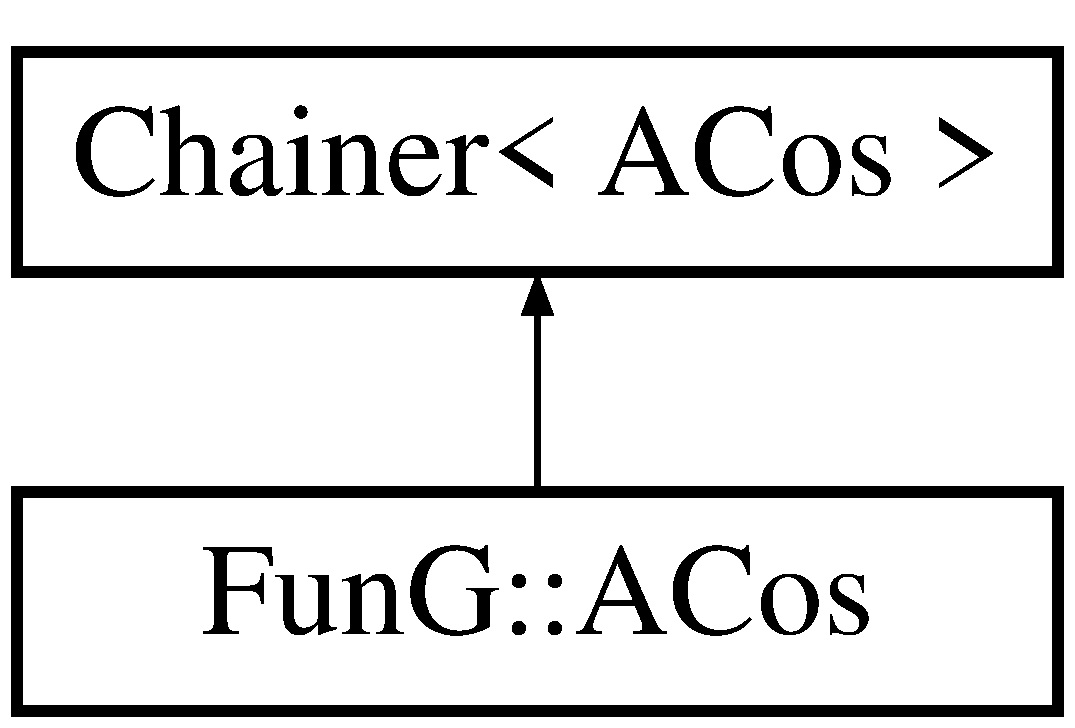
\includegraphics[height=2.000000cm]{structFunG_1_1ACos}
\end{center}
\end{figure}
\subsection*{Public Member Functions}
\begin{DoxyCompactItemize}
\item 
\hyperlink{structFunG_1_1ACos_a8096fe8fa93bb01b8fe3c1111aff300f}{A\-Cos} (double x=0.)
\begin{DoxyCompactList}\small\item\em Constructor. \end{DoxyCompactList}\item 
void \hyperlink{structFunG_1_1ACos_ad3870e46f4078161a3d586a44abc0c9c}{update} (double x)
\begin{DoxyCompactList}\small\item\em Set point of evaluation. \end{DoxyCompactList}\item 
double \hyperlink{structFunG_1_1ACos_abba20909d43d66485798fa56cf12d929}{d0} () const noexcept
\begin{DoxyCompactList}\small\item\em Function value. \end{DoxyCompactList}\item 
double \hyperlink{structFunG_1_1ACos_ad88d0c101e91f6183e16232614fb3471}{d1} (double dx=1) const 
\begin{DoxyCompactList}\small\item\em First (directional) derivative. \end{DoxyCompactList}\item 
double \hyperlink{structFunG_1_1ACos_a37917f9283d6b8414839283de92ab33f}{d2} (double dx=1, double dy=1) const 
\begin{DoxyCompactList}\small\item\em Second (directional) derivative. \end{DoxyCompactList}\item 
double \hyperlink{structFunG_1_1ACos_a5666e7232f2cf5c9257b34c6f165f477}{d3} (double dx=1, double dy=1, double dz=1) const 
\begin{DoxyCompactList}\small\item\em Third (directional) derivative. \end{DoxyCompactList}\end{DoxyCompactItemize}


\subsection{Detailed Description}
Arc cosine function including first three derivatives (based on acos(double) in $<$cmath$>$). 

For scalar functions directional derivatives are less interesting. Incorporating this function as building block for more complex functions requires directional derivatives. These occur during applications of the chain rule. 

\subsection{Constructor \& Destructor Documentation}
\hypertarget{structFunG_1_1ACos_a8096fe8fa93bb01b8fe3c1111aff300f}{\index{Fun\-G\-::\-A\-Cos@{Fun\-G\-::\-A\-Cos}!A\-Cos@{A\-Cos}}
\index{A\-Cos@{A\-Cos}!FunG::ACos@{Fun\-G\-::\-A\-Cos}}
\subsubsection[{A\-Cos}]{\setlength{\rightskip}{0pt plus 5cm}Fun\-G\-::\-A\-Cos\-::\-A\-Cos (
\begin{DoxyParamCaption}
\item[{double}]{x = {\ttfamily 0.}}
\end{DoxyParamCaption}
)\hspace{0.3cm}{\ttfamily [inline]}, {\ttfamily [explicit]}}}\label{structFunG_1_1ACos_a8096fe8fa93bb01b8fe3c1111aff300f}


Constructor. 


\begin{DoxyParams}{Parameters}
{\em x} & point of evaluation \\
\hline
\end{DoxyParams}


\subsection{Member Function Documentation}
\hypertarget{structFunG_1_1ACos_abba20909d43d66485798fa56cf12d929}{\index{Fun\-G\-::\-A\-Cos@{Fun\-G\-::\-A\-Cos}!d0@{d0}}
\index{d0@{d0}!FunG::ACos@{Fun\-G\-::\-A\-Cos}}
\subsubsection[{d0}]{\setlength{\rightskip}{0pt plus 5cm}double Fun\-G\-::\-A\-Cos\-::d0 (
\begin{DoxyParamCaption}
{}
\end{DoxyParamCaption}
) const\hspace{0.3cm}{\ttfamily [inline]}, {\ttfamily [noexcept]}}}\label{structFunG_1_1ACos_abba20909d43d66485798fa56cf12d929}


Function value. 

\hypertarget{structFunG_1_1ACos_ad88d0c101e91f6183e16232614fb3471}{\index{Fun\-G\-::\-A\-Cos@{Fun\-G\-::\-A\-Cos}!d1@{d1}}
\index{d1@{d1}!FunG::ACos@{Fun\-G\-::\-A\-Cos}}
\subsubsection[{d1}]{\setlength{\rightskip}{0pt plus 5cm}double Fun\-G\-::\-A\-Cos\-::d1 (
\begin{DoxyParamCaption}
\item[{double}]{dx = {\ttfamily 1}}
\end{DoxyParamCaption}
) const\hspace{0.3cm}{\ttfamily [inline]}}}\label{structFunG_1_1ACos_ad88d0c101e91f6183e16232614fb3471}


First (directional) derivative. 

\hypertarget{structFunG_1_1ACos_a37917f9283d6b8414839283de92ab33f}{\index{Fun\-G\-::\-A\-Cos@{Fun\-G\-::\-A\-Cos}!d2@{d2}}
\index{d2@{d2}!FunG::ACos@{Fun\-G\-::\-A\-Cos}}
\subsubsection[{d2}]{\setlength{\rightskip}{0pt plus 5cm}double Fun\-G\-::\-A\-Cos\-::d2 (
\begin{DoxyParamCaption}
\item[{double}]{dx = {\ttfamily 1}, }
\item[{double}]{dy = {\ttfamily 1}}
\end{DoxyParamCaption}
) const\hspace{0.3cm}{\ttfamily [inline]}}}\label{structFunG_1_1ACos_a37917f9283d6b8414839283de92ab33f}


Second (directional) derivative. 

\hypertarget{structFunG_1_1ACos_a5666e7232f2cf5c9257b34c6f165f477}{\index{Fun\-G\-::\-A\-Cos@{Fun\-G\-::\-A\-Cos}!d3@{d3}}
\index{d3@{d3}!FunG::ACos@{Fun\-G\-::\-A\-Cos}}
\subsubsection[{d3}]{\setlength{\rightskip}{0pt plus 5cm}double Fun\-G\-::\-A\-Cos\-::d3 (
\begin{DoxyParamCaption}
\item[{double}]{dx = {\ttfamily 1}, }
\item[{double}]{dy = {\ttfamily 1}, }
\item[{double}]{dz = {\ttfamily 1}}
\end{DoxyParamCaption}
) const\hspace{0.3cm}{\ttfamily [inline]}}}\label{structFunG_1_1ACos_a5666e7232f2cf5c9257b34c6f165f477}


Third (directional) derivative. 

\hypertarget{structFunG_1_1ACos_ad3870e46f4078161a3d586a44abc0c9c}{\index{Fun\-G\-::\-A\-Cos@{Fun\-G\-::\-A\-Cos}!update@{update}}
\index{update@{update}!FunG::ACos@{Fun\-G\-::\-A\-Cos}}
\subsubsection[{update}]{\setlength{\rightskip}{0pt plus 5cm}void Fun\-G\-::\-A\-Cos\-::update (
\begin{DoxyParamCaption}
\item[{double}]{x}
\end{DoxyParamCaption}
)\hspace{0.3cm}{\ttfamily [inline]}}}\label{structFunG_1_1ACos_ad3870e46f4078161a3d586a44abc0c9c}


Set point of evaluation. 



The documentation for this struct was generated from the following file\-:\begin{DoxyCompactItemize}
\item 
include/fung/cmath/\hyperlink{arccos_8hh}{arccos.\-hh}\end{DoxyCompactItemize}

\hypertarget{structFunG_1_1stringify_1_1ACos}{\section{Fun\-G\-:\-:stringify\-:\-:A\-Cos Struct Reference}
\label{structFunG_1_1stringify_1_1ACos}\index{Fun\-G\-::stringify\-::\-A\-Cos@{Fun\-G\-::stringify\-::\-A\-Cos}}
}


{\ttfamily \#include $<$arccos.\-hh$>$}

Inheritance diagram for Fun\-G\-:\-:stringify\-:\-:A\-Cos\-:\begin{figure}[H]
\begin{center}
\leavevmode
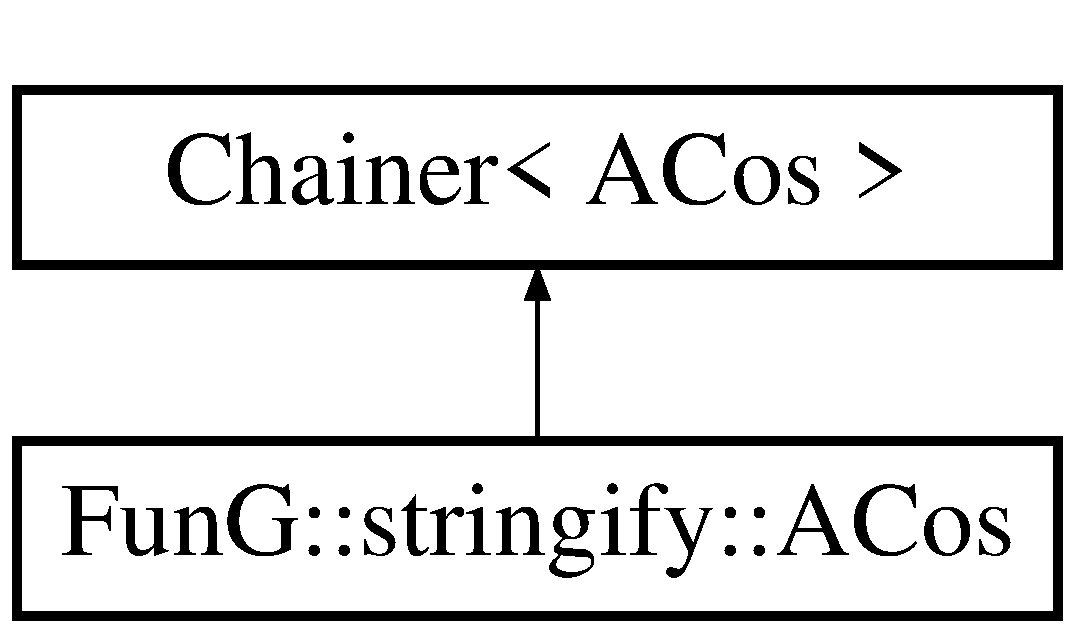
\includegraphics[height=2.000000cm]{structFunG_1_1stringify_1_1ACos}
\end{center}
\end{figure}
\subsection*{Public Member Functions}
\begin{DoxyCompactItemize}
\item 
\hyperlink{structFunG_1_1stringify_1_1ACos_ac88103a266ad60f4897f997054257efb}{A\-Cos} (std\-::string x=\char`\"{}x\char`\"{})
\begin{DoxyCompactList}\small\item\em Constructor. \end{DoxyCompactList}\item 
void \hyperlink{structFunG_1_1stringify_1_1ACos_acef19810a07f43d17721f04d2976bdd1}{update} (const std\-::string \&x)
\begin{DoxyCompactList}\small\item\em Set point of evaluation. \end{DoxyCompactList}\item 
std\-::string \hyperlink{structFunG_1_1stringify_1_1ACos_a01ca7b10f8cf8e3223bbdccc0cae1adc}{d0} () const noexcept
\begin{DoxyCompactList}\small\item\em Function value. \end{DoxyCompactList}\item 
std\-::string \hyperlink{structFunG_1_1stringify_1_1ACos_a892c5c2c69878c2c9ef23577d5c75ca3}{d1} (const std\-::string \&dx=\char`\"{}\char`\"{}) const 
\begin{DoxyCompactList}\small\item\em First (directional) derivative. \end{DoxyCompactList}\item 
std\-::string \hyperlink{structFunG_1_1stringify_1_1ACos_ab6c7fa17da02c623cff2b3e9f97d9bba}{d2} (const std\-::string \&dx=\char`\"{}\char`\"{}, const std\-::string \&dy=\char`\"{}\char`\"{}) const 
\begin{DoxyCompactList}\small\item\em Second (directional) derivative. \end{DoxyCompactList}\item 
std\-::string \hyperlink{structFunG_1_1stringify_1_1ACos_acb6586416672760c57a3c9344c873088}{d3} (const std\-::string \&dx=\char`\"{}\char`\"{}, const std\-::string \&dy=\char`\"{}\char`\"{}, const std\-::string \&dz=\char`\"{}\char`\"{}) const 
\begin{DoxyCompactList}\small\item\em Third (directional) derivative. \end{DoxyCompactList}\end{DoxyCompactItemize}


\subsection{Constructor \& Destructor Documentation}
\hypertarget{structFunG_1_1stringify_1_1ACos_ac88103a266ad60f4897f997054257efb}{\index{Fun\-G\-::stringify\-::\-A\-Cos@{Fun\-G\-::stringify\-::\-A\-Cos}!A\-Cos@{A\-Cos}}
\index{A\-Cos@{A\-Cos}!FunG::stringify::ACos@{Fun\-G\-::stringify\-::\-A\-Cos}}
\subsubsection[{A\-Cos}]{\setlength{\rightskip}{0pt plus 5cm}Fun\-G\-::stringify\-::\-A\-Cos\-::\-A\-Cos (
\begin{DoxyParamCaption}
\item[{std\-::string}]{x = {\ttfamily \char`\"{}x\char`\"{}}}
\end{DoxyParamCaption}
)\hspace{0.3cm}{\ttfamily [inline]}, {\ttfamily [explicit]}}}\label{structFunG_1_1stringify_1_1ACos_ac88103a266ad60f4897f997054257efb}


Constructor. 


\begin{DoxyParams}{Parameters}
{\em x} & point of evaluation \\
\hline
\end{DoxyParams}


\subsection{Member Function Documentation}
\hypertarget{structFunG_1_1stringify_1_1ACos_a01ca7b10f8cf8e3223bbdccc0cae1adc}{\index{Fun\-G\-::stringify\-::\-A\-Cos@{Fun\-G\-::stringify\-::\-A\-Cos}!d0@{d0}}
\index{d0@{d0}!FunG::stringify::ACos@{Fun\-G\-::stringify\-::\-A\-Cos}}
\subsubsection[{d0}]{\setlength{\rightskip}{0pt plus 5cm}std\-::string Fun\-G\-::stringify\-::\-A\-Cos\-::d0 (
\begin{DoxyParamCaption}
{}
\end{DoxyParamCaption}
) const\hspace{0.3cm}{\ttfamily [inline]}, {\ttfamily [noexcept]}}}\label{structFunG_1_1stringify_1_1ACos_a01ca7b10f8cf8e3223bbdccc0cae1adc}


Function value. 

\hypertarget{structFunG_1_1stringify_1_1ACos_a892c5c2c69878c2c9ef23577d5c75ca3}{\index{Fun\-G\-::stringify\-::\-A\-Cos@{Fun\-G\-::stringify\-::\-A\-Cos}!d1@{d1}}
\index{d1@{d1}!FunG::stringify::ACos@{Fun\-G\-::stringify\-::\-A\-Cos}}
\subsubsection[{d1}]{\setlength{\rightskip}{0pt plus 5cm}std\-::string Fun\-G\-::stringify\-::\-A\-Cos\-::d1 (
\begin{DoxyParamCaption}
\item[{const std\-::string \&}]{dx = {\ttfamily \char`\"{}\char`\"{}}}
\end{DoxyParamCaption}
) const\hspace{0.3cm}{\ttfamily [inline]}}}\label{structFunG_1_1stringify_1_1ACos_a892c5c2c69878c2c9ef23577d5c75ca3}


First (directional) derivative. 

\hypertarget{structFunG_1_1stringify_1_1ACos_ab6c7fa17da02c623cff2b3e9f97d9bba}{\index{Fun\-G\-::stringify\-::\-A\-Cos@{Fun\-G\-::stringify\-::\-A\-Cos}!d2@{d2}}
\index{d2@{d2}!FunG::stringify::ACos@{Fun\-G\-::stringify\-::\-A\-Cos}}
\subsubsection[{d2}]{\setlength{\rightskip}{0pt plus 5cm}std\-::string Fun\-G\-::stringify\-::\-A\-Cos\-::d2 (
\begin{DoxyParamCaption}
\item[{const std\-::string \&}]{dx = {\ttfamily \char`\"{}\char`\"{}}, }
\item[{const std\-::string \&}]{dy = {\ttfamily \char`\"{}\char`\"{}}}
\end{DoxyParamCaption}
) const\hspace{0.3cm}{\ttfamily [inline]}}}\label{structFunG_1_1stringify_1_1ACos_ab6c7fa17da02c623cff2b3e9f97d9bba}


Second (directional) derivative. 

\hypertarget{structFunG_1_1stringify_1_1ACos_acb6586416672760c57a3c9344c873088}{\index{Fun\-G\-::stringify\-::\-A\-Cos@{Fun\-G\-::stringify\-::\-A\-Cos}!d3@{d3}}
\index{d3@{d3}!FunG::stringify::ACos@{Fun\-G\-::stringify\-::\-A\-Cos}}
\subsubsection[{d3}]{\setlength{\rightskip}{0pt plus 5cm}std\-::string Fun\-G\-::stringify\-::\-A\-Cos\-::d3 (
\begin{DoxyParamCaption}
\item[{const std\-::string \&}]{dx = {\ttfamily \char`\"{}\char`\"{}}, }
\item[{const std\-::string \&}]{dy = {\ttfamily \char`\"{}\char`\"{}}, }
\item[{const std\-::string \&}]{dz = {\ttfamily \char`\"{}\char`\"{}}}
\end{DoxyParamCaption}
) const\hspace{0.3cm}{\ttfamily [inline]}}}\label{structFunG_1_1stringify_1_1ACos_acb6586416672760c57a3c9344c873088}


Third (directional) derivative. 

\hypertarget{structFunG_1_1stringify_1_1ACos_acef19810a07f43d17721f04d2976bdd1}{\index{Fun\-G\-::stringify\-::\-A\-Cos@{Fun\-G\-::stringify\-::\-A\-Cos}!update@{update}}
\index{update@{update}!FunG::stringify::ACos@{Fun\-G\-::stringify\-::\-A\-Cos}}
\subsubsection[{update}]{\setlength{\rightskip}{0pt plus 5cm}void Fun\-G\-::stringify\-::\-A\-Cos\-::update (
\begin{DoxyParamCaption}
\item[{const std\-::string \&}]{x}
\end{DoxyParamCaption}
)\hspace{0.3cm}{\ttfamily [inline]}}}\label{structFunG_1_1stringify_1_1ACos_acef19810a07f43d17721f04d2976bdd1}


Set point of evaluation. 



The documentation for this struct was generated from the following file\-:\begin{DoxyCompactItemize}
\item 
include/fung/stringify/cmath/\hyperlink{stringify_2cmath_2arccos_8hh}{arccos.\-hh}\end{DoxyCompactItemize}

\hypertarget{structFunG_1_1texify_1_1ACos}{\section{Fun\-G\-:\-:texify\-:\-:A\-Cos Struct Reference}
\label{structFunG_1_1texify_1_1ACos}\index{Fun\-G\-::texify\-::\-A\-Cos@{Fun\-G\-::texify\-::\-A\-Cos}}
}


{\ttfamily \#include $<$arccos.\-hh$>$}

Inheritance diagram for Fun\-G\-:\-:texify\-:\-:A\-Cos\-:\begin{figure}[H]
\begin{center}
\leavevmode
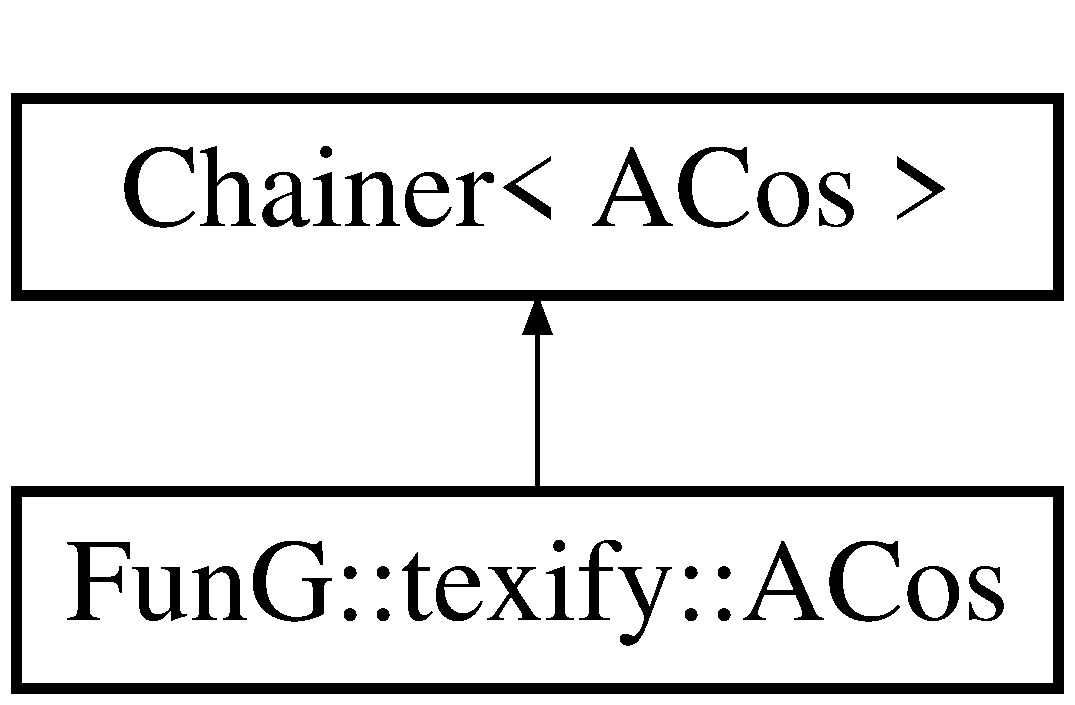
\includegraphics[height=2.000000cm]{structFunG_1_1texify_1_1ACos}
\end{center}
\end{figure}
\subsection*{Public Member Functions}
\begin{DoxyCompactItemize}
\item 
\hyperlink{structFunG_1_1texify_1_1ACos_a116d9f1d75b1c749d0d0daa69aad3c18}{A\-Cos} (std\-::string x=\char`\"{}x\char`\"{})
\begin{DoxyCompactList}\small\item\em Constructor. \end{DoxyCompactList}\item 
void \hyperlink{structFunG_1_1texify_1_1ACos_ae45f8aa8d0fd6a839089496225e776a9}{update} (const std\-::string \&x)
\begin{DoxyCompactList}\small\item\em Set point of evaluation. \end{DoxyCompactList}\item 
std\-::string \hyperlink{structFunG_1_1texify_1_1ACos_a3dbf7dbdb9c5a12cc603871d6b493881}{d0} () const noexcept
\begin{DoxyCompactList}\small\item\em Function value. \end{DoxyCompactList}\item 
std\-::string \hyperlink{structFunG_1_1texify_1_1ACos_ad4acc1259283ccd10dc72f5e8613667c}{d1} (const std\-::string \&dx=\char`\"{}\char`\"{}) const 
\begin{DoxyCompactList}\small\item\em First (directional) derivative. \end{DoxyCompactList}\item 
std\-::string \hyperlink{structFunG_1_1texify_1_1ACos_aed13b4dd95cf6f3eb75a1c3783412e22}{d2} (const std\-::string \&dx=\char`\"{}\char`\"{}, const std\-::string \&dy=\char`\"{}\char`\"{}) const 
\begin{DoxyCompactList}\small\item\em Second (directional) derivative. \end{DoxyCompactList}\item 
std\-::string \hyperlink{structFunG_1_1texify_1_1ACos_a8ba7333cf484c97d4160451a4ad88322}{d3} (const std\-::string \&dx=\char`\"{}\char`\"{}, const std\-::string \&dy=\char`\"{}\char`\"{}, const std\-::string \&dz=\char`\"{}\char`\"{}) const 
\begin{DoxyCompactList}\small\item\em Third (directional) derivative. \end{DoxyCompactList}\end{DoxyCompactItemize}


\subsection{Constructor \& Destructor Documentation}
\hypertarget{structFunG_1_1texify_1_1ACos_a116d9f1d75b1c749d0d0daa69aad3c18}{\index{Fun\-G\-::texify\-::\-A\-Cos@{Fun\-G\-::texify\-::\-A\-Cos}!A\-Cos@{A\-Cos}}
\index{A\-Cos@{A\-Cos}!FunG::texify::ACos@{Fun\-G\-::texify\-::\-A\-Cos}}
\subsubsection[{A\-Cos}]{\setlength{\rightskip}{0pt plus 5cm}Fun\-G\-::texify\-::\-A\-Cos\-::\-A\-Cos (
\begin{DoxyParamCaption}
\item[{std\-::string}]{x = {\ttfamily \char`\"{}x\char`\"{}}}
\end{DoxyParamCaption}
)\hspace{0.3cm}{\ttfamily [inline]}, {\ttfamily [explicit]}}}\label{structFunG_1_1texify_1_1ACos_a116d9f1d75b1c749d0d0daa69aad3c18}


Constructor. 


\begin{DoxyParams}{Parameters}
{\em x} & point of evaluation \\
\hline
\end{DoxyParams}


\subsection{Member Function Documentation}
\hypertarget{structFunG_1_1texify_1_1ACos_a3dbf7dbdb9c5a12cc603871d6b493881}{\index{Fun\-G\-::texify\-::\-A\-Cos@{Fun\-G\-::texify\-::\-A\-Cos}!d0@{d0}}
\index{d0@{d0}!FunG::texify::ACos@{Fun\-G\-::texify\-::\-A\-Cos}}
\subsubsection[{d0}]{\setlength{\rightskip}{0pt plus 5cm}std\-::string Fun\-G\-::texify\-::\-A\-Cos\-::d0 (
\begin{DoxyParamCaption}
{}
\end{DoxyParamCaption}
) const\hspace{0.3cm}{\ttfamily [inline]}, {\ttfamily [noexcept]}}}\label{structFunG_1_1texify_1_1ACos_a3dbf7dbdb9c5a12cc603871d6b493881}


Function value. 

\hypertarget{structFunG_1_1texify_1_1ACos_ad4acc1259283ccd10dc72f5e8613667c}{\index{Fun\-G\-::texify\-::\-A\-Cos@{Fun\-G\-::texify\-::\-A\-Cos}!d1@{d1}}
\index{d1@{d1}!FunG::texify::ACos@{Fun\-G\-::texify\-::\-A\-Cos}}
\subsubsection[{d1}]{\setlength{\rightskip}{0pt plus 5cm}std\-::string Fun\-G\-::texify\-::\-A\-Cos\-::d1 (
\begin{DoxyParamCaption}
\item[{const std\-::string \&}]{dx = {\ttfamily \char`\"{}\char`\"{}}}
\end{DoxyParamCaption}
) const\hspace{0.3cm}{\ttfamily [inline]}}}\label{structFunG_1_1texify_1_1ACos_ad4acc1259283ccd10dc72f5e8613667c}


First (directional) derivative. 

\hypertarget{structFunG_1_1texify_1_1ACos_aed13b4dd95cf6f3eb75a1c3783412e22}{\index{Fun\-G\-::texify\-::\-A\-Cos@{Fun\-G\-::texify\-::\-A\-Cos}!d2@{d2}}
\index{d2@{d2}!FunG::texify::ACos@{Fun\-G\-::texify\-::\-A\-Cos}}
\subsubsection[{d2}]{\setlength{\rightskip}{0pt plus 5cm}std\-::string Fun\-G\-::texify\-::\-A\-Cos\-::d2 (
\begin{DoxyParamCaption}
\item[{const std\-::string \&}]{dx = {\ttfamily \char`\"{}\char`\"{}}, }
\item[{const std\-::string \&}]{dy = {\ttfamily \char`\"{}\char`\"{}}}
\end{DoxyParamCaption}
) const\hspace{0.3cm}{\ttfamily [inline]}}}\label{structFunG_1_1texify_1_1ACos_aed13b4dd95cf6f3eb75a1c3783412e22}


Second (directional) derivative. 

\hypertarget{structFunG_1_1texify_1_1ACos_a8ba7333cf484c97d4160451a4ad88322}{\index{Fun\-G\-::texify\-::\-A\-Cos@{Fun\-G\-::texify\-::\-A\-Cos}!d3@{d3}}
\index{d3@{d3}!FunG::texify::ACos@{Fun\-G\-::texify\-::\-A\-Cos}}
\subsubsection[{d3}]{\setlength{\rightskip}{0pt plus 5cm}std\-::string Fun\-G\-::texify\-::\-A\-Cos\-::d3 (
\begin{DoxyParamCaption}
\item[{const std\-::string \&}]{dx = {\ttfamily \char`\"{}\char`\"{}}, }
\item[{const std\-::string \&}]{dy = {\ttfamily \char`\"{}\char`\"{}}, }
\item[{const std\-::string \&}]{dz = {\ttfamily \char`\"{}\char`\"{}}}
\end{DoxyParamCaption}
) const\hspace{0.3cm}{\ttfamily [inline]}}}\label{structFunG_1_1texify_1_1ACos_a8ba7333cf484c97d4160451a4ad88322}


Third (directional) derivative. 

\hypertarget{structFunG_1_1texify_1_1ACos_ae45f8aa8d0fd6a839089496225e776a9}{\index{Fun\-G\-::texify\-::\-A\-Cos@{Fun\-G\-::texify\-::\-A\-Cos}!update@{update}}
\index{update@{update}!FunG::texify::ACos@{Fun\-G\-::texify\-::\-A\-Cos}}
\subsubsection[{update}]{\setlength{\rightskip}{0pt plus 5cm}void Fun\-G\-::texify\-::\-A\-Cos\-::update (
\begin{DoxyParamCaption}
\item[{const std\-::string \&}]{x}
\end{DoxyParamCaption}
)\hspace{0.3cm}{\ttfamily [inline]}}}\label{structFunG_1_1texify_1_1ACos_ae45f8aa8d0fd6a839089496225e776a9}


Set point of evaluation. 



The documentation for this struct was generated from the following file\-:\begin{DoxyCompactItemize}
\item 
include/fung/cmath/texify/\hyperlink{texify_2arccos_8hh}{arccos.\-hh}\end{DoxyCompactItemize}

\hypertarget{structFunG_1_1Concepts_1_1ArithmeticConcept}{\section{\-Fun\-G\-:\-:\-Concepts\-:\-:\-Arithmetic\-Concept \-Struct \-Reference}
\label{structFunG_1_1Concepts_1_1ArithmeticConcept}\index{\-Fun\-G\-::\-Concepts\-::\-Arithmetic\-Concept@{\-Fun\-G\-::\-Concepts\-::\-Arithmetic\-Concept}}
}


\-Requirements on input types.  




{\ttfamily \#include $<$concepts.\-hh$>$}

\-Inheritance diagram for \-Fun\-G\-:\-:\-Concepts\-:\-:\-Arithmetic\-Concept\-:\begin{figure}[H]
\begin{center}
\leavevmode
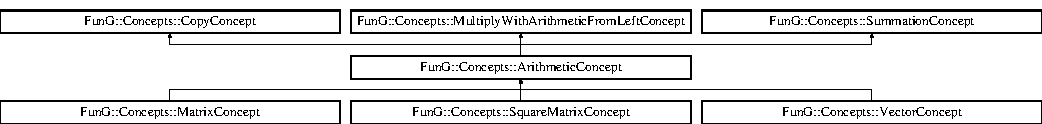
\includegraphics[height=1.661721cm]{structFunG_1_1Concepts_1_1ArithmeticConcept}
\end{center}
\end{figure}


\subsection{\-Detailed \-Description}
\-Requirements on input types. 

\-Multiplication between different matrices is not checked here, since this would require to provide all possible matrices to multiply a matrix of type \-Arg with. 

\-The documentation for this struct was generated from the following file\-:\begin{DoxyCompactItemize}
\item 
fung/\hyperlink{concepts_8hh}{concepts.\-hh}\end{DoxyCompactItemize}

\hypertarget{structFunG_1_1Concepts_1_1ArithmeticConceptCheck}{\section{Fun\-G\-:\-:Concepts\-:\-:Arithmetic\-Concept\-Check$<$ Arg $>$ Struct Template Reference}
\label{structFunG_1_1Concepts_1_1ArithmeticConceptCheck}\index{Fun\-G\-::\-Concepts\-::\-Arithmetic\-Concept\-Check$<$ Arg $>$@{Fun\-G\-::\-Concepts\-::\-Arithmetic\-Concept\-Check$<$ Arg $>$}}
}


Static check if the requirements of \hyperlink{structFunG_1_1Concepts_1_1ArithmeticConcept}{Arithmetic\-Concept} are satisfied.  




{\ttfamily \#include $<$concept\-\_\-check.\-hh$>$}

Inheritance diagram for Fun\-G\-:\-:Concepts\-:\-:Arithmetic\-Concept\-Check$<$ Arg $>$\-:\begin{figure}[H]
\begin{center}
\leavevmode
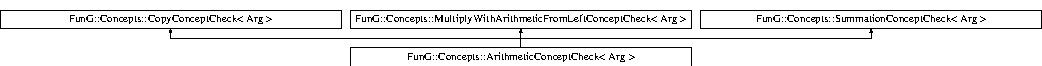
\includegraphics[height=0.893142cm]{structFunG_1_1Concepts_1_1ArithmeticConceptCheck}
\end{center}
\end{figure}


\subsection{Detailed Description}
\subsubsection*{template$<$class Arg$>$struct Fun\-G\-::\-Concepts\-::\-Arithmetic\-Concept\-Check$<$ Arg $>$}

Static check if the requirements of \hyperlink{structFunG_1_1Concepts_1_1ArithmeticConcept}{Arithmetic\-Concept} are satisfied. 

The documentation for this struct was generated from the following file\-:\begin{DoxyCompactItemize}
\item 
fung/\hyperlink{concept__check_8hh}{concept\-\_\-check.\-hh}\end{DoxyCompactItemize}

\hypertarget{structFunG_1_1ASin}{}\section{FunG\+:\+:A\+Sin Struct Reference}
\label{structFunG_1_1ASin}\index{Fun\+G\+::\+A\+Sin@{Fun\+G\+::\+A\+Sin}}


Arc sine function including first three derivatives (based on asin(double) in $<$cmath$>$).  




{\ttfamily \#include $<$arcsine.\+hh$>$}

Inheritance diagram for FunG\+:\+:A\+Sin\+:\begin{figure}[H]
\begin{center}
\leavevmode
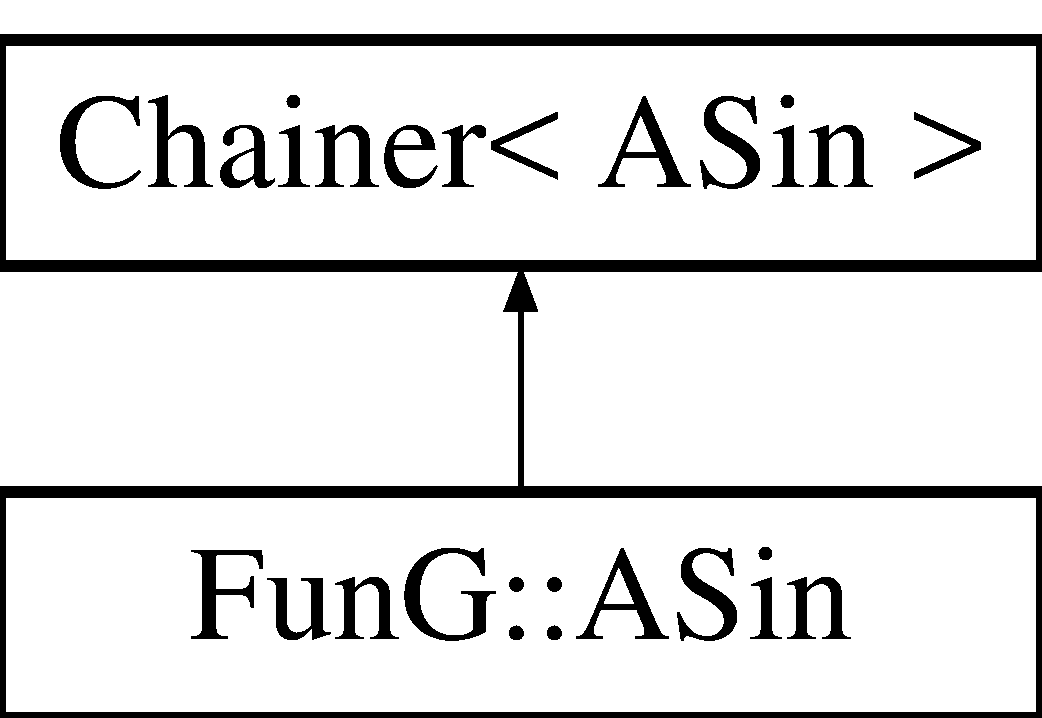
\includegraphics[height=2.000000cm]{structFunG_1_1ASin}
\end{center}
\end{figure}
\subsection*{Public Member Functions}
\begin{DoxyCompactItemize}
\item 
\hyperlink{structFunG_1_1ASin_aea477c9658dc3cea15cd77aa637b5ce4}{A\+Sin} (double x=0.)
\begin{DoxyCompactList}\small\item\em Constructor. \end{DoxyCompactList}\item 
void \hyperlink{structFunG_1_1ASin_a0c7e3aa8b532914de2068b3bc74d57f1}{update} (double x)
\begin{DoxyCompactList}\small\item\em Set point of evaluation. \end{DoxyCompactList}\item 
double \hyperlink{structFunG_1_1ASin_a9c3b2d30afbd9d258b7bf30b425f5600}{d0} () const noexcept
\begin{DoxyCompactList}\small\item\em Function value. \end{DoxyCompactList}\item 
double \hyperlink{structFunG_1_1ASin_a0468608cbecdcc4d8d5eca641232ceba}{d1} (double dx=1) const 
\begin{DoxyCompactList}\small\item\em First (directional) derivative. \end{DoxyCompactList}\item 
double \hyperlink{structFunG_1_1ASin_a3bf0627e743505d38f04e9d9132331df}{d2} (double dx=1, double dy=1) const 
\begin{DoxyCompactList}\small\item\em Second (directional) derivative. \end{DoxyCompactList}\item 
double \hyperlink{structFunG_1_1ASin_a50f2fbd6e12b64492ef63c732f0f82f1}{d3} (double dx=1, double dy=1, double dz=1) const 
\begin{DoxyCompactList}\small\item\em Third (directional) derivative. \end{DoxyCompactList}\end{DoxyCompactItemize}


\subsection{Detailed Description}
Arc sine function including first three derivatives (based on asin(double) in $<$cmath$>$). 

For scalar functions directional derivatives are less interesting. Incorporating this function as building block for more complex functions requires directional derivatives. These occur during applications of the chain rule. 

\subsection{Constructor \& Destructor Documentation}
\index{Fun\+G\+::\+A\+Sin@{Fun\+G\+::\+A\+Sin}!A\+Sin@{A\+Sin}}
\index{A\+Sin@{A\+Sin}!Fun\+G\+::\+A\+Sin@{Fun\+G\+::\+A\+Sin}}
\subsubsection[{\texorpdfstring{A\+Sin(double x=0.)}{ASin(double x=0.)}}]{\setlength{\rightskip}{0pt plus 5cm}Fun\+G\+::\+A\+Sin\+::\+A\+Sin (
\begin{DoxyParamCaption}
\item[{double}]{x = {\ttfamily 0.}}
\end{DoxyParamCaption}
)\hspace{0.3cm}{\ttfamily [inline]}, {\ttfamily [explicit]}}\hypertarget{structFunG_1_1ASin_aea477c9658dc3cea15cd77aa637b5ce4}{}\label{structFunG_1_1ASin_aea477c9658dc3cea15cd77aa637b5ce4}


Constructor. 


\begin{DoxyParams}{Parameters}
{\em x} & point of evaluation \\
\hline
\end{DoxyParams}


\subsection{Member Function Documentation}
\index{Fun\+G\+::\+A\+Sin@{Fun\+G\+::\+A\+Sin}!d0@{d0}}
\index{d0@{d0}!Fun\+G\+::\+A\+Sin@{Fun\+G\+::\+A\+Sin}}
\subsubsection[{\texorpdfstring{d0() const noexcept}{d0() const noexcept}}]{\setlength{\rightskip}{0pt plus 5cm}double Fun\+G\+::\+A\+Sin\+::d0 (
\begin{DoxyParamCaption}
{}
\end{DoxyParamCaption}
) const\hspace{0.3cm}{\ttfamily [inline]}, {\ttfamily [noexcept]}}\hypertarget{structFunG_1_1ASin_a9c3b2d30afbd9d258b7bf30b425f5600}{}\label{structFunG_1_1ASin_a9c3b2d30afbd9d258b7bf30b425f5600}


Function value. 

\index{Fun\+G\+::\+A\+Sin@{Fun\+G\+::\+A\+Sin}!d1@{d1}}
\index{d1@{d1}!Fun\+G\+::\+A\+Sin@{Fun\+G\+::\+A\+Sin}}
\subsubsection[{\texorpdfstring{d1(double dx=1) const }{d1(double dx=1) const }}]{\setlength{\rightskip}{0pt plus 5cm}double Fun\+G\+::\+A\+Sin\+::d1 (
\begin{DoxyParamCaption}
\item[{double}]{dx = {\ttfamily 1}}
\end{DoxyParamCaption}
) const\hspace{0.3cm}{\ttfamily [inline]}}\hypertarget{structFunG_1_1ASin_a0468608cbecdcc4d8d5eca641232ceba}{}\label{structFunG_1_1ASin_a0468608cbecdcc4d8d5eca641232ceba}


First (directional) derivative. 

\index{Fun\+G\+::\+A\+Sin@{Fun\+G\+::\+A\+Sin}!d2@{d2}}
\index{d2@{d2}!Fun\+G\+::\+A\+Sin@{Fun\+G\+::\+A\+Sin}}
\subsubsection[{\texorpdfstring{d2(double dx=1, double dy=1) const }{d2(double dx=1, double dy=1) const }}]{\setlength{\rightskip}{0pt plus 5cm}double Fun\+G\+::\+A\+Sin\+::d2 (
\begin{DoxyParamCaption}
\item[{double}]{dx = {\ttfamily 1}, }
\item[{double}]{dy = {\ttfamily 1}}
\end{DoxyParamCaption}
) const\hspace{0.3cm}{\ttfamily [inline]}}\hypertarget{structFunG_1_1ASin_a3bf0627e743505d38f04e9d9132331df}{}\label{structFunG_1_1ASin_a3bf0627e743505d38f04e9d9132331df}


Second (directional) derivative. 

\index{Fun\+G\+::\+A\+Sin@{Fun\+G\+::\+A\+Sin}!d3@{d3}}
\index{d3@{d3}!Fun\+G\+::\+A\+Sin@{Fun\+G\+::\+A\+Sin}}
\subsubsection[{\texorpdfstring{d3(double dx=1, double dy=1, double dz=1) const }{d3(double dx=1, double dy=1, double dz=1) const }}]{\setlength{\rightskip}{0pt plus 5cm}double Fun\+G\+::\+A\+Sin\+::d3 (
\begin{DoxyParamCaption}
\item[{double}]{dx = {\ttfamily 1}, }
\item[{double}]{dy = {\ttfamily 1}, }
\item[{double}]{dz = {\ttfamily 1}}
\end{DoxyParamCaption}
) const\hspace{0.3cm}{\ttfamily [inline]}}\hypertarget{structFunG_1_1ASin_a50f2fbd6e12b64492ef63c732f0f82f1}{}\label{structFunG_1_1ASin_a50f2fbd6e12b64492ef63c732f0f82f1}


Third (directional) derivative. 

\index{Fun\+G\+::\+A\+Sin@{Fun\+G\+::\+A\+Sin}!update@{update}}
\index{update@{update}!Fun\+G\+::\+A\+Sin@{Fun\+G\+::\+A\+Sin}}
\subsubsection[{\texorpdfstring{update(double x)}{update(double x)}}]{\setlength{\rightskip}{0pt plus 5cm}void Fun\+G\+::\+A\+Sin\+::update (
\begin{DoxyParamCaption}
\item[{double}]{x}
\end{DoxyParamCaption}
)\hspace{0.3cm}{\ttfamily [inline]}}\hypertarget{structFunG_1_1ASin_a0c7e3aa8b532914de2068b3bc74d57f1}{}\label{structFunG_1_1ASin_a0c7e3aa8b532914de2068b3bc74d57f1}


Set point of evaluation. 



The documentation for this struct was generated from the following file\+:\begin{DoxyCompactItemize}
\item 
include/fung/cmath/\hyperlink{arcsine_8hh}{arcsine.\+hh}\end{DoxyCompactItemize}

\hypertarget{structFunG_1_1texify_1_1ASin}{\section{Fun\-G\-:\-:texify\-:\-:A\-Sin Struct Reference}
\label{structFunG_1_1texify_1_1ASin}\index{Fun\-G\-::texify\-::\-A\-Sin@{Fun\-G\-::texify\-::\-A\-Sin}}
}


{\ttfamily \#include $<$arcsine.\-hh$>$}

Inheritance diagram for Fun\-G\-:\-:texify\-:\-:A\-Sin\-:\begin{figure}[H]
\begin{center}
\leavevmode
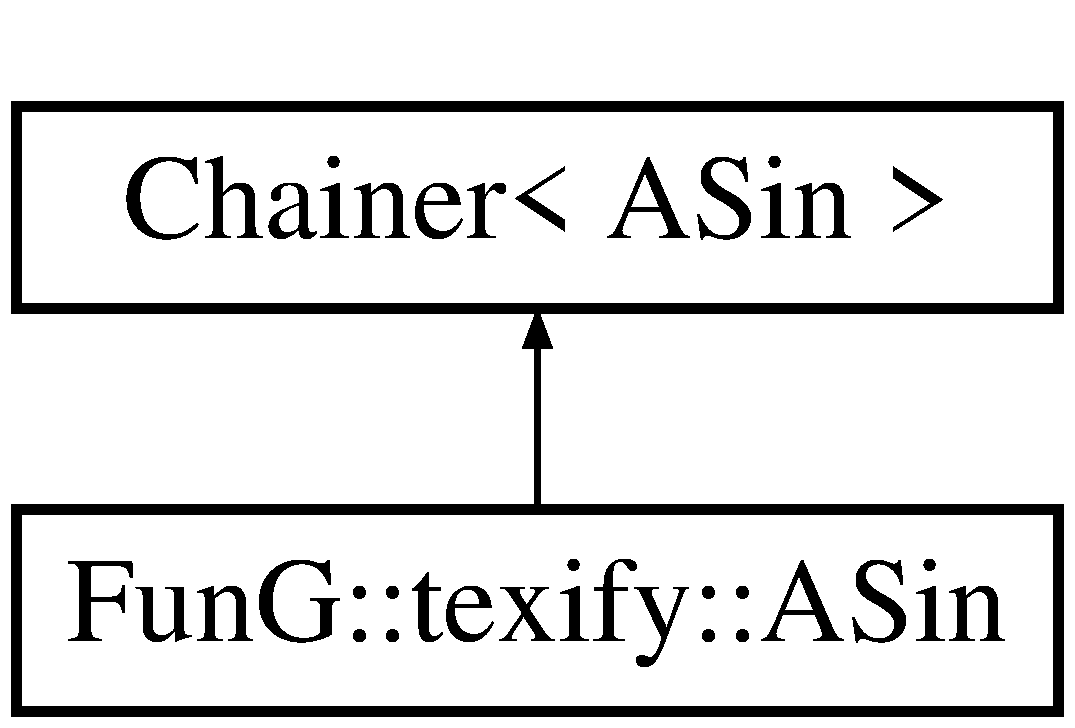
\includegraphics[height=2.000000cm]{structFunG_1_1texify_1_1ASin}
\end{center}
\end{figure}
\subsection*{Public Member Functions}
\begin{DoxyCompactItemize}
\item 
\hyperlink{structFunG_1_1texify_1_1ASin_a8221eb34628298fb26ca8de5f885f974}{A\-Sin} (const std\-::string \&x=\char`\"{}x\char`\"{})
\begin{DoxyCompactList}\small\item\em Constructor. \end{DoxyCompactList}\item 
void \hyperlink{structFunG_1_1texify_1_1ASin_a7ab289642f3643132c4566c9166f8e08}{update} (const std\-::string \&x)
\begin{DoxyCompactList}\small\item\em Set point of evaluation. \end{DoxyCompactList}\item 
std\-::string \hyperlink{structFunG_1_1texify_1_1ASin_a5f87a42235c262e2e739d218d2830de7}{d0} () const noexcept
\begin{DoxyCompactList}\small\item\em Function value. \end{DoxyCompactList}\item 
std\-::string \hyperlink{structFunG_1_1texify_1_1ASin_a29ea3b1a1a439c28d7b8f62b06c8ba37}{d1} (const std\-::string \&dx=\char`\"{}\char`\"{}) const 
\begin{DoxyCompactList}\small\item\em First (directional) derivative. \end{DoxyCompactList}\item 
std\-::string \hyperlink{structFunG_1_1texify_1_1ASin_af4a439065864319c0f6d757fbd91163f}{d2} (const std\-::string \&dx=\char`\"{}\char`\"{}, const std\-::string \&dy=\char`\"{}\char`\"{}) const 
\begin{DoxyCompactList}\small\item\em Second (directional) derivative. \end{DoxyCompactList}\item 
std\-::string \hyperlink{structFunG_1_1texify_1_1ASin_a713815d60bc379b274a6cdceaa5fa9f9}{d3} (const std\-::string \&dx=\char`\"{}\char`\"{}, const std\-::string \&dy=\char`\"{}\char`\"{}, const std\-::string \&dz=\char`\"{}\char`\"{}) const 
\begin{DoxyCompactList}\small\item\em Third (directional) derivative. \end{DoxyCompactList}\end{DoxyCompactItemize}


\subsection{Constructor \& Destructor Documentation}
\hypertarget{structFunG_1_1texify_1_1ASin_a8221eb34628298fb26ca8de5f885f974}{\index{Fun\-G\-::texify\-::\-A\-Sin@{Fun\-G\-::texify\-::\-A\-Sin}!A\-Sin@{A\-Sin}}
\index{A\-Sin@{A\-Sin}!FunG::texify::ASin@{Fun\-G\-::texify\-::\-A\-Sin}}
\subsubsection[{A\-Sin}]{\setlength{\rightskip}{0pt plus 5cm}Fun\-G\-::texify\-::\-A\-Sin\-::\-A\-Sin (
\begin{DoxyParamCaption}
\item[{const std\-::string \&}]{x = {\ttfamily \char`\"{}x\char`\"{}}}
\end{DoxyParamCaption}
)\hspace{0.3cm}{\ttfamily [inline]}, {\ttfamily [explicit]}}}\label{structFunG_1_1texify_1_1ASin_a8221eb34628298fb26ca8de5f885f974}


Constructor. 


\begin{DoxyParams}{Parameters}
{\em x} & point of evaluation \\
\hline
\end{DoxyParams}


\subsection{Member Function Documentation}
\hypertarget{structFunG_1_1texify_1_1ASin_a5f87a42235c262e2e739d218d2830de7}{\index{Fun\-G\-::texify\-::\-A\-Sin@{Fun\-G\-::texify\-::\-A\-Sin}!d0@{d0}}
\index{d0@{d0}!FunG::texify::ASin@{Fun\-G\-::texify\-::\-A\-Sin}}
\subsubsection[{d0}]{\setlength{\rightskip}{0pt plus 5cm}std\-::string Fun\-G\-::texify\-::\-A\-Sin\-::d0 (
\begin{DoxyParamCaption}
{}
\end{DoxyParamCaption}
) const\hspace{0.3cm}{\ttfamily [inline]}, {\ttfamily [noexcept]}}}\label{structFunG_1_1texify_1_1ASin_a5f87a42235c262e2e739d218d2830de7}


Function value. 

\hypertarget{structFunG_1_1texify_1_1ASin_a29ea3b1a1a439c28d7b8f62b06c8ba37}{\index{Fun\-G\-::texify\-::\-A\-Sin@{Fun\-G\-::texify\-::\-A\-Sin}!d1@{d1}}
\index{d1@{d1}!FunG::texify::ASin@{Fun\-G\-::texify\-::\-A\-Sin}}
\subsubsection[{d1}]{\setlength{\rightskip}{0pt plus 5cm}std\-::string Fun\-G\-::texify\-::\-A\-Sin\-::d1 (
\begin{DoxyParamCaption}
\item[{const std\-::string \&}]{dx = {\ttfamily \char`\"{}\char`\"{}}}
\end{DoxyParamCaption}
) const\hspace{0.3cm}{\ttfamily [inline]}}}\label{structFunG_1_1texify_1_1ASin_a29ea3b1a1a439c28d7b8f62b06c8ba37}


First (directional) derivative. 

\hypertarget{structFunG_1_1texify_1_1ASin_af4a439065864319c0f6d757fbd91163f}{\index{Fun\-G\-::texify\-::\-A\-Sin@{Fun\-G\-::texify\-::\-A\-Sin}!d2@{d2}}
\index{d2@{d2}!FunG::texify::ASin@{Fun\-G\-::texify\-::\-A\-Sin}}
\subsubsection[{d2}]{\setlength{\rightskip}{0pt plus 5cm}std\-::string Fun\-G\-::texify\-::\-A\-Sin\-::d2 (
\begin{DoxyParamCaption}
\item[{const std\-::string \&}]{dx = {\ttfamily \char`\"{}\char`\"{}}, }
\item[{const std\-::string \&}]{dy = {\ttfamily \char`\"{}\char`\"{}}}
\end{DoxyParamCaption}
) const\hspace{0.3cm}{\ttfamily [inline]}}}\label{structFunG_1_1texify_1_1ASin_af4a439065864319c0f6d757fbd91163f}


Second (directional) derivative. 

\hypertarget{structFunG_1_1texify_1_1ASin_a713815d60bc379b274a6cdceaa5fa9f9}{\index{Fun\-G\-::texify\-::\-A\-Sin@{Fun\-G\-::texify\-::\-A\-Sin}!d3@{d3}}
\index{d3@{d3}!FunG::texify::ASin@{Fun\-G\-::texify\-::\-A\-Sin}}
\subsubsection[{d3}]{\setlength{\rightskip}{0pt plus 5cm}std\-::string Fun\-G\-::texify\-::\-A\-Sin\-::d3 (
\begin{DoxyParamCaption}
\item[{const std\-::string \&}]{dx = {\ttfamily \char`\"{}\char`\"{}}, }
\item[{const std\-::string \&}]{dy = {\ttfamily \char`\"{}\char`\"{}}, }
\item[{const std\-::string \&}]{dz = {\ttfamily \char`\"{}\char`\"{}}}
\end{DoxyParamCaption}
) const\hspace{0.3cm}{\ttfamily [inline]}}}\label{structFunG_1_1texify_1_1ASin_a713815d60bc379b274a6cdceaa5fa9f9}


Third (directional) derivative. 

\hypertarget{structFunG_1_1texify_1_1ASin_a7ab289642f3643132c4566c9166f8e08}{\index{Fun\-G\-::texify\-::\-A\-Sin@{Fun\-G\-::texify\-::\-A\-Sin}!update@{update}}
\index{update@{update}!FunG::texify::ASin@{Fun\-G\-::texify\-::\-A\-Sin}}
\subsubsection[{update}]{\setlength{\rightskip}{0pt plus 5cm}void Fun\-G\-::texify\-::\-A\-Sin\-::update (
\begin{DoxyParamCaption}
\item[{const std\-::string \&}]{x}
\end{DoxyParamCaption}
)\hspace{0.3cm}{\ttfamily [inline]}}}\label{structFunG_1_1texify_1_1ASin_a7ab289642f3643132c4566c9166f8e08}


Set point of evaluation. 



The documentation for this struct was generated from the following file\-:\begin{DoxyCompactItemize}
\item 
include/fung/cmath/texify/\hyperlink{texify_2arcsine_8hh}{arcsine.\-hh}\end{DoxyCompactItemize}

\hypertarget{structFunG_1_1stringify_1_1ASin}{\section{Fun\-G\-:\-:stringify\-:\-:A\-Sin Struct Reference}
\label{structFunG_1_1stringify_1_1ASin}\index{Fun\-G\-::stringify\-::\-A\-Sin@{Fun\-G\-::stringify\-::\-A\-Sin}}
}


{\ttfamily \#include $<$arcsine.\-hh$>$}

Inheritance diagram for Fun\-G\-:\-:stringify\-:\-:A\-Sin\-:\begin{figure}[H]
\begin{center}
\leavevmode
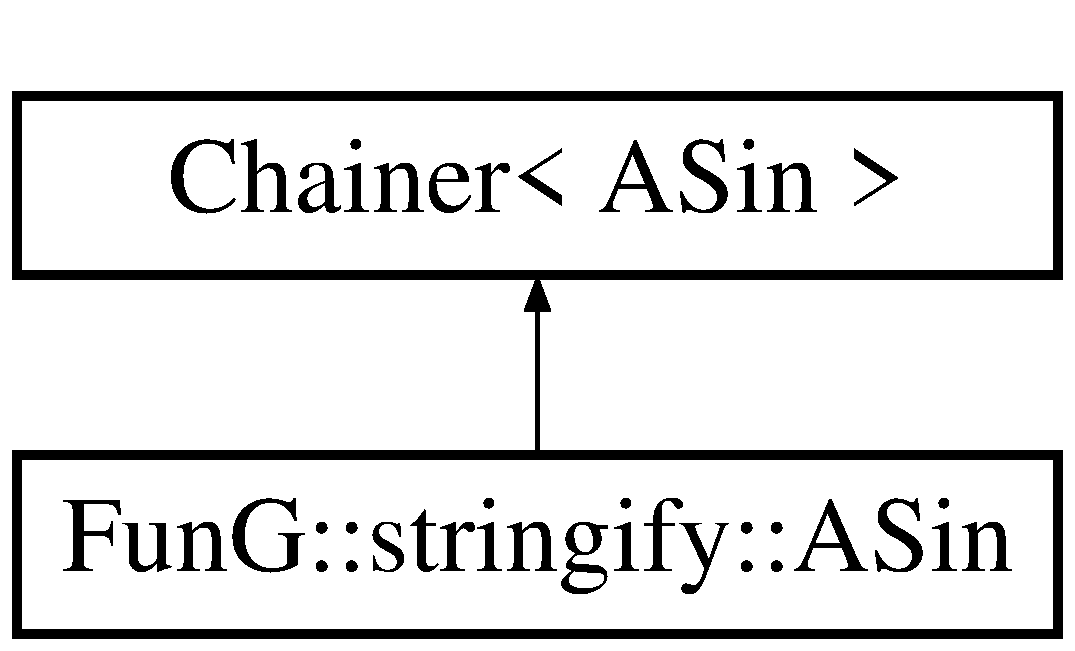
\includegraphics[height=2.000000cm]{structFunG_1_1stringify_1_1ASin}
\end{center}
\end{figure}
\subsection*{Public Member Functions}
\begin{DoxyCompactItemize}
\item 
\hyperlink{structFunG_1_1stringify_1_1ASin_a45f7b447d7830fc5ca2471b8ecad3aea}{A\-Sin} (const std\-::string \&x=\char`\"{}x\char`\"{})
\begin{DoxyCompactList}\small\item\em Constructor. \end{DoxyCompactList}\item 
void \hyperlink{structFunG_1_1stringify_1_1ASin_ad3d41fb5fc4f4627dd46b50203e50293}{update} (const std\-::string \&x)
\begin{DoxyCompactList}\small\item\em Set point of evaluation. \end{DoxyCompactList}\item 
std\-::string \hyperlink{structFunG_1_1stringify_1_1ASin_af0ede3a3b0de798bca4890d43232b760}{d0} () const noexcept
\begin{DoxyCompactList}\small\item\em Function value. \end{DoxyCompactList}\item 
std\-::string \hyperlink{structFunG_1_1stringify_1_1ASin_a19425e85304dc6c4b4bcbb50e82f5bfe}{d1} (const std\-::string \&dx=\char`\"{}\char`\"{}) const 
\begin{DoxyCompactList}\small\item\em First (directional) derivative. \end{DoxyCompactList}\item 
std\-::string \hyperlink{structFunG_1_1stringify_1_1ASin_a6d2de4322435dbe7feaaad63c2468f72}{d2} (const std\-::string \&dx=\char`\"{}\char`\"{}, const std\-::string \&dy=\char`\"{}\char`\"{}) const 
\begin{DoxyCompactList}\small\item\em Second (directional) derivative. \end{DoxyCompactList}\item 
std\-::string \hyperlink{structFunG_1_1stringify_1_1ASin_ae73b155636f481bab7b2dea7153fc923}{d3} (const std\-::string \&dx=\char`\"{}\char`\"{}, const std\-::string \&dy=\char`\"{}\char`\"{}, const std\-::string \&dz=\char`\"{}\char`\"{}) const 
\begin{DoxyCompactList}\small\item\em Third (directional) derivative. \end{DoxyCompactList}\end{DoxyCompactItemize}


\subsection{Constructor \& Destructor Documentation}
\hypertarget{structFunG_1_1stringify_1_1ASin_a45f7b447d7830fc5ca2471b8ecad3aea}{\index{Fun\-G\-::stringify\-::\-A\-Sin@{Fun\-G\-::stringify\-::\-A\-Sin}!A\-Sin@{A\-Sin}}
\index{A\-Sin@{A\-Sin}!FunG::stringify::ASin@{Fun\-G\-::stringify\-::\-A\-Sin}}
\subsubsection[{A\-Sin}]{\setlength{\rightskip}{0pt plus 5cm}Fun\-G\-::stringify\-::\-A\-Sin\-::\-A\-Sin (
\begin{DoxyParamCaption}
\item[{const std\-::string \&}]{x = {\ttfamily \char`\"{}x\char`\"{}}}
\end{DoxyParamCaption}
)\hspace{0.3cm}{\ttfamily [inline]}, {\ttfamily [explicit]}}}\label{structFunG_1_1stringify_1_1ASin_a45f7b447d7830fc5ca2471b8ecad3aea}


Constructor. 


\begin{DoxyParams}{Parameters}
{\em x} & point of evaluation \\
\hline
\end{DoxyParams}


\subsection{Member Function Documentation}
\hypertarget{structFunG_1_1stringify_1_1ASin_af0ede3a3b0de798bca4890d43232b760}{\index{Fun\-G\-::stringify\-::\-A\-Sin@{Fun\-G\-::stringify\-::\-A\-Sin}!d0@{d0}}
\index{d0@{d0}!FunG::stringify::ASin@{Fun\-G\-::stringify\-::\-A\-Sin}}
\subsubsection[{d0}]{\setlength{\rightskip}{0pt plus 5cm}std\-::string Fun\-G\-::stringify\-::\-A\-Sin\-::d0 (
\begin{DoxyParamCaption}
{}
\end{DoxyParamCaption}
) const\hspace{0.3cm}{\ttfamily [inline]}, {\ttfamily [noexcept]}}}\label{structFunG_1_1stringify_1_1ASin_af0ede3a3b0de798bca4890d43232b760}


Function value. 

\hypertarget{structFunG_1_1stringify_1_1ASin_a19425e85304dc6c4b4bcbb50e82f5bfe}{\index{Fun\-G\-::stringify\-::\-A\-Sin@{Fun\-G\-::stringify\-::\-A\-Sin}!d1@{d1}}
\index{d1@{d1}!FunG::stringify::ASin@{Fun\-G\-::stringify\-::\-A\-Sin}}
\subsubsection[{d1}]{\setlength{\rightskip}{0pt plus 5cm}std\-::string Fun\-G\-::stringify\-::\-A\-Sin\-::d1 (
\begin{DoxyParamCaption}
\item[{const std\-::string \&}]{dx = {\ttfamily \char`\"{}\char`\"{}}}
\end{DoxyParamCaption}
) const\hspace{0.3cm}{\ttfamily [inline]}}}\label{structFunG_1_1stringify_1_1ASin_a19425e85304dc6c4b4bcbb50e82f5bfe}


First (directional) derivative. 

\hypertarget{structFunG_1_1stringify_1_1ASin_a6d2de4322435dbe7feaaad63c2468f72}{\index{Fun\-G\-::stringify\-::\-A\-Sin@{Fun\-G\-::stringify\-::\-A\-Sin}!d2@{d2}}
\index{d2@{d2}!FunG::stringify::ASin@{Fun\-G\-::stringify\-::\-A\-Sin}}
\subsubsection[{d2}]{\setlength{\rightskip}{0pt plus 5cm}std\-::string Fun\-G\-::stringify\-::\-A\-Sin\-::d2 (
\begin{DoxyParamCaption}
\item[{const std\-::string \&}]{dx = {\ttfamily \char`\"{}\char`\"{}}, }
\item[{const std\-::string \&}]{dy = {\ttfamily \char`\"{}\char`\"{}}}
\end{DoxyParamCaption}
) const\hspace{0.3cm}{\ttfamily [inline]}}}\label{structFunG_1_1stringify_1_1ASin_a6d2de4322435dbe7feaaad63c2468f72}


Second (directional) derivative. 

\hypertarget{structFunG_1_1stringify_1_1ASin_ae73b155636f481bab7b2dea7153fc923}{\index{Fun\-G\-::stringify\-::\-A\-Sin@{Fun\-G\-::stringify\-::\-A\-Sin}!d3@{d3}}
\index{d3@{d3}!FunG::stringify::ASin@{Fun\-G\-::stringify\-::\-A\-Sin}}
\subsubsection[{d3}]{\setlength{\rightskip}{0pt plus 5cm}std\-::string Fun\-G\-::stringify\-::\-A\-Sin\-::d3 (
\begin{DoxyParamCaption}
\item[{const std\-::string \&}]{dx = {\ttfamily \char`\"{}\char`\"{}}, }
\item[{const std\-::string \&}]{dy = {\ttfamily \char`\"{}\char`\"{}}, }
\item[{const std\-::string \&}]{dz = {\ttfamily \char`\"{}\char`\"{}}}
\end{DoxyParamCaption}
) const\hspace{0.3cm}{\ttfamily [inline]}}}\label{structFunG_1_1stringify_1_1ASin_ae73b155636f481bab7b2dea7153fc923}


Third (directional) derivative. 

\hypertarget{structFunG_1_1stringify_1_1ASin_ad3d41fb5fc4f4627dd46b50203e50293}{\index{Fun\-G\-::stringify\-::\-A\-Sin@{Fun\-G\-::stringify\-::\-A\-Sin}!update@{update}}
\index{update@{update}!FunG::stringify::ASin@{Fun\-G\-::stringify\-::\-A\-Sin}}
\subsubsection[{update}]{\setlength{\rightskip}{0pt plus 5cm}void Fun\-G\-::stringify\-::\-A\-Sin\-::update (
\begin{DoxyParamCaption}
\item[{const std\-::string \&}]{x}
\end{DoxyParamCaption}
)\hspace{0.3cm}{\ttfamily [inline]}}}\label{structFunG_1_1stringify_1_1ASin_ad3d41fb5fc4f4627dd46b50203e50293}


Set point of evaluation. 



The documentation for this struct was generated from the following file\-:\begin{DoxyCompactItemize}
\item 
include/fung/cmath/stringify/\hyperlink{stringify_2arcsine_8hh}{arcsine.\-hh}\end{DoxyCompactItemize}

\hypertarget{structFunG_1_1MathematicalOperations_1_1Chain}{\section{Fun\-G\-:\-:Mathematical\-Operations\-:\-:Chain$<$ F, G, class, class $>$ Struct Template Reference}
\label{structFunG_1_1MathematicalOperations_1_1Chain}\index{Fun\-G\-::\-Mathematical\-Operations\-::\-Chain$<$ F, G, class, class $>$@{Fun\-G\-::\-Mathematical\-Operations\-::\-Chain$<$ F, G, class, class $>$}}
}


Chain $ f\circ g $ of functions $f$ and $g$ of type F resp. G (F and G must satisfy the requirements of \hyperlink{structFunG_1_1Concepts_1_1FunctionConcept}{Concepts\-::\-Function\-Concept}).  




{\ttfamily \#include $<$chain.\-hh$>$}

Inheritance diagram for Fun\-G\-:\-:Mathematical\-Operations\-:\-:Chain$<$ F, G, class, class $>$\-:\begin{figure}[H]
\begin{center}
\leavevmode
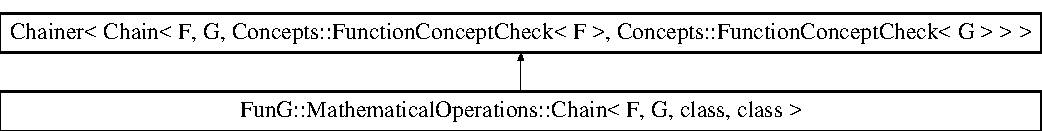
\includegraphics[height=1.078998cm]{structFunG_1_1MathematicalOperations_1_1Chain}
\end{center}
\end{figure}
\subsection*{Public Member Functions}
\begin{DoxyCompactItemize}
\item 
{\footnotesize template$<$class... Init\-Function$>$ }\\\hyperlink{structFunG_1_1MathematicalOperations_1_1Chain_a11bbc19be4ace14904de0be6d703fb1f}{Chain} (const Init\-Function \&...init)
\begin{DoxyCompactList}\small\item\em Constructor. \end{DoxyCompactList}\item 
\hyperlink{structFunG_1_1MathematicalOperations_1_1Chain_a3167b6304026eb0bd92e57d0dd0087e0}{Chain} (const F \&f\-\_\-, const G \&g\-\_\-)
\begin{DoxyCompactList}\small\item\em Constructor taking copies of the functions to be chained. \end{DoxyCompactList}\item 
\hypertarget{structFunG_1_1MathematicalOperations_1_1Chain_adb7f63859ef7dbdd08b0908c3a17794d}{{\footnotesize template$<$class Arg $>$ }\\void \hyperlink{structFunG_1_1MathematicalOperations_1_1Chain_adb7f63859ef7dbdd08b0908c3a17794d}{update} (const Arg \&x)}\label{structFunG_1_1MathematicalOperations_1_1Chain_adb7f63859ef7dbdd08b0908c3a17794d}

\begin{DoxyCompactList}\small\item\em Reset point of evaluation. \end{DoxyCompactList}\item 
\hypertarget{structFunG_1_1MathematicalOperations_1_1Chain_adf372d1f3b00903528740f3da6820b77}{{\footnotesize template$<$int index, class Arg $>$ }\\void \hyperlink{structFunG_1_1MathematicalOperations_1_1Chain_adf372d1f3b00903528740f3da6820b77}{update\-Variable} (const Arg \&x)}\label{structFunG_1_1MathematicalOperations_1_1Chain_adf372d1f3b00903528740f3da6820b77}

\begin{DoxyCompactList}\small\item\em Propagate call to \hyperlink{structFunG_1_1MathematicalOperations_1_1Chain_adf372d1f3b00903528740f3da6820b77}{update\-Variable()} to f and g. \end{DoxyCompactList}\item 
\hypertarget{structFunG_1_1MathematicalOperations_1_1Chain_abaced47a1bdc62dd6625caed1d11134c}{const auto \& \hyperlink{structFunG_1_1MathematicalOperations_1_1Chain_abaced47a1bdc62dd6625caed1d11134c}{d0} () const noexcept}\label{structFunG_1_1MathematicalOperations_1_1Chain_abaced47a1bdc62dd6625caed1d11134c}

\begin{DoxyCompactList}\small\item\em Function value. \end{DoxyCompactList}\item 
{\footnotesize template$<$int id, class Arg , class Indexed\-Arg  = Indexed\-Type$<$\-Arg,id$>$, class Indexed\-F\-Arg  = Indexed\-Type$<$\-F\-Arg,id$>$, class  = std\-::enable\-\_\-if\-\_\-t$<$ Compute\-Chain\-D1$<$ F , D1$<$\-G,\-Indexed\-Arg$>$ , Indexed\-F\-Arg $>$\-::present$>$$>$ }\\auto \hyperlink{structFunG_1_1MathematicalOperations_1_1Chain_adfe741dee89257258b39df846fd16cf7}{d1} (Arg const \&dx) const 
\begin{DoxyCompactList}\small\item\em First directional derivative. \end{DoxyCompactList}\item 
{\footnotesize template$<$int idx, int idy, class Arg\-X , class Arg\-Y , class Indexed\-Arg\-X  = Indexed\-Type$<$\-Arg\-X,idx$>$, class Indexed\-Arg\-Y  = Indexed\-Type$<$\-Arg\-Y,idy$>$, class Indexed\-F\-Arg\-X  = Indexed\-Type$<$\-F\-Arg,idx$>$, class Indexed\-F\-Arg\-Y  = Indexed\-Type$<$\-F\-Arg,idy$>$, class  = std\-::enable\-\_\-if\-\_\-t$<$ D2\-Lazy\-Type$<$\-Indexed\-Arg\-X,\-Indexed\-Arg\-Y,\-Indexed\-F\-Arg\-X,\-Indexed\-F\-Arg\-Y$>$\-::present $>$$>$ }\\auto \hyperlink{structFunG_1_1MathematicalOperations_1_1Chain_a0ab88c09299ce967583408f7f7dcd2bb}{d2} (Arg\-X const \&dx, Arg\-Y const \&dy) const 
\begin{DoxyCompactList}\small\item\em Second directional derivative. \end{DoxyCompactList}\item 
{\footnotesize template$<$int idx, int idy, int idz, class Arg\-X , class Arg\-Y , class Arg\-Z , class Indexed\-Arg\-X  = Indexed\-Type$<$\-Arg\-X,idx$>$, class Indexed\-Arg\-Y  = Indexed\-Type$<$\-Arg\-Y,idy$>$, class Indexed\-Arg\-Z  = Indexed\-Type$<$\-Arg\-Z,idz$>$, class Indexed\-F\-Arg\-X  = Indexed\-Type$<$\-F\-Arg,idx$>$, class Indexed\-F\-Arg\-Y  = Indexed\-Type$<$\-F\-Arg,idy$>$, class Indexed\-F\-Arg\-Z  = Indexed\-Type$<$\-F\-Arg,idz$>$, class  = std\-::enable\-\_\-if\-\_\-t$<$ D3\-Lazy\-Type$<$\-Indexed\-Arg\-X,\-Indexed\-Arg\-Y,\-Indexed\-Arg\-Z,\-Indexed\-F\-Arg\-X,\-Indexed\-F\-Arg\-Y,\-Indexed\-F\-Arg\-Z$>$\-::present $>$$>$ }\\auto \hyperlink{structFunG_1_1MathematicalOperations_1_1Chain_a17ac1618545b9d9bd2efa873b36cfbc7}{d3} (Arg\-X const \&dx, Arg\-Y const \&dy, Arg\-Z const \&dz) const 
\begin{DoxyCompactList}\small\item\em Third directional derivative. \end{DoxyCompactList}\end{DoxyCompactItemize}


\subsection{Detailed Description}
\subsubsection*{template$<$class F, class G, class = Function\-Concept\-Check$<$\-F$>$, class = Function\-Concept\-Check$<$\-G$>$$>$struct Fun\-G\-::\-Mathematical\-Operations\-::\-Chain$<$ F, G, class, class $>$}

Chain $ f\circ g $ of functions $f$ and $g$ of type F resp. G (F and G must satisfy the requirements of \hyperlink{structFunG_1_1Concepts_1_1FunctionConcept}{Concepts\-::\-Function\-Concept}). 

\subsection{Constructor \& Destructor Documentation}
\hypertarget{structFunG_1_1MathematicalOperations_1_1Chain_a11bbc19be4ace14904de0be6d703fb1f}{\index{Fun\-G\-::\-Mathematical\-Operations\-::\-Chain@{Fun\-G\-::\-Mathematical\-Operations\-::\-Chain}!Chain@{Chain}}
\index{Chain@{Chain}!FunG::MathematicalOperations::Chain@{Fun\-G\-::\-Mathematical\-Operations\-::\-Chain}}
\subsubsection[{Chain}]{\setlength{\rightskip}{0pt plus 5cm}template$<$class F, class G, class  = Function\-Concept\-Check$<$\-F$>$, class  = Function\-Concept\-Check$<$\-G$>$$>$ template$<$class... Init\-Function$>$ {\bf Fun\-G\-::\-Mathematical\-Operations\-::\-Chain}$<$ F, G, class, class $>$\-::{\bf Chain} (
\begin{DoxyParamCaption}
\item[{const Init\-Function \&...}]{init}
\end{DoxyParamCaption}
)\hspace{0.3cm}{\ttfamily [inline]}}}\label{structFunG_1_1MathematicalOperations_1_1Chain_a11bbc19be4ace14904de0be6d703fb1f}


Constructor. 


\begin{DoxyParams}{Parameters}
{\em init} & input for a constructor of G \\
\hline
\end{DoxyParams}
\hypertarget{structFunG_1_1MathematicalOperations_1_1Chain_a3167b6304026eb0bd92e57d0dd0087e0}{\index{Fun\-G\-::\-Mathematical\-Operations\-::\-Chain@{Fun\-G\-::\-Mathematical\-Operations\-::\-Chain}!Chain@{Chain}}
\index{Chain@{Chain}!FunG::MathematicalOperations::Chain@{Fun\-G\-::\-Mathematical\-Operations\-::\-Chain}}
\subsubsection[{Chain}]{\setlength{\rightskip}{0pt plus 5cm}template$<$class F, class G, class  = Function\-Concept\-Check$<$\-F$>$, class  = Function\-Concept\-Check$<$\-G$>$$>$ {\bf Fun\-G\-::\-Mathematical\-Operations\-::\-Chain}$<$ F, G, class, class $>$\-::{\bf Chain} (
\begin{DoxyParamCaption}
\item[{const F \&}]{f\-\_\-, }
\item[{const G \&}]{g\-\_\-}
\end{DoxyParamCaption}
)\hspace{0.3cm}{\ttfamily [inline]}}}\label{structFunG_1_1MathematicalOperations_1_1Chain_a3167b6304026eb0bd92e57d0dd0087e0}


Constructor taking copies of the functions to be chained. 


\begin{DoxyParams}{Parameters}
{\em f\-\_\-} & outer function \\
\hline
{\em g\-\_\-} & inner function \\
\hline
\end{DoxyParams}


\subsection{Member Function Documentation}
\hypertarget{structFunG_1_1MathematicalOperations_1_1Chain_adfe741dee89257258b39df846fd16cf7}{\index{Fun\-G\-::\-Mathematical\-Operations\-::\-Chain@{Fun\-G\-::\-Mathematical\-Operations\-::\-Chain}!d1@{d1}}
\index{d1@{d1}!FunG::MathematicalOperations::Chain@{Fun\-G\-::\-Mathematical\-Operations\-::\-Chain}}
\subsubsection[{d1}]{\setlength{\rightskip}{0pt plus 5cm}template$<$class F, class G, class  = Function\-Concept\-Check$<$\-F$>$, class  = Function\-Concept\-Check$<$\-G$>$$>$ template$<$int id, class Arg , class Indexed\-Arg  = Indexed\-Type$<$\-Arg,id$>$, class Indexed\-F\-Arg  = Indexed\-Type$<$\-F\-Arg,id$>$, class  = std\-::enable\-\_\-if\-\_\-t$<$ Compute\-Chain\-D1$<$ F , D1$<$\-G,\-Indexed\-Arg$>$ , Indexed\-F\-Arg $>$\-::present$>$$>$ auto {\bf Fun\-G\-::\-Mathematical\-Operations\-::\-Chain}$<$ F, G, class, class $>$\-::d1 (
\begin{DoxyParamCaption}
\item[{Arg const \&}]{dx}
\end{DoxyParamCaption}
) const\hspace{0.3cm}{\ttfamily [inline]}}}\label{structFunG_1_1MathematicalOperations_1_1Chain_adfe741dee89257258b39df846fd16cf7}


First directional derivative. 


\begin{DoxyParams}{Parameters}
{\em dx} & direction for which the derivative is computed \\
\hline
\end{DoxyParams}
\hypertarget{structFunG_1_1MathematicalOperations_1_1Chain_a0ab88c09299ce967583408f7f7dcd2bb}{\index{Fun\-G\-::\-Mathematical\-Operations\-::\-Chain@{Fun\-G\-::\-Mathematical\-Operations\-::\-Chain}!d2@{d2}}
\index{d2@{d2}!FunG::MathematicalOperations::Chain@{Fun\-G\-::\-Mathematical\-Operations\-::\-Chain}}
\subsubsection[{d2}]{\setlength{\rightskip}{0pt plus 5cm}template$<$class F, class G, class  = Function\-Concept\-Check$<$\-F$>$, class  = Function\-Concept\-Check$<$\-G$>$$>$ template$<$int idx, int idy, class Arg\-X , class Arg\-Y , class Indexed\-Arg\-X  = Indexed\-Type$<$\-Arg\-X,idx$>$, class Indexed\-Arg\-Y  = Indexed\-Type$<$\-Arg\-Y,idy$>$, class Indexed\-F\-Arg\-X  = Indexed\-Type$<$\-F\-Arg,idx$>$, class Indexed\-F\-Arg\-Y  = Indexed\-Type$<$\-F\-Arg,idy$>$, class  = std\-::enable\-\_\-if\-\_\-t$<$ D2\-Lazy\-Type$<$\-Indexed\-Arg\-X,\-Indexed\-Arg\-Y,\-Indexed\-F\-Arg\-X,\-Indexed\-F\-Arg\-Y$>$\-::present $>$$>$ auto {\bf Fun\-G\-::\-Mathematical\-Operations\-::\-Chain}$<$ F, G, class, class $>$\-::d2 (
\begin{DoxyParamCaption}
\item[{Arg\-X const \&}]{dx, }
\item[{Arg\-Y const \&}]{dy}
\end{DoxyParamCaption}
) const\hspace{0.3cm}{\ttfamily [inline]}}}\label{structFunG_1_1MathematicalOperations_1_1Chain_a0ab88c09299ce967583408f7f7dcd2bb}


Second directional derivative. 


\begin{DoxyParams}{Parameters}
{\em dx} & direction for which the derivative is computed \\
\hline
{\em dy} & direction for which the derivative is computed \\
\hline
\end{DoxyParams}
\hypertarget{structFunG_1_1MathematicalOperations_1_1Chain_a17ac1618545b9d9bd2efa873b36cfbc7}{\index{Fun\-G\-::\-Mathematical\-Operations\-::\-Chain@{Fun\-G\-::\-Mathematical\-Operations\-::\-Chain}!d3@{d3}}
\index{d3@{d3}!FunG::MathematicalOperations::Chain@{Fun\-G\-::\-Mathematical\-Operations\-::\-Chain}}
\subsubsection[{d3}]{\setlength{\rightskip}{0pt plus 5cm}template$<$class F, class G, class  = Function\-Concept\-Check$<$\-F$>$, class  = Function\-Concept\-Check$<$\-G$>$$>$ template$<$int idx, int idy, int idz, class Arg\-X , class Arg\-Y , class Arg\-Z , class Indexed\-Arg\-X  = Indexed\-Type$<$\-Arg\-X,idx$>$, class Indexed\-Arg\-Y  = Indexed\-Type$<$\-Arg\-Y,idy$>$, class Indexed\-Arg\-Z  = Indexed\-Type$<$\-Arg\-Z,idz$>$, class Indexed\-F\-Arg\-X  = Indexed\-Type$<$\-F\-Arg,idx$>$, class Indexed\-F\-Arg\-Y  = Indexed\-Type$<$\-F\-Arg,idy$>$, class Indexed\-F\-Arg\-Z  = Indexed\-Type$<$\-F\-Arg,idz$>$, class  = std\-::enable\-\_\-if\-\_\-t$<$ D3\-Lazy\-Type$<$\-Indexed\-Arg\-X,\-Indexed\-Arg\-Y,\-Indexed\-Arg\-Z,\-Indexed\-F\-Arg\-X,\-Indexed\-F\-Arg\-Y,\-Indexed\-F\-Arg\-Z$>$\-::present $>$$>$ auto {\bf Fun\-G\-::\-Mathematical\-Operations\-::\-Chain}$<$ F, G, class, class $>$\-::d3 (
\begin{DoxyParamCaption}
\item[{Arg\-X const \&}]{dx, }
\item[{Arg\-Y const \&}]{dy, }
\item[{Arg\-Z const \&}]{dz}
\end{DoxyParamCaption}
) const\hspace{0.3cm}{\ttfamily [inline]}}}\label{structFunG_1_1MathematicalOperations_1_1Chain_a17ac1618545b9d9bd2efa873b36cfbc7}


Third directional derivative. 


\begin{DoxyParams}{Parameters}
{\em dx} & direction for which the derivative is computed \\
\hline
{\em dy} & direction for which the derivative is computed \\
\hline
{\em dz} & direction for which the derivative is computed \\
\hline
\end{DoxyParams}


The documentation for this struct was generated from the following file\-:\begin{DoxyCompactItemize}
\item 
fung/mathematical\-\_\-operations/chain.\-hh\end{DoxyCompactItemize}

\hypertarget{structFunG_1_1Constant}{\section{Fun\-G\-:\-:Constant$<$ Type, class $>$ Struct Template Reference}
\label{structFunG_1_1Constant}\index{Fun\-G\-::\-Constant$<$ Type, class $>$@{Fun\-G\-::\-Constant$<$ Type, class $>$}}
}


Wrap a constant.  




{\ttfamily \#include $<$constant.\-hh$>$}

Inheritance diagram for Fun\-G\-:\-:Constant$<$ Type, class $>$\-:\begin{figure}[H]
\begin{center}
\leavevmode
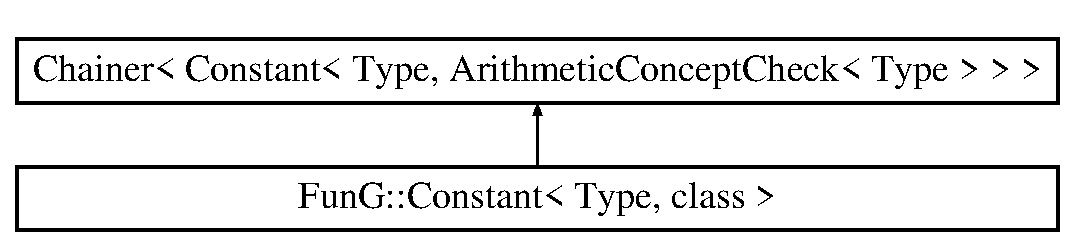
\includegraphics[height=2.000000cm]{structFunG_1_1Constant}
\end{center}
\end{figure}
\subsection*{Public Member Functions}
\begin{DoxyCompactItemize}
\item 
\hyperlink{structFunG_1_1Constant_a29ead8431e2fadfef397aae5dc5a4511}{Constant} ()=default
\item 
\hyperlink{structFunG_1_1Constant_aa01639e517f1224f3cbdc6b3542d8b97}{Constant} (Type t\-\_\-)
\begin{DoxyCompactList}\small\item\em Construct constant from copy. \end{DoxyCompactList}\item 
const Type \& \hyperlink{structFunG_1_1Constant_aad514a9470fbe1c47c0f07da6e160416}{d0} () const noexcept
\begin{DoxyCompactList}\small\item\em Function value. \end{DoxyCompactList}\end{DoxyCompactItemize}


\subsection{Detailed Description}
\subsubsection*{template$<$class Type, class = Arithmetic\-Concept\-Check$<$\-Type$>$$>$struct Fun\-G\-::\-Constant$<$ Type, class $>$}

Wrap a constant. 

\subsection{Constructor \& Destructor Documentation}
\hypertarget{structFunG_1_1Constant_a29ead8431e2fadfef397aae5dc5a4511}{\index{Fun\-G\-::\-Constant@{Fun\-G\-::\-Constant}!Constant@{Constant}}
\index{Constant@{Constant}!FunG::Constant@{Fun\-G\-::\-Constant}}
\subsubsection[{Constant}]{\setlength{\rightskip}{0pt plus 5cm}template$<$class Type , class  = Arithmetic\-Concept\-Check$<$\-Type$>$$>$ {\bf Fun\-G\-::\-Constant}$<$ Type, class $>$\-::{\bf Constant} (
\begin{DoxyParamCaption}
{}
\end{DoxyParamCaption}
)\hspace{0.3cm}{\ttfamily [default]}}}\label{structFunG_1_1Constant_a29ead8431e2fadfef397aae5dc5a4511}
\hypertarget{structFunG_1_1Constant_aa01639e517f1224f3cbdc6b3542d8b97}{\index{Fun\-G\-::\-Constant@{Fun\-G\-::\-Constant}!Constant@{Constant}}
\index{Constant@{Constant}!FunG::Constant@{Fun\-G\-::\-Constant}}
\subsubsection[{Constant}]{\setlength{\rightskip}{0pt plus 5cm}template$<$class Type , class  = Arithmetic\-Concept\-Check$<$\-Type$>$$>$ {\bf Fun\-G\-::\-Constant}$<$ Type, class $>$\-::{\bf Constant} (
\begin{DoxyParamCaption}
\item[{Type}]{t\-\_\-}
\end{DoxyParamCaption}
)\hspace{0.3cm}{\ttfamily [inline]}}}\label{structFunG_1_1Constant_aa01639e517f1224f3cbdc6b3542d8b97}


Construct constant from copy. 



\subsection{Member Function Documentation}
\hypertarget{structFunG_1_1Constant_aad514a9470fbe1c47c0f07da6e160416}{\index{Fun\-G\-::\-Constant@{Fun\-G\-::\-Constant}!d0@{d0}}
\index{d0@{d0}!FunG::Constant@{Fun\-G\-::\-Constant}}
\subsubsection[{d0}]{\setlength{\rightskip}{0pt plus 5cm}template$<$class Type , class  = Arithmetic\-Concept\-Check$<$\-Type$>$$>$ const Type\& {\bf Fun\-G\-::\-Constant}$<$ Type, class $>$\-::d0 (
\begin{DoxyParamCaption}
{}
\end{DoxyParamCaption}
) const\hspace{0.3cm}{\ttfamily [inline]}, {\ttfamily [noexcept]}}}\label{structFunG_1_1Constant_aad514a9470fbe1c47c0f07da6e160416}


Function value. 



The documentation for this struct was generated from the following file\-:\begin{DoxyCompactItemize}
\item 
fung/\hyperlink{constant_8hh}{constant.\-hh}\end{DoxyCompactItemize}

\hypertarget{structFunG_1_1Concepts_1_1CopyConcept}{\section{Fun\-G\-:\-:Concepts\-:\-:Copy\-Concept Struct Reference}
\label{structFunG_1_1Concepts_1_1CopyConcept}\index{Fun\-G\-::\-Concepts\-::\-Copy\-Concept@{Fun\-G\-::\-Concepts\-::\-Copy\-Concept}}
}


Requires copy-\/constructibility and copy-\/assignability.  




{\ttfamily \#include $<$concepts.\-hh$>$}

Inheritance diagram for Fun\-G\-:\-:Concepts\-:\-:Copy\-Concept\-:\begin{figure}[H]
\begin{center}
\leavevmode
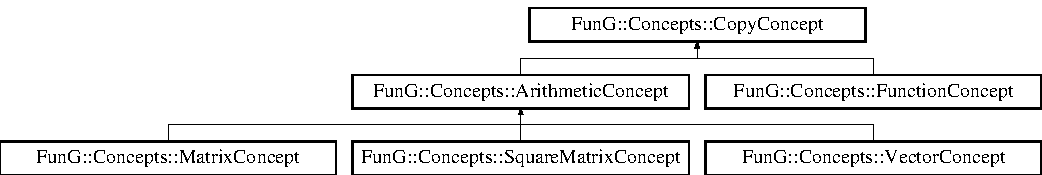
\includegraphics[height=2.352941cm]{structFunG_1_1Concepts_1_1CopyConcept}
\end{center}
\end{figure}
\subsection*{Public Member Functions}
\begin{DoxyCompactItemize}
\item 
\hypertarget{structFunG_1_1Concepts_1_1CopyConcept_afc08741d422ff46c2e681efc38913144}{\hyperlink{structFunG_1_1Concepts_1_1CopyConcept_afc08741d422ff46c2e681efc38913144}{Copy\-Concept} (const \hyperlink{structFunG_1_1Concepts_1_1CopyConcept}{Copy\-Concept} \&)}\label{structFunG_1_1Concepts_1_1CopyConcept_afc08741d422ff46c2e681efc38913144}

\begin{DoxyCompactList}\small\item\em Copy-\/constructible. \end{DoxyCompactList}\item 
\hypertarget{structFunG_1_1Concepts_1_1CopyConcept_a43c6c112f8164497a4279458af2c0b20}{\hyperlink{structFunG_1_1Concepts_1_1CopyConcept}{Copy\-Concept} \& \hyperlink{structFunG_1_1Concepts_1_1CopyConcept_a43c6c112f8164497a4279458af2c0b20}{operator=} (const \hyperlink{structFunG_1_1Concepts_1_1CopyConcept}{Copy\-Concept} \&)}\label{structFunG_1_1Concepts_1_1CopyConcept_a43c6c112f8164497a4279458af2c0b20}

\begin{DoxyCompactList}\small\item\em Copy-\/assignable. \end{DoxyCompactList}\end{DoxyCompactItemize}


\subsection{Detailed Description}
Requires copy-\/constructibility and copy-\/assignability. 

The documentation for this struct was generated from the following file\-:\begin{DoxyCompactItemize}
\item 
fung/\hyperlink{concepts_8hh}{concepts.\-hh}\end{DoxyCompactItemize}

\hypertarget{structFunG_1_1Concepts_1_1CopyConceptCheck}{\section{Fun\-G\-:\-:Concepts\-:\-:Copy\-Concept\-Check$<$ Arg $>$ Struct Template Reference}
\label{structFunG_1_1Concepts_1_1CopyConceptCheck}\index{Fun\-G\-::\-Concepts\-::\-Copy\-Concept\-Check$<$ Arg $>$@{Fun\-G\-::\-Concepts\-::\-Copy\-Concept\-Check$<$ Arg $>$}}
}


Static check if the requirements of \hyperlink{structFunG_1_1Concepts_1_1CopyConcept}{Copy\-Concept} are satisfied.  




{\ttfamily \#include $<$concept\-Check.\-hh$>$}

Inheritance diagram for Fun\-G\-:\-:Concepts\-:\-:Copy\-Concept\-Check$<$ Arg $>$\-:\begin{figure}[H]
\begin{center}
\leavevmode
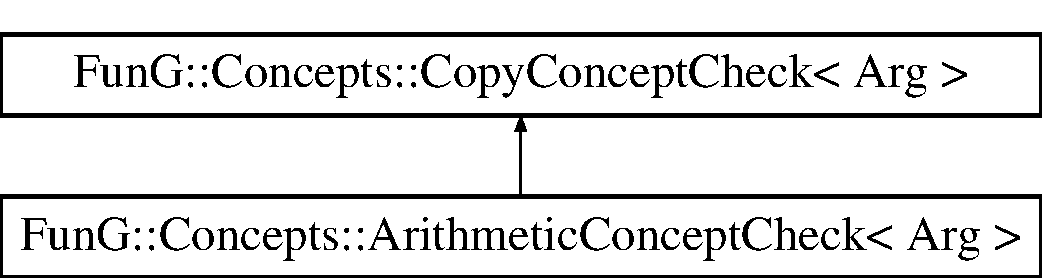
\includegraphics[height=2.000000cm]{structFunG_1_1Concepts_1_1CopyConceptCheck}
\end{center}
\end{figure}


\subsection{Detailed Description}
\subsubsection*{template$<$class Arg$>$struct Fun\-G\-::\-Concepts\-::\-Copy\-Concept\-Check$<$ Arg $>$}

Static check if the requirements of \hyperlink{structFunG_1_1Concepts_1_1CopyConcept}{Copy\-Concept} are satisfied. 


\begin{DoxyTemplParams}{Template Parameters}
{\em Arg} & type to check \\
\hline
\end{DoxyTemplParams}


The documentation for this struct was generated from the following file\-:\begin{DoxyCompactItemize}
\item 
Fun\-G/concept\-Check.\-hh\end{DoxyCompactItemize}

\hypertarget{structFunG_1_1Cos}{\section{Fun\-G\-:\-:Cos Struct Reference}
\label{structFunG_1_1Cos}\index{Fun\-G\-::\-Cos@{Fun\-G\-::\-Cos}}
}


Cosine function including first three derivatives (based on cos(double) in $<$cmath$>$).  




{\ttfamily \#include $<$cosine.\-hh$>$}

Inheritance diagram for Fun\-G\-:\-:Cos\-:\begin{figure}[H]
\begin{center}
\leavevmode
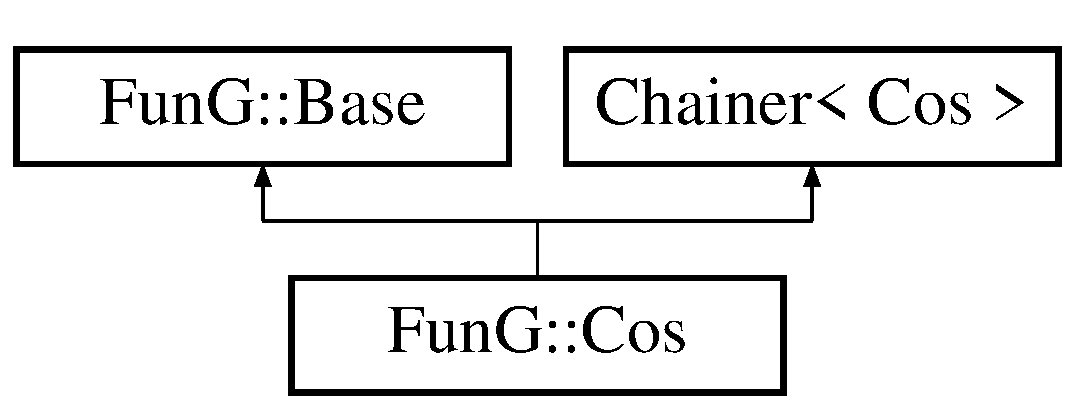
\includegraphics[height=2.000000cm]{structFunG_1_1Cos}
\end{center}
\end{figure}
\subsection*{Public Member Functions}
\begin{DoxyCompactItemize}
\item 
constexpr \hyperlink{structFunG_1_1Cos_a40c049c8842e387ccc5ab5f3720c938e}{Cos} (double x=0.)
\begin{DoxyCompactList}\small\item\em Constructor. \end{DoxyCompactList}\item 
void \hyperlink{structFunG_1_1Cos_a502c2a5f9f7e055e00192d185a5a0a50}{update} (const double \&x)
\begin{DoxyCompactList}\small\item\em Set point of evaluation. \end{DoxyCompactList}\item 
double \hyperlink{structFunG_1_1Cos_af1391a01b4031ebeb9a2db8127486127}{d0} () const noexcept
\begin{DoxyCompactList}\small\item\em Function value. \end{DoxyCompactList}\item 
double \hyperlink{structFunG_1_1Cos_a0d3494ce7fda10e3f64a2790d64c3b31}{d1} (double dx=1.) const 
\begin{DoxyCompactList}\small\item\em First (directional) derivative. \end{DoxyCompactList}\item 
double \hyperlink{structFunG_1_1Cos_ad48e6be302369c1fefbe29687823a617}{d2} (double dx=1., double dy=1.) const 
\begin{DoxyCompactList}\small\item\em Second (directional) derivative. \end{DoxyCompactList}\item 
double \hyperlink{structFunG_1_1Cos_abda328f29bee29f2af535c5f307de9c8}{d3} (double dx=1., double dy=1., double dz=1.) const 
\begin{DoxyCompactList}\small\item\em Third (directional) derivative. \end{DoxyCompactList}\end{DoxyCompactItemize}


\subsection{Detailed Description}
Cosine function including first three derivatives (based on cos(double) in $<$cmath$>$). 

For scalar functions directional derivatives are less interesting. Incorporating this function as building block for more complex functions requires directional derivatives. These occur during applications of the chain rule. 

\subsection{Constructor \& Destructor Documentation}
\hypertarget{structFunG_1_1Cos_a40c049c8842e387ccc5ab5f3720c938e}{\index{Fun\-G\-::\-Cos@{Fun\-G\-::\-Cos}!Cos@{Cos}}
\index{Cos@{Cos}!FunG::Cos@{Fun\-G\-::\-Cos}}
\subsubsection[{Cos}]{\setlength{\rightskip}{0pt plus 5cm}constexpr Fun\-G\-::\-Cos\-::\-Cos (
\begin{DoxyParamCaption}
\item[{double}]{x = {\ttfamily 0.}}
\end{DoxyParamCaption}
)\hspace{0.3cm}{\ttfamily [inline]}, {\ttfamily [explicit]}}}\label{structFunG_1_1Cos_a40c049c8842e387ccc5ab5f3720c938e}


Constructor. 


\begin{DoxyParams}{Parameters}
{\em x} & point of evaluation \\
\hline
\end{DoxyParams}


\subsection{Member Function Documentation}
\hypertarget{structFunG_1_1Cos_af1391a01b4031ebeb9a2db8127486127}{\index{Fun\-G\-::\-Cos@{Fun\-G\-::\-Cos}!d0@{d0}}
\index{d0@{d0}!FunG::Cos@{Fun\-G\-::\-Cos}}
\subsubsection[{d0}]{\setlength{\rightskip}{0pt plus 5cm}double Fun\-G\-::\-Cos\-::d0 (
\begin{DoxyParamCaption}
{}
\end{DoxyParamCaption}
) const\hspace{0.3cm}{\ttfamily [inline]}, {\ttfamily [noexcept]}}}\label{structFunG_1_1Cos_af1391a01b4031ebeb9a2db8127486127}


Function value. 

\hypertarget{structFunG_1_1Cos_a0d3494ce7fda10e3f64a2790d64c3b31}{\index{Fun\-G\-::\-Cos@{Fun\-G\-::\-Cos}!d1@{d1}}
\index{d1@{d1}!FunG::Cos@{Fun\-G\-::\-Cos}}
\subsubsection[{d1}]{\setlength{\rightskip}{0pt plus 5cm}double Fun\-G\-::\-Cos\-::d1 (
\begin{DoxyParamCaption}
\item[{double}]{dx = {\ttfamily 1.}}
\end{DoxyParamCaption}
) const\hspace{0.3cm}{\ttfamily [inline]}}}\label{structFunG_1_1Cos_a0d3494ce7fda10e3f64a2790d64c3b31}


First (directional) derivative. 

\hypertarget{structFunG_1_1Cos_ad48e6be302369c1fefbe29687823a617}{\index{Fun\-G\-::\-Cos@{Fun\-G\-::\-Cos}!d2@{d2}}
\index{d2@{d2}!FunG::Cos@{Fun\-G\-::\-Cos}}
\subsubsection[{d2}]{\setlength{\rightskip}{0pt plus 5cm}double Fun\-G\-::\-Cos\-::d2 (
\begin{DoxyParamCaption}
\item[{double}]{dx = {\ttfamily 1.}, }
\item[{double}]{dy = {\ttfamily 1.}}
\end{DoxyParamCaption}
) const\hspace{0.3cm}{\ttfamily [inline]}}}\label{structFunG_1_1Cos_ad48e6be302369c1fefbe29687823a617}


Second (directional) derivative. 

\hypertarget{structFunG_1_1Cos_abda328f29bee29f2af535c5f307de9c8}{\index{Fun\-G\-::\-Cos@{Fun\-G\-::\-Cos}!d3@{d3}}
\index{d3@{d3}!FunG::Cos@{Fun\-G\-::\-Cos}}
\subsubsection[{d3}]{\setlength{\rightskip}{0pt plus 5cm}double Fun\-G\-::\-Cos\-::d3 (
\begin{DoxyParamCaption}
\item[{double}]{dx = {\ttfamily 1.}, }
\item[{double}]{dy = {\ttfamily 1.}, }
\item[{double}]{dz = {\ttfamily 1.}}
\end{DoxyParamCaption}
) const\hspace{0.3cm}{\ttfamily [inline]}}}\label{structFunG_1_1Cos_abda328f29bee29f2af535c5f307de9c8}


Third (directional) derivative. 

\hypertarget{structFunG_1_1Cos_a502c2a5f9f7e055e00192d185a5a0a50}{\index{Fun\-G\-::\-Cos@{Fun\-G\-::\-Cos}!update@{update}}
\index{update@{update}!FunG::Cos@{Fun\-G\-::\-Cos}}
\subsubsection[{update}]{\setlength{\rightskip}{0pt plus 5cm}void Fun\-G\-::\-Cos\-::update (
\begin{DoxyParamCaption}
\item[{const double \&}]{x}
\end{DoxyParamCaption}
)\hspace{0.3cm}{\ttfamily [inline]}}}\label{structFunG_1_1Cos_a502c2a5f9f7e055e00192d185a5a0a50}


Set point of evaluation. 



The documentation for this struct was generated from the following file\-:\begin{DoxyCompactItemize}
\item 
include/fung/cmath/\hyperlink{cmath_2cosine_8hh}{cosine.\-hh}\end{DoxyCompactItemize}

\hypertarget{structFunG_1_1texify_1_1Cos}{\section{Fun\-G\-:\-:texify\-:\-:Cos Struct Reference}
\label{structFunG_1_1texify_1_1Cos}\index{Fun\-G\-::texify\-::\-Cos@{Fun\-G\-::texify\-::\-Cos}}
}


{\ttfamily \#include $<$cosine.\-hh$>$}

Inheritance diagram for Fun\-G\-:\-:texify\-:\-:Cos\-:\begin{figure}[H]
\begin{center}
\leavevmode
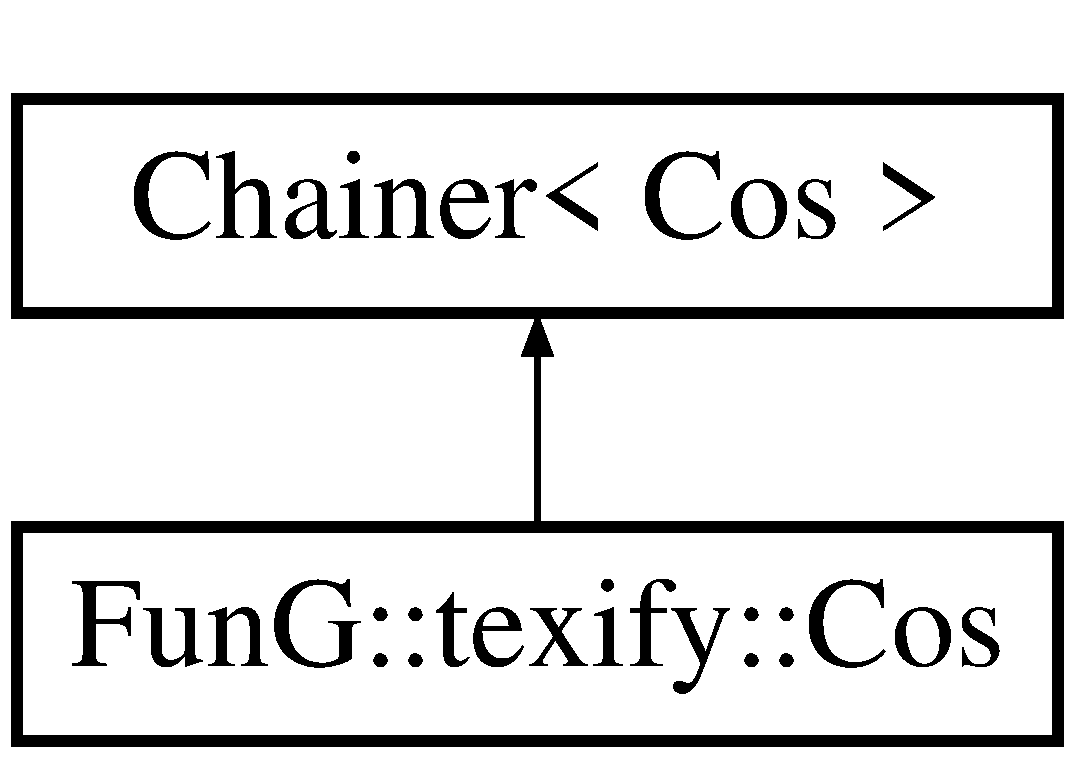
\includegraphics[height=2.000000cm]{structFunG_1_1texify_1_1Cos}
\end{center}
\end{figure}
\subsection*{Public Member Functions}
\begin{DoxyCompactItemize}
\item 
\hyperlink{structFunG_1_1texify_1_1Cos_afa8ef16bb63bf84ed292cf570a51fe43}{Cos} (std\-::string x=\char`\"{}x\char`\"{})
\begin{DoxyCompactList}\small\item\em Constructor. \end{DoxyCompactList}\item 
void \hyperlink{structFunG_1_1texify_1_1Cos_a72a69fddcac8cfd95da506b8f601c383}{update} (const std\-::string \&x)
\begin{DoxyCompactList}\small\item\em Set point of evaluation. \end{DoxyCompactList}\item 
std\-::string \hyperlink{structFunG_1_1texify_1_1Cos_a52e954aa7573562dfc424cd5b843080c}{d0} () const noexcept
\begin{DoxyCompactList}\small\item\em Function value. \end{DoxyCompactList}\item 
std\-::string \hyperlink{structFunG_1_1texify_1_1Cos_ae286506ec155649738ed8d43cb99844d}{d1} (const std\-::string \&dx=\char`\"{}\char`\"{}) const 
\begin{DoxyCompactList}\small\item\em First (directional) derivative. \end{DoxyCompactList}\item 
std\-::string \hyperlink{structFunG_1_1texify_1_1Cos_a27b2fd25de2226972db306db4611e3fd}{d2} (const std\-::string \&dx=\char`\"{}\char`\"{}, const std\-::string \&dy=\char`\"{}\char`\"{}) const 
\begin{DoxyCompactList}\small\item\em Second (directional) derivative. \end{DoxyCompactList}\item 
std\-::string \hyperlink{structFunG_1_1texify_1_1Cos_a017da65281e3c4862990d71788c4929c}{d3} (const std\-::string \&dx=\char`\"{}\char`\"{}, const std\-::string \&dy=\char`\"{}\char`\"{}, const std\-::string \&dz=\char`\"{}\char`\"{}) const 
\begin{DoxyCompactList}\small\item\em Third (directional) derivative. \end{DoxyCompactList}\end{DoxyCompactItemize}


\subsection{Constructor \& Destructor Documentation}
\hypertarget{structFunG_1_1texify_1_1Cos_afa8ef16bb63bf84ed292cf570a51fe43}{\index{Fun\-G\-::texify\-::\-Cos@{Fun\-G\-::texify\-::\-Cos}!Cos@{Cos}}
\index{Cos@{Cos}!FunG::texify::Cos@{Fun\-G\-::texify\-::\-Cos}}
\subsubsection[{Cos}]{\setlength{\rightskip}{0pt plus 5cm}Fun\-G\-::texify\-::\-Cos\-::\-Cos (
\begin{DoxyParamCaption}
\item[{std\-::string}]{x = {\ttfamily \char`\"{}x\char`\"{}}}
\end{DoxyParamCaption}
)\hspace{0.3cm}{\ttfamily [inline]}, {\ttfamily [explicit]}}}\label{structFunG_1_1texify_1_1Cos_afa8ef16bb63bf84ed292cf570a51fe43}


Constructor. 


\begin{DoxyParams}{Parameters}
{\em x} & point of evaluation \\
\hline
\end{DoxyParams}


\subsection{Member Function Documentation}
\hypertarget{structFunG_1_1texify_1_1Cos_a52e954aa7573562dfc424cd5b843080c}{\index{Fun\-G\-::texify\-::\-Cos@{Fun\-G\-::texify\-::\-Cos}!d0@{d0}}
\index{d0@{d0}!FunG::texify::Cos@{Fun\-G\-::texify\-::\-Cos}}
\subsubsection[{d0}]{\setlength{\rightskip}{0pt plus 5cm}std\-::string Fun\-G\-::texify\-::\-Cos\-::d0 (
\begin{DoxyParamCaption}
{}
\end{DoxyParamCaption}
) const\hspace{0.3cm}{\ttfamily [inline]}, {\ttfamily [noexcept]}}}\label{structFunG_1_1texify_1_1Cos_a52e954aa7573562dfc424cd5b843080c}


Function value. 

\hypertarget{structFunG_1_1texify_1_1Cos_ae286506ec155649738ed8d43cb99844d}{\index{Fun\-G\-::texify\-::\-Cos@{Fun\-G\-::texify\-::\-Cos}!d1@{d1}}
\index{d1@{d1}!FunG::texify::Cos@{Fun\-G\-::texify\-::\-Cos}}
\subsubsection[{d1}]{\setlength{\rightskip}{0pt plus 5cm}std\-::string Fun\-G\-::texify\-::\-Cos\-::d1 (
\begin{DoxyParamCaption}
\item[{const std\-::string \&}]{dx = {\ttfamily \char`\"{}\char`\"{}}}
\end{DoxyParamCaption}
) const\hspace{0.3cm}{\ttfamily [inline]}}}\label{structFunG_1_1texify_1_1Cos_ae286506ec155649738ed8d43cb99844d}


First (directional) derivative. 

\hypertarget{structFunG_1_1texify_1_1Cos_a27b2fd25de2226972db306db4611e3fd}{\index{Fun\-G\-::texify\-::\-Cos@{Fun\-G\-::texify\-::\-Cos}!d2@{d2}}
\index{d2@{d2}!FunG::texify::Cos@{Fun\-G\-::texify\-::\-Cos}}
\subsubsection[{d2}]{\setlength{\rightskip}{0pt plus 5cm}std\-::string Fun\-G\-::texify\-::\-Cos\-::d2 (
\begin{DoxyParamCaption}
\item[{const std\-::string \&}]{dx = {\ttfamily \char`\"{}\char`\"{}}, }
\item[{const std\-::string \&}]{dy = {\ttfamily \char`\"{}\char`\"{}}}
\end{DoxyParamCaption}
) const\hspace{0.3cm}{\ttfamily [inline]}}}\label{structFunG_1_1texify_1_1Cos_a27b2fd25de2226972db306db4611e3fd}


Second (directional) derivative. 

\hypertarget{structFunG_1_1texify_1_1Cos_a017da65281e3c4862990d71788c4929c}{\index{Fun\-G\-::texify\-::\-Cos@{Fun\-G\-::texify\-::\-Cos}!d3@{d3}}
\index{d3@{d3}!FunG::texify::Cos@{Fun\-G\-::texify\-::\-Cos}}
\subsubsection[{d3}]{\setlength{\rightskip}{0pt plus 5cm}std\-::string Fun\-G\-::texify\-::\-Cos\-::d3 (
\begin{DoxyParamCaption}
\item[{const std\-::string \&}]{dx = {\ttfamily \char`\"{}\char`\"{}}, }
\item[{const std\-::string \&}]{dy = {\ttfamily \char`\"{}\char`\"{}}, }
\item[{const std\-::string \&}]{dz = {\ttfamily \char`\"{}\char`\"{}}}
\end{DoxyParamCaption}
) const\hspace{0.3cm}{\ttfamily [inline]}}}\label{structFunG_1_1texify_1_1Cos_a017da65281e3c4862990d71788c4929c}


Third (directional) derivative. 

\hypertarget{structFunG_1_1texify_1_1Cos_a72a69fddcac8cfd95da506b8f601c383}{\index{Fun\-G\-::texify\-::\-Cos@{Fun\-G\-::texify\-::\-Cos}!update@{update}}
\index{update@{update}!FunG::texify::Cos@{Fun\-G\-::texify\-::\-Cos}}
\subsubsection[{update}]{\setlength{\rightskip}{0pt plus 5cm}void Fun\-G\-::texify\-::\-Cos\-::update (
\begin{DoxyParamCaption}
\item[{const std\-::string \&}]{x}
\end{DoxyParamCaption}
)\hspace{0.3cm}{\ttfamily [inline]}}}\label{structFunG_1_1texify_1_1Cos_a72a69fddcac8cfd95da506b8f601c383}


Set point of evaluation. 



The documentation for this struct was generated from the following file\-:\begin{DoxyCompactItemize}
\item 
include/fung/texify/cmath/\hyperlink{texify_2cmath_2cosine_8hh}{cosine.\-hh}\end{DoxyCompactItemize}

\hypertarget{structFunG_1_1stringify_1_1Cos}{\section{Fun\-G\-:\-:stringify\-:\-:Cos Struct Reference}
\label{structFunG_1_1stringify_1_1Cos}\index{Fun\-G\-::stringify\-::\-Cos@{Fun\-G\-::stringify\-::\-Cos}}
}


{\ttfamily \#include $<$cosine.\-hh$>$}

Inheritance diagram for Fun\-G\-:\-:stringify\-:\-:Cos\-:\begin{figure}[H]
\begin{center}
\leavevmode
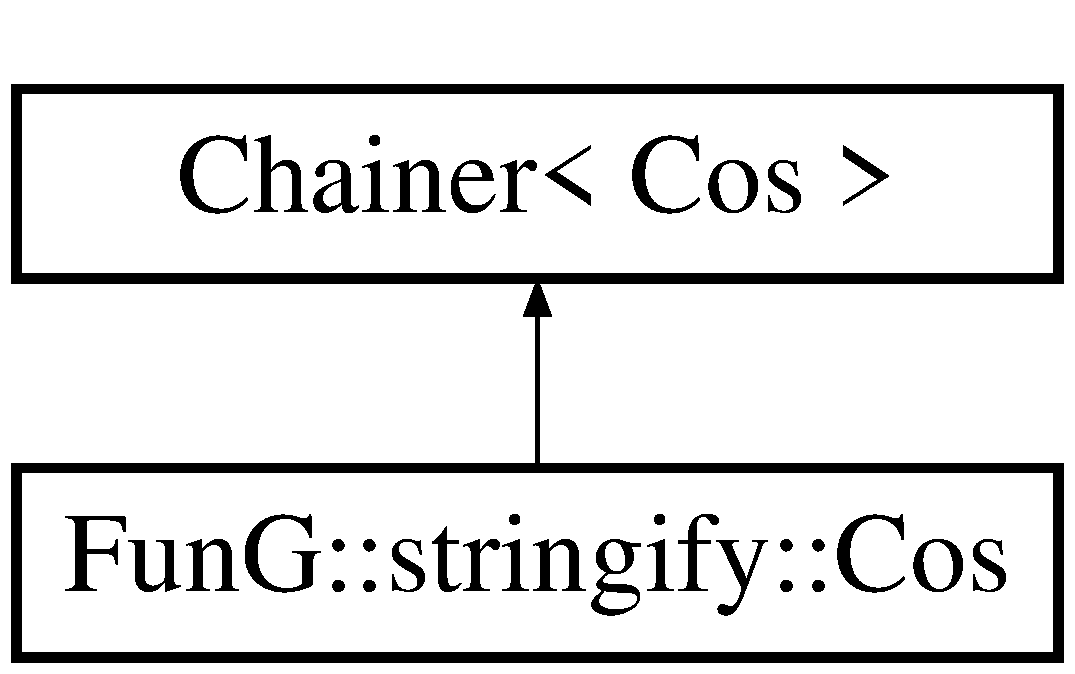
\includegraphics[height=2.000000cm]{structFunG_1_1stringify_1_1Cos}
\end{center}
\end{figure}
\subsection*{Public Member Functions}
\begin{DoxyCompactItemize}
\item 
\hyperlink{structFunG_1_1stringify_1_1Cos_a9069519fc6a176ae47f9b70a29da2e44}{Cos} (std\-::string x=\char`\"{}x\char`\"{})
\begin{DoxyCompactList}\small\item\em Constructor. \end{DoxyCompactList}\item 
void \hyperlink{structFunG_1_1stringify_1_1Cos_a3f0de2f0759f6b680eca1a844d0c4dde}{update} (const std\-::string \&x)
\begin{DoxyCompactList}\small\item\em Set point of evaluation. \end{DoxyCompactList}\item 
std\-::string \hyperlink{structFunG_1_1stringify_1_1Cos_aba8c4e517e67faca4b20814a5765070a}{d0} () const noexcept
\begin{DoxyCompactList}\small\item\em Function value. \end{DoxyCompactList}\item 
std\-::string \hyperlink{structFunG_1_1stringify_1_1Cos_a0529aa1639af25cd28cd2e2e0b671466}{d1} (const std\-::string \&dx=\char`\"{}\char`\"{}) const 
\begin{DoxyCompactList}\small\item\em First (directional) derivative. \end{DoxyCompactList}\item 
std\-::string \hyperlink{structFunG_1_1stringify_1_1Cos_a771b19e97e2fc910b24fbcc0f806bdd3}{d2} (const std\-::string \&dx=\char`\"{}\char`\"{}, const std\-::string \&dy=\char`\"{}\char`\"{}) const 
\begin{DoxyCompactList}\small\item\em Second (directional) derivative. \end{DoxyCompactList}\item 
std\-::string \hyperlink{structFunG_1_1stringify_1_1Cos_ad6f265f296b7cf2da1f5a9ecfc98598e}{d3} (const std\-::string \&dx=\char`\"{}\char`\"{}, const std\-::string \&dy=\char`\"{}\char`\"{}, const std\-::string \&dz=\char`\"{}\char`\"{}) const 
\begin{DoxyCompactList}\small\item\em Third (directional) derivative. \end{DoxyCompactList}\end{DoxyCompactItemize}


\subsection{Constructor \& Destructor Documentation}
\hypertarget{structFunG_1_1stringify_1_1Cos_a9069519fc6a176ae47f9b70a29da2e44}{\index{Fun\-G\-::stringify\-::\-Cos@{Fun\-G\-::stringify\-::\-Cos}!Cos@{Cos}}
\index{Cos@{Cos}!FunG::stringify::Cos@{Fun\-G\-::stringify\-::\-Cos}}
\subsubsection[{Cos}]{\setlength{\rightskip}{0pt plus 5cm}Fun\-G\-::stringify\-::\-Cos\-::\-Cos (
\begin{DoxyParamCaption}
\item[{std\-::string}]{x = {\ttfamily \char`\"{}x\char`\"{}}}
\end{DoxyParamCaption}
)\hspace{0.3cm}{\ttfamily [inline]}, {\ttfamily [explicit]}}}\label{structFunG_1_1stringify_1_1Cos_a9069519fc6a176ae47f9b70a29da2e44}


Constructor. 


\begin{DoxyParams}{Parameters}
{\em x} & point of evaluation \\
\hline
\end{DoxyParams}


\subsection{Member Function Documentation}
\hypertarget{structFunG_1_1stringify_1_1Cos_aba8c4e517e67faca4b20814a5765070a}{\index{Fun\-G\-::stringify\-::\-Cos@{Fun\-G\-::stringify\-::\-Cos}!d0@{d0}}
\index{d0@{d0}!FunG::stringify::Cos@{Fun\-G\-::stringify\-::\-Cos}}
\subsubsection[{d0}]{\setlength{\rightskip}{0pt plus 5cm}std\-::string Fun\-G\-::stringify\-::\-Cos\-::d0 (
\begin{DoxyParamCaption}
{}
\end{DoxyParamCaption}
) const\hspace{0.3cm}{\ttfamily [inline]}, {\ttfamily [noexcept]}}}\label{structFunG_1_1stringify_1_1Cos_aba8c4e517e67faca4b20814a5765070a}


Function value. 

\hypertarget{structFunG_1_1stringify_1_1Cos_a0529aa1639af25cd28cd2e2e0b671466}{\index{Fun\-G\-::stringify\-::\-Cos@{Fun\-G\-::stringify\-::\-Cos}!d1@{d1}}
\index{d1@{d1}!FunG::stringify::Cos@{Fun\-G\-::stringify\-::\-Cos}}
\subsubsection[{d1}]{\setlength{\rightskip}{0pt plus 5cm}std\-::string Fun\-G\-::stringify\-::\-Cos\-::d1 (
\begin{DoxyParamCaption}
\item[{const std\-::string \&}]{dx = {\ttfamily \char`\"{}\char`\"{}}}
\end{DoxyParamCaption}
) const\hspace{0.3cm}{\ttfamily [inline]}}}\label{structFunG_1_1stringify_1_1Cos_a0529aa1639af25cd28cd2e2e0b671466}


First (directional) derivative. 

\hypertarget{structFunG_1_1stringify_1_1Cos_a771b19e97e2fc910b24fbcc0f806bdd3}{\index{Fun\-G\-::stringify\-::\-Cos@{Fun\-G\-::stringify\-::\-Cos}!d2@{d2}}
\index{d2@{d2}!FunG::stringify::Cos@{Fun\-G\-::stringify\-::\-Cos}}
\subsubsection[{d2}]{\setlength{\rightskip}{0pt plus 5cm}std\-::string Fun\-G\-::stringify\-::\-Cos\-::d2 (
\begin{DoxyParamCaption}
\item[{const std\-::string \&}]{dx = {\ttfamily \char`\"{}\char`\"{}}, }
\item[{const std\-::string \&}]{dy = {\ttfamily \char`\"{}\char`\"{}}}
\end{DoxyParamCaption}
) const\hspace{0.3cm}{\ttfamily [inline]}}}\label{structFunG_1_1stringify_1_1Cos_a771b19e97e2fc910b24fbcc0f806bdd3}


Second (directional) derivative. 

\hypertarget{structFunG_1_1stringify_1_1Cos_ad6f265f296b7cf2da1f5a9ecfc98598e}{\index{Fun\-G\-::stringify\-::\-Cos@{Fun\-G\-::stringify\-::\-Cos}!d3@{d3}}
\index{d3@{d3}!FunG::stringify::Cos@{Fun\-G\-::stringify\-::\-Cos}}
\subsubsection[{d3}]{\setlength{\rightskip}{0pt plus 5cm}std\-::string Fun\-G\-::stringify\-::\-Cos\-::d3 (
\begin{DoxyParamCaption}
\item[{const std\-::string \&}]{dx = {\ttfamily \char`\"{}\char`\"{}}, }
\item[{const std\-::string \&}]{dy = {\ttfamily \char`\"{}\char`\"{}}, }
\item[{const std\-::string \&}]{dz = {\ttfamily \char`\"{}\char`\"{}}}
\end{DoxyParamCaption}
) const\hspace{0.3cm}{\ttfamily [inline]}}}\label{structFunG_1_1stringify_1_1Cos_ad6f265f296b7cf2da1f5a9ecfc98598e}


Third (directional) derivative. 

\hypertarget{structFunG_1_1stringify_1_1Cos_a3f0de2f0759f6b680eca1a844d0c4dde}{\index{Fun\-G\-::stringify\-::\-Cos@{Fun\-G\-::stringify\-::\-Cos}!update@{update}}
\index{update@{update}!FunG::stringify::Cos@{Fun\-G\-::stringify\-::\-Cos}}
\subsubsection[{update}]{\setlength{\rightskip}{0pt plus 5cm}void Fun\-G\-::stringify\-::\-Cos\-::update (
\begin{DoxyParamCaption}
\item[{const std\-::string \&}]{x}
\end{DoxyParamCaption}
)\hspace{0.3cm}{\ttfamily [inline]}}}\label{structFunG_1_1stringify_1_1Cos_a3f0de2f0759f6b680eca1a844d0c4dde}


Set point of evaluation. 



The documentation for this struct was generated from the following file\-:\begin{DoxyCompactItemize}
\item 
include/fung/cmath/stringify/\hyperlink{stringify_2cosine_8hh}{cosine.\-hh}\end{DoxyCompactItemize}

\hypertarget{structFunG_1_1Decay}{\section{Fun\-G\-:\-:Decay$<$ F, class $>$ Struct Template Reference}
\label{structFunG_1_1Decay}\index{Fun\-G\-::\-Decay$<$ F, class $>$@{Fun\-G\-::\-Decay$<$ F, class $>$}}
}


Identity, i.\-e. \hyperlink{structFunG_1_1Decay_a4b2916cbb7c8587ab3fccc9b896b9df4}{Decay$<$\-F$>$\-::type} == F  




{\ttfamily \#include $<$type\-\_\-traits.\-hh$>$}

\subsection*{Public Types}
\begin{DoxyCompactItemize}
\item 
using \hyperlink{structFunG_1_1Decay_a4b2916cbb7c8587ab3fccc9b896b9df4}{type} = F
\end{DoxyCompactItemize}


\subsection{Detailed Description}
\subsubsection*{template$<$class F, class = void$>$struct Fun\-G\-::\-Decay$<$ F, class $>$}

Identity, i.\-e. \hyperlink{structFunG_1_1Decay_a4b2916cbb7c8587ab3fccc9b896b9df4}{Decay$<$\-F$>$\-::type} == F 

\subsection{Member Typedef Documentation}
\hypertarget{structFunG_1_1Decay_a4b2916cbb7c8587ab3fccc9b896b9df4}{\index{Fun\-G\-::\-Decay@{Fun\-G\-::\-Decay}!type@{type}}
\index{type@{type}!FunG::Decay@{Fun\-G\-::\-Decay}}
\subsubsection[{type}]{\setlength{\rightskip}{0pt plus 5cm}template$<$class F , class  = void$>$ using {\bf Fun\-G\-::\-Decay}$<$ F, class $>$\-::{\bf type} =  F}}\label{structFunG_1_1Decay_a4b2916cbb7c8587ab3fccc9b896b9df4}


The documentation for this struct was generated from the following file\-:\begin{DoxyCompactItemize}
\item 
fung/util/\hyperlink{type__traits_8hh}{type\-\_\-traits.\-hh}\end{DoxyCompactItemize}

\hypertarget{structFunG_1_1Decay_3_01F_00_01void__t_3_01Checks_1_1Try_1_1NestedType_1_1PlainObject_3_01F_01_4_01_4_01_4}{}\section{FunG\+:\+:Decay$<$ F, void\+\_\+t$<$ Checks\+:\+:Try\+:\+:Nested\+Type\+:\+:Plain\+Object$<$ F $>$ $>$ $>$ Struct Template Reference}
\label{structFunG_1_1Decay_3_01F_00_01void__t_3_01Checks_1_1Try_1_1NestedType_1_1PlainObject_3_01F_01_4_01_4_01_4}\index{Fun\+G\+::\+Decay$<$ F, void\+\_\+t$<$ Checks\+::\+Try\+::\+Nested\+Type\+::\+Plain\+Object$<$ F $>$ $>$ $>$@{Fun\+G\+::\+Decay$<$ F, void\+\_\+t$<$ Checks\+::\+Try\+::\+Nested\+Type\+::\+Plain\+Object$<$ F $>$ $>$ $>$}}


Underlying type for expression templates of the Eigen library.  




{\ttfamily \#include $<$type\+\_\+traits.\+hh$>$}

\subsection*{Public Types}
\begin{DoxyCompactItemize}
\item 
using \hyperlink{structFunG_1_1Decay_3_01F_00_01void__t_3_01Checks_1_1Try_1_1NestedType_1_1PlainObject_3_01F_01_4_01_4_01_4_a27b32af38cd1fb109944b71825771648}{type} = typename F\+::\+Plain\+Object
\end{DoxyCompactItemize}


\subsection{Detailed Description}
\subsubsection*{template$<$class F$>$\\*
struct Fun\+G\+::\+Decay$<$ F, void\+\_\+t$<$ Checks\+::\+Try\+::\+Nested\+Type\+::\+Plain\+Object$<$ F $>$ $>$ $>$}

Underlying type for expression templates of the Eigen library. 

\subsection{Member Typedef Documentation}
\index{Fun\+G\+::\+Decay$<$ F, void\+\_\+t$<$ Checks\+::\+Try\+::\+Nested\+Type\+::\+Plain\+Object$<$ F $>$ $>$ $>$@{Fun\+G\+::\+Decay$<$ F, void\+\_\+t$<$ Checks\+::\+Try\+::\+Nested\+Type\+::\+Plain\+Object$<$ F $>$ $>$ $>$}!type@{type}}
\index{type@{type}!Fun\+G\+::\+Decay$<$ F, void\+\_\+t$<$ Checks\+::\+Try\+::\+Nested\+Type\+::\+Plain\+Object$<$ F $>$ $>$ $>$@{Fun\+G\+::\+Decay$<$ F, void\+\_\+t$<$ Checks\+::\+Try\+::\+Nested\+Type\+::\+Plain\+Object$<$ F $>$ $>$ $>$}}
\subsubsection[{\texorpdfstring{type}{type}}]{\setlength{\rightskip}{0pt plus 5cm}template$<$class F $>$ using {\bf Fun\+G\+::\+Decay}$<$ F, {\bf void\+\_\+t}$<$ Checks\+::\+Try\+::\+Nested\+Type\+::\+Plain\+Object$<$ F $>$ $>$ $>$\+::{\bf type} =  typename F\+::\+Plain\+Object}\hypertarget{structFunG_1_1Decay_3_01F_00_01void__t_3_01Checks_1_1Try_1_1NestedType_1_1PlainObject_3_01F_01_4_01_4_01_4_a27b32af38cd1fb109944b71825771648}{}\label{structFunG_1_1Decay_3_01F_00_01void__t_3_01Checks_1_1Try_1_1NestedType_1_1PlainObject_3_01F_01_4_01_4_01_4_a27b32af38cd1fb109944b71825771648}


The documentation for this struct was generated from the following file\+:\begin{DoxyCompactItemize}
\item 
include/fung/util/\hyperlink{type__traits_8hh}{type\+\_\+traits.\+hh}\end{DoxyCompactItemize}

\hypertarget{structFunG_1_1MathematicalOperations_1_1Dot}{\section{\-Fun\-G\-:\-:\-Mathematical\-Operations\-:\-:\-Dot$<$ \-F, \-G, class, class $>$ \-Struct \-Template \-Reference}
\label{structFunG_1_1MathematicalOperations_1_1Dot}\index{\-Fun\-G\-::\-Mathematical\-Operations\-::\-Dot$<$ F, G, class, class $>$@{\-Fun\-G\-::\-Mathematical\-Operations\-::\-Dot$<$ F, G, class, class $>$}}
}


\-Dot $f \cdot g$ of functions of type \-F and \-G (\-F and \-G must satisfy the requirements of \hyperlink{structFunG_1_1Concepts_1_1FunctionConcept}{\-Concepts\-::\-Function\-Concept}).  




{\ttfamily \#include $<$dot.\-hh$>$}

\subsection*{\-Public \-Member \-Functions}
\begin{DoxyCompactItemize}
\item 
{\footnotesize template$<$class Init\-F , class Init\-G $>$ }\\\hyperlink{structFunG_1_1MathematicalOperations_1_1Dot_a00296551bc83a77626503ef10e509de7}{\-Dot} (\-Init\-F \&\&f\-\_\-, \-Init\-G \&\&g\-\_\-)
\begin{DoxyCompactList}\small\item\em \-Constructor passing arguments to function constructors. \end{DoxyCompactList}\item 
{\footnotesize template$<$class Arg $>$ }\\void \hyperlink{structFunG_1_1MathematicalOperations_1_1Dot_a76ef6519450242a03fea26fe0671c8af}{update} (\-Arg const \&x)
\begin{DoxyCompactList}\small\item\em \-Update point of evaluation. \end{DoxyCompactList}\item 
{\footnotesize template$<$int index, class Arg $>$ }\\void \hyperlink{structFunG_1_1MathematicalOperations_1_1Dot_a9b75f8b451473b48f2a35ba2319d5287}{update} (const \-Arg \&x)
\begin{DoxyCompactList}\small\item\em \-Update variable corresponding to index. \end{DoxyCompactList}\item 
\hyperlink{structFunG_1_1MathematicalOperations_1_1Dot_abbc25cba6b3a4407379911c6987c3410}{decltype} (auto) d0() const noexcept
\begin{DoxyCompactList}\small\item\em \-Function value. \end{DoxyCompactList}\item 
{\footnotesize template$<$int id, class Arg , class Indexed\-Arg  = \-Indexed\-Type$<$\-Arg,id$>$, class  = std\-::enable\-\_\-if\-\_\-t$<$ D1\-Type$<$\-Indexed\-Arg$>$\-::present $>$$>$ }\\\-Return\-Type \hyperlink{structFunG_1_1MathematicalOperations_1_1Dot_a5539a338fdd0ab52307bdca4bc5c0906}{d1} (\-Arg const \&dx) const 
\begin{DoxyCompactList}\small\item\em \-First directional derivative. \end{DoxyCompactList}\item 
{\footnotesize template$<$int idx, int idy, class Arg\-X , class Arg\-Y , class Indexed\-Arg\-X  = \-Indexed\-Type$<$\-Arg\-X,idx$>$, class Indexed\-Arg\-Y  = \-Indexed\-Type$<$\-Arg\-Y,idy$>$, class  = std\-::enable\-\_\-if\-\_\-t$<$ D2\-Type$<$\-Indexed\-Arg\-X,\-Indexed\-Arg\-Y$>$\-::present $>$$>$ }\\\-Return\-Type \hyperlink{structFunG_1_1MathematicalOperations_1_1Dot_a1f6635249552959c216f3f15f5fc0037}{d2} (\-Arg\-X const \&dx, \-Arg\-Y const \&dy) const 
\begin{DoxyCompactList}\small\item\em \-Second directional derivative. \end{DoxyCompactList}\item 
{\footnotesize template$<$int idx, int idy, int idz, class Arg\-X , class Arg\-Y , class Arg\-Z , class Indexed\-Arg\-X  = \-Indexed\-Type$<$\-Arg\-X,idx$>$, class Indexed\-Arg\-Y  = \-Indexed\-Type$<$\-Arg\-Y,idy$>$, class Indexed\-Arg\-Z  = \-Indexed\-Type$<$\-Arg\-Z,idz$>$, class  = std\-::enable\-\_\-if\-\_\-t$<$ D3\-Type$<$\-Indexed\-Arg\-X,\-Indexed\-Arg\-Y,\-Indexed\-Arg\-Z$>$\-::present $>$$>$ }\\\-Return\-Type \hyperlink{structFunG_1_1MathematicalOperations_1_1Dot_a1fe7dc4596f532e9568e48945c07d00b}{d3} (\-Arg\-X const \&dx, \-Arg\-Y const \&dy, \-Arg\-Z const \&dz) const 
\begin{DoxyCompactList}\small\item\em \-Third directional derivative. \end{DoxyCompactList}\end{DoxyCompactItemize}


\subsection{\-Detailed \-Description}
\subsubsection*{template$<$class F, class G, class = \-Concepts\-::\-Function\-Concept\-Check$<$\-F$>$, class = \-Concepts\-::\-Function\-Concept\-Check$<$\-G$>$$>$struct Fun\-G\-::\-Mathematical\-Operations\-::\-Dot$<$ F, G, class, class $>$}

\-Dot $f \cdot g$ of functions of type \-F and \-G (\-F and \-G must satisfy the requirements of \hyperlink{structFunG_1_1Concepts_1_1FunctionConcept}{\-Concepts\-::\-Function\-Concept}). 

\subsection{\-Constructor \& \-Destructor \-Documentation}
\hypertarget{structFunG_1_1MathematicalOperations_1_1Dot_a00296551bc83a77626503ef10e509de7}{\index{\-Fun\-G\-::\-Mathematical\-Operations\-::\-Dot@{\-Fun\-G\-::\-Mathematical\-Operations\-::\-Dot}!\-Dot@{\-Dot}}
\index{\-Dot@{\-Dot}!FunG::MathematicalOperations::Dot@{\-Fun\-G\-::\-Mathematical\-Operations\-::\-Dot}}
\subsubsection[{\-Dot}]{\setlength{\rightskip}{0pt plus 5cm}template$<$class F , class G , class  = \-Concepts\-::\-Function\-Concept\-Check$<$\-F$>$, class  = \-Concepts\-::\-Function\-Concept\-Check$<$\-G$>$$>$ template$<$class Init\-F , class Init\-G $>$ {\bf \-Fun\-G\-::\-Mathematical\-Operations\-::\-Dot}$<$ \-F, \-G, class, class $>$\-::{\bf \-Dot} (
\begin{DoxyParamCaption}
\item[{\-Init\-F \&\&}]{f\-\_\-, }
\item[{\-Init\-G \&\&}]{g\-\_\-}
\end{DoxyParamCaption}
)\hspace{0.3cm}{\ttfamily  \mbox{[}inline\mbox{]}}}}\label{structFunG_1_1MathematicalOperations_1_1Dot_a00296551bc83a77626503ef10e509de7}


\-Constructor passing arguments to function constructors. 


\begin{DoxyParams}{\-Parameters}
{\em f\-\_\-} & input for constructor of left side of product \\
\hline
{\em g\-\_\-} & input for constructor of right side of product \\
\hline
\end{DoxyParams}


\subsection{\-Member \-Function \-Documentation}
\hypertarget{structFunG_1_1MathematicalOperations_1_1Dot_a5539a338fdd0ab52307bdca4bc5c0906}{\index{\-Fun\-G\-::\-Mathematical\-Operations\-::\-Dot@{\-Fun\-G\-::\-Mathematical\-Operations\-::\-Dot}!d1@{d1}}
\index{d1@{d1}!FunG::MathematicalOperations::Dot@{\-Fun\-G\-::\-Mathematical\-Operations\-::\-Dot}}
\subsubsection[{d1}]{\setlength{\rightskip}{0pt plus 5cm}template$<$class F , class G , class  = \-Concepts\-::\-Function\-Concept\-Check$<$\-F$>$, class  = \-Concepts\-::\-Function\-Concept\-Check$<$\-G$>$$>$ template$<$int id, class Arg , class Indexed\-Arg  = \-Indexed\-Type$<$\-Arg,id$>$, class  = std\-::enable\-\_\-if\-\_\-t$<$ D1\-Type$<$\-Indexed\-Arg$>$\-::present $>$$>$ \-Return\-Type {\bf \-Fun\-G\-::\-Mathematical\-Operations\-::\-Dot}$<$ \-F, \-G, class, class $>$\-::{\bf d1} (
\begin{DoxyParamCaption}
\item[{\-Arg const \&}]{dx}
\end{DoxyParamCaption}
) const\hspace{0.3cm}{\ttfamily  \mbox{[}inline\mbox{]}}}}\label{structFunG_1_1MathematicalOperations_1_1Dot_a5539a338fdd0ab52307bdca4bc5c0906}


\-First directional derivative. 


\begin{DoxyParams}{\-Parameters}
{\em dx} & direction for which the derivative is computed \\
\hline
\end{DoxyParams}
\hypertarget{structFunG_1_1MathematicalOperations_1_1Dot_a1f6635249552959c216f3f15f5fc0037}{\index{\-Fun\-G\-::\-Mathematical\-Operations\-::\-Dot@{\-Fun\-G\-::\-Mathematical\-Operations\-::\-Dot}!d2@{d2}}
\index{d2@{d2}!FunG::MathematicalOperations::Dot@{\-Fun\-G\-::\-Mathematical\-Operations\-::\-Dot}}
\subsubsection[{d2}]{\setlength{\rightskip}{0pt plus 5cm}template$<$class F , class G , class  = \-Concepts\-::\-Function\-Concept\-Check$<$\-F$>$, class  = \-Concepts\-::\-Function\-Concept\-Check$<$\-G$>$$>$ template$<$int idx, int idy, class Arg\-X , class Arg\-Y , class Indexed\-Arg\-X  = \-Indexed\-Type$<$\-Arg\-X,idx$>$, class Indexed\-Arg\-Y  = \-Indexed\-Type$<$\-Arg\-Y,idy$>$, class  = std\-::enable\-\_\-if\-\_\-t$<$ D2\-Type$<$\-Indexed\-Arg\-X,\-Indexed\-Arg\-Y$>$\-::present $>$$>$ \-Return\-Type {\bf \-Fun\-G\-::\-Mathematical\-Operations\-::\-Dot}$<$ \-F, \-G, class, class $>$\-::{\bf d2} (
\begin{DoxyParamCaption}
\item[{\-Arg\-X const \&}]{dx, }
\item[{\-Arg\-Y const \&}]{dy}
\end{DoxyParamCaption}
) const\hspace{0.3cm}{\ttfamily  \mbox{[}inline\mbox{]}}}}\label{structFunG_1_1MathematicalOperations_1_1Dot_a1f6635249552959c216f3f15f5fc0037}


\-Second directional derivative. 


\begin{DoxyParams}{\-Parameters}
{\em dx} & direction for which the derivative is computed \\
\hline
{\em dy} & direction for which the derivative is computed \\
\hline
\end{DoxyParams}
\hypertarget{structFunG_1_1MathematicalOperations_1_1Dot_a1fe7dc4596f532e9568e48945c07d00b}{\index{\-Fun\-G\-::\-Mathematical\-Operations\-::\-Dot@{\-Fun\-G\-::\-Mathematical\-Operations\-::\-Dot}!d3@{d3}}
\index{d3@{d3}!FunG::MathematicalOperations::Dot@{\-Fun\-G\-::\-Mathematical\-Operations\-::\-Dot}}
\subsubsection[{d3}]{\setlength{\rightskip}{0pt plus 5cm}template$<$class F , class G , class  = \-Concepts\-::\-Function\-Concept\-Check$<$\-F$>$, class  = \-Concepts\-::\-Function\-Concept\-Check$<$\-G$>$$>$ template$<$int idx, int idy, int idz, class Arg\-X , class Arg\-Y , class Arg\-Z , class Indexed\-Arg\-X  = \-Indexed\-Type$<$\-Arg\-X,idx$>$, class Indexed\-Arg\-Y  = \-Indexed\-Type$<$\-Arg\-Y,idy$>$, class Indexed\-Arg\-Z  = \-Indexed\-Type$<$\-Arg\-Z,idz$>$, class  = std\-::enable\-\_\-if\-\_\-t$<$ D3\-Type$<$\-Indexed\-Arg\-X,\-Indexed\-Arg\-Y,\-Indexed\-Arg\-Z$>$\-::present $>$$>$ \-Return\-Type {\bf \-Fun\-G\-::\-Mathematical\-Operations\-::\-Dot}$<$ \-F, \-G, class, class $>$\-::{\bf d3} (
\begin{DoxyParamCaption}
\item[{\-Arg\-X const \&}]{dx, }
\item[{\-Arg\-Y const \&}]{dy, }
\item[{\-Arg\-Z const \&}]{dz}
\end{DoxyParamCaption}
) const\hspace{0.3cm}{\ttfamily  \mbox{[}inline\mbox{]}}}}\label{structFunG_1_1MathematicalOperations_1_1Dot_a1fe7dc4596f532e9568e48945c07d00b}


\-Third directional derivative. 


\begin{DoxyParams}{\-Parameters}
{\em dx} & direction for which the derivative is computed \\
\hline
{\em dy} & direction for which the derivative is computed \\
\hline
{\em dz} & direction for which the derivative is computed \\
\hline
\end{DoxyParams}
\hypertarget{structFunG_1_1MathematicalOperations_1_1Dot_abbc25cba6b3a4407379911c6987c3410}{\index{\-Fun\-G\-::\-Mathematical\-Operations\-::\-Dot@{\-Fun\-G\-::\-Mathematical\-Operations\-::\-Dot}!decltype@{decltype}}
\index{decltype@{decltype}!FunG::MathematicalOperations::Dot@{\-Fun\-G\-::\-Mathematical\-Operations\-::\-Dot}}
\subsubsection[{decltype}]{\setlength{\rightskip}{0pt plus 5cm}template$<$class F , class G , class  = \-Concepts\-::\-Function\-Concept\-Check$<$\-F$>$, class  = \-Concepts\-::\-Function\-Concept\-Check$<$\-G$>$$>$ {\bf \-Fun\-G\-::\-Mathematical\-Operations\-::\-Dot}$<$ \-F, \-G, class, class $>$\-::{\bf decltype} (
\begin{DoxyParamCaption}
\item[{auto}]{}
\end{DoxyParamCaption}
) const\hspace{0.3cm}{\ttfamily  \mbox{[}inline\mbox{]}}}}\label{structFunG_1_1MathematicalOperations_1_1Dot_abbc25cba6b3a4407379911c6987c3410}


\-Function value. 

\hypertarget{structFunG_1_1MathematicalOperations_1_1Dot_a76ef6519450242a03fea26fe0671c8af}{\index{\-Fun\-G\-::\-Mathematical\-Operations\-::\-Dot@{\-Fun\-G\-::\-Mathematical\-Operations\-::\-Dot}!update@{update}}
\index{update@{update}!FunG::MathematicalOperations::Dot@{\-Fun\-G\-::\-Mathematical\-Operations\-::\-Dot}}
\subsubsection[{update}]{\setlength{\rightskip}{0pt plus 5cm}template$<$class F , class G , class  = \-Concepts\-::\-Function\-Concept\-Check$<$\-F$>$, class  = \-Concepts\-::\-Function\-Concept\-Check$<$\-G$>$$>$ template$<$class Arg $>$ void {\bf \-Fun\-G\-::\-Mathematical\-Operations\-::\-Dot}$<$ \-F, \-G, class, class $>$\-::{\bf update} (
\begin{DoxyParamCaption}
\item[{\-Arg const \&}]{x}
\end{DoxyParamCaption}
)\hspace{0.3cm}{\ttfamily  \mbox{[}inline\mbox{]}}}}\label{structFunG_1_1MathematicalOperations_1_1Dot_a76ef6519450242a03fea26fe0671c8af}


\-Update point of evaluation. 

\hypertarget{structFunG_1_1MathematicalOperations_1_1Dot_a9b75f8b451473b48f2a35ba2319d5287}{\index{\-Fun\-G\-::\-Mathematical\-Operations\-::\-Dot@{\-Fun\-G\-::\-Mathematical\-Operations\-::\-Dot}!update@{update}}
\index{update@{update}!FunG::MathematicalOperations::Dot@{\-Fun\-G\-::\-Mathematical\-Operations\-::\-Dot}}
\subsubsection[{update}]{\setlength{\rightskip}{0pt plus 5cm}template$<$class F , class G , class  = \-Concepts\-::\-Function\-Concept\-Check$<$\-F$>$, class  = \-Concepts\-::\-Function\-Concept\-Check$<$\-G$>$$>$ template$<$int index, class Arg $>$ void {\bf \-Fun\-G\-::\-Mathematical\-Operations\-::\-Dot}$<$ \-F, \-G, class, class $>$\-::{\bf update} (
\begin{DoxyParamCaption}
\item[{const \-Arg \&}]{x}
\end{DoxyParamCaption}
)\hspace{0.3cm}{\ttfamily  \mbox{[}inline\mbox{]}}}}\label{structFunG_1_1MathematicalOperations_1_1Dot_a9b75f8b451473b48f2a35ba2319d5287}


\-Update variable corresponding to index. 



\-The documentation for this struct was generated from the following file\-:\begin{DoxyCompactItemize}
\item 
fung/mathematical\-\_\-operations/\hyperlink{dot_8hh}{dot.\-hh}\end{DoxyCompactItemize}

\hypertarget{structFunG_1_1Access_1_1EntryOfMatrix}{}\section{FunG\+:\+:Access\+:\+:Entry\+Of\+Matrix$<$ Matrix, class $>$ Struct Template Reference}
\label{structFunG_1_1Access_1_1EntryOfMatrix}\index{Fun\+G\+::\+Access\+::\+Entry\+Of\+Matrix$<$ Matrix, class $>$@{Fun\+G\+::\+Access\+::\+Entry\+Of\+Matrix$<$ Matrix, class $>$}}


Traits class for accessing the entries of a matrix. Default\+: A(i,j).  




{\ttfamily \#include $<$at.\+hh$>$}

\subsection*{Static Public Member Functions}
\begin{DoxyCompactItemize}
\item 
{\footnotesize template$<$class Index , class  = std\+::enable\+\_\+if\+\_\+t$<$ std\+::is\+\_\+integral$<$\+Index$>$\+::value $>$$>$ }\\static decltype(auto) \hyperlink{structFunG_1_1Access_1_1EntryOfMatrix_af098d041cf120371077e576799599055}{apply} (Matrix \&A, Index i, Index j)
\end{DoxyCompactItemize}


\subsection{Detailed Description}
\subsubsection*{template$<$class Matrix, class = void$>$\\*
struct Fun\+G\+::\+Access\+::\+Entry\+Of\+Matrix$<$ Matrix, class $>$}

Traits class for accessing the entries of a matrix. Default\+: A(i,j). 

\subsection{Member Function Documentation}
\index{Fun\+G\+::\+Access\+::\+Entry\+Of\+Matrix@{Fun\+G\+::\+Access\+::\+Entry\+Of\+Matrix}!apply@{apply}}
\index{apply@{apply}!Fun\+G\+::\+Access\+::\+Entry\+Of\+Matrix@{Fun\+G\+::\+Access\+::\+Entry\+Of\+Matrix}}
\subsubsection[{\texorpdfstring{apply(\+Matrix \&\+A, Index i, Index j)}{apply(Matrix &A, Index i, Index j)}}]{\setlength{\rightskip}{0pt plus 5cm}template$<$class Matrix , class  = void$>$ template$<$class Index , class  = std\+::enable\+\_\+if\+\_\+t$<$ std\+::is\+\_\+integral$<$\+Index$>$\+::value $>$$>$ static decltype(auto) {\bf Fun\+G\+::\+Access\+::\+Entry\+Of\+Matrix}$<$ Matrix, class $>$\+::apply (
\begin{DoxyParamCaption}
\item[{Matrix \&}]{A, }
\item[{Index}]{i, }
\item[{Index}]{j}
\end{DoxyParamCaption}
)\hspace{0.3cm}{\ttfamily [inline]}, {\ttfamily [static]}}\hypertarget{structFunG_1_1Access_1_1EntryOfMatrix_af098d041cf120371077e576799599055}{}\label{structFunG_1_1Access_1_1EntryOfMatrix_af098d041cf120371077e576799599055}


The documentation for this struct was generated from the following file\+:\begin{DoxyCompactItemize}
\item 
include/fung/util/\hyperlink{at_8hh}{at.\+hh}\end{DoxyCompactItemize}

\hypertarget{structFunG_1_1Access_1_1EntryOfMatrix_3_01Matrix_00_01void__t_3_01Checks_1_1Try_1_1MemOp_1_1Squa64f8314119f1d5e2cd3b3016365cec8d}{}\section{FunG\+:\+:Access\+:\+:Entry\+Of\+Matrix$<$ Matrix, void\+\_\+t$<$ Checks\+:\+:Try\+:\+:Mem\+Op\+:\+:Square\+Bracket\+Access\+For\+Matrix$<$ std\+:\+:decay\+\_\+t$<$ Matrix $>$ $>$ $>$ $>$ Struct Template Reference}
\label{structFunG_1_1Access_1_1EntryOfMatrix_3_01Matrix_00_01void__t_3_01Checks_1_1Try_1_1MemOp_1_1Squa64f8314119f1d5e2cd3b3016365cec8d}\index{Fun\+G\+::\+Access\+::\+Entry\+Of\+Matrix$<$ Matrix, void\+\_\+t$<$ Checks\+::\+Try\+::\+Mem\+Op\+::\+Square\+Bracket\+Access\+For\+Matrix$<$ std\+::decay\+\_\+t$<$ Matrix $>$ $>$ $>$ $>$@{Fun\+G\+::\+Access\+::\+Entry\+Of\+Matrix$<$ Matrix, void\+\_\+t$<$ Checks\+::\+Try\+::\+Mem\+Op\+::\+Square\+Bracket\+Access\+For\+Matrix$<$ std\+::decay\+\_\+t$<$ Matrix $>$ $>$ $>$ $>$}}


Specialization for the case that matrix entries can be accessed via square brackets\+: A\mbox{[}i\mbox{]}\mbox{[}j\mbox{]}.  




{\ttfamily \#include $<$at.\+hh$>$}

\subsection*{Static Public Member Functions}
\begin{DoxyCompactItemize}
\item 
{\footnotesize template$<$class Index , class  = std\+::enable\+\_\+if\+\_\+t$<$ std\+::is\+\_\+integral$<$\+Index$>$\+::value $>$$>$ }\\static decltype(auto) \hyperlink{structFunG_1_1Access_1_1EntryOfMatrix_3_01Matrix_00_01void__t_3_01Checks_1_1Try_1_1MemOp_1_1Squa64f8314119f1d5e2cd3b3016365cec8d_a58ce3dc742bfcd47dd9d7f048b9488cd}{apply} (Matrix \&A, Index i, Index j)
\end{DoxyCompactItemize}


\subsection{Detailed Description}
\subsubsection*{template$<$class Matrix$>$\\*
struct Fun\+G\+::\+Access\+::\+Entry\+Of\+Matrix$<$ Matrix, void\+\_\+t$<$ Checks\+::\+Try\+::\+Mem\+Op\+::\+Square\+Bracket\+Access\+For\+Matrix$<$ std\+::decay\+\_\+t$<$ Matrix $>$ $>$ $>$ $>$}

Specialization for the case that matrix entries can be accessed via square brackets\+: A\mbox{[}i\mbox{]}\mbox{[}j\mbox{]}. 

\subsection{Member Function Documentation}
\index{Fun\+G\+::\+Access\+::\+Entry\+Of\+Matrix$<$ Matrix, void\+\_\+t$<$ Checks\+::\+Try\+::\+Mem\+Op\+::\+Square\+Bracket\+Access\+For\+Matrix$<$ std\+::decay\+\_\+t$<$ Matrix $>$ $>$ $>$ $>$@{Fun\+G\+::\+Access\+::\+Entry\+Of\+Matrix$<$ Matrix, void\+\_\+t$<$ Checks\+::\+Try\+::\+Mem\+Op\+::\+Square\+Bracket\+Access\+For\+Matrix$<$ std\+::decay\+\_\+t$<$ Matrix $>$ $>$ $>$ $>$}!apply@{apply}}
\index{apply@{apply}!Fun\+G\+::\+Access\+::\+Entry\+Of\+Matrix$<$ Matrix, void\+\_\+t$<$ Checks\+::\+Try\+::\+Mem\+Op\+::\+Square\+Bracket\+Access\+For\+Matrix$<$ std\+::decay\+\_\+t$<$ Matrix $>$ $>$ $>$ $>$@{Fun\+G\+::\+Access\+::\+Entry\+Of\+Matrix$<$ Matrix, void\+\_\+t$<$ Checks\+::\+Try\+::\+Mem\+Op\+::\+Square\+Bracket\+Access\+For\+Matrix$<$ std\+::decay\+\_\+t$<$ Matrix $>$ $>$ $>$ $>$}}
\subsubsection[{\texorpdfstring{apply(\+Matrix \&\+A, Index i, Index j)}{apply(Matrix &A, Index i, Index j)}}]{\setlength{\rightskip}{0pt plus 5cm}template$<$class Matrix $>$ template$<$class Index , class  = std\+::enable\+\_\+if\+\_\+t$<$ std\+::is\+\_\+integral$<$\+Index$>$\+::value $>$$>$ static decltype(auto) {\bf Fun\+G\+::\+Access\+::\+Entry\+Of\+Matrix}$<$ Matrix, {\bf void\+\_\+t}$<$ Checks\+::\+Try\+::\+Mem\+Op\+::\+Square\+Bracket\+Access\+For\+Matrix$<$ std\+::decay\+\_\+t$<$ Matrix $>$ $>$ $>$ $>$\+::apply (
\begin{DoxyParamCaption}
\item[{Matrix \&}]{A, }
\item[{Index}]{i, }
\item[{Index}]{j}
\end{DoxyParamCaption}
)\hspace{0.3cm}{\ttfamily [inline]}, {\ttfamily [static]}}\hypertarget{structFunG_1_1Access_1_1EntryOfMatrix_3_01Matrix_00_01void__t_3_01Checks_1_1Try_1_1MemOp_1_1Squa64f8314119f1d5e2cd3b3016365cec8d_a58ce3dc742bfcd47dd9d7f048b9488cd}{}\label{structFunG_1_1Access_1_1EntryOfMatrix_3_01Matrix_00_01void__t_3_01Checks_1_1Try_1_1MemOp_1_1Squa64f8314119f1d5e2cd3b3016365cec8d_a58ce3dc742bfcd47dd9d7f048b9488cd}


The documentation for this struct was generated from the following file\+:\begin{DoxyCompactItemize}
\item 
fung/util/\hyperlink{at_8hh}{at.\+hh}\end{DoxyCompactItemize}

\hypertarget{structFunG_1_1Access_1_1EntryOfVector}{}\section{FunG\+:\+:Access\+:\+:Entry\+Of\+Vector$<$ Vector, class $>$ Struct Template Reference}
\label{structFunG_1_1Access_1_1EntryOfVector}\index{Fun\+G\+::\+Access\+::\+Entry\+Of\+Vector$<$ Vector, class $>$@{Fun\+G\+::\+Access\+::\+Entry\+Of\+Vector$<$ Vector, class $>$}}


Traits class for accessing the entries of a vector. Default\+: v(i).  




{\ttfamily \#include $<$at.\+hh$>$}

\subsection*{Static Public Member Functions}
\begin{DoxyCompactItemize}
\item 
{\footnotesize template$<$class Index , class  = std\+::enable\+\_\+if\+\_\+t$<$ std\+::is\+\_\+integral$<$\+Index$>$\+::value $>$$>$ }\\static decltype(auto) \hyperlink{structFunG_1_1Access_1_1EntryOfVector_a218d92e05d43db99ae2ef41bf390fe17}{apply} (Vector \&v, Index i)
\end{DoxyCompactItemize}


\subsection{Detailed Description}
\subsubsection*{template$<$class Vector, class = void$>$\\*
struct Fun\+G\+::\+Access\+::\+Entry\+Of\+Vector$<$ Vector, class $>$}

Traits class for accessing the entries of a vector. Default\+: v(i). 

\subsection{Member Function Documentation}
\index{Fun\+G\+::\+Access\+::\+Entry\+Of\+Vector@{Fun\+G\+::\+Access\+::\+Entry\+Of\+Vector}!apply@{apply}}
\index{apply@{apply}!Fun\+G\+::\+Access\+::\+Entry\+Of\+Vector@{Fun\+G\+::\+Access\+::\+Entry\+Of\+Vector}}
\subsubsection[{\texorpdfstring{apply(\+Vector \&v, Index i)}{apply(Vector &v, Index i)}}]{\setlength{\rightskip}{0pt plus 5cm}template$<$class Vector , class  = void$>$ template$<$class Index , class  = std\+::enable\+\_\+if\+\_\+t$<$ std\+::is\+\_\+integral$<$\+Index$>$\+::value $>$$>$ static decltype(auto) {\bf Fun\+G\+::\+Access\+::\+Entry\+Of\+Vector}$<$ Vector, class $>$\+::apply (
\begin{DoxyParamCaption}
\item[{Vector \&}]{v, }
\item[{Index}]{i}
\end{DoxyParamCaption}
)\hspace{0.3cm}{\ttfamily [inline]}, {\ttfamily [static]}}\hypertarget{structFunG_1_1Access_1_1EntryOfVector_a218d92e05d43db99ae2ef41bf390fe17}{}\label{structFunG_1_1Access_1_1EntryOfVector_a218d92e05d43db99ae2ef41bf390fe17}


The documentation for this struct was generated from the following file\+:\begin{DoxyCompactItemize}
\item 
include/fung/util/\hyperlink{at_8hh}{at.\+hh}\end{DoxyCompactItemize}

\hypertarget{structFunG_1_1Access_1_1EntryOfVector_3_01Vector_00_01void__t_3_01Checks_1_1Try_1_1MemOp_1_1Squaa9733f1e90025a89b1e2cfa7d151d247}{}\section{FunG\+:\+:Access\+:\+:Entry\+Of\+Vector$<$ Vector, void\+\_\+t$<$ Checks\+:\+:Try\+:\+:Mem\+Op\+:\+:Square\+Bracket\+Access\+For\+Vector$<$ std\+:\+:decay\+\_\+t$<$ Vector $>$ $>$ $>$ $>$ Struct Template Reference}
\label{structFunG_1_1Access_1_1EntryOfVector_3_01Vector_00_01void__t_3_01Checks_1_1Try_1_1MemOp_1_1Squaa9733f1e90025a89b1e2cfa7d151d247}\index{Fun\+G\+::\+Access\+::\+Entry\+Of\+Vector$<$ Vector, void\+\_\+t$<$ Checks\+::\+Try\+::\+Mem\+Op\+::\+Square\+Bracket\+Access\+For\+Vector$<$ std\+::decay\+\_\+t$<$ Vector $>$ $>$ $>$ $>$@{Fun\+G\+::\+Access\+::\+Entry\+Of\+Vector$<$ Vector, void\+\_\+t$<$ Checks\+::\+Try\+::\+Mem\+Op\+::\+Square\+Bracket\+Access\+For\+Vector$<$ std\+::decay\+\_\+t$<$ Vector $>$ $>$ $>$ $>$}}


Specialization for the case that vector entries can be accessed via square brackets\+: v\mbox{[}i\mbox{]}.  




{\ttfamily \#include $<$at.\+hh$>$}

\subsection*{Static Public Member Functions}
\begin{DoxyCompactItemize}
\item 
{\footnotesize template$<$class Index , class  = std\+::enable\+\_\+if\+\_\+t$<$ std\+::is\+\_\+integral$<$\+Index$>$\+::value $>$$>$ }\\static decltype(auto) \hyperlink{structFunG_1_1Access_1_1EntryOfVector_3_01Vector_00_01void__t_3_01Checks_1_1Try_1_1MemOp_1_1Squaa9733f1e90025a89b1e2cfa7d151d247_a928cd4f399e8fb762e1cc540c4c6b86f}{apply} (Vector \&v, Index i)
\end{DoxyCompactItemize}


\subsection{Detailed Description}
\subsubsection*{template$<$class Vector$>$\\*
struct Fun\+G\+::\+Access\+::\+Entry\+Of\+Vector$<$ Vector, void\+\_\+t$<$ Checks\+::\+Try\+::\+Mem\+Op\+::\+Square\+Bracket\+Access\+For\+Vector$<$ std\+::decay\+\_\+t$<$ Vector $>$ $>$ $>$ $>$}

Specialization for the case that vector entries can be accessed via square brackets\+: v\mbox{[}i\mbox{]}. 

\subsection{Member Function Documentation}
\index{Fun\+G\+::\+Access\+::\+Entry\+Of\+Vector$<$ Vector, void\+\_\+t$<$ Checks\+::\+Try\+::\+Mem\+Op\+::\+Square\+Bracket\+Access\+For\+Vector$<$ std\+::decay\+\_\+t$<$ Vector $>$ $>$ $>$ $>$@{Fun\+G\+::\+Access\+::\+Entry\+Of\+Vector$<$ Vector, void\+\_\+t$<$ Checks\+::\+Try\+::\+Mem\+Op\+::\+Square\+Bracket\+Access\+For\+Vector$<$ std\+::decay\+\_\+t$<$ Vector $>$ $>$ $>$ $>$}!apply@{apply}}
\index{apply@{apply}!Fun\+G\+::\+Access\+::\+Entry\+Of\+Vector$<$ Vector, void\+\_\+t$<$ Checks\+::\+Try\+::\+Mem\+Op\+::\+Square\+Bracket\+Access\+For\+Vector$<$ std\+::decay\+\_\+t$<$ Vector $>$ $>$ $>$ $>$@{Fun\+G\+::\+Access\+::\+Entry\+Of\+Vector$<$ Vector, void\+\_\+t$<$ Checks\+::\+Try\+::\+Mem\+Op\+::\+Square\+Bracket\+Access\+For\+Vector$<$ std\+::decay\+\_\+t$<$ Vector $>$ $>$ $>$ $>$}}
\subsubsection[{\texorpdfstring{apply(\+Vector \&v, Index i)}{apply(Vector &v, Index i)}}]{\setlength{\rightskip}{0pt plus 5cm}template$<$class Vector $>$ template$<$class Index , class  = std\+::enable\+\_\+if\+\_\+t$<$ std\+::is\+\_\+integral$<$\+Index$>$\+::value $>$$>$ static decltype(auto) {\bf Fun\+G\+::\+Access\+::\+Entry\+Of\+Vector}$<$ Vector, {\bf void\+\_\+t}$<$ Checks\+::\+Try\+::\+Mem\+Op\+::\+Square\+Bracket\+Access\+For\+Vector$<$ std\+::decay\+\_\+t$<$ Vector $>$ $>$ $>$ $>$\+::apply (
\begin{DoxyParamCaption}
\item[{Vector \&}]{v, }
\item[{Index}]{i}
\end{DoxyParamCaption}
)\hspace{0.3cm}{\ttfamily [inline]}, {\ttfamily [static]}}\hypertarget{structFunG_1_1Access_1_1EntryOfVector_3_01Vector_00_01void__t_3_01Checks_1_1Try_1_1MemOp_1_1Squaa9733f1e90025a89b1e2cfa7d151d247_a928cd4f399e8fb762e1cc540c4c6b86f}{}\label{structFunG_1_1Access_1_1EntryOfVector_3_01Vector_00_01void__t_3_01Checks_1_1Try_1_1MemOp_1_1Squaa9733f1e90025a89b1e2cfa7d151d247_a928cd4f399e8fb762e1cc540c4c6b86f}


The documentation for this struct was generated from the following file\+:\begin{DoxyCompactItemize}
\item 
include/fung/util/\hyperlink{at_8hh}{at.\+hh}\end{DoxyCompactItemize}

\hypertarget{structFunG_1_1Exp}{\section{Fun\-G\-:\-:Exp Struct Reference}
\label{structFunG_1_1Exp}\index{Fun\-G\-::\-Exp@{Fun\-G\-::\-Exp}}
}


Exponential function including first three derivatives.  




{\ttfamily \#include $<$exp.\-hh$>$}

Inheritance diagram for Fun\-G\-:\-:Exp\-:\begin{figure}[H]
\begin{center}
\leavevmode
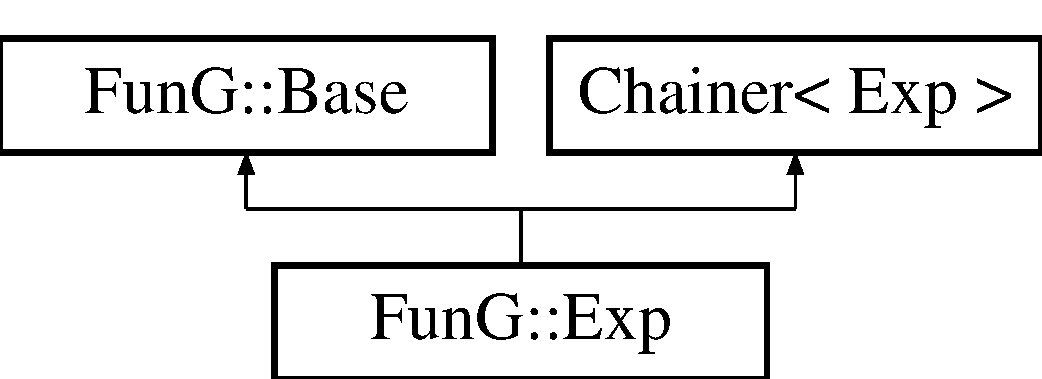
\includegraphics[height=2.000000cm]{structFunG_1_1Exp}
\end{center}
\end{figure}
\subsection*{Public Member Functions}
\begin{DoxyCompactItemize}
\item 
\hyperlink{structFunG_1_1Exp_a2abec31ebf5f8ee4877fb1c05d2fdad2}{Exp} (double x=0.)
\begin{DoxyCompactList}\small\item\em Function value. \end{DoxyCompactList}\item 
void \hyperlink{structFunG_1_1Exp_aabd4ab4e94bdc06bc1e773ffd023e0a7}{update} (double x)
\begin{DoxyCompactList}\small\item\em Set point of evaluation. \end{DoxyCompactList}\item 
double \hyperlink{structFunG_1_1Exp_a753d56db833507c33fe91714d119c755}{d0} () const noexcept
\begin{DoxyCompactList}\small\item\em Function value. \end{DoxyCompactList}\item 
double \hyperlink{structFunG_1_1Exp_ac02fb3f10f654a60fef470b271e26b41}{d1} (double dx=1.) const 
\begin{DoxyCompactList}\small\item\em Function value. \end{DoxyCompactList}\item 
double \hyperlink{structFunG_1_1Exp_a1a5b4e6b0cedb08548d0e83457908182}{d2} (double dx=1., double dy=1.) const 
\begin{DoxyCompactList}\small\item\em Function value. \end{DoxyCompactList}\item 
double \hyperlink{structFunG_1_1Exp_adea30657eb96144009f7cc96451391e8}{d3} (double dx=1., double dy=1., double dz=1.) const 
\begin{DoxyCompactList}\small\item\em Function value. \end{DoxyCompactList}\end{DoxyCompactItemize}


\subsection{Detailed Description}
Exponential function including first three derivatives. 

For scalar functions directional derivatives are less interesting. Incorporating this function as building block for more complex functions requires directional derivatives. These occur during applications of the chain rule. 

\subsection{Constructor \& Destructor Documentation}
\hypertarget{structFunG_1_1Exp_a2abec31ebf5f8ee4877fb1c05d2fdad2}{\index{Fun\-G\-::\-Exp@{Fun\-G\-::\-Exp}!Exp@{Exp}}
\index{Exp@{Exp}!FunG::Exp@{Fun\-G\-::\-Exp}}
\subsubsection[{Exp}]{\setlength{\rightskip}{0pt plus 5cm}Fun\-G\-::\-Exp\-::\-Exp (
\begin{DoxyParamCaption}
\item[{double}]{x = {\ttfamily 0.}}
\end{DoxyParamCaption}
)\hspace{0.3cm}{\ttfamily [inline]}, {\ttfamily [explicit]}}}\label{structFunG_1_1Exp_a2abec31ebf5f8ee4877fb1c05d2fdad2}


Function value. 



\subsection{Member Function Documentation}
\hypertarget{structFunG_1_1Exp_a753d56db833507c33fe91714d119c755}{\index{Fun\-G\-::\-Exp@{Fun\-G\-::\-Exp}!d0@{d0}}
\index{d0@{d0}!FunG::Exp@{Fun\-G\-::\-Exp}}
\subsubsection[{d0}]{\setlength{\rightskip}{0pt plus 5cm}double Fun\-G\-::\-Exp\-::d0 (
\begin{DoxyParamCaption}
{}
\end{DoxyParamCaption}
) const\hspace{0.3cm}{\ttfamily [inline]}, {\ttfamily [noexcept]}}}\label{structFunG_1_1Exp_a753d56db833507c33fe91714d119c755}


Function value. 

\hypertarget{structFunG_1_1Exp_ac02fb3f10f654a60fef470b271e26b41}{\index{Fun\-G\-::\-Exp@{Fun\-G\-::\-Exp}!d1@{d1}}
\index{d1@{d1}!FunG::Exp@{Fun\-G\-::\-Exp}}
\subsubsection[{d1}]{\setlength{\rightskip}{0pt plus 5cm}double Fun\-G\-::\-Exp\-::d1 (
\begin{DoxyParamCaption}
\item[{double}]{dx = {\ttfamily 1.}}
\end{DoxyParamCaption}
) const\hspace{0.3cm}{\ttfamily [inline]}}}\label{structFunG_1_1Exp_ac02fb3f10f654a60fef470b271e26b41}


Function value. 

\hypertarget{structFunG_1_1Exp_a1a5b4e6b0cedb08548d0e83457908182}{\index{Fun\-G\-::\-Exp@{Fun\-G\-::\-Exp}!d2@{d2}}
\index{d2@{d2}!FunG::Exp@{Fun\-G\-::\-Exp}}
\subsubsection[{d2}]{\setlength{\rightskip}{0pt plus 5cm}double Fun\-G\-::\-Exp\-::d2 (
\begin{DoxyParamCaption}
\item[{double}]{dx = {\ttfamily 1.}, }
\item[{double}]{dy = {\ttfamily 1.}}
\end{DoxyParamCaption}
) const\hspace{0.3cm}{\ttfamily [inline]}}}\label{structFunG_1_1Exp_a1a5b4e6b0cedb08548d0e83457908182}


Function value. 

\hypertarget{structFunG_1_1Exp_adea30657eb96144009f7cc96451391e8}{\index{Fun\-G\-::\-Exp@{Fun\-G\-::\-Exp}!d3@{d3}}
\index{d3@{d3}!FunG::Exp@{Fun\-G\-::\-Exp}}
\subsubsection[{d3}]{\setlength{\rightskip}{0pt plus 5cm}double Fun\-G\-::\-Exp\-::d3 (
\begin{DoxyParamCaption}
\item[{double}]{dx = {\ttfamily 1.}, }
\item[{double}]{dy = {\ttfamily 1.}, }
\item[{double}]{dz = {\ttfamily 1.}}
\end{DoxyParamCaption}
) const\hspace{0.3cm}{\ttfamily [inline]}}}\label{structFunG_1_1Exp_adea30657eb96144009f7cc96451391e8}


Function value. 

\hypertarget{structFunG_1_1Exp_aabd4ab4e94bdc06bc1e773ffd023e0a7}{\index{Fun\-G\-::\-Exp@{Fun\-G\-::\-Exp}!update@{update}}
\index{update@{update}!FunG::Exp@{Fun\-G\-::\-Exp}}
\subsubsection[{update}]{\setlength{\rightskip}{0pt plus 5cm}void Fun\-G\-::\-Exp\-::update (
\begin{DoxyParamCaption}
\item[{double}]{x}
\end{DoxyParamCaption}
)\hspace{0.3cm}{\ttfamily [inline]}}}\label{structFunG_1_1Exp_aabd4ab4e94bdc06bc1e773ffd023e0a7}


Set point of evaluation. 



The documentation for this struct was generated from the following file\-:\begin{DoxyCompactItemize}
\item 
include/fung/cmath/\hyperlink{cmath_2exp_8hh}{exp.\-hh}\end{DoxyCompactItemize}

\hypertarget{structFunG_1_1texify_1_1Exp}{\section{Fun\-G\-:\-:texify\-:\-:Exp Struct Reference}
\label{structFunG_1_1texify_1_1Exp}\index{Fun\-G\-::texify\-::\-Exp@{Fun\-G\-::texify\-::\-Exp}}
}


{\ttfamily \#include $<$exp.\-hh$>$}

Inheritance diagram for Fun\-G\-:\-:texify\-:\-:Exp\-:\begin{figure}[H]
\begin{center}
\leavevmode
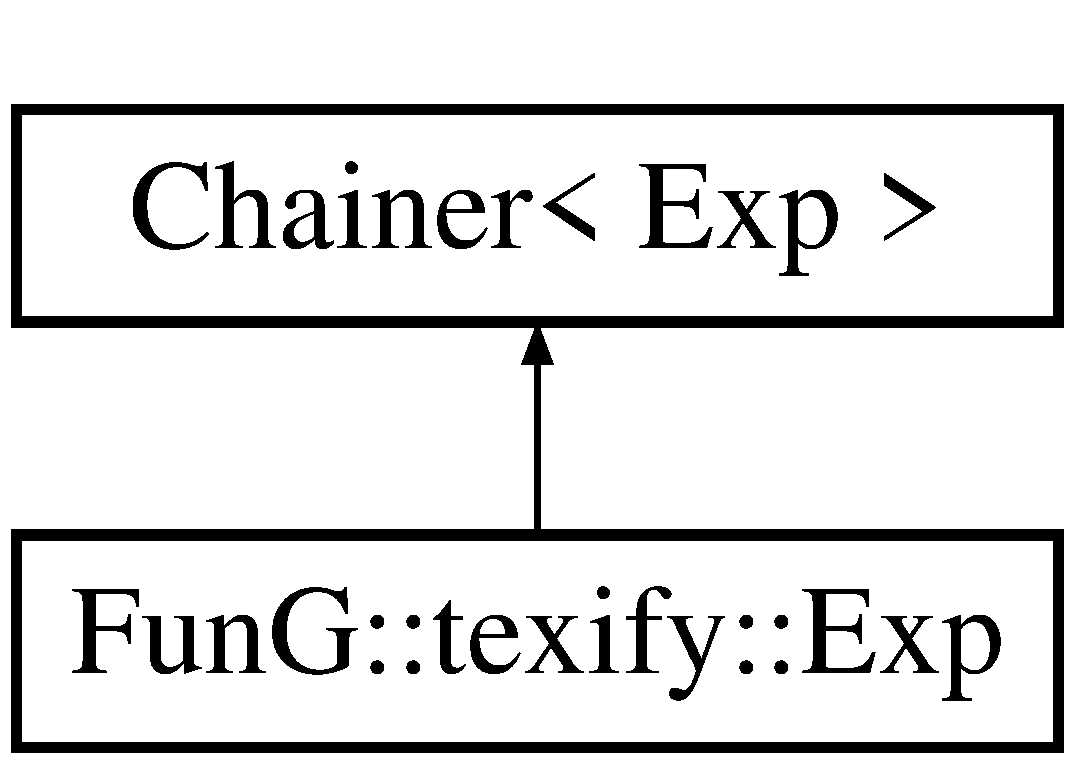
\includegraphics[height=2.000000cm]{structFunG_1_1texify_1_1Exp}
\end{center}
\end{figure}
\subsection*{Public Member Functions}
\begin{DoxyCompactItemize}
\item 
\hyperlink{structFunG_1_1texify_1_1Exp_a781def06b8991754ab8ede94835a0bb7}{Exp} (const std\-::string \&x=\char`\"{}x\char`\"{})
\begin{DoxyCompactList}\small\item\em Function value. \end{DoxyCompactList}\item 
void \hyperlink{structFunG_1_1texify_1_1Exp_ab4fccc070c983d0aebb5b4bc46930bfd}{update} (const std\-::string \&x)
\begin{DoxyCompactList}\small\item\em Set point of evaluation. \end{DoxyCompactList}\item 
std\-::string \hyperlink{structFunG_1_1texify_1_1Exp_a88d18f5948309158226a6a85e02c3009}{d0} () const noexcept
\begin{DoxyCompactList}\small\item\em Function value. \end{DoxyCompactList}\item 
std\-::string \hyperlink{structFunG_1_1texify_1_1Exp_a72d4392ee43c7e5ab78b9142fcd8713c}{d1} (const std\-::string \&dx=\char`\"{}\char`\"{}) const 
\begin{DoxyCompactList}\small\item\em Function value. \end{DoxyCompactList}\item 
std\-::string \hyperlink{structFunG_1_1texify_1_1Exp_a8213415ca7f51ebf0515e287a2feafb2}{d2} (const std\-::string \&dx=\char`\"{}\char`\"{}, const std\-::string \&dy=\char`\"{}\char`\"{}) const 
\begin{DoxyCompactList}\small\item\em Function value. \end{DoxyCompactList}\item 
std\-::string \hyperlink{structFunG_1_1texify_1_1Exp_a3e6d06ab346d0d076069cbfdba90b501}{d3} (const std\-::string \&dx=\char`\"{}\char`\"{}, const std\-::string \&dy=\char`\"{}\char`\"{}, const std\-::string \&dz=\char`\"{}\char`\"{}) const 
\begin{DoxyCompactList}\small\item\em Function value. \end{DoxyCompactList}\end{DoxyCompactItemize}


\subsection{Constructor \& Destructor Documentation}
\hypertarget{structFunG_1_1texify_1_1Exp_a781def06b8991754ab8ede94835a0bb7}{\index{Fun\-G\-::texify\-::\-Exp@{Fun\-G\-::texify\-::\-Exp}!Exp@{Exp}}
\index{Exp@{Exp}!FunG::texify::Exp@{Fun\-G\-::texify\-::\-Exp}}
\subsubsection[{Exp}]{\setlength{\rightskip}{0pt plus 5cm}Fun\-G\-::texify\-::\-Exp\-::\-Exp (
\begin{DoxyParamCaption}
\item[{const std\-::string \&}]{x = {\ttfamily \char`\"{}x\char`\"{}}}
\end{DoxyParamCaption}
)\hspace{0.3cm}{\ttfamily [inline]}, {\ttfamily [explicit]}}}\label{structFunG_1_1texify_1_1Exp_a781def06b8991754ab8ede94835a0bb7}


Function value. 



\subsection{Member Function Documentation}
\hypertarget{structFunG_1_1texify_1_1Exp_a88d18f5948309158226a6a85e02c3009}{\index{Fun\-G\-::texify\-::\-Exp@{Fun\-G\-::texify\-::\-Exp}!d0@{d0}}
\index{d0@{d0}!FunG::texify::Exp@{Fun\-G\-::texify\-::\-Exp}}
\subsubsection[{d0}]{\setlength{\rightskip}{0pt plus 5cm}std\-::string Fun\-G\-::texify\-::\-Exp\-::d0 (
\begin{DoxyParamCaption}
{}
\end{DoxyParamCaption}
) const\hspace{0.3cm}{\ttfamily [inline]}, {\ttfamily [noexcept]}}}\label{structFunG_1_1texify_1_1Exp_a88d18f5948309158226a6a85e02c3009}


Function value. 

\hypertarget{structFunG_1_1texify_1_1Exp_a72d4392ee43c7e5ab78b9142fcd8713c}{\index{Fun\-G\-::texify\-::\-Exp@{Fun\-G\-::texify\-::\-Exp}!d1@{d1}}
\index{d1@{d1}!FunG::texify::Exp@{Fun\-G\-::texify\-::\-Exp}}
\subsubsection[{d1}]{\setlength{\rightskip}{0pt plus 5cm}std\-::string Fun\-G\-::texify\-::\-Exp\-::d1 (
\begin{DoxyParamCaption}
\item[{const std\-::string \&}]{dx = {\ttfamily \char`\"{}\char`\"{}}}
\end{DoxyParamCaption}
) const\hspace{0.3cm}{\ttfamily [inline]}}}\label{structFunG_1_1texify_1_1Exp_a72d4392ee43c7e5ab78b9142fcd8713c}


Function value. 

\hypertarget{structFunG_1_1texify_1_1Exp_a8213415ca7f51ebf0515e287a2feafb2}{\index{Fun\-G\-::texify\-::\-Exp@{Fun\-G\-::texify\-::\-Exp}!d2@{d2}}
\index{d2@{d2}!FunG::texify::Exp@{Fun\-G\-::texify\-::\-Exp}}
\subsubsection[{d2}]{\setlength{\rightskip}{0pt plus 5cm}std\-::string Fun\-G\-::texify\-::\-Exp\-::d2 (
\begin{DoxyParamCaption}
\item[{const std\-::string \&}]{dx = {\ttfamily \char`\"{}\char`\"{}}, }
\item[{const std\-::string \&}]{dy = {\ttfamily \char`\"{}\char`\"{}}}
\end{DoxyParamCaption}
) const\hspace{0.3cm}{\ttfamily [inline]}}}\label{structFunG_1_1texify_1_1Exp_a8213415ca7f51ebf0515e287a2feafb2}


Function value. 

\hypertarget{structFunG_1_1texify_1_1Exp_a3e6d06ab346d0d076069cbfdba90b501}{\index{Fun\-G\-::texify\-::\-Exp@{Fun\-G\-::texify\-::\-Exp}!d3@{d3}}
\index{d3@{d3}!FunG::texify::Exp@{Fun\-G\-::texify\-::\-Exp}}
\subsubsection[{d3}]{\setlength{\rightskip}{0pt plus 5cm}std\-::string Fun\-G\-::texify\-::\-Exp\-::d3 (
\begin{DoxyParamCaption}
\item[{const std\-::string \&}]{dx = {\ttfamily \char`\"{}\char`\"{}}, }
\item[{const std\-::string \&}]{dy = {\ttfamily \char`\"{}\char`\"{}}, }
\item[{const std\-::string \&}]{dz = {\ttfamily \char`\"{}\char`\"{}}}
\end{DoxyParamCaption}
) const\hspace{0.3cm}{\ttfamily [inline]}}}\label{structFunG_1_1texify_1_1Exp_a3e6d06ab346d0d076069cbfdba90b501}


Function value. 

\hypertarget{structFunG_1_1texify_1_1Exp_ab4fccc070c983d0aebb5b4bc46930bfd}{\index{Fun\-G\-::texify\-::\-Exp@{Fun\-G\-::texify\-::\-Exp}!update@{update}}
\index{update@{update}!FunG::texify::Exp@{Fun\-G\-::texify\-::\-Exp}}
\subsubsection[{update}]{\setlength{\rightskip}{0pt plus 5cm}void Fun\-G\-::texify\-::\-Exp\-::update (
\begin{DoxyParamCaption}
\item[{const std\-::string \&}]{x}
\end{DoxyParamCaption}
)\hspace{0.3cm}{\ttfamily [inline]}}}\label{structFunG_1_1texify_1_1Exp_ab4fccc070c983d0aebb5b4bc46930bfd}


Set point of evaluation. 



The documentation for this struct was generated from the following file\-:\begin{DoxyCompactItemize}
\item 
include/fung/texify/cmath/\hyperlink{texify_2cmath_2exp_8hh}{exp.\-hh}\end{DoxyCompactItemize}

\hypertarget{structFunG_1_1stringify_1_1Exp}{\section{Fun\-G\-:\-:stringify\-:\-:Exp Struct Reference}
\label{structFunG_1_1stringify_1_1Exp}\index{Fun\-G\-::stringify\-::\-Exp@{Fun\-G\-::stringify\-::\-Exp}}
}


{\ttfamily \#include $<$exp.\-hh$>$}

Inheritance diagram for Fun\-G\-:\-:stringify\-:\-:Exp\-:\begin{figure}[H]
\begin{center}
\leavevmode
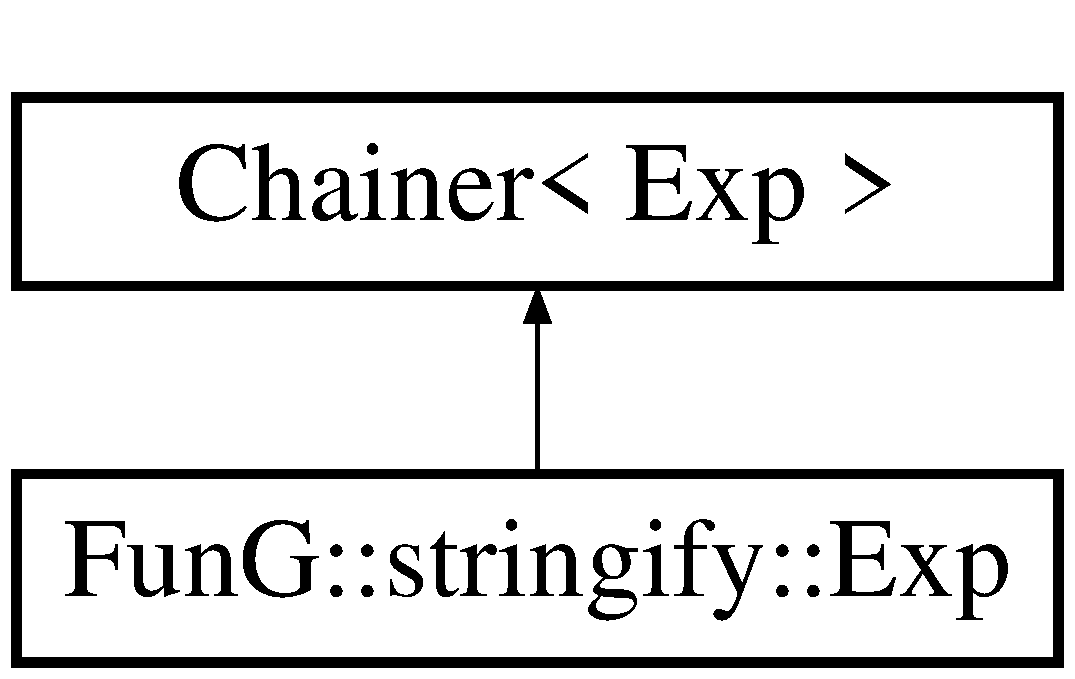
\includegraphics[height=2.000000cm]{structFunG_1_1stringify_1_1Exp}
\end{center}
\end{figure}
\subsection*{Public Member Functions}
\begin{DoxyCompactItemize}
\item 
\hyperlink{structFunG_1_1stringify_1_1Exp_a70a0b1639fa4ea5ffbf37345d3d8de53}{Exp} (const std\-::string \&x=\char`\"{}x\char`\"{})
\begin{DoxyCompactList}\small\item\em Function value. \end{DoxyCompactList}\item 
void \hyperlink{structFunG_1_1stringify_1_1Exp_a5a2e79edbfa8073ad68e27b9cb27468f}{update} (const std\-::string \&x)
\begin{DoxyCompactList}\small\item\em Set point of evaluation. \end{DoxyCompactList}\item 
std\-::string \hyperlink{structFunG_1_1stringify_1_1Exp_a1ad860a95100cc31f7cdf5e1f37f60cd}{d0} () const noexcept
\begin{DoxyCompactList}\small\item\em Function value. \end{DoxyCompactList}\item 
std\-::string \hyperlink{structFunG_1_1stringify_1_1Exp_a3e6070ac1dbb3ce42795c6d84a29d21a}{d1} (const std\-::string \&dx=\char`\"{}\char`\"{}) const 
\begin{DoxyCompactList}\small\item\em Function value. \end{DoxyCompactList}\item 
std\-::string \hyperlink{structFunG_1_1stringify_1_1Exp_a25a7af7e815699e09d277d6640f6b6f3}{d2} (const std\-::string \&dx=\char`\"{}\char`\"{}, const std\-::string \&dy=\char`\"{}\char`\"{}) const 
\begin{DoxyCompactList}\small\item\em Function value. \end{DoxyCompactList}\item 
std\-::string \hyperlink{structFunG_1_1stringify_1_1Exp_a8fbdc564252405abfa2c13f52e6b3e91}{d3} (const std\-::string \&dx=\char`\"{}\char`\"{}, const std\-::string \&dy=\char`\"{}\char`\"{}, const std\-::string \&dz=\char`\"{}\char`\"{}) const 
\begin{DoxyCompactList}\small\item\em Function value. \end{DoxyCompactList}\end{DoxyCompactItemize}


\subsection{Constructor \& Destructor Documentation}
\hypertarget{structFunG_1_1stringify_1_1Exp_a70a0b1639fa4ea5ffbf37345d3d8de53}{\index{Fun\-G\-::stringify\-::\-Exp@{Fun\-G\-::stringify\-::\-Exp}!Exp@{Exp}}
\index{Exp@{Exp}!FunG::stringify::Exp@{Fun\-G\-::stringify\-::\-Exp}}
\subsubsection[{Exp}]{\setlength{\rightskip}{0pt plus 5cm}Fun\-G\-::stringify\-::\-Exp\-::\-Exp (
\begin{DoxyParamCaption}
\item[{const std\-::string \&}]{x = {\ttfamily \char`\"{}x\char`\"{}}}
\end{DoxyParamCaption}
)\hspace{0.3cm}{\ttfamily [inline]}, {\ttfamily [explicit]}}}\label{structFunG_1_1stringify_1_1Exp_a70a0b1639fa4ea5ffbf37345d3d8de53}


Function value. 



\subsection{Member Function Documentation}
\hypertarget{structFunG_1_1stringify_1_1Exp_a1ad860a95100cc31f7cdf5e1f37f60cd}{\index{Fun\-G\-::stringify\-::\-Exp@{Fun\-G\-::stringify\-::\-Exp}!d0@{d0}}
\index{d0@{d0}!FunG::stringify::Exp@{Fun\-G\-::stringify\-::\-Exp}}
\subsubsection[{d0}]{\setlength{\rightskip}{0pt plus 5cm}std\-::string Fun\-G\-::stringify\-::\-Exp\-::d0 (
\begin{DoxyParamCaption}
{}
\end{DoxyParamCaption}
) const\hspace{0.3cm}{\ttfamily [inline]}, {\ttfamily [noexcept]}}}\label{structFunG_1_1stringify_1_1Exp_a1ad860a95100cc31f7cdf5e1f37f60cd}


Function value. 

\hypertarget{structFunG_1_1stringify_1_1Exp_a3e6070ac1dbb3ce42795c6d84a29d21a}{\index{Fun\-G\-::stringify\-::\-Exp@{Fun\-G\-::stringify\-::\-Exp}!d1@{d1}}
\index{d1@{d1}!FunG::stringify::Exp@{Fun\-G\-::stringify\-::\-Exp}}
\subsubsection[{d1}]{\setlength{\rightskip}{0pt plus 5cm}std\-::string Fun\-G\-::stringify\-::\-Exp\-::d1 (
\begin{DoxyParamCaption}
\item[{const std\-::string \&}]{dx = {\ttfamily \char`\"{}\char`\"{}}}
\end{DoxyParamCaption}
) const\hspace{0.3cm}{\ttfamily [inline]}}}\label{structFunG_1_1stringify_1_1Exp_a3e6070ac1dbb3ce42795c6d84a29d21a}


Function value. 

\hypertarget{structFunG_1_1stringify_1_1Exp_a25a7af7e815699e09d277d6640f6b6f3}{\index{Fun\-G\-::stringify\-::\-Exp@{Fun\-G\-::stringify\-::\-Exp}!d2@{d2}}
\index{d2@{d2}!FunG::stringify::Exp@{Fun\-G\-::stringify\-::\-Exp}}
\subsubsection[{d2}]{\setlength{\rightskip}{0pt plus 5cm}std\-::string Fun\-G\-::stringify\-::\-Exp\-::d2 (
\begin{DoxyParamCaption}
\item[{const std\-::string \&}]{dx = {\ttfamily \char`\"{}\char`\"{}}, }
\item[{const std\-::string \&}]{dy = {\ttfamily \char`\"{}\char`\"{}}}
\end{DoxyParamCaption}
) const\hspace{0.3cm}{\ttfamily [inline]}}}\label{structFunG_1_1stringify_1_1Exp_a25a7af7e815699e09d277d6640f6b6f3}


Function value. 

\hypertarget{structFunG_1_1stringify_1_1Exp_a8fbdc564252405abfa2c13f52e6b3e91}{\index{Fun\-G\-::stringify\-::\-Exp@{Fun\-G\-::stringify\-::\-Exp}!d3@{d3}}
\index{d3@{d3}!FunG::stringify::Exp@{Fun\-G\-::stringify\-::\-Exp}}
\subsubsection[{d3}]{\setlength{\rightskip}{0pt plus 5cm}std\-::string Fun\-G\-::stringify\-::\-Exp\-::d3 (
\begin{DoxyParamCaption}
\item[{const std\-::string \&}]{dx = {\ttfamily \char`\"{}\char`\"{}}, }
\item[{const std\-::string \&}]{dy = {\ttfamily \char`\"{}\char`\"{}}, }
\item[{const std\-::string \&}]{dz = {\ttfamily \char`\"{}\char`\"{}}}
\end{DoxyParamCaption}
) const\hspace{0.3cm}{\ttfamily [inline]}}}\label{structFunG_1_1stringify_1_1Exp_a8fbdc564252405abfa2c13f52e6b3e91}


Function value. 

\hypertarget{structFunG_1_1stringify_1_1Exp_a5a2e79edbfa8073ad68e27b9cb27468f}{\index{Fun\-G\-::stringify\-::\-Exp@{Fun\-G\-::stringify\-::\-Exp}!update@{update}}
\index{update@{update}!FunG::stringify::Exp@{Fun\-G\-::stringify\-::\-Exp}}
\subsubsection[{update}]{\setlength{\rightskip}{0pt plus 5cm}void Fun\-G\-::stringify\-::\-Exp\-::update (
\begin{DoxyParamCaption}
\item[{const std\-::string \&}]{x}
\end{DoxyParamCaption}
)\hspace{0.3cm}{\ttfamily [inline]}}}\label{structFunG_1_1stringify_1_1Exp_a5a2e79edbfa8073ad68e27b9cb27468f}


Set point of evaluation. 



The documentation for this struct was generated from the following file\-:\begin{DoxyCompactItemize}
\item 
include/fung/cmath/stringify/\hyperlink{stringify_2exp_8hh}{exp.\-hh}\end{DoxyCompactItemize}

\hypertarget{structFunG_1_1Exp2}{\section{Fun\-G\-:\-:Exp2 Struct Reference}
\label{structFunG_1_1Exp2}\index{Fun\-G\-::\-Exp2@{Fun\-G\-::\-Exp2}}
}


Function $2^x$ including first three derivatives.  




{\ttfamily \#include $<$exp.\-hh$>$}

Inheritance diagram for Fun\-G\-:\-:Exp2\-:\begin{figure}[H]
\begin{center}
\leavevmode
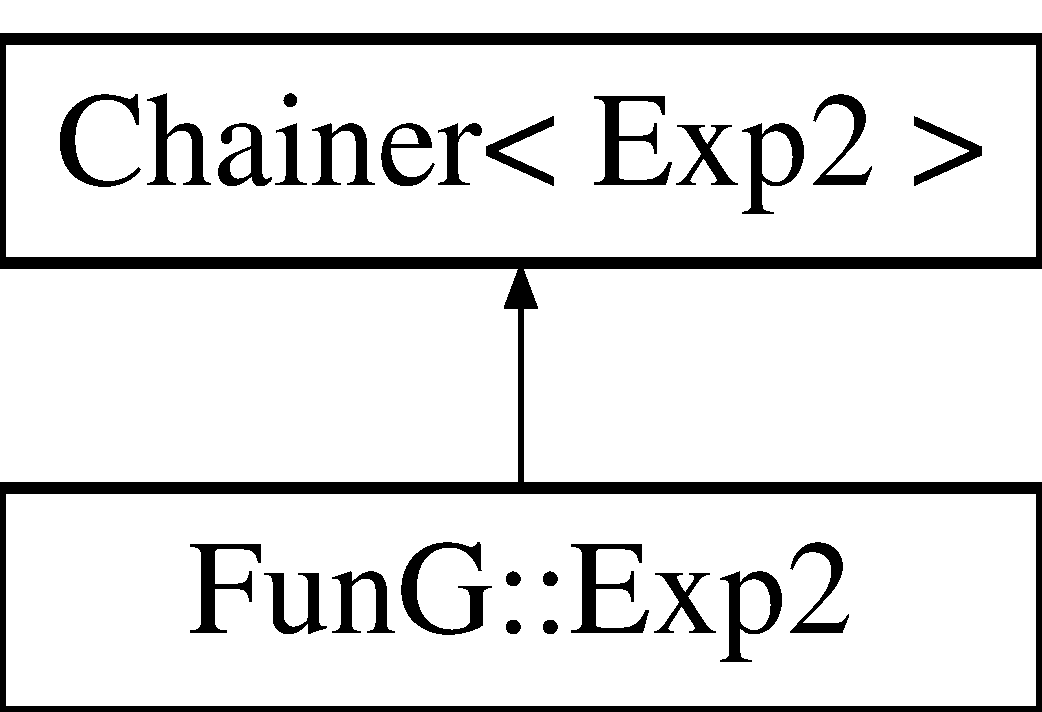
\includegraphics[height=2.000000cm]{structFunG_1_1Exp2}
\end{center}
\end{figure}
\subsection*{Public Member Functions}
\begin{DoxyCompactItemize}
\item 
\hyperlink{structFunG_1_1Exp2_aa5e03d1e3a39a1c2151cdfe092461060}{Exp2} (double x=0.)
\begin{DoxyCompactList}\small\item\em Constructor. \end{DoxyCompactList}\item 
void \hyperlink{structFunG_1_1Exp2_a256e50dac0e06814d2fb150ac997ea5d}{update} (double x)
\begin{DoxyCompactList}\small\item\em Set point of evaluation. \end{DoxyCompactList}\item 
double \hyperlink{structFunG_1_1Exp2_a70a452fa4b190e2c427fd87f17c98dc5}{d0} () const noexcept
\begin{DoxyCompactList}\small\item\em Function value. \end{DoxyCompactList}\item 
double \hyperlink{structFunG_1_1Exp2_a45eae0e2d4a7d3ec8c02eeb237fcc8ae}{d1} (double dx=1.) const 
\begin{DoxyCompactList}\small\item\em First (directional) derivative. \end{DoxyCompactList}\item 
double \hyperlink{structFunG_1_1Exp2_a5f4e6755ebce5994f79a0711725bf9a3}{d2} (double dx=1., double dy=1.) const 
\begin{DoxyCompactList}\small\item\em Second (directional) derivative. \end{DoxyCompactList}\item 
double \hyperlink{structFunG_1_1Exp2_aff3797bff08d2ec89a72a8ce7779d08e}{d3} (double dx=1., double dy=1., double dz=1.) const 
\begin{DoxyCompactList}\small\item\em Third (directional) derivative. \end{DoxyCompactList}\end{DoxyCompactItemize}


\subsection{Detailed Description}
Function $2^x$ including first three derivatives. 

For scalar functions directional derivatives are less interesting. Incorporating this function as building block for more complex functions requires directional derivatives. These occur during applications of the chain rule. 

\subsection{Constructor \& Destructor Documentation}
\hypertarget{structFunG_1_1Exp2_aa5e03d1e3a39a1c2151cdfe092461060}{\index{Fun\-G\-::\-Exp2@{Fun\-G\-::\-Exp2}!Exp2@{Exp2}}
\index{Exp2@{Exp2}!FunG::Exp2@{Fun\-G\-::\-Exp2}}
\subsubsection[{Exp2}]{\setlength{\rightskip}{0pt plus 5cm}Fun\-G\-::\-Exp2\-::\-Exp2 (
\begin{DoxyParamCaption}
\item[{double}]{x = {\ttfamily 0.}}
\end{DoxyParamCaption}
)\hspace{0.3cm}{\ttfamily [inline]}, {\ttfamily [explicit]}}}\label{structFunG_1_1Exp2_aa5e03d1e3a39a1c2151cdfe092461060}


Constructor. 


\begin{DoxyParams}{Parameters}
{\em x} & point of evaluation \\
\hline
\end{DoxyParams}


\subsection{Member Function Documentation}
\hypertarget{structFunG_1_1Exp2_a70a452fa4b190e2c427fd87f17c98dc5}{\index{Fun\-G\-::\-Exp2@{Fun\-G\-::\-Exp2}!d0@{d0}}
\index{d0@{d0}!FunG::Exp2@{Fun\-G\-::\-Exp2}}
\subsubsection[{d0}]{\setlength{\rightskip}{0pt plus 5cm}double Fun\-G\-::\-Exp2\-::d0 (
\begin{DoxyParamCaption}
{}
\end{DoxyParamCaption}
) const\hspace{0.3cm}{\ttfamily [inline]}, {\ttfamily [noexcept]}}}\label{structFunG_1_1Exp2_a70a452fa4b190e2c427fd87f17c98dc5}


Function value. 

\hypertarget{structFunG_1_1Exp2_a45eae0e2d4a7d3ec8c02eeb237fcc8ae}{\index{Fun\-G\-::\-Exp2@{Fun\-G\-::\-Exp2}!d1@{d1}}
\index{d1@{d1}!FunG::Exp2@{Fun\-G\-::\-Exp2}}
\subsubsection[{d1}]{\setlength{\rightskip}{0pt plus 5cm}double Fun\-G\-::\-Exp2\-::d1 (
\begin{DoxyParamCaption}
\item[{double}]{dx = {\ttfamily 1.}}
\end{DoxyParamCaption}
) const\hspace{0.3cm}{\ttfamily [inline]}}}\label{structFunG_1_1Exp2_a45eae0e2d4a7d3ec8c02eeb237fcc8ae}


First (directional) derivative. 

\hypertarget{structFunG_1_1Exp2_a5f4e6755ebce5994f79a0711725bf9a3}{\index{Fun\-G\-::\-Exp2@{Fun\-G\-::\-Exp2}!d2@{d2}}
\index{d2@{d2}!FunG::Exp2@{Fun\-G\-::\-Exp2}}
\subsubsection[{d2}]{\setlength{\rightskip}{0pt plus 5cm}double Fun\-G\-::\-Exp2\-::d2 (
\begin{DoxyParamCaption}
\item[{double}]{dx = {\ttfamily 1.}, }
\item[{double}]{dy = {\ttfamily 1.}}
\end{DoxyParamCaption}
) const\hspace{0.3cm}{\ttfamily [inline]}}}\label{structFunG_1_1Exp2_a5f4e6755ebce5994f79a0711725bf9a3}


Second (directional) derivative. 

\hypertarget{structFunG_1_1Exp2_aff3797bff08d2ec89a72a8ce7779d08e}{\index{Fun\-G\-::\-Exp2@{Fun\-G\-::\-Exp2}!d3@{d3}}
\index{d3@{d3}!FunG::Exp2@{Fun\-G\-::\-Exp2}}
\subsubsection[{d3}]{\setlength{\rightskip}{0pt plus 5cm}double Fun\-G\-::\-Exp2\-::d3 (
\begin{DoxyParamCaption}
\item[{double}]{dx = {\ttfamily 1.}, }
\item[{double}]{dy = {\ttfamily 1.}, }
\item[{double}]{dz = {\ttfamily 1.}}
\end{DoxyParamCaption}
) const\hspace{0.3cm}{\ttfamily [inline]}}}\label{structFunG_1_1Exp2_aff3797bff08d2ec89a72a8ce7779d08e}


Third (directional) derivative. 

\hypertarget{structFunG_1_1Exp2_a256e50dac0e06814d2fb150ac997ea5d}{\index{Fun\-G\-::\-Exp2@{Fun\-G\-::\-Exp2}!update@{update}}
\index{update@{update}!FunG::Exp2@{Fun\-G\-::\-Exp2}}
\subsubsection[{update}]{\setlength{\rightskip}{0pt plus 5cm}void Fun\-G\-::\-Exp2\-::update (
\begin{DoxyParamCaption}
\item[{double}]{x}
\end{DoxyParamCaption}
)\hspace{0.3cm}{\ttfamily [inline]}}}\label{structFunG_1_1Exp2_a256e50dac0e06814d2fb150ac997ea5d}


Set point of evaluation. 



The documentation for this struct was generated from the following file\-:\begin{DoxyCompactItemize}
\item 
include/fung/cmath/\hyperlink{exp_8hh}{exp.\-hh}\end{DoxyCompactItemize}

\hypertarget{structFunG_1_1texify_1_1Exp2}{\section{Fun\-G\-:\-:texify\-:\-:Exp2 Struct Reference}
\label{structFunG_1_1texify_1_1Exp2}\index{Fun\-G\-::texify\-::\-Exp2@{Fun\-G\-::texify\-::\-Exp2}}
}


Function $2^x$ including first three derivatives.  




{\ttfamily \#include $<$exp.\-hh$>$}

Inheritance diagram for Fun\-G\-:\-:texify\-:\-:Exp2\-:\begin{figure}[H]
\begin{center}
\leavevmode
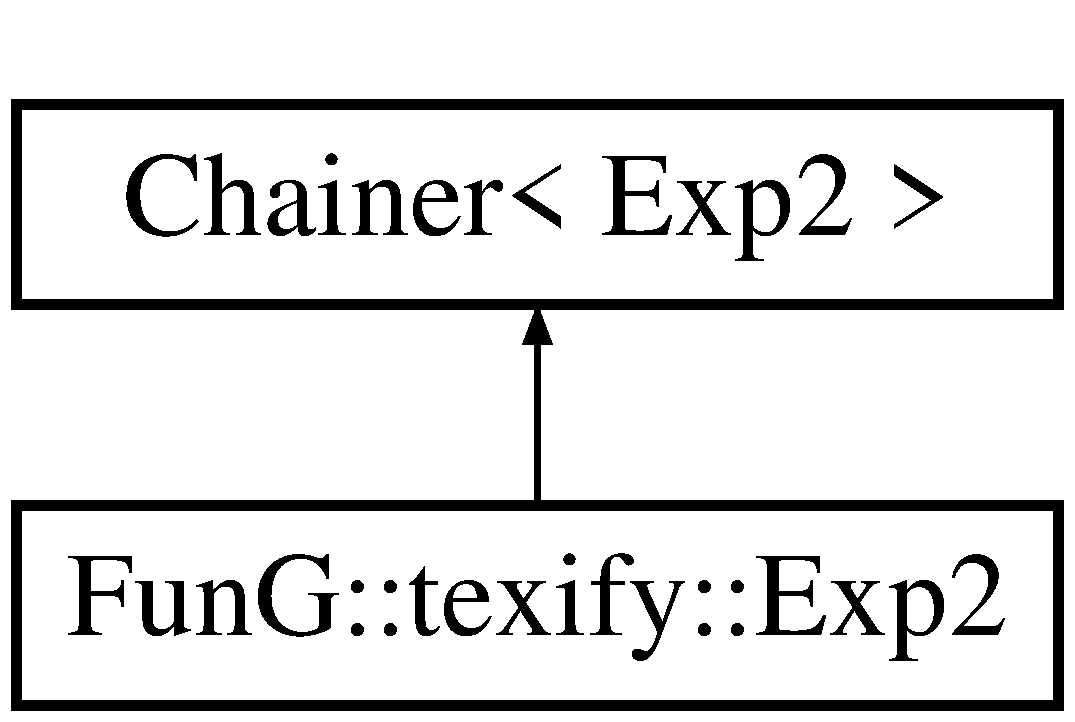
\includegraphics[height=2.000000cm]{structFunG_1_1texify_1_1Exp2}
\end{center}
\end{figure}
\subsection*{Public Member Functions}
\begin{DoxyCompactItemize}
\item 
\hyperlink{structFunG_1_1texify_1_1Exp2_a6b57152cf70e74701f720965c613bbae}{Exp2} (const std\-::string \&x=\char`\"{}x\char`\"{})
\begin{DoxyCompactList}\small\item\em Constructor. \end{DoxyCompactList}\item 
void \hyperlink{structFunG_1_1texify_1_1Exp2_a6974ebc03352e60aa1051e68ace44c4e}{update} (const std\-::string \&x)
\begin{DoxyCompactList}\small\item\em Set point of evaluation. \end{DoxyCompactList}\item 
std\-::string \hyperlink{structFunG_1_1texify_1_1Exp2_a7a59e0578272b13a9eca5c570e988946}{d0} () const noexcept
\begin{DoxyCompactList}\small\item\em Function value. \end{DoxyCompactList}\item 
std\-::string \hyperlink{structFunG_1_1texify_1_1Exp2_a842212da4f9684aff19b1f02777d27e4}{d1} (const std\-::string \&dx=\char`\"{}\char`\"{}) const 
\begin{DoxyCompactList}\small\item\em First (directional) derivative. \end{DoxyCompactList}\item 
std\-::string \hyperlink{structFunG_1_1texify_1_1Exp2_a2da97ece074e43301dd9c49568782fa2}{d2} (const std\-::string \&dx=\char`\"{}\char`\"{}, const std\-::string \&dy=\char`\"{}\char`\"{}) const 
\begin{DoxyCompactList}\small\item\em Second (directional) derivative. \end{DoxyCompactList}\item 
std\-::string \hyperlink{structFunG_1_1texify_1_1Exp2_acef5ff4d530388c59bd76ab1c6329776}{d3} (const std\-::string \&dx=\char`\"{}\char`\"{}, const std\-::string \&dy=\char`\"{}\char`\"{}, const std\-::string \&dz=\char`\"{}\char`\"{}) const 
\begin{DoxyCompactList}\small\item\em Third (directional) derivative. \end{DoxyCompactList}\end{DoxyCompactItemize}


\subsection{Detailed Description}
Function $2^x$ including first three derivatives. 

For scalar functions directional derivatives are less interesting. Incorporating this function as building block for more complex functions requires directional derivatives. These occur during applications of the chain rule. 

\subsection{Constructor \& Destructor Documentation}
\hypertarget{structFunG_1_1texify_1_1Exp2_a6b57152cf70e74701f720965c613bbae}{\index{Fun\-G\-::texify\-::\-Exp2@{Fun\-G\-::texify\-::\-Exp2}!Exp2@{Exp2}}
\index{Exp2@{Exp2}!FunG::texify::Exp2@{Fun\-G\-::texify\-::\-Exp2}}
\subsubsection[{Exp2}]{\setlength{\rightskip}{0pt plus 5cm}Fun\-G\-::texify\-::\-Exp2\-::\-Exp2 (
\begin{DoxyParamCaption}
\item[{const std\-::string \&}]{x = {\ttfamily \char`\"{}x\char`\"{}}}
\end{DoxyParamCaption}
)\hspace{0.3cm}{\ttfamily [inline]}, {\ttfamily [explicit]}}}\label{structFunG_1_1texify_1_1Exp2_a6b57152cf70e74701f720965c613bbae}


Constructor. 


\begin{DoxyParams}{Parameters}
{\em x} & point of evaluation \\
\hline
\end{DoxyParams}


\subsection{Member Function Documentation}
\hypertarget{structFunG_1_1texify_1_1Exp2_a7a59e0578272b13a9eca5c570e988946}{\index{Fun\-G\-::texify\-::\-Exp2@{Fun\-G\-::texify\-::\-Exp2}!d0@{d0}}
\index{d0@{d0}!FunG::texify::Exp2@{Fun\-G\-::texify\-::\-Exp2}}
\subsubsection[{d0}]{\setlength{\rightskip}{0pt plus 5cm}std\-::string Fun\-G\-::texify\-::\-Exp2\-::d0 (
\begin{DoxyParamCaption}
{}
\end{DoxyParamCaption}
) const\hspace{0.3cm}{\ttfamily [inline]}, {\ttfamily [noexcept]}}}\label{structFunG_1_1texify_1_1Exp2_a7a59e0578272b13a9eca5c570e988946}


Function value. 

\hypertarget{structFunG_1_1texify_1_1Exp2_a842212da4f9684aff19b1f02777d27e4}{\index{Fun\-G\-::texify\-::\-Exp2@{Fun\-G\-::texify\-::\-Exp2}!d1@{d1}}
\index{d1@{d1}!FunG::texify::Exp2@{Fun\-G\-::texify\-::\-Exp2}}
\subsubsection[{d1}]{\setlength{\rightskip}{0pt plus 5cm}std\-::string Fun\-G\-::texify\-::\-Exp2\-::d1 (
\begin{DoxyParamCaption}
\item[{const std\-::string \&}]{dx = {\ttfamily \char`\"{}\char`\"{}}}
\end{DoxyParamCaption}
) const\hspace{0.3cm}{\ttfamily [inline]}}}\label{structFunG_1_1texify_1_1Exp2_a842212da4f9684aff19b1f02777d27e4}


First (directional) derivative. 

\hypertarget{structFunG_1_1texify_1_1Exp2_a2da97ece074e43301dd9c49568782fa2}{\index{Fun\-G\-::texify\-::\-Exp2@{Fun\-G\-::texify\-::\-Exp2}!d2@{d2}}
\index{d2@{d2}!FunG::texify::Exp2@{Fun\-G\-::texify\-::\-Exp2}}
\subsubsection[{d2}]{\setlength{\rightskip}{0pt plus 5cm}std\-::string Fun\-G\-::texify\-::\-Exp2\-::d2 (
\begin{DoxyParamCaption}
\item[{const std\-::string \&}]{dx = {\ttfamily \char`\"{}\char`\"{}}, }
\item[{const std\-::string \&}]{dy = {\ttfamily \char`\"{}\char`\"{}}}
\end{DoxyParamCaption}
) const\hspace{0.3cm}{\ttfamily [inline]}}}\label{structFunG_1_1texify_1_1Exp2_a2da97ece074e43301dd9c49568782fa2}


Second (directional) derivative. 

\hypertarget{structFunG_1_1texify_1_1Exp2_acef5ff4d530388c59bd76ab1c6329776}{\index{Fun\-G\-::texify\-::\-Exp2@{Fun\-G\-::texify\-::\-Exp2}!d3@{d3}}
\index{d3@{d3}!FunG::texify::Exp2@{Fun\-G\-::texify\-::\-Exp2}}
\subsubsection[{d3}]{\setlength{\rightskip}{0pt plus 5cm}std\-::string Fun\-G\-::texify\-::\-Exp2\-::d3 (
\begin{DoxyParamCaption}
\item[{const std\-::string \&}]{dx = {\ttfamily \char`\"{}\char`\"{}}, }
\item[{const std\-::string \&}]{dy = {\ttfamily \char`\"{}\char`\"{}}, }
\item[{const std\-::string \&}]{dz = {\ttfamily \char`\"{}\char`\"{}}}
\end{DoxyParamCaption}
) const\hspace{0.3cm}{\ttfamily [inline]}}}\label{structFunG_1_1texify_1_1Exp2_acef5ff4d530388c59bd76ab1c6329776}


Third (directional) derivative. 

\hypertarget{structFunG_1_1texify_1_1Exp2_a6974ebc03352e60aa1051e68ace44c4e}{\index{Fun\-G\-::texify\-::\-Exp2@{Fun\-G\-::texify\-::\-Exp2}!update@{update}}
\index{update@{update}!FunG::texify::Exp2@{Fun\-G\-::texify\-::\-Exp2}}
\subsubsection[{update}]{\setlength{\rightskip}{0pt plus 5cm}void Fun\-G\-::texify\-::\-Exp2\-::update (
\begin{DoxyParamCaption}
\item[{const std\-::string \&}]{x}
\end{DoxyParamCaption}
)\hspace{0.3cm}{\ttfamily [inline]}}}\label{structFunG_1_1texify_1_1Exp2_a6974ebc03352e60aa1051e68ace44c4e}


Set point of evaluation. 



The documentation for this struct was generated from the following file\-:\begin{DoxyCompactItemize}
\item 
include/fung/cmath/texify/\hyperlink{texify_2exp_8hh}{exp.\-hh}\end{DoxyCompactItemize}

\hypertarget{structFunG_1_1stringify_1_1Exp2}{\section{Fun\-G\-:\-:stringify\-:\-:Exp2 Struct Reference}
\label{structFunG_1_1stringify_1_1Exp2}\index{Fun\-G\-::stringify\-::\-Exp2@{Fun\-G\-::stringify\-::\-Exp2}}
}


Function $2^x$ including first three derivatives.  




{\ttfamily \#include $<$exp.\-hh$>$}

Inheritance diagram for Fun\-G\-:\-:stringify\-:\-:Exp2\-:\begin{figure}[H]
\begin{center}
\leavevmode
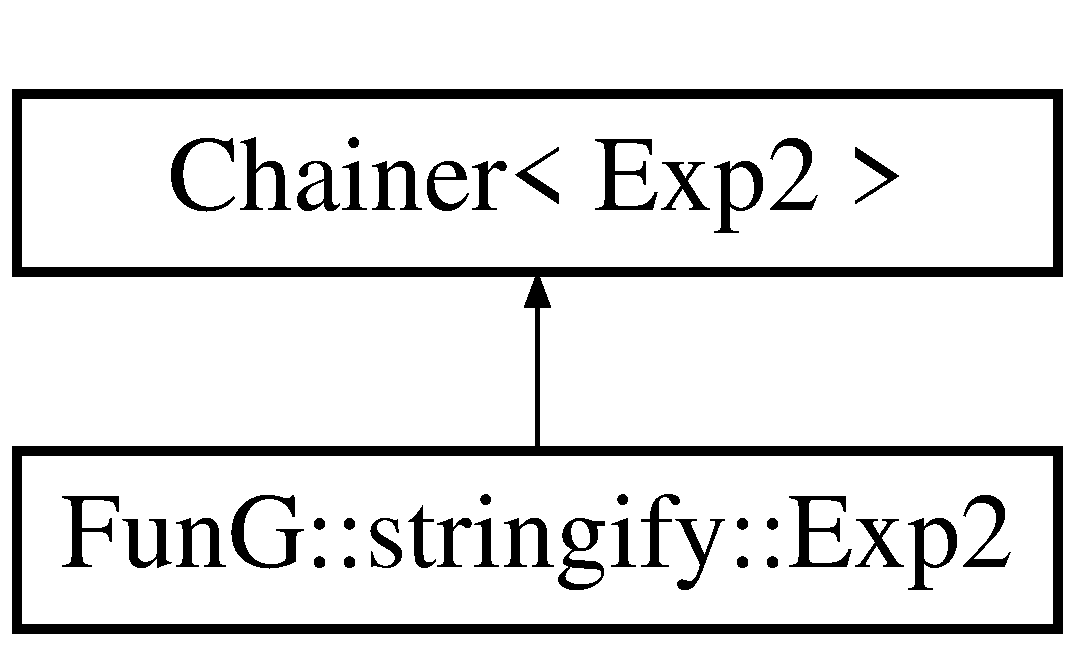
\includegraphics[height=2.000000cm]{structFunG_1_1stringify_1_1Exp2}
\end{center}
\end{figure}
\subsection*{Public Member Functions}
\begin{DoxyCompactItemize}
\item 
\hyperlink{structFunG_1_1stringify_1_1Exp2_ac3104f75c4473ff5276a3dcb1173c392}{Exp2} (const \hyperlink{structFunG_1_1String}{String} \&x=\char`\"{}x\char`\"{})
\begin{DoxyCompactList}\small\item\em Constructor. \end{DoxyCompactList}\item 
void \hyperlink{structFunG_1_1stringify_1_1Exp2_ada28d06b408c32cbae875d023f141dd5}{update} (const \hyperlink{structFunG_1_1String}{String} \&x)
\begin{DoxyCompactList}\small\item\em Set point of evaluation. \end{DoxyCompactList}\item 
\hyperlink{structFunG_1_1String}{String} \hyperlink{structFunG_1_1stringify_1_1Exp2_a1ccf37b27078775a4ffa5bdcb5b65d99}{d0} () const noexcept
\begin{DoxyCompactList}\small\item\em Function value. \end{DoxyCompactList}\item 
\hyperlink{structFunG_1_1String}{String} \hyperlink{structFunG_1_1stringify_1_1Exp2_ae0ecd0b0cb1b79fe6fae2c7647f27051}{d1} (const \hyperlink{structFunG_1_1String}{String} \&dx=\char`\"{}\char`\"{}) const 
\begin{DoxyCompactList}\small\item\em First (directional) derivative. \end{DoxyCompactList}\item 
\hyperlink{structFunG_1_1String}{String} \hyperlink{structFunG_1_1stringify_1_1Exp2_a69f8b39f66bf404130333d41394e4c94}{d2} (const \hyperlink{structFunG_1_1String}{String} \&dx=\char`\"{}\char`\"{}, const \hyperlink{structFunG_1_1String}{String} \&dy=\char`\"{}\char`\"{}) const 
\begin{DoxyCompactList}\small\item\em Second (directional) derivative. \end{DoxyCompactList}\item 
\hyperlink{structFunG_1_1String}{String} \hyperlink{structFunG_1_1stringify_1_1Exp2_a277ff60c6eece735943e690df73bf121}{d3} (const \hyperlink{structFunG_1_1String}{String} \&dx=\char`\"{}\char`\"{}, const \hyperlink{structFunG_1_1String}{String} \&dy=\char`\"{}\char`\"{}, const \hyperlink{structFunG_1_1String}{String} \&dz=\char`\"{}\char`\"{}) const 
\begin{DoxyCompactList}\small\item\em Third (directional) derivative. \end{DoxyCompactList}\end{DoxyCompactItemize}


\subsection{Detailed Description}
Function $2^x$ including first three derivatives. 

For scalar functions directional derivatives are less interesting. Incorporating this function as building block for more complex functions requires directional derivatives. These occur during applications of the chain rule. 

\subsection{Constructor \& Destructor Documentation}
\hypertarget{structFunG_1_1stringify_1_1Exp2_ac3104f75c4473ff5276a3dcb1173c392}{\index{Fun\-G\-::stringify\-::\-Exp2@{Fun\-G\-::stringify\-::\-Exp2}!Exp2@{Exp2}}
\index{Exp2@{Exp2}!FunG::stringify::Exp2@{Fun\-G\-::stringify\-::\-Exp2}}
\subsubsection[{Exp2}]{\setlength{\rightskip}{0pt plus 5cm}Fun\-G\-::stringify\-::\-Exp2\-::\-Exp2 (
\begin{DoxyParamCaption}
\item[{const {\bf String} \&}]{x = {\ttfamily \char`\"{}x\char`\"{}}}
\end{DoxyParamCaption}
)\hspace{0.3cm}{\ttfamily [inline]}, {\ttfamily [explicit]}}}\label{structFunG_1_1stringify_1_1Exp2_ac3104f75c4473ff5276a3dcb1173c392}


Constructor. 


\begin{DoxyParams}{Parameters}
{\em x} & point of evaluation \\
\hline
\end{DoxyParams}


\subsection{Member Function Documentation}
\hypertarget{structFunG_1_1stringify_1_1Exp2_a1ccf37b27078775a4ffa5bdcb5b65d99}{\index{Fun\-G\-::stringify\-::\-Exp2@{Fun\-G\-::stringify\-::\-Exp2}!d0@{d0}}
\index{d0@{d0}!FunG::stringify::Exp2@{Fun\-G\-::stringify\-::\-Exp2}}
\subsubsection[{d0}]{\setlength{\rightskip}{0pt plus 5cm}{\bf String} Fun\-G\-::stringify\-::\-Exp2\-::d0 (
\begin{DoxyParamCaption}
{}
\end{DoxyParamCaption}
) const\hspace{0.3cm}{\ttfamily [inline]}, {\ttfamily [noexcept]}}}\label{structFunG_1_1stringify_1_1Exp2_a1ccf37b27078775a4ffa5bdcb5b65d99}


Function value. 

\hypertarget{structFunG_1_1stringify_1_1Exp2_ae0ecd0b0cb1b79fe6fae2c7647f27051}{\index{Fun\-G\-::stringify\-::\-Exp2@{Fun\-G\-::stringify\-::\-Exp2}!d1@{d1}}
\index{d1@{d1}!FunG::stringify::Exp2@{Fun\-G\-::stringify\-::\-Exp2}}
\subsubsection[{d1}]{\setlength{\rightskip}{0pt plus 5cm}{\bf String} Fun\-G\-::stringify\-::\-Exp2\-::d1 (
\begin{DoxyParamCaption}
\item[{const {\bf String} \&}]{dx = {\ttfamily \char`\"{}\char`\"{}}}
\end{DoxyParamCaption}
) const\hspace{0.3cm}{\ttfamily [inline]}}}\label{structFunG_1_1stringify_1_1Exp2_ae0ecd0b0cb1b79fe6fae2c7647f27051}


First (directional) derivative. 

\hypertarget{structFunG_1_1stringify_1_1Exp2_a69f8b39f66bf404130333d41394e4c94}{\index{Fun\-G\-::stringify\-::\-Exp2@{Fun\-G\-::stringify\-::\-Exp2}!d2@{d2}}
\index{d2@{d2}!FunG::stringify::Exp2@{Fun\-G\-::stringify\-::\-Exp2}}
\subsubsection[{d2}]{\setlength{\rightskip}{0pt plus 5cm}{\bf String} Fun\-G\-::stringify\-::\-Exp2\-::d2 (
\begin{DoxyParamCaption}
\item[{const {\bf String} \&}]{dx = {\ttfamily \char`\"{}\char`\"{}}, }
\item[{const {\bf String} \&}]{dy = {\ttfamily \char`\"{}\char`\"{}}}
\end{DoxyParamCaption}
) const\hspace{0.3cm}{\ttfamily [inline]}}}\label{structFunG_1_1stringify_1_1Exp2_a69f8b39f66bf404130333d41394e4c94}


Second (directional) derivative. 

\hypertarget{structFunG_1_1stringify_1_1Exp2_a277ff60c6eece735943e690df73bf121}{\index{Fun\-G\-::stringify\-::\-Exp2@{Fun\-G\-::stringify\-::\-Exp2}!d3@{d3}}
\index{d3@{d3}!FunG::stringify::Exp2@{Fun\-G\-::stringify\-::\-Exp2}}
\subsubsection[{d3}]{\setlength{\rightskip}{0pt plus 5cm}{\bf String} Fun\-G\-::stringify\-::\-Exp2\-::d3 (
\begin{DoxyParamCaption}
\item[{const {\bf String} \&}]{dx = {\ttfamily \char`\"{}\char`\"{}}, }
\item[{const {\bf String} \&}]{dy = {\ttfamily \char`\"{}\char`\"{}}, }
\item[{const {\bf String} \&}]{dz = {\ttfamily \char`\"{}\char`\"{}}}
\end{DoxyParamCaption}
) const\hspace{0.3cm}{\ttfamily [inline]}}}\label{structFunG_1_1stringify_1_1Exp2_a277ff60c6eece735943e690df73bf121}


Third (directional) derivative. 

\hypertarget{structFunG_1_1stringify_1_1Exp2_ada28d06b408c32cbae875d023f141dd5}{\index{Fun\-G\-::stringify\-::\-Exp2@{Fun\-G\-::stringify\-::\-Exp2}!update@{update}}
\index{update@{update}!FunG::stringify::Exp2@{Fun\-G\-::stringify\-::\-Exp2}}
\subsubsection[{update}]{\setlength{\rightskip}{0pt plus 5cm}void Fun\-G\-::stringify\-::\-Exp2\-::update (
\begin{DoxyParamCaption}
\item[{const {\bf String} \&}]{x}
\end{DoxyParamCaption}
)\hspace{0.3cm}{\ttfamily [inline]}}}\label{structFunG_1_1stringify_1_1Exp2_ada28d06b408c32cbae875d023f141dd5}


Set point of evaluation. 



The documentation for this struct was generated from the following file\-:\begin{DoxyCompactItemize}
\item 
include/fung/cmath/stringify/\hyperlink{stringify_2exp_8hh}{exp.\-hh}\end{DoxyCompactItemize}

\hypertarget{structFunG_1_1LinearAlgebra_1_1ExtractDimension}{\section{\-Fun\-G\-:\-:\-Linear\-Algebra\-:\-:\-Extract\-Dimension$<$ \-Matrix, class $>$ \-Struct \-Template \-Reference}
\label{structFunG_1_1LinearAlgebra_1_1ExtractDimension}\index{\-Fun\-G\-::\-Linear\-Algebra\-::\-Extract\-Dimension$<$ Matrix, class $>$@{\-Fun\-G\-::\-Linear\-Algebra\-::\-Extract\-Dimension$<$ Matrix, class $>$}}
}


\-Specialize this for your matrix class. \-Dimension (number of rows/columns for square matrices) must be provided by a static member variable called value.  




{\ttfamily \#include $<$dimension.\-hh$>$}

\-Inheritance diagram for \-Fun\-G\-:\-:\-Linear\-Algebra\-:\-:\-Extract\-Dimension$<$ \-Matrix, class $>$\-:\begin{figure}[H]
\begin{center}
\leavevmode
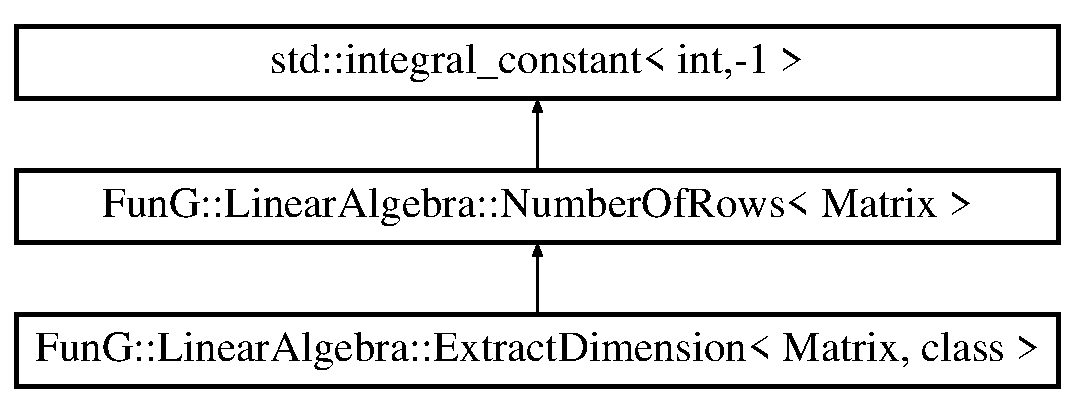
\includegraphics[height=3.000000cm]{structFunG_1_1LinearAlgebra_1_1ExtractDimension}
\end{center}
\end{figure}


\subsection{\-Detailed \-Description}
\subsubsection*{template$<$class Matrix, class = \-Concepts\-::\-Square\-Matrix\-Concept\-Check$<$\-Matrix$>$$>$struct Fun\-G\-::\-Linear\-Algebra\-::\-Extract\-Dimension$<$ Matrix, class $>$}

\-Specialize this for your matrix class. \-Dimension (number of rows/columns for square matrices) must be provided by a static member variable called value. 

\-The documentation for this struct was generated from the following file\-:\begin{DoxyCompactItemize}
\item 
fung/linear\-\_\-algebra/\hyperlink{dimension_8hh}{dimension.\-hh}\end{DoxyCompactItemize}

\hypertarget{structFunG_1_1Concepts_1_1FunctionConcept}{\section{Fun\-G\-:\-:Concepts\-:\-:Function\-Concept Struct Reference}
\label{structFunG_1_1Concepts_1_1FunctionConcept}\index{Fun\-G\-::\-Concepts\-::\-Function\-Concept@{Fun\-G\-::\-Concepts\-::\-Function\-Concept}}
}


Minimal requirements for functions.  




{\ttfamily \#include $<$concepts.\-hh$>$}

Inheritance diagram for Fun\-G\-:\-:Concepts\-:\-:Function\-Concept\-:\begin{figure}[H]
\begin{center}
\leavevmode
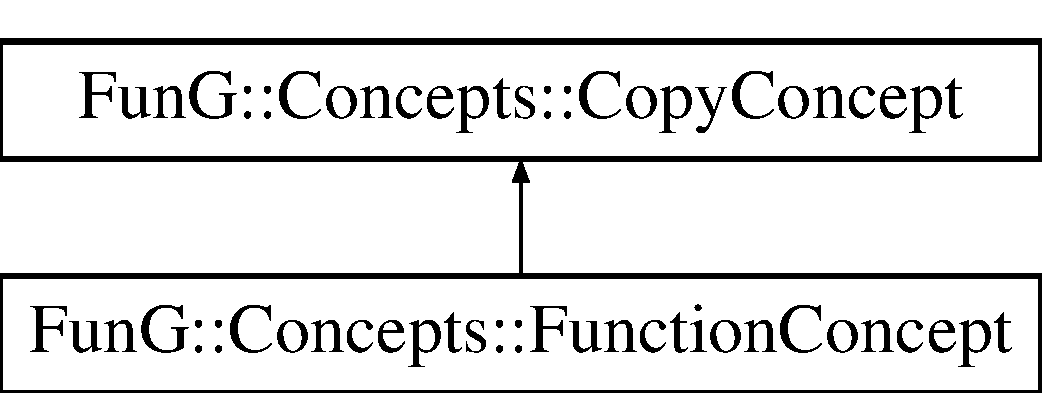
\includegraphics[height=2.000000cm]{structFunG_1_1Concepts_1_1FunctionConcept}
\end{center}
\end{figure}
\subsection*{Public Member Functions}
\begin{DoxyCompactItemize}
\item 
\hypertarget{structFunG_1_1Concepts_1_1FunctionConcept_a3ced15c8956956bd12c2776fc7c79771}{unspecified \hyperlink{structFunG_1_1Concepts_1_1FunctionConcept_a3ced15c8956956bd12c2776fc7c79771}{d0} () const }\label{structFunG_1_1Concepts_1_1FunctionConcept_a3ced15c8956956bd12c2776fc7c79771}

\begin{DoxyCompactList}\small\item\em Access to function value. \end{DoxyCompactList}\end{DoxyCompactItemize}


\subsection{Detailed Description}
Minimal requirements for functions. 

The documentation for this struct was generated from the following file\-:\begin{DoxyCompactItemize}
\item 
Fun\-G/\hyperlink{concepts_8hh}{concepts.\-hh}\end{DoxyCompactItemize}

\hypertarget{structFunG_1_1Concepts_1_1FunctionConceptCheck}{}\section{Fun\+G\+:\+:Concepts\+:\+:Function\+Concept\+Check$<$ F $>$ Struct Template Reference}
\label{structFunG_1_1Concepts_1_1FunctionConceptCheck}\index{Fun\+G\+::\+Concepts\+::\+Function\+Concept\+Check$<$ F $>$@{Fun\+G\+::\+Concepts\+::\+Function\+Concept\+Check$<$ F $>$}}


Static check if the requirements of \hyperlink{structFunG_1_1Concepts_1_1FunctionConcept}{Function\+Concept} are satisfied.  




{\ttfamily \#include $<$concept\+\_\+check.\+hh$>$}

Inheritance diagram for Fun\+G\+:\+:Concepts\+:\+:Function\+Concept\+Check$<$ F $>$\+:\begin{figure}[H]
\begin{center}
\leavevmode
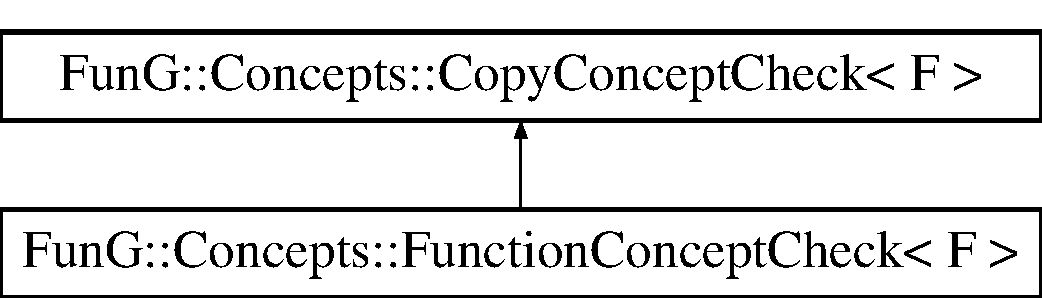
\includegraphics[height=2.000000cm]{structFunG_1_1Concepts_1_1FunctionConceptCheck}
\end{center}
\end{figure}


\subsection{Detailed Description}
\subsubsection*{template$<$class F$>$struct Fun\+G\+::\+Concepts\+::\+Function\+Concept\+Check$<$ F $>$}

Static check if the requirements of \hyperlink{structFunG_1_1Concepts_1_1FunctionConcept}{Function\+Concept} are satisfied. 

The documentation for this struct was generated from the following file\+:\begin{DoxyCompactItemize}
\item 
fung/\hyperlink{concept__check_8hh}{concept\+\_\+check.\+hh}\end{DoxyCompactItemize}

\hypertarget{structFunG_1_1Identity}{}\section{FunG\+:\+:Identity$<$ Arg, class $>$ Struct Template Reference}
\label{structFunG_1_1Identity}\index{Fun\+G\+::\+Identity$<$ Arg, class $>$@{Fun\+G\+::\+Identity$<$ Arg, class $>$}}


Identity mapping $ f(x)=x $.  




{\ttfamily \#include $<$identity.\+hh$>$}

Inheritance diagram for FunG\+:\+:Identity$<$ Arg, class $>$\+:\begin{figure}[H]
\begin{center}
\leavevmode
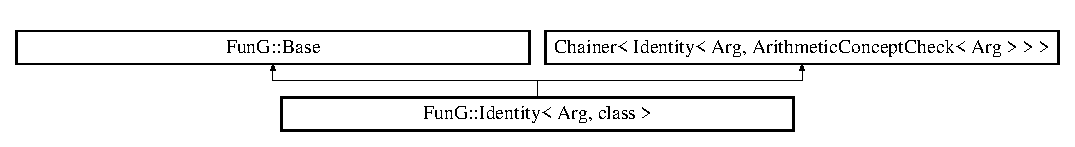
\includegraphics[height=2.000000cm]{structFunG_1_1Identity}
\end{center}
\end{figure}
\subsection*{Public Member Functions}
\begin{DoxyCompactItemize}
\item 
\hyperlink{structFunG_1_1Identity_a2480f818e33371734d328558f71248ec}{Identity} ()=default
\begin{DoxyCompactList}\small\item\em Default constructor. \end{DoxyCompactList}\item 
\hyperlink{structFunG_1_1Identity_a080e9bf064c469a5141765f3ee0416b0}{Identity} (const Arg \&x)
\begin{DoxyCompactList}\small\item\em Constructor. \end{DoxyCompactList}\item 
void \hyperlink{structFunG_1_1Identity_acceedd6198948c7e1eb782f7a358a759}{update} (const Arg \&x)
\begin{DoxyCompactList}\small\item\em Reset point of evaluation. \end{DoxyCompactList}\item 
const Arg \& \hyperlink{structFunG_1_1Identity_ab1edf393c23ed1bef1d3d84c28289e36}{d0} () const noexcept
\begin{DoxyCompactList}\small\item\em Function value. \end{DoxyCompactList}\item 
{\footnotesize template$<$int $>$ }\\const Arg \& \hyperlink{structFunG_1_1Identity_a9f22755ffd38fa5712446c0120deea21}{d1} (const Arg \&dx) const noexcept
\begin{DoxyCompactList}\small\item\em First directional derivative. \end{DoxyCompactList}\end{DoxyCompactItemize}


\subsection{Detailed Description}
\subsubsection*{template$<$class Arg, class = Arithmetic\+Concept\+Check$<$\+Arg$>$$>$\\*
struct Fun\+G\+::\+Identity$<$ Arg, class $>$}

Identity mapping $ f(x)=x $. 

\subsection{Constructor \& Destructor Documentation}
\index{Fun\+G\+::\+Identity@{Fun\+G\+::\+Identity}!Identity@{Identity}}
\index{Identity@{Identity}!Fun\+G\+::\+Identity@{Fun\+G\+::\+Identity}}
\subsubsection[{\texorpdfstring{Identity()=default}{Identity()=default}}]{\setlength{\rightskip}{0pt plus 5cm}template$<$class Arg , class  = Arithmetic\+Concept\+Check$<$\+Arg$>$$>$ {\bf Fun\+G\+::\+Identity}$<$ Arg, class $>$\+::{\bf Identity} (
\begin{DoxyParamCaption}
{}
\end{DoxyParamCaption}
)\hspace{0.3cm}{\ttfamily [default]}}\hypertarget{structFunG_1_1Identity_a2480f818e33371734d328558f71248ec}{}\label{structFunG_1_1Identity_a2480f818e33371734d328558f71248ec}


Default constructor. 

\index{Fun\+G\+::\+Identity@{Fun\+G\+::\+Identity}!Identity@{Identity}}
\index{Identity@{Identity}!Fun\+G\+::\+Identity@{Fun\+G\+::\+Identity}}
\subsubsection[{\texorpdfstring{Identity(const Arg \&x)}{Identity(const Arg &x)}}]{\setlength{\rightskip}{0pt plus 5cm}template$<$class Arg , class  = Arithmetic\+Concept\+Check$<$\+Arg$>$$>$ {\bf Fun\+G\+::\+Identity}$<$ Arg, class $>$\+::{\bf Identity} (
\begin{DoxyParamCaption}
\item[{const Arg \&}]{x}
\end{DoxyParamCaption}
)\hspace{0.3cm}{\ttfamily [inline]}}\hypertarget{structFunG_1_1Identity_a080e9bf064c469a5141765f3ee0416b0}{}\label{structFunG_1_1Identity_a080e9bf064c469a5141765f3ee0416b0}


Constructor. 


\begin{DoxyParams}{Parameters}
{\em x} & point of evaluation. \\
\hline
\end{DoxyParams}


\subsection{Member Function Documentation}
\index{Fun\+G\+::\+Identity@{Fun\+G\+::\+Identity}!d0@{d0}}
\index{d0@{d0}!Fun\+G\+::\+Identity@{Fun\+G\+::\+Identity}}
\subsubsection[{\texorpdfstring{d0() const noexcept}{d0() const noexcept}}]{\setlength{\rightskip}{0pt plus 5cm}template$<$class Arg , class  = Arithmetic\+Concept\+Check$<$\+Arg$>$$>$ const Arg\& {\bf Fun\+G\+::\+Identity}$<$ Arg, class $>$\+::d0 (
\begin{DoxyParamCaption}
{}
\end{DoxyParamCaption}
) const\hspace{0.3cm}{\ttfamily [inline]}, {\ttfamily [noexcept]}}\hypertarget{structFunG_1_1Identity_ab1edf393c23ed1bef1d3d84c28289e36}{}\label{structFunG_1_1Identity_ab1edf393c23ed1bef1d3d84c28289e36}


Function value. 

\index{Fun\+G\+::\+Identity@{Fun\+G\+::\+Identity}!d1@{d1}}
\index{d1@{d1}!Fun\+G\+::\+Identity@{Fun\+G\+::\+Identity}}
\subsubsection[{\texorpdfstring{d1(const Arg \&dx) const noexcept}{d1(const Arg &dx) const noexcept}}]{\setlength{\rightskip}{0pt plus 5cm}template$<$class Arg , class  = Arithmetic\+Concept\+Check$<$\+Arg$>$$>$ template$<$int $>$ const Arg\& {\bf Fun\+G\+::\+Identity}$<$ Arg, class $>$\+::d1 (
\begin{DoxyParamCaption}
\item[{const Arg \&}]{dx}
\end{DoxyParamCaption}
) const\hspace{0.3cm}{\ttfamily [inline]}, {\ttfamily [noexcept]}}\hypertarget{structFunG_1_1Identity_a9f22755ffd38fa5712446c0120deea21}{}\label{structFunG_1_1Identity_a9f22755ffd38fa5712446c0120deea21}


First directional derivative. 

\index{Fun\+G\+::\+Identity@{Fun\+G\+::\+Identity}!update@{update}}
\index{update@{update}!Fun\+G\+::\+Identity@{Fun\+G\+::\+Identity}}
\subsubsection[{\texorpdfstring{update(const Arg \&x)}{update(const Arg &x)}}]{\setlength{\rightskip}{0pt plus 5cm}template$<$class Arg , class  = Arithmetic\+Concept\+Check$<$\+Arg$>$$>$ void {\bf Fun\+G\+::\+Identity}$<$ Arg, class $>$\+::update (
\begin{DoxyParamCaption}
\item[{const Arg \&}]{x}
\end{DoxyParamCaption}
)\hspace{0.3cm}{\ttfamily [inline]}}\hypertarget{structFunG_1_1Identity_acceedd6198948c7e1eb782f7a358a759}{}\label{structFunG_1_1Identity_acceedd6198948c7e1eb782f7a358a759}


Reset point of evaluation. 



The documentation for this struct was generated from the following file\+:\begin{DoxyCompactItemize}
\item 
include/fung/\hyperlink{identity_8hh}{identity.\+hh}\end{DoxyCompactItemize}

\hypertarget{structFunG_1_1is__arithmetic}{\section{Fun\-G\-:\-:is\-\_\-arithmetic$<$ F $>$ Struct Template Reference}
\label{structFunG_1_1is__arithmetic}\index{Fun\-G\-::is\-\_\-arithmetic$<$ F $>$@{Fun\-G\-::is\-\_\-arithmetic$<$ F $>$}}
}


Specialize this template class to register arithmetic types that are not built-\/in.  




{\ttfamily \#include $<$type\-\_\-traits.\-hh$>$}

Inheritance diagram for Fun\-G\-:\-:is\-\_\-arithmetic$<$ F $>$\-:\begin{figure}[H]
\begin{center}
\leavevmode
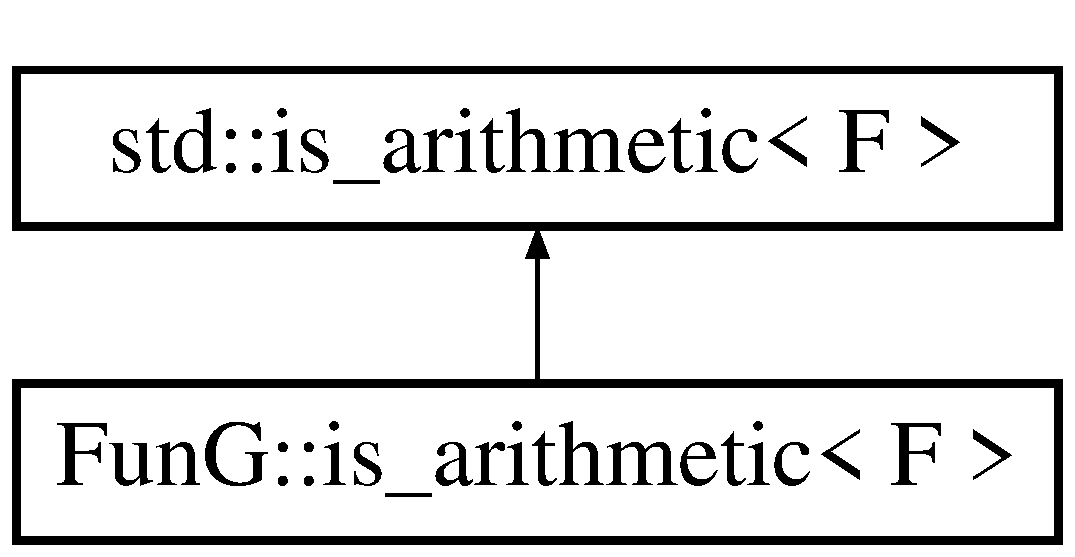
\includegraphics[height=2.000000cm]{structFunG_1_1is__arithmetic}
\end{center}
\end{figure}


\subsection{Detailed Description}
\subsubsection*{template$<$class F$>$struct Fun\-G\-::is\-\_\-arithmetic$<$ F $>$}

Specialize this template class to register arithmetic types that are not built-\/in. 

The documentation for this struct was generated from the following file\-:\begin{DoxyCompactItemize}
\item 
include/fung/util/\hyperlink{type__traits_8hh}{type\-\_\-traits.\-hh}\end{DoxyCompactItemize}

\hypertarget{classFunG_1_1LinearAlgebra_1_1LeftCauchyGreenStrainTensor}{\section{Fun\-G\-:\-:Linear\-Algebra\-:\-:Left\-Cauchy\-Green\-Strain\-Tensor$<$ Matrix, class $>$ Class Template Reference}
\label{classFunG_1_1LinearAlgebra_1_1LeftCauchyGreenStrainTensor}\index{Fun\-G\-::\-Linear\-Algebra\-::\-Left\-Cauchy\-Green\-Strain\-Tensor$<$ Matrix, class $>$@{Fun\-G\-::\-Linear\-Algebra\-::\-Left\-Cauchy\-Green\-Strain\-Tensor$<$ Matrix, class $>$}}
}


Left Cauchy-\/\-Green strain tensor $ F^T F $ for a symmetric matrix $ F $.  




{\ttfamily \#include $<$strain\-Tensor.\-hh$>$}

Inheritance diagram for Fun\-G\-:\-:Linear\-Algebra\-:\-:Left\-Cauchy\-Green\-Strain\-Tensor$<$ Matrix, class $>$\-:\begin{figure}[H]
\begin{center}
\leavevmode
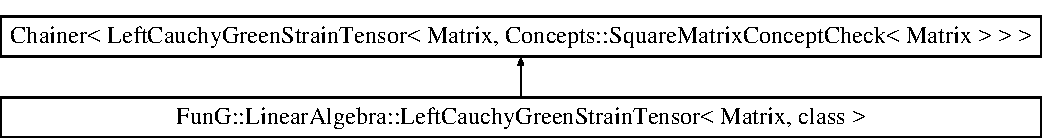
\includegraphics[height=0.898876cm]{classFunG_1_1LinearAlgebra_1_1LeftCauchyGreenStrainTensor}
\end{center}
\end{figure}
\subsection*{Public Member Functions}
\begin{DoxyCompactItemize}
\item 
\hyperlink{classFunG_1_1LinearAlgebra_1_1LeftCauchyGreenStrainTensor_a6bfc0f686be29024dc740630f364d051}{Left\-Cauchy\-Green\-Strain\-Tensor} (Matrix const \&F)
\begin{DoxyCompactList}\small\item\em Constructor. \end{DoxyCompactList}\item 
\hypertarget{classFunG_1_1LinearAlgebra_1_1LeftCauchyGreenStrainTensor_a3ab24c88bf4e9f9240dee4544027c238}{void \hyperlink{classFunG_1_1LinearAlgebra_1_1LeftCauchyGreenStrainTensor_a3ab24c88bf4e9f9240dee4544027c238}{update} (Matrix const \&F)}\label{classFunG_1_1LinearAlgebra_1_1LeftCauchyGreenStrainTensor_a3ab24c88bf4e9f9240dee4544027c238}

\begin{DoxyCompactList}\small\item\em Reset point of evaluation. \end{DoxyCompactList}\item 
\hypertarget{classFunG_1_1LinearAlgebra_1_1LeftCauchyGreenStrainTensor_a541f165ca20f61eeae1b5cf2d6bc42c6}{Matrix const \& \hyperlink{classFunG_1_1LinearAlgebra_1_1LeftCauchyGreenStrainTensor_a541f165ca20f61eeae1b5cf2d6bc42c6}{d0} () const noexcept}\label{classFunG_1_1LinearAlgebra_1_1LeftCauchyGreenStrainTensor_a541f165ca20f61eeae1b5cf2d6bc42c6}

\begin{DoxyCompactList}\small\item\em Function value $ F^T * F $. \end{DoxyCompactList}\item 
\hypertarget{classFunG_1_1LinearAlgebra_1_1LeftCauchyGreenStrainTensor_ae61332db7d9941efd055273c6f00af6f}{{\footnotesize template$<$int $>$ }\\Matrix \hyperlink{classFunG_1_1LinearAlgebra_1_1LeftCauchyGreenStrainTensor_ae61332db7d9941efd055273c6f00af6f}{d1} (Matrix const \&d\-F1) const }\label{classFunG_1_1LinearAlgebra_1_1LeftCauchyGreenStrainTensor_ae61332db7d9941efd055273c6f00af6f}

\begin{DoxyCompactList}\small\item\em First directional derivative $ F^T dF_1 + dF_1^T F $. \end{DoxyCompactList}\item 
\hypertarget{classFunG_1_1LinearAlgebra_1_1LeftCauchyGreenStrainTensor_a5ad1ba43d88d878f5236b55d86bddb11}{{\footnotesize template$<$int , int $>$ }\\Matrix \hyperlink{classFunG_1_1LinearAlgebra_1_1LeftCauchyGreenStrainTensor_a5ad1ba43d88d878f5236b55d86bddb11}{d2} (Matrix const \&d\-F1, Matrix const \&d\-F2) const }\label{classFunG_1_1LinearAlgebra_1_1LeftCauchyGreenStrainTensor_a5ad1ba43d88d878f5236b55d86bddb11}

\begin{DoxyCompactList}\small\item\em Second directional derivative $ dF_2^T dF_1 + dF_1^T dF_2 $. \end{DoxyCompactList}\end{DoxyCompactItemize}


\subsection{Detailed Description}
\subsubsection*{template$<$class Matrix, class = Concepts\-::\-Symmetric\-Matrix\-Concept\-Check$<$\-Matrix$>$$>$class Fun\-G\-::\-Linear\-Algebra\-::\-Left\-Cauchy\-Green\-Strain\-Tensor$<$ Matrix, class $>$}

Left Cauchy-\/\-Green strain tensor $ F^T F $ for a symmetric matrix $ F $. 

This class is used for nonlinear material models based on the deformation gradient $\nabla\varphi$, which takes the role of $F$. Caches both $ F^T $ and $ F^T F $. 

\subsection{Constructor \& Destructor Documentation}
\hypertarget{classFunG_1_1LinearAlgebra_1_1LeftCauchyGreenStrainTensor_a6bfc0f686be29024dc740630f364d051}{\index{Fun\-G\-::\-Linear\-Algebra\-::\-Left\-Cauchy\-Green\-Strain\-Tensor@{Fun\-G\-::\-Linear\-Algebra\-::\-Left\-Cauchy\-Green\-Strain\-Tensor}!Left\-Cauchy\-Green\-Strain\-Tensor@{Left\-Cauchy\-Green\-Strain\-Tensor}}
\index{Left\-Cauchy\-Green\-Strain\-Tensor@{Left\-Cauchy\-Green\-Strain\-Tensor}!FunG::LinearAlgebra::LeftCauchyGreenStrainTensor@{Fun\-G\-::\-Linear\-Algebra\-::\-Left\-Cauchy\-Green\-Strain\-Tensor}}
\subsubsection[{Left\-Cauchy\-Green\-Strain\-Tensor}]{\setlength{\rightskip}{0pt plus 5cm}template$<$class Matrix , class  = Concepts\-::\-Symmetric\-Matrix\-Concept\-Check$<$\-Matrix$>$$>$ {\bf Fun\-G\-::\-Linear\-Algebra\-::\-Left\-Cauchy\-Green\-Strain\-Tensor}$<$ Matrix, class $>$\-::{\bf Left\-Cauchy\-Green\-Strain\-Tensor} (
\begin{DoxyParamCaption}
\item[{Matrix const \&}]{F}
\end{DoxyParamCaption}
)\hspace{0.3cm}{\ttfamily [inline]}, {\ttfamily [explicit]}}}\label{classFunG_1_1LinearAlgebra_1_1LeftCauchyGreenStrainTensor_a6bfc0f686be29024dc740630f364d051}


Constructor. 


\begin{DoxyParams}{Parameters}
{\em F} & point of evaluation. \\
\hline
\end{DoxyParams}


The documentation for this class was generated from the following file\-:\begin{DoxyCompactItemize}
\item 
Fun\-G/\-Linear\-Algebra/strain\-Tensor.\-hh\end{DoxyCompactItemize}

\hypertarget{structFunG_1_1stringify_1_1LN}{\section{Fun\-G\-:\-:stringify\-:\-:L\-N Struct Reference}
\label{structFunG_1_1stringify_1_1LN}\index{Fun\-G\-::stringify\-::\-L\-N@{Fun\-G\-::stringify\-::\-L\-N}}
}


{\ttfamily \#include $<$log.\-hh$>$}

Inheritance diagram for Fun\-G\-:\-:stringify\-:\-:L\-N\-:\begin{figure}[H]
\begin{center}
\leavevmode
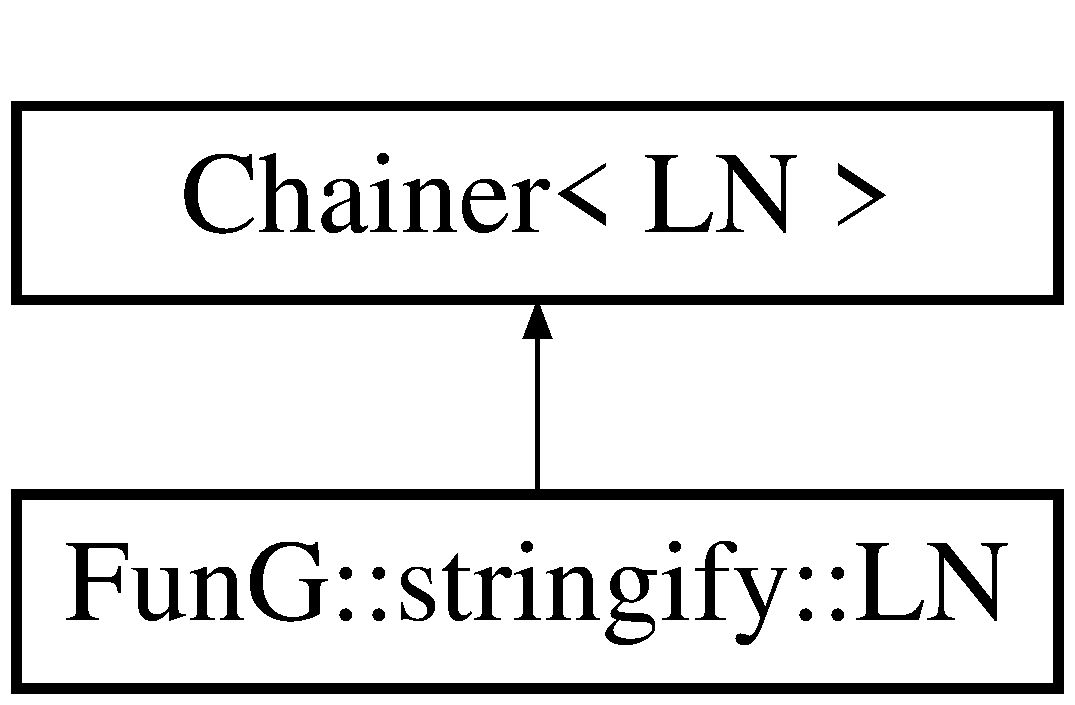
\includegraphics[height=2.000000cm]{structFunG_1_1stringify_1_1LN}
\end{center}
\end{figure}
\subsection*{Public Member Functions}
\begin{DoxyCompactItemize}
\item 
\hyperlink{structFunG_1_1stringify_1_1LN_a27f182c8cc57cebe4b0463ed276d119e}{L\-N} (const \hyperlink{structFunG_1_1String}{String} \&x=\char`\"{}x\char`\"{})
\begin{DoxyCompactList}\small\item\em Constructor. \end{DoxyCompactList}\item 
void \hyperlink{structFunG_1_1stringify_1_1LN_aa350fa6848e94377ca4c985a440445e3}{update} (const \hyperlink{structFunG_1_1String}{String} \&x)
\begin{DoxyCompactList}\small\item\em Set point of evaluation. \end{DoxyCompactList}\item 
\hyperlink{structFunG_1_1String}{String} \hyperlink{structFunG_1_1stringify_1_1LN_abea0b27e81113e4bfb5acdb5073182cd}{d0} () const noexcept
\begin{DoxyCompactList}\small\item\em Function value. \end{DoxyCompactList}\item 
\hyperlink{structFunG_1_1String}{String} \hyperlink{structFunG_1_1stringify_1_1LN_af9705c416c225c0ebd78316444ab26c4}{d1} (const \hyperlink{structFunG_1_1String}{String} \&dx=\char`\"{}\char`\"{}) const 
\begin{DoxyCompactList}\small\item\em First (directional) derivative. \end{DoxyCompactList}\item 
\hyperlink{structFunG_1_1String}{String} \hyperlink{structFunG_1_1stringify_1_1LN_a1379edb471691b5ab6b34701896033ae}{d2} (const \hyperlink{structFunG_1_1String}{String} \&dx=\char`\"{}\char`\"{}, const \hyperlink{structFunG_1_1String}{String} \&dy=\char`\"{}\char`\"{}) const 
\begin{DoxyCompactList}\small\item\em Second (directional) derivative. \end{DoxyCompactList}\item 
\hyperlink{structFunG_1_1String}{String} \hyperlink{structFunG_1_1stringify_1_1LN_aeeabb2c2cc220b6350ac1040b879086b}{d3} (const \hyperlink{structFunG_1_1String}{String} \&dx=\char`\"{}\char`\"{}, const \hyperlink{structFunG_1_1String}{String} \&dy=\char`\"{}\char`\"{}, const \hyperlink{structFunG_1_1String}{String} \&dz=\char`\"{}\char`\"{}) const 
\begin{DoxyCompactList}\small\item\em Third (directional) derivative. \end{DoxyCompactList}\end{DoxyCompactItemize}


\subsection{Constructor \& Destructor Documentation}
\hypertarget{structFunG_1_1stringify_1_1LN_a27f182c8cc57cebe4b0463ed276d119e}{\index{Fun\-G\-::stringify\-::\-L\-N@{Fun\-G\-::stringify\-::\-L\-N}!L\-N@{L\-N}}
\index{L\-N@{L\-N}!FunG::stringify::LN@{Fun\-G\-::stringify\-::\-L\-N}}
\subsubsection[{L\-N}]{\setlength{\rightskip}{0pt plus 5cm}Fun\-G\-::stringify\-::\-L\-N\-::\-L\-N (
\begin{DoxyParamCaption}
\item[{const {\bf String} \&}]{x = {\ttfamily \char`\"{}x\char`\"{}}}
\end{DoxyParamCaption}
)\hspace{0.3cm}{\ttfamily [inline]}, {\ttfamily [explicit]}}}\label{structFunG_1_1stringify_1_1LN_a27f182c8cc57cebe4b0463ed276d119e}


Constructor. 


\begin{DoxyParams}{Parameters}
{\em x} & point of evaluation \\
\hline
\end{DoxyParams}


\subsection{Member Function Documentation}
\hypertarget{structFunG_1_1stringify_1_1LN_abea0b27e81113e4bfb5acdb5073182cd}{\index{Fun\-G\-::stringify\-::\-L\-N@{Fun\-G\-::stringify\-::\-L\-N}!d0@{d0}}
\index{d0@{d0}!FunG::stringify::LN@{Fun\-G\-::stringify\-::\-L\-N}}
\subsubsection[{d0}]{\setlength{\rightskip}{0pt plus 5cm}{\bf String} Fun\-G\-::stringify\-::\-L\-N\-::d0 (
\begin{DoxyParamCaption}
{}
\end{DoxyParamCaption}
) const\hspace{0.3cm}{\ttfamily [inline]}, {\ttfamily [noexcept]}}}\label{structFunG_1_1stringify_1_1LN_abea0b27e81113e4bfb5acdb5073182cd}


Function value. 

\hypertarget{structFunG_1_1stringify_1_1LN_af9705c416c225c0ebd78316444ab26c4}{\index{Fun\-G\-::stringify\-::\-L\-N@{Fun\-G\-::stringify\-::\-L\-N}!d1@{d1}}
\index{d1@{d1}!FunG::stringify::LN@{Fun\-G\-::stringify\-::\-L\-N}}
\subsubsection[{d1}]{\setlength{\rightskip}{0pt plus 5cm}{\bf String} Fun\-G\-::stringify\-::\-L\-N\-::d1 (
\begin{DoxyParamCaption}
\item[{const {\bf String} \&}]{dx = {\ttfamily \char`\"{}\char`\"{}}}
\end{DoxyParamCaption}
) const\hspace{0.3cm}{\ttfamily [inline]}}}\label{structFunG_1_1stringify_1_1LN_af9705c416c225c0ebd78316444ab26c4}


First (directional) derivative. 

\hypertarget{structFunG_1_1stringify_1_1LN_a1379edb471691b5ab6b34701896033ae}{\index{Fun\-G\-::stringify\-::\-L\-N@{Fun\-G\-::stringify\-::\-L\-N}!d2@{d2}}
\index{d2@{d2}!FunG::stringify::LN@{Fun\-G\-::stringify\-::\-L\-N}}
\subsubsection[{d2}]{\setlength{\rightskip}{0pt plus 5cm}{\bf String} Fun\-G\-::stringify\-::\-L\-N\-::d2 (
\begin{DoxyParamCaption}
\item[{const {\bf String} \&}]{dx = {\ttfamily \char`\"{}\char`\"{}}, }
\item[{const {\bf String} \&}]{dy = {\ttfamily \char`\"{}\char`\"{}}}
\end{DoxyParamCaption}
) const\hspace{0.3cm}{\ttfamily [inline]}}}\label{structFunG_1_1stringify_1_1LN_a1379edb471691b5ab6b34701896033ae}


Second (directional) derivative. 

\hypertarget{structFunG_1_1stringify_1_1LN_aeeabb2c2cc220b6350ac1040b879086b}{\index{Fun\-G\-::stringify\-::\-L\-N@{Fun\-G\-::stringify\-::\-L\-N}!d3@{d3}}
\index{d3@{d3}!FunG::stringify::LN@{Fun\-G\-::stringify\-::\-L\-N}}
\subsubsection[{d3}]{\setlength{\rightskip}{0pt plus 5cm}{\bf String} Fun\-G\-::stringify\-::\-L\-N\-::d3 (
\begin{DoxyParamCaption}
\item[{const {\bf String} \&}]{dx = {\ttfamily \char`\"{}\char`\"{}}, }
\item[{const {\bf String} \&}]{dy = {\ttfamily \char`\"{}\char`\"{}}, }
\item[{const {\bf String} \&}]{dz = {\ttfamily \char`\"{}\char`\"{}}}
\end{DoxyParamCaption}
) const\hspace{0.3cm}{\ttfamily [inline]}}}\label{structFunG_1_1stringify_1_1LN_aeeabb2c2cc220b6350ac1040b879086b}


Third (directional) derivative. 

\hypertarget{structFunG_1_1stringify_1_1LN_aa350fa6848e94377ca4c985a440445e3}{\index{Fun\-G\-::stringify\-::\-L\-N@{Fun\-G\-::stringify\-::\-L\-N}!update@{update}}
\index{update@{update}!FunG::stringify::LN@{Fun\-G\-::stringify\-::\-L\-N}}
\subsubsection[{update}]{\setlength{\rightskip}{0pt plus 5cm}void Fun\-G\-::stringify\-::\-L\-N\-::update (
\begin{DoxyParamCaption}
\item[{const {\bf String} \&}]{x}
\end{DoxyParamCaption}
)\hspace{0.3cm}{\ttfamily [inline]}}}\label{structFunG_1_1stringify_1_1LN_aa350fa6848e94377ca4c985a440445e3}


Set point of evaluation. 



The documentation for this struct was generated from the following file\-:\begin{DoxyCompactItemize}
\item 
include/fung/cmath/stringify/\hyperlink{stringify_2log_8hh}{log.\-hh}\end{DoxyCompactItemize}

\hypertarget{structFunG_1_1LN}{\section{Fun\-G\-:\-:L\-N Struct Reference}
\label{structFunG_1_1LN}\index{Fun\-G\-::\-L\-N@{Fun\-G\-::\-L\-N}}
}


Natural logarithm including first three derivatives.  




{\ttfamily \#include $<$log.\-hh$>$}

Inheritance diagram for Fun\-G\-:\-:L\-N\-:\begin{figure}[H]
\begin{center}
\leavevmode
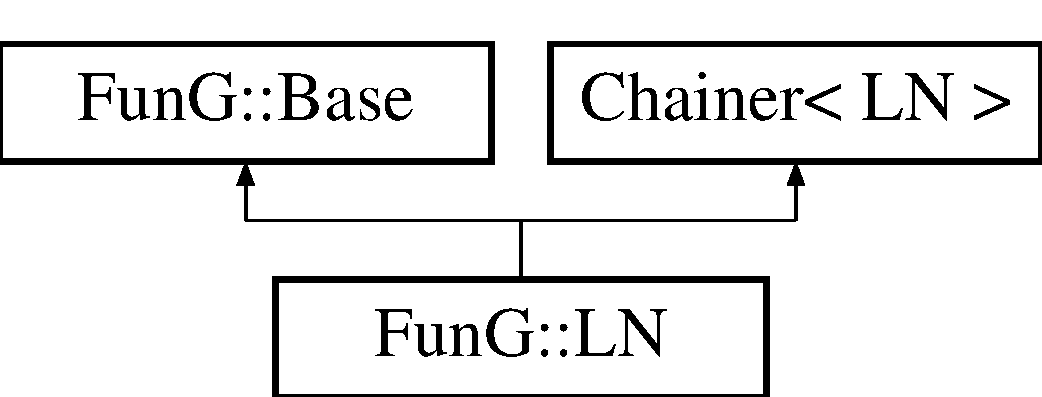
\includegraphics[height=2.000000cm]{structFunG_1_1LN}
\end{center}
\end{figure}
\subsection*{Public Member Functions}
\begin{DoxyCompactItemize}
\item 
\hyperlink{structFunG_1_1LN_a4ce3d29669f550f6033da3e52fdac392}{L\-N} (double x=1.)
\begin{DoxyCompactList}\small\item\em Constructor. \end{DoxyCompactList}\item 
\hypertarget{structFunG_1_1LN_aa0d58d6017b3c5bda5bef8f7936c6793}{void \hyperlink{structFunG_1_1LN_aa0d58d6017b3c5bda5bef8f7936c6793}{update} (double x)}\label{structFunG_1_1LN_aa0d58d6017b3c5bda5bef8f7936c6793}

\begin{DoxyCompactList}\small\item\em Reset point of evaluation. \end{DoxyCompactList}\item 
\hypertarget{structFunG_1_1LN_ad3c5a2c592af1edaac73584e3f238485}{double \hyperlink{structFunG_1_1LN_ad3c5a2c592af1edaac73584e3f238485}{d0} () const noexcept}\label{structFunG_1_1LN_ad3c5a2c592af1edaac73584e3f238485}

\begin{DoxyCompactList}\small\item\em Function value. \end{DoxyCompactList}\item 
\hypertarget{structFunG_1_1LN_a421d96cef93acfc5b766e2c00ffeb9cf}{{\footnotesize template$<$int  = -\/1$>$ }\\double \hyperlink{structFunG_1_1LN_a421d96cef93acfc5b766e2c00ffeb9cf}{d1} (double dx=1.) const }\label{structFunG_1_1LN_a421d96cef93acfc5b766e2c00ffeb9cf}

\begin{DoxyCompactList}\small\item\em First (directional) derivative. \end{DoxyCompactList}\item 
\hypertarget{structFunG_1_1LN_af7eb9ff5760deccc5a35fff41c803ab5}{{\footnotesize template$<$int  = -\/1, int  = -\/1$>$ }\\double \hyperlink{structFunG_1_1LN_af7eb9ff5760deccc5a35fff41c803ab5}{d2} (double dx=1., double dy=1.) const }\label{structFunG_1_1LN_af7eb9ff5760deccc5a35fff41c803ab5}

\begin{DoxyCompactList}\small\item\em Second (directional) derivative. \end{DoxyCompactList}\item 
\hypertarget{structFunG_1_1LN_a9e5b4095590b12b6cf14654bd47e3950}{{\footnotesize template$<$int  = -\/1, int  = -\/1, int  = -\/1$>$ }\\double \hyperlink{structFunG_1_1LN_a9e5b4095590b12b6cf14654bd47e3950}{d3} (double dx=1., double dy=1., double dz=1.) const }\label{structFunG_1_1LN_a9e5b4095590b12b6cf14654bd47e3950}

\begin{DoxyCompactList}\small\item\em Third (directional) derivative. \end{DoxyCompactList}\end{DoxyCompactItemize}


\subsection{Detailed Description}
Natural logarithm including first three derivatives. 

For scalar functions directional derivatives are less interesting. Incorporating this function as building block for more complex functions requires directional derivatives. These occur during applications of the chain rule. 

\subsection{Constructor \& Destructor Documentation}
\hypertarget{structFunG_1_1LN_a4ce3d29669f550f6033da3e52fdac392}{\index{Fun\-G\-::\-L\-N@{Fun\-G\-::\-L\-N}!L\-N@{L\-N}}
\index{L\-N@{L\-N}!FunG::LN@{Fun\-G\-::\-L\-N}}
\subsubsection[{L\-N}]{\setlength{\rightskip}{0pt plus 5cm}Fun\-G\-::\-L\-N\-::\-L\-N (
\begin{DoxyParamCaption}
\item[{double}]{x = {\ttfamily 1.}}
\end{DoxyParamCaption}
)\hspace{0.3cm}{\ttfamily [inline]}, {\ttfamily [explicit]}}}\label{structFunG_1_1LN_a4ce3d29669f550f6033da3e52fdac392}


Constructor. 


\begin{DoxyParams}{Parameters}
{\em x} & point of evaluation. \\
\hline
\end{DoxyParams}


The documentation for this struct was generated from the following file\-:\begin{DoxyCompactItemize}
\item 
fung/cmath/log.\-hh\end{DoxyCompactItemize}

\hypertarget{structFunG_1_1texify_1_1LN}{\section{Fun\-G\-:\-:texify\-:\-:L\-N Struct Reference}
\label{structFunG_1_1texify_1_1LN}\index{Fun\-G\-::texify\-::\-L\-N@{Fun\-G\-::texify\-::\-L\-N}}
}


{\ttfamily \#include $<$log.\-hh$>$}

Inheritance diagram for Fun\-G\-:\-:texify\-:\-:L\-N\-:\begin{figure}[H]
\begin{center}
\leavevmode
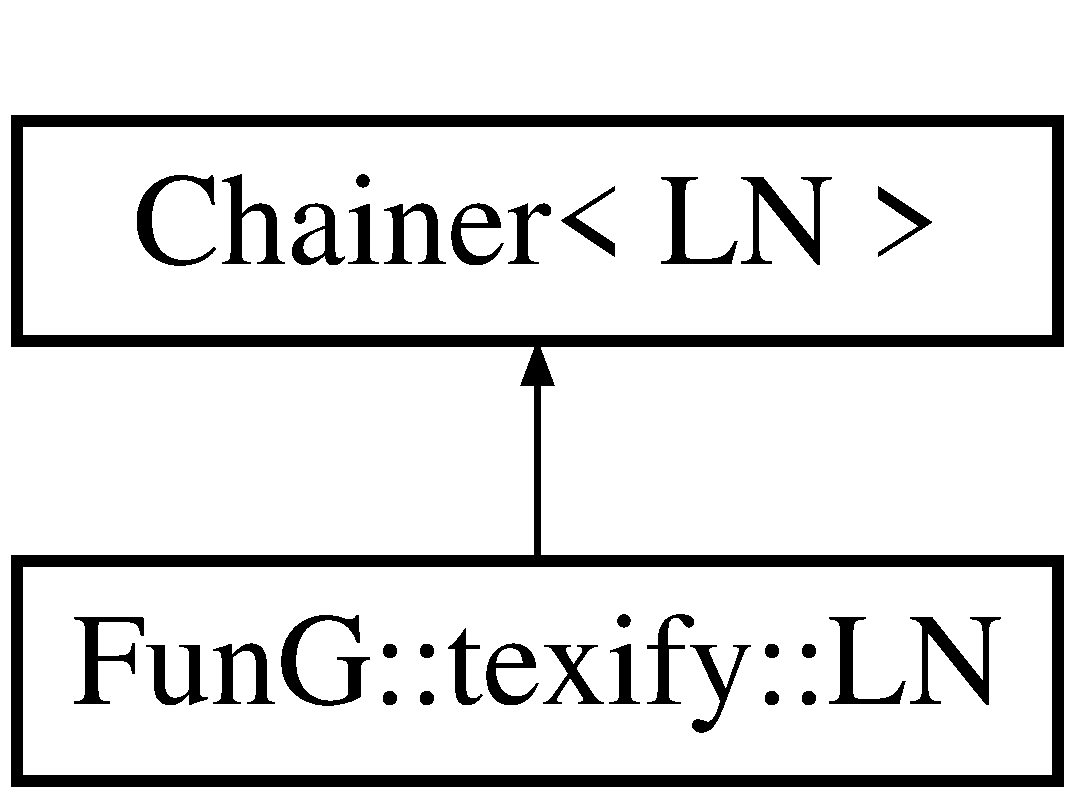
\includegraphics[height=2.000000cm]{structFunG_1_1texify_1_1LN}
\end{center}
\end{figure}
\subsection*{Public Member Functions}
\begin{DoxyCompactItemize}
\item 
\hyperlink{structFunG_1_1texify_1_1LN_ac03ec5ea34f9512638351cc57481bb41}{L\-N} (const std\-::string \&x=\char`\"{}x\char`\"{})
\begin{DoxyCompactList}\small\item\em Constructor. \end{DoxyCompactList}\item 
void \hyperlink{structFunG_1_1texify_1_1LN_a4e6d31d55ae11d0373c2e4c928988b7e}{update} (const std\-::string \&x)
\begin{DoxyCompactList}\small\item\em Set point of evaluation. \end{DoxyCompactList}\item 
std\-::string \hyperlink{structFunG_1_1texify_1_1LN_a383f0c9c02830607f55b3286b2a9088e}{d0} () const noexcept
\begin{DoxyCompactList}\small\item\em Function value. \end{DoxyCompactList}\item 
std\-::string \hyperlink{structFunG_1_1texify_1_1LN_a3b19e2918fec4eaa9cff95010c633235}{d1} (const std\-::string \&dx=\char`\"{}\char`\"{}) const 
\begin{DoxyCompactList}\small\item\em First (directional) derivative. \end{DoxyCompactList}\item 
std\-::string \hyperlink{structFunG_1_1texify_1_1LN_a68f8c6337531c83d107b2bf4b3acb89e}{d2} (const std\-::string \&dx=\char`\"{}\char`\"{}, const std\-::string \&dy=\char`\"{}\char`\"{}) const 
\begin{DoxyCompactList}\small\item\em Second (directional) derivative. \end{DoxyCompactList}\item 
std\-::string \hyperlink{structFunG_1_1texify_1_1LN_a571f67f455cba96ab397162c1e8ad4b1}{d3} (const std\-::string \&dx=\char`\"{}\char`\"{}, const std\-::string \&dy=\char`\"{}\char`\"{}, const std\-::string \&dz=\char`\"{}\char`\"{}) const 
\begin{DoxyCompactList}\small\item\em Third (directional) derivative. \end{DoxyCompactList}\end{DoxyCompactItemize}


\subsection{Constructor \& Destructor Documentation}
\hypertarget{structFunG_1_1texify_1_1LN_ac03ec5ea34f9512638351cc57481bb41}{\index{Fun\-G\-::texify\-::\-L\-N@{Fun\-G\-::texify\-::\-L\-N}!L\-N@{L\-N}}
\index{L\-N@{L\-N}!FunG::texify::LN@{Fun\-G\-::texify\-::\-L\-N}}
\subsubsection[{L\-N}]{\setlength{\rightskip}{0pt plus 5cm}Fun\-G\-::texify\-::\-L\-N\-::\-L\-N (
\begin{DoxyParamCaption}
\item[{const std\-::string \&}]{x = {\ttfamily \char`\"{}x\char`\"{}}}
\end{DoxyParamCaption}
)\hspace{0.3cm}{\ttfamily [inline]}, {\ttfamily [explicit]}}}\label{structFunG_1_1texify_1_1LN_ac03ec5ea34f9512638351cc57481bb41}


Constructor. 


\begin{DoxyParams}{Parameters}
{\em x} & point of evaluation \\
\hline
\end{DoxyParams}


\subsection{Member Function Documentation}
\hypertarget{structFunG_1_1texify_1_1LN_a383f0c9c02830607f55b3286b2a9088e}{\index{Fun\-G\-::texify\-::\-L\-N@{Fun\-G\-::texify\-::\-L\-N}!d0@{d0}}
\index{d0@{d0}!FunG::texify::LN@{Fun\-G\-::texify\-::\-L\-N}}
\subsubsection[{d0}]{\setlength{\rightskip}{0pt plus 5cm}std\-::string Fun\-G\-::texify\-::\-L\-N\-::d0 (
\begin{DoxyParamCaption}
{}
\end{DoxyParamCaption}
) const\hspace{0.3cm}{\ttfamily [inline]}, {\ttfamily [noexcept]}}}\label{structFunG_1_1texify_1_1LN_a383f0c9c02830607f55b3286b2a9088e}


Function value. 

\hypertarget{structFunG_1_1texify_1_1LN_a3b19e2918fec4eaa9cff95010c633235}{\index{Fun\-G\-::texify\-::\-L\-N@{Fun\-G\-::texify\-::\-L\-N}!d1@{d1}}
\index{d1@{d1}!FunG::texify::LN@{Fun\-G\-::texify\-::\-L\-N}}
\subsubsection[{d1}]{\setlength{\rightskip}{0pt plus 5cm}std\-::string Fun\-G\-::texify\-::\-L\-N\-::d1 (
\begin{DoxyParamCaption}
\item[{const std\-::string \&}]{dx = {\ttfamily \char`\"{}\char`\"{}}}
\end{DoxyParamCaption}
) const\hspace{0.3cm}{\ttfamily [inline]}}}\label{structFunG_1_1texify_1_1LN_a3b19e2918fec4eaa9cff95010c633235}


First (directional) derivative. 

\hypertarget{structFunG_1_1texify_1_1LN_a68f8c6337531c83d107b2bf4b3acb89e}{\index{Fun\-G\-::texify\-::\-L\-N@{Fun\-G\-::texify\-::\-L\-N}!d2@{d2}}
\index{d2@{d2}!FunG::texify::LN@{Fun\-G\-::texify\-::\-L\-N}}
\subsubsection[{d2}]{\setlength{\rightskip}{0pt plus 5cm}std\-::string Fun\-G\-::texify\-::\-L\-N\-::d2 (
\begin{DoxyParamCaption}
\item[{const std\-::string \&}]{dx = {\ttfamily \char`\"{}\char`\"{}}, }
\item[{const std\-::string \&}]{dy = {\ttfamily \char`\"{}\char`\"{}}}
\end{DoxyParamCaption}
) const\hspace{0.3cm}{\ttfamily [inline]}}}\label{structFunG_1_1texify_1_1LN_a68f8c6337531c83d107b2bf4b3acb89e}


Second (directional) derivative. 

\hypertarget{structFunG_1_1texify_1_1LN_a571f67f455cba96ab397162c1e8ad4b1}{\index{Fun\-G\-::texify\-::\-L\-N@{Fun\-G\-::texify\-::\-L\-N}!d3@{d3}}
\index{d3@{d3}!FunG::texify::LN@{Fun\-G\-::texify\-::\-L\-N}}
\subsubsection[{d3}]{\setlength{\rightskip}{0pt plus 5cm}std\-::string Fun\-G\-::texify\-::\-L\-N\-::d3 (
\begin{DoxyParamCaption}
\item[{const std\-::string \&}]{dx = {\ttfamily \char`\"{}\char`\"{}}, }
\item[{const std\-::string \&}]{dy = {\ttfamily \char`\"{}\char`\"{}}, }
\item[{const std\-::string \&}]{dz = {\ttfamily \char`\"{}\char`\"{}}}
\end{DoxyParamCaption}
) const\hspace{0.3cm}{\ttfamily [inline]}}}\label{structFunG_1_1texify_1_1LN_a571f67f455cba96ab397162c1e8ad4b1}


Third (directional) derivative. 

\hypertarget{structFunG_1_1texify_1_1LN_a4e6d31d55ae11d0373c2e4c928988b7e}{\index{Fun\-G\-::texify\-::\-L\-N@{Fun\-G\-::texify\-::\-L\-N}!update@{update}}
\index{update@{update}!FunG::texify::LN@{Fun\-G\-::texify\-::\-L\-N}}
\subsubsection[{update}]{\setlength{\rightskip}{0pt plus 5cm}void Fun\-G\-::texify\-::\-L\-N\-::update (
\begin{DoxyParamCaption}
\item[{const std\-::string \&}]{x}
\end{DoxyParamCaption}
)\hspace{0.3cm}{\ttfamily [inline]}}}\label{structFunG_1_1texify_1_1LN_a4e6d31d55ae11d0373c2e4c928988b7e}


Set point of evaluation. 



The documentation for this struct was generated from the following file\-:\begin{DoxyCompactItemize}
\item 
include/fung/texify/cmath/\hyperlink{texify_2cmath_2log_8hh}{log.\-hh}\end{DoxyCompactItemize}

\hypertarget{structFunG_1_1stringify_1_1Log10}{\section{Fun\-G\-:\-:stringify\-:\-:Log10 Struct Reference}
\label{structFunG_1_1stringify_1_1Log10}\index{Fun\-G\-::stringify\-::\-Log10@{Fun\-G\-::stringify\-::\-Log10}}
}


Common (base 10) logarithm including first three derivatives.  




{\ttfamily \#include $<$log.\-hh$>$}

Inheritance diagram for Fun\-G\-:\-:stringify\-:\-:Log10\-:\begin{figure}[H]
\begin{center}
\leavevmode
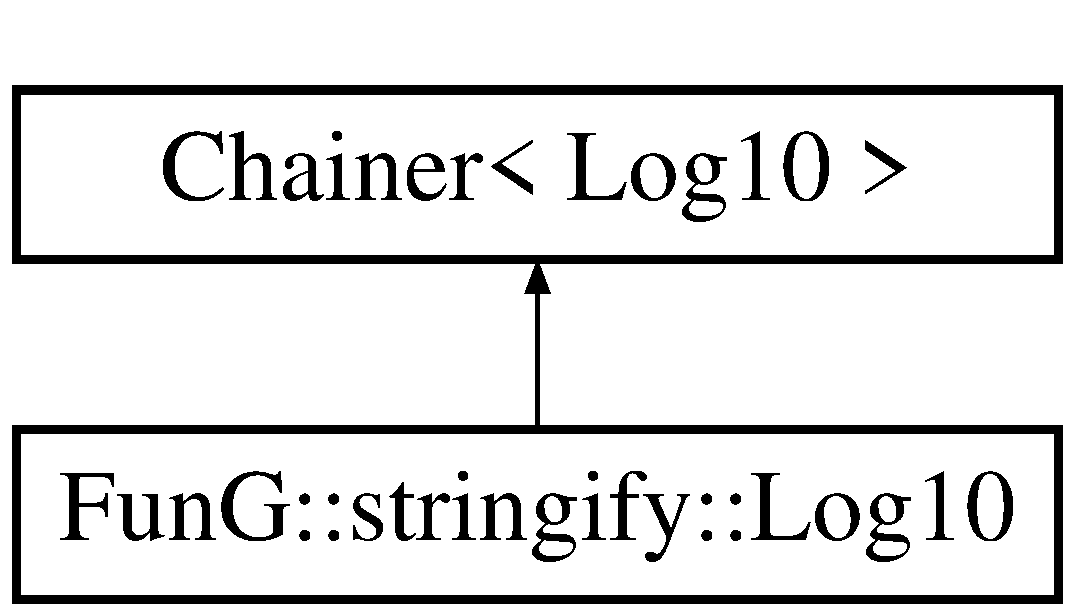
\includegraphics[height=2.000000cm]{structFunG_1_1stringify_1_1Log10}
\end{center}
\end{figure}
\subsection*{Public Member Functions}
\begin{DoxyCompactItemize}
\item 
\hyperlink{structFunG_1_1stringify_1_1Log10_ac9c116740e7f9eac972dd9d8c1bae4a2}{Log10} (const std\-::string \&x=\char`\"{}x\char`\"{})
\begin{DoxyCompactList}\small\item\em Constructor. \end{DoxyCompactList}\item 
void \hyperlink{structFunG_1_1stringify_1_1Log10_a891be13cee4444f379ccc39425f42981}{update} (const std\-::string \&x)
\begin{DoxyCompactList}\small\item\em Set point of evaluation. \end{DoxyCompactList}\item 
std\-::string \hyperlink{structFunG_1_1stringify_1_1Log10_ad72e5992fac1dc95c150bb42b1449cff}{d0} () const noexcept
\begin{DoxyCompactList}\small\item\em Function value. \end{DoxyCompactList}\item 
std\-::string \hyperlink{structFunG_1_1stringify_1_1Log10_a691846f87fafe5bbf9eb60d3503bdc4e}{d1} (const std\-::string \&dx=\char`\"{}\char`\"{}) const 
\begin{DoxyCompactList}\small\item\em First (directional) derivative. \end{DoxyCompactList}\item 
std\-::string \hyperlink{structFunG_1_1stringify_1_1Log10_a01163482ea8ad8dddffe3fcf1bb5bb9c}{d2} (const std\-::string \&dx=\char`\"{}\char`\"{}, const std\-::string \&dy=\char`\"{}\char`\"{}) const 
\begin{DoxyCompactList}\small\item\em Second (directional) derivative. \end{DoxyCompactList}\item 
std\-::string \hyperlink{structFunG_1_1stringify_1_1Log10_ab77f394476f8f761e5c3a76e8767f7bb}{d3} (const std\-::string \&dx=\char`\"{}\char`\"{}, const std\-::string \&dy=\char`\"{}\char`\"{}, const std\-::string \&dz=\char`\"{}\char`\"{}) const 
\begin{DoxyCompactList}\small\item\em Third (directional) derivative. \end{DoxyCompactList}\end{DoxyCompactItemize}


\subsection{Detailed Description}
Common (base 10) logarithm including first three derivatives. 

For scalar functions directional derivatives are less interesting. Incorporating this function as building block for more complex functions requires directional derivatives. These occur during applications of the chain rule. 

\subsection{Constructor \& Destructor Documentation}
\hypertarget{structFunG_1_1stringify_1_1Log10_ac9c116740e7f9eac972dd9d8c1bae4a2}{\index{Fun\-G\-::stringify\-::\-Log10@{Fun\-G\-::stringify\-::\-Log10}!Log10@{Log10}}
\index{Log10@{Log10}!FunG::stringify::Log10@{Fun\-G\-::stringify\-::\-Log10}}
\subsubsection[{Log10}]{\setlength{\rightskip}{0pt plus 5cm}Fun\-G\-::stringify\-::\-Log10\-::\-Log10 (
\begin{DoxyParamCaption}
\item[{const std\-::string \&}]{x = {\ttfamily \char`\"{}x\char`\"{}}}
\end{DoxyParamCaption}
)\hspace{0.3cm}{\ttfamily [inline]}, {\ttfamily [explicit]}}}\label{structFunG_1_1stringify_1_1Log10_ac9c116740e7f9eac972dd9d8c1bae4a2}


Constructor. 


\begin{DoxyParams}{Parameters}
{\em x} & point of evaluation \\
\hline
\end{DoxyParams}


\subsection{Member Function Documentation}
\hypertarget{structFunG_1_1stringify_1_1Log10_ad72e5992fac1dc95c150bb42b1449cff}{\index{Fun\-G\-::stringify\-::\-Log10@{Fun\-G\-::stringify\-::\-Log10}!d0@{d0}}
\index{d0@{d0}!FunG::stringify::Log10@{Fun\-G\-::stringify\-::\-Log10}}
\subsubsection[{d0}]{\setlength{\rightskip}{0pt plus 5cm}std\-::string Fun\-G\-::stringify\-::\-Log10\-::d0 (
\begin{DoxyParamCaption}
{}
\end{DoxyParamCaption}
) const\hspace{0.3cm}{\ttfamily [inline]}, {\ttfamily [noexcept]}}}\label{structFunG_1_1stringify_1_1Log10_ad72e5992fac1dc95c150bb42b1449cff}


Function value. 

\hypertarget{structFunG_1_1stringify_1_1Log10_a691846f87fafe5bbf9eb60d3503bdc4e}{\index{Fun\-G\-::stringify\-::\-Log10@{Fun\-G\-::stringify\-::\-Log10}!d1@{d1}}
\index{d1@{d1}!FunG::stringify::Log10@{Fun\-G\-::stringify\-::\-Log10}}
\subsubsection[{d1}]{\setlength{\rightskip}{0pt plus 5cm}std\-::string Fun\-G\-::stringify\-::\-Log10\-::d1 (
\begin{DoxyParamCaption}
\item[{const std\-::string \&}]{dx = {\ttfamily \char`\"{}\char`\"{}}}
\end{DoxyParamCaption}
) const\hspace{0.3cm}{\ttfamily [inline]}}}\label{structFunG_1_1stringify_1_1Log10_a691846f87fafe5bbf9eb60d3503bdc4e}


First (directional) derivative. 

\hypertarget{structFunG_1_1stringify_1_1Log10_a01163482ea8ad8dddffe3fcf1bb5bb9c}{\index{Fun\-G\-::stringify\-::\-Log10@{Fun\-G\-::stringify\-::\-Log10}!d2@{d2}}
\index{d2@{d2}!FunG::stringify::Log10@{Fun\-G\-::stringify\-::\-Log10}}
\subsubsection[{d2}]{\setlength{\rightskip}{0pt plus 5cm}std\-::string Fun\-G\-::stringify\-::\-Log10\-::d2 (
\begin{DoxyParamCaption}
\item[{const std\-::string \&}]{dx = {\ttfamily \char`\"{}\char`\"{}}, }
\item[{const std\-::string \&}]{dy = {\ttfamily \char`\"{}\char`\"{}}}
\end{DoxyParamCaption}
) const\hspace{0.3cm}{\ttfamily [inline]}}}\label{structFunG_1_1stringify_1_1Log10_a01163482ea8ad8dddffe3fcf1bb5bb9c}


Second (directional) derivative. 

\hypertarget{structFunG_1_1stringify_1_1Log10_ab77f394476f8f761e5c3a76e8767f7bb}{\index{Fun\-G\-::stringify\-::\-Log10@{Fun\-G\-::stringify\-::\-Log10}!d3@{d3}}
\index{d3@{d3}!FunG::stringify::Log10@{Fun\-G\-::stringify\-::\-Log10}}
\subsubsection[{d3}]{\setlength{\rightskip}{0pt plus 5cm}std\-::string Fun\-G\-::stringify\-::\-Log10\-::d3 (
\begin{DoxyParamCaption}
\item[{const std\-::string \&}]{dx = {\ttfamily \char`\"{}\char`\"{}}, }
\item[{const std\-::string \&}]{dy = {\ttfamily \char`\"{}\char`\"{}}, }
\item[{const std\-::string \&}]{dz = {\ttfamily \char`\"{}\char`\"{}}}
\end{DoxyParamCaption}
) const\hspace{0.3cm}{\ttfamily [inline]}}}\label{structFunG_1_1stringify_1_1Log10_ab77f394476f8f761e5c3a76e8767f7bb}


Third (directional) derivative. 

\hypertarget{structFunG_1_1stringify_1_1Log10_a891be13cee4444f379ccc39425f42981}{\index{Fun\-G\-::stringify\-::\-Log10@{Fun\-G\-::stringify\-::\-Log10}!update@{update}}
\index{update@{update}!FunG::stringify::Log10@{Fun\-G\-::stringify\-::\-Log10}}
\subsubsection[{update}]{\setlength{\rightskip}{0pt plus 5cm}void Fun\-G\-::stringify\-::\-Log10\-::update (
\begin{DoxyParamCaption}
\item[{const std\-::string \&}]{x}
\end{DoxyParamCaption}
)\hspace{0.3cm}{\ttfamily [inline]}}}\label{structFunG_1_1stringify_1_1Log10_a891be13cee4444f379ccc39425f42981}


Set point of evaluation. 



The documentation for this struct was generated from the following file\-:\begin{DoxyCompactItemize}
\item 
include/fung/stringify/cmath/\hyperlink{stringify_2cmath_2log_8hh}{log.\-hh}\end{DoxyCompactItemize}

\hypertarget{structFunG_1_1Log10}{\section{Fun\-G\-:\-:Log10 Struct Reference}
\label{structFunG_1_1Log10}\index{Fun\-G\-::\-Log10@{Fun\-G\-::\-Log10}}
}


Common (base 10) logarithm including first three derivatives.  




{\ttfamily \#include $<$log.\-hh$>$}

Inheritance diagram for Fun\-G\-:\-:Log10\-:\begin{figure}[H]
\begin{center}
\leavevmode
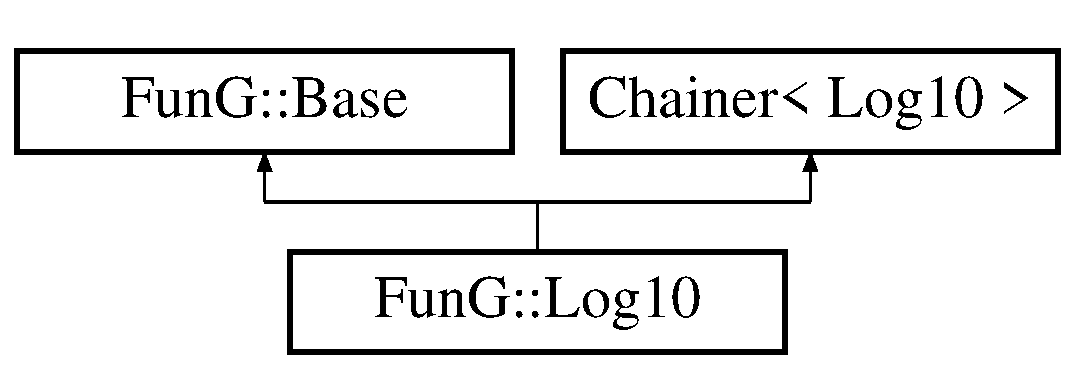
\includegraphics[height=2.000000cm]{structFunG_1_1Log10}
\end{center}
\end{figure}
\subsection*{Public Member Functions}
\begin{DoxyCompactItemize}
\item 
\hyperlink{structFunG_1_1Log10_acfc491f166bfb75b593864849f33fbb0}{Log10} (double x=1.)
\begin{DoxyCompactList}\small\item\em Constructor. \end{DoxyCompactList}\item 
void \hyperlink{structFunG_1_1Log10_a232acaf336d555a2d4b9eefb5dee4272}{update} (double x)
\begin{DoxyCompactList}\small\item\em Set point of evaluation. \end{DoxyCompactList}\item 
double \hyperlink{structFunG_1_1Log10_a0046c146e0a7111ec65acf8ee13c7d85}{d0} () const noexcept
\begin{DoxyCompactList}\small\item\em Function value. \end{DoxyCompactList}\item 
double \hyperlink{structFunG_1_1Log10_aa58c6a61851745d626ada5485331f51c}{d1} (double dx=1.) const 
\begin{DoxyCompactList}\small\item\em First (directional) derivative. \end{DoxyCompactList}\item 
double \hyperlink{structFunG_1_1Log10_a54c3c5131cf317a2188a07a5f56e87c1}{d2} (double dx=1., double dy=1.) const 
\begin{DoxyCompactList}\small\item\em Second (directional) derivative. \end{DoxyCompactList}\item 
double \hyperlink{structFunG_1_1Log10_a385b674f76566344a0188bf8f213b5ec}{d3} (double dx=1., double dy=1., double dz=1.) const 
\begin{DoxyCompactList}\small\item\em Third (directional) derivative. \end{DoxyCompactList}\end{DoxyCompactItemize}


\subsection{Detailed Description}
Common (base 10) logarithm including first three derivatives. 

For scalar functions directional derivatives are less interesting. Incorporating this function as building block for more complex functions requires directional derivatives. These occur during applications of the chain rule. 

\subsection{Constructor \& Destructor Documentation}
\hypertarget{structFunG_1_1Log10_acfc491f166bfb75b593864849f33fbb0}{\index{Fun\-G\-::\-Log10@{Fun\-G\-::\-Log10}!Log10@{Log10}}
\index{Log10@{Log10}!FunG::Log10@{Fun\-G\-::\-Log10}}
\subsubsection[{Log10}]{\setlength{\rightskip}{0pt plus 5cm}Fun\-G\-::\-Log10\-::\-Log10 (
\begin{DoxyParamCaption}
\item[{double}]{x = {\ttfamily 1.}}
\end{DoxyParamCaption}
)\hspace{0.3cm}{\ttfamily [inline]}, {\ttfamily [explicit]}}}\label{structFunG_1_1Log10_acfc491f166bfb75b593864849f33fbb0}


Constructor. 


\begin{DoxyParams}{Parameters}
{\em x} & point of evaluation \\
\hline
\end{DoxyParams}


\subsection{Member Function Documentation}
\hypertarget{structFunG_1_1Log10_a0046c146e0a7111ec65acf8ee13c7d85}{\index{Fun\-G\-::\-Log10@{Fun\-G\-::\-Log10}!d0@{d0}}
\index{d0@{d0}!FunG::Log10@{Fun\-G\-::\-Log10}}
\subsubsection[{d0}]{\setlength{\rightskip}{0pt plus 5cm}double Fun\-G\-::\-Log10\-::d0 (
\begin{DoxyParamCaption}
{}
\end{DoxyParamCaption}
) const\hspace{0.3cm}{\ttfamily [inline]}, {\ttfamily [noexcept]}}}\label{structFunG_1_1Log10_a0046c146e0a7111ec65acf8ee13c7d85}


Function value. 

\hypertarget{structFunG_1_1Log10_aa58c6a61851745d626ada5485331f51c}{\index{Fun\-G\-::\-Log10@{Fun\-G\-::\-Log10}!d1@{d1}}
\index{d1@{d1}!FunG::Log10@{Fun\-G\-::\-Log10}}
\subsubsection[{d1}]{\setlength{\rightskip}{0pt plus 5cm}double Fun\-G\-::\-Log10\-::d1 (
\begin{DoxyParamCaption}
\item[{double}]{dx = {\ttfamily 1.}}
\end{DoxyParamCaption}
) const\hspace{0.3cm}{\ttfamily [inline]}}}\label{structFunG_1_1Log10_aa58c6a61851745d626ada5485331f51c}


First (directional) derivative. 

\hypertarget{structFunG_1_1Log10_a54c3c5131cf317a2188a07a5f56e87c1}{\index{Fun\-G\-::\-Log10@{Fun\-G\-::\-Log10}!d2@{d2}}
\index{d2@{d2}!FunG::Log10@{Fun\-G\-::\-Log10}}
\subsubsection[{d2}]{\setlength{\rightskip}{0pt plus 5cm}double Fun\-G\-::\-Log10\-::d2 (
\begin{DoxyParamCaption}
\item[{double}]{dx = {\ttfamily 1.}, }
\item[{double}]{dy = {\ttfamily 1.}}
\end{DoxyParamCaption}
) const\hspace{0.3cm}{\ttfamily [inline]}}}\label{structFunG_1_1Log10_a54c3c5131cf317a2188a07a5f56e87c1}


Second (directional) derivative. 

\hypertarget{structFunG_1_1Log10_a385b674f76566344a0188bf8f213b5ec}{\index{Fun\-G\-::\-Log10@{Fun\-G\-::\-Log10}!d3@{d3}}
\index{d3@{d3}!FunG::Log10@{Fun\-G\-::\-Log10}}
\subsubsection[{d3}]{\setlength{\rightskip}{0pt plus 5cm}double Fun\-G\-::\-Log10\-::d3 (
\begin{DoxyParamCaption}
\item[{double}]{dx = {\ttfamily 1.}, }
\item[{double}]{dy = {\ttfamily 1.}, }
\item[{double}]{dz = {\ttfamily 1.}}
\end{DoxyParamCaption}
) const\hspace{0.3cm}{\ttfamily [inline]}}}\label{structFunG_1_1Log10_a385b674f76566344a0188bf8f213b5ec}


Third (directional) derivative. 

\hypertarget{structFunG_1_1Log10_a232acaf336d555a2d4b9eefb5dee4272}{\index{Fun\-G\-::\-Log10@{Fun\-G\-::\-Log10}!update@{update}}
\index{update@{update}!FunG::Log10@{Fun\-G\-::\-Log10}}
\subsubsection[{update}]{\setlength{\rightskip}{0pt plus 5cm}void Fun\-G\-::\-Log10\-::update (
\begin{DoxyParamCaption}
\item[{double}]{x}
\end{DoxyParamCaption}
)\hspace{0.3cm}{\ttfamily [inline]}}}\label{structFunG_1_1Log10_a232acaf336d555a2d4b9eefb5dee4272}


Set point of evaluation. 



The documentation for this struct was generated from the following file\-:\begin{DoxyCompactItemize}
\item 
include/fung/cmath/\hyperlink{log_8hh}{log.\-hh}\end{DoxyCompactItemize}

\hypertarget{structFunG_1_1texify_1_1Log10}{\section{Fun\-G\-:\-:texify\-:\-:Log10 Struct Reference}
\label{structFunG_1_1texify_1_1Log10}\index{Fun\-G\-::texify\-::\-Log10@{Fun\-G\-::texify\-::\-Log10}}
}


Common (base 10) logarithm including first three derivatives.  




{\ttfamily \#include $<$log.\-hh$>$}

Inheritance diagram for Fun\-G\-:\-:texify\-:\-:Log10\-:\begin{figure}[H]
\begin{center}
\leavevmode
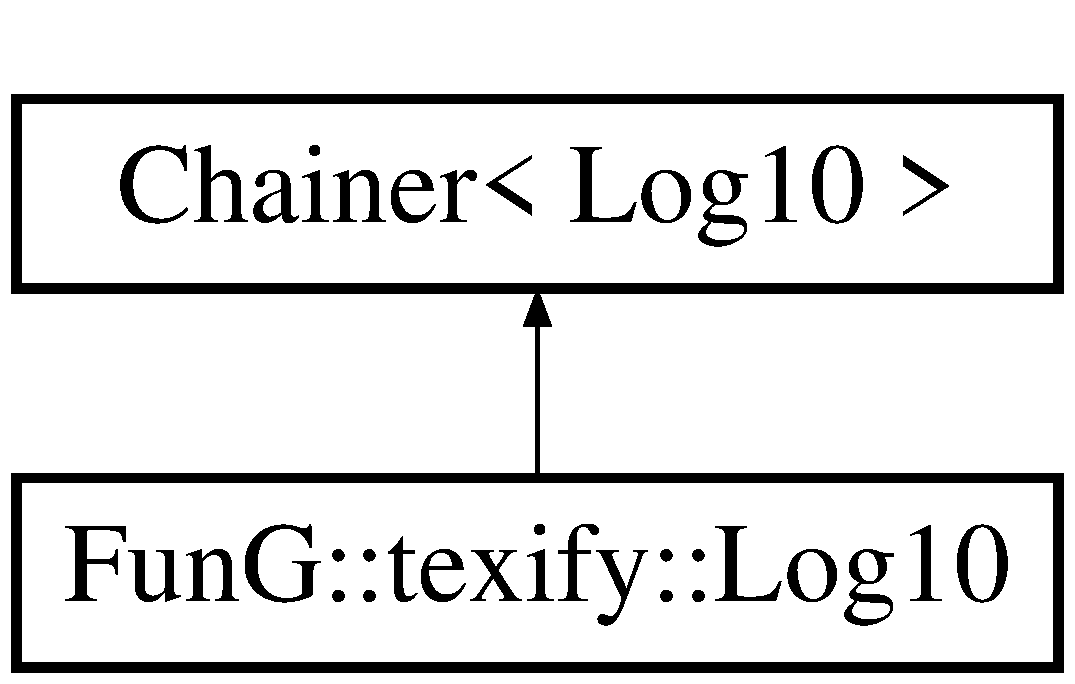
\includegraphics[height=2.000000cm]{structFunG_1_1texify_1_1Log10}
\end{center}
\end{figure}
\subsection*{Public Member Functions}
\begin{DoxyCompactItemize}
\item 
\hyperlink{structFunG_1_1texify_1_1Log10_ae612e34de03b93d577891342f1d537bf}{Log10} (const std\-::string \&x=\char`\"{}x\char`\"{})
\begin{DoxyCompactList}\small\item\em Constructor. \end{DoxyCompactList}\item 
void \hyperlink{structFunG_1_1texify_1_1Log10_a4a3c299d7e3c1b9ac3df21a44a06366a}{update} (const std\-::string \&x)
\begin{DoxyCompactList}\small\item\em Set point of evaluation. \end{DoxyCompactList}\item 
std\-::string \hyperlink{structFunG_1_1texify_1_1Log10_a0384f9355c5ef0cae3fc9923d3559795}{d0} () const noexcept
\begin{DoxyCompactList}\small\item\em Function value. \end{DoxyCompactList}\item 
std\-::string \hyperlink{structFunG_1_1texify_1_1Log10_ab9dadd055804d4b1f65962078b5d20a7}{d1} (const std\-::string \&dx=\char`\"{}\char`\"{}) const 
\begin{DoxyCompactList}\small\item\em First (directional) derivative. \end{DoxyCompactList}\item 
std\-::string \hyperlink{structFunG_1_1texify_1_1Log10_aac6d28a6d124725bebaad3e39e41bf84}{d2} (const std\-::string \&dx=\char`\"{}\char`\"{}, const std\-::string \&dy=\char`\"{}\char`\"{}) const 
\begin{DoxyCompactList}\small\item\em Second (directional) derivative. \end{DoxyCompactList}\item 
std\-::string \hyperlink{structFunG_1_1texify_1_1Log10_a1e7fd7a64eee30baa685d3450799e75a}{d3} (const std\-::string \&dx=\char`\"{}\char`\"{}, const std\-::string \&dy=\char`\"{}\char`\"{}, const std\-::string \&dz=\char`\"{}\char`\"{}) const 
\begin{DoxyCompactList}\small\item\em Third (directional) derivative. \end{DoxyCompactList}\end{DoxyCompactItemize}


\subsection{Detailed Description}
Common (base 10) logarithm including first three derivatives. 

For scalar functions directional derivatives are less interesting. Incorporating this function as building block for more complex functions requires directional derivatives. These occur during applications of the chain rule. 

\subsection{Constructor \& Destructor Documentation}
\hypertarget{structFunG_1_1texify_1_1Log10_ae612e34de03b93d577891342f1d537bf}{\index{Fun\-G\-::texify\-::\-Log10@{Fun\-G\-::texify\-::\-Log10}!Log10@{Log10}}
\index{Log10@{Log10}!FunG::texify::Log10@{Fun\-G\-::texify\-::\-Log10}}
\subsubsection[{Log10}]{\setlength{\rightskip}{0pt plus 5cm}Fun\-G\-::texify\-::\-Log10\-::\-Log10 (
\begin{DoxyParamCaption}
\item[{const std\-::string \&}]{x = {\ttfamily \char`\"{}x\char`\"{}}}
\end{DoxyParamCaption}
)\hspace{0.3cm}{\ttfamily [inline]}, {\ttfamily [explicit]}}}\label{structFunG_1_1texify_1_1Log10_ae612e34de03b93d577891342f1d537bf}


Constructor. 


\begin{DoxyParams}{Parameters}
{\em x} & point of evaluation \\
\hline
\end{DoxyParams}


\subsection{Member Function Documentation}
\hypertarget{structFunG_1_1texify_1_1Log10_a0384f9355c5ef0cae3fc9923d3559795}{\index{Fun\-G\-::texify\-::\-Log10@{Fun\-G\-::texify\-::\-Log10}!d0@{d0}}
\index{d0@{d0}!FunG::texify::Log10@{Fun\-G\-::texify\-::\-Log10}}
\subsubsection[{d0}]{\setlength{\rightskip}{0pt plus 5cm}std\-::string Fun\-G\-::texify\-::\-Log10\-::d0 (
\begin{DoxyParamCaption}
{}
\end{DoxyParamCaption}
) const\hspace{0.3cm}{\ttfamily [inline]}, {\ttfamily [noexcept]}}}\label{structFunG_1_1texify_1_1Log10_a0384f9355c5ef0cae3fc9923d3559795}


Function value. 

\hypertarget{structFunG_1_1texify_1_1Log10_ab9dadd055804d4b1f65962078b5d20a7}{\index{Fun\-G\-::texify\-::\-Log10@{Fun\-G\-::texify\-::\-Log10}!d1@{d1}}
\index{d1@{d1}!FunG::texify::Log10@{Fun\-G\-::texify\-::\-Log10}}
\subsubsection[{d1}]{\setlength{\rightskip}{0pt plus 5cm}std\-::string Fun\-G\-::texify\-::\-Log10\-::d1 (
\begin{DoxyParamCaption}
\item[{const std\-::string \&}]{dx = {\ttfamily \char`\"{}\char`\"{}}}
\end{DoxyParamCaption}
) const\hspace{0.3cm}{\ttfamily [inline]}}}\label{structFunG_1_1texify_1_1Log10_ab9dadd055804d4b1f65962078b5d20a7}


First (directional) derivative. 

\hypertarget{structFunG_1_1texify_1_1Log10_aac6d28a6d124725bebaad3e39e41bf84}{\index{Fun\-G\-::texify\-::\-Log10@{Fun\-G\-::texify\-::\-Log10}!d2@{d2}}
\index{d2@{d2}!FunG::texify::Log10@{Fun\-G\-::texify\-::\-Log10}}
\subsubsection[{d2}]{\setlength{\rightskip}{0pt plus 5cm}std\-::string Fun\-G\-::texify\-::\-Log10\-::d2 (
\begin{DoxyParamCaption}
\item[{const std\-::string \&}]{dx = {\ttfamily \char`\"{}\char`\"{}}, }
\item[{const std\-::string \&}]{dy = {\ttfamily \char`\"{}\char`\"{}}}
\end{DoxyParamCaption}
) const\hspace{0.3cm}{\ttfamily [inline]}}}\label{structFunG_1_1texify_1_1Log10_aac6d28a6d124725bebaad3e39e41bf84}


Second (directional) derivative. 

\hypertarget{structFunG_1_1texify_1_1Log10_a1e7fd7a64eee30baa685d3450799e75a}{\index{Fun\-G\-::texify\-::\-Log10@{Fun\-G\-::texify\-::\-Log10}!d3@{d3}}
\index{d3@{d3}!FunG::texify::Log10@{Fun\-G\-::texify\-::\-Log10}}
\subsubsection[{d3}]{\setlength{\rightskip}{0pt plus 5cm}std\-::string Fun\-G\-::texify\-::\-Log10\-::d3 (
\begin{DoxyParamCaption}
\item[{const std\-::string \&}]{dx = {\ttfamily \char`\"{}\char`\"{}}, }
\item[{const std\-::string \&}]{dy = {\ttfamily \char`\"{}\char`\"{}}, }
\item[{const std\-::string \&}]{dz = {\ttfamily \char`\"{}\char`\"{}}}
\end{DoxyParamCaption}
) const\hspace{0.3cm}{\ttfamily [inline]}}}\label{structFunG_1_1texify_1_1Log10_a1e7fd7a64eee30baa685d3450799e75a}


Third (directional) derivative. 

\hypertarget{structFunG_1_1texify_1_1Log10_a4a3c299d7e3c1b9ac3df21a44a06366a}{\index{Fun\-G\-::texify\-::\-Log10@{Fun\-G\-::texify\-::\-Log10}!update@{update}}
\index{update@{update}!FunG::texify::Log10@{Fun\-G\-::texify\-::\-Log10}}
\subsubsection[{update}]{\setlength{\rightskip}{0pt plus 5cm}void Fun\-G\-::texify\-::\-Log10\-::update (
\begin{DoxyParamCaption}
\item[{const std\-::string \&}]{x}
\end{DoxyParamCaption}
)\hspace{0.3cm}{\ttfamily [inline]}}}\label{structFunG_1_1texify_1_1Log10_a4a3c299d7e3c1b9ac3df21a44a06366a}


Set point of evaluation. 



The documentation for this struct was generated from the following file\-:\begin{DoxyCompactItemize}
\item 
include/fung/texify/cmath/\hyperlink{texify_2cmath_2log_8hh}{log.\-hh}\end{DoxyCompactItemize}

\hypertarget{structFunG_1_1Log2}{}\section{FunG\+:\+:Log2 Struct Reference}
\label{structFunG_1_1Log2}\index{Fun\+G\+::\+Log2@{Fun\+G\+::\+Log2}}


Base 2 logarithm including first three derivatives.  




{\ttfamily \#include $<$log.\+hh$>$}

Inheritance diagram for FunG\+:\+:Log2\+:\begin{figure}[H]
\begin{center}
\leavevmode
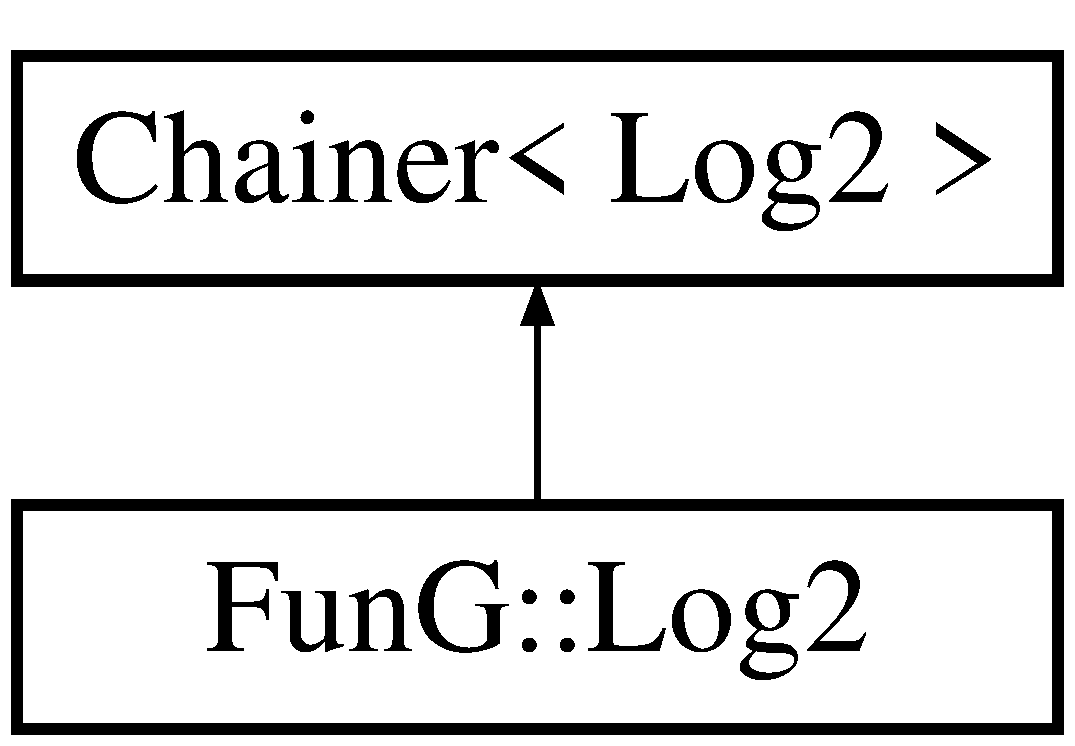
\includegraphics[height=2.000000cm]{structFunG_1_1Log2}
\end{center}
\end{figure}
\subsection*{Public Member Functions}
\begin{DoxyCompactItemize}
\item 
\hyperlink{structFunG_1_1Log2_ab3fe35bf3d976e51797bff7128d2f16b}{Log2} (double x=1.)
\begin{DoxyCompactList}\small\item\em Constructor. \end{DoxyCompactList}\item 
void \hyperlink{structFunG_1_1Log2_a2052168d207ca31e00620238c71b94f3}{update} (double x)
\begin{DoxyCompactList}\small\item\em Set point of evaluation. \end{DoxyCompactList}\item 
double \hyperlink{structFunG_1_1Log2_a11b6311bb395c3e77cdb874ec2eab240}{d0} () const noexcept
\begin{DoxyCompactList}\small\item\em Function value. \end{DoxyCompactList}\item 
double \hyperlink{structFunG_1_1Log2_ab8d1169c44c1940953c19e85e292a9b9}{d1} (double dx=1.) const 
\begin{DoxyCompactList}\small\item\em First (directional) derivative. \end{DoxyCompactList}\item 
double \hyperlink{structFunG_1_1Log2_aa90f4f3ccfca5cff8d6027a04fae1ea1}{d2} (double dx=1., double dy=1.) const 
\begin{DoxyCompactList}\small\item\em Second (directional) derivative. \end{DoxyCompactList}\item 
double \hyperlink{structFunG_1_1Log2_a9012b223a7cc98604bcb3acd756b3902}{d3} (double dx=1., double dy=1., double dz=1.) const 
\begin{DoxyCompactList}\small\item\em Third (directional) derivative. \end{DoxyCompactList}\end{DoxyCompactItemize}


\subsection{Detailed Description}
Base 2 logarithm including first three derivatives. 

For scalar functions directional derivatives are less interesting. Incorporating this function as building block for more complex functions requires directional derivatives. These occur during applications of the chain rule. 

\subsection{Constructor \& Destructor Documentation}
\index{Fun\+G\+::\+Log2@{Fun\+G\+::\+Log2}!Log2@{Log2}}
\index{Log2@{Log2}!Fun\+G\+::\+Log2@{Fun\+G\+::\+Log2}}
\subsubsection[{\texorpdfstring{Log2(double x=1.)}{Log2(double x=1.)}}]{\setlength{\rightskip}{0pt plus 5cm}Fun\+G\+::\+Log2\+::\+Log2 (
\begin{DoxyParamCaption}
\item[{double}]{x = {\ttfamily 1.}}
\end{DoxyParamCaption}
)\hspace{0.3cm}{\ttfamily [inline]}, {\ttfamily [explicit]}}\hypertarget{structFunG_1_1Log2_ab3fe35bf3d976e51797bff7128d2f16b}{}\label{structFunG_1_1Log2_ab3fe35bf3d976e51797bff7128d2f16b}


Constructor. 


\begin{DoxyParams}{Parameters}
{\em x} & point of evaluation \\
\hline
\end{DoxyParams}


\subsection{Member Function Documentation}
\index{Fun\+G\+::\+Log2@{Fun\+G\+::\+Log2}!d0@{d0}}
\index{d0@{d0}!Fun\+G\+::\+Log2@{Fun\+G\+::\+Log2}}
\subsubsection[{\texorpdfstring{d0() const noexcept}{d0() const noexcept}}]{\setlength{\rightskip}{0pt plus 5cm}double Fun\+G\+::\+Log2\+::d0 (
\begin{DoxyParamCaption}
{}
\end{DoxyParamCaption}
) const\hspace{0.3cm}{\ttfamily [inline]}, {\ttfamily [noexcept]}}\hypertarget{structFunG_1_1Log2_a11b6311bb395c3e77cdb874ec2eab240}{}\label{structFunG_1_1Log2_a11b6311bb395c3e77cdb874ec2eab240}


Function value. 

\index{Fun\+G\+::\+Log2@{Fun\+G\+::\+Log2}!d1@{d1}}
\index{d1@{d1}!Fun\+G\+::\+Log2@{Fun\+G\+::\+Log2}}
\subsubsection[{\texorpdfstring{d1(double dx=1.) const }{d1(double dx=1.) const }}]{\setlength{\rightskip}{0pt plus 5cm}double Fun\+G\+::\+Log2\+::d1 (
\begin{DoxyParamCaption}
\item[{double}]{dx = {\ttfamily 1.}}
\end{DoxyParamCaption}
) const\hspace{0.3cm}{\ttfamily [inline]}}\hypertarget{structFunG_1_1Log2_ab8d1169c44c1940953c19e85e292a9b9}{}\label{structFunG_1_1Log2_ab8d1169c44c1940953c19e85e292a9b9}


First (directional) derivative. 

\index{Fun\+G\+::\+Log2@{Fun\+G\+::\+Log2}!d2@{d2}}
\index{d2@{d2}!Fun\+G\+::\+Log2@{Fun\+G\+::\+Log2}}
\subsubsection[{\texorpdfstring{d2(double dx=1., double dy=1.) const }{d2(double dx=1., double dy=1.) const }}]{\setlength{\rightskip}{0pt plus 5cm}double Fun\+G\+::\+Log2\+::d2 (
\begin{DoxyParamCaption}
\item[{double}]{dx = {\ttfamily 1.}, }
\item[{double}]{dy = {\ttfamily 1.}}
\end{DoxyParamCaption}
) const\hspace{0.3cm}{\ttfamily [inline]}}\hypertarget{structFunG_1_1Log2_aa90f4f3ccfca5cff8d6027a04fae1ea1}{}\label{structFunG_1_1Log2_aa90f4f3ccfca5cff8d6027a04fae1ea1}


Second (directional) derivative. 

\index{Fun\+G\+::\+Log2@{Fun\+G\+::\+Log2}!d3@{d3}}
\index{d3@{d3}!Fun\+G\+::\+Log2@{Fun\+G\+::\+Log2}}
\subsubsection[{\texorpdfstring{d3(double dx=1., double dy=1., double dz=1.) const }{d3(double dx=1., double dy=1., double dz=1.) const }}]{\setlength{\rightskip}{0pt plus 5cm}double Fun\+G\+::\+Log2\+::d3 (
\begin{DoxyParamCaption}
\item[{double}]{dx = {\ttfamily 1.}, }
\item[{double}]{dy = {\ttfamily 1.}, }
\item[{double}]{dz = {\ttfamily 1.}}
\end{DoxyParamCaption}
) const\hspace{0.3cm}{\ttfamily [inline]}}\hypertarget{structFunG_1_1Log2_a9012b223a7cc98604bcb3acd756b3902}{}\label{structFunG_1_1Log2_a9012b223a7cc98604bcb3acd756b3902}


Third (directional) derivative. 

\index{Fun\+G\+::\+Log2@{Fun\+G\+::\+Log2}!update@{update}}
\index{update@{update}!Fun\+G\+::\+Log2@{Fun\+G\+::\+Log2}}
\subsubsection[{\texorpdfstring{update(double x)}{update(double x)}}]{\setlength{\rightskip}{0pt plus 5cm}void Fun\+G\+::\+Log2\+::update (
\begin{DoxyParamCaption}
\item[{double}]{x}
\end{DoxyParamCaption}
)\hspace{0.3cm}{\ttfamily [inline]}}\hypertarget{structFunG_1_1Log2_a2052168d207ca31e00620238c71b94f3}{}\label{structFunG_1_1Log2_a2052168d207ca31e00620238c71b94f3}


Set point of evaluation. 



The documentation for this struct was generated from the following file\+:\begin{DoxyCompactItemize}
\item 
include/fung/cmath/\hyperlink{log_8hh}{log.\+hh}\end{DoxyCompactItemize}

\hypertarget{structFunG_1_1stringify_1_1Log2}{\section{Fun\-G\-:\-:stringify\-:\-:Log2 Struct Reference}
\label{structFunG_1_1stringify_1_1Log2}\index{Fun\-G\-::stringify\-::\-Log2@{Fun\-G\-::stringify\-::\-Log2}}
}


Base 2 logarithm including first three derivatives.  




{\ttfamily \#include $<$log.\-hh$>$}

Inheritance diagram for Fun\-G\-:\-:stringify\-:\-:Log2\-:\begin{figure}[H]
\begin{center}
\leavevmode
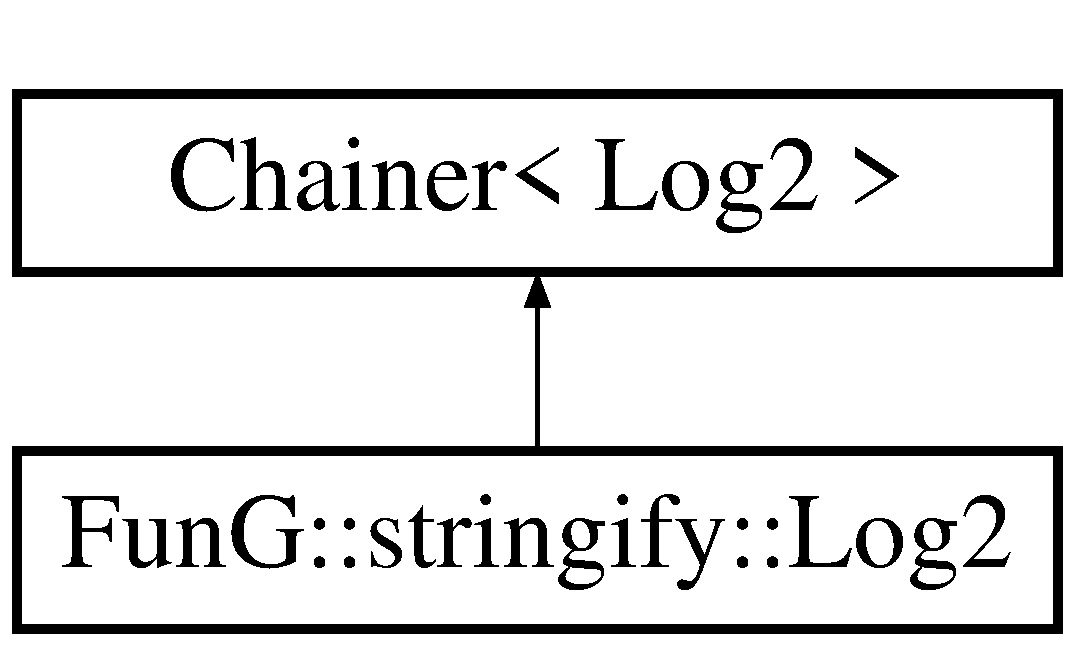
\includegraphics[height=2.000000cm]{structFunG_1_1stringify_1_1Log2}
\end{center}
\end{figure}
\subsection*{Public Member Functions}
\begin{DoxyCompactItemize}
\item 
\hyperlink{structFunG_1_1stringify_1_1Log2_a9ca84817ee0689d515ce529eb596f0ae}{Log2} (const std\-::string \&x=\char`\"{}x\char`\"{})
\begin{DoxyCompactList}\small\item\em Constructor. \end{DoxyCompactList}\item 
void \hyperlink{structFunG_1_1stringify_1_1Log2_a51e1ac2c3bdc5bbcc8684f69c118da4a}{update} (const std\-::string \&x)
\begin{DoxyCompactList}\small\item\em Set point of evaluation. \end{DoxyCompactList}\item 
std\-::string \hyperlink{structFunG_1_1stringify_1_1Log2_ab088996bbeb248688ec005cf608f37bc}{d0} () const noexcept
\begin{DoxyCompactList}\small\item\em Function value. \end{DoxyCompactList}\item 
std\-::string \hyperlink{structFunG_1_1stringify_1_1Log2_a6bdb51218c6412b6c816a9cbb1671383}{d1} (const std\-::string \&dx=\char`\"{}\char`\"{}) const 
\begin{DoxyCompactList}\small\item\em First (directional) derivative. \end{DoxyCompactList}\item 
std\-::string \hyperlink{structFunG_1_1stringify_1_1Log2_a91671f64fa548b8a57ebb2e739655ce2}{d2} (const std\-::string \&dx=\char`\"{}\char`\"{}, const std\-::string \&dy=\char`\"{}\char`\"{}) const 
\begin{DoxyCompactList}\small\item\em Second (directional) derivative. \end{DoxyCompactList}\item 
std\-::string \hyperlink{structFunG_1_1stringify_1_1Log2_a8414dba74d3dd9ae58735bcc6e10123c}{d3} (const std\-::string \&dx=\char`\"{}\char`\"{}, const std\-::string \&dy=\char`\"{}\char`\"{}, const std\-::string \&dz=\char`\"{}\char`\"{}) const 
\begin{DoxyCompactList}\small\item\em Third (directional) derivative. \end{DoxyCompactList}\end{DoxyCompactItemize}


\subsection{Detailed Description}
Base 2 logarithm including first three derivatives. 

For scalar functions directional derivatives are less interesting. Incorporating this function as building block for more complex functions requires directional derivatives. These occur during applications of the chain rule. 

\subsection{Constructor \& Destructor Documentation}
\hypertarget{structFunG_1_1stringify_1_1Log2_a9ca84817ee0689d515ce529eb596f0ae}{\index{Fun\-G\-::stringify\-::\-Log2@{Fun\-G\-::stringify\-::\-Log2}!Log2@{Log2}}
\index{Log2@{Log2}!FunG::stringify::Log2@{Fun\-G\-::stringify\-::\-Log2}}
\subsubsection[{Log2}]{\setlength{\rightskip}{0pt plus 5cm}Fun\-G\-::stringify\-::\-Log2\-::\-Log2 (
\begin{DoxyParamCaption}
\item[{const std\-::string \&}]{x = {\ttfamily \char`\"{}x\char`\"{}}}
\end{DoxyParamCaption}
)\hspace{0.3cm}{\ttfamily [inline]}, {\ttfamily [explicit]}}}\label{structFunG_1_1stringify_1_1Log2_a9ca84817ee0689d515ce529eb596f0ae}


Constructor. 


\begin{DoxyParams}{Parameters}
{\em x} & point of evaluation \\
\hline
\end{DoxyParams}


\subsection{Member Function Documentation}
\hypertarget{structFunG_1_1stringify_1_1Log2_ab088996bbeb248688ec005cf608f37bc}{\index{Fun\-G\-::stringify\-::\-Log2@{Fun\-G\-::stringify\-::\-Log2}!d0@{d0}}
\index{d0@{d0}!FunG::stringify::Log2@{Fun\-G\-::stringify\-::\-Log2}}
\subsubsection[{d0}]{\setlength{\rightskip}{0pt plus 5cm}std\-::string Fun\-G\-::stringify\-::\-Log2\-::d0 (
\begin{DoxyParamCaption}
{}
\end{DoxyParamCaption}
) const\hspace{0.3cm}{\ttfamily [inline]}, {\ttfamily [noexcept]}}}\label{structFunG_1_1stringify_1_1Log2_ab088996bbeb248688ec005cf608f37bc}


Function value. 

\hypertarget{structFunG_1_1stringify_1_1Log2_a6bdb51218c6412b6c816a9cbb1671383}{\index{Fun\-G\-::stringify\-::\-Log2@{Fun\-G\-::stringify\-::\-Log2}!d1@{d1}}
\index{d1@{d1}!FunG::stringify::Log2@{Fun\-G\-::stringify\-::\-Log2}}
\subsubsection[{d1}]{\setlength{\rightskip}{0pt plus 5cm}std\-::string Fun\-G\-::stringify\-::\-Log2\-::d1 (
\begin{DoxyParamCaption}
\item[{const std\-::string \&}]{dx = {\ttfamily \char`\"{}\char`\"{}}}
\end{DoxyParamCaption}
) const\hspace{0.3cm}{\ttfamily [inline]}}}\label{structFunG_1_1stringify_1_1Log2_a6bdb51218c6412b6c816a9cbb1671383}


First (directional) derivative. 

\hypertarget{structFunG_1_1stringify_1_1Log2_a91671f64fa548b8a57ebb2e739655ce2}{\index{Fun\-G\-::stringify\-::\-Log2@{Fun\-G\-::stringify\-::\-Log2}!d2@{d2}}
\index{d2@{d2}!FunG::stringify::Log2@{Fun\-G\-::stringify\-::\-Log2}}
\subsubsection[{d2}]{\setlength{\rightskip}{0pt plus 5cm}std\-::string Fun\-G\-::stringify\-::\-Log2\-::d2 (
\begin{DoxyParamCaption}
\item[{const std\-::string \&}]{dx = {\ttfamily \char`\"{}\char`\"{}}, }
\item[{const std\-::string \&}]{dy = {\ttfamily \char`\"{}\char`\"{}}}
\end{DoxyParamCaption}
) const\hspace{0.3cm}{\ttfamily [inline]}}}\label{structFunG_1_1stringify_1_1Log2_a91671f64fa548b8a57ebb2e739655ce2}


Second (directional) derivative. 

\hypertarget{structFunG_1_1stringify_1_1Log2_a8414dba74d3dd9ae58735bcc6e10123c}{\index{Fun\-G\-::stringify\-::\-Log2@{Fun\-G\-::stringify\-::\-Log2}!d3@{d3}}
\index{d3@{d3}!FunG::stringify::Log2@{Fun\-G\-::stringify\-::\-Log2}}
\subsubsection[{d3}]{\setlength{\rightskip}{0pt plus 5cm}std\-::string Fun\-G\-::stringify\-::\-Log2\-::d3 (
\begin{DoxyParamCaption}
\item[{const std\-::string \&}]{dx = {\ttfamily \char`\"{}\char`\"{}}, }
\item[{const std\-::string \&}]{dy = {\ttfamily \char`\"{}\char`\"{}}, }
\item[{const std\-::string \&}]{dz = {\ttfamily \char`\"{}\char`\"{}}}
\end{DoxyParamCaption}
) const\hspace{0.3cm}{\ttfamily [inline]}}}\label{structFunG_1_1stringify_1_1Log2_a8414dba74d3dd9ae58735bcc6e10123c}


Third (directional) derivative. 

\hypertarget{structFunG_1_1stringify_1_1Log2_a51e1ac2c3bdc5bbcc8684f69c118da4a}{\index{Fun\-G\-::stringify\-::\-Log2@{Fun\-G\-::stringify\-::\-Log2}!update@{update}}
\index{update@{update}!FunG::stringify::Log2@{Fun\-G\-::stringify\-::\-Log2}}
\subsubsection[{update}]{\setlength{\rightskip}{0pt plus 5cm}void Fun\-G\-::stringify\-::\-Log2\-::update (
\begin{DoxyParamCaption}
\item[{const std\-::string \&}]{x}
\end{DoxyParamCaption}
)\hspace{0.3cm}{\ttfamily [inline]}}}\label{structFunG_1_1stringify_1_1Log2_a51e1ac2c3bdc5bbcc8684f69c118da4a}


Set point of evaluation. 



The documentation for this struct was generated from the following file\-:\begin{DoxyCompactItemize}
\item 
include/fung/stringify/cmath/\hyperlink{stringify_2cmath_2log_8hh}{log.\-hh}\end{DoxyCompactItemize}

\hypertarget{structFunG_1_1texify_1_1Log2}{\section{Fun\-G\-:\-:texify\-:\-:Log2 Struct Reference}
\label{structFunG_1_1texify_1_1Log2}\index{Fun\-G\-::texify\-::\-Log2@{Fun\-G\-::texify\-::\-Log2}}
}


Base 2 logarithm including first three derivatives.  




{\ttfamily \#include $<$log.\-hh$>$}

Inheritance diagram for Fun\-G\-:\-:texify\-:\-:Log2\-:\begin{figure}[H]
\begin{center}
\leavevmode
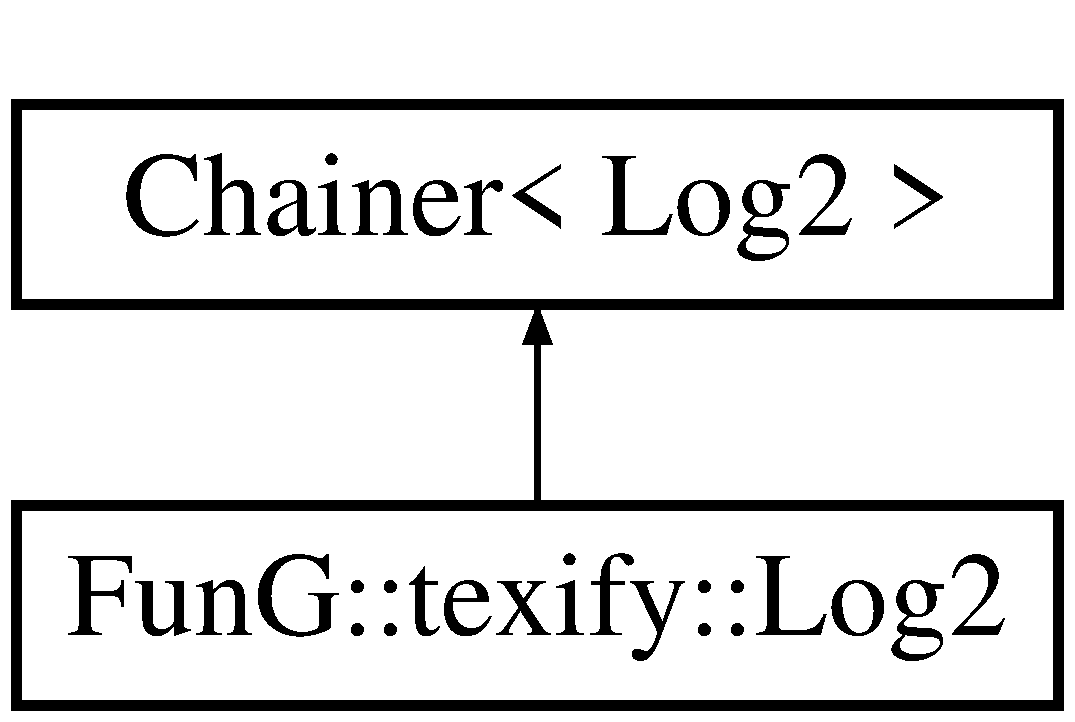
\includegraphics[height=2.000000cm]{structFunG_1_1texify_1_1Log2}
\end{center}
\end{figure}
\subsection*{Public Member Functions}
\begin{DoxyCompactItemize}
\item 
\hyperlink{structFunG_1_1texify_1_1Log2_a5caf39289b9b2df44ab158fe662992b9}{Log2} (const std\-::string \&x=\char`\"{}x\char`\"{})
\begin{DoxyCompactList}\small\item\em Constructor. \end{DoxyCompactList}\item 
void \hyperlink{structFunG_1_1texify_1_1Log2_aa75af872b1a7b0bdaf690297cc2d25de}{update} (const std\-::string \&x)
\begin{DoxyCompactList}\small\item\em Set point of evaluation. \end{DoxyCompactList}\item 
std\-::string \hyperlink{structFunG_1_1texify_1_1Log2_a577fe8797da89bf013cb9a9cb3b9af18}{d0} () const noexcept
\begin{DoxyCompactList}\small\item\em Function value. \end{DoxyCompactList}\item 
std\-::string \hyperlink{structFunG_1_1texify_1_1Log2_a443076997a4d565dbc4ef204131cdf8c}{d1} (const std\-::string \&dx=\char`\"{}\char`\"{}) const 
\begin{DoxyCompactList}\small\item\em First (directional) derivative. \end{DoxyCompactList}\item 
std\-::string \hyperlink{structFunG_1_1texify_1_1Log2_a55e9b2a9b3652896a1767d64304bf427}{d2} (const std\-::string \&dx=\char`\"{}\char`\"{}, const std\-::string \&dy=\char`\"{}\char`\"{}) const 
\begin{DoxyCompactList}\small\item\em Second (directional) derivative. \end{DoxyCompactList}\item 
std\-::string \hyperlink{structFunG_1_1texify_1_1Log2_ab8af458113dd07486e29f7f32287dfa4}{d3} (const std\-::string \&dx=\char`\"{}\char`\"{}, const std\-::string \&dy=\char`\"{}\char`\"{}, const std\-::string \&dz=\char`\"{}\char`\"{}) const 
\begin{DoxyCompactList}\small\item\em Third (directional) derivative. \end{DoxyCompactList}\end{DoxyCompactItemize}


\subsection{Detailed Description}
Base 2 logarithm including first three derivatives. 

For scalar functions directional derivatives are less interesting. Incorporating this function as building block for more complex functions requires directional derivatives. These occur during applications of the chain rule. 

\subsection{Constructor \& Destructor Documentation}
\hypertarget{structFunG_1_1texify_1_1Log2_a5caf39289b9b2df44ab158fe662992b9}{\index{Fun\-G\-::texify\-::\-Log2@{Fun\-G\-::texify\-::\-Log2}!Log2@{Log2}}
\index{Log2@{Log2}!FunG::texify::Log2@{Fun\-G\-::texify\-::\-Log2}}
\subsubsection[{Log2}]{\setlength{\rightskip}{0pt plus 5cm}Fun\-G\-::texify\-::\-Log2\-::\-Log2 (
\begin{DoxyParamCaption}
\item[{const std\-::string \&}]{x = {\ttfamily \char`\"{}x\char`\"{}}}
\end{DoxyParamCaption}
)\hspace{0.3cm}{\ttfamily [inline]}, {\ttfamily [explicit]}}}\label{structFunG_1_1texify_1_1Log2_a5caf39289b9b2df44ab158fe662992b9}


Constructor. 


\begin{DoxyParams}{Parameters}
{\em x} & point of evaluation \\
\hline
\end{DoxyParams}


\subsection{Member Function Documentation}
\hypertarget{structFunG_1_1texify_1_1Log2_a577fe8797da89bf013cb9a9cb3b9af18}{\index{Fun\-G\-::texify\-::\-Log2@{Fun\-G\-::texify\-::\-Log2}!d0@{d0}}
\index{d0@{d0}!FunG::texify::Log2@{Fun\-G\-::texify\-::\-Log2}}
\subsubsection[{d0}]{\setlength{\rightskip}{0pt plus 5cm}std\-::string Fun\-G\-::texify\-::\-Log2\-::d0 (
\begin{DoxyParamCaption}
{}
\end{DoxyParamCaption}
) const\hspace{0.3cm}{\ttfamily [inline]}, {\ttfamily [noexcept]}}}\label{structFunG_1_1texify_1_1Log2_a577fe8797da89bf013cb9a9cb3b9af18}


Function value. 

\hypertarget{structFunG_1_1texify_1_1Log2_a443076997a4d565dbc4ef204131cdf8c}{\index{Fun\-G\-::texify\-::\-Log2@{Fun\-G\-::texify\-::\-Log2}!d1@{d1}}
\index{d1@{d1}!FunG::texify::Log2@{Fun\-G\-::texify\-::\-Log2}}
\subsubsection[{d1}]{\setlength{\rightskip}{0pt plus 5cm}std\-::string Fun\-G\-::texify\-::\-Log2\-::d1 (
\begin{DoxyParamCaption}
\item[{const std\-::string \&}]{dx = {\ttfamily \char`\"{}\char`\"{}}}
\end{DoxyParamCaption}
) const\hspace{0.3cm}{\ttfamily [inline]}}}\label{structFunG_1_1texify_1_1Log2_a443076997a4d565dbc4ef204131cdf8c}


First (directional) derivative. 

\hypertarget{structFunG_1_1texify_1_1Log2_a55e9b2a9b3652896a1767d64304bf427}{\index{Fun\-G\-::texify\-::\-Log2@{Fun\-G\-::texify\-::\-Log2}!d2@{d2}}
\index{d2@{d2}!FunG::texify::Log2@{Fun\-G\-::texify\-::\-Log2}}
\subsubsection[{d2}]{\setlength{\rightskip}{0pt plus 5cm}std\-::string Fun\-G\-::texify\-::\-Log2\-::d2 (
\begin{DoxyParamCaption}
\item[{const std\-::string \&}]{dx = {\ttfamily \char`\"{}\char`\"{}}, }
\item[{const std\-::string \&}]{dy = {\ttfamily \char`\"{}\char`\"{}}}
\end{DoxyParamCaption}
) const\hspace{0.3cm}{\ttfamily [inline]}}}\label{structFunG_1_1texify_1_1Log2_a55e9b2a9b3652896a1767d64304bf427}


Second (directional) derivative. 

\hypertarget{structFunG_1_1texify_1_1Log2_ab8af458113dd07486e29f7f32287dfa4}{\index{Fun\-G\-::texify\-::\-Log2@{Fun\-G\-::texify\-::\-Log2}!d3@{d3}}
\index{d3@{d3}!FunG::texify::Log2@{Fun\-G\-::texify\-::\-Log2}}
\subsubsection[{d3}]{\setlength{\rightskip}{0pt plus 5cm}std\-::string Fun\-G\-::texify\-::\-Log2\-::d3 (
\begin{DoxyParamCaption}
\item[{const std\-::string \&}]{dx = {\ttfamily \char`\"{}\char`\"{}}, }
\item[{const std\-::string \&}]{dy = {\ttfamily \char`\"{}\char`\"{}}, }
\item[{const std\-::string \&}]{dz = {\ttfamily \char`\"{}\char`\"{}}}
\end{DoxyParamCaption}
) const\hspace{0.3cm}{\ttfamily [inline]}}}\label{structFunG_1_1texify_1_1Log2_ab8af458113dd07486e29f7f32287dfa4}


Third (directional) derivative. 

\hypertarget{structFunG_1_1texify_1_1Log2_aa75af872b1a7b0bdaf690297cc2d25de}{\index{Fun\-G\-::texify\-::\-Log2@{Fun\-G\-::texify\-::\-Log2}!update@{update}}
\index{update@{update}!FunG::texify::Log2@{Fun\-G\-::texify\-::\-Log2}}
\subsubsection[{update}]{\setlength{\rightskip}{0pt plus 5cm}void Fun\-G\-::texify\-::\-Log2\-::update (
\begin{DoxyParamCaption}
\item[{const std\-::string \&}]{x}
\end{DoxyParamCaption}
)\hspace{0.3cm}{\ttfamily [inline]}}}\label{structFunG_1_1texify_1_1Log2_aa75af872b1a7b0bdaf690297cc2d25de}


Set point of evaluation. 



The documentation for this struct was generated from the following file\-:\begin{DoxyCompactItemize}
\item 
include/fung/cmath/texify/\hyperlink{texify_2log_8hh}{log.\-hh}\end{DoxyCompactItemize}

\hypertarget{structFunG_1_1MathOpTraits}{\section{Fun\-G\-:\-:Math\-Op\-Traits$<$ T, class $>$ Struct Template Reference}
\label{structFunG_1_1MathOpTraits}\index{Fun\-G\-::\-Math\-Op\-Traits$<$ T, class $>$@{Fun\-G\-::\-Math\-Op\-Traits$<$ T, class $>$}}
}


{\ttfamily \#include $<$mathop\-\_\-traits.\-hh$>$}

\subsection*{Static Public Member Functions}
\begin{DoxyCompactItemize}
\item 
{\footnotesize template$<$class S $>$ }\\static constexpr auto \hyperlink{structFunG_1_1MathOpTraits_aeafa649bb964e8280e50d46bc9de5f48}{multiply} (const T \&lhs, const S \&rhs)
\item 
static constexpr auto \hyperlink{structFunG_1_1MathOpTraits_a41f952d5f51ac17f9ed49218a6894605}{add} (const T \&lhs, const T \&rhs)
\end{DoxyCompactItemize}


\subsection{Member Function Documentation}
\hypertarget{structFunG_1_1MathOpTraits_a41f952d5f51ac17f9ed49218a6894605}{\index{Fun\-G\-::\-Math\-Op\-Traits@{Fun\-G\-::\-Math\-Op\-Traits}!add@{add}}
\index{add@{add}!FunG::MathOpTraits@{Fun\-G\-::\-Math\-Op\-Traits}}
\subsubsection[{add}]{\setlength{\rightskip}{0pt plus 5cm}template$<$class T, class  = void$>$ static constexpr auto {\bf Fun\-G\-::\-Math\-Op\-Traits}$<$ T, class $>$\-::add (
\begin{DoxyParamCaption}
\item[{const T \&}]{lhs, }
\item[{const T \&}]{rhs}
\end{DoxyParamCaption}
)\hspace{0.3cm}{\ttfamily [inline]}, {\ttfamily [static]}}}\label{structFunG_1_1MathOpTraits_a41f952d5f51ac17f9ed49218a6894605}
\hypertarget{structFunG_1_1MathOpTraits_aeafa649bb964e8280e50d46bc9de5f48}{\index{Fun\-G\-::\-Math\-Op\-Traits@{Fun\-G\-::\-Math\-Op\-Traits}!multiply@{multiply}}
\index{multiply@{multiply}!FunG::MathOpTraits@{Fun\-G\-::\-Math\-Op\-Traits}}
\subsubsection[{multiply}]{\setlength{\rightskip}{0pt plus 5cm}template$<$class T, class  = void$>$ template$<$class S $>$ static constexpr auto {\bf Fun\-G\-::\-Math\-Op\-Traits}$<$ T, class $>$\-::multiply (
\begin{DoxyParamCaption}
\item[{const T \&}]{lhs, }
\item[{const S \&}]{rhs}
\end{DoxyParamCaption}
)\hspace{0.3cm}{\ttfamily [inline]}, {\ttfamily [static]}}}\label{structFunG_1_1MathOpTraits_aeafa649bb964e8280e50d46bc9de5f48}


The documentation for this struct was generated from the following file\-:\begin{DoxyCompactItemize}
\item 
include/fung/util/\hyperlink{mathop__traits_8hh}{mathop\-\_\-traits.\-hh}\end{DoxyCompactItemize}

\hypertarget{structFunG_1_1MathOpTraits_3_01std_1_1string_00_01void_01_4}{\section{Fun\-G\-:\-:Math\-Op\-Traits$<$ std\-:\-:string, void $>$ Struct Template Reference}
\label{structFunG_1_1MathOpTraits_3_01std_1_1string_00_01void_01_4}\index{Fun\-G\-::\-Math\-Op\-Traits$<$ std\-::string, void $>$@{Fun\-G\-::\-Math\-Op\-Traits$<$ std\-::string, void $>$}}
}


{\ttfamily \#include $<$string.\-hh$>$}

\subsection*{Static Public Member Functions}
\begin{DoxyCompactItemize}
\item 
static auto \hyperlink{structFunG_1_1MathOpTraits_3_01std_1_1string_00_01void_01_4_aa6807355068e30da33440e446040f5bb}{multiply} (const std\-::string \&lhs, const std\-::string \&rhs)
\item 
{\footnotesize template$<$class S , std\-::enable\-\_\-if\-\_\-t$<$ std\-::is\-\_\-arithmetic$<$ S $>$\-::value $>$ $\ast$  = nullptr$>$ }\\static auto \hyperlink{structFunG_1_1MathOpTraits_3_01std_1_1string_00_01void_01_4_a86b78e911b4a7f31e1e626c75f328460}{multiply} (S lhs, const std\-::string \&rhs)
\item 
{\footnotesize template$<$class S , std\-::enable\-\_\-if\-\_\-t$<$ std\-::is\-\_\-arithmetic$<$ S $>$\-::value $>$ $\ast$  = nullptr$>$ }\\static auto \hyperlink{structFunG_1_1MathOpTraits_3_01std_1_1string_00_01void_01_4_a6481e1b14e056fed96beba96531ac192}{multiply} (const std\-::string \&lhs, S rhs)
\item 
static auto \hyperlink{structFunG_1_1MathOpTraits_3_01std_1_1string_00_01void_01_4_aca8b35c9ba959901550878e22eeeda06}{add} (const std\-::string \&lhs, const std\-::string \&rhs)
\end{DoxyCompactItemize}


\subsection{Member Function Documentation}
\hypertarget{structFunG_1_1MathOpTraits_3_01std_1_1string_00_01void_01_4_aca8b35c9ba959901550878e22eeeda06}{\index{Fun\-G\-::\-Math\-Op\-Traits$<$ std\-::string, void $>$@{Fun\-G\-::\-Math\-Op\-Traits$<$ std\-::string, void $>$}!add@{add}}
\index{add@{add}!FunG::MathOpTraits< std::string, void >@{Fun\-G\-::\-Math\-Op\-Traits$<$ std\-::string, void $>$}}
\subsubsection[{add}]{\setlength{\rightskip}{0pt plus 5cm}static auto {\bf Fun\-G\-::\-Math\-Op\-Traits}$<$ std\-::string, void $>$\-::add (
\begin{DoxyParamCaption}
\item[{const std\-::string \&}]{lhs, }
\item[{const std\-::string \&}]{rhs}
\end{DoxyParamCaption}
)\hspace{0.3cm}{\ttfamily [inline]}, {\ttfamily [static]}}}\label{structFunG_1_1MathOpTraits_3_01std_1_1string_00_01void_01_4_aca8b35c9ba959901550878e22eeeda06}
\hypertarget{structFunG_1_1MathOpTraits_3_01std_1_1string_00_01void_01_4_aa6807355068e30da33440e446040f5bb}{\index{Fun\-G\-::\-Math\-Op\-Traits$<$ std\-::string, void $>$@{Fun\-G\-::\-Math\-Op\-Traits$<$ std\-::string, void $>$}!multiply@{multiply}}
\index{multiply@{multiply}!FunG::MathOpTraits< std::string, void >@{Fun\-G\-::\-Math\-Op\-Traits$<$ std\-::string, void $>$}}
\subsubsection[{multiply}]{\setlength{\rightskip}{0pt plus 5cm}static auto {\bf Fun\-G\-::\-Math\-Op\-Traits}$<$ std\-::string, void $>$\-::multiply (
\begin{DoxyParamCaption}
\item[{const std\-::string \&}]{lhs, }
\item[{const std\-::string \&}]{rhs}
\end{DoxyParamCaption}
)\hspace{0.3cm}{\ttfamily [inline]}, {\ttfamily [static]}}}\label{structFunG_1_1MathOpTraits_3_01std_1_1string_00_01void_01_4_aa6807355068e30da33440e446040f5bb}
\hypertarget{structFunG_1_1MathOpTraits_3_01std_1_1string_00_01void_01_4_a86b78e911b4a7f31e1e626c75f328460}{\index{Fun\-G\-::\-Math\-Op\-Traits$<$ std\-::string, void $>$@{Fun\-G\-::\-Math\-Op\-Traits$<$ std\-::string, void $>$}!multiply@{multiply}}
\index{multiply@{multiply}!FunG::MathOpTraits< std::string, void >@{Fun\-G\-::\-Math\-Op\-Traits$<$ std\-::string, void $>$}}
\subsubsection[{multiply}]{\setlength{\rightskip}{0pt plus 5cm}template$<$class S , std\-::enable\-\_\-if\-\_\-t$<$ std\-::is\-\_\-arithmetic$<$ S $>$\-::value $>$ $\ast$  = nullptr$>$ static auto {\bf Fun\-G\-::\-Math\-Op\-Traits}$<$ std\-::string, void $>$\-::multiply (
\begin{DoxyParamCaption}
\item[{S}]{lhs, }
\item[{const std\-::string \&}]{rhs}
\end{DoxyParamCaption}
)\hspace{0.3cm}{\ttfamily [inline]}, {\ttfamily [static]}}}\label{structFunG_1_1MathOpTraits_3_01std_1_1string_00_01void_01_4_a86b78e911b4a7f31e1e626c75f328460}
\hypertarget{structFunG_1_1MathOpTraits_3_01std_1_1string_00_01void_01_4_a6481e1b14e056fed96beba96531ac192}{\index{Fun\-G\-::\-Math\-Op\-Traits$<$ std\-::string, void $>$@{Fun\-G\-::\-Math\-Op\-Traits$<$ std\-::string, void $>$}!multiply@{multiply}}
\index{multiply@{multiply}!FunG::MathOpTraits< std::string, void >@{Fun\-G\-::\-Math\-Op\-Traits$<$ std\-::string, void $>$}}
\subsubsection[{multiply}]{\setlength{\rightskip}{0pt plus 5cm}template$<$class S , std\-::enable\-\_\-if\-\_\-t$<$ std\-::is\-\_\-arithmetic$<$ S $>$\-::value $>$ $\ast$  = nullptr$>$ static auto {\bf Fun\-G\-::\-Math\-Op\-Traits}$<$ std\-::string, void $>$\-::multiply (
\begin{DoxyParamCaption}
\item[{const std\-::string \&}]{lhs, }
\item[{S}]{rhs}
\end{DoxyParamCaption}
)\hspace{0.3cm}{\ttfamily [inline]}, {\ttfamily [static]}}}\label{structFunG_1_1MathOpTraits_3_01std_1_1string_00_01void_01_4_a6481e1b14e056fed96beba96531ac192}


The documentation for this struct was generated from the following file\-:\begin{DoxyCompactItemize}
\item 
include/fung/util/\hyperlink{string_8hh}{string.\-hh}\end{DoxyCompactItemize}

\hypertarget{structFunG_1_1MathOpTraits_3_01T_00_01std_1_1enable__if__t_3_01std_1_1is__arithmetic_3_01T_01_4_1_1value_01_4_01_4}{}\section{FunG\+:\+:Math\+Op\+Traits$<$ T, std\+:\+:enable\+\_\+if\+\_\+t$<$ std\+:\+:is\+\_\+arithmetic$<$ T $>$\+:\+:value $>$ $>$ Struct Template Reference}
\label{structFunG_1_1MathOpTraits_3_01T_00_01std_1_1enable__if__t_3_01std_1_1is__arithmetic_3_01T_01_4_1_1value_01_4_01_4}\index{Fun\+G\+::\+Math\+Op\+Traits$<$ T, std\+::enable\+\_\+if\+\_\+t$<$ std\+::is\+\_\+arithmetic$<$ T $>$\+::value $>$ $>$@{Fun\+G\+::\+Math\+Op\+Traits$<$ T, std\+::enable\+\_\+if\+\_\+t$<$ std\+::is\+\_\+arithmetic$<$ T $>$\+::value $>$ $>$}}


{\ttfamily \#include $<$mathop\+\_\+traits.\+hh$>$}

\subsection*{Static Public Member Functions}
\begin{DoxyCompactItemize}
\item 
static constexpr auto \hyperlink{structFunG_1_1MathOpTraits_3_01T_00_01std_1_1enable__if__t_3_01std_1_1is__arithmetic_3_01T_01_4_1_1value_01_4_01_4_ac0a15812b088ab59de75d84bd2133489}{multiply} (T lhs, T rhs) noexcept
\item 
static constexpr auto \hyperlink{structFunG_1_1MathOpTraits_3_01T_00_01std_1_1enable__if__t_3_01std_1_1is__arithmetic_3_01T_01_4_1_1value_01_4_01_4_acab509051d7a95f0d58f495641ac9845}{add} (T lhs, T rhs) noexcept
\end{DoxyCompactItemize}


\subsection{Member Function Documentation}
\index{Fun\+G\+::\+Math\+Op\+Traits$<$ T, std\+::enable\+\_\+if\+\_\+t$<$ std\+::is\+\_\+arithmetic$<$ T $>$\+::value $>$ $>$@{Fun\+G\+::\+Math\+Op\+Traits$<$ T, std\+::enable\+\_\+if\+\_\+t$<$ std\+::is\+\_\+arithmetic$<$ T $>$\+::value $>$ $>$}!add@{add}}
\index{add@{add}!Fun\+G\+::\+Math\+Op\+Traits$<$ T, std\+::enable\+\_\+if\+\_\+t$<$ std\+::is\+\_\+arithmetic$<$ T $>$\+::value $>$ $>$@{Fun\+G\+::\+Math\+Op\+Traits$<$ T, std\+::enable\+\_\+if\+\_\+t$<$ std\+::is\+\_\+arithmetic$<$ T $>$\+::value $>$ $>$}}
\subsubsection[{\texorpdfstring{add(\+T lhs, T rhs) noexcept}{add(T lhs, T rhs) noexcept}}]{\setlength{\rightskip}{0pt plus 5cm}template$<$class T $>$ static constexpr auto {\bf Fun\+G\+::\+Math\+Op\+Traits}$<$ T, std\+::enable\+\_\+if\+\_\+t$<$ std\+::is\+\_\+arithmetic$<$ T $>$\+::value $>$ $>$\+::add (
\begin{DoxyParamCaption}
\item[{T}]{lhs, }
\item[{T}]{rhs}
\end{DoxyParamCaption}
)\hspace{0.3cm}{\ttfamily [inline]}, {\ttfamily [static]}, {\ttfamily [noexcept]}}\hypertarget{structFunG_1_1MathOpTraits_3_01T_00_01std_1_1enable__if__t_3_01std_1_1is__arithmetic_3_01T_01_4_1_1value_01_4_01_4_acab509051d7a95f0d58f495641ac9845}{}\label{structFunG_1_1MathOpTraits_3_01T_00_01std_1_1enable__if__t_3_01std_1_1is__arithmetic_3_01T_01_4_1_1value_01_4_01_4_acab509051d7a95f0d58f495641ac9845}
\index{Fun\+G\+::\+Math\+Op\+Traits$<$ T, std\+::enable\+\_\+if\+\_\+t$<$ std\+::is\+\_\+arithmetic$<$ T $>$\+::value $>$ $>$@{Fun\+G\+::\+Math\+Op\+Traits$<$ T, std\+::enable\+\_\+if\+\_\+t$<$ std\+::is\+\_\+arithmetic$<$ T $>$\+::value $>$ $>$}!multiply@{multiply}}
\index{multiply@{multiply}!Fun\+G\+::\+Math\+Op\+Traits$<$ T, std\+::enable\+\_\+if\+\_\+t$<$ std\+::is\+\_\+arithmetic$<$ T $>$\+::value $>$ $>$@{Fun\+G\+::\+Math\+Op\+Traits$<$ T, std\+::enable\+\_\+if\+\_\+t$<$ std\+::is\+\_\+arithmetic$<$ T $>$\+::value $>$ $>$}}
\subsubsection[{\texorpdfstring{multiply(\+T lhs, T rhs) noexcept}{multiply(T lhs, T rhs) noexcept}}]{\setlength{\rightskip}{0pt plus 5cm}template$<$class T $>$ static constexpr auto {\bf Fun\+G\+::\+Math\+Op\+Traits}$<$ T, std\+::enable\+\_\+if\+\_\+t$<$ std\+::is\+\_\+arithmetic$<$ T $>$\+::value $>$ $>$\+::multiply (
\begin{DoxyParamCaption}
\item[{T}]{lhs, }
\item[{T}]{rhs}
\end{DoxyParamCaption}
)\hspace{0.3cm}{\ttfamily [inline]}, {\ttfamily [static]}, {\ttfamily [noexcept]}}\hypertarget{structFunG_1_1MathOpTraits_3_01T_00_01std_1_1enable__if__t_3_01std_1_1is__arithmetic_3_01T_01_4_1_1value_01_4_01_4_ac0a15812b088ab59de75d84bd2133489}{}\label{structFunG_1_1MathOpTraits_3_01T_00_01std_1_1enable__if__t_3_01std_1_1is__arithmetic_3_01T_01_4_1_1value_01_4_01_4_ac0a15812b088ab59de75d84bd2133489}


The documentation for this struct was generated from the following file\+:\begin{DoxyCompactItemize}
\item 
include/fung/util/\hyperlink{mathop__traits_8hh}{mathop\+\_\+traits.\+hh}\end{DoxyCompactItemize}

\hypertarget{structFunG_1_1Concepts_1_1MatrixConcept}{}\section{FunG\+:\+:Concepts\+:\+:Matrix\+Concept Struct Reference}
\label{structFunG_1_1Concepts_1_1MatrixConcept}\index{Fun\+G\+::\+Concepts\+::\+Matrix\+Concept@{Fun\+G\+::\+Concepts\+::\+Matrix\+Concept}}


Requirements for matrices.  




{\ttfamily \#include $<$concepts.\+hh$>$}

Inheritance diagram for FunG\+:\+:Concepts\+:\+:Matrix\+Concept\+:\begin{figure}[H]
\begin{center}
\leavevmode
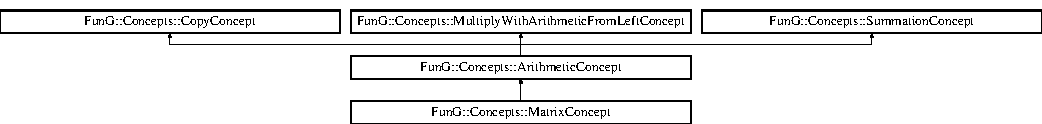
\includegraphics[height=1.661721cm]{structFunG_1_1Concepts_1_1MatrixConcept}
\end{center}
\end{figure}
\subsection*{Public Member Functions}
\begin{DoxyCompactItemize}
\item 
unspecified \hyperlink{structFunG_1_1Concepts_1_1MatrixConcept_ad5d89a552a4dc01fc0d06170cca8f00c}{operator\mbox{[}$\,$\mbox{]}} (int)
\begin{DoxyCompactList}\small\item\em \hyperlink{namespaceFunG_1_1Access}{Access} to row, providing itself the same \hyperlink{structFunG_1_1Concepts_1_1MatrixConcept_ad5d89a552a4dc01fc0d06170cca8f00c}{operator\mbox{[}$\,$\mbox{]}(int)}. \end{DoxyCompactList}\item 
unspecified \hyperlink{structFunG_1_1Concepts_1_1MatrixConcept_a9a7fc91f16e1ddc5801c37f2bfd1bf47}{operator()} (int, int)
\begin{DoxyCompactList}\small\item\em \hyperlink{namespaceFunG_1_1Access}{Access} to entry. \end{DoxyCompactList}\end{DoxyCompactItemize}


\subsection{Detailed Description}
Requirements for matrices. 

\hyperlink{namespaceFunG_1_1Access}{Access} to matrix elements must be possible either via A\mbox{[}i\mbox{]}\mbox{[}j\mbox{]} or A(i,j). Moreover the requirements of \hyperlink{structFunG_1_1Concepts_1_1ArithmeticConcept}{Arithmetic\+Concept} must be satisfied. 

\subsection{Member Function Documentation}
\index{Fun\+G\+::\+Concepts\+::\+Matrix\+Concept@{Fun\+G\+::\+Concepts\+::\+Matrix\+Concept}!operator()@{operator()}}
\index{operator()@{operator()}!Fun\+G\+::\+Concepts\+::\+Matrix\+Concept@{Fun\+G\+::\+Concepts\+::\+Matrix\+Concept}}
\subsubsection[{\texorpdfstring{operator()(int, int)}{operator()(int, int)}}]{\setlength{\rightskip}{0pt plus 5cm}unspecified Fun\+G\+::\+Concepts\+::\+Matrix\+Concept\+::operator() (
\begin{DoxyParamCaption}
\item[{int}]{, }
\item[{int}]{}
\end{DoxyParamCaption}
)}\hypertarget{structFunG_1_1Concepts_1_1MatrixConcept_a9a7fc91f16e1ddc5801c37f2bfd1bf47}{}\label{structFunG_1_1Concepts_1_1MatrixConcept_a9a7fc91f16e1ddc5801c37f2bfd1bf47}


\hyperlink{namespaceFunG_1_1Access}{Access} to entry. 

\index{Fun\+G\+::\+Concepts\+::\+Matrix\+Concept@{Fun\+G\+::\+Concepts\+::\+Matrix\+Concept}!operator\mbox{[}$\,$\mbox{]}@{operator[]}}
\index{operator\mbox{[}$\,$\mbox{]}@{operator[]}!Fun\+G\+::\+Concepts\+::\+Matrix\+Concept@{Fun\+G\+::\+Concepts\+::\+Matrix\+Concept}}
\subsubsection[{\texorpdfstring{operator[](int)}{operator[](int)}}]{\setlength{\rightskip}{0pt plus 5cm}unspecified Fun\+G\+::\+Concepts\+::\+Matrix\+Concept\+::operator\mbox{[}$\,$\mbox{]} (
\begin{DoxyParamCaption}
\item[{int}]{}
\end{DoxyParamCaption}
)}\hypertarget{structFunG_1_1Concepts_1_1MatrixConcept_ad5d89a552a4dc01fc0d06170cca8f00c}{}\label{structFunG_1_1Concepts_1_1MatrixConcept_ad5d89a552a4dc01fc0d06170cca8f00c}


\hyperlink{namespaceFunG_1_1Access}{Access} to row, providing itself the same \hyperlink{structFunG_1_1Concepts_1_1MatrixConcept_ad5d89a552a4dc01fc0d06170cca8f00c}{operator\mbox{[}$\,$\mbox{]}(int)}. 



The documentation for this struct was generated from the following file\+:\begin{DoxyCompactItemize}
\item 
fung/\hyperlink{concepts_8hh}{concepts.\+hh}\end{DoxyCompactItemize}

\hypertarget{structFunG_1_1Concepts_1_1MatrixConceptCheck}{\section{Fun\-G\-:\-:Concepts\-:\-:Matrix\-Concept\-Check$<$ Matrix $>$ Struct Template Reference}
\label{structFunG_1_1Concepts_1_1MatrixConceptCheck}\index{Fun\-G\-::\-Concepts\-::\-Matrix\-Concept\-Check$<$ Matrix $>$@{Fun\-G\-::\-Concepts\-::\-Matrix\-Concept\-Check$<$ Matrix $>$}}
}


Static check if the requirements of \hyperlink{structFunG_1_1Concepts_1_1MatrixConcept}{Matrix\-Concept} are satisfied.  




{\ttfamily \#include $<$concept\-\_\-check.\-hh$>$}

Inheritance diagram for Fun\-G\-:\-:Concepts\-:\-:Matrix\-Concept\-Check$<$ Matrix $>$\-:\begin{figure}[H]
\begin{center}
\leavevmode
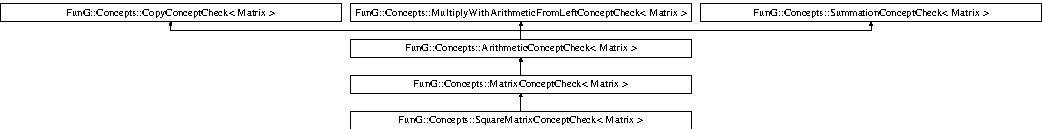
\includegraphics[height=1.728395cm]{structFunG_1_1Concepts_1_1MatrixConceptCheck}
\end{center}
\end{figure}


\subsection{Detailed Description}
\subsubsection*{template$<$class Matrix$>$struct Fun\-G\-::\-Concepts\-::\-Matrix\-Concept\-Check$<$ Matrix $>$}

Static check if the requirements of \hyperlink{structFunG_1_1Concepts_1_1MatrixConcept}{Matrix\-Concept} are satisfied. 

The documentation for this struct was generated from the following file\-:\begin{DoxyCompactItemize}
\item 
fung/concept\-\_\-check.\-hh\end{DoxyCompactItemize}

\hypertarget{structFunG_1_1Concepts_1_1MultiplicationConcept}{\section{\-Fun\-G\-:\-:\-Concepts\-:\-:\-Multiplication\-Concept \-Struct \-Reference}
\label{structFunG_1_1Concepts_1_1MultiplicationConcept}\index{\-Fun\-G\-::\-Concepts\-::\-Multiplication\-Concept@{\-Fun\-G\-::\-Concepts\-::\-Multiplication\-Concept}}
}


\-Requires that multiplication can be performed.  




{\ttfamily \#include $<$concepts.\-hh$>$}

\subsection*{\-Public \-Member \-Functions}
\begin{DoxyCompactItemize}
\item 
unspecified \hyperlink{structFunG_1_1Concepts_1_1MultiplicationConcept_ac91bb184ac3641bb86e8cc03497988f4}{operator$\ast$=} (\-Arg2)
\begin{DoxyCompactList}\small\item\em \-In-\/place multiplication. \-Return type is not checked to support lazy evaluation. \end{DoxyCompactList}\item 
unspecified \hyperlink{structFunG_1_1Concepts_1_1MultiplicationConcept_aaf1220bf588863cbfe3166f216b8422c}{rightmultiplyany} (\-Arg2)
\begin{DoxyCompactList}\small\item\em \-Multiplication via \hyperlink{structFunG_1_1Concepts_1_1MultiplicationConcept_aaf1220bf588863cbfe3166f216b8422c}{rightmultiplyany(\-Arg2)}. \-Return type is not checked to support lazy evaluation. \end{DoxyCompactList}\end{DoxyCompactItemize}


\subsection{\-Detailed \-Description}
\-Requires that multiplication can be performed. 

\-Requires that either a free operator$\ast$(\-Arg1,\-Arg2) exists for multiplication or \-Arg1 provides either the in-\/place multiplication \hyperlink{structFunG_1_1Concepts_1_1MultiplicationConcept_ac91bb184ac3641bb86e8cc03497988f4}{operator$\ast$=(\-Arg2)} or the member function \hyperlink{structFunG_1_1Concepts_1_1MultiplicationConcept_aaf1220bf588863cbfe3166f216b8422c}{rightmultiplyany(\-Arg2)}. 

\subsection{\-Member \-Function \-Documentation}
\hypertarget{structFunG_1_1Concepts_1_1MultiplicationConcept_ac91bb184ac3641bb86e8cc03497988f4}{\index{\-Fun\-G\-::\-Concepts\-::\-Multiplication\-Concept@{\-Fun\-G\-::\-Concepts\-::\-Multiplication\-Concept}!operator$\ast$=@{operator$\ast$=}}
\index{operator$\ast$=@{operator$\ast$=}!FunG::Concepts::MultiplicationConcept@{\-Fun\-G\-::\-Concepts\-::\-Multiplication\-Concept}}
\subsubsection[{operator$\ast$=}]{\setlength{\rightskip}{0pt plus 5cm}unspecified \-Fun\-G\-::\-Concepts\-::\-Multiplication\-Concept\-::operator$\ast$= (
\begin{DoxyParamCaption}
\item[{\-Arg2}]{}
\end{DoxyParamCaption}
)}}\label{structFunG_1_1Concepts_1_1MultiplicationConcept_ac91bb184ac3641bb86e8cc03497988f4}


\-In-\/place multiplication. \-Return type is not checked to support lazy evaluation. 

\hypertarget{structFunG_1_1Concepts_1_1MultiplicationConcept_aaf1220bf588863cbfe3166f216b8422c}{\index{\-Fun\-G\-::\-Concepts\-::\-Multiplication\-Concept@{\-Fun\-G\-::\-Concepts\-::\-Multiplication\-Concept}!rightmultiplyany@{rightmultiplyany}}
\index{rightmultiplyany@{rightmultiplyany}!FunG::Concepts::MultiplicationConcept@{\-Fun\-G\-::\-Concepts\-::\-Multiplication\-Concept}}
\subsubsection[{rightmultiplyany}]{\setlength{\rightskip}{0pt plus 5cm}unspecified {\bf \-Fun\-G\-::\-Concepts\-::\-Multiplication\-Concept\-::rightmultiplyany} (
\begin{DoxyParamCaption}
\item[{\-Arg2}]{}
\end{DoxyParamCaption}
)}}\label{structFunG_1_1Concepts_1_1MultiplicationConcept_aaf1220bf588863cbfe3166f216b8422c}


\-Multiplication via \hyperlink{structFunG_1_1Concepts_1_1MultiplicationConcept_aaf1220bf588863cbfe3166f216b8422c}{rightmultiplyany(\-Arg2)}. \-Return type is not checked to support lazy evaluation. 



\-The documentation for this struct was generated from the following file\-:\begin{DoxyCompactItemize}
\item 
fung/\hyperlink{concepts_8hh}{concepts.\-hh}\end{DoxyCompactItemize}

\hypertarget{structFunG_1_1Concepts_1_1MultiplicationConceptCheck}{}\section{FunG\+:\+:Concepts\+:\+:Multiplication\+Concept\+Check$<$ Arg1, Arg2 $>$ Struct Template Reference}
\label{structFunG_1_1Concepts_1_1MultiplicationConceptCheck}\index{Fun\+G\+::\+Concepts\+::\+Multiplication\+Concept\+Check$<$ Arg1, Arg2 $>$@{Fun\+G\+::\+Concepts\+::\+Multiplication\+Concept\+Check$<$ Arg1, Arg2 $>$}}


Static check if the requirements of \hyperlink{structFunG_1_1Concepts_1_1MultiplicationConcept}{Multiplication\+Concept} are satisfied.  




{\ttfamily \#include $<$concept\+\_\+check.\+hh$>$}



\subsection{Detailed Description}
\subsubsection*{template$<$class Arg1, class Arg2$>$\\*
struct Fun\+G\+::\+Concepts\+::\+Multiplication\+Concept\+Check$<$ Arg1, Arg2 $>$}

Static check if the requirements of \hyperlink{structFunG_1_1Concepts_1_1MultiplicationConcept}{Multiplication\+Concept} are satisfied. 

The documentation for this struct was generated from the following file\+:\begin{DoxyCompactItemize}
\item 
fung/\hyperlink{concept__check_8hh}{concept\+\_\+check.\+hh}\end{DoxyCompactItemize}

\hypertarget{structFunG_1_1Concepts_1_1MultiplyWithArithmeticFromLeftConcept}{\section{Fun\-G\-:\-:Concepts\-:\-:Multiply\-With\-Arithmetic\-From\-Left\-Concept Struct Reference}
\label{structFunG_1_1Concepts_1_1MultiplyWithArithmeticFromLeftConcept}\index{Fun\-G\-::\-Concepts\-::\-Multiply\-With\-Arithmetic\-From\-Left\-Concept@{Fun\-G\-::\-Concepts\-::\-Multiply\-With\-Arithmetic\-From\-Left\-Concept}}
}


Requires that multiplication with double and int can be performed either by in-\/place multiplication or by multiplication from the left.  




{\ttfamily \#include $<$concepts.\-hh$>$}

Inheritance diagram for Fun\-G\-:\-:Concepts\-:\-:Multiply\-With\-Arithmetic\-From\-Left\-Concept\-:\begin{figure}[H]
\begin{center}
\leavevmode
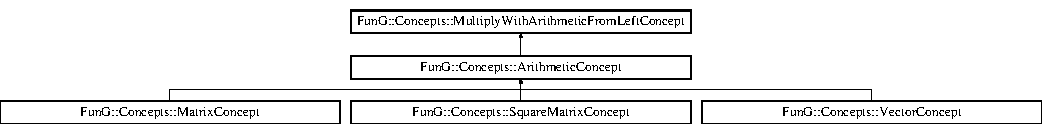
\includegraphics[height=1.661721cm]{structFunG_1_1Concepts_1_1MultiplyWithArithmeticFromLeftConcept}
\end{center}
\end{figure}
\subsection*{Public Member Functions}
\begin{DoxyCompactItemize}
\item 
\hypertarget{structFunG_1_1Concepts_1_1MultiplyWithArithmeticFromLeftConcept_aed5d281f1a44a60696bc512766a42b56}{unspecified \hyperlink{structFunG_1_1Concepts_1_1MultiplyWithArithmeticFromLeftConcept_aed5d281f1a44a60696bc512766a42b56}{operator$\ast$=} (double)}\label{structFunG_1_1Concepts_1_1MultiplyWithArithmeticFromLeftConcept_aed5d281f1a44a60696bc512766a42b56}

\begin{DoxyCompactList}\small\item\em In-\/place multiplication. Return type is not checked to support lazy evaluation. \end{DoxyCompactList}\item 
\hypertarget{structFunG_1_1Concepts_1_1MultiplyWithArithmeticFromLeftConcept_a3a7792406c3e6eb824b8f170b825a1d8}{unspecified \hyperlink{structFunG_1_1Concepts_1_1MultiplyWithArithmeticFromLeftConcept_a3a7792406c3e6eb824b8f170b825a1d8}{operator$\ast$=} (int)}\label{structFunG_1_1Concepts_1_1MultiplyWithArithmeticFromLeftConcept_a3a7792406c3e6eb824b8f170b825a1d8}

\begin{DoxyCompactList}\small\item\em In-\/place multiplication. Return type is not checked to support lazy evaluation. \end{DoxyCompactList}\end{DoxyCompactItemize}


\subsection{Detailed Description}
Requires that multiplication with double and int can be performed either by in-\/place multiplication or by multiplication from the left. 


\begin{DoxyTemplParams}{Template Parameters}
{\em Arg} & type to check \\
\hline
\end{DoxyTemplParams}


The documentation for this struct was generated from the following file\-:\begin{DoxyCompactItemize}
\item 
Fun\-G/\hyperlink{concepts_8hh}{concepts.\-hh}\end{DoxyCompactItemize}

\hypertarget{structFunG_1_1Concepts_1_1MultiplyWithArithmeticFromLeftConceptCheck}{\section{Fun\-G\-:\-:Concepts\-:\-:Multiply\-With\-Arithmetic\-From\-Left\-Concept\-Check$<$ Arg $>$ Struct Template Reference}
\label{structFunG_1_1Concepts_1_1MultiplyWithArithmeticFromLeftConceptCheck}\index{Fun\-G\-::\-Concepts\-::\-Multiply\-With\-Arithmetic\-From\-Left\-Concept\-Check$<$ Arg $>$@{Fun\-G\-::\-Concepts\-::\-Multiply\-With\-Arithmetic\-From\-Left\-Concept\-Check$<$ Arg $>$}}
}


Static check if the requirements of \hyperlink{structFunG_1_1Concepts_1_1MultiplyWithArithmeticFromLeftConcept}{Multiply\-With\-Arithmetic\-From\-Left\-Concept} are satisfied.  




{\ttfamily \#include $<$concept\-\_\-check.\-hh$>$}

Inheritance diagram for Fun\-G\-:\-:Concepts\-:\-:Multiply\-With\-Arithmetic\-From\-Left\-Concept\-Check$<$ Arg $>$\-:\begin{figure}[H]
\begin{center}
\leavevmode
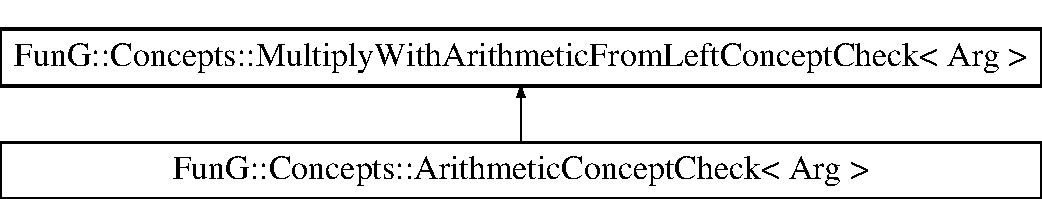
\includegraphics[height=2.000000cm]{structFunG_1_1Concepts_1_1MultiplyWithArithmeticFromLeftConceptCheck}
\end{center}
\end{figure}


\subsection{Detailed Description}
\subsubsection*{template$<$class Arg$>$struct Fun\-G\-::\-Concepts\-::\-Multiply\-With\-Arithmetic\-From\-Left\-Concept\-Check$<$ Arg $>$}

Static check if the requirements of \hyperlink{structFunG_1_1Concepts_1_1MultiplyWithArithmeticFromLeftConcept}{Multiply\-With\-Arithmetic\-From\-Left\-Concept} are satisfied. 

The documentation for this struct was generated from the following file\-:\begin{DoxyCompactItemize}
\item 
fung/\hyperlink{concept__check_8hh}{concept\-\_\-check.\-hh}\end{DoxyCompactItemize}

\hypertarget{classFunG_1_1NonSymmetricMatrixException}{}\section{Fun\+G\+:\+:Non\+Symmetric\+Matrix\+Exception Class Reference}
\label{classFunG_1_1NonSymmetricMatrixException}\index{Fun\+G\+::\+Non\+Symmetric\+Matrix\+Exception@{Fun\+G\+::\+Non\+Symmetric\+Matrix\+Exception}}


Exception for non-\/symmetric matrices if symmetric matrices are required.  




{\ttfamily \#include $<$exceptions.\+hh$>$}

Inheritance diagram for Fun\+G\+:\+:Non\+Symmetric\+Matrix\+Exception\+:\begin{figure}[H]
\begin{center}
\leavevmode
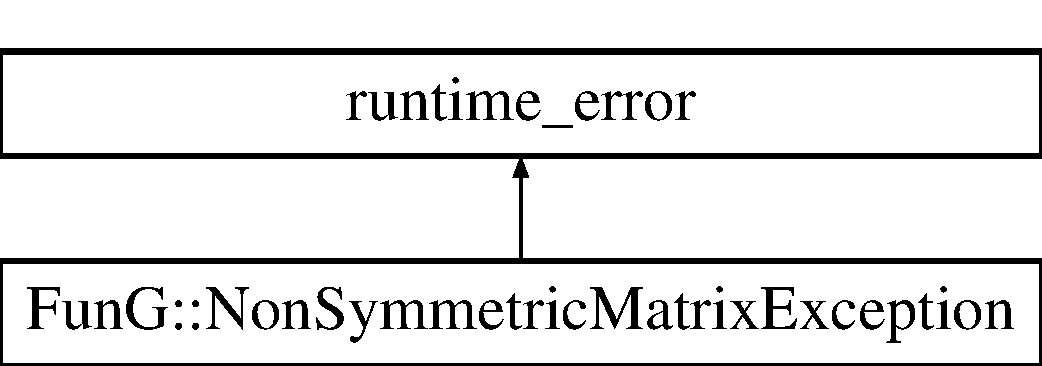
\includegraphics[height=2.000000cm]{classFunG_1_1NonSymmetricMatrixException}
\end{center}
\end{figure}
\subsection*{Public Member Functions}
\begin{DoxyCompactItemize}
\item 
{\footnotesize template$<$class Value , class  = std\+::enable\+\_\+if\+\_\+t$<$std\+::is\+\_\+arithmetic$<$\+Value$>$\+::value$>$$>$ }\\\hyperlink{classFunG_1_1NonSymmetricMatrixException_a1c11fd643c37e5fa2145aba2cc7ab09d}{Non\+Symmetric\+Matrix\+Exception} (const std\+::string \&function, const Value \&rows, const Value \&cols, const std\+::string \&file, const int line)
\begin{DoxyCompactList}\small\item\em Constructor. \end{DoxyCompactList}\end{DoxyCompactItemize}


\subsection{Detailed Description}
Exception for non-\/symmetric matrices if symmetric matrices are required. 

\subsection{Constructor \& Destructor Documentation}
\hypertarget{classFunG_1_1NonSymmetricMatrixException_a1c11fd643c37e5fa2145aba2cc7ab09d}{}\index{Fun\+G\+::\+Non\+Symmetric\+Matrix\+Exception@{Fun\+G\+::\+Non\+Symmetric\+Matrix\+Exception}!Non\+Symmetric\+Matrix\+Exception@{Non\+Symmetric\+Matrix\+Exception}}
\index{Non\+Symmetric\+Matrix\+Exception@{Non\+Symmetric\+Matrix\+Exception}!Fun\+G\+::\+Non\+Symmetric\+Matrix\+Exception@{Fun\+G\+::\+Non\+Symmetric\+Matrix\+Exception}}
\subsubsection[{Non\+Symmetric\+Matrix\+Exception}]{\setlength{\rightskip}{0pt plus 5cm}template$<$class Value , class  = std\+::enable\+\_\+if\+\_\+t$<$std\+::is\+\_\+arithmetic$<$\+Value$>$\+::value$>$$>$ Fun\+G\+::\+Non\+Symmetric\+Matrix\+Exception\+::\+Non\+Symmetric\+Matrix\+Exception (
\begin{DoxyParamCaption}
\item[{const std\+::string \&}]{function, }
\item[{const Value \&}]{rows, }
\item[{const Value \&}]{cols, }
\item[{const std\+::string \&}]{file, }
\item[{const int}]{line}
\end{DoxyParamCaption}
)\hspace{0.3cm}{\ttfamily [inline]}}\label{classFunG_1_1NonSymmetricMatrixException_a1c11fd643c37e5fa2145aba2cc7ab09d}


Constructor. 


\begin{DoxyParams}{Parameters}
{\em function} & name of the function throwing this exception \\
\hline
{\em rows} & number of rows of matrix \\
\hline
{\em cols} & number of columns of matrix \\
\hline
{\em file} & file containing the throwing code \\
\hline
{\em line} & line containing the throwing code \\
\hline
\end{DoxyParams}


The documentation for this class was generated from the following file\+:\begin{DoxyCompactItemize}
\item 
fung/util/\hyperlink{exceptions_8hh}{exceptions.\+hh}\end{DoxyCompactItemize}

\hypertarget{structFunG_1_1LinearAlgebra_1_1NumberOfColumns}{\section{Fun\-G\-:\-:Linear\-Algebra\-:\-:Number\-Of\-Columns$<$ Matrix, class $>$ Struct Template Reference}
\label{structFunG_1_1LinearAlgebra_1_1NumberOfColumns}\index{Fun\-G\-::\-Linear\-Algebra\-::\-Number\-Of\-Columns$<$ Matrix, class $>$@{Fun\-G\-::\-Linear\-Algebra\-::\-Number\-Of\-Columns$<$ Matrix, class $>$}}
}


Specialize this for your matrix class. Number of columns must be provided by a static member variable called value.  




{\ttfamily \#include $<$extract\-\_\-rows\-\_\-and\-\_\-cols.\-hh$>$}

Inheritance diagram for Fun\-G\-:\-:Linear\-Algebra\-:\-:Number\-Of\-Columns$<$ Matrix, class $>$\-:\begin{figure}[H]
\begin{center}
\leavevmode
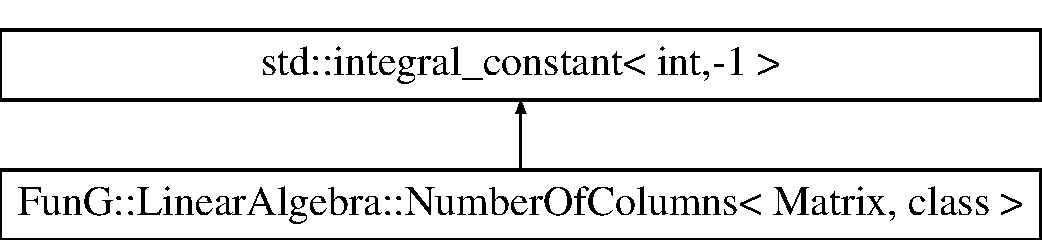
\includegraphics[height=2.000000cm]{structFunG_1_1LinearAlgebra_1_1NumberOfColumns}
\end{center}
\end{figure}


\subsection{Detailed Description}
\subsubsection*{template$<$class Matrix, class = Concepts\-::\-Matrix\-Concept\-Check$<$\-Matrix$>$$>$struct Fun\-G\-::\-Linear\-Algebra\-::\-Number\-Of\-Columns$<$ Matrix, class $>$}

Specialize this for your matrix class. Number of columns must be provided by a static member variable called value. 

The documentation for this struct was generated from the following file\-:\begin{DoxyCompactItemize}
\item 
include/fung/util/\hyperlink{extract__rows__and__cols_8hh}{extract\-\_\-rows\-\_\-and\-\_\-cols.\-hh}\end{DoxyCompactItemize}

\hypertarget{structFunG_1_1LinearAlgebra_1_1NumberOfRows}{}\section{Fun\+G\+:\+:Linear\+Algebra\+:\+:Number\+Of\+Rows$<$ Matrix, class $>$ Struct Template Reference}
\label{structFunG_1_1LinearAlgebra_1_1NumberOfRows}\index{Fun\+G\+::\+Linear\+Algebra\+::\+Number\+Of\+Rows$<$ Matrix, class $>$@{Fun\+G\+::\+Linear\+Algebra\+::\+Number\+Of\+Rows$<$ Matrix, class $>$}}


Specialize this for your matrix class. Number of rows must be provided by a static member variable called value.  




{\ttfamily \#include $<$extract\+\_\+rows\+\_\+and\+\_\+cols.\+hh$>$}

Inheritance diagram for Fun\+G\+:\+:Linear\+Algebra\+:\+:Number\+Of\+Rows$<$ Matrix, class $>$\+:\begin{figure}[H]
\begin{center}
\leavevmode
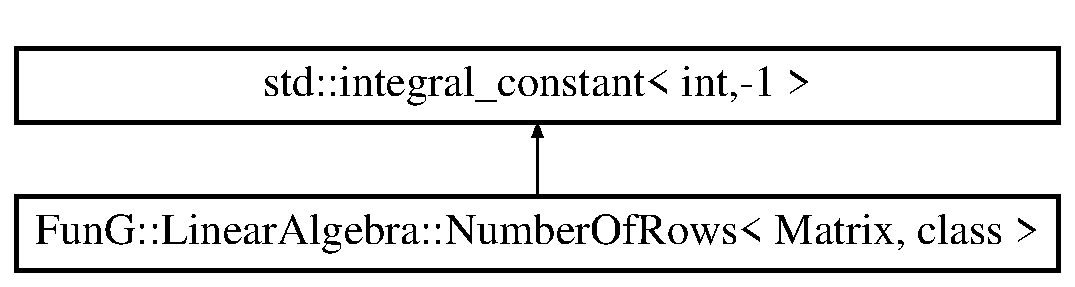
\includegraphics[height=2.000000cm]{structFunG_1_1LinearAlgebra_1_1NumberOfRows}
\end{center}
\end{figure}


\subsection{Detailed Description}
\subsubsection*{template$<$class Matrix, class = Concepts\+::\+Matrix\+Concept\+Check$<$\+Matrix$>$$>$struct Fun\+G\+::\+Linear\+Algebra\+::\+Number\+Of\+Rows$<$ Matrix, class $>$}

Specialize this for your matrix class. Number of rows must be provided by a static member variable called value. 

The documentation for this struct was generated from the following file\+:\begin{DoxyCompactItemize}
\item 
fung/util/\hyperlink{extract__rows__and__cols_8hh}{extract\+\_\+rows\+\_\+and\+\_\+cols.\+hh}\end{DoxyCompactItemize}

\hypertarget{classFunG_1_1OutOfDomainException}{}\section{FunG\+:\+:Out\+Of\+Domain\+Exception Class Reference}
\label{classFunG_1_1OutOfDomainException}\index{Fun\+G\+::\+Out\+Of\+Domain\+Exception@{Fun\+G\+::\+Out\+Of\+Domain\+Exception}}


Exception for scalar function arguments that are outside the domain of the function.  




{\ttfamily \#include $<$exceptions.\+hh$>$}

Inheritance diagram for FunG\+:\+:Out\+Of\+Domain\+Exception\+:\begin{figure}[H]
\begin{center}
\leavevmode
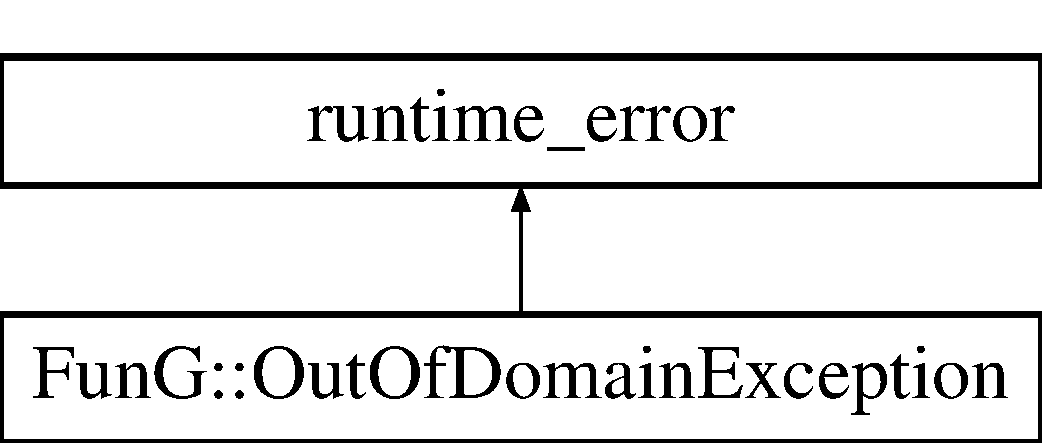
\includegraphics[height=2.000000cm]{classFunG_1_1OutOfDomainException}
\end{center}
\end{figure}
\subsection*{Public Member Functions}
\begin{DoxyCompactItemize}
\item 
{\footnotesize template$<$class Value , class  = std\+::enable\+\_\+if\+\_\+t$<$std\+::is\+\_\+arithmetic$<$\+Value$>$\+::value$>$$>$ }\\\hyperlink{classFunG_1_1OutOfDomainException_ab5dcdcbbe00be01b008e1945a1504d1b}{Out\+Of\+Domain\+Exception} (const std\+::string \&function, const std\+::string \&range, const Value \&value, const std\+::string \&file, const int line)
\begin{DoxyCompactList}\small\item\em Constructor. \end{DoxyCompactList}\end{DoxyCompactItemize}


\subsection{Detailed Description}
Exception for scalar function arguments that are outside the domain of the function. 

Example\+: 
\begin{DoxyCode}
\textcolor{keywordflow}{if}( x < 0 )
  \textcolor{keywordflow}{throw} \hyperlink{classFunG_1_1OutOfDomainException_ab5dcdcbbe00be01b008e1945a1504d1b}{OutOfDomainException}(\textcolor{stringliteral}{"[0,inf["},\textcolor{stringliteral}{"Sqrt"} x,\_\_FILE\_\_,\_\_LINE\_\_);
\end{DoxyCode}
 

\subsection{Constructor \& Destructor Documentation}
\index{Fun\+G\+::\+Out\+Of\+Domain\+Exception@{Fun\+G\+::\+Out\+Of\+Domain\+Exception}!Out\+Of\+Domain\+Exception@{Out\+Of\+Domain\+Exception}}
\index{Out\+Of\+Domain\+Exception@{Out\+Of\+Domain\+Exception}!Fun\+G\+::\+Out\+Of\+Domain\+Exception@{Fun\+G\+::\+Out\+Of\+Domain\+Exception}}
\subsubsection[{\texorpdfstring{Out\+Of\+Domain\+Exception(const std\+::string \&function, const std\+::string \&range, const Value \&value, const std\+::string \&file, const int line)}{OutOfDomainException(const std::string &function, const std::string &range, const Value &value, const std::string &file, const int line)}}]{\setlength{\rightskip}{0pt plus 5cm}template$<$class Value , class  = std\+::enable\+\_\+if\+\_\+t$<$std\+::is\+\_\+arithmetic$<$\+Value$>$\+::value$>$$>$ Fun\+G\+::\+Out\+Of\+Domain\+Exception\+::\+Out\+Of\+Domain\+Exception (
\begin{DoxyParamCaption}
\item[{const std\+::string \&}]{function, }
\item[{const std\+::string \&}]{range, }
\item[{const Value \&}]{value, }
\item[{const std\+::string \&}]{file, }
\item[{const int}]{line}
\end{DoxyParamCaption}
)\hspace{0.3cm}{\ttfamily [inline]}}\hypertarget{classFunG_1_1OutOfDomainException_ab5dcdcbbe00be01b008e1945a1504d1b}{}\label{classFunG_1_1OutOfDomainException_ab5dcdcbbe00be01b008e1945a1504d1b}


Constructor. 


\begin{DoxyParams}{Parameters}
{\em range} & std\+::string that contains the mathematical expression for the valid range \\
\hline
{\em function} & name of the function throwing this exception \\
\hline
{\em value} & value outside range \\
\hline
{\em file} & file containing the throwing code \\
\hline
{\em line} & line containing the throwing code \\
\hline
\end{DoxyParams}


The documentation for this class was generated from the following file\+:\begin{DoxyCompactItemize}
\item 
fung/util/\hyperlink{exceptions_8hh}{exceptions.\+hh}\end{DoxyCompactItemize}

\hypertarget{structFunG_1_1Pow}{\section{Fun\-G\-:\-:Pow$<$ dividend, divisor $>$ Struct Template Reference}
\label{structFunG_1_1Pow}\index{Fun\-G\-::\-Pow$<$ dividend, divisor $>$@{Fun\-G\-::\-Pow$<$ dividend, divisor $>$}}
}


Power function with rational exponent $ k = \frac{dividend}{divisor} $ including first three derivatives.  




{\ttfamily \#include $<$pow.\-hh$>$}

Inheritance diagram for Fun\-G\-:\-:Pow$<$ dividend, divisor $>$\-:\begin{figure}[H]
\begin{center}
\leavevmode
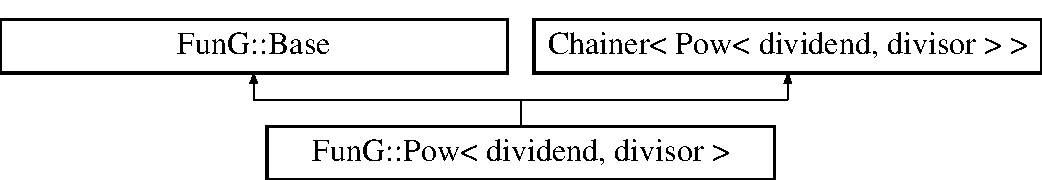
\includegraphics[height=2.000000cm]{structFunG_1_1Pow}
\end{center}
\end{figure}
\subsection*{Public Member Functions}
\begin{DoxyCompactItemize}
\item 
\hyperlink{structFunG_1_1Pow_a80be1d3a5c208e7ac74efa7ff3a7a18f}{Pow} (double x=1)
\begin{DoxyCompactList}\small\item\em Constructor. \end{DoxyCompactList}\item 
void \hyperlink{structFunG_1_1Pow_a2cb004b3cb89c4887b67eb8e666f4852}{update} (double x)
\begin{DoxyCompactList}\small\item\em Set point of evaluation. \end{DoxyCompactList}\item 
double \hyperlink{structFunG_1_1Pow_a840ccc0dbcfabc71863d2932074b955a}{d0} () const noexcept
\begin{DoxyCompactList}\small\item\em Function value. \end{DoxyCompactList}\item 
double \hyperlink{structFunG_1_1Pow_a9e1301ef812a58af196556bc2b33b7c0}{d1} (double dx=1.) const 
\begin{DoxyCompactList}\small\item\em First (directional) derivative. \end{DoxyCompactList}\item 
double \hyperlink{structFunG_1_1Pow_ac3b7b762a8609b5c2ea57831acd04870}{d2} (double dx=1., double dy=1.) const 
\begin{DoxyCompactList}\small\item\em Second (directional) derivative. \end{DoxyCompactList}\item 
double \hyperlink{structFunG_1_1Pow_a5ad0887482ea7a9f146d9dc41742c11a}{d3} (double dx=1., double dy=1., double dz=1.) const 
\begin{DoxyCompactList}\small\item\em Third (directional) derivative. \end{DoxyCompactList}\end{DoxyCompactItemize}


\subsection{Detailed Description}
\subsubsection*{template$<$int dividend, int divisor = 1$>$struct Fun\-G\-::\-Pow$<$ dividend, divisor $>$}

Power function with rational exponent $ k = \frac{dividend}{divisor} $ including first three derivatives. 

For scalar functions directional derivatives are less interesting. Incorporating this function as building block for more complex functions requires directional derivatives. These occur during applications of the chain rule. For the cases $k=-1$ and $k=2$ specializations are used that avoid the use of std\-::pow. 

\subsection{Constructor \& Destructor Documentation}
\hypertarget{structFunG_1_1Pow_a80be1d3a5c208e7ac74efa7ff3a7a18f}{\index{Fun\-G\-::\-Pow@{Fun\-G\-::\-Pow}!Pow@{Pow}}
\index{Pow@{Pow}!FunG::Pow@{Fun\-G\-::\-Pow}}
\subsubsection[{Pow}]{\setlength{\rightskip}{0pt plus 5cm}template$<$int dividend, int divisor = 1$>$ {\bf Fun\-G\-::\-Pow}$<$ dividend, divisor $>$\-::{\bf Pow} (
\begin{DoxyParamCaption}
\item[{double}]{x = {\ttfamily 1}}
\end{DoxyParamCaption}
)\hspace{0.3cm}{\ttfamily [inline]}, {\ttfamily [explicit]}}}\label{structFunG_1_1Pow_a80be1d3a5c208e7ac74efa7ff3a7a18f}


Constructor. 


\begin{DoxyParams}{Parameters}
{\em x} & point of evaluation \\
\hline
\end{DoxyParams}


\subsection{Member Function Documentation}
\hypertarget{structFunG_1_1Pow_a840ccc0dbcfabc71863d2932074b955a}{\index{Fun\-G\-::\-Pow@{Fun\-G\-::\-Pow}!d0@{d0}}
\index{d0@{d0}!FunG::Pow@{Fun\-G\-::\-Pow}}
\subsubsection[{d0}]{\setlength{\rightskip}{0pt plus 5cm}template$<$int dividend, int divisor = 1$>$ double {\bf Fun\-G\-::\-Pow}$<$ dividend, divisor $>$\-::d0 (
\begin{DoxyParamCaption}
{}
\end{DoxyParamCaption}
) const\hspace{0.3cm}{\ttfamily [inline]}, {\ttfamily [noexcept]}}}\label{structFunG_1_1Pow_a840ccc0dbcfabc71863d2932074b955a}


Function value. 

\hypertarget{structFunG_1_1Pow_a9e1301ef812a58af196556bc2b33b7c0}{\index{Fun\-G\-::\-Pow@{Fun\-G\-::\-Pow}!d1@{d1}}
\index{d1@{d1}!FunG::Pow@{Fun\-G\-::\-Pow}}
\subsubsection[{d1}]{\setlength{\rightskip}{0pt plus 5cm}template$<$int dividend, int divisor = 1$>$ double {\bf Fun\-G\-::\-Pow}$<$ dividend, divisor $>$\-::d1 (
\begin{DoxyParamCaption}
\item[{double}]{dx = {\ttfamily 1.}}
\end{DoxyParamCaption}
) const\hspace{0.3cm}{\ttfamily [inline]}}}\label{structFunG_1_1Pow_a9e1301ef812a58af196556bc2b33b7c0}


First (directional) derivative. 

\hypertarget{structFunG_1_1Pow_ac3b7b762a8609b5c2ea57831acd04870}{\index{Fun\-G\-::\-Pow@{Fun\-G\-::\-Pow}!d2@{d2}}
\index{d2@{d2}!FunG::Pow@{Fun\-G\-::\-Pow}}
\subsubsection[{d2}]{\setlength{\rightskip}{0pt plus 5cm}template$<$int dividend, int divisor = 1$>$ double {\bf Fun\-G\-::\-Pow}$<$ dividend, divisor $>$\-::d2 (
\begin{DoxyParamCaption}
\item[{double}]{dx = {\ttfamily 1.}, }
\item[{double}]{dy = {\ttfamily 1.}}
\end{DoxyParamCaption}
) const\hspace{0.3cm}{\ttfamily [inline]}}}\label{structFunG_1_1Pow_ac3b7b762a8609b5c2ea57831acd04870}


Second (directional) derivative. 

\hypertarget{structFunG_1_1Pow_a5ad0887482ea7a9f146d9dc41742c11a}{\index{Fun\-G\-::\-Pow@{Fun\-G\-::\-Pow}!d3@{d3}}
\index{d3@{d3}!FunG::Pow@{Fun\-G\-::\-Pow}}
\subsubsection[{d3}]{\setlength{\rightskip}{0pt plus 5cm}template$<$int dividend, int divisor = 1$>$ double {\bf Fun\-G\-::\-Pow}$<$ dividend, divisor $>$\-::d3 (
\begin{DoxyParamCaption}
\item[{double}]{dx = {\ttfamily 1.}, }
\item[{double}]{dy = {\ttfamily 1.}, }
\item[{double}]{dz = {\ttfamily 1.}}
\end{DoxyParamCaption}
) const\hspace{0.3cm}{\ttfamily [inline]}}}\label{structFunG_1_1Pow_a5ad0887482ea7a9f146d9dc41742c11a}


Third (directional) derivative. 

\hypertarget{structFunG_1_1Pow_a2cb004b3cb89c4887b67eb8e666f4852}{\index{Fun\-G\-::\-Pow@{Fun\-G\-::\-Pow}!update@{update}}
\index{update@{update}!FunG::Pow@{Fun\-G\-::\-Pow}}
\subsubsection[{update}]{\setlength{\rightskip}{0pt plus 5cm}template$<$int dividend, int divisor = 1$>$ void {\bf Fun\-G\-::\-Pow}$<$ dividend, divisor $>$\-::update (
\begin{DoxyParamCaption}
\item[{double}]{x}
\end{DoxyParamCaption}
)\hspace{0.3cm}{\ttfamily [inline]}}}\label{structFunG_1_1Pow_a2cb004b3cb89c4887b67eb8e666f4852}


Set point of evaluation. 



The documentation for this struct was generated from the following file\-:\begin{DoxyCompactItemize}
\item 
fung/cmath/\hyperlink{pow_8hh}{pow.\-hh}\end{DoxyCompactItemize}

\hypertarget{structFunG_1_1MathematicalOperations_1_1Product}{}\section{Fun\+G\+:\+:Mathematical\+Operations\+:\+:Product$<$ F, G, class, class $>$ Struct Template Reference}
\label{structFunG_1_1MathematicalOperations_1_1Product}\index{Fun\+G\+::\+Mathematical\+Operations\+::\+Product$<$ F, G, class, class $>$@{Fun\+G\+::\+Mathematical\+Operations\+::\+Product$<$ F, G, class, class $>$}}


Product $fg$ of functions of type F and G (F and G must satisfy the requirements of \hyperlink{structFunG_1_1Concepts_1_1FunctionConcept}{Concepts\+::\+Function\+Concept}).  




{\ttfamily \#include $<$product.\+hh$>$}

Inheritance diagram for Fun\+G\+:\+:Mathematical\+Operations\+:\+:Product$<$ F, G, class, class $>$\+:\begin{figure}[H]
\begin{center}
\leavevmode
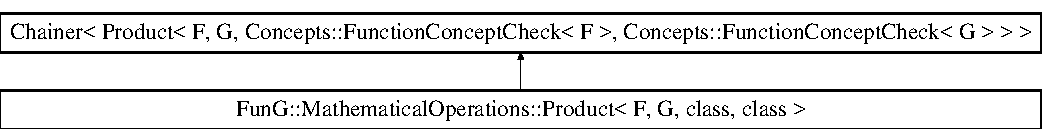
\includegraphics[height=0.864197cm]{structFunG_1_1MathematicalOperations_1_1Product}
\end{center}
\end{figure}
\subsection*{Public Member Functions}
\begin{DoxyCompactItemize}
\item 
{\footnotesize template$<$class Init\+F , class Init\+G $>$ }\\\hyperlink{structFunG_1_1MathematicalOperations_1_1Product_a98d62512443b8c9d31466998b0fa6ee8}{Product} (const Init\+F \&f\+\_\+, const Init\+G \&g\+\_\+)
\begin{DoxyCompactList}\small\item\em Constructor passing arguments to function constructors. \end{DoxyCompactList}\item 
{\footnotesize template$<$class Arg $>$ }\\void \hyperlink{structFunG_1_1MathematicalOperations_1_1Product_a5b45c1bac06651ee5b6ea79fb5128ef9}{update} (Arg const \&x)
\begin{DoxyCompactList}\small\item\em Update point of evaluation. \end{DoxyCompactList}\item 
{\footnotesize template$<$int index, class Arg $>$ }\\void \hyperlink{structFunG_1_1MathematicalOperations_1_1Product_a8db3d935bbe273c0436ff3bc6bb6b786}{update} (const Arg \&x)
\begin{DoxyCompactList}\small\item\em Update variable corresponding to index. \end{DoxyCompactList}\item 
auto \hyperlink{structFunG_1_1MathematicalOperations_1_1Product_ad0c816f33a344bc7ca816dbaad9c78f8}{d0} () const noexcept
\begin{DoxyCompactList}\small\item\em Function value. \end{DoxyCompactList}\item 
{\footnotesize template$<$int id, class Arg , class Indexed\+Arg  = Indexed\+Type$<$\+Arg,id$>$, class  = std\+::enable\+\_\+if\+\_\+t$<$ D1\+Type$<$\+Indexed\+Arg$>$\+::present $>$$>$ }\\auto \hyperlink{structFunG_1_1MathematicalOperations_1_1Product_aea69feaac16f79717a85d7b089a80f8f}{d1} (Arg const \&dx) const 
\begin{DoxyCompactList}\small\item\em First directional derivative. \end{DoxyCompactList}\item 
{\footnotesize template$<$int idx, int idy, class Arg\+X , class Arg\+Y , class Indexed\+Arg\+X  = Indexed\+Type$<$\+Arg\+X,idx$>$, class Indexed\+Arg\+Y  = Indexed\+Type$<$\+Arg\+Y,idy$>$, class  = std\+::enable\+\_\+if\+\_\+t$<$ D2\+Type$<$\+Indexed\+Arg\+X,\+Indexed\+Arg\+Y$>$\+::present $>$$>$ }\\auto \hyperlink{structFunG_1_1MathematicalOperations_1_1Product_a91802ff95963324b5f36016ac5f8c5e0}{d2} (Arg\+X const \&dx, Arg\+Y const \&dy) const 
\begin{DoxyCompactList}\small\item\em Second directional derivative. \end{DoxyCompactList}\item 
{\footnotesize template$<$int idx, int idy, int idz, class Arg\+X , class Arg\+Y , class Arg\+Z , class Indexed\+Arg\+X  = Indexed\+Type$<$\+Arg\+X,idx$>$, class Indexed\+Arg\+Y  = Indexed\+Type$<$\+Arg\+Y,idy$>$, class Indexed\+Arg\+Z  = Indexed\+Type$<$\+Arg\+Z,idz$>$, class  = std\+::enable\+\_\+if\+\_\+t$<$ D3\+Type$<$\+Indexed\+Arg\+X,\+Indexed\+Arg\+Y,\+Indexed\+Arg\+Z$>$\+::present $>$$>$ }\\auto \hyperlink{structFunG_1_1MathematicalOperations_1_1Product_a1ba58e174ea3864a63a4158b95fc8db0}{d3} (Arg\+X const \&dx, Arg\+Y const \&dy, Arg\+Z const \&dz) const 
\begin{DoxyCompactList}\small\item\em Third directional derivative. \end{DoxyCompactList}\end{DoxyCompactItemize}


\subsection{Detailed Description}
\subsubsection*{template$<$class F, class G, class = Concepts\+::\+Function\+Concept\+Check$<$\+F$>$, class = Concepts\+::\+Function\+Concept\+Check$<$\+G$>$$>$struct Fun\+G\+::\+Mathematical\+Operations\+::\+Product$<$ F, G, class, class $>$}

Product $fg$ of functions of type F and G (F and G must satisfy the requirements of \hyperlink{structFunG_1_1Concepts_1_1FunctionConcept}{Concepts\+::\+Function\+Concept}). 

\subsection{Constructor \& Destructor Documentation}
\hypertarget{structFunG_1_1MathematicalOperations_1_1Product_a98d62512443b8c9d31466998b0fa6ee8}{}\index{Fun\+G\+::\+Mathematical\+Operations\+::\+Product@{Fun\+G\+::\+Mathematical\+Operations\+::\+Product}!Product@{Product}}
\index{Product@{Product}!Fun\+G\+::\+Mathematical\+Operations\+::\+Product@{Fun\+G\+::\+Mathematical\+Operations\+::\+Product}}
\subsubsection[{Product}]{\setlength{\rightskip}{0pt plus 5cm}template$<$class F , class G , class  = Concepts\+::\+Function\+Concept\+Check$<$\+F$>$, class  = Concepts\+::\+Function\+Concept\+Check$<$\+G$>$$>$ template$<$class Init\+F , class Init\+G $>$ {\bf Fun\+G\+::\+Mathematical\+Operations\+::\+Product}$<$ F, G, class, class $>$\+::{\bf Product} (
\begin{DoxyParamCaption}
\item[{const Init\+F \&}]{f\+\_\+, }
\item[{const Init\+G \&}]{g\+\_\+}
\end{DoxyParamCaption}
)\hspace{0.3cm}{\ttfamily [inline]}}\label{structFunG_1_1MathematicalOperations_1_1Product_a98d62512443b8c9d31466998b0fa6ee8}


Constructor passing arguments to function constructors. 


\begin{DoxyParams}{Parameters}
{\em f\+\_\+} & input for constructor of left side of product \\
\hline
{\em g\+\_\+} & input for constructor of right side of product \\
\hline
\end{DoxyParams}


\subsection{Member Function Documentation}
\hypertarget{structFunG_1_1MathematicalOperations_1_1Product_ad0c816f33a344bc7ca816dbaad9c78f8}{}\index{Fun\+G\+::\+Mathematical\+Operations\+::\+Product@{Fun\+G\+::\+Mathematical\+Operations\+::\+Product}!d0@{d0}}
\index{d0@{d0}!Fun\+G\+::\+Mathematical\+Operations\+::\+Product@{Fun\+G\+::\+Mathematical\+Operations\+::\+Product}}
\subsubsection[{d0}]{\setlength{\rightskip}{0pt plus 5cm}template$<$class F , class G , class  = Concepts\+::\+Function\+Concept\+Check$<$\+F$>$, class  = Concepts\+::\+Function\+Concept\+Check$<$\+G$>$$>$ auto {\bf Fun\+G\+::\+Mathematical\+Operations\+::\+Product}$<$ F, G, class, class $>$\+::d0 (
\begin{DoxyParamCaption}
{}
\end{DoxyParamCaption}
) const\hspace{0.3cm}{\ttfamily [inline]}, {\ttfamily [noexcept]}}\label{structFunG_1_1MathematicalOperations_1_1Product_ad0c816f33a344bc7ca816dbaad9c78f8}


Function value. 

\hypertarget{structFunG_1_1MathematicalOperations_1_1Product_aea69feaac16f79717a85d7b089a80f8f}{}\index{Fun\+G\+::\+Mathematical\+Operations\+::\+Product@{Fun\+G\+::\+Mathematical\+Operations\+::\+Product}!d1@{d1}}
\index{d1@{d1}!Fun\+G\+::\+Mathematical\+Operations\+::\+Product@{Fun\+G\+::\+Mathematical\+Operations\+::\+Product}}
\subsubsection[{d1}]{\setlength{\rightskip}{0pt plus 5cm}template$<$class F , class G , class  = Concepts\+::\+Function\+Concept\+Check$<$\+F$>$, class  = Concepts\+::\+Function\+Concept\+Check$<$\+G$>$$>$ template$<$int id, class Arg , class Indexed\+Arg  = Indexed\+Type$<$\+Arg,id$>$, class  = std\+::enable\+\_\+if\+\_\+t$<$ D1\+Type$<$\+Indexed\+Arg$>$\+::present $>$$>$ auto {\bf Fun\+G\+::\+Mathematical\+Operations\+::\+Product}$<$ F, G, class, class $>$\+::d1 (
\begin{DoxyParamCaption}
\item[{Arg const \&}]{dx}
\end{DoxyParamCaption}
) const\hspace{0.3cm}{\ttfamily [inline]}}\label{structFunG_1_1MathematicalOperations_1_1Product_aea69feaac16f79717a85d7b089a80f8f}


First directional derivative. 


\begin{DoxyParams}{Parameters}
{\em dx} & direction for which the derivative is computed \\
\hline
\end{DoxyParams}
\hypertarget{structFunG_1_1MathematicalOperations_1_1Product_a91802ff95963324b5f36016ac5f8c5e0}{}\index{Fun\+G\+::\+Mathematical\+Operations\+::\+Product@{Fun\+G\+::\+Mathematical\+Operations\+::\+Product}!d2@{d2}}
\index{d2@{d2}!Fun\+G\+::\+Mathematical\+Operations\+::\+Product@{Fun\+G\+::\+Mathematical\+Operations\+::\+Product}}
\subsubsection[{d2}]{\setlength{\rightskip}{0pt plus 5cm}template$<$class F , class G , class  = Concepts\+::\+Function\+Concept\+Check$<$\+F$>$, class  = Concepts\+::\+Function\+Concept\+Check$<$\+G$>$$>$ template$<$int idx, int idy, class Arg\+X , class Arg\+Y , class Indexed\+Arg\+X  = Indexed\+Type$<$\+Arg\+X,idx$>$, class Indexed\+Arg\+Y  = Indexed\+Type$<$\+Arg\+Y,idy$>$, class  = std\+::enable\+\_\+if\+\_\+t$<$ D2\+Type$<$\+Indexed\+Arg\+X,\+Indexed\+Arg\+Y$>$\+::present $>$$>$ auto {\bf Fun\+G\+::\+Mathematical\+Operations\+::\+Product}$<$ F, G, class, class $>$\+::d2 (
\begin{DoxyParamCaption}
\item[{Arg\+X const \&}]{dx, }
\item[{Arg\+Y const \&}]{dy}
\end{DoxyParamCaption}
) const\hspace{0.3cm}{\ttfamily [inline]}}\label{structFunG_1_1MathematicalOperations_1_1Product_a91802ff95963324b5f36016ac5f8c5e0}


Second directional derivative. 


\begin{DoxyParams}{Parameters}
{\em dx} & direction for which the derivative is computed \\
\hline
{\em dy} & direction for which the derivative is computed \\
\hline
\end{DoxyParams}
\hypertarget{structFunG_1_1MathematicalOperations_1_1Product_a1ba58e174ea3864a63a4158b95fc8db0}{}\index{Fun\+G\+::\+Mathematical\+Operations\+::\+Product@{Fun\+G\+::\+Mathematical\+Operations\+::\+Product}!d3@{d3}}
\index{d3@{d3}!Fun\+G\+::\+Mathematical\+Operations\+::\+Product@{Fun\+G\+::\+Mathematical\+Operations\+::\+Product}}
\subsubsection[{d3}]{\setlength{\rightskip}{0pt plus 5cm}template$<$class F , class G , class  = Concepts\+::\+Function\+Concept\+Check$<$\+F$>$, class  = Concepts\+::\+Function\+Concept\+Check$<$\+G$>$$>$ template$<$int idx, int idy, int idz, class Arg\+X , class Arg\+Y , class Arg\+Z , class Indexed\+Arg\+X  = Indexed\+Type$<$\+Arg\+X,idx$>$, class Indexed\+Arg\+Y  = Indexed\+Type$<$\+Arg\+Y,idy$>$, class Indexed\+Arg\+Z  = Indexed\+Type$<$\+Arg\+Z,idz$>$, class  = std\+::enable\+\_\+if\+\_\+t$<$ D3\+Type$<$\+Indexed\+Arg\+X,\+Indexed\+Arg\+Y,\+Indexed\+Arg\+Z$>$\+::present $>$$>$ auto {\bf Fun\+G\+::\+Mathematical\+Operations\+::\+Product}$<$ F, G, class, class $>$\+::d3 (
\begin{DoxyParamCaption}
\item[{Arg\+X const \&}]{dx, }
\item[{Arg\+Y const \&}]{dy, }
\item[{Arg\+Z const \&}]{dz}
\end{DoxyParamCaption}
) const\hspace{0.3cm}{\ttfamily [inline]}}\label{structFunG_1_1MathematicalOperations_1_1Product_a1ba58e174ea3864a63a4158b95fc8db0}


Third directional derivative. 


\begin{DoxyParams}{Parameters}
{\em dx} & direction for which the derivative is computed \\
\hline
{\em dy} & direction for which the derivative is computed \\
\hline
{\em dz} & direction for which the derivative is computed \\
\hline
\end{DoxyParams}
\hypertarget{structFunG_1_1MathematicalOperations_1_1Product_a5b45c1bac06651ee5b6ea79fb5128ef9}{}\index{Fun\+G\+::\+Mathematical\+Operations\+::\+Product@{Fun\+G\+::\+Mathematical\+Operations\+::\+Product}!update@{update}}
\index{update@{update}!Fun\+G\+::\+Mathematical\+Operations\+::\+Product@{Fun\+G\+::\+Mathematical\+Operations\+::\+Product}}
\subsubsection[{update}]{\setlength{\rightskip}{0pt plus 5cm}template$<$class F , class G , class  = Concepts\+::\+Function\+Concept\+Check$<$\+F$>$, class  = Concepts\+::\+Function\+Concept\+Check$<$\+G$>$$>$ template$<$class Arg $>$ void {\bf Fun\+G\+::\+Mathematical\+Operations\+::\+Product}$<$ F, G, class, class $>$\+::update (
\begin{DoxyParamCaption}
\item[{Arg const \&}]{x}
\end{DoxyParamCaption}
)\hspace{0.3cm}{\ttfamily [inline]}}\label{structFunG_1_1MathematicalOperations_1_1Product_a5b45c1bac06651ee5b6ea79fb5128ef9}


Update point of evaluation. 

\hypertarget{structFunG_1_1MathematicalOperations_1_1Product_a8db3d935bbe273c0436ff3bc6bb6b786}{}\index{Fun\+G\+::\+Mathematical\+Operations\+::\+Product@{Fun\+G\+::\+Mathematical\+Operations\+::\+Product}!update@{update}}
\index{update@{update}!Fun\+G\+::\+Mathematical\+Operations\+::\+Product@{Fun\+G\+::\+Mathematical\+Operations\+::\+Product}}
\subsubsection[{update}]{\setlength{\rightskip}{0pt plus 5cm}template$<$class F , class G , class  = Concepts\+::\+Function\+Concept\+Check$<$\+F$>$, class  = Concepts\+::\+Function\+Concept\+Check$<$\+G$>$$>$ template$<$int index, class Arg $>$ void {\bf Fun\+G\+::\+Mathematical\+Operations\+::\+Product}$<$ F, G, class, class $>$\+::update (
\begin{DoxyParamCaption}
\item[{const Arg \&}]{x}
\end{DoxyParamCaption}
)\hspace{0.3cm}{\ttfamily [inline]}}\label{structFunG_1_1MathematicalOperations_1_1Product_a8db3d935bbe273c0436ff3bc6bb6b786}


Update variable corresponding to index. 



The documentation for this struct was generated from the following file\+:\begin{DoxyCompactItemize}
\item 
fung/mathematical\+\_\+operations/\hyperlink{product_8hh}{product.\+hh}\end{DoxyCompactItemize}

\hypertarget{classFunG_1_1LinearAlgebra_1_1RightCauchyGreenStrainTensor}{\section{Fun\-G\-:\-:Linear\-Algebra\-:\-:Right\-Cauchy\-Green\-Strain\-Tensor$<$ Matrix, class $>$ Class Template Reference}
\label{classFunG_1_1LinearAlgebra_1_1RightCauchyGreenStrainTensor}\index{Fun\-G\-::\-Linear\-Algebra\-::\-Right\-Cauchy\-Green\-Strain\-Tensor$<$ Matrix, class $>$@{Fun\-G\-::\-Linear\-Algebra\-::\-Right\-Cauchy\-Green\-Strain\-Tensor$<$ Matrix, class $>$}}
}


Right Cauchy-\/\-Green strain tensor $ F^T F $ for a symmetric matrix $ F $.  




{\ttfamily \#include $<$strain\-\_\-tensor.\-hh$>$}

Inheritance diagram for Fun\-G\-:\-:Linear\-Algebra\-:\-:Right\-Cauchy\-Green\-Strain\-Tensor$<$ Matrix, class $>$\-:\begin{figure}[H]
\begin{center}
\leavevmode
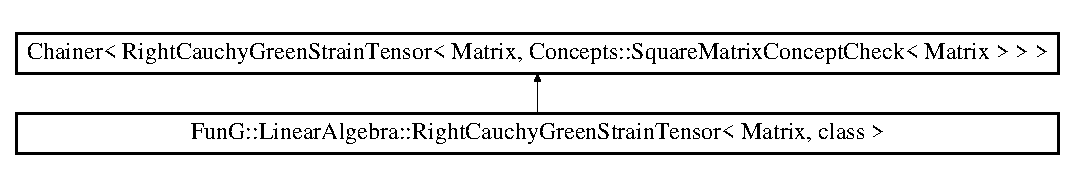
\includegraphics[height=1.830065cm]{classFunG_1_1LinearAlgebra_1_1RightCauchyGreenStrainTensor}
\end{center}
\end{figure}
\subsection*{Public Member Functions}
\begin{DoxyCompactItemize}
\item 
\hyperlink{classFunG_1_1LinearAlgebra_1_1RightCauchyGreenStrainTensor_af4296e26f0ac49f276c06b87522dd0bf}{Right\-Cauchy\-Green\-Strain\-Tensor} ()=default
\item 
\hyperlink{classFunG_1_1LinearAlgebra_1_1RightCauchyGreenStrainTensor_af6085878319f95c8dbe40a6b0de17eb1}{Right\-Cauchy\-Green\-Strain\-Tensor} (const Matrix \&F)
\begin{DoxyCompactList}\small\item\em Constructor. \end{DoxyCompactList}\item 
void \hyperlink{classFunG_1_1LinearAlgebra_1_1RightCauchyGreenStrainTensor_a4517ded8eaf56f040f415b8776dd64a8}{update} (const Matrix \&F)
\begin{DoxyCompactList}\small\item\em Reset point of evaluation. \end{DoxyCompactList}\item 
const Matrix \& \hyperlink{classFunG_1_1LinearAlgebra_1_1RightCauchyGreenStrainTensor_a237357e50d543196ed0228588e911665}{d0} () const noexcept
\begin{DoxyCompactList}\small\item\em Function value $ F^T * F $. \end{DoxyCompactList}\item 
Matrix \hyperlink{classFunG_1_1LinearAlgebra_1_1RightCauchyGreenStrainTensor_ae8746d06ba0d2a127f7775b03d0890a7}{d1} (const Matrix \&d\-F1) const 
\begin{DoxyCompactList}\small\item\em First directional derivative $ F^T dF_1 + dF_1^T F $. \end{DoxyCompactList}\item 
Matrix \hyperlink{classFunG_1_1LinearAlgebra_1_1RightCauchyGreenStrainTensor_a9244629a9ae616c0938e95fbdf68a7d5}{d2} (const Matrix \&d\-F1, const Matrix \&d\-F2) const 
\begin{DoxyCompactList}\small\item\em Second directional derivative $ dF_2^T dF_1 + dF_1^T dF_2 $. \end{DoxyCompactList}\end{DoxyCompactItemize}


\subsection{Detailed Description}
\subsubsection*{template$<$class Matrix, class = Concepts\-::\-Square\-Matrix\-Concept\-Check$<$\-Matrix$>$$>$class Fun\-G\-::\-Linear\-Algebra\-::\-Right\-Cauchy\-Green\-Strain\-Tensor$<$ Matrix, class $>$}

Right Cauchy-\/\-Green strain tensor $ F^T F $ for a symmetric matrix $ F $. 

Used in nonlinear material models based on the deformation gradient $\nabla\varphi$, which takes the role of $F$. 

\subsection{Constructor \& Destructor Documentation}
\hypertarget{classFunG_1_1LinearAlgebra_1_1RightCauchyGreenStrainTensor_af4296e26f0ac49f276c06b87522dd0bf}{\index{Fun\-G\-::\-Linear\-Algebra\-::\-Right\-Cauchy\-Green\-Strain\-Tensor@{Fun\-G\-::\-Linear\-Algebra\-::\-Right\-Cauchy\-Green\-Strain\-Tensor}!Right\-Cauchy\-Green\-Strain\-Tensor@{Right\-Cauchy\-Green\-Strain\-Tensor}}
\index{Right\-Cauchy\-Green\-Strain\-Tensor@{Right\-Cauchy\-Green\-Strain\-Tensor}!FunG::LinearAlgebra::RightCauchyGreenStrainTensor@{Fun\-G\-::\-Linear\-Algebra\-::\-Right\-Cauchy\-Green\-Strain\-Tensor}}
\subsubsection[{Right\-Cauchy\-Green\-Strain\-Tensor}]{\setlength{\rightskip}{0pt plus 5cm}template$<$class Matrix , class  = Concepts\-::\-Square\-Matrix\-Concept\-Check$<$\-Matrix$>$$>$ {\bf Fun\-G\-::\-Linear\-Algebra\-::\-Right\-Cauchy\-Green\-Strain\-Tensor}$<$ Matrix, class $>$\-::{\bf Right\-Cauchy\-Green\-Strain\-Tensor} (
\begin{DoxyParamCaption}
{}
\end{DoxyParamCaption}
)\hspace{0.3cm}{\ttfamily [default]}}}\label{classFunG_1_1LinearAlgebra_1_1RightCauchyGreenStrainTensor_af4296e26f0ac49f276c06b87522dd0bf}
\hypertarget{classFunG_1_1LinearAlgebra_1_1RightCauchyGreenStrainTensor_af6085878319f95c8dbe40a6b0de17eb1}{\index{Fun\-G\-::\-Linear\-Algebra\-::\-Right\-Cauchy\-Green\-Strain\-Tensor@{Fun\-G\-::\-Linear\-Algebra\-::\-Right\-Cauchy\-Green\-Strain\-Tensor}!Right\-Cauchy\-Green\-Strain\-Tensor@{Right\-Cauchy\-Green\-Strain\-Tensor}}
\index{Right\-Cauchy\-Green\-Strain\-Tensor@{Right\-Cauchy\-Green\-Strain\-Tensor}!FunG::LinearAlgebra::RightCauchyGreenStrainTensor@{Fun\-G\-::\-Linear\-Algebra\-::\-Right\-Cauchy\-Green\-Strain\-Tensor}}
\subsubsection[{Right\-Cauchy\-Green\-Strain\-Tensor}]{\setlength{\rightskip}{0pt plus 5cm}template$<$class Matrix , class  = Concepts\-::\-Square\-Matrix\-Concept\-Check$<$\-Matrix$>$$>$ {\bf Fun\-G\-::\-Linear\-Algebra\-::\-Right\-Cauchy\-Green\-Strain\-Tensor}$<$ Matrix, class $>$\-::{\bf Right\-Cauchy\-Green\-Strain\-Tensor} (
\begin{DoxyParamCaption}
\item[{const Matrix \&}]{F}
\end{DoxyParamCaption}
)\hspace{0.3cm}{\ttfamily [inline]}, {\ttfamily [explicit]}}}\label{classFunG_1_1LinearAlgebra_1_1RightCauchyGreenStrainTensor_af6085878319f95c8dbe40a6b0de17eb1}


Constructor. 


\begin{DoxyParams}{Parameters}
{\em F} & point of evaluation. \\
\hline
\end{DoxyParams}


\subsection{Member Function Documentation}
\hypertarget{classFunG_1_1LinearAlgebra_1_1RightCauchyGreenStrainTensor_a237357e50d543196ed0228588e911665}{\index{Fun\-G\-::\-Linear\-Algebra\-::\-Right\-Cauchy\-Green\-Strain\-Tensor@{Fun\-G\-::\-Linear\-Algebra\-::\-Right\-Cauchy\-Green\-Strain\-Tensor}!d0@{d0}}
\index{d0@{d0}!FunG::LinearAlgebra::RightCauchyGreenStrainTensor@{Fun\-G\-::\-Linear\-Algebra\-::\-Right\-Cauchy\-Green\-Strain\-Tensor}}
\subsubsection[{d0}]{\setlength{\rightskip}{0pt plus 5cm}template$<$class Matrix , class  = Concepts\-::\-Square\-Matrix\-Concept\-Check$<$\-Matrix$>$$>$ const Matrix\& {\bf Fun\-G\-::\-Linear\-Algebra\-::\-Right\-Cauchy\-Green\-Strain\-Tensor}$<$ Matrix, class $>$\-::d0 (
\begin{DoxyParamCaption}
{}
\end{DoxyParamCaption}
) const\hspace{0.3cm}{\ttfamily [inline]}, {\ttfamily [noexcept]}}}\label{classFunG_1_1LinearAlgebra_1_1RightCauchyGreenStrainTensor_a237357e50d543196ed0228588e911665}


Function value $ F^T * F $. 

\hypertarget{classFunG_1_1LinearAlgebra_1_1RightCauchyGreenStrainTensor_ae8746d06ba0d2a127f7775b03d0890a7}{\index{Fun\-G\-::\-Linear\-Algebra\-::\-Right\-Cauchy\-Green\-Strain\-Tensor@{Fun\-G\-::\-Linear\-Algebra\-::\-Right\-Cauchy\-Green\-Strain\-Tensor}!d1@{d1}}
\index{d1@{d1}!FunG::LinearAlgebra::RightCauchyGreenStrainTensor@{Fun\-G\-::\-Linear\-Algebra\-::\-Right\-Cauchy\-Green\-Strain\-Tensor}}
\subsubsection[{d1}]{\setlength{\rightskip}{0pt plus 5cm}template$<$class Matrix , class  = Concepts\-::\-Square\-Matrix\-Concept\-Check$<$\-Matrix$>$$>$ Matrix {\bf Fun\-G\-::\-Linear\-Algebra\-::\-Right\-Cauchy\-Green\-Strain\-Tensor}$<$ Matrix, class $>$\-::d1 (
\begin{DoxyParamCaption}
\item[{const Matrix \&}]{d\-F1}
\end{DoxyParamCaption}
) const\hspace{0.3cm}{\ttfamily [inline]}}}\label{classFunG_1_1LinearAlgebra_1_1RightCauchyGreenStrainTensor_ae8746d06ba0d2a127f7775b03d0890a7}


First directional derivative $ F^T dF_1 + dF_1^T F $. 

\hypertarget{classFunG_1_1LinearAlgebra_1_1RightCauchyGreenStrainTensor_a9244629a9ae616c0938e95fbdf68a7d5}{\index{Fun\-G\-::\-Linear\-Algebra\-::\-Right\-Cauchy\-Green\-Strain\-Tensor@{Fun\-G\-::\-Linear\-Algebra\-::\-Right\-Cauchy\-Green\-Strain\-Tensor}!d2@{d2}}
\index{d2@{d2}!FunG::LinearAlgebra::RightCauchyGreenStrainTensor@{Fun\-G\-::\-Linear\-Algebra\-::\-Right\-Cauchy\-Green\-Strain\-Tensor}}
\subsubsection[{d2}]{\setlength{\rightskip}{0pt plus 5cm}template$<$class Matrix , class  = Concepts\-::\-Square\-Matrix\-Concept\-Check$<$\-Matrix$>$$>$ Matrix {\bf Fun\-G\-::\-Linear\-Algebra\-::\-Right\-Cauchy\-Green\-Strain\-Tensor}$<$ Matrix, class $>$\-::d2 (
\begin{DoxyParamCaption}
\item[{const Matrix \&}]{d\-F1, }
\item[{const Matrix \&}]{d\-F2}
\end{DoxyParamCaption}
) const\hspace{0.3cm}{\ttfamily [inline]}}}\label{classFunG_1_1LinearAlgebra_1_1RightCauchyGreenStrainTensor_a9244629a9ae616c0938e95fbdf68a7d5}


Second directional derivative $ dF_2^T dF_1 + dF_1^T dF_2 $. 

\hypertarget{classFunG_1_1LinearAlgebra_1_1RightCauchyGreenStrainTensor_a4517ded8eaf56f040f415b8776dd64a8}{\index{Fun\-G\-::\-Linear\-Algebra\-::\-Right\-Cauchy\-Green\-Strain\-Tensor@{Fun\-G\-::\-Linear\-Algebra\-::\-Right\-Cauchy\-Green\-Strain\-Tensor}!update@{update}}
\index{update@{update}!FunG::LinearAlgebra::RightCauchyGreenStrainTensor@{Fun\-G\-::\-Linear\-Algebra\-::\-Right\-Cauchy\-Green\-Strain\-Tensor}}
\subsubsection[{update}]{\setlength{\rightskip}{0pt plus 5cm}template$<$class Matrix , class  = Concepts\-::\-Square\-Matrix\-Concept\-Check$<$\-Matrix$>$$>$ void {\bf Fun\-G\-::\-Linear\-Algebra\-::\-Right\-Cauchy\-Green\-Strain\-Tensor}$<$ Matrix, class $>$\-::update (
\begin{DoxyParamCaption}
\item[{const Matrix \&}]{F}
\end{DoxyParamCaption}
)\hspace{0.3cm}{\ttfamily [inline]}}}\label{classFunG_1_1LinearAlgebra_1_1RightCauchyGreenStrainTensor_a4517ded8eaf56f040f415b8776dd64a8}


Reset point of evaluation. 



The documentation for this class was generated from the following file\-:\begin{DoxyCompactItemize}
\item 
fung/linear\-\_\-algebra/\hyperlink{strain__tensor_8hh}{strain\-\_\-tensor.\-hh}\end{DoxyCompactItemize}

\hypertarget{structFunG_1_1MathematicalOperations_1_1Scale}{\section{Fun\-G\-:\-:Mathematical\-Operations\-:\-:Scale$<$ F, class $>$ Struct Template Reference}
\label{structFunG_1_1MathematicalOperations_1_1Scale}\index{Fun\-G\-::\-Mathematical\-Operations\-::\-Scale$<$ F, class $>$@{Fun\-G\-::\-Mathematical\-Operations\-::\-Scale$<$ F, class $>$}}
}


Scaling $ af $ of some function $ f $ with a double $ a $ (F must satisfy the requirements of \hyperlink{structFunG_1_1Concepts_1_1FunctionConcept}{Concepts\-::\-Function\-Concept}).  




{\ttfamily \#include $<$scale.\-hh$>$}

Inheritance diagram for Fun\-G\-:\-:Mathematical\-Operations\-:\-:Scale$<$ F, class $>$\-:\begin{figure}[H]
\begin{center}
\leavevmode
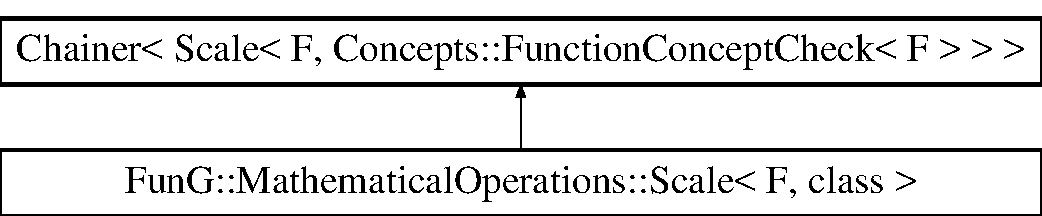
\includegraphics[height=1.717791cm]{structFunG_1_1MathematicalOperations_1_1Scale}
\end{center}
\end{figure}
\subsection*{Public Member Functions}
\begin{DoxyCompactItemize}
\item 
\hypertarget{structFunG_1_1MathematicalOperations_1_1Scale_a8a1c804cb79b41f4e6df28d1e6fe1b72}{\hyperlink{structFunG_1_1MathematicalOperations_1_1Scale_a8a1c804cb79b41f4e6df28d1e6fe1b72}{Scale} ()=default}\label{structFunG_1_1MathematicalOperations_1_1Scale_a8a1c804cb79b41f4e6df28d1e6fe1b72}

\begin{DoxyCompactList}\small\item\em Default constructor. May leave member variables uninitialized! Call update before using evaluation. \end{DoxyCompactList}\item 
{\footnotesize template$<$class Init\-F $>$ }\\\hyperlink{structFunG_1_1MathematicalOperations_1_1Scale_ab86612b868aaee66786793da2ec7a54a}{Scale} (double a\-\_\-, const Init\-F \&f\-\_\-)
\begin{DoxyCompactList}\small\item\em Constructor passing arguments to function constructor. \end{DoxyCompactList}\item 
\hypertarget{structFunG_1_1MathematicalOperations_1_1Scale_adf33e493258919142e39bcb9d27dafd2}{{\footnotesize template$<$class Arg $>$ }\\void \hyperlink{structFunG_1_1MathematicalOperations_1_1Scale_adf33e493258919142e39bcb9d27dafd2}{update} (Arg const \&arg)}\label{structFunG_1_1MathematicalOperations_1_1Scale_adf33e493258919142e39bcb9d27dafd2}

\begin{DoxyCompactList}\small\item\em Reset point of evaluation. \end{DoxyCompactList}\item 
\hypertarget{structFunG_1_1MathematicalOperations_1_1Scale_a5241be9984371f5cf5890d670ae6ed93}{{\footnotesize template$<$int index, class Arg $>$ }\\void \hyperlink{structFunG_1_1MathematicalOperations_1_1Scale_a5241be9984371f5cf5890d670ae6ed93}{update\-Variable} (const Arg \&x)}\label{structFunG_1_1MathematicalOperations_1_1Scale_a5241be9984371f5cf5890d670ae6ed93}

\begin{DoxyCompactList}\small\item\em Propagate call to \hyperlink{structFunG_1_1MathematicalOperations_1_1Scale_a5241be9984371f5cf5890d670ae6ed93}{update\-Variable()} to f. \end{DoxyCompactList}\item 
\hypertarget{structFunG_1_1MathematicalOperations_1_1Scale_ae49c1126f8dbc9d3b03e6890392b86ea}{const auto \& \hyperlink{structFunG_1_1MathematicalOperations_1_1Scale_ae49c1126f8dbc9d3b03e6890392b86ea}{d0} () const noexcept}\label{structFunG_1_1MathematicalOperations_1_1Scale_ae49c1126f8dbc9d3b03e6890392b86ea}

\begin{DoxyCompactList}\small\item\em Function value. \end{DoxyCompactList}\item 
{\footnotesize template$<$int idx, class Arg , class Indexed\-Arg  = Indexed\-Type$<$\-Arg,idx$>$, class  = std\-::enable\-\_\-if\-\_\-t$<$ D1$<$\-F,\-Indexed\-Arg$>$\-::present$>$$>$ }\\auto \hyperlink{structFunG_1_1MathematicalOperations_1_1Scale_a63b6f3353439de0125836020bd2b15ba}{d1} (Arg const \&dx) const 
\begin{DoxyCompactList}\small\item\em First directional derivative. \end{DoxyCompactList}\item 
{\footnotesize template$<$int idx, int idy, class Arg\-X , class Arg\-Y , class Indexed\-Arg\-X  = Indexed\-Type$<$\-Arg\-X,idx$>$, class Indexed\-Arg\-Y  = Indexed\-Type$<$\-Arg\-Y,idy$>$, class  = std\-::enable\-\_\-if\-\_\-t$<$ D2$<$\-F,\-Indexed\-Arg\-X,\-Indexed\-Arg\-Y$>$\-::present$>$$>$ }\\auto \hyperlink{structFunG_1_1MathematicalOperations_1_1Scale_a79be0256e8b2b28c32dbcc9d3c098909}{d2} (Arg\-X const \&dx, Arg\-Y const \&dy) const 
\begin{DoxyCompactList}\small\item\em Second directional derivative. \end{DoxyCompactList}\item 
{\footnotesize template$<$int idx, int idy, int idz, class Arg\-X , class Arg\-Y , class Arg\-Z , class Indexed\-Arg\-X  = Indexed\-Type$<$\-Arg\-X,idx$>$, class Indexed\-Arg\-Y  = Indexed\-Type$<$\-Arg\-Y,idy$>$, class Indexed\-Arg\-Z  = Indexed\-Type$<$\-Arg\-Z,idz$>$, class  = std\-::enable\-\_\-if\-\_\-t$<$ D3$<$\-F,\-Indexed\-Arg\-X,\-Indexed\-Arg\-Y,\-Indexed\-Arg\-Z$>$\-::present $>$$>$ }\\auto \hyperlink{structFunG_1_1MathematicalOperations_1_1Scale_a8cb9d13e8bd87c2d4657ae1c075e7f39}{d3} (Arg\-X const \&dx, Arg\-Y const \&dy, Arg\-Z const \&dz) const 
\begin{DoxyCompactList}\small\item\em Third directional derivative. \end{DoxyCompactList}\end{DoxyCompactItemize}


\subsection{Detailed Description}
\subsubsection*{template$<$class F, class = Function\-Concept\-Check$<$\-F$>$$>$struct Fun\-G\-::\-Mathematical\-Operations\-::\-Scale$<$ F, class $>$}

Scaling $ af $ of some function $ f $ with a double $ a $ (F must satisfy the requirements of \hyperlink{structFunG_1_1Concepts_1_1FunctionConcept}{Concepts\-::\-Function\-Concept}). 

\subsection{Constructor \& Destructor Documentation}
\hypertarget{structFunG_1_1MathematicalOperations_1_1Scale_ab86612b868aaee66786793da2ec7a54a}{\index{Fun\-G\-::\-Mathematical\-Operations\-::\-Scale@{Fun\-G\-::\-Mathematical\-Operations\-::\-Scale}!Scale@{Scale}}
\index{Scale@{Scale}!FunG::MathematicalOperations::Scale@{Fun\-G\-::\-Mathematical\-Operations\-::\-Scale}}
\subsubsection[{Scale}]{\setlength{\rightskip}{0pt plus 5cm}template$<$class F , class  = Function\-Concept\-Check$<$\-F$>$$>$ template$<$class Init\-F $>$ {\bf Fun\-G\-::\-Mathematical\-Operations\-::\-Scale}$<$ F, class $>$\-::{\bf Scale} (
\begin{DoxyParamCaption}
\item[{double}]{a\-\_\-, }
\item[{const Init\-F \&}]{f\-\_\-}
\end{DoxyParamCaption}
)\hspace{0.3cm}{\ttfamily [inline]}}}\label{structFunG_1_1MathematicalOperations_1_1Scale_ab86612b868aaee66786793da2ec7a54a}


Constructor passing arguments to function constructor. 


\begin{DoxyParams}{Parameters}
{\em a\-\_\-} & scaling \\
\hline
{\em f\-\_\-} & input for constructor of outer function \\
\hline
\end{DoxyParams}


\subsection{Member Function Documentation}
\hypertarget{structFunG_1_1MathematicalOperations_1_1Scale_a63b6f3353439de0125836020bd2b15ba}{\index{Fun\-G\-::\-Mathematical\-Operations\-::\-Scale@{Fun\-G\-::\-Mathematical\-Operations\-::\-Scale}!d1@{d1}}
\index{d1@{d1}!FunG::MathematicalOperations::Scale@{Fun\-G\-::\-Mathematical\-Operations\-::\-Scale}}
\subsubsection[{d1}]{\setlength{\rightskip}{0pt plus 5cm}template$<$class F , class  = Function\-Concept\-Check$<$\-F$>$$>$ template$<$int idx, class Arg , class Indexed\-Arg  = Indexed\-Type$<$\-Arg,idx$>$, class  = std\-::enable\-\_\-if\-\_\-t$<$ D1$<$\-F,\-Indexed\-Arg$>$\-::present$>$$>$ auto {\bf Fun\-G\-::\-Mathematical\-Operations\-::\-Scale}$<$ F, class $>$\-::d1 (
\begin{DoxyParamCaption}
\item[{Arg const \&}]{dx}
\end{DoxyParamCaption}
) const\hspace{0.3cm}{\ttfamily [inline]}}}\label{structFunG_1_1MathematicalOperations_1_1Scale_a63b6f3353439de0125836020bd2b15ba}


First directional derivative. 


\begin{DoxyParams}{Parameters}
{\em dx} & direction for which the derivative is computed \\
\hline
\end{DoxyParams}
\hypertarget{structFunG_1_1MathematicalOperations_1_1Scale_a79be0256e8b2b28c32dbcc9d3c098909}{\index{Fun\-G\-::\-Mathematical\-Operations\-::\-Scale@{Fun\-G\-::\-Mathematical\-Operations\-::\-Scale}!d2@{d2}}
\index{d2@{d2}!FunG::MathematicalOperations::Scale@{Fun\-G\-::\-Mathematical\-Operations\-::\-Scale}}
\subsubsection[{d2}]{\setlength{\rightskip}{0pt plus 5cm}template$<$class F , class  = Function\-Concept\-Check$<$\-F$>$$>$ template$<$int idx, int idy, class Arg\-X , class Arg\-Y , class Indexed\-Arg\-X  = Indexed\-Type$<$\-Arg\-X,idx$>$, class Indexed\-Arg\-Y  = Indexed\-Type$<$\-Arg\-Y,idy$>$, class  = std\-::enable\-\_\-if\-\_\-t$<$ D2$<$\-F,\-Indexed\-Arg\-X,\-Indexed\-Arg\-Y$>$\-::present$>$$>$ auto {\bf Fun\-G\-::\-Mathematical\-Operations\-::\-Scale}$<$ F, class $>$\-::d2 (
\begin{DoxyParamCaption}
\item[{Arg\-X const \&}]{dx, }
\item[{Arg\-Y const \&}]{dy}
\end{DoxyParamCaption}
) const\hspace{0.3cm}{\ttfamily [inline]}}}\label{structFunG_1_1MathematicalOperations_1_1Scale_a79be0256e8b2b28c32dbcc9d3c098909}


Second directional derivative. 


\begin{DoxyParams}{Parameters}
{\em dx} & direction for which the derivative is computed \\
\hline
{\em dy} & direction for which the derivative is computed \\
\hline
\end{DoxyParams}
\hypertarget{structFunG_1_1MathematicalOperations_1_1Scale_a8cb9d13e8bd87c2d4657ae1c075e7f39}{\index{Fun\-G\-::\-Mathematical\-Operations\-::\-Scale@{Fun\-G\-::\-Mathematical\-Operations\-::\-Scale}!d3@{d3}}
\index{d3@{d3}!FunG::MathematicalOperations::Scale@{Fun\-G\-::\-Mathematical\-Operations\-::\-Scale}}
\subsubsection[{d3}]{\setlength{\rightskip}{0pt plus 5cm}template$<$class F , class  = Function\-Concept\-Check$<$\-F$>$$>$ template$<$int idx, int idy, int idz, class Arg\-X , class Arg\-Y , class Arg\-Z , class Indexed\-Arg\-X  = Indexed\-Type$<$\-Arg\-X,idx$>$, class Indexed\-Arg\-Y  = Indexed\-Type$<$\-Arg\-Y,idy$>$, class Indexed\-Arg\-Z  = Indexed\-Type$<$\-Arg\-Z,idz$>$, class  = std\-::enable\-\_\-if\-\_\-t$<$ D3$<$\-F,\-Indexed\-Arg\-X,\-Indexed\-Arg\-Y,\-Indexed\-Arg\-Z$>$\-::present $>$$>$ auto {\bf Fun\-G\-::\-Mathematical\-Operations\-::\-Scale}$<$ F, class $>$\-::d3 (
\begin{DoxyParamCaption}
\item[{Arg\-X const \&}]{dx, }
\item[{Arg\-Y const \&}]{dy, }
\item[{Arg\-Z const \&}]{dz}
\end{DoxyParamCaption}
) const\hspace{0.3cm}{\ttfamily [inline]}}}\label{structFunG_1_1MathematicalOperations_1_1Scale_a8cb9d13e8bd87c2d4657ae1c075e7f39}


Third directional derivative. 


\begin{DoxyParams}{Parameters}
{\em dx} & direction for which the derivative is computed \\
\hline
{\em dy} & direction for which the derivative is computed \\
\hline
{\em dz} & direction for which the derivative is computed \\
\hline
\end{DoxyParams}


The documentation for this struct was generated from the following file\-:\begin{DoxyCompactItemize}
\item 
Fun\-G/\-Mathematical\-Operations/scale.\-hh\end{DoxyCompactItemize}

\hypertarget{classFunG_1_1LinearAlgebra_1_1SecondPrincipalInvariant}{}\section{FunG\+:\+:Linear\+Algebra\+:\+:Second\+Principal\+Invariant$<$ Matrix, class $>$ Class Template Reference}
\label{classFunG_1_1LinearAlgebra_1_1SecondPrincipalInvariant}\index{Fun\+G\+::\+Linear\+Algebra\+::\+Second\+Principal\+Invariant$<$ Matrix, class $>$@{Fun\+G\+::\+Linear\+Algebra\+::\+Second\+Principal\+Invariant$<$ Matrix, class $>$}}


Second principal invariant $ \iota_2(A)=\mathrm{tr}(\mathrm{cof}(A)) $ for $A\in\mathbb{R}^{n,n}$.  




{\ttfamily \#include $<$principal\+\_\+invariants.\+hh$>$}

Inheritance diagram for FunG\+:\+:Linear\+Algebra\+:\+:Second\+Principal\+Invariant$<$ Matrix, class $>$\+:\begin{figure}[H]
\begin{center}
\leavevmode
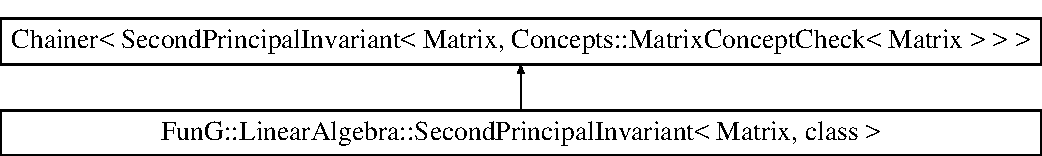
\includegraphics[height=2.000000cm]{classFunG_1_1LinearAlgebra_1_1SecondPrincipalInvariant}
\end{center}
\end{figure}
\subsection*{Public Member Functions}
\begin{DoxyCompactItemize}
\item 
\hyperlink{classFunG_1_1LinearAlgebra_1_1SecondPrincipalInvariant_a959bed7e38dae7003556a582a978cdb1}{Second\+Principal\+Invariant} ()=default
\item 
\hyperlink{classFunG_1_1LinearAlgebra_1_1SecondPrincipalInvariant_ab04cf850a3475333f64e5e4d572d0685}{Second\+Principal\+Invariant} (const Matrix \&A)
\begin{DoxyCompactList}\small\item\em Constructor. \end{DoxyCompactList}\item 
void \hyperlink{classFunG_1_1LinearAlgebra_1_1SecondPrincipalInvariant_a511f6f78f64fc8f1fe9315c8256e285f}{update} (const Matrix \&A)
\begin{DoxyCompactList}\small\item\em Reset matrix to compute second principal invariant from. \end{DoxyCompactList}\item 
auto \hyperlink{classFunG_1_1LinearAlgebra_1_1SecondPrincipalInvariant_af7df9e46d302c070777db975c1161df0}{d0} () const 
\begin{DoxyCompactList}\small\item\em Value of the second principal invariant. \end{DoxyCompactList}\item 
auto \hyperlink{classFunG_1_1LinearAlgebra_1_1SecondPrincipalInvariant_aae55f9cb645def405d16fdbdcc6ccc6b}{d1} (const Matrix \&d\+A1) const 
\begin{DoxyCompactList}\small\item\em First directional derivative. \end{DoxyCompactList}\item 
auto \hyperlink{classFunG_1_1LinearAlgebra_1_1SecondPrincipalInvariant_aa1e9d775263e231afd1a8ba9cdc17963}{d2} (const Matrix \&d\+A1, const Matrix \&d\+A2) const 
\begin{DoxyCompactList}\small\item\em Second directional derivative. \end{DoxyCompactList}\end{DoxyCompactItemize}


\subsection{Detailed Description}
\subsubsection*{template$<$class Matrix, class = Concepts\+::\+Matrix\+Concept\+Check$<$\+Matrix$>$$>$\\*
class Fun\+G\+::\+Linear\+Algebra\+::\+Second\+Principal\+Invariant$<$ Matrix, class $>$}

Second principal invariant $ \iota_2(A)=\mathrm{tr}(\mathrm{cof}(A)) $ for $A\in\mathbb{R}^{n,n}$. 

\subsection{Constructor \& Destructor Documentation}
\index{Fun\+G\+::\+Linear\+Algebra\+::\+Second\+Principal\+Invariant@{Fun\+G\+::\+Linear\+Algebra\+::\+Second\+Principal\+Invariant}!Second\+Principal\+Invariant@{Second\+Principal\+Invariant}}
\index{Second\+Principal\+Invariant@{Second\+Principal\+Invariant}!Fun\+G\+::\+Linear\+Algebra\+::\+Second\+Principal\+Invariant@{Fun\+G\+::\+Linear\+Algebra\+::\+Second\+Principal\+Invariant}}
\subsubsection[{\texorpdfstring{Second\+Principal\+Invariant()=default}{SecondPrincipalInvariant()=default}}]{\setlength{\rightskip}{0pt plus 5cm}template$<$class Matrix, class  = Concepts\+::\+Matrix\+Concept\+Check$<$\+Matrix$>$$>$ {\bf Fun\+G\+::\+Linear\+Algebra\+::\+Second\+Principal\+Invariant}$<$ Matrix, class $>$\+::{\bf Second\+Principal\+Invariant} (
\begin{DoxyParamCaption}
{}
\end{DoxyParamCaption}
)\hspace{0.3cm}{\ttfamily [default]}}\hypertarget{classFunG_1_1LinearAlgebra_1_1SecondPrincipalInvariant_a959bed7e38dae7003556a582a978cdb1}{}\label{classFunG_1_1LinearAlgebra_1_1SecondPrincipalInvariant_a959bed7e38dae7003556a582a978cdb1}
\index{Fun\+G\+::\+Linear\+Algebra\+::\+Second\+Principal\+Invariant@{Fun\+G\+::\+Linear\+Algebra\+::\+Second\+Principal\+Invariant}!Second\+Principal\+Invariant@{Second\+Principal\+Invariant}}
\index{Second\+Principal\+Invariant@{Second\+Principal\+Invariant}!Fun\+G\+::\+Linear\+Algebra\+::\+Second\+Principal\+Invariant@{Fun\+G\+::\+Linear\+Algebra\+::\+Second\+Principal\+Invariant}}
\subsubsection[{\texorpdfstring{Second\+Principal\+Invariant(const Matrix \&\+A)}{SecondPrincipalInvariant(const Matrix &A)}}]{\setlength{\rightskip}{0pt plus 5cm}template$<$class Matrix, class  = Concepts\+::\+Matrix\+Concept\+Check$<$\+Matrix$>$$>$ {\bf Fun\+G\+::\+Linear\+Algebra\+::\+Second\+Principal\+Invariant}$<$ Matrix, class $>$\+::{\bf Second\+Principal\+Invariant} (
\begin{DoxyParamCaption}
\item[{const Matrix \&}]{A}
\end{DoxyParamCaption}
)\hspace{0.3cm}{\ttfamily [inline]}}\hypertarget{classFunG_1_1LinearAlgebra_1_1SecondPrincipalInvariant_ab04cf850a3475333f64e5e4d572d0685}{}\label{classFunG_1_1LinearAlgebra_1_1SecondPrincipalInvariant_ab04cf850a3475333f64e5e4d572d0685}


Constructor. 


\begin{DoxyParams}{Parameters}
{\em A} & matrix to compute second principal invariant from \\
\hline
\end{DoxyParams}


\subsection{Member Function Documentation}
\index{Fun\+G\+::\+Linear\+Algebra\+::\+Second\+Principal\+Invariant@{Fun\+G\+::\+Linear\+Algebra\+::\+Second\+Principal\+Invariant}!d0@{d0}}
\index{d0@{d0}!Fun\+G\+::\+Linear\+Algebra\+::\+Second\+Principal\+Invariant@{Fun\+G\+::\+Linear\+Algebra\+::\+Second\+Principal\+Invariant}}
\subsubsection[{\texorpdfstring{d0() const }{d0() const }}]{\setlength{\rightskip}{0pt plus 5cm}template$<$class Matrix, class  = Concepts\+::\+Matrix\+Concept\+Check$<$\+Matrix$>$$>$ auto {\bf Fun\+G\+::\+Linear\+Algebra\+::\+Second\+Principal\+Invariant}$<$ Matrix, class $>$\+::d0 (
\begin{DoxyParamCaption}
{}
\end{DoxyParamCaption}
) const\hspace{0.3cm}{\ttfamily [inline]}}\hypertarget{classFunG_1_1LinearAlgebra_1_1SecondPrincipalInvariant_af7df9e46d302c070777db975c1161df0}{}\label{classFunG_1_1LinearAlgebra_1_1SecondPrincipalInvariant_af7df9e46d302c070777db975c1161df0}


Value of the second principal invariant. 

\index{Fun\+G\+::\+Linear\+Algebra\+::\+Second\+Principal\+Invariant@{Fun\+G\+::\+Linear\+Algebra\+::\+Second\+Principal\+Invariant}!d1@{d1}}
\index{d1@{d1}!Fun\+G\+::\+Linear\+Algebra\+::\+Second\+Principal\+Invariant@{Fun\+G\+::\+Linear\+Algebra\+::\+Second\+Principal\+Invariant}}
\subsubsection[{\texorpdfstring{d1(const Matrix \&d\+A1) const }{d1(const Matrix &dA1) const }}]{\setlength{\rightskip}{0pt plus 5cm}template$<$class Matrix, class  = Concepts\+::\+Matrix\+Concept\+Check$<$\+Matrix$>$$>$ auto {\bf Fun\+G\+::\+Linear\+Algebra\+::\+Second\+Principal\+Invariant}$<$ Matrix, class $>$\+::d1 (
\begin{DoxyParamCaption}
\item[{const Matrix \&}]{d\+A1}
\end{DoxyParamCaption}
) const\hspace{0.3cm}{\ttfamily [inline]}}\hypertarget{classFunG_1_1LinearAlgebra_1_1SecondPrincipalInvariant_aae55f9cb645def405d16fdbdcc6ccc6b}{}\label{classFunG_1_1LinearAlgebra_1_1SecondPrincipalInvariant_aae55f9cb645def405d16fdbdcc6ccc6b}


First directional derivative. 


\begin{DoxyParams}{Parameters}
{\em d\+A1} & direction for which the derivative is computed \\
\hline
\end{DoxyParams}
\index{Fun\+G\+::\+Linear\+Algebra\+::\+Second\+Principal\+Invariant@{Fun\+G\+::\+Linear\+Algebra\+::\+Second\+Principal\+Invariant}!d2@{d2}}
\index{d2@{d2}!Fun\+G\+::\+Linear\+Algebra\+::\+Second\+Principal\+Invariant@{Fun\+G\+::\+Linear\+Algebra\+::\+Second\+Principal\+Invariant}}
\subsubsection[{\texorpdfstring{d2(const Matrix \&d\+A1, const Matrix \&d\+A2) const }{d2(const Matrix &dA1, const Matrix &dA2) const }}]{\setlength{\rightskip}{0pt plus 5cm}template$<$class Matrix, class  = Concepts\+::\+Matrix\+Concept\+Check$<$\+Matrix$>$$>$ auto {\bf Fun\+G\+::\+Linear\+Algebra\+::\+Second\+Principal\+Invariant}$<$ Matrix, class $>$\+::d2 (
\begin{DoxyParamCaption}
\item[{const Matrix \&}]{d\+A1, }
\item[{const Matrix \&}]{d\+A2}
\end{DoxyParamCaption}
) const\hspace{0.3cm}{\ttfamily [inline]}}\hypertarget{classFunG_1_1LinearAlgebra_1_1SecondPrincipalInvariant_aa1e9d775263e231afd1a8ba9cdc17963}{}\label{classFunG_1_1LinearAlgebra_1_1SecondPrincipalInvariant_aa1e9d775263e231afd1a8ba9cdc17963}


Second directional derivative. 


\begin{DoxyParams}{Parameters}
{\em d\+A1} & direction for which the derivative is computed \\
\hline
{\em d\+A2} & direction for which the derivative is computed \\
\hline
\end{DoxyParams}
\index{Fun\+G\+::\+Linear\+Algebra\+::\+Second\+Principal\+Invariant@{Fun\+G\+::\+Linear\+Algebra\+::\+Second\+Principal\+Invariant}!update@{update}}
\index{update@{update}!Fun\+G\+::\+Linear\+Algebra\+::\+Second\+Principal\+Invariant@{Fun\+G\+::\+Linear\+Algebra\+::\+Second\+Principal\+Invariant}}
\subsubsection[{\texorpdfstring{update(const Matrix \&\+A)}{update(const Matrix &A)}}]{\setlength{\rightskip}{0pt plus 5cm}template$<$class Matrix, class  = Concepts\+::\+Matrix\+Concept\+Check$<$\+Matrix$>$$>$ void {\bf Fun\+G\+::\+Linear\+Algebra\+::\+Second\+Principal\+Invariant}$<$ Matrix, class $>$\+::update (
\begin{DoxyParamCaption}
\item[{const Matrix \&}]{A}
\end{DoxyParamCaption}
)\hspace{0.3cm}{\ttfamily [inline]}}\hypertarget{classFunG_1_1LinearAlgebra_1_1SecondPrincipalInvariant_a511f6f78f64fc8f1fe9315c8256e285f}{}\label{classFunG_1_1LinearAlgebra_1_1SecondPrincipalInvariant_a511f6f78f64fc8f1fe9315c8256e285f}


Reset matrix to compute second principal invariant from. 



The documentation for this class was generated from the following file\+:\begin{DoxyCompactItemize}
\item 
fung/linear\+\_\+algebra/\hyperlink{principal__invariants_8hh}{principal\+\_\+invariants.\+hh}\end{DoxyCompactItemize}

\hypertarget{structFunG_1_1Sin}{}\section{FunG\+:\+:Sin Struct Reference}
\label{structFunG_1_1Sin}\index{Fun\+G\+::\+Sin@{Fun\+G\+::\+Sin}}


Sine function including first three derivatives (based on sin(double) in $<$cmath$>$).  




{\ttfamily \#include $<$sine.\+hh$>$}

Inheritance diagram for FunG\+:\+:Sin\+:\begin{figure}[H]
\begin{center}
\leavevmode
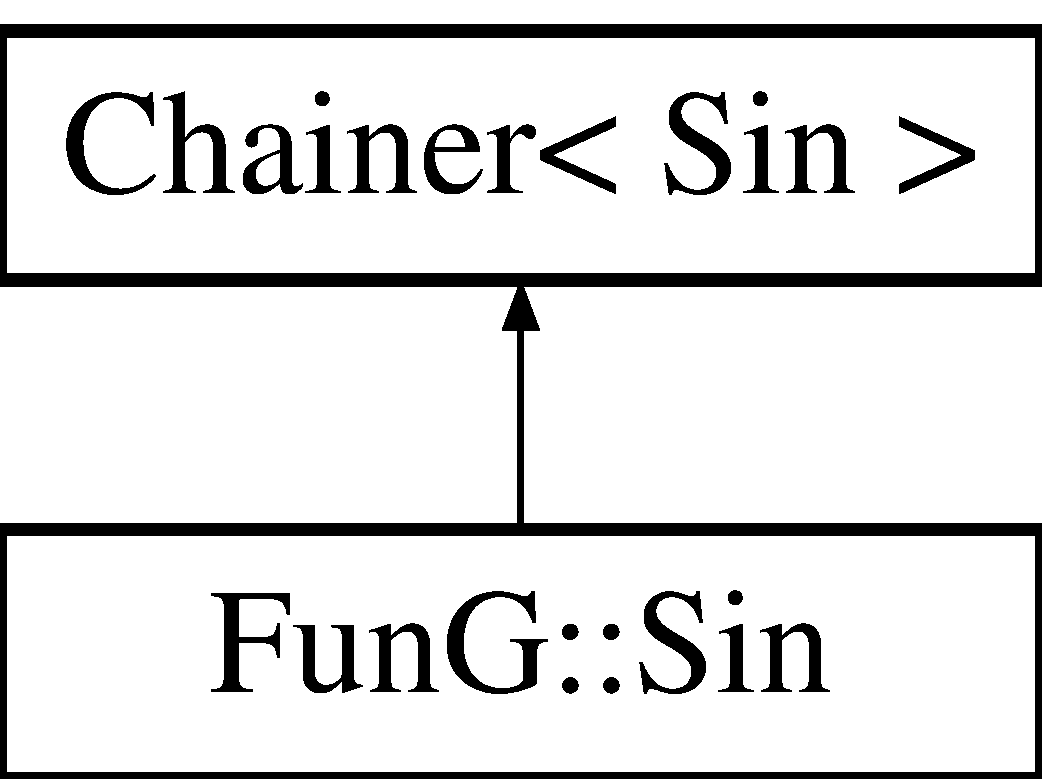
\includegraphics[height=2.000000cm]{structFunG_1_1Sin}
\end{center}
\end{figure}
\subsection*{Public Member Functions}
\begin{DoxyCompactItemize}
\item 
\hyperlink{structFunG_1_1Sin_aa956d10238ebb30a8e037e9f82488a8e}{Sin} (double x=0)
\begin{DoxyCompactList}\small\item\em Constructor. \end{DoxyCompactList}\item 
void \hyperlink{structFunG_1_1Sin_a3f26e1664a29c03e2f29fc2205873850}{update} (double x)
\begin{DoxyCompactList}\small\item\em Set point of evaluation. \end{DoxyCompactList}\item 
double \hyperlink{structFunG_1_1Sin_abae046eecc58398c73f215087460586b}{d0} () const noexcept
\begin{DoxyCompactList}\small\item\em Function value. \end{DoxyCompactList}\item 
double \hyperlink{structFunG_1_1Sin_aaef53b2343e2185e66ec4e9c0319ebdd}{d1} (double dx=1.) const 
\begin{DoxyCompactList}\small\item\em First (directional) derivative. \end{DoxyCompactList}\item 
double \hyperlink{structFunG_1_1Sin_ae0c92547f5da722f0fc642c2ea8f0539}{d2} (double dx=1., double dy=1.) const 
\begin{DoxyCompactList}\small\item\em Second (directional) derivative. \end{DoxyCompactList}\item 
double \hyperlink{structFunG_1_1Sin_a8d8affa45264f36cde9db0bb1464934e}{d3} (double dx=1., double dy=1., double dz=1.) const 
\begin{DoxyCompactList}\small\item\em Third (directional) derivative. \end{DoxyCompactList}\end{DoxyCompactItemize}


\subsection{Detailed Description}
Sine function including first three derivatives (based on sin(double) in $<$cmath$>$). 

For scalar functions directional derivatives are less interesting. Incorporating this function as building block for more complex functions requires directional derivatives. These occur during applications of the chain rule. 

\subsection{Constructor \& Destructor Documentation}
\index{Fun\+G\+::\+Sin@{Fun\+G\+::\+Sin}!Sin@{Sin}}
\index{Sin@{Sin}!Fun\+G\+::\+Sin@{Fun\+G\+::\+Sin}}
\subsubsection[{\texorpdfstring{Sin(double x=0)}{Sin(double x=0)}}]{\setlength{\rightskip}{0pt plus 5cm}Fun\+G\+::\+Sin\+::\+Sin (
\begin{DoxyParamCaption}
\item[{double}]{x = {\ttfamily 0}}
\end{DoxyParamCaption}
)\hspace{0.3cm}{\ttfamily [inline]}, {\ttfamily [explicit]}}\hypertarget{structFunG_1_1Sin_aa956d10238ebb30a8e037e9f82488a8e}{}\label{structFunG_1_1Sin_aa956d10238ebb30a8e037e9f82488a8e}


Constructor. 


\begin{DoxyParams}{Parameters}
{\em x} & point of evaluation \\
\hline
\end{DoxyParams}


\subsection{Member Function Documentation}
\index{Fun\+G\+::\+Sin@{Fun\+G\+::\+Sin}!d0@{d0}}
\index{d0@{d0}!Fun\+G\+::\+Sin@{Fun\+G\+::\+Sin}}
\subsubsection[{\texorpdfstring{d0() const noexcept}{d0() const noexcept}}]{\setlength{\rightskip}{0pt plus 5cm}double Fun\+G\+::\+Sin\+::d0 (
\begin{DoxyParamCaption}
{}
\end{DoxyParamCaption}
) const\hspace{0.3cm}{\ttfamily [inline]}, {\ttfamily [noexcept]}}\hypertarget{structFunG_1_1Sin_abae046eecc58398c73f215087460586b}{}\label{structFunG_1_1Sin_abae046eecc58398c73f215087460586b}


Function value. 

\index{Fun\+G\+::\+Sin@{Fun\+G\+::\+Sin}!d1@{d1}}
\index{d1@{d1}!Fun\+G\+::\+Sin@{Fun\+G\+::\+Sin}}
\subsubsection[{\texorpdfstring{d1(double dx=1.) const }{d1(double dx=1.) const }}]{\setlength{\rightskip}{0pt plus 5cm}double Fun\+G\+::\+Sin\+::d1 (
\begin{DoxyParamCaption}
\item[{double}]{dx = {\ttfamily 1.}}
\end{DoxyParamCaption}
) const\hspace{0.3cm}{\ttfamily [inline]}}\hypertarget{structFunG_1_1Sin_aaef53b2343e2185e66ec4e9c0319ebdd}{}\label{structFunG_1_1Sin_aaef53b2343e2185e66ec4e9c0319ebdd}


First (directional) derivative. 

\index{Fun\+G\+::\+Sin@{Fun\+G\+::\+Sin}!d2@{d2}}
\index{d2@{d2}!Fun\+G\+::\+Sin@{Fun\+G\+::\+Sin}}
\subsubsection[{\texorpdfstring{d2(double dx=1., double dy=1.) const }{d2(double dx=1., double dy=1.) const }}]{\setlength{\rightskip}{0pt plus 5cm}double Fun\+G\+::\+Sin\+::d2 (
\begin{DoxyParamCaption}
\item[{double}]{dx = {\ttfamily 1.}, }
\item[{double}]{dy = {\ttfamily 1.}}
\end{DoxyParamCaption}
) const\hspace{0.3cm}{\ttfamily [inline]}}\hypertarget{structFunG_1_1Sin_ae0c92547f5da722f0fc642c2ea8f0539}{}\label{structFunG_1_1Sin_ae0c92547f5da722f0fc642c2ea8f0539}


Second (directional) derivative. 

\index{Fun\+G\+::\+Sin@{Fun\+G\+::\+Sin}!d3@{d3}}
\index{d3@{d3}!Fun\+G\+::\+Sin@{Fun\+G\+::\+Sin}}
\subsubsection[{\texorpdfstring{d3(double dx=1., double dy=1., double dz=1.) const }{d3(double dx=1., double dy=1., double dz=1.) const }}]{\setlength{\rightskip}{0pt plus 5cm}double Fun\+G\+::\+Sin\+::d3 (
\begin{DoxyParamCaption}
\item[{double}]{dx = {\ttfamily 1.}, }
\item[{double}]{dy = {\ttfamily 1.}, }
\item[{double}]{dz = {\ttfamily 1.}}
\end{DoxyParamCaption}
) const\hspace{0.3cm}{\ttfamily [inline]}}\hypertarget{structFunG_1_1Sin_a8d8affa45264f36cde9db0bb1464934e}{}\label{structFunG_1_1Sin_a8d8affa45264f36cde9db0bb1464934e}


Third (directional) derivative. 

\index{Fun\+G\+::\+Sin@{Fun\+G\+::\+Sin}!update@{update}}
\index{update@{update}!Fun\+G\+::\+Sin@{Fun\+G\+::\+Sin}}
\subsubsection[{\texorpdfstring{update(double x)}{update(double x)}}]{\setlength{\rightskip}{0pt plus 5cm}void Fun\+G\+::\+Sin\+::update (
\begin{DoxyParamCaption}
\item[{double}]{x}
\end{DoxyParamCaption}
)\hspace{0.3cm}{\ttfamily [inline]}}\hypertarget{structFunG_1_1Sin_a3f26e1664a29c03e2f29fc2205873850}{}\label{structFunG_1_1Sin_a3f26e1664a29c03e2f29fc2205873850}


Set point of evaluation. 



The documentation for this struct was generated from the following file\+:\begin{DoxyCompactItemize}
\item 
include/fung/cmath/\hyperlink{sine_8hh}{sine.\+hh}\end{DoxyCompactItemize}

\hypertarget{structFunG_1_1stringify_1_1Sin}{\section{Fun\-G\-:\-:stringify\-:\-:Sin Struct Reference}
\label{structFunG_1_1stringify_1_1Sin}\index{Fun\-G\-::stringify\-::\-Sin@{Fun\-G\-::stringify\-::\-Sin}}
}


{\ttfamily \#include $<$sine.\-hh$>$}

Inheritance diagram for Fun\-G\-:\-:stringify\-:\-:Sin\-:\begin{figure}[H]
\begin{center}
\leavevmode
\includegraphics[height=2.000000cm]{structFunG_1_1stringify_1_1Sin}
\end{center}
\end{figure}
\subsection*{Public Member Functions}
\begin{DoxyCompactItemize}
\item 
\hyperlink{structFunG_1_1stringify_1_1Sin_a18f123f045b466a62e72dd2b6479dd25}{Sin} (\hyperlink{structFunG_1_1String}{String} x=\char`\"{}x\char`\"{})
\begin{DoxyCompactList}\small\item\em Constructor. \end{DoxyCompactList}\item 
void \hyperlink{structFunG_1_1stringify_1_1Sin_a79e51d4a2ed5edd700582ccf13a18fbd}{update} (const \hyperlink{structFunG_1_1String}{String} \&x)
\begin{DoxyCompactList}\small\item\em Set point of evaluation. \end{DoxyCompactList}\item 
\hyperlink{structFunG_1_1String}{String} \hyperlink{structFunG_1_1stringify_1_1Sin_a9b563e01922acc912035e409c839d02c}{d0} () const noexcept
\begin{DoxyCompactList}\small\item\em Function value. \end{DoxyCompactList}\item 
\hyperlink{structFunG_1_1String}{String} \hyperlink{structFunG_1_1stringify_1_1Sin_a3b0f452d7c19c535aaaccd77343c41f9}{d1} (const \hyperlink{structFunG_1_1String}{String} \&dx=\char`\"{}\char`\"{}) const 
\begin{DoxyCompactList}\small\item\em First (directional) derivative. \end{DoxyCompactList}\item 
\hyperlink{structFunG_1_1String}{String} \hyperlink{structFunG_1_1stringify_1_1Sin_a154ea8e43baa2e5711437dbb788f000f}{d2} (const \hyperlink{structFunG_1_1String}{String} \&dx=\char`\"{}\char`\"{}, const \hyperlink{structFunG_1_1String}{String} \&dy=\char`\"{}\char`\"{}) const 
\begin{DoxyCompactList}\small\item\em Second (directional) derivative. \end{DoxyCompactList}\item 
\hyperlink{structFunG_1_1String}{String} \hyperlink{structFunG_1_1stringify_1_1Sin_a66e04eb833fcba2cdbcff7568d57f3c3}{d3} (const \hyperlink{structFunG_1_1String}{String} \&dx=\char`\"{}\char`\"{}, const \hyperlink{structFunG_1_1String}{String} \&dy=\char`\"{}\char`\"{}, const \hyperlink{structFunG_1_1String}{String} \&dz=\char`\"{}\char`\"{}) const 
\begin{DoxyCompactList}\small\item\em Third (directional) derivative. \end{DoxyCompactList}\end{DoxyCompactItemize}


\subsection{Constructor \& Destructor Documentation}
\hypertarget{structFunG_1_1stringify_1_1Sin_a18f123f045b466a62e72dd2b6479dd25}{\index{Fun\-G\-::stringify\-::\-Sin@{Fun\-G\-::stringify\-::\-Sin}!Sin@{Sin}}
\index{Sin@{Sin}!FunG::stringify::Sin@{Fun\-G\-::stringify\-::\-Sin}}
\subsubsection[{Sin}]{\setlength{\rightskip}{0pt plus 5cm}Fun\-G\-::stringify\-::\-Sin\-::\-Sin (
\begin{DoxyParamCaption}
\item[{{\bf String}}]{x = {\ttfamily \char`\"{}x\char`\"{}}}
\end{DoxyParamCaption}
)\hspace{0.3cm}{\ttfamily [inline]}, {\ttfamily [explicit]}}}\label{structFunG_1_1stringify_1_1Sin_a18f123f045b466a62e72dd2b6479dd25}


Constructor. 


\begin{DoxyParams}{Parameters}
{\em x} & point of evaluation \\
\hline
\end{DoxyParams}


\subsection{Member Function Documentation}
\hypertarget{structFunG_1_1stringify_1_1Sin_a9b563e01922acc912035e409c839d02c}{\index{Fun\-G\-::stringify\-::\-Sin@{Fun\-G\-::stringify\-::\-Sin}!d0@{d0}}
\index{d0@{d0}!FunG::stringify::Sin@{Fun\-G\-::stringify\-::\-Sin}}
\subsubsection[{d0}]{\setlength{\rightskip}{0pt plus 5cm}{\bf String} Fun\-G\-::stringify\-::\-Sin\-::d0 (
\begin{DoxyParamCaption}
{}
\end{DoxyParamCaption}
) const\hspace{0.3cm}{\ttfamily [inline]}, {\ttfamily [noexcept]}}}\label{structFunG_1_1stringify_1_1Sin_a9b563e01922acc912035e409c839d02c}


Function value. 

\hypertarget{structFunG_1_1stringify_1_1Sin_a3b0f452d7c19c535aaaccd77343c41f9}{\index{Fun\-G\-::stringify\-::\-Sin@{Fun\-G\-::stringify\-::\-Sin}!d1@{d1}}
\index{d1@{d1}!FunG::stringify::Sin@{Fun\-G\-::stringify\-::\-Sin}}
\subsubsection[{d1}]{\setlength{\rightskip}{0pt plus 5cm}{\bf String} Fun\-G\-::stringify\-::\-Sin\-::d1 (
\begin{DoxyParamCaption}
\item[{const {\bf String} \&}]{dx = {\ttfamily \char`\"{}\char`\"{}}}
\end{DoxyParamCaption}
) const\hspace{0.3cm}{\ttfamily [inline]}}}\label{structFunG_1_1stringify_1_1Sin_a3b0f452d7c19c535aaaccd77343c41f9}


First (directional) derivative. 

\hypertarget{structFunG_1_1stringify_1_1Sin_a154ea8e43baa2e5711437dbb788f000f}{\index{Fun\-G\-::stringify\-::\-Sin@{Fun\-G\-::stringify\-::\-Sin}!d2@{d2}}
\index{d2@{d2}!FunG::stringify::Sin@{Fun\-G\-::stringify\-::\-Sin}}
\subsubsection[{d2}]{\setlength{\rightskip}{0pt plus 5cm}{\bf String} Fun\-G\-::stringify\-::\-Sin\-::d2 (
\begin{DoxyParamCaption}
\item[{const {\bf String} \&}]{dx = {\ttfamily \char`\"{}\char`\"{}}, }
\item[{const {\bf String} \&}]{dy = {\ttfamily \char`\"{}\char`\"{}}}
\end{DoxyParamCaption}
) const\hspace{0.3cm}{\ttfamily [inline]}}}\label{structFunG_1_1stringify_1_1Sin_a154ea8e43baa2e5711437dbb788f000f}


Second (directional) derivative. 

\hypertarget{structFunG_1_1stringify_1_1Sin_a66e04eb833fcba2cdbcff7568d57f3c3}{\index{Fun\-G\-::stringify\-::\-Sin@{Fun\-G\-::stringify\-::\-Sin}!d3@{d3}}
\index{d3@{d3}!FunG::stringify::Sin@{Fun\-G\-::stringify\-::\-Sin}}
\subsubsection[{d3}]{\setlength{\rightskip}{0pt plus 5cm}{\bf String} Fun\-G\-::stringify\-::\-Sin\-::d3 (
\begin{DoxyParamCaption}
\item[{const {\bf String} \&}]{dx = {\ttfamily \char`\"{}\char`\"{}}, }
\item[{const {\bf String} \&}]{dy = {\ttfamily \char`\"{}\char`\"{}}, }
\item[{const {\bf String} \&}]{dz = {\ttfamily \char`\"{}\char`\"{}}}
\end{DoxyParamCaption}
) const\hspace{0.3cm}{\ttfamily [inline]}}}\label{structFunG_1_1stringify_1_1Sin_a66e04eb833fcba2cdbcff7568d57f3c3}


Third (directional) derivative. 

\hypertarget{structFunG_1_1stringify_1_1Sin_a79e51d4a2ed5edd700582ccf13a18fbd}{\index{Fun\-G\-::stringify\-::\-Sin@{Fun\-G\-::stringify\-::\-Sin}!update@{update}}
\index{update@{update}!FunG::stringify::Sin@{Fun\-G\-::stringify\-::\-Sin}}
\subsubsection[{update}]{\setlength{\rightskip}{0pt plus 5cm}void Fun\-G\-::stringify\-::\-Sin\-::update (
\begin{DoxyParamCaption}
\item[{const {\bf String} \&}]{x}
\end{DoxyParamCaption}
)\hspace{0.3cm}{\ttfamily [inline]}}}\label{structFunG_1_1stringify_1_1Sin_a79e51d4a2ed5edd700582ccf13a18fbd}


Set point of evaluation. 



The documentation for this struct was generated from the following file\-:\begin{DoxyCompactItemize}
\item 
include/fung/cmath/stringify/\hyperlink{stringify_2sine_8hh}{sine.\-hh}\end{DoxyCompactItemize}

\hypertarget{structFunG_1_1texify_1_1Sin}{\section{Fun\-G\-:\-:texify\-:\-:Sin Struct Reference}
\label{structFunG_1_1texify_1_1Sin}\index{Fun\-G\-::texify\-::\-Sin@{Fun\-G\-::texify\-::\-Sin}}
}


{\ttfamily \#include $<$sine.\-hh$>$}

Inheritance diagram for Fun\-G\-:\-:texify\-:\-:Sin\-:\begin{figure}[H]
\begin{center}
\leavevmode
\includegraphics[height=2.000000cm]{structFunG_1_1texify_1_1Sin}
\end{center}
\end{figure}
\subsection*{Public Member Functions}
\begin{DoxyCompactItemize}
\item 
\hyperlink{structFunG_1_1texify_1_1Sin_a6001bbfd994aa2a10ec11cf2316c9717}{Sin} (std\-::string x=\char`\"{}x\char`\"{})
\begin{DoxyCompactList}\small\item\em Constructor. \end{DoxyCompactList}\item 
void \hyperlink{structFunG_1_1texify_1_1Sin_ab910ef2ca2b7e27978a4bac16128d703}{update} (const std\-::string \&x)
\begin{DoxyCompactList}\small\item\em Set point of evaluation. \end{DoxyCompactList}\item 
std\-::string \hyperlink{structFunG_1_1texify_1_1Sin_ae2cf01437da9124fc506435a7b88c454}{d0} () const noexcept
\begin{DoxyCompactList}\small\item\em Function value. \end{DoxyCompactList}\item 
std\-::string \hyperlink{structFunG_1_1texify_1_1Sin_abdf4a366a01083db5d3b00d72968932f}{d1} (const std\-::string \&dx=\char`\"{}\char`\"{}) const 
\begin{DoxyCompactList}\small\item\em First (directional) derivative. \end{DoxyCompactList}\item 
std\-::string \hyperlink{structFunG_1_1texify_1_1Sin_a48504a5be408b49e848d958b78f54e90}{d2} (const std\-::string \&dx=\char`\"{}\char`\"{}, const std\-::string \&dy=\char`\"{}\char`\"{}) const 
\begin{DoxyCompactList}\small\item\em Second (directional) derivative. \end{DoxyCompactList}\item 
std\-::string \hyperlink{structFunG_1_1texify_1_1Sin_ac51be9dc4b26ca1bf3df229d826e5ecc}{d3} (const std\-::string \&dx=\char`\"{}\char`\"{}, const std\-::string \&dy=\char`\"{}\char`\"{}, const std\-::string \&dz=\char`\"{}\char`\"{}) const 
\begin{DoxyCompactList}\small\item\em Third (directional) derivative. \end{DoxyCompactList}\end{DoxyCompactItemize}


\subsection{Constructor \& Destructor Documentation}
\hypertarget{structFunG_1_1texify_1_1Sin_a6001bbfd994aa2a10ec11cf2316c9717}{\index{Fun\-G\-::texify\-::\-Sin@{Fun\-G\-::texify\-::\-Sin}!Sin@{Sin}}
\index{Sin@{Sin}!FunG::texify::Sin@{Fun\-G\-::texify\-::\-Sin}}
\subsubsection[{Sin}]{\setlength{\rightskip}{0pt plus 5cm}Fun\-G\-::texify\-::\-Sin\-::\-Sin (
\begin{DoxyParamCaption}
\item[{std\-::string}]{x = {\ttfamily \char`\"{}x\char`\"{}}}
\end{DoxyParamCaption}
)\hspace{0.3cm}{\ttfamily [inline]}, {\ttfamily [explicit]}}}\label{structFunG_1_1texify_1_1Sin_a6001bbfd994aa2a10ec11cf2316c9717}


Constructor. 


\begin{DoxyParams}{Parameters}
{\em x} & point of evaluation \\
\hline
\end{DoxyParams}


\subsection{Member Function Documentation}
\hypertarget{structFunG_1_1texify_1_1Sin_ae2cf01437da9124fc506435a7b88c454}{\index{Fun\-G\-::texify\-::\-Sin@{Fun\-G\-::texify\-::\-Sin}!d0@{d0}}
\index{d0@{d0}!FunG::texify::Sin@{Fun\-G\-::texify\-::\-Sin}}
\subsubsection[{d0}]{\setlength{\rightskip}{0pt plus 5cm}std\-::string Fun\-G\-::texify\-::\-Sin\-::d0 (
\begin{DoxyParamCaption}
{}
\end{DoxyParamCaption}
) const\hspace{0.3cm}{\ttfamily [inline]}, {\ttfamily [noexcept]}}}\label{structFunG_1_1texify_1_1Sin_ae2cf01437da9124fc506435a7b88c454}


Function value. 

\hypertarget{structFunG_1_1texify_1_1Sin_abdf4a366a01083db5d3b00d72968932f}{\index{Fun\-G\-::texify\-::\-Sin@{Fun\-G\-::texify\-::\-Sin}!d1@{d1}}
\index{d1@{d1}!FunG::texify::Sin@{Fun\-G\-::texify\-::\-Sin}}
\subsubsection[{d1}]{\setlength{\rightskip}{0pt plus 5cm}std\-::string Fun\-G\-::texify\-::\-Sin\-::d1 (
\begin{DoxyParamCaption}
\item[{const std\-::string \&}]{dx = {\ttfamily \char`\"{}\char`\"{}}}
\end{DoxyParamCaption}
) const\hspace{0.3cm}{\ttfamily [inline]}}}\label{structFunG_1_1texify_1_1Sin_abdf4a366a01083db5d3b00d72968932f}


First (directional) derivative. 

\hypertarget{structFunG_1_1texify_1_1Sin_a48504a5be408b49e848d958b78f54e90}{\index{Fun\-G\-::texify\-::\-Sin@{Fun\-G\-::texify\-::\-Sin}!d2@{d2}}
\index{d2@{d2}!FunG::texify::Sin@{Fun\-G\-::texify\-::\-Sin}}
\subsubsection[{d2}]{\setlength{\rightskip}{0pt plus 5cm}std\-::string Fun\-G\-::texify\-::\-Sin\-::d2 (
\begin{DoxyParamCaption}
\item[{const std\-::string \&}]{dx = {\ttfamily \char`\"{}\char`\"{}}, }
\item[{const std\-::string \&}]{dy = {\ttfamily \char`\"{}\char`\"{}}}
\end{DoxyParamCaption}
) const\hspace{0.3cm}{\ttfamily [inline]}}}\label{structFunG_1_1texify_1_1Sin_a48504a5be408b49e848d958b78f54e90}


Second (directional) derivative. 

\hypertarget{structFunG_1_1texify_1_1Sin_ac51be9dc4b26ca1bf3df229d826e5ecc}{\index{Fun\-G\-::texify\-::\-Sin@{Fun\-G\-::texify\-::\-Sin}!d3@{d3}}
\index{d3@{d3}!FunG::texify::Sin@{Fun\-G\-::texify\-::\-Sin}}
\subsubsection[{d3}]{\setlength{\rightskip}{0pt plus 5cm}std\-::string Fun\-G\-::texify\-::\-Sin\-::d3 (
\begin{DoxyParamCaption}
\item[{const std\-::string \&}]{dx = {\ttfamily \char`\"{}\char`\"{}}, }
\item[{const std\-::string \&}]{dy = {\ttfamily \char`\"{}\char`\"{}}, }
\item[{const std\-::string \&}]{dz = {\ttfamily \char`\"{}\char`\"{}}}
\end{DoxyParamCaption}
) const\hspace{0.3cm}{\ttfamily [inline]}}}\label{structFunG_1_1texify_1_1Sin_ac51be9dc4b26ca1bf3df229d826e5ecc}


Third (directional) derivative. 

\hypertarget{structFunG_1_1texify_1_1Sin_ab910ef2ca2b7e27978a4bac16128d703}{\index{Fun\-G\-::texify\-::\-Sin@{Fun\-G\-::texify\-::\-Sin}!update@{update}}
\index{update@{update}!FunG::texify::Sin@{Fun\-G\-::texify\-::\-Sin}}
\subsubsection[{update}]{\setlength{\rightskip}{0pt plus 5cm}void Fun\-G\-::texify\-::\-Sin\-::update (
\begin{DoxyParamCaption}
\item[{const std\-::string \&}]{x}
\end{DoxyParamCaption}
)\hspace{0.3cm}{\ttfamily [inline]}}}\label{structFunG_1_1texify_1_1Sin_ab910ef2ca2b7e27978a4bac16128d703}


Set point of evaluation. 



The documentation for this struct was generated from the following file\-:\begin{DoxyCompactItemize}
\item 
include/fung/texify/cmath/\hyperlink{texify_2cmath_2sine_8hh}{sine.\-hh}\end{DoxyCompactItemize}

\hypertarget{structFunG_1_1MathematicalOperations_1_1Squared}{\section{\-Fun\-G\-:\-:\-Mathematical\-Operations\-:\-:\-Squared$<$ \-F, class $>$ \-Struct \-Template \-Reference}
\label{structFunG_1_1MathematicalOperations_1_1Squared}\index{\-Fun\-G\-::\-Mathematical\-Operations\-::\-Squared$<$ F, class $>$@{\-Fun\-G\-::\-Mathematical\-Operations\-::\-Squared$<$ F, class $>$}}
}


\-Squared function $f^2$.  




{\ttfamily \#include $<$squared.\-hh$>$}

\subsection*{\-Public \-Member \-Functions}
\begin{DoxyCompactItemize}
\item 
{\footnotesize template$<$class Init\-F , std\-::enable\-\_\-if\-\_\-t$<$!std\-::is\-\_\-same$<$ std\-::decay\-\_\-t$<$ Init\-F $>$, Squared $>$\-::value $>$ $\ast$  = nullptr$>$ }\\\hyperlink{structFunG_1_1MathematicalOperations_1_1Squared_af786c2153ef17b5d0ddf8e0b51d060d6}{\-Squared} (\-Init\-F \&\&f\-\_\-)
\begin{DoxyCompactList}\small\item\em \-Constructor. \end{DoxyCompactList}\item 
{\footnotesize template$<$class Arg $>$ }\\void \hyperlink{structFunG_1_1MathematicalOperations_1_1Squared_abea95d90dc29ac105c43f4eadde84cab}{update} (\-Arg const \&x)
\begin{DoxyCompactList}\small\item\em \-Update point of evaluation. \end{DoxyCompactList}\item 
{\footnotesize template$<$int index, class Arg $>$ }\\void \hyperlink{structFunG_1_1MathematicalOperations_1_1Squared_a1d890825175df9b79fd73bf8248496ad}{update} (const \-Arg \&x)
\begin{DoxyCompactList}\small\item\em \-Update variable corresponding to index. \end{DoxyCompactList}\item 
\hyperlink{structFunG_1_1MathematicalOperations_1_1Squared_af0560fc3c8a6eed252dfece751a8378d}{decltype} (auto) d0() const noexcept
\begin{DoxyCompactList}\small\item\em \-Function value. \end{DoxyCompactList}\item 
{\footnotesize template$<$int id, class Arg , class Indexed\-Arg  = \-Indexed\-Type$<$\-Arg,id$>$, class  = std\-::enable\-\_\-if\-\_\-t$<$ Compute\-Product$<$ D0$<$\-F$>$ , D1$<$\-F,\-Indexed\-Arg$>$ $>$\-::present $>$$>$ }\\auto \hyperlink{structFunG_1_1MathematicalOperations_1_1Squared_a3fdd893f4a01c7b78f9eba9301d53cce}{d1} (\-Arg const \&dx) const -\/$>$ decay\-\_\-t$<$ \hyperlink{structFunG_1_1MathematicalOperations_1_1Squared_af0560fc3c8a6eed252dfece751a8378d}{decltype}(std
\begin{DoxyCompactList}\small\item\em \-First directional derivative. \end{DoxyCompactList}\item 
{\footnotesize template$<$int idx, int idy, class Arg\-X , class Arg\-Y , class Indexed\-Arg\-X  = \-Indexed\-Type$<$\-Arg\-X,idx$>$, class Indexed\-Arg\-Y  = \-Indexed\-Type$<$\-Arg\-Y,idy$>$, class  = std\-::enable\-\_\-if\-\_\-t$<$ D2\-Sum$<$\-Indexed\-Arg\-X,\-Indexed\-Arg\-Y$>$\-::present $>$$>$ }\\auto \hyperlink{structFunG_1_1MathematicalOperations_1_1Squared_ade05d295a7fd4aa03a2ccd595c03b463}{d2} (\-Arg\-X const \&dx, \-Arg\-Y const \&dy) const -\/$>$ decay\-\_\-t$<$ \hyperlink{structFunG_1_1MathematicalOperations_1_1Squared_af0560fc3c8a6eed252dfece751a8378d}{decltype}(std
\begin{DoxyCompactList}\small\item\em \-Second directional derivative. \end{DoxyCompactList}\item 
{\footnotesize template$<$int idx, int idy, int idz, class Arg\-X , class Arg\-Y , class Arg\-Z , class Indexed\-Arg\-X  = \-Indexed\-Type$<$\-Arg\-X,idx$>$, class Indexed\-Arg\-Y  = \-Indexed\-Type$<$\-Arg\-Y,idy$>$, class Indexed\-Arg\-Z  = \-Indexed\-Type$<$\-Arg\-Z,idz$>$, class  = std\-::enable\-\_\-if\-\_\-t$<$ D3\-Sum$<$\-Indexed\-Arg\-X,\-Indexed\-Arg\-Y,\-Indexed\-Arg\-Z$>$\-::present $>$$>$ }\\auto \hyperlink{structFunG_1_1MathematicalOperations_1_1Squared_a3ead8484cd541d73786747ebca1758e0}{d3} (\-Arg\-X const \&dx, \-Arg\-Y const \&dy, \-Arg\-Z const \&dz) const -\/$>$ decay\-\_\-t$<$ \hyperlink{structFunG_1_1MathematicalOperations_1_1Squared_af0560fc3c8a6eed252dfece751a8378d}{decltype}(std
\begin{DoxyCompactList}\small\item\em \-Third directional derivative. \end{DoxyCompactList}\end{DoxyCompactItemize}


\subsection{\-Detailed \-Description}
\subsubsection*{template$<$class F, class = \-Concepts\-::\-Function\-Concept\-Check$<$\-F$>$$>$struct Fun\-G\-::\-Mathematical\-Operations\-::\-Squared$<$ F, class $>$}

\-Squared function $f^2$. 

\subsection{\-Constructor \& \-Destructor \-Documentation}
\hypertarget{structFunG_1_1MathematicalOperations_1_1Squared_af786c2153ef17b5d0ddf8e0b51d060d6}{\index{\-Fun\-G\-::\-Mathematical\-Operations\-::\-Squared@{\-Fun\-G\-::\-Mathematical\-Operations\-::\-Squared}!\-Squared@{\-Squared}}
\index{\-Squared@{\-Squared}!FunG::MathematicalOperations::Squared@{\-Fun\-G\-::\-Mathematical\-Operations\-::\-Squared}}
\subsubsection[{\-Squared}]{\setlength{\rightskip}{0pt plus 5cm}template$<$class F , class  = \-Concepts\-::\-Function\-Concept\-Check$<$\-F$>$$>$ template$<$class Init\-F , std\-::enable\-\_\-if\-\_\-t$<$!std\-::is\-\_\-same$<$ std\-::decay\-\_\-t$<$ Init\-F $>$, Squared $>$\-::value $>$ $\ast$  = nullptr$>$ {\bf \-Fun\-G\-::\-Mathematical\-Operations\-::\-Squared}$<$ \-F, class $>$\-::{\bf \-Squared} (
\begin{DoxyParamCaption}
\item[{\-Init\-F \&\&}]{f\-\_\-}
\end{DoxyParamCaption}
)\hspace{0.3cm}{\ttfamily  \mbox{[}inline\mbox{]}}}}\label{structFunG_1_1MathematicalOperations_1_1Squared_af786c2153ef17b5d0ddf8e0b51d060d6}


\-Constructor. 


\begin{DoxyParams}{\-Parameters}
{\em f\-\_\-} & initializer for \-F \\
\hline
\end{DoxyParams}


\subsection{\-Member \-Function \-Documentation}
\hypertarget{structFunG_1_1MathematicalOperations_1_1Squared_a3fdd893f4a01c7b78f9eba9301d53cce}{\index{\-Fun\-G\-::\-Mathematical\-Operations\-::\-Squared@{\-Fun\-G\-::\-Mathematical\-Operations\-::\-Squared}!d1@{d1}}
\index{d1@{d1}!FunG::MathematicalOperations::Squared@{\-Fun\-G\-::\-Mathematical\-Operations\-::\-Squared}}
\subsubsection[{d1}]{\setlength{\rightskip}{0pt plus 5cm}template$<$class F , class  = \-Concepts\-::\-Function\-Concept\-Check$<$\-F$>$$>$ template$<$int id, class Arg , class Indexed\-Arg  = \-Indexed\-Type$<$\-Arg,id$>$, class  = std\-::enable\-\_\-if\-\_\-t$<$ Compute\-Product$<$ D0$<$\-F$>$ , D1$<$\-F,\-Indexed\-Arg$>$ $>$\-::present $>$$>$ auto {\bf \-Fun\-G\-::\-Mathematical\-Operations\-::\-Squared}$<$ \-F, class $>$\-::{\bf d1} (
\begin{DoxyParamCaption}
\item[{\-Arg const \&}]{dx}
\end{DoxyParamCaption}
) const\hspace{0.3cm}{\ttfamily  \mbox{[}inline\mbox{]}}}}\label{structFunG_1_1MathematicalOperations_1_1Squared_a3fdd893f4a01c7b78f9eba9301d53cce}


\-First directional derivative. 


\begin{DoxyParams}{\-Parameters}
{\em dx} & direction for which the derivative is computed \\
\hline
\end{DoxyParams}
\hypertarget{structFunG_1_1MathematicalOperations_1_1Squared_ade05d295a7fd4aa03a2ccd595c03b463}{\index{\-Fun\-G\-::\-Mathematical\-Operations\-::\-Squared@{\-Fun\-G\-::\-Mathematical\-Operations\-::\-Squared}!d2@{d2}}
\index{d2@{d2}!FunG::MathematicalOperations::Squared@{\-Fun\-G\-::\-Mathematical\-Operations\-::\-Squared}}
\subsubsection[{d2}]{\setlength{\rightskip}{0pt plus 5cm}template$<$class F , class  = \-Concepts\-::\-Function\-Concept\-Check$<$\-F$>$$>$ template$<$int idx, int idy, class Arg\-X , class Arg\-Y , class Indexed\-Arg\-X  = \-Indexed\-Type$<$\-Arg\-X,idx$>$, class Indexed\-Arg\-Y  = \-Indexed\-Type$<$\-Arg\-Y,idy$>$, class  = std\-::enable\-\_\-if\-\_\-t$<$ D2\-Sum$<$\-Indexed\-Arg\-X,\-Indexed\-Arg\-Y$>$\-::present $>$$>$ auto {\bf \-Fun\-G\-::\-Mathematical\-Operations\-::\-Squared}$<$ \-F, class $>$\-::{\bf d2} (
\begin{DoxyParamCaption}
\item[{\-Arg\-X const \&}]{dx, }
\item[{\-Arg\-Y const \&}]{dy}
\end{DoxyParamCaption}
) const\hspace{0.3cm}{\ttfamily  \mbox{[}inline\mbox{]}}}}\label{structFunG_1_1MathematicalOperations_1_1Squared_ade05d295a7fd4aa03a2ccd595c03b463}


\-Second directional derivative. 


\begin{DoxyParams}{\-Parameters}
{\em dx} & direction for which the derivative is computed \\
\hline
{\em dy} & direction for which the derivative is computed \\
\hline
\end{DoxyParams}
\hypertarget{structFunG_1_1MathematicalOperations_1_1Squared_a3ead8484cd541d73786747ebca1758e0}{\index{\-Fun\-G\-::\-Mathematical\-Operations\-::\-Squared@{\-Fun\-G\-::\-Mathematical\-Operations\-::\-Squared}!d3@{d3}}
\index{d3@{d3}!FunG::MathematicalOperations::Squared@{\-Fun\-G\-::\-Mathematical\-Operations\-::\-Squared}}
\subsubsection[{d3}]{\setlength{\rightskip}{0pt plus 5cm}template$<$class F , class  = \-Concepts\-::\-Function\-Concept\-Check$<$\-F$>$$>$ template$<$int idx, int idy, int idz, class Arg\-X , class Arg\-Y , class Arg\-Z , class Indexed\-Arg\-X  = \-Indexed\-Type$<$\-Arg\-X,idx$>$, class Indexed\-Arg\-Y  = \-Indexed\-Type$<$\-Arg\-Y,idy$>$, class Indexed\-Arg\-Z  = \-Indexed\-Type$<$\-Arg\-Z,idz$>$, class  = std\-::enable\-\_\-if\-\_\-t$<$ D3\-Sum$<$\-Indexed\-Arg\-X,\-Indexed\-Arg\-Y,\-Indexed\-Arg\-Z$>$\-::present $>$$>$ auto {\bf \-Fun\-G\-::\-Mathematical\-Operations\-::\-Squared}$<$ \-F, class $>$\-::{\bf d3} (
\begin{DoxyParamCaption}
\item[{\-Arg\-X const \&}]{dx, }
\item[{\-Arg\-Y const \&}]{dy, }
\item[{\-Arg\-Z const \&}]{dz}
\end{DoxyParamCaption}
) const\hspace{0.3cm}{\ttfamily  \mbox{[}inline\mbox{]}}}}\label{structFunG_1_1MathematicalOperations_1_1Squared_a3ead8484cd541d73786747ebca1758e0}


\-Third directional derivative. 


\begin{DoxyParams}{\-Parameters}
{\em dx} & direction for which the derivative is computed \\
\hline
{\em dy} & direction for which the derivative is computed \\
\hline
{\em dz} & direction for which the derivative is computed \\
\hline
\end{DoxyParams}
\hypertarget{structFunG_1_1MathematicalOperations_1_1Squared_af0560fc3c8a6eed252dfece751a8378d}{\index{\-Fun\-G\-::\-Mathematical\-Operations\-::\-Squared@{\-Fun\-G\-::\-Mathematical\-Operations\-::\-Squared}!decltype@{decltype}}
\index{decltype@{decltype}!FunG::MathematicalOperations::Squared@{\-Fun\-G\-::\-Mathematical\-Operations\-::\-Squared}}
\subsubsection[{decltype}]{\setlength{\rightskip}{0pt plus 5cm}template$<$class F , class  = \-Concepts\-::\-Function\-Concept\-Check$<$\-F$>$$>$ {\bf \-Fun\-G\-::\-Mathematical\-Operations\-::\-Squared}$<$ \-F, class $>$\-::{\bf decltype} (
\begin{DoxyParamCaption}
\item[{auto}]{}
\end{DoxyParamCaption}
) const\hspace{0.3cm}{\ttfamily  \mbox{[}inline\mbox{]}}}}\label{structFunG_1_1MathematicalOperations_1_1Squared_af0560fc3c8a6eed252dfece751a8378d}


\-Function value. 

\hypertarget{structFunG_1_1MathematicalOperations_1_1Squared_abea95d90dc29ac105c43f4eadde84cab}{\index{\-Fun\-G\-::\-Mathematical\-Operations\-::\-Squared@{\-Fun\-G\-::\-Mathematical\-Operations\-::\-Squared}!update@{update}}
\index{update@{update}!FunG::MathematicalOperations::Squared@{\-Fun\-G\-::\-Mathematical\-Operations\-::\-Squared}}
\subsubsection[{update}]{\setlength{\rightskip}{0pt plus 5cm}template$<$class F , class  = \-Concepts\-::\-Function\-Concept\-Check$<$\-F$>$$>$ template$<$class Arg $>$ void {\bf \-Fun\-G\-::\-Mathematical\-Operations\-::\-Squared}$<$ \-F, class $>$\-::{\bf update} (
\begin{DoxyParamCaption}
\item[{\-Arg const \&}]{x}
\end{DoxyParamCaption}
)\hspace{0.3cm}{\ttfamily  \mbox{[}inline\mbox{]}}}}\label{structFunG_1_1MathematicalOperations_1_1Squared_abea95d90dc29ac105c43f4eadde84cab}


\-Update point of evaluation. 

\hypertarget{structFunG_1_1MathematicalOperations_1_1Squared_a1d890825175df9b79fd73bf8248496ad}{\index{\-Fun\-G\-::\-Mathematical\-Operations\-::\-Squared@{\-Fun\-G\-::\-Mathematical\-Operations\-::\-Squared}!update@{update}}
\index{update@{update}!FunG::MathematicalOperations::Squared@{\-Fun\-G\-::\-Mathematical\-Operations\-::\-Squared}}
\subsubsection[{update}]{\setlength{\rightskip}{0pt plus 5cm}template$<$class F , class  = \-Concepts\-::\-Function\-Concept\-Check$<$\-F$>$$>$ template$<$int index, class Arg $>$ void {\bf \-Fun\-G\-::\-Mathematical\-Operations\-::\-Squared}$<$ \-F, class $>$\-::{\bf update} (
\begin{DoxyParamCaption}
\item[{const \-Arg \&}]{x}
\end{DoxyParamCaption}
)\hspace{0.3cm}{\ttfamily  \mbox{[}inline\mbox{]}}}}\label{structFunG_1_1MathematicalOperations_1_1Squared_a1d890825175df9b79fd73bf8248496ad}


\-Update variable corresponding to index. 



\-The documentation for this struct was generated from the following file\-:\begin{DoxyCompactItemize}
\item 
fung/mathematical\-\_\-operations/\hyperlink{squared_8hh}{squared.\-hh}\end{DoxyCompactItemize}

\hypertarget{structFunG_1_1LinearAlgebra_1_1SquaredFrobeniusNorm}{\section{Fun\-G\-:\-:Linear\-Algebra\-:\-:Squared\-Frobenius\-Norm$<$ Matrix, class $>$ Struct Template Reference}
\label{structFunG_1_1LinearAlgebra_1_1SquaredFrobeniusNorm}\index{Fun\-G\-::\-Linear\-Algebra\-::\-Squared\-Frobenius\-Norm$<$ Matrix, class $>$@{Fun\-G\-::\-Linear\-Algebra\-::\-Squared\-Frobenius\-Norm$<$ Matrix, class $>$}}
}


Compute squared Frobenius norm $ \|A\|^2 = A\negthinspace : \negthinspace A = \mathrm{tr}(A^TA) = \sum_{i,j} A_{ij}^2. $.  




{\ttfamily \#include $<$frobenius\-\_\-norm.\-hh$>$}

Inheritance diagram for Fun\-G\-:\-:Linear\-Algebra\-:\-:Squared\-Frobenius\-Norm$<$ Matrix, class $>$\-:\begin{figure}[H]
\begin{center}
\leavevmode
\includegraphics[height=2.000000cm]{structFunG_1_1LinearAlgebra_1_1SquaredFrobeniusNorm}
\end{center}
\end{figure}
\subsection*{Public Member Functions}
\begin{DoxyCompactItemize}
\item 
\hyperlink{structFunG_1_1LinearAlgebra_1_1SquaredFrobeniusNorm_ae9dfaea546dd55106ab886a10a255792}{Squared\-Frobenius\-Norm} ()=default
\item 
\hyperlink{structFunG_1_1LinearAlgebra_1_1SquaredFrobeniusNorm_af33cdb4a7282ceb03b707ff7fa85ebe4}{Squared\-Frobenius\-Norm} (const Matrix \&A)
\item 
void \hyperlink{structFunG_1_1LinearAlgebra_1_1SquaredFrobeniusNorm_ac4c6dbd6c3beb28d1f77b3e1367d70b6}{update} (const Matrix \&A)
\begin{DoxyCompactList}\small\item\em Reset matrix to compute squared norm from. \end{DoxyCompactList}\item 
auto \hyperlink{structFunG_1_1LinearAlgebra_1_1SquaredFrobeniusNorm_af0315a30be696111d572313dc16ef0f5}{d0} () const noexcept
\begin{DoxyCompactList}\small\item\em Squared matrix norm. \end{DoxyCompactList}\item 
auto \hyperlink{structFunG_1_1LinearAlgebra_1_1SquaredFrobeniusNorm_aba96a8b0e500268388d8dc2751188673}{d1} (const Matrix \&d\-A) const 
\begin{DoxyCompactList}\small\item\em First directional derivative. \end{DoxyCompactList}\item 
auto \hyperlink{structFunG_1_1LinearAlgebra_1_1SquaredFrobeniusNorm_a052a1615f0a6f2a0e66dba2370f7e255}{d2} (const Matrix \&d\-A1, const Matrix \&d\-A2) const 
\begin{DoxyCompactList}\small\item\em Second directional derivative. \end{DoxyCompactList}\end{DoxyCompactItemize}


\subsection{Detailed Description}
\subsubsection*{template$<$class Matrix, class = Concepts\-::\-Matrix\-Concept\-Check$<$\-Matrix$>$$>$struct Fun\-G\-::\-Linear\-Algebra\-::\-Squared\-Frobenius\-Norm$<$ Matrix, class $>$}

Compute squared Frobenius norm $ \|A\|^2 = A\negthinspace : \negthinspace A = \mathrm{tr}(A^TA) = \sum_{i,j} A_{ij}^2. $. 

\subsection{Constructor \& Destructor Documentation}
\hypertarget{structFunG_1_1LinearAlgebra_1_1SquaredFrobeniusNorm_ae9dfaea546dd55106ab886a10a255792}{\index{Fun\-G\-::\-Linear\-Algebra\-::\-Squared\-Frobenius\-Norm@{Fun\-G\-::\-Linear\-Algebra\-::\-Squared\-Frobenius\-Norm}!Squared\-Frobenius\-Norm@{Squared\-Frobenius\-Norm}}
\index{Squared\-Frobenius\-Norm@{Squared\-Frobenius\-Norm}!FunG::LinearAlgebra::SquaredFrobeniusNorm@{Fun\-G\-::\-Linear\-Algebra\-::\-Squared\-Frobenius\-Norm}}
\subsubsection[{Squared\-Frobenius\-Norm}]{\setlength{\rightskip}{0pt plus 5cm}template$<$class Matrix , class  = Concepts\-::\-Matrix\-Concept\-Check$<$\-Matrix$>$$>$ {\bf Fun\-G\-::\-Linear\-Algebra\-::\-Squared\-Frobenius\-Norm}$<$ Matrix, class $>$\-::{\bf Squared\-Frobenius\-Norm} (
\begin{DoxyParamCaption}
{}
\end{DoxyParamCaption}
)\hspace{0.3cm}{\ttfamily [default]}}}\label{structFunG_1_1LinearAlgebra_1_1SquaredFrobeniusNorm_ae9dfaea546dd55106ab886a10a255792}
\hypertarget{structFunG_1_1LinearAlgebra_1_1SquaredFrobeniusNorm_af33cdb4a7282ceb03b707ff7fa85ebe4}{\index{Fun\-G\-::\-Linear\-Algebra\-::\-Squared\-Frobenius\-Norm@{Fun\-G\-::\-Linear\-Algebra\-::\-Squared\-Frobenius\-Norm}!Squared\-Frobenius\-Norm@{Squared\-Frobenius\-Norm}}
\index{Squared\-Frobenius\-Norm@{Squared\-Frobenius\-Norm}!FunG::LinearAlgebra::SquaredFrobeniusNorm@{Fun\-G\-::\-Linear\-Algebra\-::\-Squared\-Frobenius\-Norm}}
\subsubsection[{Squared\-Frobenius\-Norm}]{\setlength{\rightskip}{0pt plus 5cm}template$<$class Matrix , class  = Concepts\-::\-Matrix\-Concept\-Check$<$\-Matrix$>$$>$ {\bf Fun\-G\-::\-Linear\-Algebra\-::\-Squared\-Frobenius\-Norm}$<$ Matrix, class $>$\-::{\bf Squared\-Frobenius\-Norm} (
\begin{DoxyParamCaption}
\item[{const Matrix \&}]{A}
\end{DoxyParamCaption}
)\hspace{0.3cm}{\ttfamily [inline]}, {\ttfamily [explicit]}}}\label{structFunG_1_1LinearAlgebra_1_1SquaredFrobeniusNorm_af33cdb4a7282ceb03b707ff7fa85ebe4}


\subsection{Member Function Documentation}
\hypertarget{structFunG_1_1LinearAlgebra_1_1SquaredFrobeniusNorm_af0315a30be696111d572313dc16ef0f5}{\index{Fun\-G\-::\-Linear\-Algebra\-::\-Squared\-Frobenius\-Norm@{Fun\-G\-::\-Linear\-Algebra\-::\-Squared\-Frobenius\-Norm}!d0@{d0}}
\index{d0@{d0}!FunG::LinearAlgebra::SquaredFrobeniusNorm@{Fun\-G\-::\-Linear\-Algebra\-::\-Squared\-Frobenius\-Norm}}
\subsubsection[{d0}]{\setlength{\rightskip}{0pt plus 5cm}template$<$class Matrix , class  = Concepts\-::\-Matrix\-Concept\-Check$<$\-Matrix$>$$>$ auto {\bf Fun\-G\-::\-Linear\-Algebra\-::\-Squared\-Frobenius\-Norm}$<$ Matrix, class $>$\-::d0 (
\begin{DoxyParamCaption}
{}
\end{DoxyParamCaption}
) const\hspace{0.3cm}{\ttfamily [inline]}, {\ttfamily [noexcept]}}}\label{structFunG_1_1LinearAlgebra_1_1SquaredFrobeniusNorm_af0315a30be696111d572313dc16ef0f5}


Squared matrix norm. 

\hypertarget{structFunG_1_1LinearAlgebra_1_1SquaredFrobeniusNorm_aba96a8b0e500268388d8dc2751188673}{\index{Fun\-G\-::\-Linear\-Algebra\-::\-Squared\-Frobenius\-Norm@{Fun\-G\-::\-Linear\-Algebra\-::\-Squared\-Frobenius\-Norm}!d1@{d1}}
\index{d1@{d1}!FunG::LinearAlgebra::SquaredFrobeniusNorm@{Fun\-G\-::\-Linear\-Algebra\-::\-Squared\-Frobenius\-Norm}}
\subsubsection[{d1}]{\setlength{\rightskip}{0pt plus 5cm}template$<$class Matrix , class  = Concepts\-::\-Matrix\-Concept\-Check$<$\-Matrix$>$$>$ auto {\bf Fun\-G\-::\-Linear\-Algebra\-::\-Squared\-Frobenius\-Norm}$<$ Matrix, class $>$\-::d1 (
\begin{DoxyParamCaption}
\item[{const Matrix \&}]{d\-A}
\end{DoxyParamCaption}
) const\hspace{0.3cm}{\ttfamily [inline]}}}\label{structFunG_1_1LinearAlgebra_1_1SquaredFrobeniusNorm_aba96a8b0e500268388d8dc2751188673}


First directional derivative. 

\hypertarget{structFunG_1_1LinearAlgebra_1_1SquaredFrobeniusNorm_a052a1615f0a6f2a0e66dba2370f7e255}{\index{Fun\-G\-::\-Linear\-Algebra\-::\-Squared\-Frobenius\-Norm@{Fun\-G\-::\-Linear\-Algebra\-::\-Squared\-Frobenius\-Norm}!d2@{d2}}
\index{d2@{d2}!FunG::LinearAlgebra::SquaredFrobeniusNorm@{Fun\-G\-::\-Linear\-Algebra\-::\-Squared\-Frobenius\-Norm}}
\subsubsection[{d2}]{\setlength{\rightskip}{0pt plus 5cm}template$<$class Matrix , class  = Concepts\-::\-Matrix\-Concept\-Check$<$\-Matrix$>$$>$ auto {\bf Fun\-G\-::\-Linear\-Algebra\-::\-Squared\-Frobenius\-Norm}$<$ Matrix, class $>$\-::d2 (
\begin{DoxyParamCaption}
\item[{const Matrix \&}]{d\-A1, }
\item[{const Matrix \&}]{d\-A2}
\end{DoxyParamCaption}
) const\hspace{0.3cm}{\ttfamily [inline]}}}\label{structFunG_1_1LinearAlgebra_1_1SquaredFrobeniusNorm_a052a1615f0a6f2a0e66dba2370f7e255}


Second directional derivative. 

\hypertarget{structFunG_1_1LinearAlgebra_1_1SquaredFrobeniusNorm_ac4c6dbd6c3beb28d1f77b3e1367d70b6}{\index{Fun\-G\-::\-Linear\-Algebra\-::\-Squared\-Frobenius\-Norm@{Fun\-G\-::\-Linear\-Algebra\-::\-Squared\-Frobenius\-Norm}!update@{update}}
\index{update@{update}!FunG::LinearAlgebra::SquaredFrobeniusNorm@{Fun\-G\-::\-Linear\-Algebra\-::\-Squared\-Frobenius\-Norm}}
\subsubsection[{update}]{\setlength{\rightskip}{0pt plus 5cm}template$<$class Matrix , class  = Concepts\-::\-Matrix\-Concept\-Check$<$\-Matrix$>$$>$ void {\bf Fun\-G\-::\-Linear\-Algebra\-::\-Squared\-Frobenius\-Norm}$<$ Matrix, class $>$\-::update (
\begin{DoxyParamCaption}
\item[{const Matrix \&}]{A}
\end{DoxyParamCaption}
)\hspace{0.3cm}{\ttfamily [inline]}}}\label{structFunG_1_1LinearAlgebra_1_1SquaredFrobeniusNorm_ac4c6dbd6c3beb28d1f77b3e1367d70b6}


Reset matrix to compute squared norm from. 



The documentation for this struct was generated from the following file\-:\begin{DoxyCompactItemize}
\item 
fung/linear\-\_\-algebra/\hyperlink{frobenius__norm_8hh}{frobenius\-\_\-norm.\-hh}\end{DoxyCompactItemize}

\hypertarget{structFunG_1_1Concepts_1_1SquareMatrixConcept}{}\section{FunG\+:\+:Concepts\+:\+:Square\+Matrix\+Concept Struct Reference}
\label{structFunG_1_1Concepts_1_1SquareMatrixConcept}\index{Fun\+G\+::\+Concepts\+::\+Square\+Matrix\+Concept@{Fun\+G\+::\+Concepts\+::\+Square\+Matrix\+Concept}}


Requirements for symmetric matrices.  




{\ttfamily \#include $<$concepts.\+hh$>$}

Inheritance diagram for FunG\+:\+:Concepts\+:\+:Square\+Matrix\+Concept\+:\begin{figure}[H]
\begin{center}
\leavevmode
\includegraphics[height=1.661721cm]{structFunG_1_1Concepts_1_1SquareMatrixConcept}
\end{center}
\end{figure}
\subsection*{Additional Inherited Members}


\subsection{Detailed Description}
Requirements for symmetric matrices. 

The requirements of \hyperlink{structFunG_1_1Concepts_1_1MatrixConcept}{Matrix\+Concept} must be satisfied and the number of rows and columns must be equal. 

The documentation for this struct was generated from the following file\+:\begin{DoxyCompactItemize}
\item 
fung/\hyperlink{concepts_8hh}{concepts.\+hh}\end{DoxyCompactItemize}

\hypertarget{structFunG_1_1Concepts_1_1SquareMatrixConceptCheck}{\section{\-Fun\-G\-:\-:\-Concepts\-:\-:\-Square\-Matrix\-Concept\-Check$<$ \-Matrix $>$ \-Struct \-Template \-Reference}
\label{structFunG_1_1Concepts_1_1SquareMatrixConceptCheck}\index{\-Fun\-G\-::\-Concepts\-::\-Square\-Matrix\-Concept\-Check$<$ Matrix $>$@{\-Fun\-G\-::\-Concepts\-::\-Square\-Matrix\-Concept\-Check$<$ Matrix $>$}}
}


\-Static check if the requirements of \hyperlink{structFunG_1_1Concepts_1_1SquareMatrixConcept}{\-Square\-Matrix\-Concept} are satisfied.  




{\ttfamily \#include $<$concept\-\_\-check.\-hh$>$}

\-Inheritance diagram for \-Fun\-G\-:\-:\-Concepts\-:\-:\-Square\-Matrix\-Concept\-Check$<$ \-Matrix $>$\-:\begin{figure}[H]
\begin{center}
\leavevmode
\includegraphics[height=1.728395cm]{structFunG_1_1Concepts_1_1SquareMatrixConceptCheck}
\end{center}
\end{figure}
\subsection*{\-Public \-Member \-Functions}
\begin{DoxyCompactItemize}
\item 
\hyperlink{structFunG_1_1Concepts_1_1SquareMatrixConceptCheck_a93aa24650caca6ff2fa631c299088770}{static\-\_\-assert} (\hyperlink{structFunG_1_1LinearAlgebra_1_1NumberOfRows}{\-Linear\-Algebra\-::\-Number\-Of\-Rows}$<$ \-Matrix $>$\-::value==\hyperlink{structFunG_1_1LinearAlgebra_1_1NumberOfColumns}{\-Linear\-Algebra\-::\-Number\-Of\-Columns}$<$ \-Matrix $>$\-::value,\char`\"{}\-Square\-Matrix\-Concept\-: \-Input matrix must be symmetric.\char`\"{})
\begin{DoxyCompactList}\small\item\em \-Require symmetric matrix. \end{DoxyCompactList}\end{DoxyCompactItemize}


\subsection{\-Detailed \-Description}
\subsubsection*{template$<$class Matrix$>$struct Fun\-G\-::\-Concepts\-::\-Square\-Matrix\-Concept\-Check$<$ Matrix $>$}

\-Static check if the requirements of \hyperlink{structFunG_1_1Concepts_1_1SquareMatrixConcept}{\-Square\-Matrix\-Concept} are satisfied. 

\subsection{\-Member \-Function \-Documentation}
\hypertarget{structFunG_1_1Concepts_1_1SquareMatrixConceptCheck_a93aa24650caca6ff2fa631c299088770}{\index{\-Fun\-G\-::\-Concepts\-::\-Square\-Matrix\-Concept\-Check@{\-Fun\-G\-::\-Concepts\-::\-Square\-Matrix\-Concept\-Check}!static\-\_\-assert@{static\-\_\-assert}}
\index{static\-\_\-assert@{static\-\_\-assert}!FunG::Concepts::SquareMatrixConceptCheck@{\-Fun\-G\-::\-Concepts\-::\-Square\-Matrix\-Concept\-Check}}
\subsubsection[{static\-\_\-assert}]{\setlength{\rightskip}{0pt plus 5cm}template$<$class Matrix $>$ {\bf \-Fun\-G\-::\-Concepts\-::\-Square\-Matrix\-Concept\-Check}$<$ \-Matrix $>$\-::{\bf static\-\_\-assert} (
\begin{DoxyParamCaption}
\item[{{\bf \-Linear\-Algebra\-::\-Number\-Of\-Rows}$<$ \-Matrix $>$\-::value}]{ = {\ttfamily ={\bf \-Linear\-Algebra\-::\-Number\-Of\-Columns}$<$~\-Matrix~$>$\-:\-:value}, }
\item[{\char`\"{}\-Square\-Matrix\-Concept\-: \-Input matrix must be symmetric.\char`\"{}}]{}
\end{DoxyParamCaption}
)}}\label{structFunG_1_1Concepts_1_1SquareMatrixConceptCheck_a93aa24650caca6ff2fa631c299088770}


\-Require symmetric matrix. 



\-The documentation for this struct was generated from the following file\-:\begin{DoxyCompactItemize}
\item 
fung/\hyperlink{concept__check_8hh}{concept\-\_\-check.\-hh}\end{DoxyCompactItemize}

\hypertarget{structFunG_1_1MathematicalOperations_1_1Sum}{\section{Fun\-G\-:\-:Mathematical\-Operations\-:\-:Sum$<$ F, G, Check\-F, Check\-G $>$ Struct Template Reference}
\label{structFunG_1_1MathematicalOperations_1_1Sum}\index{Fun\-G\-::\-Mathematical\-Operations\-::\-Sum$<$ F, G, Check\-F, Check\-G $>$@{Fun\-G\-::\-Mathematical\-Operations\-::\-Sum$<$ F, G, Check\-F, Check\-G $>$}}
}


Sum of functions of type F and G (F and G must satisfy the requirements of \hyperlink{structFunG_1_1Concepts_1_1FunctionConcept}{Concepts\-::\-Function\-Concept}).  




{\ttfamily \#include $<$sum.\-hh$>$}

Inheritance diagram for Fun\-G\-:\-:Mathematical\-Operations\-:\-:Sum$<$ F, G, Check\-F, Check\-G $>$\-:\begin{figure}[H]
\begin{center}
\leavevmode
\includegraphics[height=2.000000cm]{structFunG_1_1MathematicalOperations_1_1Sum}
\end{center}
\end{figure}
\subsection*{Public Member Functions}
\begin{DoxyCompactItemize}
\item 
{\footnotesize template$<$class Init\-F , class Init\-G $>$ }\\constexpr \hyperlink{structFunG_1_1MathematicalOperations_1_1Sum_a273a3996fc22e4a41d0fba9269a99c96}{Sum} (Init\-F \&\&f\-\_\-, Init\-G \&\&g\-\_\-)
\begin{DoxyCompactList}\small\item\em Constructor. \end{DoxyCompactList}\item 
{\footnotesize template$<$class Arg $>$ }\\void \hyperlink{structFunG_1_1MathematicalOperations_1_1Sum_a15985be13a1838d868d2adce8e4f5402}{update} (Arg \&\&x)
\begin{DoxyCompactList}\small\item\em Update point of evaluation. \end{DoxyCompactList}\item 
{\footnotesize template$<$int index, class Arg $>$ }\\void \hyperlink{structFunG_1_1MathematicalOperations_1_1Sum_a4e10622e11a29d739f0d4db364980f9a}{update} (Arg \&\&x)
\begin{DoxyCompactList}\small\item\em Update variable corresponding to index. \end{DoxyCompactList}\item 
{\footnotesize template$<$int id, class Arg , class Indexed\-Arg  = Indexed\-Type$<$ std\-::decay\-\_\-t$<$ Arg $>$, id $>$, class  = std\-::enable\-\_\-if\-\_\-t$<$                           Compute\-Sum$<$ D1$<$ F, Indexed\-Arg $>$, D1$<$ G, Indexed\-Arg $>$ $>$\-::present $>$$>$ }\\auto \hyperlink{structFunG_1_1MathematicalOperations_1_1Sum_aee8c204769ab30f5ae68f9a8b0fa9bf8}{d1} (Arg \&\&dx) const 
\begin{DoxyCompactList}\small\item\em First directional derivative. \end{DoxyCompactList}\item 
{\footnotesize template$<$int idx, int idy, class Arg\-X , class Arg\-Y , class Indexed\-Arg\-X  = Indexed\-Type$<$ std\-::decay\-\_\-t$<$ Arg\-X $>$, idx $>$, class Indexed\-Arg\-Y  = Indexed\-Type$<$ std\-::decay\-\_\-t$<$ Arg\-Y $>$, idy $>$, class  = std\-::enable\-\_\-if\-\_\-t$<$                           Compute\-Sum$<$ D2$<$ F, Indexed\-Arg\-X, Indexed\-Arg\-Y $>$,                                       D2$<$ G, Indexed\-Arg\-X, Indexed\-Arg\-Y $>$ $>$\-::present $>$$>$ }\\auto \hyperlink{structFunG_1_1MathematicalOperations_1_1Sum_a2852f378176e93564ad85fa39331e21d}{d2} (Arg\-X \&\&dx, Arg\-Y \&\&dy) const 
\begin{DoxyCompactList}\small\item\em Second directional derivative. \end{DoxyCompactList}\item 
{\footnotesize template$<$int idx, int idy, int idz, class Arg\-X , class Arg\-Y , class Arg\-Z , class Indexed\-Arg\-X  = Indexed\-Type$<$ std\-::decay\-\_\-t$<$ Arg\-X $>$, idx $>$, class Indexed\-Arg\-Y  = Indexed\-Type$<$ std\-::decay\-\_\-t$<$ Arg\-Y $>$, idy $>$, class Indexed\-Arg\-Z  = Indexed\-Type$<$ std\-::decay\-\_\-t$<$ Arg\-Z $>$, idz $>$, class  = std\-::enable\-\_\-if\-\_\-t$<$                           Compute\-Sum$<$ D3$<$ F, Indexed\-Arg\-X, Indexed\-Arg\-Y, Indexed\-Arg\-Z $>$,                                       D3$<$ G, Indexed\-Arg\-X, Indexed\-Arg\-Y, Indexed\-Arg\-Z $>$ $>$\-::present $>$$>$ }\\auto \hyperlink{structFunG_1_1MathematicalOperations_1_1Sum_a03b4ee4cb48bf45992bef43322982635}{d3} (Arg\-X \&\&dx, Arg\-Y \&\&dy, Arg\-Z \&\&dz) const 
\begin{DoxyCompactList}\small\item\em Third directional derivative. \end{DoxyCompactList}\end{DoxyCompactItemize}


\subsection{Detailed Description}
\subsubsection*{template$<$class F, class G, class Check\-F = Concepts\-::\-Function\-Concept\-Check$<$ F $>$, class Check\-G = Concepts\-::\-Function\-Concept\-Check$<$ G $>$$>$struct Fun\-G\-::\-Mathematical\-Operations\-::\-Sum$<$ F, G, Check\-F, Check\-G $>$}

Sum of functions of type F and G (F and G must satisfy the requirements of \hyperlink{structFunG_1_1Concepts_1_1FunctionConcept}{Concepts\-::\-Function\-Concept}). 

\subsection{Constructor \& Destructor Documentation}
\hypertarget{structFunG_1_1MathematicalOperations_1_1Sum_a273a3996fc22e4a41d0fba9269a99c96}{\index{Fun\-G\-::\-Mathematical\-Operations\-::\-Sum@{Fun\-G\-::\-Mathematical\-Operations\-::\-Sum}!Sum@{Sum}}
\index{Sum@{Sum}!FunG::MathematicalOperations::Sum@{Fun\-G\-::\-Mathematical\-Operations\-::\-Sum}}
\subsubsection[{Sum}]{\setlength{\rightskip}{0pt plus 5cm}template$<$class F , class G , class Check\-F  = Concepts\-::\-Function\-Concept\-Check$<$ F $>$, class Check\-G  = Concepts\-::\-Function\-Concept\-Check$<$ G $>$$>$ template$<$class Init\-F , class Init\-G $>$ constexpr {\bf Fun\-G\-::\-Mathematical\-Operations\-::\-Sum}$<$ F, G, Check\-F, Check\-G $>$\-::{\bf Sum} (
\begin{DoxyParamCaption}
\item[{Init\-F \&\&}]{f\-\_\-, }
\item[{Init\-G \&\&}]{g\-\_\-}
\end{DoxyParamCaption}
)\hspace{0.3cm}{\ttfamily [inline]}}}\label{structFunG_1_1MathematicalOperations_1_1Sum_a273a3996fc22e4a41d0fba9269a99c96}


Constructor. 


\begin{DoxyParams}{Parameters}
{\em f\-\_\-} & initializer for F \\
\hline
{\em g\-\_\-} & initializer for G \\
\hline
\end{DoxyParams}


\subsection{Member Function Documentation}
\hypertarget{structFunG_1_1MathematicalOperations_1_1Sum_aee8c204769ab30f5ae68f9a8b0fa9bf8}{\index{Fun\-G\-::\-Mathematical\-Operations\-::\-Sum@{Fun\-G\-::\-Mathematical\-Operations\-::\-Sum}!d1@{d1}}
\index{d1@{d1}!FunG::MathematicalOperations::Sum@{Fun\-G\-::\-Mathematical\-Operations\-::\-Sum}}
\subsubsection[{d1}]{\setlength{\rightskip}{0pt plus 5cm}template$<$class F , class G , class Check\-F  = Concepts\-::\-Function\-Concept\-Check$<$ F $>$, class Check\-G  = Concepts\-::\-Function\-Concept\-Check$<$ G $>$$>$ template$<$int id, class Arg , class Indexed\-Arg  = Indexed\-Type$<$ std\-::decay\-\_\-t$<$ Arg $>$, id $>$, class  = std\-::enable\-\_\-if\-\_\-t$<$                           Compute\-Sum$<$ D1$<$ F, Indexed\-Arg $>$, D1$<$ G, Indexed\-Arg $>$ $>$\-::present $>$$>$ auto {\bf Fun\-G\-::\-Mathematical\-Operations\-::\-Sum}$<$ F, G, Check\-F, Check\-G $>$\-::d1 (
\begin{DoxyParamCaption}
\item[{Arg \&\&}]{dx}
\end{DoxyParamCaption}
) const\hspace{0.3cm}{\ttfamily [inline]}}}\label{structFunG_1_1MathematicalOperations_1_1Sum_aee8c204769ab30f5ae68f9a8b0fa9bf8}


First directional derivative. 

\hypertarget{structFunG_1_1MathematicalOperations_1_1Sum_a2852f378176e93564ad85fa39331e21d}{\index{Fun\-G\-::\-Mathematical\-Operations\-::\-Sum@{Fun\-G\-::\-Mathematical\-Operations\-::\-Sum}!d2@{d2}}
\index{d2@{d2}!FunG::MathematicalOperations::Sum@{Fun\-G\-::\-Mathematical\-Operations\-::\-Sum}}
\subsubsection[{d2}]{\setlength{\rightskip}{0pt plus 5cm}template$<$class F , class G , class Check\-F  = Concepts\-::\-Function\-Concept\-Check$<$ F $>$, class Check\-G  = Concepts\-::\-Function\-Concept\-Check$<$ G $>$$>$ template$<$int idx, int idy, class Arg\-X , class Arg\-Y , class Indexed\-Arg\-X  = Indexed\-Type$<$ std\-::decay\-\_\-t$<$ Arg\-X $>$, idx $>$, class Indexed\-Arg\-Y  = Indexed\-Type$<$ std\-::decay\-\_\-t$<$ Arg\-Y $>$, idy $>$, class  = std\-::enable\-\_\-if\-\_\-t$<$                           Compute\-Sum$<$ D2$<$ F, Indexed\-Arg\-X, Indexed\-Arg\-Y $>$,                                       D2$<$ G, Indexed\-Arg\-X, Indexed\-Arg\-Y $>$ $>$\-::present $>$$>$ auto {\bf Fun\-G\-::\-Mathematical\-Operations\-::\-Sum}$<$ F, G, Check\-F, Check\-G $>$\-::d2 (
\begin{DoxyParamCaption}
\item[{Arg\-X \&\&}]{dx, }
\item[{Arg\-Y \&\&}]{dy}
\end{DoxyParamCaption}
) const\hspace{0.3cm}{\ttfamily [inline]}}}\label{structFunG_1_1MathematicalOperations_1_1Sum_a2852f378176e93564ad85fa39331e21d}


Second directional derivative. 

\hypertarget{structFunG_1_1MathematicalOperations_1_1Sum_a03b4ee4cb48bf45992bef43322982635}{\index{Fun\-G\-::\-Mathematical\-Operations\-::\-Sum@{Fun\-G\-::\-Mathematical\-Operations\-::\-Sum}!d3@{d3}}
\index{d3@{d3}!FunG::MathematicalOperations::Sum@{Fun\-G\-::\-Mathematical\-Operations\-::\-Sum}}
\subsubsection[{d3}]{\setlength{\rightskip}{0pt plus 5cm}template$<$class F , class G , class Check\-F  = Concepts\-::\-Function\-Concept\-Check$<$ F $>$, class Check\-G  = Concepts\-::\-Function\-Concept\-Check$<$ G $>$$>$ template$<$int idx, int idy, int idz, class Arg\-X , class Arg\-Y , class Arg\-Z , class Indexed\-Arg\-X  = Indexed\-Type$<$ std\-::decay\-\_\-t$<$ Arg\-X $>$, idx $>$, class Indexed\-Arg\-Y  = Indexed\-Type$<$ std\-::decay\-\_\-t$<$ Arg\-Y $>$, idy $>$, class Indexed\-Arg\-Z  = Indexed\-Type$<$ std\-::decay\-\_\-t$<$ Arg\-Z $>$, idz $>$, class  = std\-::enable\-\_\-if\-\_\-t$<$                           Compute\-Sum$<$ D3$<$ F, Indexed\-Arg\-X, Indexed\-Arg\-Y, Indexed\-Arg\-Z $>$,                                       D3$<$ G, Indexed\-Arg\-X, Indexed\-Arg\-Y, Indexed\-Arg\-Z $>$ $>$\-::present $>$$>$ auto {\bf Fun\-G\-::\-Mathematical\-Operations\-::\-Sum}$<$ F, G, Check\-F, Check\-G $>$\-::d3 (
\begin{DoxyParamCaption}
\item[{Arg\-X \&\&}]{dx, }
\item[{Arg\-Y \&\&}]{dy, }
\item[{Arg\-Z \&\&}]{dz}
\end{DoxyParamCaption}
) const\hspace{0.3cm}{\ttfamily [inline]}}}\label{structFunG_1_1MathematicalOperations_1_1Sum_a03b4ee4cb48bf45992bef43322982635}


Third directional derivative. 

\hypertarget{structFunG_1_1MathematicalOperations_1_1Sum_a15985be13a1838d868d2adce8e4f5402}{\index{Fun\-G\-::\-Mathematical\-Operations\-::\-Sum@{Fun\-G\-::\-Mathematical\-Operations\-::\-Sum}!update@{update}}
\index{update@{update}!FunG::MathematicalOperations::Sum@{Fun\-G\-::\-Mathematical\-Operations\-::\-Sum}}
\subsubsection[{update}]{\setlength{\rightskip}{0pt plus 5cm}template$<$class F , class G , class Check\-F  = Concepts\-::\-Function\-Concept\-Check$<$ F $>$, class Check\-G  = Concepts\-::\-Function\-Concept\-Check$<$ G $>$$>$ template$<$class Arg $>$ void {\bf Fun\-G\-::\-Mathematical\-Operations\-::\-Sum}$<$ F, G, Check\-F, Check\-G $>$\-::update (
\begin{DoxyParamCaption}
\item[{Arg \&\&}]{x}
\end{DoxyParamCaption}
)\hspace{0.3cm}{\ttfamily [inline]}}}\label{structFunG_1_1MathematicalOperations_1_1Sum_a15985be13a1838d868d2adce8e4f5402}


Update point of evaluation. 

\hypertarget{structFunG_1_1MathematicalOperations_1_1Sum_a4e10622e11a29d739f0d4db364980f9a}{\index{Fun\-G\-::\-Mathematical\-Operations\-::\-Sum@{Fun\-G\-::\-Mathematical\-Operations\-::\-Sum}!update@{update}}
\index{update@{update}!FunG::MathematicalOperations::Sum@{Fun\-G\-::\-Mathematical\-Operations\-::\-Sum}}
\subsubsection[{update}]{\setlength{\rightskip}{0pt plus 5cm}template$<$class F , class G , class Check\-F  = Concepts\-::\-Function\-Concept\-Check$<$ F $>$, class Check\-G  = Concepts\-::\-Function\-Concept\-Check$<$ G $>$$>$ template$<$int index, class Arg $>$ void {\bf Fun\-G\-::\-Mathematical\-Operations\-::\-Sum}$<$ F, G, Check\-F, Check\-G $>$\-::update (
\begin{DoxyParamCaption}
\item[{Arg \&\&}]{x}
\end{DoxyParamCaption}
)\hspace{0.3cm}{\ttfamily [inline]}}}\label{structFunG_1_1MathematicalOperations_1_1Sum_a4e10622e11a29d739f0d4db364980f9a}


Update variable corresponding to index. 



The documentation for this struct was generated from the following file\-:\begin{DoxyCompactItemize}
\item 
include/fung/mathematical\-\_\-operations/\hyperlink{sum_8hh}{sum.\-hh}\end{DoxyCompactItemize}

\hypertarget{structFunG_1_1Concepts_1_1SummationConcept}{}\section{Fun\+G\+:\+:Concepts\+:\+:Summation\+Concept Struct Reference}
\label{structFunG_1_1Concepts_1_1SummationConcept}\index{Fun\+G\+::\+Concepts\+::\+Summation\+Concept@{Fun\+G\+::\+Concepts\+::\+Summation\+Concept}}


Requires that summation can be performed either by in-\/place summation or free summation.  




{\ttfamily \#include $<$concepts.\+hh$>$}

Inheritance diagram for Fun\+G\+:\+:Concepts\+:\+:Summation\+Concept\+:\begin{figure}[H]
\begin{center}
\leavevmode
\includegraphics[height=2.352941cm]{structFunG_1_1Concepts_1_1SummationConcept}
\end{center}
\end{figure}
\subsection*{Public Member Functions}
\begin{DoxyCompactItemize}
\item 
unspecified \hyperlink{structFunG_1_1Concepts_1_1SummationConcept_aa8214ca88fddf74e3bc9e7dbfe2b606f}{operator+=} (\hyperlink{structFunG_1_1Concepts_1_1SummationConcept}{Summation\+Concept})
\begin{DoxyCompactList}\small\item\em In-\/place summation. Return type is not checked to support lazy evaluation. \end{DoxyCompactList}\end{DoxyCompactItemize}


\subsection{Detailed Description}
Requires that summation can be performed either by in-\/place summation or free summation. 

\subsection{Member Function Documentation}
\hypertarget{structFunG_1_1Concepts_1_1SummationConcept_aa8214ca88fddf74e3bc9e7dbfe2b606f}{}\index{Fun\+G\+::\+Concepts\+::\+Summation\+Concept@{Fun\+G\+::\+Concepts\+::\+Summation\+Concept}!operator+=@{operator+=}}
\index{operator+=@{operator+=}!Fun\+G\+::\+Concepts\+::\+Summation\+Concept@{Fun\+G\+::\+Concepts\+::\+Summation\+Concept}}
\subsubsection[{operator+=}]{\setlength{\rightskip}{0pt plus 5cm}unspecified Fun\+G\+::\+Concepts\+::\+Summation\+Concept\+::operator+= (
\begin{DoxyParamCaption}
\item[{{\bf Summation\+Concept}}]{}
\end{DoxyParamCaption}
)}\label{structFunG_1_1Concepts_1_1SummationConcept_aa8214ca88fddf74e3bc9e7dbfe2b606f}


In-\/place summation. Return type is not checked to support lazy evaluation. 



The documentation for this struct was generated from the following file\+:\begin{DoxyCompactItemize}
\item 
fung/\hyperlink{concepts_8hh}{concepts.\+hh}\end{DoxyCompactItemize}

\hypertarget{structFunG_1_1Concepts_1_1SummationConceptCheck}{\section{Fun\-G\-:\-:Concepts\-:\-:Summation\-Concept\-Check$<$ Arg $>$ Struct Template Reference}
\label{structFunG_1_1Concepts_1_1SummationConceptCheck}\index{Fun\-G\-::\-Concepts\-::\-Summation\-Concept\-Check$<$ Arg $>$@{Fun\-G\-::\-Concepts\-::\-Summation\-Concept\-Check$<$ Arg $>$}}
}


Static check if the requirements of \hyperlink{structFunG_1_1Concepts_1_1SummationConcept}{Summation\-Concept} are satisfied.  




{\ttfamily \#include $<$concept\-\_\-check.\-hh$>$}

Inheritance diagram for Fun\-G\-:\-:Concepts\-:\-:Summation\-Concept\-Check$<$ Arg $>$\-:\begin{figure}[H]
\begin{center}
\leavevmode
\includegraphics[height=2.000000cm]{structFunG_1_1Concepts_1_1SummationConceptCheck}
\end{center}
\end{figure}


\subsection{Detailed Description}
\subsubsection*{template$<$class Arg$>$struct Fun\-G\-::\-Concepts\-::\-Summation\-Concept\-Check$<$ Arg $>$}

Static check if the requirements of \hyperlink{structFunG_1_1Concepts_1_1SummationConcept}{Summation\-Concept} are satisfied. 

The documentation for this struct was generated from the following file\-:\begin{DoxyCompactItemize}
\item 
fung/\hyperlink{concept__check_8hh}{concept\-\_\-check.\-hh}\end{DoxyCompactItemize}

\hypertarget{structFunG_1_1texify_1_1Tan}{\section{Fun\-G\-:\-:texify\-:\-:Tan Struct Reference}
\label{structFunG_1_1texify_1_1Tan}\index{Fun\-G\-::texify\-::\-Tan@{Fun\-G\-::texify\-::\-Tan}}
}


{\ttfamily \#include $<$tan.\-hh$>$}

Inheritance diagram for Fun\-G\-:\-:texify\-:\-:Tan\-:\begin{figure}[H]
\begin{center}
\leavevmode
\includegraphics[height=2.000000cm]{structFunG_1_1texify_1_1Tan}
\end{center}
\end{figure}
\subsection*{Public Member Functions}
\begin{DoxyCompactItemize}
\item 
\hyperlink{structFunG_1_1texify_1_1Tan_ace9922f66084ff3db77450cfe1e57a9a}{Tan} (const std\-::string \&x=\char`\"{}x\char`\"{})
\begin{DoxyCompactList}\small\item\em Constructor. \end{DoxyCompactList}\item 
void \hyperlink{structFunG_1_1texify_1_1Tan_a4d8ad1e55544299da0d132159ec77ce3}{update} (const std\-::string \&x)
\begin{DoxyCompactList}\small\item\em Set point of evaluation. \end{DoxyCompactList}\item 
std\-::string \hyperlink{structFunG_1_1texify_1_1Tan_a4a8538555fc86b57b5748b2c9930dac5}{d0} () const noexcept
\begin{DoxyCompactList}\small\item\em Function value. \end{DoxyCompactList}\item 
std\-::string \hyperlink{structFunG_1_1texify_1_1Tan_a1cbfd9653f3f0f7eaff6a7a374a90a10}{d1} (const std\-::string \&dx=\char`\"{}\char`\"{}) const 
\begin{DoxyCompactList}\small\item\em First (directional) derivative. \end{DoxyCompactList}\item 
std\-::string \hyperlink{structFunG_1_1texify_1_1Tan_a65c73910c41e6a12a00b62b8ecdb0ce2}{d2} (const std\-::string \&dx=\char`\"{}\char`\"{}, const std\-::string \&dy=\char`\"{}\char`\"{}) const 
\begin{DoxyCompactList}\small\item\em Second (directional) derivative. \end{DoxyCompactList}\item 
std\-::string \hyperlink{structFunG_1_1texify_1_1Tan_a3e4520b428c220a589a77d975e1f65c9}{d3} (const std\-::string \&dx=\char`\"{}\char`\"{}, const std\-::string \&dy=\char`\"{}\char`\"{}, const std\-::string \&dz=\char`\"{}\char`\"{}) const 
\begin{DoxyCompactList}\small\item\em Third (directional) derivative. \end{DoxyCompactList}\end{DoxyCompactItemize}


\subsection{Constructor \& Destructor Documentation}
\hypertarget{structFunG_1_1texify_1_1Tan_ace9922f66084ff3db77450cfe1e57a9a}{\index{Fun\-G\-::texify\-::\-Tan@{Fun\-G\-::texify\-::\-Tan}!Tan@{Tan}}
\index{Tan@{Tan}!FunG::texify::Tan@{Fun\-G\-::texify\-::\-Tan}}
\subsubsection[{Tan}]{\setlength{\rightskip}{0pt plus 5cm}Fun\-G\-::texify\-::\-Tan\-::\-Tan (
\begin{DoxyParamCaption}
\item[{const std\-::string \&}]{x = {\ttfamily \char`\"{}x\char`\"{}}}
\end{DoxyParamCaption}
)\hspace{0.3cm}{\ttfamily [inline]}, {\ttfamily [explicit]}}}\label{structFunG_1_1texify_1_1Tan_ace9922f66084ff3db77450cfe1e57a9a}


Constructor. 


\begin{DoxyParams}{Parameters}
{\em x} & point of evaluation \\
\hline
\end{DoxyParams}


\subsection{Member Function Documentation}
\hypertarget{structFunG_1_1texify_1_1Tan_a4a8538555fc86b57b5748b2c9930dac5}{\index{Fun\-G\-::texify\-::\-Tan@{Fun\-G\-::texify\-::\-Tan}!d0@{d0}}
\index{d0@{d0}!FunG::texify::Tan@{Fun\-G\-::texify\-::\-Tan}}
\subsubsection[{d0}]{\setlength{\rightskip}{0pt plus 5cm}std\-::string Fun\-G\-::texify\-::\-Tan\-::d0 (
\begin{DoxyParamCaption}
{}
\end{DoxyParamCaption}
) const\hspace{0.3cm}{\ttfamily [inline]}, {\ttfamily [noexcept]}}}\label{structFunG_1_1texify_1_1Tan_a4a8538555fc86b57b5748b2c9930dac5}


Function value. 

\hypertarget{structFunG_1_1texify_1_1Tan_a1cbfd9653f3f0f7eaff6a7a374a90a10}{\index{Fun\-G\-::texify\-::\-Tan@{Fun\-G\-::texify\-::\-Tan}!d1@{d1}}
\index{d1@{d1}!FunG::texify::Tan@{Fun\-G\-::texify\-::\-Tan}}
\subsubsection[{d1}]{\setlength{\rightskip}{0pt plus 5cm}std\-::string Fun\-G\-::texify\-::\-Tan\-::d1 (
\begin{DoxyParamCaption}
\item[{const std\-::string \&}]{dx = {\ttfamily \char`\"{}\char`\"{}}}
\end{DoxyParamCaption}
) const\hspace{0.3cm}{\ttfamily [inline]}}}\label{structFunG_1_1texify_1_1Tan_a1cbfd9653f3f0f7eaff6a7a374a90a10}


First (directional) derivative. 

\hypertarget{structFunG_1_1texify_1_1Tan_a65c73910c41e6a12a00b62b8ecdb0ce2}{\index{Fun\-G\-::texify\-::\-Tan@{Fun\-G\-::texify\-::\-Tan}!d2@{d2}}
\index{d2@{d2}!FunG::texify::Tan@{Fun\-G\-::texify\-::\-Tan}}
\subsubsection[{d2}]{\setlength{\rightskip}{0pt plus 5cm}std\-::string Fun\-G\-::texify\-::\-Tan\-::d2 (
\begin{DoxyParamCaption}
\item[{const std\-::string \&}]{dx = {\ttfamily \char`\"{}\char`\"{}}, }
\item[{const std\-::string \&}]{dy = {\ttfamily \char`\"{}\char`\"{}}}
\end{DoxyParamCaption}
) const\hspace{0.3cm}{\ttfamily [inline]}}}\label{structFunG_1_1texify_1_1Tan_a65c73910c41e6a12a00b62b8ecdb0ce2}


Second (directional) derivative. 

\hypertarget{structFunG_1_1texify_1_1Tan_a3e4520b428c220a589a77d975e1f65c9}{\index{Fun\-G\-::texify\-::\-Tan@{Fun\-G\-::texify\-::\-Tan}!d3@{d3}}
\index{d3@{d3}!FunG::texify::Tan@{Fun\-G\-::texify\-::\-Tan}}
\subsubsection[{d3}]{\setlength{\rightskip}{0pt plus 5cm}std\-::string Fun\-G\-::texify\-::\-Tan\-::d3 (
\begin{DoxyParamCaption}
\item[{const std\-::string \&}]{dx = {\ttfamily \char`\"{}\char`\"{}}, }
\item[{const std\-::string \&}]{dy = {\ttfamily \char`\"{}\char`\"{}}, }
\item[{const std\-::string \&}]{dz = {\ttfamily \char`\"{}\char`\"{}}}
\end{DoxyParamCaption}
) const\hspace{0.3cm}{\ttfamily [inline]}}}\label{structFunG_1_1texify_1_1Tan_a3e4520b428c220a589a77d975e1f65c9}


Third (directional) derivative. 

\hypertarget{structFunG_1_1texify_1_1Tan_a4d8ad1e55544299da0d132159ec77ce3}{\index{Fun\-G\-::texify\-::\-Tan@{Fun\-G\-::texify\-::\-Tan}!update@{update}}
\index{update@{update}!FunG::texify::Tan@{Fun\-G\-::texify\-::\-Tan}}
\subsubsection[{update}]{\setlength{\rightskip}{0pt plus 5cm}void Fun\-G\-::texify\-::\-Tan\-::update (
\begin{DoxyParamCaption}
\item[{const std\-::string \&}]{x}
\end{DoxyParamCaption}
)\hspace{0.3cm}{\ttfamily [inline]}}}\label{structFunG_1_1texify_1_1Tan_a4d8ad1e55544299da0d132159ec77ce3}


Set point of evaluation. 



The documentation for this struct was generated from the following file\-:\begin{DoxyCompactItemize}
\item 
include/fung/cmath/texify/\hyperlink{texify_2tan_8hh}{tan.\-hh}\end{DoxyCompactItemize}

\hypertarget{structFunG_1_1stringify_1_1Tan}{\section{Fun\-G\-:\-:stringify\-:\-:Tan Struct Reference}
\label{structFunG_1_1stringify_1_1Tan}\index{Fun\-G\-::stringify\-::\-Tan@{Fun\-G\-::stringify\-::\-Tan}}
}


{\ttfamily \#include $<$tan.\-hh$>$}

Inheritance diagram for Fun\-G\-:\-:stringify\-:\-:Tan\-:\begin{figure}[H]
\begin{center}
\leavevmode
\includegraphics[height=2.000000cm]{structFunG_1_1stringify_1_1Tan}
\end{center}
\end{figure}
\subsection*{Public Member Functions}
\begin{DoxyCompactItemize}
\item 
\hyperlink{structFunG_1_1stringify_1_1Tan_ad071dcc6d93344b964a8a956e65b453a}{Tan} (const \hyperlink{structFunG_1_1String}{String} \&x=0.)
\begin{DoxyCompactList}\small\item\em Constructor. \end{DoxyCompactList}\item 
void \hyperlink{structFunG_1_1stringify_1_1Tan_a9eb95af26686c19a00520b62389e36ff}{update} (const \hyperlink{structFunG_1_1String}{String} \&x)
\begin{DoxyCompactList}\small\item\em Set point of evaluation. \end{DoxyCompactList}\item 
\hyperlink{structFunG_1_1String}{String} \hyperlink{structFunG_1_1stringify_1_1Tan_a9ba69cac71a22d72580a395fc24ac173}{d0} () const noexcept
\begin{DoxyCompactList}\small\item\em Function value. \end{DoxyCompactList}\item 
\hyperlink{structFunG_1_1String}{String} \hyperlink{structFunG_1_1stringify_1_1Tan_a2cc62f52ed481d645efe4100e62aee6f}{d1} (const \hyperlink{structFunG_1_1String}{String} \&dx=\char`\"{}\char`\"{}) const 
\begin{DoxyCompactList}\small\item\em First (directional) derivative. \end{DoxyCompactList}\item 
\hyperlink{structFunG_1_1String}{String} \hyperlink{structFunG_1_1stringify_1_1Tan_a2d386bb2b1e8023862440c8eeb38c95c}{d2} (const \hyperlink{structFunG_1_1String}{String} \&dx=\char`\"{}\char`\"{}, const \hyperlink{structFunG_1_1String}{String} \&dy=\char`\"{}\char`\"{}) const 
\begin{DoxyCompactList}\small\item\em Second (directional) derivative. \end{DoxyCompactList}\item 
\hyperlink{structFunG_1_1String}{String} \hyperlink{structFunG_1_1stringify_1_1Tan_a9bd05c53a7833a6cddcab54f98cc2944}{d3} (const \hyperlink{structFunG_1_1String}{String} \&dx=\char`\"{}\char`\"{}, const \hyperlink{structFunG_1_1String}{String} \&dy=\char`\"{}\char`\"{}, const \hyperlink{structFunG_1_1String}{String} \&dz=\char`\"{}\char`\"{}) const 
\begin{DoxyCompactList}\small\item\em Third (directional) derivative. \end{DoxyCompactList}\end{DoxyCompactItemize}


\subsection{Constructor \& Destructor Documentation}
\hypertarget{structFunG_1_1stringify_1_1Tan_ad071dcc6d93344b964a8a956e65b453a}{\index{Fun\-G\-::stringify\-::\-Tan@{Fun\-G\-::stringify\-::\-Tan}!Tan@{Tan}}
\index{Tan@{Tan}!FunG::stringify::Tan@{Fun\-G\-::stringify\-::\-Tan}}
\subsubsection[{Tan}]{\setlength{\rightskip}{0pt plus 5cm}Fun\-G\-::stringify\-::\-Tan\-::\-Tan (
\begin{DoxyParamCaption}
\item[{const {\bf String} \&}]{x = {\ttfamily 0.}}
\end{DoxyParamCaption}
)\hspace{0.3cm}{\ttfamily [inline]}, {\ttfamily [explicit]}}}\label{structFunG_1_1stringify_1_1Tan_ad071dcc6d93344b964a8a956e65b453a}


Constructor. 


\begin{DoxyParams}{Parameters}
{\em x} & point of evaluation \\
\hline
\end{DoxyParams}


\subsection{Member Function Documentation}
\hypertarget{structFunG_1_1stringify_1_1Tan_a9ba69cac71a22d72580a395fc24ac173}{\index{Fun\-G\-::stringify\-::\-Tan@{Fun\-G\-::stringify\-::\-Tan}!d0@{d0}}
\index{d0@{d0}!FunG::stringify::Tan@{Fun\-G\-::stringify\-::\-Tan}}
\subsubsection[{d0}]{\setlength{\rightskip}{0pt plus 5cm}{\bf String} Fun\-G\-::stringify\-::\-Tan\-::d0 (
\begin{DoxyParamCaption}
{}
\end{DoxyParamCaption}
) const\hspace{0.3cm}{\ttfamily [inline]}, {\ttfamily [noexcept]}}}\label{structFunG_1_1stringify_1_1Tan_a9ba69cac71a22d72580a395fc24ac173}


Function value. 

\hypertarget{structFunG_1_1stringify_1_1Tan_a2cc62f52ed481d645efe4100e62aee6f}{\index{Fun\-G\-::stringify\-::\-Tan@{Fun\-G\-::stringify\-::\-Tan}!d1@{d1}}
\index{d1@{d1}!FunG::stringify::Tan@{Fun\-G\-::stringify\-::\-Tan}}
\subsubsection[{d1}]{\setlength{\rightskip}{0pt plus 5cm}{\bf String} Fun\-G\-::stringify\-::\-Tan\-::d1 (
\begin{DoxyParamCaption}
\item[{const {\bf String} \&}]{dx = {\ttfamily \char`\"{}\char`\"{}}}
\end{DoxyParamCaption}
) const\hspace{0.3cm}{\ttfamily [inline]}}}\label{structFunG_1_1stringify_1_1Tan_a2cc62f52ed481d645efe4100e62aee6f}


First (directional) derivative. 

\hypertarget{structFunG_1_1stringify_1_1Tan_a2d386bb2b1e8023862440c8eeb38c95c}{\index{Fun\-G\-::stringify\-::\-Tan@{Fun\-G\-::stringify\-::\-Tan}!d2@{d2}}
\index{d2@{d2}!FunG::stringify::Tan@{Fun\-G\-::stringify\-::\-Tan}}
\subsubsection[{d2}]{\setlength{\rightskip}{0pt plus 5cm}{\bf String} Fun\-G\-::stringify\-::\-Tan\-::d2 (
\begin{DoxyParamCaption}
\item[{const {\bf String} \&}]{dx = {\ttfamily \char`\"{}\char`\"{}}, }
\item[{const {\bf String} \&}]{dy = {\ttfamily \char`\"{}\char`\"{}}}
\end{DoxyParamCaption}
) const\hspace{0.3cm}{\ttfamily [inline]}}}\label{structFunG_1_1stringify_1_1Tan_a2d386bb2b1e8023862440c8eeb38c95c}


Second (directional) derivative. 

\hypertarget{structFunG_1_1stringify_1_1Tan_a9bd05c53a7833a6cddcab54f98cc2944}{\index{Fun\-G\-::stringify\-::\-Tan@{Fun\-G\-::stringify\-::\-Tan}!d3@{d3}}
\index{d3@{d3}!FunG::stringify::Tan@{Fun\-G\-::stringify\-::\-Tan}}
\subsubsection[{d3}]{\setlength{\rightskip}{0pt plus 5cm}{\bf String} Fun\-G\-::stringify\-::\-Tan\-::d3 (
\begin{DoxyParamCaption}
\item[{const {\bf String} \&}]{dx = {\ttfamily \char`\"{}\char`\"{}}, }
\item[{const {\bf String} \&}]{dy = {\ttfamily \char`\"{}\char`\"{}}, }
\item[{const {\bf String} \&}]{dz = {\ttfamily \char`\"{}\char`\"{}}}
\end{DoxyParamCaption}
) const\hspace{0.3cm}{\ttfamily [inline]}}}\label{structFunG_1_1stringify_1_1Tan_a9bd05c53a7833a6cddcab54f98cc2944}


Third (directional) derivative. 

\hypertarget{structFunG_1_1stringify_1_1Tan_a9eb95af26686c19a00520b62389e36ff}{\index{Fun\-G\-::stringify\-::\-Tan@{Fun\-G\-::stringify\-::\-Tan}!update@{update}}
\index{update@{update}!FunG::stringify::Tan@{Fun\-G\-::stringify\-::\-Tan}}
\subsubsection[{update}]{\setlength{\rightskip}{0pt plus 5cm}void Fun\-G\-::stringify\-::\-Tan\-::update (
\begin{DoxyParamCaption}
\item[{const {\bf String} \&}]{x}
\end{DoxyParamCaption}
)\hspace{0.3cm}{\ttfamily [inline]}}}\label{structFunG_1_1stringify_1_1Tan_a9eb95af26686c19a00520b62389e36ff}


Set point of evaluation. 



The documentation for this struct was generated from the following file\-:\begin{DoxyCompactItemize}
\item 
include/fung/cmath/stringify/\hyperlink{stringify_2tan_8hh}{tan.\-hh}\end{DoxyCompactItemize}

\hypertarget{structFunG_1_1Tan}{\section{Fun\-G\-:\-:Tan Struct Reference}
\label{structFunG_1_1Tan}\index{Fun\-G\-::\-Tan@{Fun\-G\-::\-Tan}}
}


Tangent function including first three derivatives.  




{\ttfamily \#include $<$tan.\-hh$>$}

Inheritance diagram for Fun\-G\-:\-:Tan\-:\begin{figure}[H]
\begin{center}
\leavevmode
\includegraphics[height=2.000000cm]{structFunG_1_1Tan}
\end{center}
\end{figure}
\subsection*{Public Member Functions}
\begin{DoxyCompactItemize}
\item 
\hyperlink{structFunG_1_1Tan_a8dba98f71a80778db0384acefa7684c7}{Tan} (double x=0.)
\begin{DoxyCompactList}\small\item\em Constructor. \end{DoxyCompactList}\item 
void \hyperlink{structFunG_1_1Tan_aba1f528723d9e54f873f92bcd968f1fd}{update} (double x)
\begin{DoxyCompactList}\small\item\em Set point of evaluation. \end{DoxyCompactList}\item 
double \hyperlink{structFunG_1_1Tan_ad707e21ba717e18d836b08118f4b33be}{d0} () const noexcept
\begin{DoxyCompactList}\small\item\em Function value. \end{DoxyCompactList}\item 
double \hyperlink{structFunG_1_1Tan_a74556fc11c2f5eaeb39c84bf3b5671e7}{d1} (double dx=1.) const 
\begin{DoxyCompactList}\small\item\em First (directional) derivative. \end{DoxyCompactList}\item 
double \hyperlink{structFunG_1_1Tan_a1d133a305b0e72eddc8ef2f675d72557}{d2} (double dx=1., double dy=1.) const 
\begin{DoxyCompactList}\small\item\em Second (directional) derivative. \end{DoxyCompactList}\item 
double \hyperlink{structFunG_1_1Tan_af5c94edc51602bba744830a7fd96a161}{d3} (double dx=1., double dy=1., double dz=1.) const 
\begin{DoxyCompactList}\small\item\em Third (directional) derivative. \end{DoxyCompactList}\end{DoxyCompactItemize}


\subsection{Detailed Description}
Tangent function including first three derivatives. 

For scalar functions directional derivatives are less interesting. Incorporating this function as building block for more complex functions requires directional derivatives. These occur during applications of the chain rule. 

\subsection{Constructor \& Destructor Documentation}
\hypertarget{structFunG_1_1Tan_a8dba98f71a80778db0384acefa7684c7}{\index{Fun\-G\-::\-Tan@{Fun\-G\-::\-Tan}!Tan@{Tan}}
\index{Tan@{Tan}!FunG::Tan@{Fun\-G\-::\-Tan}}
\subsubsection[{Tan}]{\setlength{\rightskip}{0pt plus 5cm}Fun\-G\-::\-Tan\-::\-Tan (
\begin{DoxyParamCaption}
\item[{double}]{x = {\ttfamily 0.}}
\end{DoxyParamCaption}
)\hspace{0.3cm}{\ttfamily [inline]}, {\ttfamily [explicit]}}}\label{structFunG_1_1Tan_a8dba98f71a80778db0384acefa7684c7}


Constructor. 


\begin{DoxyParams}{Parameters}
{\em x} & point of evaluation \\
\hline
\end{DoxyParams}


\subsection{Member Function Documentation}
\hypertarget{structFunG_1_1Tan_ad707e21ba717e18d836b08118f4b33be}{\index{Fun\-G\-::\-Tan@{Fun\-G\-::\-Tan}!d0@{d0}}
\index{d0@{d0}!FunG::Tan@{Fun\-G\-::\-Tan}}
\subsubsection[{d0}]{\setlength{\rightskip}{0pt plus 5cm}double Fun\-G\-::\-Tan\-::d0 (
\begin{DoxyParamCaption}
{}
\end{DoxyParamCaption}
) const\hspace{0.3cm}{\ttfamily [inline]}, {\ttfamily [noexcept]}}}\label{structFunG_1_1Tan_ad707e21ba717e18d836b08118f4b33be}


Function value. 

\hypertarget{structFunG_1_1Tan_a74556fc11c2f5eaeb39c84bf3b5671e7}{\index{Fun\-G\-::\-Tan@{Fun\-G\-::\-Tan}!d1@{d1}}
\index{d1@{d1}!FunG::Tan@{Fun\-G\-::\-Tan}}
\subsubsection[{d1}]{\setlength{\rightskip}{0pt plus 5cm}double Fun\-G\-::\-Tan\-::d1 (
\begin{DoxyParamCaption}
\item[{double}]{dx = {\ttfamily 1.}}
\end{DoxyParamCaption}
) const\hspace{0.3cm}{\ttfamily [inline]}}}\label{structFunG_1_1Tan_a74556fc11c2f5eaeb39c84bf3b5671e7}


First (directional) derivative. 

\hypertarget{structFunG_1_1Tan_a1d133a305b0e72eddc8ef2f675d72557}{\index{Fun\-G\-::\-Tan@{Fun\-G\-::\-Tan}!d2@{d2}}
\index{d2@{d2}!FunG::Tan@{Fun\-G\-::\-Tan}}
\subsubsection[{d2}]{\setlength{\rightskip}{0pt plus 5cm}double Fun\-G\-::\-Tan\-::d2 (
\begin{DoxyParamCaption}
\item[{double}]{dx = {\ttfamily 1.}, }
\item[{double}]{dy = {\ttfamily 1.}}
\end{DoxyParamCaption}
) const\hspace{0.3cm}{\ttfamily [inline]}}}\label{structFunG_1_1Tan_a1d133a305b0e72eddc8ef2f675d72557}


Second (directional) derivative. 

\hypertarget{structFunG_1_1Tan_af5c94edc51602bba744830a7fd96a161}{\index{Fun\-G\-::\-Tan@{Fun\-G\-::\-Tan}!d3@{d3}}
\index{d3@{d3}!FunG::Tan@{Fun\-G\-::\-Tan}}
\subsubsection[{d3}]{\setlength{\rightskip}{0pt plus 5cm}double Fun\-G\-::\-Tan\-::d3 (
\begin{DoxyParamCaption}
\item[{double}]{dx = {\ttfamily 1.}, }
\item[{double}]{dy = {\ttfamily 1.}, }
\item[{double}]{dz = {\ttfamily 1.}}
\end{DoxyParamCaption}
) const\hspace{0.3cm}{\ttfamily [inline]}}}\label{structFunG_1_1Tan_af5c94edc51602bba744830a7fd96a161}


Third (directional) derivative. 

\hypertarget{structFunG_1_1Tan_aba1f528723d9e54f873f92bcd968f1fd}{\index{Fun\-G\-::\-Tan@{Fun\-G\-::\-Tan}!update@{update}}
\index{update@{update}!FunG::Tan@{Fun\-G\-::\-Tan}}
\subsubsection[{update}]{\setlength{\rightskip}{0pt plus 5cm}void Fun\-G\-::\-Tan\-::update (
\begin{DoxyParamCaption}
\item[{double}]{x}
\end{DoxyParamCaption}
)\hspace{0.3cm}{\ttfamily [inline]}}}\label{structFunG_1_1Tan_aba1f528723d9e54f873f92bcd968f1fd}


Set point of evaluation. 



The documentation for this struct was generated from the following file\-:\begin{DoxyCompactItemize}
\item 
include/fung/cmath/\hyperlink{tan_8hh}{tan.\-hh}\end{DoxyCompactItemize}

\hypertarget{classFunG_1_1LinearAlgebra_1_1Transpose}{\section{Fun\-G\-:\-:Linear\-Algebra\-:\-:Transpose$<$ Matrix, class $>$ Class Template Reference}
\label{classFunG_1_1LinearAlgebra_1_1Transpose}\index{Fun\-G\-::\-Linear\-Algebra\-::\-Transpose$<$ Matrix, class $>$@{Fun\-G\-::\-Linear\-Algebra\-::\-Transpose$<$ Matrix, class $>$}}
}


{\ttfamily \#include $<$transpose.\-hh$>$}



The documentation for this class was generated from the following file\-:\begin{DoxyCompactItemize}
\item 
include/fung/linear\-\_\-algebra/\hyperlink{transpose_8hh}{transpose.\-hh}\end{DoxyCompactItemize}

\hypertarget{classFunG_1_1LinearAlgebra_1_1Transpose_3_01Matrix_00_01Concepts_1_1MatrixConceptCheck_3_01Matrix_01_4_01_4}{\section{Fun\-G\-:\-:Linear\-Algebra\-:\-:Transpose$<$ Matrix, Concepts\-:\-:Matrix\-Concept\-Check$<$ Matrix $>$ $>$ Class Template Reference}
\label{classFunG_1_1LinearAlgebra_1_1Transpose_3_01Matrix_00_01Concepts_1_1MatrixConceptCheck_3_01Matrix_01_4_01_4}\index{Fun\-G\-::\-Linear\-Algebra\-::\-Transpose$<$ Matrix, Concepts\-::\-Matrix\-Concept\-Check$<$ Matrix $>$ $>$@{Fun\-G\-::\-Linear\-Algebra\-::\-Transpose$<$ Matrix, Concepts\-::\-Matrix\-Concept\-Check$<$ Matrix $>$ $>$}}
}


Represents transposition of constant-\/size matrices.  




{\ttfamily \#include $<$transpose.\-hh$>$}

Inheritance diagram for Fun\-G\-:\-:Linear\-Algebra\-:\-:Transpose$<$ Matrix, Concepts\-:\-:Matrix\-Concept\-Check$<$ Matrix $>$ $>$\-:\begin{figure}[H]
\begin{center}
\leavevmode
\includegraphics[height=2.000000cm]{classFunG_1_1LinearAlgebra_1_1Transpose_3_01Matrix_00_01Concepts_1_1MatrixConceptCheck_3_01Matrix_01_4_01_4}
\end{center}
\end{figure}
\subsection*{Public Member Functions}
\begin{DoxyCompactItemize}
\item 
\hyperlink{classFunG_1_1LinearAlgebra_1_1Transpose_3_01Matrix_00_01Concepts_1_1MatrixConceptCheck_3_01Matrix_01_4_01_4_adbcb05dc37fc93a30c3d131069b5cb98}{Transpose} (const Matrix \&A)
\item 
void \hyperlink{classFunG_1_1LinearAlgebra_1_1Transpose_3_01Matrix_00_01Concepts_1_1MatrixConceptCheck_3_01Matrix_01_4_01_4_abb53a9d48f7a4be92e6788a6d668bcfe}{update} (const Matrix \&A)
\item 
const auto \& \hyperlink{classFunG_1_1LinearAlgebra_1_1Transpose_3_01Matrix_00_01Concepts_1_1MatrixConceptCheck_3_01Matrix_01_4_01_4_afd43d1b0dbdb880c476fb66cbf239fb9}{d0} () const noexcept
\item 
auto \hyperlink{classFunG_1_1LinearAlgebra_1_1Transpose_3_01Matrix_00_01Concepts_1_1MatrixConceptCheck_3_01Matrix_01_4_01_4_a23a99c7b218fb61ae39c0e796dde050b}{d1} (const Matrix \&d\-A) const 
\end{DoxyCompactItemize}


\subsection{Detailed Description}
\subsubsection*{template$<$class Matrix$>$class Fun\-G\-::\-Linear\-Algebra\-::\-Transpose$<$ Matrix, Concepts\-::\-Matrix\-Concept\-Check$<$ Matrix $>$ $>$}

Represents transposition of constant-\/size matrices. 

\subsection{Constructor \& Destructor Documentation}
\hypertarget{classFunG_1_1LinearAlgebra_1_1Transpose_3_01Matrix_00_01Concepts_1_1MatrixConceptCheck_3_01Matrix_01_4_01_4_adbcb05dc37fc93a30c3d131069b5cb98}{\index{Fun\-G\-::\-Linear\-Algebra\-::\-Transpose$<$ Matrix, Concepts\-::\-Matrix\-Concept\-Check$<$ Matrix $>$ $>$@{Fun\-G\-::\-Linear\-Algebra\-::\-Transpose$<$ Matrix, Concepts\-::\-Matrix\-Concept\-Check$<$ Matrix $>$ $>$}!Transpose@{Transpose}}
\index{Transpose@{Transpose}!FunG::LinearAlgebra::Transpose< Matrix, Concepts::MatrixConceptCheck< Matrix > >@{Fun\-G\-::\-Linear\-Algebra\-::\-Transpose$<$ Matrix, Concepts\-::\-Matrix\-Concept\-Check$<$ Matrix $>$ $>$}}
\subsubsection[{Transpose}]{\setlength{\rightskip}{0pt plus 5cm}template$<$class Matrix $>$ {\bf Fun\-G\-::\-Linear\-Algebra\-::\-Transpose}$<$ Matrix, {\bf Concepts\-::\-Matrix\-Concept\-Check}$<$ Matrix $>$ $>$\-::{\bf Transpose} (
\begin{DoxyParamCaption}
\item[{const Matrix \&}]{A}
\end{DoxyParamCaption}
)\hspace{0.3cm}{\ttfamily [inline]}, {\ttfamily [explicit]}}}\label{classFunG_1_1LinearAlgebra_1_1Transpose_3_01Matrix_00_01Concepts_1_1MatrixConceptCheck_3_01Matrix_01_4_01_4_adbcb05dc37fc93a30c3d131069b5cb98}


\subsection{Member Function Documentation}
\hypertarget{classFunG_1_1LinearAlgebra_1_1Transpose_3_01Matrix_00_01Concepts_1_1MatrixConceptCheck_3_01Matrix_01_4_01_4_afd43d1b0dbdb880c476fb66cbf239fb9}{\index{Fun\-G\-::\-Linear\-Algebra\-::\-Transpose$<$ Matrix, Concepts\-::\-Matrix\-Concept\-Check$<$ Matrix $>$ $>$@{Fun\-G\-::\-Linear\-Algebra\-::\-Transpose$<$ Matrix, Concepts\-::\-Matrix\-Concept\-Check$<$ Matrix $>$ $>$}!d0@{d0}}
\index{d0@{d0}!FunG::LinearAlgebra::Transpose< Matrix, Concepts::MatrixConceptCheck< Matrix > >@{Fun\-G\-::\-Linear\-Algebra\-::\-Transpose$<$ Matrix, Concepts\-::\-Matrix\-Concept\-Check$<$ Matrix $>$ $>$}}
\subsubsection[{d0}]{\setlength{\rightskip}{0pt plus 5cm}template$<$class Matrix $>$ const auto\& {\bf Fun\-G\-::\-Linear\-Algebra\-::\-Transpose}$<$ Matrix, {\bf Concepts\-::\-Matrix\-Concept\-Check}$<$ Matrix $>$ $>$\-::d0 (
\begin{DoxyParamCaption}
{}
\end{DoxyParamCaption}
) const\hspace{0.3cm}{\ttfamily [inline]}, {\ttfamily [noexcept]}}}\label{classFunG_1_1LinearAlgebra_1_1Transpose_3_01Matrix_00_01Concepts_1_1MatrixConceptCheck_3_01Matrix_01_4_01_4_afd43d1b0dbdb880c476fb66cbf239fb9}
\hypertarget{classFunG_1_1LinearAlgebra_1_1Transpose_3_01Matrix_00_01Concepts_1_1MatrixConceptCheck_3_01Matrix_01_4_01_4_a23a99c7b218fb61ae39c0e796dde050b}{\index{Fun\-G\-::\-Linear\-Algebra\-::\-Transpose$<$ Matrix, Concepts\-::\-Matrix\-Concept\-Check$<$ Matrix $>$ $>$@{Fun\-G\-::\-Linear\-Algebra\-::\-Transpose$<$ Matrix, Concepts\-::\-Matrix\-Concept\-Check$<$ Matrix $>$ $>$}!d1@{d1}}
\index{d1@{d1}!FunG::LinearAlgebra::Transpose< Matrix, Concepts::MatrixConceptCheck< Matrix > >@{Fun\-G\-::\-Linear\-Algebra\-::\-Transpose$<$ Matrix, Concepts\-::\-Matrix\-Concept\-Check$<$ Matrix $>$ $>$}}
\subsubsection[{d1}]{\setlength{\rightskip}{0pt plus 5cm}template$<$class Matrix $>$ auto {\bf Fun\-G\-::\-Linear\-Algebra\-::\-Transpose}$<$ Matrix, {\bf Concepts\-::\-Matrix\-Concept\-Check}$<$ Matrix $>$ $>$\-::d1 (
\begin{DoxyParamCaption}
\item[{const Matrix \&}]{d\-A}
\end{DoxyParamCaption}
) const\hspace{0.3cm}{\ttfamily [inline]}}}\label{classFunG_1_1LinearAlgebra_1_1Transpose_3_01Matrix_00_01Concepts_1_1MatrixConceptCheck_3_01Matrix_01_4_01_4_a23a99c7b218fb61ae39c0e796dde050b}
\hypertarget{classFunG_1_1LinearAlgebra_1_1Transpose_3_01Matrix_00_01Concepts_1_1MatrixConceptCheck_3_01Matrix_01_4_01_4_abb53a9d48f7a4be92e6788a6d668bcfe}{\index{Fun\-G\-::\-Linear\-Algebra\-::\-Transpose$<$ Matrix, Concepts\-::\-Matrix\-Concept\-Check$<$ Matrix $>$ $>$@{Fun\-G\-::\-Linear\-Algebra\-::\-Transpose$<$ Matrix, Concepts\-::\-Matrix\-Concept\-Check$<$ Matrix $>$ $>$}!update@{update}}
\index{update@{update}!FunG::LinearAlgebra::Transpose< Matrix, Concepts::MatrixConceptCheck< Matrix > >@{Fun\-G\-::\-Linear\-Algebra\-::\-Transpose$<$ Matrix, Concepts\-::\-Matrix\-Concept\-Check$<$ Matrix $>$ $>$}}
\subsubsection[{update}]{\setlength{\rightskip}{0pt plus 5cm}template$<$class Matrix $>$ void {\bf Fun\-G\-::\-Linear\-Algebra\-::\-Transpose}$<$ Matrix, {\bf Concepts\-::\-Matrix\-Concept\-Check}$<$ Matrix $>$ $>$\-::update (
\begin{DoxyParamCaption}
\item[{const Matrix \&}]{A}
\end{DoxyParamCaption}
)\hspace{0.3cm}{\ttfamily [inline]}}}\label{classFunG_1_1LinearAlgebra_1_1Transpose_3_01Matrix_00_01Concepts_1_1MatrixConceptCheck_3_01Matrix_01_4_01_4_abb53a9d48f7a4be92e6788a6d668bcfe}


The documentation for this class was generated from the following file\-:\begin{DoxyCompactItemize}
\item 
include/fung/linear\-\_\-algebra/\hyperlink{transpose_8hh}{transpose.\-hh}\end{DoxyCompactItemize}

\hypertarget{structFunG_1_1Meta_1_1Traverse}{\section{Fun\-G\-:\-:Meta\-:\-:Traverse$<$ F, Operation, Combine $>$ Struct Template Reference}
\label{structFunG_1_1Meta_1_1Traverse}\index{Fun\-G\-::\-Meta\-::\-Traverse$<$ F, Operation, Combine $>$@{Fun\-G\-::\-Meta\-::\-Traverse$<$ F, Operation, Combine $>$}}
}


{\ttfamily \#include $<$traverse.\-hh$>$}

Inheritance diagram for Fun\-G\-:\-:Meta\-:\-:Traverse$<$ F, Operation, Combine $>$\-:\begin{figure}[H]
\begin{center}
\leavevmode
\includegraphics[height=0.921053cm]{structFunG_1_1Meta_1_1Traverse}
\end{center}
\end{figure}


The documentation for this struct was generated from the following file\-:\begin{DoxyCompactItemize}
\item 
include/fung/util/\hyperlink{traverse_8hh}{traverse.\-hh}\end{DoxyCompactItemize}

\hypertarget{structFunG_1_1Meta_1_1Traverse_3_01G_3_01F_00_01Concepts_1_1FunctionConceptCheck_3_01F_01_4_01_473eb79b17eeedd14b27190d68eb8ea5c}{}\section{FunG\+:\+:Meta\+:\+:Traverse$<$ G$<$ F, Concepts\+:\+:Function\+Concept\+Check$<$ F $>$ $>$, Operation, Combine $>$ Struct Template Reference}
\label{structFunG_1_1Meta_1_1Traverse_3_01G_3_01F_00_01Concepts_1_1FunctionConceptCheck_3_01F_01_4_01_473eb79b17eeedd14b27190d68eb8ea5c}\index{Fun\+G\+::\+Meta\+::\+Traverse$<$ G$<$ F, Concepts\+::\+Function\+Concept\+Check$<$ F $>$ $>$, Operation, Combine $>$@{Fun\+G\+::\+Meta\+::\+Traverse$<$ G$<$ F, Concepts\+::\+Function\+Concept\+Check$<$ F $>$ $>$, Operation, Combine $>$}}


{\ttfamily \#include $<$traverse.\+hh$>$}

Inheritance diagram for FunG\+:\+:Meta\+:\+:Traverse$<$ G$<$ F, Concepts\+:\+:Function\+Concept\+Check$<$ F $>$ $>$, Operation, Combine $>$\+:\begin{figure}[H]
\begin{center}
\leavevmode
\includegraphics[height=2.989324cm]{structFunG_1_1Meta_1_1Traverse_3_01G_3_01F_00_01Concepts_1_1FunctionConceptCheck_3_01F_01_4_01_473eb79b17eeedd14b27190d68eb8ea5c}
\end{center}
\end{figure}


The documentation for this struct was generated from the following file\+:\begin{DoxyCompactItemize}
\item 
include/fung/util/\hyperlink{traverse_8hh}{traverse.\+hh}\end{DoxyCompactItemize}

\hypertarget{structFunG_1_1Meta_1_1Traverse_3_01G_3_01F_00_01hasVariable_01_4_00_01Operation_00_01Combine_01_4}{\section{Fun\-G\-:\-:Meta\-:\-:Traverse$<$ G$<$ F, has\-Variable $>$, Operation, Combine $>$ Struct Template Reference}
\label{structFunG_1_1Meta_1_1Traverse_3_01G_3_01F_00_01hasVariable_01_4_00_01Operation_00_01Combine_01_4}\index{Fun\-G\-::\-Meta\-::\-Traverse$<$ G$<$ F, has\-Variable $>$, Operation, Combine $>$@{Fun\-G\-::\-Meta\-::\-Traverse$<$ G$<$ F, has\-Variable $>$, Operation, Combine $>$}}
}


{\ttfamily \#include $<$traverse.\-hh$>$}

Inheritance diagram for Fun\-G\-:\-:Meta\-:\-:Traverse$<$ G$<$ F, has\-Variable $>$, Operation, Combine $>$\-:\begin{figure}[H]
\begin{center}
\leavevmode
\includegraphics[height=3.000000cm]{structFunG_1_1Meta_1_1Traverse_3_01G_3_01F_00_01hasVariable_01_4_00_01Operation_00_01Combine_01_4}
\end{center}
\end{figure}


The documentation for this struct was generated from the following file\-:\begin{DoxyCompactItemize}
\item 
include/fung/util/\hyperlink{traverse_8hh}{traverse.\-hh}\end{DoxyCompactItemize}

\hypertarget{structFunG_1_1Meta_1_1Traverse_3_01G_3_01Scalar_00_01F_00_01Concepts_1_1FunctionConceptCheck_3_056d96032cb56cdcfc81b282c6fc44c83}{\section{Fun\-G\-:\-:Meta\-:\-:Traverse$<$ G$<$ Scalar, F, Concepts\-:\-:Function\-Concept\-Check$<$ F $>$ $>$, Operation, Combine $>$ Struct Template Reference}
\label{structFunG_1_1Meta_1_1Traverse_3_01G_3_01Scalar_00_01F_00_01Concepts_1_1FunctionConceptCheck_3_056d96032cb56cdcfc81b282c6fc44c83}\index{Fun\-G\-::\-Meta\-::\-Traverse$<$ G$<$ Scalar, F, Concepts\-::\-Function\-Concept\-Check$<$ F $>$ $>$, Operation, Combine $>$@{Fun\-G\-::\-Meta\-::\-Traverse$<$ G$<$ Scalar, F, Concepts\-::\-Function\-Concept\-Check$<$ F $>$ $>$, Operation, Combine $>$}}
}


{\ttfamily \#include $<$traverse.\-hh$>$}

Inheritance diagram for Fun\-G\-:\-:Meta\-:\-:Traverse$<$ G$<$ Scalar, F, Concepts\-:\-:Function\-Concept\-Check$<$ F $>$ $>$, Operation, Combine $>$\-:\begin{figure}[H]
\begin{center}
\leavevmode
\includegraphics[height=2.763158cm]{structFunG_1_1Meta_1_1Traverse_3_01G_3_01Scalar_00_01F_00_01Concepts_1_1FunctionConceptCheck_3_056d96032cb56cdcfc81b282c6fc44c83}
\end{center}
\end{figure}


The documentation for this struct was generated from the following file\-:\begin{DoxyCompactItemize}
\item 
include/fung/util/\hyperlink{traverse_8hh}{traverse.\-hh}\end{DoxyCompactItemize}

\hypertarget{structFunG_1_1Meta_1_1Traverse_3_01H_3_01F_00_01G_00_01Concepts_1_1FunctionConceptCheck_3_01F_013370ce68fd07becd92320937a020c699}{\section{Fun\-G\-:\-:Meta\-:\-:Traverse$<$ H$<$ F, G, Concepts\-:\-:Function\-Concept\-Check$<$ F $>$, Concepts\-:\-:Function\-Concept\-Check$<$ G $>$ $>$, Operation, Combine $>$ Struct Template Reference}
\label{structFunG_1_1Meta_1_1Traverse_3_01H_3_01F_00_01G_00_01Concepts_1_1FunctionConceptCheck_3_01F_013370ce68fd07becd92320937a020c699}\index{Fun\-G\-::\-Meta\-::\-Traverse$<$ H$<$ F, G, Concepts\-::\-Function\-Concept\-Check$<$ F $>$, Concepts\-::\-Function\-Concept\-Check$<$ G $>$ $>$, Operation, Combine $>$@{Fun\-G\-::\-Meta\-::\-Traverse$<$ H$<$ F, G, Concepts\-::\-Function\-Concept\-Check$<$ F $>$, Concepts\-::\-Function\-Concept\-Check$<$ G $>$ $>$, Operation, Combine $>$}}
}


{\ttfamily \#include $<$traverse.\-hh$>$}

Inheritance diagram for Fun\-G\-:\-:Meta\-:\-:Traverse$<$ H$<$ F, G, Concepts\-:\-:Function\-Concept\-Check$<$ F $>$, Concepts\-:\-:Function\-Concept\-Check$<$ G $>$ $>$, Operation, Combine $>$\-:\begin{figure}[H]
\begin{center}
\leavevmode
\includegraphics[height=0.914286cm]{structFunG_1_1Meta_1_1Traverse_3_01H_3_01F_00_01G_00_01Concepts_1_1FunctionConceptCheck_3_01F_013370ce68fd07becd92320937a020c699}
\end{center}
\end{figure}


The documentation for this struct was generated from the following file\-:\begin{DoxyCompactItemize}
\item 
include/fung/util/\hyperlink{traverse_8hh}{traverse.\-hh}\end{DoxyCompactItemize}

\hypertarget{structFunG_1_1Variable}{}\section{Fun\+G\+:\+:Variable$<$ T, id $>$ Struct Template Reference}
\label{structFunG_1_1Variable}\index{Fun\+G\+::\+Variable$<$ T, id $>$@{Fun\+G\+::\+Variable$<$ T, id $>$}}


Independent variable. Can be uniquely identified by its id.  




{\ttfamily \#include $<$variable.\+hh$>$}

Inheritance diagram for Fun\+G\+:\+:Variable$<$ T, id $>$\+:\begin{figure}[H]
\begin{center}
\leavevmode
\includegraphics[height=2.000000cm]{structFunG_1_1Variable}
\end{center}
\end{figure}
\subsection*{Public Member Functions}
\begin{DoxyCompactItemize}
\item 
\hyperlink{structFunG_1_1Variable_a20d207e651ee9e93c86dfa4ea1053f56}{Variable} ()=default
\item 
\hyperlink{structFunG_1_1Variable_a10238450dac2ec4c98400b106543ff8f}{Variable} (const T \&t\+\_\+)
\begin{DoxyCompactList}\small\item\em Construct variable with meaningful default value. \end{DoxyCompactList}\item 
{\footnotesize template$<$int index, class Arg $>$ }\\void \hyperlink{structFunG_1_1Variable_a50f4d34586aa6a89df604503e0a3c2a9}{update} (const Arg \&t\+\_\+)
\begin{DoxyCompactList}\small\item\em Update variable. \end{DoxyCompactList}\item 
const T \& \hyperlink{structFunG_1_1Variable_a8253be17d26f9070da92635a8e6d410f}{d0} () const noexcept
\begin{DoxyCompactList}\small\item\em Value of the variable. \end{DoxyCompactList}\item 
{\footnotesize template$<$int index, class  = std\+::enable\+\_\+if\+\_\+t$<$ id == index $>$$>$ }\\const T \& \hyperlink{structFunG_1_1Variable_ab96add49c4b2965ce14bc66660d028db}{d1} (const T \&dt) const noexcept
\begin{DoxyCompactList}\small\item\em First directional derivative. \end{DoxyCompactList}\end{DoxyCompactItemize}


\subsection{Detailed Description}
\subsubsection*{template$<$class T, int id$>$struct Fun\+G\+::\+Variable$<$ T, id $>$}

Independent variable. Can be uniquely identified by its id. 

\subsection{Constructor \& Destructor Documentation}
\hypertarget{structFunG_1_1Variable_a20d207e651ee9e93c86dfa4ea1053f56}{}\index{Fun\+G\+::\+Variable@{Fun\+G\+::\+Variable}!Variable@{Variable}}
\index{Variable@{Variable}!Fun\+G\+::\+Variable@{Fun\+G\+::\+Variable}}
\subsubsection[{Variable}]{\setlength{\rightskip}{0pt plus 5cm}template$<$class T , int id$>$ {\bf Fun\+G\+::\+Variable}$<$ T, id $>$\+::{\bf Variable} (
\begin{DoxyParamCaption}
{}
\end{DoxyParamCaption}
)\hspace{0.3cm}{\ttfamily [default]}}\label{structFunG_1_1Variable_a20d207e651ee9e93c86dfa4ea1053f56}
\hypertarget{structFunG_1_1Variable_a10238450dac2ec4c98400b106543ff8f}{}\index{Fun\+G\+::\+Variable@{Fun\+G\+::\+Variable}!Variable@{Variable}}
\index{Variable@{Variable}!Fun\+G\+::\+Variable@{Fun\+G\+::\+Variable}}
\subsubsection[{Variable}]{\setlength{\rightskip}{0pt plus 5cm}template$<$class T , int id$>$ {\bf Fun\+G\+::\+Variable}$<$ T, id $>$\+::{\bf Variable} (
\begin{DoxyParamCaption}
\item[{const T \&}]{t\+\_\+}
\end{DoxyParamCaption}
)\hspace{0.3cm}{\ttfamily [inline]}, {\ttfamily [explicit]}}\label{structFunG_1_1Variable_a10238450dac2ec4c98400b106543ff8f}


Construct variable with meaningful default value. 



\subsection{Member Function Documentation}
\hypertarget{structFunG_1_1Variable_a8253be17d26f9070da92635a8e6d410f}{}\index{Fun\+G\+::\+Variable@{Fun\+G\+::\+Variable}!d0@{d0}}
\index{d0@{d0}!Fun\+G\+::\+Variable@{Fun\+G\+::\+Variable}}
\subsubsection[{d0}]{\setlength{\rightskip}{0pt plus 5cm}template$<$class T , int id$>$ const T\& {\bf Fun\+G\+::\+Variable}$<$ T, id $>$\+::d0 (
\begin{DoxyParamCaption}
{}
\end{DoxyParamCaption}
) const\hspace{0.3cm}{\ttfamily [inline]}, {\ttfamily [noexcept]}}\label{structFunG_1_1Variable_a8253be17d26f9070da92635a8e6d410f}


Value of the variable. 

\hypertarget{structFunG_1_1Variable_ab96add49c4b2965ce14bc66660d028db}{}\index{Fun\+G\+::\+Variable@{Fun\+G\+::\+Variable}!d1@{d1}}
\index{d1@{d1}!Fun\+G\+::\+Variable@{Fun\+G\+::\+Variable}}
\subsubsection[{d1}]{\setlength{\rightskip}{0pt plus 5cm}template$<$class T , int id$>$ template$<$int index, class  = std\+::enable\+\_\+if\+\_\+t$<$ id == index $>$$>$ const T\& {\bf Fun\+G\+::\+Variable}$<$ T, id $>$\+::d1 (
\begin{DoxyParamCaption}
\item[{const T \&}]{dt}
\end{DoxyParamCaption}
) const\hspace{0.3cm}{\ttfamily [inline]}, {\ttfamily [noexcept]}}\label{structFunG_1_1Variable_ab96add49c4b2965ce14bc66660d028db}


First directional derivative. 

Only available if id==index. \hypertarget{structFunG_1_1Variable_a50f4d34586aa6a89df604503e0a3c2a9}{}\index{Fun\+G\+::\+Variable@{Fun\+G\+::\+Variable}!update@{update}}
\index{update@{update}!Fun\+G\+::\+Variable@{Fun\+G\+::\+Variable}}
\subsubsection[{update}]{\setlength{\rightskip}{0pt plus 5cm}template$<$class T , int id$>$ template$<$int index, class Arg $>$ void {\bf Fun\+G\+::\+Variable}$<$ T, id $>$\+::update (
\begin{DoxyParamCaption}
\item[{const Arg \&}]{t\+\_\+}
\end{DoxyParamCaption}
)\hspace{0.3cm}{\ttfamily [inline]}}\label{structFunG_1_1Variable_a50f4d34586aa6a89df604503e0a3c2a9}


Update variable. 



The documentation for this struct was generated from the following file\+:\begin{DoxyCompactItemize}
\item 
fung/\hyperlink{variable_8hh}{variable.\+hh}\end{DoxyCompactItemize}

\hypertarget{structFunG_1_1Concepts_1_1VectorConcept}{}\section{Fun\+G\+:\+:Concepts\+:\+:Vector\+Concept Struct Reference}
\label{structFunG_1_1Concepts_1_1VectorConcept}\index{Fun\+G\+::\+Concepts\+::\+Vector\+Concept@{Fun\+G\+::\+Concepts\+::\+Vector\+Concept}}


Requirements for vectors.  




{\ttfamily \#include $<$concepts.\+hh$>$}

Inheritance diagram for Fun\+G\+:\+:Concepts\+:\+:Vector\+Concept\+:\begin{figure}[H]
\begin{center}
\leavevmode
\includegraphics[height=1.661721cm]{structFunG_1_1Concepts_1_1VectorConcept}
\end{center}
\end{figure}
\subsection*{Public Member Functions}
\begin{DoxyCompactItemize}
\item 
unspecified \hyperlink{structFunG_1_1Concepts_1_1VectorConcept_a43c32ede7adc0131b68685ce5fe2bc66}{operator\mbox{[}$\,$\mbox{]}} (int)
\begin{DoxyCompactList}\small\item\em Access to entry. \end{DoxyCompactList}\item 
unspecified \hyperlink{structFunG_1_1Concepts_1_1VectorConcept_a01dc6bda9b67aeaf1e18bfd38749d51c}{operator()} (int)
\begin{DoxyCompactList}\small\item\em Access to entry. \end{DoxyCompactList}\end{DoxyCompactItemize}


\subsection{Detailed Description}
Requirements for vectors. 

Access to vector elements must be possible either via A\mbox{[}i\mbox{]} or A(i). Moreover the requirements of \hyperlink{structFunG_1_1Concepts_1_1ArithmeticConcept}{Arithmetic\+Concept} must be satisfied. 

\subsection{Member Function Documentation}
\hypertarget{structFunG_1_1Concepts_1_1VectorConcept_a01dc6bda9b67aeaf1e18bfd38749d51c}{}\index{Fun\+G\+::\+Concepts\+::\+Vector\+Concept@{Fun\+G\+::\+Concepts\+::\+Vector\+Concept}!operator()@{operator()}}
\index{operator()@{operator()}!Fun\+G\+::\+Concepts\+::\+Vector\+Concept@{Fun\+G\+::\+Concepts\+::\+Vector\+Concept}}
\subsubsection[{operator()}]{\setlength{\rightskip}{0pt plus 5cm}unspecified Fun\+G\+::\+Concepts\+::\+Vector\+Concept\+::operator() (
\begin{DoxyParamCaption}
\item[{int}]{}
\end{DoxyParamCaption}
)}\label{structFunG_1_1Concepts_1_1VectorConcept_a01dc6bda9b67aeaf1e18bfd38749d51c}


Access to entry. 

\hypertarget{structFunG_1_1Concepts_1_1VectorConcept_a43c32ede7adc0131b68685ce5fe2bc66}{}\index{Fun\+G\+::\+Concepts\+::\+Vector\+Concept@{Fun\+G\+::\+Concepts\+::\+Vector\+Concept}!operator\mbox{[}$\,$\mbox{]}@{operator[]}}
\index{operator\mbox{[}$\,$\mbox{]}@{operator[]}!Fun\+G\+::\+Concepts\+::\+Vector\+Concept@{Fun\+G\+::\+Concepts\+::\+Vector\+Concept}}
\subsubsection[{operator[]}]{\setlength{\rightskip}{0pt plus 5cm}unspecified Fun\+G\+::\+Concepts\+::\+Vector\+Concept\+::operator\mbox{[}$\,$\mbox{]} (
\begin{DoxyParamCaption}
\item[{int}]{}
\end{DoxyParamCaption}
)}\label{structFunG_1_1Concepts_1_1VectorConcept_a43c32ede7adc0131b68685ce5fe2bc66}


Access to entry. 



The documentation for this struct was generated from the following file\+:\begin{DoxyCompactItemize}
\item 
fung/\hyperlink{concepts_8hh}{concepts.\+hh}\end{DoxyCompactItemize}

\hypertarget{structFunG_1_1Concepts_1_1VectorConceptCheck}{}\section{FunG\+:\+:Concepts\+:\+:Vector\+Concept\+Check$<$ Vector $>$ Struct Template Reference}
\label{structFunG_1_1Concepts_1_1VectorConceptCheck}\index{Fun\+G\+::\+Concepts\+::\+Vector\+Concept\+Check$<$ Vector $>$@{Fun\+G\+::\+Concepts\+::\+Vector\+Concept\+Check$<$ Vector $>$}}


Static check if the requirements of \hyperlink{structFunG_1_1Concepts_1_1VectorConcept}{Vector\+Concept} are satisfied.  




{\ttfamily \#include $<$concept\+\_\+check.\+hh$>$}

Inheritance diagram for FunG\+:\+:Concepts\+:\+:Vector\+Concept\+Check$<$ Vector $>$\+:\begin{figure}[H]
\begin{center}
\leavevmode
\includegraphics[height=1.287356cm]{structFunG_1_1Concepts_1_1VectorConceptCheck}
\end{center}
\end{figure}


\subsection{Detailed Description}
\subsubsection*{template$<$class Vector$>$\\*
struct Fun\+G\+::\+Concepts\+::\+Vector\+Concept\+Check$<$ Vector $>$}

Static check if the requirements of \hyperlink{structFunG_1_1Concepts_1_1VectorConcept}{Vector\+Concept} are satisfied. 

The documentation for this struct was generated from the following file\+:\begin{DoxyCompactItemize}
\item 
include/fung/\hyperlink{concept__check_8hh}{concept\+\_\+check.\+hh}\end{DoxyCompactItemize}

\hypertarget{structFunG_1_1Zero}{\section{Fun\-G\-:\-:Zero$<$ Matrix, class $>$ Struct Template Reference}
\label{structFunG_1_1Zero}\index{Fun\-G\-::\-Zero$<$ Matrix, class $>$@{Fun\-G\-::\-Zero$<$ Matrix, class $>$}}
}


Specialize this struct for your matrix type if a zero matrix cannot be generated via Matrix(0.).  




{\ttfamily \#include $<$zero.\-hh$>$}

\subsection*{Static Public Member Functions}
\begin{DoxyCompactItemize}
\item 
static Matrix \hyperlink{structFunG_1_1Zero_a8f5a9f527e76467e69fc4cf89466d74f}{generate} ()
\end{DoxyCompactItemize}


\subsection{Detailed Description}
\subsubsection*{template$<$class Matrix, class = void$>$struct Fun\-G\-::\-Zero$<$ Matrix, class $>$}

Specialize this struct for your matrix type if a zero matrix cannot be generated via Matrix(0.). 

\subsection{Member Function Documentation}
\hypertarget{structFunG_1_1Zero_a8f5a9f527e76467e69fc4cf89466d74f}{\index{Fun\-G\-::\-Zero@{Fun\-G\-::\-Zero}!generate@{generate}}
\index{generate@{generate}!FunG::Zero@{Fun\-G\-::\-Zero}}
\subsubsection[{generate}]{\setlength{\rightskip}{0pt plus 5cm}template$<$class Matrix , class  = void$>$ static Matrix {\bf Fun\-G\-::\-Zero}$<$ Matrix, class $>$\-::generate (
\begin{DoxyParamCaption}
{}
\end{DoxyParamCaption}
)\hspace{0.3cm}{\ttfamily [inline]}, {\ttfamily [static]}}}\label{structFunG_1_1Zero_a8f5a9f527e76467e69fc4cf89466d74f}
\begin{DoxyReturn}{Returns}
zero matrix 
\end{DoxyReturn}


The documentation for this struct was generated from the following file\-:\begin{DoxyCompactItemize}
\item 
include/fung/util/\hyperlink{zero_8hh}{zero.\-hh}\end{DoxyCompactItemize}

\hypertarget{structFunG_1_1Zero_3_01Matrix_00_01void__t_3_01Checks_1_1TryCallToFill_3_01Matrix_01_4_01_4_01_4}{}\section{Fun\+G\+:\+:Zero$<$ Matrix, void\+\_\+t$<$ Checks\+:\+:Try\+Call\+To\+Fill$<$ Matrix $>$ $>$ $>$ Struct Template Reference}
\label{structFunG_1_1Zero_3_01Matrix_00_01void__t_3_01Checks_1_1TryCallToFill_3_01Matrix_01_4_01_4_01_4}\index{Fun\+G\+::\+Zero$<$ Matrix, void\+\_\+t$<$ Checks\+::\+Try\+Call\+To\+Fill$<$ Matrix $>$ $>$ $>$@{Fun\+G\+::\+Zero$<$ Matrix, void\+\_\+t$<$ Checks\+::\+Try\+Call\+To\+Fill$<$ Matrix $>$ $>$ $>$}}


Specialization for the case that a matrix can be set to zero by calling the member function fill(0).  




{\ttfamily \#include $<$zero.\+hh$>$}

\subsection*{Static Public Member Functions}
\begin{DoxyCompactItemize}
\item 
static Matrix \hyperlink{structFunG_1_1Zero_3_01Matrix_00_01void__t_3_01Checks_1_1TryCallToFill_3_01Matrix_01_4_01_4_01_4_aad40134e73459a1e0a86c5bb8ceee730}{generate} ()
\item 
static Matrix \& \hyperlink{structFunG_1_1Zero_3_01Matrix_00_01void__t_3_01Checks_1_1TryCallToFill_3_01Matrix_01_4_01_4_01_4_a929e1d03c899d4badbb7a3f6fa701e8c}{generate} (Matrix \&m)
\begin{DoxyCompactList}\small\item\em Set all entries of m to 0. \end{DoxyCompactList}\end{DoxyCompactItemize}


\subsection{Detailed Description}
\subsubsection*{template$<$class Matrix$>$struct Fun\+G\+::\+Zero$<$ Matrix, void\+\_\+t$<$ Checks\+::\+Try\+Call\+To\+Fill$<$ Matrix $>$ $>$ $>$}

Specialization for the case that a matrix can be set to zero by calling the member function fill(0). 

\subsection{Member Function Documentation}
\hypertarget{structFunG_1_1Zero_3_01Matrix_00_01void__t_3_01Checks_1_1TryCallToFill_3_01Matrix_01_4_01_4_01_4_aad40134e73459a1e0a86c5bb8ceee730}{}\index{Fun\+G\+::\+Zero$<$ Matrix, void\+\_\+t$<$ Checks\+::\+Try\+Call\+To\+Fill$<$ Matrix $>$ $>$ $>$@{Fun\+G\+::\+Zero$<$ Matrix, void\+\_\+t$<$ Checks\+::\+Try\+Call\+To\+Fill$<$ Matrix $>$ $>$ $>$}!generate@{generate}}
\index{generate@{generate}!Fun\+G\+::\+Zero$<$ Matrix, void\+\_\+t$<$ Checks\+::\+Try\+Call\+To\+Fill$<$ Matrix $>$ $>$ $>$@{Fun\+G\+::\+Zero$<$ Matrix, void\+\_\+t$<$ Checks\+::\+Try\+Call\+To\+Fill$<$ Matrix $>$ $>$ $>$}}
\subsubsection[{generate}]{\setlength{\rightskip}{0pt plus 5cm}template$<$class Matrix $>$ static Matrix {\bf Fun\+G\+::\+Zero}$<$ Matrix, {\bf void\+\_\+t}$<$ Checks\+::\+Try\+Call\+To\+Fill$<$ Matrix $>$ $>$ $>$\+::generate (
\begin{DoxyParamCaption}
{}
\end{DoxyParamCaption}
)\hspace{0.3cm}{\ttfamily [inline]}, {\ttfamily [static]}}\label{structFunG_1_1Zero_3_01Matrix_00_01void__t_3_01Checks_1_1TryCallToFill_3_01Matrix_01_4_01_4_01_4_aad40134e73459a1e0a86c5bb8ceee730}
\begin{DoxyReturn}{Returns}
zero matrix 
\end{DoxyReturn}
\hypertarget{structFunG_1_1Zero_3_01Matrix_00_01void__t_3_01Checks_1_1TryCallToFill_3_01Matrix_01_4_01_4_01_4_a929e1d03c899d4badbb7a3f6fa701e8c}{}\index{Fun\+G\+::\+Zero$<$ Matrix, void\+\_\+t$<$ Checks\+::\+Try\+Call\+To\+Fill$<$ Matrix $>$ $>$ $>$@{Fun\+G\+::\+Zero$<$ Matrix, void\+\_\+t$<$ Checks\+::\+Try\+Call\+To\+Fill$<$ Matrix $>$ $>$ $>$}!generate@{generate}}
\index{generate@{generate}!Fun\+G\+::\+Zero$<$ Matrix, void\+\_\+t$<$ Checks\+::\+Try\+Call\+To\+Fill$<$ Matrix $>$ $>$ $>$@{Fun\+G\+::\+Zero$<$ Matrix, void\+\_\+t$<$ Checks\+::\+Try\+Call\+To\+Fill$<$ Matrix $>$ $>$ $>$}}
\subsubsection[{generate}]{\setlength{\rightskip}{0pt plus 5cm}template$<$class Matrix $>$ static Matrix\& {\bf Fun\+G\+::\+Zero}$<$ Matrix, {\bf void\+\_\+t}$<$ Checks\+::\+Try\+Call\+To\+Fill$<$ Matrix $>$ $>$ $>$\+::generate (
\begin{DoxyParamCaption}
\item[{Matrix \&}]{m}
\end{DoxyParamCaption}
)\hspace{0.3cm}{\ttfamily [inline]}, {\ttfamily [static]}}\label{structFunG_1_1Zero_3_01Matrix_00_01void__t_3_01Checks_1_1TryCallToFill_3_01Matrix_01_4_01_4_01_4_a929e1d03c899d4badbb7a3f6fa701e8c}


Set all entries of m to 0. 



The documentation for this struct was generated from the following file\+:\begin{DoxyCompactItemize}
\item 
fung/util/\hyperlink{zero_8hh}{zero.\+hh}\end{DoxyCompactItemize}

\chapter{File Documentation}
\hypertarget{documentation_8dox}{}\section{doc/documentation.dox File Reference}
\label{documentation_8dox}\index{doc/documentation.\+dox@{doc/documentation.\+dox}}
\subsection*{Namespaces}
\begin{DoxyCompactItemize}
\item 
 \hyperlink{namespaceFunG}{FunG}
\begin{DoxyCompactList}\small\item\em Main namespace of the FunG library. \end{DoxyCompactList}\item 
 \hyperlink{namespaceFunG_1_1MathematicalOperations}{Fun\+G\+::\+Mathematical\+Operations}
\begin{DoxyCompactList}\small\item\em Mathematical operations and corresponding differentation rules. \end{DoxyCompactList}\item 
 \hyperlink{namespaceFunG_1_1LinearAlgebra}{Fun\+G\+::\+Linear\+Algebra}
\begin{DoxyCompactList}\small\item\em Functionality from linear algebra such as (modified) principal and mixed matrix invariants. \end{DoxyCompactList}\item 
 \hyperlink{namespaceFunG_1_1Checks}{Fun\+G\+::\+Checks}
\begin{DoxyCompactList}\small\item\em Static checks for the presence of different operators and functions. \end{DoxyCompactList}\item 
 \hyperlink{namespaceFunG_1_1Concepts}{Fun\+G\+::\+Concepts}
\begin{DoxyCompactList}\small\item\em Requirements on input types. \end{DoxyCompactList}\end{DoxyCompactItemize}

\hypertarget{mainpage_8dox}{\section{doc/mainpage.dox \-File \-Reference}
\label{mainpage_8dox}\index{doc/mainpage.\-dox@{doc/mainpage.\-dox}}
}

\hypertarget{arccos_8hh}{\section{include/fung/cmath/arccos.hh File Reference}
\label{arccos_8hh}\index{include/fung/cmath/arccos.\-hh@{include/fung/cmath/arccos.\-hh}}
}
{\ttfamily \#include $<$cmath$>$}\\*
{\ttfamily \#include \char`\"{}fung/util/chainer.\-hh\char`\"{}}\\*
{\ttfamily \#include \char`\"{}fung/util/exceptions.\-hh\char`\"{}}\\*
{\ttfamily \#include \char`\"{}fung/util/static\-\_\-checks.\-hh\char`\"{}}\\*
{\ttfamily \#include \char`\"{}arcsine.\-hh\char`\"{}}\\*
\subsection*{Classes}
\begin{DoxyCompactItemize}
\item 
struct \hyperlink{structFunG_1_1ACos}{Fun\-G\-::\-A\-Cos}
\begin{DoxyCompactList}\small\item\em Arc cosine function including first three derivatives (based on acos(double) in $<$cmath$>$). \end{DoxyCompactList}\end{DoxyCompactItemize}
\subsection*{Namespaces}
\begin{DoxyCompactItemize}
\item 
\hyperlink{namespaceFunG}{Fun\-G}
\begin{DoxyCompactList}\small\item\em Main namespace of the Fun\-G library. \end{DoxyCompactList}\end{DoxyCompactItemize}
\subsection*{Functions}
\begin{DoxyCompactItemize}
\item 
{\footnotesize template$<$class Function , class  = std\-::enable\-\_\-if\-\_\-t$<$\-Checks\-::is\-Function$<$\-Function$>$()$>$$>$ }\\auto \hyperlink{group__CMathGroup_gae9b7d3a479bcd8d48cf25f1c29edefb9}{Fun\-G\-::acos} (const Function \&f)
\begin{DoxyCompactList}\small\item\em Generate $ \arccos\circ f $. \end{DoxyCompactList}\end{DoxyCompactItemize}

\hypertarget{stringify_2arccos_8hh}{\section{include/fung/cmath/stringify/arccos.hh File Reference}
\label{stringify_2arccos_8hh}\index{include/fung/cmath/stringify/arccos.\-hh@{include/fung/cmath/stringify/arccos.\-hh}}
}
{\ttfamily \#include $<$fung/cmath/arccos.\-hh$>$}\\*
{\ttfamily \#include $<$fung/util/static\-\_\-checks.\-hh$>$}\\*
{\ttfamily \#include $<$fung/util/string.\-hh$>$}\\*
{\ttfamily \#include $<$type\-\_\-traits$>$}\\*
{\ttfamily \#include $<$string$>$}\\*
\subsection*{Classes}
\begin{DoxyCompactItemize}
\item 
struct \hyperlink{structFunG_1_1stringify_1_1ACos}{Fun\-G\-::stringify\-::\-A\-Cos}
\end{DoxyCompactItemize}
\subsection*{Namespaces}
\begin{DoxyCompactItemize}
\item 
\hyperlink{namespaceFunG}{Fun\-G}
\begin{DoxyCompactList}\small\item\em Main namespace of the Fun\-G library. \end{DoxyCompactList}\item 
\hyperlink{namespaceFunG_1_1stringify}{Fun\-G\-::stringify}
\begin{DoxyCompactList}\small\item\em Arc sine function including first three derivatives (based on asin(\-String) in $<$cmath$>$). \end{DoxyCompactList}\end{DoxyCompactItemize}
\subsection*{Functions}
\begin{DoxyCompactItemize}
\item 
{\footnotesize template$<$class Function , class  = std\-::enable\-\_\-if\-\_\-t$<$ Checks\-::is\-Function$<$ Function $>$() $>$$>$ }\\auto \hyperlink{group__StringifyCMathGroup_gaec458ee50fd7b49de4dc2ed1286e8286}{Fun\-G\-::stringify\-::acos} (const Function \&f)
\begin{DoxyCompactList}\small\item\em Generate printable version of $ \arccos\circ f $. \end{DoxyCompactList}\end{DoxyCompactItemize}

\hypertarget{texify_2arccos_8hh}{\section{include/fung/cmath/texify/arccos.hh File Reference}
\label{texify_2arccos_8hh}\index{include/fung/cmath/texify/arccos.\-hh@{include/fung/cmath/texify/arccos.\-hh}}
}
{\ttfamily \#include $<$fung/cmath/arccos.\-hh$>$}\\*
{\ttfamily \#include $<$fung/util/static\-\_\-checks.\-hh$>$}\\*
{\ttfamily \#include $<$fung/util/string.\-hh$>$}\\*
{\ttfamily \#include $<$type\-\_\-traits$>$}\\*
{\ttfamily \#include $<$string$>$}\\*
\subsection*{Classes}
\begin{DoxyCompactItemize}
\item 
struct \hyperlink{structFunG_1_1texify_1_1ACos}{Fun\-G\-::texify\-::\-A\-Cos}
\end{DoxyCompactItemize}
\subsection*{Namespaces}
\begin{DoxyCompactItemize}
\item 
\hyperlink{namespaceFunG}{Fun\-G}
\begin{DoxyCompactList}\small\item\em Main namespace of the Fun\-G library. \end{DoxyCompactList}\item 
\hyperlink{namespaceFunG_1_1texify}{Fun\-G\-::texify}
\begin{DoxyCompactList}\small\item\em Arc sine function including first three derivatives (based on asin(std\-::string) in $<$cmath$>$). \end{DoxyCompactList}\end{DoxyCompactItemize}
\subsection*{Functions}
\begin{DoxyCompactItemize}
\item 
{\footnotesize template$<$class Function , class  = std\-::enable\-\_\-if\-\_\-t$<$ Checks\-::is\-Function$<$ Function $>$() $>$$>$ }\\auto \hyperlink{group__TexifyCMathGroup_ga25006ed8aa960202cb697a70cd177070}{Fun\-G\-::texify\-::acos} (const Function \&f)
\begin{DoxyCompactList}\small\item\em Generate printable version of $ \arccos\circ f $. \end{DoxyCompactList}\end{DoxyCompactItemize}

\hypertarget{arcsine_8hh}{\section{include/fung/cmath/arcsine.hh File Reference}
\label{arcsine_8hh}\index{include/fung/cmath/arcsine.\-hh@{include/fung/cmath/arcsine.\-hh}}
}
{\ttfamily \#include $<$cmath$>$}\\*
{\ttfamily \#include \char`\"{}fung/util/chainer.\-hh\char`\"{}}\\*
{\ttfamily \#include \char`\"{}fung/util/exceptions.\-hh\char`\"{}}\\*
{\ttfamily \#include \char`\"{}fung/util/static\-\_\-checks.\-hh\char`\"{}}\\*
\subsection*{Classes}
\begin{DoxyCompactItemize}
\item 
struct \hyperlink{structFunG_1_1ASin}{Fun\-G\-::\-A\-Sin}
\begin{DoxyCompactList}\small\item\em Arc sine function including first three derivatives (based on asin(double) in $<$cmath$>$). \end{DoxyCompactList}\end{DoxyCompactItemize}
\subsection*{Namespaces}
\begin{DoxyCompactItemize}
\item 
\hyperlink{namespaceFunG}{Fun\-G}
\begin{DoxyCompactList}\small\item\em Main namespace of the Fun\-G library. \end{DoxyCompactList}\end{DoxyCompactItemize}
\subsection*{Functions}
\begin{DoxyCompactItemize}
\item 
{\footnotesize template$<$class Function , class  = std\-::enable\-\_\-if\-\_\-t$<$\-Checks\-::is\-Function$<$\-Function$>$()$>$$>$ }\\auto \hyperlink{group__CMathGroup_gad26443b289325876cffdaadfca770d51}{Fun\-G\-::asin} (const Function \&f)
\begin{DoxyCompactList}\small\item\em Generate $ \arcsin\circ f $. \end{DoxyCompactList}\end{DoxyCompactItemize}

\hypertarget{stringify_2arcsine_8hh}{\section{include/fung/cmath/stringify/arcsine.hh File Reference}
\label{stringify_2arcsine_8hh}\index{include/fung/cmath/stringify/arcsine.\-hh@{include/fung/cmath/stringify/arcsine.\-hh}}
}
{\ttfamily \#include $<$fung/util/chainer.\-hh$>$}\\*
{\ttfamily \#include $<$fung/util/static\-\_\-checks.\-hh$>$}\\*
{\ttfamily \#include $<$fung/util/string.\-hh$>$}\\*
\subsection*{Classes}
\begin{DoxyCompactItemize}
\item 
struct \hyperlink{structFunG_1_1stringify_1_1ASin}{Fun\-G\-::stringify\-::\-A\-Sin}
\end{DoxyCompactItemize}
\subsection*{Namespaces}
\begin{DoxyCompactItemize}
\item 
\hyperlink{namespaceFunG}{Fun\-G}
\begin{DoxyCompactList}\small\item\em Main namespace of the Fun\-G library. \end{DoxyCompactList}\item 
\hyperlink{namespaceFunG_1_1stringify}{Fun\-G\-::stringify}
\begin{DoxyCompactList}\small\item\em Arc sine function including first three derivatives (based on asin(std\-::string) in $<$cmath$>$). \end{DoxyCompactList}\end{DoxyCompactItemize}
\subsection*{Functions}
\begin{DoxyCompactItemize}
\item 
{\footnotesize template$<$class Function , class  = std\-::enable\-\_\-if\-\_\-t$<$ Checks\-::is\-Function$<$ Function $>$() $>$$>$ }\\auto \hyperlink{group__std_gab50530d1358bb1d94ecaea4026fd83ea}{Fun\-G\-::stringify\-::asin} (const Function \&f)
\begin{DoxyCompactList}\small\item\em Generate $ \arcsin\circ f $. \end{DoxyCompactList}\end{DoxyCompactItemize}

\hypertarget{texify_2arcsine_8hh}{\section{include/fung/cmath/texify/arcsine.hh File Reference}
\label{texify_2arcsine_8hh}\index{include/fung/cmath/texify/arcsine.\-hh@{include/fung/cmath/texify/arcsine.\-hh}}
}
{\ttfamily \#include $<$fung/util/chainer.\-hh$>$}\\*
{\ttfamily \#include $<$fung/util/static\-\_\-checks.\-hh$>$}\\*
{\ttfamily \#include $<$fung/util/string.\-hh$>$}\\*
\subsection*{Classes}
\begin{DoxyCompactItemize}
\item 
struct \hyperlink{structFunG_1_1texify_1_1ASin}{Fun\-G\-::texify\-::\-A\-Sin}
\end{DoxyCompactItemize}
\subsection*{Namespaces}
\begin{DoxyCompactItemize}
\item 
\hyperlink{namespaceFunG}{Fun\-G}
\begin{DoxyCompactList}\small\item\em Main namespace of the Fun\-G library. \end{DoxyCompactList}\item 
\hyperlink{namespaceFunG_1_1texify}{Fun\-G\-::texify}
\begin{DoxyCompactList}\small\item\em Arc sine function including first three derivatives (based on asin(std\-::string) in $<$cmath$>$). \end{DoxyCompactList}\end{DoxyCompactItemize}
\subsection*{Functions}
\begin{DoxyCompactItemize}
\item 
{\footnotesize template$<$class Function , class  = std\-::enable\-\_\-if\-\_\-t$<$ Checks\-::is\-Function$<$ Function $>$() $>$$>$ }\\auto \hyperlink{group__TexifyCMathGroup_ga77ad61e040073cf18fe4d1a58524d733}{Fun\-G\-::texify\-::asin} (const Function \&f)
\begin{DoxyCompactList}\small\item\em Generate $ \arcsin\circ f $. \end{DoxyCompactList}\end{DoxyCompactItemize}

\hypertarget{cosine_8hh}{}\section{fung/cmath/cosine.hh File Reference}
\label{cosine_8hh}\index{fung/cmath/cosine.\+hh@{fung/cmath/cosine.\+hh}}
{\ttfamily \#include $<$cmath$>$}\\*
{\ttfamily \#include \char`\"{}fung/util/chainer.\+hh\char`\"{}}\\*
{\ttfamily \#include \char`\"{}fung/util/static\+\_\+checks.\+hh\char`\"{}}\\*
\subsection*{Classes}
\begin{DoxyCompactItemize}
\item 
struct \hyperlink{structFunG_1_1Cos}{Fun\+G\+::\+Cos}
\begin{DoxyCompactList}\small\item\em Cosine function including first three derivatives (based on cos(double) in $<$cmath$>$). \end{DoxyCompactList}\end{DoxyCompactItemize}
\subsection*{Namespaces}
\begin{DoxyCompactItemize}
\item 
 \hyperlink{namespaceFunG}{Fun\+G}
\begin{DoxyCompactList}\small\item\em Main namespace of the Fun\+G library. \end{DoxyCompactList}\end{DoxyCompactItemize}
\subsection*{Functions}
\begin{DoxyCompactItemize}
\item 
{\footnotesize template$<$class Function , class  = std\+::enable\+\_\+if\+\_\+t$<$ Checks\+::is\+Function$<$\+Function$>$() $>$$>$ }\\auto \hyperlink{group__CMathGroup_ga7e9b2ac717cd2350663293cb66ba6cbd}{Fun\+G\+::cos} (const Function \&f)
\begin{DoxyCompactList}\small\item\em Generate $ \cos\circ f $. \end{DoxyCompactList}\end{DoxyCompactItemize}

\hypertarget{stringify_2cosine_8hh}{\section{include/fung/cmath/stringify/cosine.hh File Reference}
\label{stringify_2cosine_8hh}\index{include/fung/cmath/stringify/cosine.\-hh@{include/fung/cmath/stringify/cosine.\-hh}}
}
{\ttfamily \#include $<$fung/util/chainer.\-hh$>$}\\*
{\ttfamily \#include $<$fung/util/static\-\_\-checks.\-hh$>$}\\*
{\ttfamily \#include $<$fung/util/string.\-hh$>$}\\*
{\ttfamily \#include $<$cmath$>$}\\*
\subsection*{Classes}
\begin{DoxyCompactItemize}
\item 
struct \hyperlink{structFunG_1_1stringify_1_1Cos}{Fun\-G\-::stringify\-::\-Cos}
\end{DoxyCompactItemize}
\subsection*{Namespaces}
\begin{DoxyCompactItemize}
\item 
\hyperlink{namespaceFunG}{Fun\-G}
\begin{DoxyCompactList}\small\item\em Main namespace of the Fun\-G library. \end{DoxyCompactList}\item 
\hyperlink{namespaceFunG_1_1stringify}{Fun\-G\-::stringify}
\begin{DoxyCompactList}\small\item\em Arc sine function including first three derivatives (based on asin(std\-::string) in $<$cmath$>$). \end{DoxyCompactList}\end{DoxyCompactItemize}
\subsection*{Functions}
\begin{DoxyCompactItemize}
\item 
{\footnotesize template$<$class Function , class  = std\-::enable\-\_\-if\-\_\-t$<$ Checks\-::is\-Function$<$ Function $>$() $>$$>$ }\\auto \hyperlink{group__std_gaaa7d5292922e58b22115bc27d784dcfd}{Fun\-G\-::stringify\-::cos} (const Function \&f)
\begin{DoxyCompactList}\small\item\em Generate $ \cos\circ f $. \end{DoxyCompactList}\end{DoxyCompactItemize}

\hypertarget{texify_2cosine_8hh}{\section{include/fung/cmath/texify/cosine.hh File Reference}
\label{texify_2cosine_8hh}\index{include/fung/cmath/texify/cosine.\-hh@{include/fung/cmath/texify/cosine.\-hh}}
}
{\ttfamily \#include $<$fung/util/chainer.\-hh$>$}\\*
{\ttfamily \#include $<$fung/util/static\-\_\-checks.\-hh$>$}\\*
{\ttfamily \#include $<$fung/util/string.\-hh$>$}\\*
{\ttfamily \#include $<$cmath$>$}\\*
\subsection*{Classes}
\begin{DoxyCompactItemize}
\item 
struct \hyperlink{structFunG_1_1texify_1_1Cos}{Fun\-G\-::texify\-::\-Cos}
\end{DoxyCompactItemize}
\subsection*{Namespaces}
\begin{DoxyCompactItemize}
\item 
\hyperlink{namespaceFunG}{Fun\-G}
\begin{DoxyCompactList}\small\item\em Main namespace of the Fun\-G library. \end{DoxyCompactList}\item 
\hyperlink{namespaceFunG_1_1texify}{Fun\-G\-::texify}
\begin{DoxyCompactList}\small\item\em Arc sine function including first three derivatives (based on asin(std\-::string) in $<$cmath$>$). \end{DoxyCompactList}\end{DoxyCompactItemize}
\subsection*{Functions}
\begin{DoxyCompactItemize}
\item 
{\footnotesize template$<$class Function , class  = std\-::enable\-\_\-if\-\_\-t$<$ Checks\-::is\-Function$<$ Function $>$() $>$$>$ }\\auto \hyperlink{group__TexifyCMathGroup_gabbc13b57ec7a869d087fb33109faa98e}{Fun\-G\-::texify\-::cos} (const Function \&f)
\begin{DoxyCompactList}\small\item\em Generate $ \cos\circ f $. \end{DoxyCompactList}\end{DoxyCompactItemize}

\hypertarget{exp_8hh}{}\section{fung/cmath/exp.hh File Reference}
\label{exp_8hh}\index{fung/cmath/exp.\+hh@{fung/cmath/exp.\+hh}}
{\ttfamily \#include $<$cmath$>$}\\*
{\ttfamily \#include \char`\"{}fung/util/base.\+hh\char`\"{}}\\*
{\ttfamily \#include \char`\"{}fung/util/chainer.\+hh\char`\"{}}\\*
\subsection*{Classes}
\begin{DoxyCompactItemize}
\item 
struct \hyperlink{structFunG_1_1Exp}{Fun\+G\+::\+Exp}
\begin{DoxyCompactList}\small\item\em Exponential function including first three derivatives. \end{DoxyCompactList}\item 
struct \hyperlink{structFunG_1_1Exp2}{Fun\+G\+::\+Exp2}
\begin{DoxyCompactList}\small\item\em Function $2^x$ including first three derivatives. \end{DoxyCompactList}\end{DoxyCompactItemize}
\subsection*{Namespaces}
\begin{DoxyCompactItemize}
\item 
 \hyperlink{namespaceFunG}{Fun\+G}
\begin{DoxyCompactList}\small\item\em Main namespace of the Fun\+G library. \end{DoxyCompactList}\end{DoxyCompactItemize}
\subsection*{Functions}
\begin{DoxyCompactItemize}
\item 
{\footnotesize template$<$class Function , class  = std\+::enable\+\_\+if\+\_\+t$<$std\+::is\+\_\+base\+\_\+of$<$\+Base,\+Function$>$\+::value$>$$>$ }\\auto \hyperlink{group__CMathGroup_ga00135c8521411f13813f9b972ea4e231}{Fun\+G\+::exp} (const Function \&f)
\begin{DoxyCompactList}\small\item\em Generate $ \exp(f) $. \end{DoxyCompactList}\item 
{\footnotesize template$<$class Function , class  = std\+::enable\+\_\+if\+\_\+t$<$std\+::is\+\_\+base\+\_\+of$<$\+Base,\+Function$>$\+::value$>$$>$ }\\auto \hyperlink{group__CMathGroup_ga7724faf7db6e9583ac91df322c26ecf5}{Fun\+G\+::exp2} (const Function \&f)
\begin{DoxyCompactList}\small\item\em Generate $2^f$. \end{DoxyCompactList}\end{DoxyCompactItemize}

\hypertarget{stringify_2exp_8hh}{\section{include/fung/cmath/stringify/exp.hh File Reference}
\label{stringify_2exp_8hh}\index{include/fung/cmath/stringify/exp.\-hh@{include/fung/cmath/stringify/exp.\-hh}}
}
{\ttfamily \#include $<$fung/util/chainer.\-hh$>$}\\*
{\ttfamily \#include $<$fung/util/static\-\_\-checks.\-hh$>$}\\*
{\ttfamily \#include $<$fung/util/string.\-hh$>$}\\*
\subsection*{Classes}
\begin{DoxyCompactItemize}
\item 
struct \hyperlink{structFunG_1_1stringify_1_1Exp}{Fun\-G\-::stringify\-::\-Exp}
\item 
struct \hyperlink{structFunG_1_1stringify_1_1Exp2}{Fun\-G\-::stringify\-::\-Exp2}
\begin{DoxyCompactList}\small\item\em Function $2^x$ including first three derivatives. \end{DoxyCompactList}\end{DoxyCompactItemize}
\subsection*{Namespaces}
\begin{DoxyCompactItemize}
\item 
\hyperlink{namespaceFunG}{Fun\-G}
\begin{DoxyCompactList}\small\item\em Main namespace of the Fun\-G library. \end{DoxyCompactList}\item 
\hyperlink{namespaceFunG_1_1stringify}{Fun\-G\-::stringify}
\begin{DoxyCompactList}\small\item\em Arc sine function including first three derivatives (based on asin(\-String) in $<$cmath$>$). \end{DoxyCompactList}\end{DoxyCompactItemize}
\subsection*{Functions}
\begin{DoxyCompactItemize}
\item 
{\footnotesize template$<$class Function , class  = std\-::enable\-\_\-if\-\_\-t$<$ Checks\-::is\-Function$<$ Function $>$() $>$$>$ }\\auto \hyperlink{namespaceFunG_1_1stringify_a1d842afc06c89ccb71a8fb87cd1d0317}{Fun\-G\-::stringify\-::exp} (const Function \&f)
\begin{DoxyCompactList}\small\item\em Generate $ \exp(f) $. \end{DoxyCompactList}\item 
{\footnotesize template$<$class Function , class  = std\-::enable\-\_\-if\-\_\-t$<$ Checks\-::is\-Function$<$ Function $>$() $>$$>$ }\\auto \hyperlink{namespaceFunG_1_1stringify_a4c0a6708bd8bc063430245ec7832d66b}{Fun\-G\-::stringify\-::exp2} (const Function \&f)
\begin{DoxyCompactList}\small\item\em Generate $2^f$. \end{DoxyCompactList}\end{DoxyCompactItemize}

\hypertarget{texify_2exp_8hh}{\section{include/fung/cmath/texify/exp.hh File Reference}
\label{texify_2exp_8hh}\index{include/fung/cmath/texify/exp.\-hh@{include/fung/cmath/texify/exp.\-hh}}
}
{\ttfamily \#include $<$fung/util/chainer.\-hh$>$}\\*
{\ttfamily \#include $<$fung/util/static\-\_\-checks.\-hh$>$}\\*
{\ttfamily \#include $<$fung/util/string.\-hh$>$}\\*
\subsection*{Classes}
\begin{DoxyCompactItemize}
\item 
struct \hyperlink{structFunG_1_1texify_1_1Exp}{Fun\-G\-::texify\-::\-Exp}
\item 
struct \hyperlink{structFunG_1_1texify_1_1Exp2}{Fun\-G\-::texify\-::\-Exp2}
\begin{DoxyCompactList}\small\item\em Function $2^x$ including first three derivatives. \end{DoxyCompactList}\end{DoxyCompactItemize}
\subsection*{Namespaces}
\begin{DoxyCompactItemize}
\item 
\hyperlink{namespaceFunG}{Fun\-G}
\begin{DoxyCompactList}\small\item\em Main namespace of the Fun\-G library. \end{DoxyCompactList}\item 
\hyperlink{namespaceFunG_1_1texify}{Fun\-G\-::texify}
\begin{DoxyCompactList}\small\item\em Arc sine function including first three derivatives (based on asin(std\-::string) in $<$cmath$>$). \end{DoxyCompactList}\end{DoxyCompactItemize}
\subsection*{Functions}
\begin{DoxyCompactItemize}
\item 
{\footnotesize template$<$class Function , class  = std\-::enable\-\_\-if\-\_\-t$<$ Checks\-::is\-Function$<$ Function $>$() $>$$>$ }\\auto \hyperlink{namespaceFunG_1_1texify_acd550fdbe3e03473c4037109f03ffd7c}{Fun\-G\-::texify\-::exp} (const Function \&f)
\begin{DoxyCompactList}\small\item\em Generate $ \exp(f) $. \end{DoxyCompactList}\item 
{\footnotesize template$<$class Function , class  = std\-::enable\-\_\-if\-\_\-t$<$ Checks\-::is\-Function$<$ Function $>$() $>$$>$ }\\auto \hyperlink{namespaceFunG_1_1texify_aed6a31750c8249e24518f87ac62013a7}{Fun\-G\-::texify\-::exp2} (const Function \&f)
\begin{DoxyCompactList}\small\item\em Generate $2^f$. \end{DoxyCompactList}\end{DoxyCompactItemize}

\hypertarget{log_8hh}{\section{fung/cmath/log.hh File Reference}
\label{log_8hh}\index{fung/cmath/log.\-hh@{fung/cmath/log.\-hh}}
}
{\ttfamily \#include $<$cmath$>$}\\*
{\ttfamily \#include \char`\"{}fung/util/chainer.\-hh\char`\"{}}\\*
{\ttfamily \#include \char`\"{}fung/util/exceptions.\-hh\char`\"{}}\\*
{\ttfamily \#include \char`\"{}fung/util/static\-\_\-checks.\-hh\char`\"{}}\\*
\subsection*{Classes}
\begin{DoxyCompactItemize}
\item 
struct \hyperlink{structFunG_1_1LN}{Fun\-G\-::\-L\-N}
\begin{DoxyCompactList}\small\item\em Natural logarithm including first three derivatives. \end{DoxyCompactList}\item 
struct \hyperlink{structFunG_1_1Log10}{Fun\-G\-::\-Log10}
\begin{DoxyCompactList}\small\item\em Common (base 10) logarithm including first three derivatives. \end{DoxyCompactList}\item 
struct \hyperlink{structFunG_1_1Log2}{Fun\-G\-::\-Log2}
\begin{DoxyCompactList}\small\item\em Base 2 logarithm including first three derivatives. \end{DoxyCompactList}\end{DoxyCompactItemize}
\subsection*{Namespaces}
\begin{DoxyCompactItemize}
\item 
\hyperlink{namespaceFunG}{Fun\-G}
\begin{DoxyCompactList}\small\item\em Main namespace of the Fun\-G library. \end{DoxyCompactList}\end{DoxyCompactItemize}
\subsection*{Functions}
\begin{DoxyCompactItemize}
\item 
{\footnotesize template$<$class Function , class  = std\-::enable\-\_\-if\-\_\-t$<$\-Checks\-::is\-Function$<$\-Function$>$()$>$$>$ }\\auto \hyperlink{group__CMathGroup_ga31313571b08f65b853643e14fc8fc714}{Fun\-G\-::ln} (const Function \&f)
\begin{DoxyCompactList}\small\item\em Generate $ \mathrm{ln}\circ f $. \end{DoxyCompactList}\item 
{\footnotesize template$<$class Function , class  = std\-::enable\-\_\-if\-\_\-t$<$\-Checks\-::is\-Function$<$\-Function$>$()$>$$>$ }\\auto \hyperlink{group__CMathGroup_gae9506f4e0e6fad4f756f636044697bfe}{Fun\-G\-::log10} (const Function \&f)
\begin{DoxyCompactList}\small\item\em Generate $ \mathrm{log}_{10}\circ f $. \end{DoxyCompactList}\item 
{\footnotesize template$<$class Function , class  = std\-::enable\-\_\-if\-\_\-t$<$\-Checks\-::is\-Function$<$\-Function$>$()$>$$>$ }\\auto \hyperlink{group__CMathGroup_gacd6be7e9de7bbd54c852f0acf0c7d2c2}{Fun\-G\-::log2} (const Function \&f)
\begin{DoxyCompactList}\small\item\em Generate $ \mathrm{log}_{2}\circ f $. \end{DoxyCompactList}\end{DoxyCompactItemize}

\hypertarget{stringify_2log_8hh}{\section{include/fung/cmath/stringify/log.hh File Reference}
\label{stringify_2log_8hh}\index{include/fung/cmath/stringify/log.\-hh@{include/fung/cmath/stringify/log.\-hh}}
}
{\ttfamily \#include $<$fung/util/chainer.\-hh$>$}\\*
{\ttfamily \#include $<$fung/util/static\-\_\-checks.\-hh$>$}\\*
{\ttfamily \#include $<$fung/util/string.\-hh$>$}\\*
\subsection*{Classes}
\begin{DoxyCompactItemize}
\item 
struct \hyperlink{structFunG_1_1stringify_1_1LN}{Fun\-G\-::stringify\-::\-L\-N}
\item 
struct \hyperlink{structFunG_1_1stringify_1_1Log10}{Fun\-G\-::stringify\-::\-Log10}
\begin{DoxyCompactList}\small\item\em Common (base 10) logarithm including first three derivatives. \end{DoxyCompactList}\item 
struct \hyperlink{structFunG_1_1stringify_1_1Log2}{Fun\-G\-::stringify\-::\-Log2}
\begin{DoxyCompactList}\small\item\em Base 2 logarithm including first three derivatives. \end{DoxyCompactList}\end{DoxyCompactItemize}
\subsection*{Namespaces}
\begin{DoxyCompactItemize}
\item 
\hyperlink{namespaceFunG}{Fun\-G}
\begin{DoxyCompactList}\small\item\em Main namespace of the Fun\-G library. \end{DoxyCompactList}\item 
\hyperlink{namespaceFunG_1_1stringify}{Fun\-G\-::stringify}
\begin{DoxyCompactList}\small\item\em Arc sine function including first three derivatives (based on asin(\-String) in $<$cmath$>$). \end{DoxyCompactList}\end{DoxyCompactItemize}
\subsection*{Functions}
\begin{DoxyCompactItemize}
\item 
{\footnotesize template$<$class Function , class  = std\-::enable\-\_\-if\-\_\-t$<$ Checks\-::is\-Function$<$ Function $>$() $>$$>$ }\\auto \hyperlink{namespaceFunG_1_1stringify_abefe44a652173ce98927b0d432ad3547}{Fun\-G\-::stringify\-::ln} (const Function \&f)
\begin{DoxyCompactList}\small\item\em Generate $ \mathrm{ln}\circ f $. \end{DoxyCompactList}\item 
{\footnotesize template$<$class Function , class  = std\-::enable\-\_\-if\-\_\-t$<$ Checks\-::is\-Function$<$ Function $>$() $>$$>$ }\\auto \hyperlink{namespaceFunG_1_1stringify_af0b292572bbf39d619243535b833c17d}{Fun\-G\-::stringify\-::log10} (const Function \&f)
\begin{DoxyCompactList}\small\item\em Generate $ \mathrm{log}_{10}\circ f $. \end{DoxyCompactList}\item 
{\footnotesize template$<$class Function , class  = std\-::enable\-\_\-if\-\_\-t$<$ Checks\-::is\-Function$<$ Function $>$() $>$$>$ }\\auto \hyperlink{namespaceFunG_1_1stringify_a6815627cdbde7b81d56ec5a6377b5e47}{Fun\-G\-::stringify\-::log2} (const Function \&f)
\begin{DoxyCompactList}\small\item\em Generate $ \mathrm{log}_{2}\circ f $. \end{DoxyCompactList}\end{DoxyCompactItemize}

\hypertarget{texify_2log_8hh}{\section{include/fung/cmath/texify/log.hh File Reference}
\label{texify_2log_8hh}\index{include/fung/cmath/texify/log.\-hh@{include/fung/cmath/texify/log.\-hh}}
}
{\ttfamily \#include $<$fung/util/chainer.\-hh$>$}\\*
{\ttfamily \#include $<$fung/util/static\-\_\-checks.\-hh$>$}\\*
{\ttfamily \#include $<$fung/util/string.\-hh$>$}\\*
\subsection*{Classes}
\begin{DoxyCompactItemize}
\item 
struct \hyperlink{structFunG_1_1texify_1_1LN}{Fun\-G\-::texify\-::\-L\-N}
\item 
struct \hyperlink{structFunG_1_1texify_1_1Log10}{Fun\-G\-::texify\-::\-Log10}
\begin{DoxyCompactList}\small\item\em Common (base 10) logarithm including first three derivatives. \end{DoxyCompactList}\item 
struct \hyperlink{structFunG_1_1texify_1_1Log2}{Fun\-G\-::texify\-::\-Log2}
\begin{DoxyCompactList}\small\item\em Base 2 logarithm including first three derivatives. \end{DoxyCompactList}\end{DoxyCompactItemize}
\subsection*{Namespaces}
\begin{DoxyCompactItemize}
\item 
\hyperlink{namespaceFunG}{Fun\-G}
\begin{DoxyCompactList}\small\item\em Main namespace of the Fun\-G library. \end{DoxyCompactList}\item 
\hyperlink{namespaceFunG_1_1texify}{Fun\-G\-::texify}
\begin{DoxyCompactList}\small\item\em Arc sine function including first three derivatives (based on asin(std\-::string) in $<$cmath$>$). \end{DoxyCompactList}\end{DoxyCompactItemize}
\subsection*{Functions}
\begin{DoxyCompactItemize}
\item 
{\footnotesize template$<$class Function , class  = std\-::enable\-\_\-if\-\_\-t$<$ Checks\-::is\-Function$<$ Function $>$() $>$$>$ }\\auto \hyperlink{namespaceFunG_1_1texify_a5fb315cbeea6d9d0779997998d7953e2}{Fun\-G\-::texify\-::ln} (const Function \&f)
\begin{DoxyCompactList}\small\item\em Generate $ \mathrm{ln}\circ f $. \end{DoxyCompactList}\item 
{\footnotesize template$<$class Function , class  = std\-::enable\-\_\-if\-\_\-t$<$ Checks\-::is\-Function$<$ Function $>$() $>$$>$ }\\auto \hyperlink{namespaceFunG_1_1texify_a7356f9211d08cafeb4b24d16b03cb992}{Fun\-G\-::texify\-::log10} (const Function \&f)
\begin{DoxyCompactList}\small\item\em Generate $ \mathrm{log}_{10}\circ f $. \end{DoxyCompactList}\item 
{\footnotesize template$<$class Function , class  = std\-::enable\-\_\-if\-\_\-t$<$ Checks\-::is\-Function$<$ Function $>$() $>$$>$ }\\auto \hyperlink{namespaceFunG_1_1texify_ac1f0210c539ea7d65957097230378ee7}{Fun\-G\-::texify\-::log2} (const Function \&f)
\begin{DoxyCompactList}\small\item\em Generate $ \mathrm{log}_{2}\circ f $. \end{DoxyCompactList}\end{DoxyCompactItemize}

\hypertarget{pow_8hh}{}\section{fung/cmath/pow.hh File Reference}
\label{pow_8hh}\index{fung/cmath/pow.\+hh@{fung/cmath/pow.\+hh}}
{\ttfamily \#include $<$cmath$>$}\\*
{\ttfamily \#include \char`\"{}fung/util/chainer.\+hh\char`\"{}}\\*
{\ttfamily \#include \char`\"{}fung/util/exceptions.\+hh\char`\"{}}\\*
{\ttfamily \#include \char`\"{}fung/util/static\+\_\+checks.\+hh\char`\"{}}\\*
\subsection*{Classes}
\begin{DoxyCompactItemize}
\item 
struct \hyperlink{structFunG_1_1Pow}{Fun\+G\+::\+Pow$<$ dividend, divisor $>$}
\begin{DoxyCompactList}\small\item\em Power function with rational exponent $ k = \frac{dividend}{divisor} $ including first three derivatives. \end{DoxyCompactList}\end{DoxyCompactItemize}
\subsection*{Namespaces}
\begin{DoxyCompactItemize}
\item 
 \hyperlink{namespaceFunG}{Fun\+G}
\begin{DoxyCompactList}\small\item\em Main namespace of the Fun\+G library. \end{DoxyCompactList}\end{DoxyCompactItemize}
\subsection*{Typedefs}
\begin{DoxyCompactItemize}
\item 
using \hyperlink{group__CMathGroup_gaca80e773d5886f47cd49dc19b130263f}{Fun\+G\+::\+Sqrt} = Pow$<$ 1, 2 $>$
\begin{DoxyCompactList}\small\item\em Square root including first three derivatives (based on sqrt(double) in $<$cmath$>$). \end{DoxyCompactList}\item 
using \hyperlink{group__CMathGroup_ga2e4363ad8400e1c8431c10de2152ec2b}{Fun\+G\+::\+Cbrt} = Pow$<$ 1, 3 $>$
\begin{DoxyCompactList}\small\item\em Third root including first three derivatives (based on sqrt(double) in $<$cmath$>$). \end{DoxyCompactList}\item 
using \hyperlink{group__CMathGroup_ga9bcbef859d7ffd0d6570d69e1bd8503a}{Fun\+G\+::\+Cbrt2} = Pow$<$ 2, 3 $>$
\begin{DoxyCompactList}\small\item\em Third root squared including first three derivatives (based on sqrt(double) in $<$cmath$>$). \end{DoxyCompactList}\end{DoxyCompactItemize}
\subsection*{Functions}
\begin{DoxyCompactItemize}
\item 
{\footnotesize template$<$class Function , class  = std\+::enable\+\_\+if\+\_\+t$<$\+Checks\+::is\+Function$<$\+Function$>$()$>$$>$ }\\auto \hyperlink{group__CMathGroup_ga136c890475e48f88469a737d95368d05}{Fun\+G\+::sqrt} (const Function \&f)
\begin{DoxyCompactList}\small\item\em Generate $ \sqrt{f} $. \end{DoxyCompactList}\item 
{\footnotesize template$<$class Function , class  = std\+::enable\+\_\+if\+\_\+t$<$\+Checks\+::is\+Function$<$\+Function$>$()$>$$>$ }\\auto \hyperlink{group__CMathGroup_gaa7f2552adfb8ec41aeb685adddd8bf98}{Fun\+G\+::cbrt} (const Function \&f)
\begin{DoxyCompactList}\small\item\em Generate $ \sqrt[3]{f} $. \end{DoxyCompactList}\item 
{\footnotesize template$<$class Function , class  = std\+::enable\+\_\+if\+\_\+t$<$\+Checks\+::is\+Function$<$\+Function$>$()$>$$>$ }\\auto \hyperlink{group__CMathGroup_gafd27322fb64c6df3366f384c93819a06}{Fun\+G\+::cbrt2} (const Function \&f)
\begin{DoxyCompactList}\small\item\em Generate $ \sqrt[3]{f^2}$. \end{DoxyCompactList}\item 
{\footnotesize template$<$int k, int l, class Function , class  = std\+::enable\+\_\+if\+\_\+t$<$\+Checks\+::is\+Function$<$\+Function$>$()$>$$>$ }\\auto \hyperlink{group__CMathGroup_gaecae6fa60bbfc0eb1867581ee4577d4e}{Fun\+G\+::pow} (const Function \&f)
\begin{DoxyCompactList}\small\item\em Generate $ f^{k/l} $. \end{DoxyCompactList}\item 
{\footnotesize template$<$int k, class Function , class  = std\+::enable\+\_\+if\+\_\+t$<$\+Checks\+::is\+Function$<$\+Function$>$()$>$$>$ }\\auto \hyperlink{group__CMathGroup_gab52ffe2efd379aad7ea322de46103465}{Fun\+G\+::pow} (const Function \&f)
\begin{DoxyCompactList}\small\item\em Generate $ f^k,\ k\in\mathbb{N}$. \end{DoxyCompactList}\end{DoxyCompactItemize}

\hypertarget{stringify_2pow_8hh}{\section{include/fung/cmath/stringify/pow.hh File Reference}
\label{stringify_2pow_8hh}\index{include/fung/cmath/stringify/pow.\-hh@{include/fung/cmath/stringify/pow.\-hh}}
}
{\ttfamily \#include $<$fung/util/chainer.\-hh$>$}\\*
{\ttfamily \#include $<$fung/util/mathop\-\_\-traits.\-hh$>$}\\*
{\ttfamily \#include $<$fung/util/static\-\_\-checks.\-hh$>$}\\*
{\ttfamily \#include $<$fung/util/string.\-hh$>$}\\*
{\ttfamily \#include $<$type\-\_\-traits$>$}\\*

\hypertarget{texify_2pow_8hh}{\section{include/fung/cmath/texify/pow.hh File Reference}
\label{texify_2pow_8hh}\index{include/fung/cmath/texify/pow.\-hh@{include/fung/cmath/texify/pow.\-hh}}
}
{\ttfamily \#include $<$fung/util/chainer.\-hh$>$}\\*
{\ttfamily \#include $<$fung/util/static\-\_\-checks.\-hh$>$}\\*
{\ttfamily \#include $<$fung/util/string.\-hh$>$}\\*
{\ttfamily \#include $<$type\-\_\-traits$>$}\\*

\hypertarget{sine_8hh}{\section{include/fung/cmath/sine.hh File Reference}
\label{sine_8hh}\index{include/fung/cmath/sine.\-hh@{include/fung/cmath/sine.\-hh}}
}
{\ttfamily \#include $<$cmath$>$}\\*
{\ttfamily \#include \char`\"{}fung/util/chainer.\-hh\char`\"{}}\\*
{\ttfamily \#include \char`\"{}fung/util/static\-\_\-checks.\-hh\char`\"{}}\\*
\subsection*{Classes}
\begin{DoxyCompactItemize}
\item 
struct \hyperlink{structFunG_1_1Sin}{Fun\-G\-::\-Sin}
\begin{DoxyCompactList}\small\item\em Sine function including first three derivatives (based on sin(double) in $<$cmath$>$). \end{DoxyCompactList}\end{DoxyCompactItemize}
\subsection*{Namespaces}
\begin{DoxyCompactItemize}
\item 
\hyperlink{namespaceFunG}{Fun\-G}
\begin{DoxyCompactList}\small\item\em Main namespace of the Fun\-G library. \end{DoxyCompactList}\end{DoxyCompactItemize}
\subsection*{Functions}
\begin{DoxyCompactItemize}
\item 
{\footnotesize template$<$class Function , class  = std\-::enable\-\_\-if\-\_\-t$<$\-Checks\-::is\-Function$<$\-Function$>$()$>$$>$ }\\auto \hyperlink{group__CMathGroup_ga663fdbe7a8977cba529c7c33981b7738}{Fun\-G\-::sin} (const Function \&f)
\begin{DoxyCompactList}\small\item\em Generate $ \sin\circ f $. \end{DoxyCompactList}\end{DoxyCompactItemize}

\hypertarget{stringify_2sine_8hh}{\section{include/fung/cmath/stringify/sine.hh File Reference}
\label{stringify_2sine_8hh}\index{include/fung/cmath/stringify/sine.\-hh@{include/fung/cmath/stringify/sine.\-hh}}
}
{\ttfamily \#include $<$fung/util/chainer.\-hh$>$}\\*
{\ttfamily \#include $<$fung/util/static\-\_\-checks.\-hh$>$}\\*
{\ttfamily \#include $<$fung/util/string.\-hh$>$}\\*
\subsection*{Classes}
\begin{DoxyCompactItemize}
\item 
struct \hyperlink{structFunG_1_1stringify_1_1Sin}{Fun\-G\-::stringify\-::\-Sin}
\end{DoxyCompactItemize}
\subsection*{Namespaces}
\begin{DoxyCompactItemize}
\item 
\hyperlink{namespaceFunG}{Fun\-G}
\begin{DoxyCompactList}\small\item\em Main namespace of the Fun\-G library. \end{DoxyCompactList}\item 
\hyperlink{namespaceFunG_1_1stringify}{Fun\-G\-::stringify}
\begin{DoxyCompactList}\small\item\em Arc sine function including first three derivatives (based on asin(std\-::string) in $<$cmath$>$). \end{DoxyCompactList}\end{DoxyCompactItemize}
\subsection*{Functions}
\begin{DoxyCompactItemize}
\item 
{\footnotesize template$<$class Function , class  = std\-::enable\-\_\-if\-\_\-t$<$ Checks\-::is\-Function$<$ Function $>$() $>$$>$ }\\auto \hyperlink{group__std_gaa44ea064dbf1d4befb6766de66a994e5}{Fun\-G\-::stringify\-::sin} (const Function \&f)
\begin{DoxyCompactList}\small\item\em Generate $ \sin\circ f $. \end{DoxyCompactList}\end{DoxyCompactItemize}

\hypertarget{texify_2sine_8hh}{\section{include/fung/cmath/texify/sine.hh File Reference}
\label{texify_2sine_8hh}\index{include/fung/cmath/texify/sine.\-hh@{include/fung/cmath/texify/sine.\-hh}}
}
{\ttfamily \#include $<$fung/util/chainer.\-hh$>$}\\*
{\ttfamily \#include $<$fung/util/static\-\_\-checks.\-hh$>$}\\*
{\ttfamily \#include $<$fung/util/string.\-hh$>$}\\*
\subsection*{Classes}
\begin{DoxyCompactItemize}
\item 
struct \hyperlink{structFunG_1_1texify_1_1Sin}{Fun\-G\-::texify\-::\-Sin}
\end{DoxyCompactItemize}
\subsection*{Namespaces}
\begin{DoxyCompactItemize}
\item 
\hyperlink{namespaceFunG}{Fun\-G}
\begin{DoxyCompactList}\small\item\em Main namespace of the Fun\-G library. \end{DoxyCompactList}\item 
\hyperlink{namespaceFunG_1_1texify}{Fun\-G\-::texify}
\begin{DoxyCompactList}\small\item\em Arc sine function including first three derivatives (based on asin(std\-::string) in $<$cmath$>$). \end{DoxyCompactList}\end{DoxyCompactItemize}
\subsection*{Functions}
\begin{DoxyCompactItemize}
\item 
{\footnotesize template$<$class Function , class  = std\-::enable\-\_\-if\-\_\-t$<$ Checks\-::is\-Function$<$ Function $>$() $>$$>$ }\\auto \hyperlink{group__TexifyCMathGroup_ga73e1c9636b3a075b61f8a3b00caea13f}{Fun\-G\-::texify\-::sin} (const Function \&f)
\begin{DoxyCompactList}\small\item\em Generate $ \sin\circ f $. \end{DoxyCompactList}\end{DoxyCompactItemize}

\hypertarget{stringify_2tan_8hh}{\section{include/fung/cmath/stringify/tan.hh File Reference}
\label{stringify_2tan_8hh}\index{include/fung/cmath/stringify/tan.\-hh@{include/fung/cmath/stringify/tan.\-hh}}
}
{\ttfamily \#include $<$fung/util/chainer.\-hh$>$}\\*
{\ttfamily \#include $<$fung/util/static\-\_\-checks.\-hh$>$}\\*
{\ttfamily \#include $<$fung/util/string.\-hh$>$}\\*
\subsection*{Classes}
\begin{DoxyCompactItemize}
\item 
struct \hyperlink{structFunG_1_1stringify_1_1Tan}{Fun\-G\-::stringify\-::\-Tan}
\end{DoxyCompactItemize}
\subsection*{Namespaces}
\begin{DoxyCompactItemize}
\item 
\hyperlink{namespaceFunG}{Fun\-G}
\begin{DoxyCompactList}\small\item\em Main namespace of the Fun\-G library. \end{DoxyCompactList}\item 
\hyperlink{namespaceFunG_1_1stringify}{Fun\-G\-::stringify}
\begin{DoxyCompactList}\small\item\em Arc sine function including first three derivatives (based on asin(std\-::string) in $<$cmath$>$). \end{DoxyCompactList}\end{DoxyCompactItemize}
\subsection*{Functions}
\begin{DoxyCompactItemize}
\item 
{\footnotesize template$<$class Function , class  = std\-::enable\-\_\-if\-\_\-t$<$ Checks\-::is\-Function$<$ Function $>$() $>$$>$ }\\auto \hyperlink{namespaceFunG_1_1stringify_a85e04af673887eb29a630918c8b660ed}{Fun\-G\-::stringify\-::tan} (const Function \&f)
\begin{DoxyCompactList}\small\item\em Generate $ \tan\circ f $. \end{DoxyCompactList}\end{DoxyCompactItemize}

\hypertarget{tan_8hh}{\section{include/fung/cmath/tan.hh File Reference}
\label{tan_8hh}\index{include/fung/cmath/tan.\-hh@{include/fung/cmath/tan.\-hh}}
}
{\ttfamily \#include $<$fung/util/chainer.\-hh$>$}\\*
{\ttfamily \#include $<$fung/util/static\-\_\-checks.\-hh$>$}\\*
{\ttfamily \#include $<$cmath$>$}\\*
\subsection*{Classes}
\begin{DoxyCompactItemize}
\item 
struct \hyperlink{structFunG_1_1Tan}{Fun\-G\-::\-Tan}
\begin{DoxyCompactList}\small\item\em Tangent function including first three derivatives. \end{DoxyCompactList}\end{DoxyCompactItemize}
\subsection*{Namespaces}
\begin{DoxyCompactItemize}
\item 
\hyperlink{namespaceFunG}{Fun\-G}
\begin{DoxyCompactList}\small\item\em Main namespace of the Fun\-G library. \end{DoxyCompactList}\end{DoxyCompactItemize}
\subsection*{Functions}
\begin{DoxyCompactItemize}
\item 
{\footnotesize template$<$class Function , class  = std\-::enable\-\_\-if\-\_\-t$<$ Checks\-::is\-Function$<$ Function $>$() $>$$>$ }\\auto \hyperlink{group__CMathGroup_gae03f57bd4efb4449ad1dc60cb74c742d}{Fun\-G\-::tan} (const Function \&f)
\begin{DoxyCompactList}\small\item\em Generate $ \tan\circ f $. \end{DoxyCompactList}\end{DoxyCompactItemize}

\hypertarget{texify_2tan_8hh}{\section{include/fung/cmath/texify/tan.hh File Reference}
\label{texify_2tan_8hh}\index{include/fung/cmath/texify/tan.\-hh@{include/fung/cmath/texify/tan.\-hh}}
}
{\ttfamily \#include $<$fung/util/chainer.\-hh$>$}\\*
{\ttfamily \#include $<$fung/util/static\-\_\-checks.\-hh$>$}\\*
{\ttfamily \#include $<$fung/util/string.\-hh$>$}\\*
\subsection*{Classes}
\begin{DoxyCompactItemize}
\item 
struct \hyperlink{structFunG_1_1texify_1_1Tan}{Fun\-G\-::texify\-::\-Tan}
\end{DoxyCompactItemize}
\subsection*{Namespaces}
\begin{DoxyCompactItemize}
\item 
\hyperlink{namespaceFunG}{Fun\-G}
\begin{DoxyCompactList}\small\item\em Main namespace of the Fun\-G library. \end{DoxyCompactList}\item 
\hyperlink{namespaceFunG_1_1texify}{Fun\-G\-::texify}
\begin{DoxyCompactList}\small\item\em Arc sine function including first three derivatives (based on asin(std\-::string) in $<$cmath$>$). \end{DoxyCompactList}\end{DoxyCompactItemize}
\subsection*{Functions}
\begin{DoxyCompactItemize}
\item 
{\footnotesize template$<$class Function , class  = std\-::enable\-\_\-if\-\_\-t$<$ Checks\-::is\-Function$<$ Function $>$() $>$$>$ }\\auto \hyperlink{namespaceFunG_1_1texify_a04dd3b4da69850caa4be87e662fd3f5f}{Fun\-G\-::texify\-::tan} (const Function \&f)
\begin{DoxyCompactList}\small\item\em Generate $ \tan\circ f $. \end{DoxyCompactList}\end{DoxyCompactItemize}

\hypertarget{concept__check_8hh}{\section{include/fung/concept\-\_\-check.hh File Reference}
\label{concept__check_8hh}\index{include/fung/concept\-\_\-check.\-hh@{include/fung/concept\-\_\-check.\-hh}}
}
{\ttfamily \#include \char`\"{}fung/util/extract\-\_\-rows\-\_\-and\-\_\-cols.\-hh\char`\"{}}\\*
{\ttfamily \#include \char`\"{}fung/util/static\-\_\-checks.\-hh\char`\"{}}\\*
\subsection*{Classes}
\begin{DoxyCompactItemize}
\item 
struct \hyperlink{structFunG_1_1Concepts_1_1CopyConceptCheck}{Fun\-G\-::\-Concepts\-::\-Copy\-Concept\-Check$<$ Arg $>$}
\begin{DoxyCompactList}\small\item\em Static check if the requirements of \hyperlink{structFunG_1_1Concepts_1_1CopyConcept}{Copy\-Concept} are satisfied. \end{DoxyCompactList}\item 
struct \hyperlink{structFunG_1_1Concepts_1_1MultiplyWithArithmeticFromLeftConceptCheck}{Fun\-G\-::\-Concepts\-::\-Multiply\-With\-Arithmetic\-From\-Left\-Concept\-Check$<$ Arg $>$}
\begin{DoxyCompactList}\small\item\em Static check if the requirements of \hyperlink{structFunG_1_1Concepts_1_1MultiplyWithArithmeticFromLeftConcept}{Multiply\-With\-Arithmetic\-From\-Left\-Concept} are satisfied. \end{DoxyCompactList}\item 
struct \hyperlink{structFunG_1_1Concepts_1_1SummationConceptCheck}{Fun\-G\-::\-Concepts\-::\-Summation\-Concept\-Check$<$ Arg $>$}
\begin{DoxyCompactList}\small\item\em Static check if the requirements of \hyperlink{structFunG_1_1Concepts_1_1SummationConcept}{Summation\-Concept} are satisfied. \end{DoxyCompactList}\item 
struct \hyperlink{structFunG_1_1Concepts_1_1MultiplicationConceptCheck}{Fun\-G\-::\-Concepts\-::\-Multiplication\-Concept\-Check$<$ Arg1, Arg2 $>$}
\begin{DoxyCompactList}\small\item\em Static check if the requirements of \hyperlink{structFunG_1_1Concepts_1_1MultiplicationConcept}{Multiplication\-Concept} are satisfied. \end{DoxyCompactList}\item 
struct \hyperlink{structFunG_1_1Concepts_1_1ArithmeticConceptCheck}{Fun\-G\-::\-Concepts\-::\-Arithmetic\-Concept\-Check$<$ Arg $>$}
\begin{DoxyCompactList}\small\item\em Static check if the requirements of \hyperlink{structFunG_1_1Concepts_1_1ArithmeticConcept}{Arithmetic\-Concept} are satisfied. \end{DoxyCompactList}\item 
struct \hyperlink{structFunG_1_1Concepts_1_1MatrixConceptCheck}{Fun\-G\-::\-Concepts\-::\-Matrix\-Concept\-Check$<$ Matrix $>$}
\begin{DoxyCompactList}\small\item\em Static check if the requirements of \hyperlink{structFunG_1_1Concepts_1_1MatrixConcept}{Matrix\-Concept} are satisfied. \end{DoxyCompactList}\item 
struct \hyperlink{structFunG_1_1Concepts_1_1VectorConceptCheck}{Fun\-G\-::\-Concepts\-::\-Vector\-Concept\-Check$<$ Vector $>$}
\begin{DoxyCompactList}\small\item\em Static check if the requirements of \hyperlink{structFunG_1_1Concepts_1_1VectorConcept}{Vector\-Concept} are satisfied. \end{DoxyCompactList}\item 
struct \hyperlink{structFunG_1_1Concepts_1_1SquareMatrixConceptCheck}{Fun\-G\-::\-Concepts\-::\-Square\-Matrix\-Concept\-Check$<$ Matrix $>$}
\begin{DoxyCompactList}\small\item\em Static check if the requirements of \hyperlink{structFunG_1_1Concepts_1_1SquareMatrixConcept}{Square\-Matrix\-Concept} are satisfied. \end{DoxyCompactList}\item 
struct \hyperlink{structFunG_1_1Concepts_1_1FunctionConceptCheck}{Fun\-G\-::\-Concepts\-::\-Function\-Concept\-Check$<$ F $>$}
\begin{DoxyCompactList}\small\item\em Static check if the requirements of \hyperlink{structFunG_1_1Concepts_1_1FunctionConcept}{Function\-Concept} are satisfied. \end{DoxyCompactList}\end{DoxyCompactItemize}
\subsection*{Namespaces}
\begin{DoxyCompactItemize}
\item 
\hyperlink{namespaceFunG}{Fun\-G}
\begin{DoxyCompactList}\small\item\em Main namespace of the Fun\-G library. \end{DoxyCompactList}\item 
\hyperlink{namespaceFunG_1_1Concepts}{Fun\-G\-::\-Concepts}
\begin{DoxyCompactList}\small\item\em Requirements on input types. \end{DoxyCompactList}\end{DoxyCompactItemize}

\hypertarget{concepts_8hh}{\section{fung/concepts.hh File Reference}
\label{concepts_8hh}\index{fung/concepts.\-hh@{fung/concepts.\-hh}}
}
\subsection*{Classes}
\begin{DoxyCompactItemize}
\item 
struct \hyperlink{structFunG_1_1Concepts_1_1CopyConcept}{Fun\-G\-::\-Concepts\-::\-Copy\-Concept}
\begin{DoxyCompactList}\small\item\em Requires copy-\/constructibility and copy-\/assignability. \end{DoxyCompactList}\item 
struct \hyperlink{structFunG_1_1Concepts_1_1MultiplyWithArithmeticFromLeftConcept}{Fun\-G\-::\-Concepts\-::\-Multiply\-With\-Arithmetic\-From\-Left\-Concept}
\begin{DoxyCompactList}\small\item\em Requires that multiplication with double and int can be performed either by in-\/place multiplication or by multiplication from the left. \end{DoxyCompactList}\item 
struct \hyperlink{structFunG_1_1Concepts_1_1SummationConcept}{Fun\-G\-::\-Concepts\-::\-Summation\-Concept}
\begin{DoxyCompactList}\small\item\em Requires that summation can be performed either by in-\/place summation or free summation. \end{DoxyCompactList}\item 
struct \hyperlink{structFunG_1_1Concepts_1_1MultiplicationConcept}{Fun\-G\-::\-Concepts\-::\-Multiplication\-Concept}
\begin{DoxyCompactList}\small\item\em Requires that multiplication can be performed. \end{DoxyCompactList}\item 
struct \hyperlink{structFunG_1_1Concepts_1_1ArithmeticConcept}{Fun\-G\-::\-Concepts\-::\-Arithmetic\-Concept}
\begin{DoxyCompactList}\small\item\em Requirements on input types. \end{DoxyCompactList}\item 
struct \hyperlink{structFunG_1_1Concepts_1_1MatrixConcept}{Fun\-G\-::\-Concepts\-::\-Matrix\-Concept}
\begin{DoxyCompactList}\small\item\em Requirements for matrices. \end{DoxyCompactList}\item 
struct \hyperlink{structFunG_1_1Concepts_1_1VectorConcept}{Fun\-G\-::\-Concepts\-::\-Vector\-Concept}
\begin{DoxyCompactList}\small\item\em Requirements for vectors. \end{DoxyCompactList}\item 
struct \hyperlink{structFunG_1_1Concepts_1_1SquareMatrixConcept}{Fun\-G\-::\-Concepts\-::\-Square\-Matrix\-Concept}
\begin{DoxyCompactList}\small\item\em Requirements for symmetric matrices. \end{DoxyCompactList}\item 
struct \hyperlink{structFunG_1_1Concepts_1_1FunctionConcept}{Fun\-G\-::\-Concepts\-::\-Function\-Concept}
\begin{DoxyCompactList}\small\item\em Minimal requirements for functions. \end{DoxyCompactList}\end{DoxyCompactItemize}
\subsection*{Namespaces}
\begin{DoxyCompactItemize}
\item 
\hyperlink{namespaceFunG}{Fun\-G}
\begin{DoxyCompactList}\small\item\em Main namespace of the Fun\-G library. \end{DoxyCompactList}\item 
\hyperlink{namespaceFunG_1_1Concepts}{Fun\-G\-::\-Concepts}
\begin{DoxyCompactList}\small\item\em Requirements on input types. \end{DoxyCompactList}\end{DoxyCompactItemize}
\subsection*{Functions}
\begin{DoxyCompactItemize}
\item 
unspecified \hyperlink{group__ConceptGroup_ga10d0693d96a9ea69e9de1d10b0e4da1f}{Fun\-G\-::\-Concepts\-::operator$\ast$} (double, Multiply\-With\-Arithmetic\-From\-Left\-Concept)
\begin{DoxyCompactList}\small\item\em Multiplication from the left. Return type is not checked to support lazy evaluation. \end{DoxyCompactList}\item 
unspecified \hyperlink{group__ConceptGroup_ga593fb8c43bd98b8eae6459f77874c7c7}{Fun\-G\-::\-Concepts\-::operator$\ast$} (int, Multiply\-With\-Arithmetic\-From\-Left\-Concept)
\begin{DoxyCompactList}\small\item\em Multiplication from the left. Return type is not checked to support lazy evaluation. \end{DoxyCompactList}\item 
unspecified \hyperlink{group__ConceptGroup_gab9d1639ea6ed1088ec5bfbee24625f89}{Fun\-G\-::\-Concepts\-::operator+} (Summation\-Concept, Summation\-Concept)
\begin{DoxyCompactList}\small\item\em Summation. Return type is not checked to support lazy evaluation. \end{DoxyCompactList}\item 
unspecified \hyperlink{group__ConceptGroup_ga02a0c88d20771819afda900e6bbf16f5}{Fun\-G\-::\-Concepts\-::operator$\ast$} (Multiplication\-Concept\-::\-Arg1, Multiplication\-Concept\-::\-Arg2)
\begin{DoxyCompactList}\small\item\em Multiplication. Return type is not checked to support lazy evaluation. \end{DoxyCompactList}\end{DoxyCompactItemize}

\hypertarget{constant_8hh}{\section{include/fung/constant.hh File Reference}
\label{constant_8hh}\index{include/fung/constant.\-hh@{include/fung/constant.\-hh}}
}
{\ttfamily \#include $<$fung/util/chainer.\-hh$>$}\\*
\subsection*{Classes}
\begin{DoxyCompactItemize}
\item 
struct \hyperlink{structFunG_1_1Constant}{Fun\-G\-::\-Constant$<$ Type, class $>$}
\begin{DoxyCompactList}\small\item\em Wrap a constant. \end{DoxyCompactList}\end{DoxyCompactItemize}
\subsection*{Namespaces}
\begin{DoxyCompactItemize}
\item 
\hyperlink{namespaceFunG}{Fun\-G}
\begin{DoxyCompactList}\small\item\em Main namespace of the Fun\-G library. \end{DoxyCompactList}\end{DoxyCompactItemize}
\subsection*{Functions}
\begin{DoxyCompactItemize}
\item 
{\footnotesize template$<$class Arg $>$ }\\auto \hyperlink{namespaceFunG_a65c509062b62b3303268cabc97b75a65}{Fun\-G\-::constant} (const Arg \&x)
\begin{DoxyCompactList}\small\item\em Generate a constant function that stores its argument as constant reference. \end{DoxyCompactList}\end{DoxyCompactItemize}

\hypertarget{adipose__tissue__sommer__holzapfel_8hh}{\section{fung/examples/biomechanics/adipose\-\_\-tissue\-\_\-sommer\-\_\-holzapfel.hh \-File \-Reference}
\label{adipose__tissue__sommer__holzapfel_8hh}\index{fung/examples/biomechanics/adipose\-\_\-tissue\-\_\-sommer\-\_\-holzapfel.\-hh@{fung/examples/biomechanics/adipose\-\_\-tissue\-\_\-sommer\-\_\-holzapfel.\-hh}}
}


\-Model for adipose tissue of.  


{\ttfamily \#include $<$fung/finalize.\-hh$>$}\*
{\ttfamily \#include $<$fung/generate.\-hh$>$}\*
{\ttfamily \#include $<$fung/cmath/exp.\-hh$>$}\*
{\ttfamily \#include $<$fung/linear\-\_\-algebra/principal\-\_\-invariants.\-hh$>$}\*
{\ttfamily \#include $<$fung/linear\-\_\-algebra/mixed\-\_\-invariants.\-hh$>$}\*
{\ttfamily \#include $<$fung/linear\-\_\-algebra/strain\-\_\-tensor.\-hh$>$}\*
{\ttfamily \#include $<$fung/linear\-\_\-algebra/tensor\-\_\-product.\-hh$>$}\*
{\ttfamily \#include $<$fung/examples/volumetric\-\_\-penalty\-\_\-functions.\-hh$>$}\*
\subsection*{\-Namespaces}
\begin{DoxyCompactItemize}
\item 
namespace \hyperlink{namespaceFunG}{\-Fun\-G}
\begin{DoxyCompactList}\small\item\em \-Main namespace of the \-Fun\-G library. \end{DoxyCompactList}\end{DoxyCompactItemize}
\subsection*{\-Functions}
\begin{DoxyCompactItemize}
\item 
{\footnotesize template$<$class Matrix , int offset = \-Linear\-Algebra\-::dim$<$\-Matrix$>$()$>$ }\\auto \hyperlink{group__Biomechanics_gac269eefc1abb994044e1634c20a98061}{\-Fun\-G\-::incompressible\-Adipose\-Tissue\-\_\-\-Sommer\-Holzapfel} (double c\-Cells, double k1, double k2, double kappa, const \-Matrix \&\-M, const \-Matrix \&\-F)
\begin{DoxyCompactList}\small\item\em \-Model for adipose tissue of. \end{DoxyCompactList}\item 
{\footnotesize template$<$class Matrix , int offset = \-Linear\-Algebra\-::dim$<$\-Matrix$>$()$>$ }\\auto \hyperlink{group__Biomechanics_ga01ab128bcf179f4431b0270179af9e20}{\-Fun\-G\-::incompressible\-Adipose\-Tissue\-\_\-\-Sommer\-Holzapfel} (const \-Matrix \&\-M, const \-Matrix \&\-F)
\begin{DoxyCompactList}\small\item\em \-Model for adipose tissue of. \end{DoxyCompactList}\item 
{\footnotesize template$<$class Inflation , class Compression , class Matrix , int offset = \-Linear\-Algebra\-::dim$<$\-Matrix$>$()$>$ }\\auto \hyperlink{group__Biomechanics_ga5c3388564c0420b62e58f48c739d27f1}{\-Fun\-G\-::compressible\-Adipose\-Tissue\-\_\-\-Sommer\-Holzapfel} (double c\-Cells, double k1, double k2, double kappa, double d0, double d1, const \-Matrix \&\-M, const \-Matrix \&\-F)
\begin{DoxyCompactList}\small\item\em \-Compressible version of the model for adipose tissue of. \end{DoxyCompactList}\item 
{\footnotesize template$<$class Inflation , class Compression , class Matrix , int offset = \-Linear\-Algebra\-::dim$<$\-Matrix$>$()$>$ }\\auto \hyperlink{group__Biomechanics_ga27bb3f7c579ce8c21a69ea4d4d0169d7}{\-Fun\-G\-::compressible\-Adipose\-Tissue\-\_\-\-Sommer\-Holzapfel} (double d0, double d1, const \-Matrix \&\-M, const \-Matrix \&\-F)
\begin{DoxyCompactList}\small\item\em \-Compressible version of the model for adipose tissue of. \end{DoxyCompactList}\end{DoxyCompactItemize}


\subsection{\-Detailed \-Description}
\-Model for adipose tissue of. \cite{Sommer2013}. 
\hypertarget{muscle__tissue__martins_8hh}{}\section{fung/examples/biomechanics/muscle\+\_\+tissue\+\_\+martins.hh File Reference}
\label{muscle__tissue__martins_8hh}\index{fung/examples/biomechanics/muscle\+\_\+tissue\+\_\+martins.\+hh@{fung/examples/biomechanics/muscle\+\_\+tissue\+\_\+martins.\+hh}}


Versions of the muscle model of \cite{Martins1998}.  


{\ttfamily \#include \char`\"{}fung/generate.\+hh\char`\"{}}\\*
{\ttfamily \#include \char`\"{}fung/cmath/exp.\+hh\char`\"{}}\\*
{\ttfamily \#include \char`\"{}fung/linear\+\_\+algebra/principal\+\_\+invariants.\+hh\char`\"{}}\\*
{\ttfamily \#include \char`\"{}fung/linear\+\_\+algebra/mixed\+\_\+invariants.\+hh\char`\"{}}\\*
{\ttfamily \#include \char`\"{}fung/linear\+\_\+algebra/strain\+\_\+tensor.\+hh\char`\"{}}\\*
{\ttfamily \#include \char`\"{}fung/linear\+\_\+algebra/tensor\+\_\+product.\+hh\char`\"{}}\\*
{\ttfamily \#include \char`\"{}fung/examples/volumetric\+\_\+penalty\+\_\+functions.\+hh\char`\"{}}\\*
\subsection*{Namespaces}
\begin{DoxyCompactItemize}
\item 
 \hyperlink{namespaceFunG}{Fun\+G}
\begin{DoxyCompactList}\small\item\em Main namespace of the Fun\+G library. \end{DoxyCompactList}\end{DoxyCompactItemize}
\subsection*{Functions}
\begin{DoxyCompactItemize}
\item 
{\footnotesize template$<$class Matrix , int offset = Linear\+Algebra\+::dim$<$\+Matrix$>$()$>$ }\\auto \hyperlink{group__Biomechanics_gafcc36a1958899ca9246c4c1b3c9bfd85}{Fun\+G\+::incompressible\+Muscle\+Tissue\+\_\+\+Martins} (double c, double b, double A, double a, const Matrix \&M, const Matrix \&F)
\begin{DoxyCompactList}\small\item\em Incompressible version of the model for muscle tissue of \cite{Martins1998}. \end{DoxyCompactList}\item 
{\footnotesize template$<$class Matrix , int offset = Linear\+Algebra\+::dim$<$\+Matrix$>$()$>$ }\\auto \hyperlink{group__Biomechanics_ga9e414585a90b1988e9fa88d17d875055}{Fun\+G\+::incompressible\+Muscle\+Tissue\+\_\+\+Martins} (const Matrix \&M, const Matrix \&F)
\begin{DoxyCompactList}\small\item\em Incompressible version of the model for muscle tissue of \cite{Martins1998}. \end{DoxyCompactList}\item 
{\footnotesize template$<$class Inflation , class Compression , class Matrix , int offset = Linear\+Algebra\+::dim$<$\+Matrix$>$()$>$ }\\auto \hyperlink{group__Biomechanics_gad831914c493a3da04ed40c3c0ce87a62}{Fun\+G\+::compressible\+Muscle\+Tissue\+\_\+\+Martins} (double c, double b, double A, double a, double d0, double d1, const Matrix \&M, const Matrix \&F)
\begin{DoxyCompactList}\small\item\em Compressible version of the model for muscle tissue of \cite{Martins1998}. \end{DoxyCompactList}\item 
{\footnotesize template$<$class Inflation , class Compression , class Matrix , int offset = Linear\+Algebra\+::dim$<$\+Matrix$>$()$>$ }\\auto \hyperlink{group__Biomechanics_ga46a70ccb2285e12addad87b6a8aaaae8}{Fun\+G\+::compressible\+Muscle\+Tissue\+\_\+\+Martins} (double d0, double d1, const Matrix \&M, const Matrix \&F)
\begin{DoxyCompactList}\small\item\em Compressible version of the model for muscle tissue of \cite{Martins1998}. \end{DoxyCompactList}\end{DoxyCompactItemize}


\subsection{Detailed Description}
Versions of the muscle model of \cite{Martins1998}. 


\hypertarget{skin__tissue__hendriks_8hh}{\section{fung/examples/biomechanics/skin\-\_\-tissue\-\_\-hendriks.hh \-File \-Reference}
\label{skin__tissue__hendriks_8hh}\index{fung/examples/biomechanics/skin\-\_\-tissue\-\_\-hendriks.\-hh@{fung/examples/biomechanics/skin\-\_\-tissue\-\_\-hendriks.\-hh}}
}


\-Versions of the skin model of.  


{\ttfamily \#include $<$fung/finalize.\-hh$>$}\*
{\ttfamily \#include $<$fung/generate.\-hh$>$}\*
{\ttfamily \#include $<$fung/linear\-\_\-algebra/strain\-\_\-tensor.\-hh$>$}\*
{\ttfamily \#include $<$fung/linear\-\_\-algebra/unit\-\_\-matrix.\-hh$>$}\*
{\ttfamily \#include $<$fung/linear\-\_\-algebra/principal\-\_\-invariants.\-hh$>$}\*
\subsection*{\-Namespaces}
\begin{DoxyCompactItemize}
\item 
namespace \hyperlink{namespaceFunG}{\-Fun\-G}
\begin{DoxyCompactList}\small\item\em \-Main namespace of the \-Fun\-G library. \end{DoxyCompactList}\end{DoxyCompactItemize}
\subsection*{\-Functions}
\begin{DoxyCompactItemize}
\item 
{\footnotesize template$<$class Matrix , int n = \-Linear\-Algebra\-::dim$<$\-Matrix$>$()$>$ }\\auto \hyperlink{group__Biomechanics_gaa20bf15ef6976d64d89490429035b2c4}{\-Fun\-G\-::incompressible\-Skin\-\_\-\-Hendriks} (double c0, double c1, const \-Matrix \&\-F)
\begin{DoxyCompactList}\small\item\em \-Model for skin tissue of. \end{DoxyCompactList}\item 
{\footnotesize template$<$class Matrix , int n = \-Linear\-Algebra\-::dim$<$\-Matrix$>$()$>$ }\\auto \hyperlink{group__Biomechanics_gad8653218bd2afb4e3cfd601a5142956c}{\-Fun\-G\-::incompressible\-Skin\-\_\-\-Hendriks} (const \-Matrix \&\-F)
\begin{DoxyCompactList}\small\item\em \-Model for skin tissue of. \end{DoxyCompactList}\item 
{\footnotesize template$<$class Inflation\-Penalty , class Compression\-Penalty , class Matrix , int n = \-Linear\-Algebra\-::dim$<$\-Matrix$>$()$>$ }\\auto \hyperlink{group__Biomechanics_ga07b4c52c6ecf7e72f73ab5832fb262cd}{\-Fun\-G\-::compressible\-Skin\-\_\-\-Hendriks} (double c0, double c1, double d0, double d1, const \-Matrix \&\-F)
\begin{DoxyCompactList}\small\item\em \-Compressible version of the model for skin tissue of. \end{DoxyCompactList}\item 
{\footnotesize template$<$class Inflation\-Penalty , class Compression\-Penalty , class Matrix , int n = \-Linear\-Algebra\-::dim$<$\-Matrix$>$()$>$ }\\auto \hyperlink{group__Biomechanics_ga42721e772b7eada1b0bca98247ad440f}{\-Fun\-G\-::compressible\-Skin\-\_\-\-Hendriks} (double d0, double d1, const \-Matrix \&\-F)
\begin{DoxyCompactList}\small\item\em \-Compressible version of the model for skin tissue of. \end{DoxyCompactList}\end{DoxyCompactItemize}


\subsection{\-Detailed \-Description}
\-Versions of the skin model of. \cite{Hendriks2005}. 
\hypertarget{nonlinear__heat_8hh}{\section{fung/examples/nonlinear\-\_\-heat.hh \-File \-Reference}
\label{nonlinear__heat_8hh}\index{fung/examples/nonlinear\-\_\-heat.\-hh@{fung/examples/nonlinear\-\_\-heat.\-hh}}
}
{\ttfamily \#include $<$fung/finalize.\-hh$>$}\*
{\ttfamily \#include $<$fung/generate.\-hh$>$}\*
{\ttfamily \#include $<$fung/variable.\-hh$>$}\*
\subsection*{\-Namespaces}
\begin{DoxyCompactItemize}
\item 
namespace \hyperlink{namespaceFunG}{\-Fun\-G}
\begin{DoxyCompactList}\small\item\em \-Main namespace of the \-Fun\-G library. \end{DoxyCompactList}\end{DoxyCompactItemize}
\subsection*{\-Functions}
\begin{DoxyCompactItemize}
\item 
{\footnotesize template$<$class Scalar , class Vector $>$ }\\auto \hyperlink{namespaceFunG_aab17a1468e61f58564333b3fcd7900d6}{\-Fun\-G\-::heat\-Model} (double c, double d, \-Scalar u, const \-Vector \&du)
\begin{DoxyCompactList}\small\item\em \-Weak model for nonlinear heat transfer $ (c+du^2)\nabla u $. \end{DoxyCompactList}\end{DoxyCompactItemize}

\hypertarget{mooney__rivlin_8hh}{\section{fung/examples/rubber/mooney\-\_\-rivlin.hh File Reference}
\label{mooney__rivlin_8hh}\index{fung/examples/rubber/mooney\-\_\-rivlin.\-hh@{fung/examples/rubber/mooney\-\_\-rivlin.\-hh}}
}


Models based on the Mooney-\/\-Rivlin material law. Input argument is the deformation gradient.  


{\ttfamily \#include $<$iostream$>$}\\*
{\ttfamily \#include \char`\"{}fung/identity.\-hh\char`\"{}}\\*
{\ttfamily \#include \char`\"{}fung/finalize.\-hh\char`\"{}}\\*
{\ttfamily \#include \char`\"{}fung/generate.\-hh\char`\"{}}\\*
{\ttfamily \#include \char`\"{}fung/linear\-\_\-algebra/strain\-\_\-tensor.\-hh\char`\"{}}\\*
{\ttfamily \#include \char`\"{}fung/linear\-\_\-algebra/unit\-\_\-matrix.\-hh\char`\"{}}\\*
{\ttfamily \#include \char`\"{}fung/linear\-\_\-algebra/principal\-\_\-invariants.\-hh\char`\"{}}\\*
\subsection*{Namespaces}
\begin{DoxyCompactItemize}
\item 
\hyperlink{namespaceFunG}{Fun\-G}
\begin{DoxyCompactList}\small\item\em Main namespace of the Fun\-G library. \end{DoxyCompactList}\end{DoxyCompactItemize}
\subsection*{Functions}
\begin{DoxyCompactItemize}
\item 
{\footnotesize template$<$class Matrix , int n = Linear\-Algebra\-::dim$<$\-Matrix$>$()$>$ }\\auto \hyperlink{group__Rubber_gace19173e33490aadd36ae3a03fd1d85c}{Fun\-G\-::incompressible\-Mooney\-Rivlin} (double c0, double c1, const Matrix \&F)
\begin{DoxyCompactList}\small\item\em Generate an \char`\"{}incompressible\char`\"{} Mooney-\/\-Rivlin material law $ W(F)=c_0\iota_1(F^T F) + c_1\iota_2(F^T F) $, where $\iota_1$ is the first and $\iota_2$ the second principal matrix invariant. \end{DoxyCompactList}\item 
{\footnotesize template$<$class Inflation\-Penalty , class Compression\-Penalty , class Matrix , int n = Linear\-Algebra\-::dim$<$\-Matrix$>$()$>$ }\\auto \hyperlink{group__Rubber_ga9a1894daa10a0bdcc620c6c41ecb6f19}{Fun\-G\-::compressible\-Mooney\-Rivlin} (double c0, double c1, double d0, double d1, const Matrix \&F)
\begin{DoxyCompactList}\small\item\em Generate a compressible Mooney-\/\-Rivlin material law $ W(F)=c_0\iota_1(F^T F) + c_1\iota_2(F^T F) + d_0\Gamma_\mathrm{In}(\det(F))+d_1\Gamma_\mathrm{Co}(\det(F)) $, where $\iota_1$ is the first and $\iota_2$ the second principal matrix invariant. \end{DoxyCompactList}\end{DoxyCompactItemize}


\subsection{Detailed Description}
Models based on the Mooney-\/\-Rivlin material law. Input argument is the deformation gradient. 
\hypertarget{neo__hooke_8hh}{}\section{include/fung/examples/rubber/neo\+\_\+hooke.hh File Reference}
\label{neo__hooke_8hh}\index{include/fung/examples/rubber/neo\+\_\+hooke.\+hh@{include/fung/examples/rubber/neo\+\_\+hooke.\+hh}}


Models based on the neo-\/\+Hookean material law. Input argument is the deformation gradient.  


{\ttfamily \#include \char`\"{}fung/finalize.\+hh\char`\"{}}\\*
{\ttfamily \#include \char`\"{}fung/generate.\+hh\char`\"{}}\\*
{\ttfamily \#include \char`\"{}fung/linear\+\_\+algebra/principal\+\_\+invariants.\+hh\char`\"{}}\\*
{\ttfamily \#include \char`\"{}fung/linear\+\_\+algebra/strain\+\_\+tensor.\+hh\char`\"{}}\\*
{\ttfamily \#include \char`\"{}fung/linear\+\_\+algebra/unit\+\_\+matrix.\+hh\char`\"{}}\\*
{\ttfamily \#include \char`\"{}fung/examples/volumetric\+\_\+penalty\+\_\+functions.\+hh\char`\"{}}\\*
\subsection*{Namespaces}
\begin{DoxyCompactItemize}
\item 
 \hyperlink{namespaceFunG}{FunG}
\begin{DoxyCompactList}\small\item\em Main namespace of the FunG library. \end{DoxyCompactList}\end{DoxyCompactItemize}
\subsection*{Functions}
\begin{DoxyCompactItemize}
\item 
{\footnotesize template$<$class Matrix , int n = Linear\+Algebra\+::dim$<$\+Matrix$>$()$>$ }\\auto \hyperlink{group__Rubber_ga5bb28aef7006413775791998936d6b81}{Fun\+G\+::incompressible\+Neo\+Hooke} (double c, const Matrix \&F)
\begin{DoxyCompactList}\small\item\em Generate an \char`\"{}incompressible\char`\"{} neo-\/\+Hookean material law $ W(F)=c\iota_1(F^T F) $, where $\iota_1$ is the first principal matrix invariant . \end{DoxyCompactList}\item 
{\footnotesize template$<$class Matrix , int n = Linear\+Algebra\+::dim$<$\+Matrix$>$()$>$ }\\auto \hyperlink{group__Rubber_gaf6f5ab6a379ef03d513acc5042731a01}{Fun\+G\+::modified\+Incompressible\+Neo\+Hooke} (double c, const Matrix \&F)
\begin{DoxyCompactList}\small\item\em Generate an \char`\"{}incompressible\char`\"{} neo-\/\+Hookean material law $ W(F)=c\bar\iota_1(F^T F) $, where $\bar\iota_1$ is the modified first principal matrix invariant. \end{DoxyCompactList}\item 
{\footnotesize template$<$class Inflation\+Penalty , class Compression\+Penalty , class Matrix , int n = Linear\+Algebra\+::dim$<$\+Matrix$>$()$>$ }\\auto \hyperlink{group__Rubber_gac5c39cd9de55f4f0220a806cf28a7b30}{Fun\+G\+::compressible\+Neo\+Hooke} (double c, double d0, double d1, const Matrix \&F)
\begin{DoxyCompactList}\small\item\em Generate a compressible neo-\/\+Hookean material law $ W(F)=c\iota_1(F^T F)+d_0\Gamma_\mathrm{In}(\det(F))+d_1\Gamma_\mathrm{Co}(\det(F)) $, where $\iota_1$ is the first principal matrix invariant. \end{DoxyCompactList}\item 
{\footnotesize template$<$class Inflation\+Penalty , class Compression\+Penalty , class Matrix , int n = Linear\+Algebra\+::dim$<$\+Matrix$>$()$>$ }\\auto \hyperlink{group__Rubber_gac10942df03f037afdf0a81d330361a6b}{Fun\+G\+::modified\+Compressible\+Neo\+Hooke} (double c, double d0, double d1, const Matrix \&F)
\begin{DoxyCompactList}\small\item\em Generate a compressible neo-\/\+Hookean material law $ W(F)=c\bar\iota_1(F^T F)+d_0\Gamma_\mathrm{In}(\det(F))+d_1\Gamma_\mathrm{Co}(\det(F)) $, where $\bar\iota_1$ is the modified first principal matrix invariant. \end{DoxyCompactList}\end{DoxyCompactItemize}


\subsection{Detailed Description}
Models based on the neo-\/\+Hookean material law. Input argument is the deformation gradient. 


\hypertarget{volumetric__penalty__functions_8hh}{\section{fung/examples/volumetric\-\_\-penalty\-\_\-functions.hh \-File \-Reference}
\label{volumetric__penalty__functions_8hh}\index{fung/examples/volumetric\-\_\-penalty\-\_\-functions.\-hh@{fung/examples/volumetric\-\_\-penalty\-\_\-functions.\-hh}}
}
{\ttfamily \#include \char`\"{}fung/generate.\-hh\char`\"{}}\*
{\ttfamily \#include \char`\"{}fung/cmath/log.\-hh\char`\"{}}\*
{\ttfamily \#include \char`\"{}fung/cmath/pow.\-hh\char`\"{}}\*
{\ttfamily \#include \char`\"{}fung/linear\-\_\-algebra/determinant.\-hh\char`\"{}}\*
\subsection*{\-Namespaces}
\begin{DoxyCompactItemize}
\item 
namespace \hyperlink{namespaceFunG}{\-Fun\-G}
\begin{DoxyCompactList}\small\item\em \-Main namespace of the \-Fun\-G library. \end{DoxyCompactList}\end{DoxyCompactItemize}
\subsection*{\-Functions}
\begin{DoxyCompactItemize}
\item 
{\footnotesize template$<$class Inflation , class Compression , class Matrix $>$ }\\auto \hyperlink{namespaceFunG_ad26faeb264bb4b1cd7e70f3811c366c8}{\-Fun\-G\-::volumetric\-Penalty} (double d0, double d1, const \-Matrix \&\-A)
\begin{DoxyCompactList}\small\item\em \-Create volumetric penalty function composed of a penalty for inflation and one for compression. \end{DoxyCompactList}\item 
{\footnotesize template$<$class Matrix $>$ }\\auto \hyperlink{namespaceFunG_aaf30b9c36ed86e01b94f6b7c1d95cae8}{\-Fun\-G\-::volumetric\-Quad\-And\-Log} (double d0, double d1, const \-Matrix \&\-A)
\begin{DoxyCompactList}\small\item\em \-Create the volumetric penalty function $ d_0 j^2 + d_1 \log(j),\ j=\det(A) $. \end{DoxyCompactList}\item 
{\footnotesize template$<$class Matrix $>$ }\\auto \hyperlink{namespaceFunG_adf4be5df85ea9df10cc9e11c11aaeb7b}{\-Fun\-G\-::volumetric\-Hartmann\-Neff} (double d0, double d1, const \-Matrix \&\-A)
\begin{DoxyCompactList}\small\item\em \-Create the volumetric penalty function $ d_0 j^5 + d_1 j^{-5},\ j=\det(A) $. \end{DoxyCompactList}\end{DoxyCompactItemize}

\hypertarget{yield__surface_8hh}{}\section{fung/examples/yield\+\_\+surface.hh File Reference}
\label{yield__surface_8hh}\index{fung/examples/yield\+\_\+surface.\+hh@{fung/examples/yield\+\_\+surface.\+hh}}
{\ttfamily \#include \char`\"{}fung/finalize.\+hh\char`\"{}}\\*
{\ttfamily \#include \char`\"{}fung/generate.\+hh\char`\"{}}\\*
{\ttfamily \#include \char`\"{}fung/linear\+\_\+algebra.\+hh\char`\"{}}\\*
\subsection*{Namespaces}
\begin{DoxyCompactItemize}
\item 
 \hyperlink{namespaceFunG}{FunG}
\begin{DoxyCompactList}\small\item\em Main namespace of the FunG library. \end{DoxyCompactList}\end{DoxyCompactItemize}
\subsection*{Functions}
\begin{DoxyCompactItemize}
\item 
{\footnotesize template$<$class Matrix $>$ }\\auto \hyperlink{namespaceFunG_a4784211358c877f05ad9426850303273}{Fun\+G\+::yield\+Surface} (double beta, double offset, Matrix sigma=Linear\+Algebra\+::unit\+Matrix$<$ Matrix $>$())
\begin{DoxyCompactList}\small\item\em Yield surface $ \frac{\beta}{3}\iota_1(\sigma) + J_2(\sigma)-offset $, where $\iota_1$ is the first principal and $J_2$ is the second deviatoric invariant. \end{DoxyCompactList}\end{DoxyCompactItemize}

\hypertarget{finalize_8hh}{}\section{fung/finalize.hh File Reference}
\label{finalize_8hh}\index{fung/finalize.\+hh@{fung/finalize.\+hh}}
{\ttfamily \#include $<$type\+\_\+traits$>$}\\*
{\ttfamily \#include \char`\"{}fung/util/consistency\+\_\+check.\+hh\char`\"{}}\\*
{\ttfamily \#include \char`\"{}fung/util/evaluate\+\_\+if\+\_\+present.\+hh\char`\"{}}\\*
{\ttfamily \#include \char`\"{}fung/util/indexed\+\_\+type.\+hh\char`\"{}}\\*
{\ttfamily \#include \char`\"{}fung/variable.\+hh\char`\"{}}\\*
\subsection*{Namespaces}
\begin{DoxyCompactItemize}
\item 
 \hyperlink{namespaceFunG}{Fun\+G}
\begin{DoxyCompactList}\small\item\em Main namespace of the Fun\+G library. \end{DoxyCompactList}\end{DoxyCompactItemize}
\subsection*{Typedefs}
\begin{DoxyCompactItemize}
\item 
{\footnotesize template$<$class F , bool arithmetic\+Argument = false$>$ }\\using \hyperlink{namespaceFunG_ab2a52dfbc62e262c67f293fda5f81ef7}{Fun\+G\+::\+Finalize} = Detail\+::\+Finalize\+Impl$<$ F, arithmetic\+Argument, Checks\+::has\+Variable$<$ F $>$() $>$
\begin{DoxyCompactList}\small\item\em Finish function definition. \end{DoxyCompactList}\end{DoxyCompactItemize}
\subsection*{Functions}
\begin{DoxyCompactItemize}
\item 
{\footnotesize template$<$class F $>$ }\\auto \hyperlink{namespaceFunG_a3a2af76439713dc7635e0c538ac34f15}{Fun\+G\+::finalize} (const F \&f)
\begin{DoxyCompactList}\small\item\em Finish function definition. \end{DoxyCompactList}\item 
{\footnotesize template$<$class F $>$ }\\auto \hyperlink{namespaceFunG_a0c224cd9b212427657c6798ac8adf6ac}{Fun\+G\+::finalize\+\_\+scalar} (const F \&f)
\begin{DoxyCompactList}\small\item\em Finish function definition. \end{DoxyCompactList}\end{DoxyCompactItemize}

\hypertarget{fung_8hh}{\section{fung/fung.hh \-File \-Reference}
\label{fung_8hh}\index{fung/fung.\-hh@{fung/fung.\-hh}}
}
{\ttfamily \#include \char`\"{}fung/concept\-\_\-check.\-hh\char`\"{}}\*
{\ttfamily \#include \char`\"{}fung/constant.\-hh\char`\"{}}\*
{\ttfamily \#include \char`\"{}fung/finalize.\-hh\char`\"{}}\*
{\ttfamily \#include \char`\"{}fung/generate.\-hh\char`\"{}}\*
{\ttfamily \#include \char`\"{}fung/identity.\-hh\char`\"{}}\*
{\ttfamily \#include \char`\"{}fung/linear\-\_\-algebra.\-hh\char`\"{}}\*
{\ttfamily \#include \char`\"{}fung/math.\-hh\char`\"{}}\*
{\ttfamily \#include \char`\"{}fung/operations.\-hh\char`\"{}}\*
{\ttfamily \#include \char`\"{}fung/variable.\-hh\char`\"{}}\*
{\ttfamily \#include \char`\"{}fung/util/add\-\_\-missing\-\_\-operators.\-hh\char`\"{}}\*

\hypertarget{generate_8hh}{\section{fung/generate.hh \-File \-Reference}
\label{generate_8hh}\index{fung/generate.\-hh@{fung/generate.\-hh}}
}
{\ttfamily \#include $<$fung/constant.\-hh$>$}\*
{\ttfamily \#include $<$fung/operations.\-hh$>$}\*
{\ttfamily \#include $<$fung/util/add\-\_\-missing\-\_\-operators.\-hh$>$}\*
{\ttfamily \#include $<$fung/util/static\-\_\-checks.\-hh$>$}\*
{\ttfamily \#include $<$fung/util/type\-\_\-traits.\-hh$>$}\*
{\ttfamily \#include $<$fung/variable.\-hh$>$}\*
{\ttfamily \#include $<$type\-\_\-traits$>$}\*
\subsection*{\-Namespaces}
\begin{DoxyCompactItemize}
\item 
namespace \hyperlink{namespaceFunG}{\-Fun\-G}
\begin{DoxyCompactList}\small\item\em \-Main namespace of the \-Fun\-G library. \end{DoxyCompactList}\end{DoxyCompactItemize}
\subsection*{\-Functions}
\begin{DoxyCompactItemize}
\item 
{\footnotesize template$<$class F , class G , std\-::enable\-\_\-if\-\_\-t$<$ Checks\-::is\-Function$<$ std\-::decay\-\_\-t$<$ F $>$ $>$()$|$$|$\-Checks\-::is\-Function$<$ std\-::decay\-\_\-t$<$ G $>$ $>$() $>$ $\ast$  = nullptr$>$ }\\auto \hyperlink{namespaceFunG_a24bb5d609b022030afda2d8589cf5509}{\-Fun\-G\-::operator+} (\-F \&\&f, \-G \&\&g)
\begin{DoxyCompactList}\small\item\em overload of \char`\"{}+\char`\"{}-\/operator for the generation of functions. \end{DoxyCompactList}\item 
{\footnotesize template$<$class F , class G , std\-::enable\-\_\-if\-\_\-t$<$ Checks\-::is\-Function$<$ std\-::decay\-\_\-t$<$ F $>$ $>$()$|$$|$\-Checks\-::is\-Function$<$ std\-::decay\-\_\-t$<$ G $>$ $>$() $>$ $\ast$  = nullptr$>$ }\\auto \hyperlink{namespaceFunG_a267562e725c73ece1c1d057b5f29511f}{\-Fun\-G\-::operator$\ast$} (\-F \&\&f, \-G \&\&g)
\begin{DoxyCompactList}\small\item\em overload of \char`\"{}$\ast$\char`\"{}-\/operator for the generation of functions. \end{DoxyCompactList}\item 
{\footnotesize template$<$class F , std\-::enable\-\_\-if\-\_\-t$<$ Checks\-::is\-Function$<$ std\-::decay\-\_\-t$<$ F $>$ $>$() $>$ $\ast$  = nullptr$>$ }\\auto \hyperlink{namespaceFunG_a94273e3ea80324e591bb98ae3c051221}{\-Fun\-G\-::operator$^\wedge$} (\-F \&\&f, int k)
\begin{DoxyCompactList}\small\item\em overload of \char`\"{}$^\wedge$\char`\"{}-\/operator for the generation of functions. \end{DoxyCompactList}\item 
{\footnotesize template$<$class F , std\-::enable\-\_\-if\-\_\-t$<$ Checks\-::is\-Function$<$ std\-::decay\-\_\-t$<$ F $>$ $>$() $>$ $\ast$  = nullptr$>$ }\\auto \hyperlink{namespaceFunG_ac4ffc0754104af6ddf114e154251db78}{\-Fun\-G\-::squared} (\-F \&\&f)
\begin{DoxyCompactList}\small\item\em \-Generate squared function. \end{DoxyCompactList}\item 
{\footnotesize template$<$class F , class G , std\-::enable\-\_\-if\-\_\-t$<$ Checks\-::is\-Function$<$ std\-::decay\-\_\-t$<$ F $>$ $>$()\&\&\-Checks\-::is\-Function$<$ std\-::decay\-\_\-t$<$ G $>$ $>$() $>$ $\ast$  = nullptr$>$ }\\auto \hyperlink{namespaceFunG_a65436d4494e99629b0177d0df7634a6b}{\-Fun\-G\-::operator$<$$<$} (\-F \&\&f, \-G \&\&g)
\begin{DoxyCompactList}\small\item\em overload of \char`\"{}$<$$<$\char`\"{}-\/operator for chaining functions $f$ and $g$ to $ f \circ g $. \end{DoxyCompactList}\item 
{\footnotesize template$<$class F , class G , std\-::enable\-\_\-if\-\_\-t$<$ Checks\-::is\-Function$<$ std\-::decay\-\_\-t$<$ F $>$ $>$()$|$$|$\-Checks\-::is\-Function$<$ std\-::decay\-\_\-t$<$ G $>$ $>$()$>$ $\ast$  = nullptr$>$ }\\auto \hyperlink{namespaceFunG_a3af04c2ef5c1b206feb75fffd298cbbf}{\-Fun\-G\-::operator-\/} (\-F \&\&f, \-G \&\&g)
\begin{DoxyCompactList}\small\item\em overload of \char`\"{}-\/\char`\"{}-\/operator for the generation of functions. \end{DoxyCompactList}\end{DoxyCompactItemize}

\hypertarget{identity_8hh}{}\section{fung/identity.hh File Reference}
\label{identity_8hh}\index{fung/identity.\+hh@{fung/identity.\+hh}}
{\ttfamily \#include \char`\"{}fung/util/chainer.\+hh\char`\"{}}\\*
\subsection*{Classes}
\begin{DoxyCompactItemize}
\item 
struct \hyperlink{structFunG_1_1Identity}{Fun\+G\+::\+Identity$<$ Arg, class $>$}
\begin{DoxyCompactList}\small\item\em Identity mapping $ f(x)=x $. \end{DoxyCompactList}\end{DoxyCompactItemize}
\subsection*{Namespaces}
\begin{DoxyCompactItemize}
\item 
 \hyperlink{namespaceFunG}{Fun\+G}
\begin{DoxyCompactList}\small\item\em Main namespace of the Fun\+G library. \end{DoxyCompactList}\end{DoxyCompactItemize}
\subsection*{Functions}
\begin{DoxyCompactItemize}
\item 
{\footnotesize template$<$class Arg $>$ }\\auto \hyperlink{namespaceFunG_a165e879e76d3a2a8906938f3658445ce}{Fun\+G\+::identity} (const Arg \&x)
\begin{DoxyCompactList}\small\item\em Construct Identity$<$\+Arg$>$(x). \end{DoxyCompactList}\end{DoxyCompactItemize}

\hypertarget{linear__algebra_8hh}{\section{include/fung/linear\-\_\-algebra.hh File Reference}
\label{linear__algebra_8hh}\index{include/fung/linear\-\_\-algebra.\-hh@{include/fung/linear\-\_\-algebra.\-hh}}
}
{\ttfamily \#include \char`\"{}fung/linear\-\_\-algebra/determinant.\-hh\char`\"{}}\\*
{\ttfamily \#include \char`\"{}fung/linear\-\_\-algebra/deviator.\-hh\char`\"{}}\\*
{\ttfamily \#include \char`\"{}fung/linear\-\_\-algebra/deviatoric\-\_\-invariants.\-hh\char`\"{}}\\*
{\ttfamily \#include \char`\"{}fung/linear\-\_\-algebra/dimension.\-hh\char`\"{}}\\*
{\ttfamily \#include \char`\"{}fung/linear\-\_\-algebra/principal\-\_\-invariants.\-hh\char`\"{}}\\*
{\ttfamily \#include \char`\"{}fung/linear\-\_\-algebra/mixed\-\_\-invariants.\-hh\char`\"{}}\\*
{\ttfamily \#include \char`\"{}fung/linear\-\_\-algebra/frobenius\-\_\-norm.\-hh\char`\"{}}\\*
{\ttfamily \#include \char`\"{}fung/linear\-\_\-algebra/strain\-\_\-tensor.\-hh\char`\"{}}\\*
{\ttfamily \#include \char`\"{}fung/linear\-\_\-algebra/tensor\-\_\-product.\-hh\char`\"{}}\\*
{\ttfamily \#include \char`\"{}fung/linear\-\_\-algebra/trace.\-hh\char`\"{}}\\*
{\ttfamily \#include \char`\"{}fung/linear\-\_\-algebra/transpose.\-hh\char`\"{}}\\*
{\ttfamily \#include \char`\"{}fung/linear\-\_\-algebra/unit\-\_\-matrix.\-hh\char`\"{}}\\*

\hypertarget{cofactor_8hh}{}\section{fung/linear\+\_\+algebra/cofactor.hh File Reference}
\label{cofactor_8hh}\index{fung/linear\+\_\+algebra/cofactor.\+hh@{fung/linear\+\_\+algebra/cofactor.\+hh}}
{\ttfamily \#include $<$cassert$>$}\\*
{\ttfamily \#include \char`\"{}dimension.\+hh\char`\"{}}\\*
{\ttfamily \#include \char`\"{}fung/concept\+\_\+check.\+hh\char`\"{}}\\*
{\ttfamily \#include \char`\"{}fung/util/at.\+hh\char`\"{}}\\*
{\ttfamily \#include \char`\"{}fung/util/static\+\_\+checks.\+hh\char`\"{}}\\*
\subsection*{Namespaces}
\begin{DoxyCompactItemize}
\item 
 \hyperlink{namespaceFunG}{Fun\+G}
\begin{DoxyCompactList}\small\item\em Main namespace of the Fun\+G library. \end{DoxyCompactList}\item 
 \hyperlink{namespaceFunG_1_1LinearAlgebra}{Fun\+G\+::\+Linear\+Algebra}
\begin{DoxyCompactList}\small\item\em Functionality from linear algebra such as (modified) principal and mixed matrix invariants. \end{DoxyCompactList}\end{DoxyCompactItemize}
\subsection*{Functions}
\begin{DoxyCompactItemize}
\item 
{\footnotesize template$<$int row, int col, class Matrix , std\+::enable\+\_\+if\+\_\+t$<$ Checks\+::is\+Constant\+Size$<$ Matrix $>$()$>$ $\ast$  = nullptr, class  = Concepts\+::\+Matrix\+Concept\+Check$<$\+Matrix$>$$>$ }\\auto \hyperlink{group__LinearAlgebraGroup_gace32a0876d4a8333f3bfc564316085ed}{Fun\+G\+::\+Linear\+Algebra\+::compute\+Cofactor} (Matrix const \&A)
\begin{DoxyCompactList}\small\item\em Compute the $(row,col)$-\/cofactor of $ A $. Implemented for $ A\in \mathbb{R}^{n,n} $ with $ n=2,3 $. \end{DoxyCompactList}\item 
{\footnotesize template$<$int row, int col, class Matrix , std\+::enable\+\_\+if\+\_\+t$<$ Checks\+::is\+Constant\+Size$<$ Matrix $>$()$>$ $\ast$  = nullptr, class  = Concepts\+::\+Matrix\+Concept\+Check$<$\+Matrix$>$$>$ }\\auto \hyperlink{group__LinearAlgebraGroup_ga3970ee7fa4d47612427a59cecf56746c}{Fun\+G\+::\+Linear\+Algebra\+::compute\+Cofactor\+Directional\+Derivative} (Matrix const \&A, Matrix const \&B)
\begin{DoxyCompactList}\small\item\em Compute the first directional derivative in direction $ B $ of the $(row,col)$-\/cofactor of $ A $. Implemented for $ A\in \mathbb{R}^{n,n} $ with $ n=2,3 $. \end{DoxyCompactList}\end{DoxyCompactItemize}

\hypertarget{determinant_8hh}{}\section{fung/linear\+\_\+algebra/determinant.hh File Reference}
\label{determinant_8hh}\index{fung/linear\+\_\+algebra/determinant.\+hh@{fung/linear\+\_\+algebra/determinant.\+hh}}
{\ttfamily \#include $<$type\+\_\+traits$>$}\\*
{\ttfamily \#include $<$utility$>$}\\*
{\ttfamily \#include \char`\"{}dimension.\+hh\char`\"{}}\\*
{\ttfamily \#include \char`\"{}rows\+\_\+and\+\_\+cols.\+hh\char`\"{}}\\*
{\ttfamily \#include \char`\"{}fung/util/at.\+hh\char`\"{}}\\*
{\ttfamily \#include \char`\"{}fung/util/base.\+hh\char`\"{}}\\*
{\ttfamily \#include \char`\"{}fung/util/chainer.\+hh\char`\"{}}\\*
{\ttfamily \#include \char`\"{}fung/util/exceptions.\+hh\char`\"{}}\\*
{\ttfamily \#include \char`\"{}fung/util/zero.\+hh\char`\"{}}\\*
\subsection*{Namespaces}
\begin{DoxyCompactItemize}
\item 
 \hyperlink{namespaceFunG}{Fun\+G}
\begin{DoxyCompactList}\small\item\em Main namespace of the Fun\+G library. \end{DoxyCompactList}\item 
 \hyperlink{namespaceFunG_1_1LinearAlgebra}{Fun\+G\+::\+Linear\+Algebra}
\begin{DoxyCompactList}\small\item\em Functionality from linear algebra such as (modified) principal and mixed matrix invariants. \end{DoxyCompactList}\end{DoxyCompactItemize}
\subsection*{Functions}
\begin{DoxyCompactItemize}
\item 
{\footnotesize template$<$class Matrix , std\+::enable\+\_\+if\+\_\+t$<$!std\+::is\+\_\+base\+\_\+of$<$ Base, Matrix $>$\+::value $>$ $\ast$  = nullptr$>$ }\\auto \hyperlink{group__LinearAlgebraGroup_gadb3017b4b2828e25a0784b10396a836f}{Fun\+G\+::\+Linear\+Algebra\+::det} (Matrix const \&A)
\begin{DoxyCompactList}\small\item\em Generate $\det(A)$. \end{DoxyCompactList}\item 
{\footnotesize template$<$class F , std\+::enable\+\_\+if\+\_\+t$<$ std\+::is\+\_\+base\+\_\+of$<$ Base, F $>$\+::value $>$ $\ast$  = nullptr$>$ }\\auto \hyperlink{group__LinearAlgebraGroup_ga552048de67f3412ae0a220b3123db6e5}{Fun\+G\+::\+Linear\+Algebra\+::det} (F const \&f)
\begin{DoxyCompactList}\small\item\em Generate $\det\circ f$. \end{DoxyCompactList}\end{DoxyCompactItemize}

\hypertarget{deviator_8hh}{\section{fung/linear\-\_\-algebra/deviator.hh \-File \-Reference}
\label{deviator_8hh}\index{fung/linear\-\_\-algebra/deviator.\-hh@{fung/linear\-\_\-algebra/deviator.\-hh}}
}
{\ttfamily \#include $<$type\-\_\-traits$>$}\*
{\ttfamily \#include \char`\"{}fung/generate.\-hh\char`\"{}}\*
{\ttfamily \#include \char`\"{}fung/identity.\-hh\char`\"{}}\*
{\ttfamily \#include \char`\"{}fung/util/static\-\_\-checks.\-hh\char`\"{}}\*
{\ttfamily \#include \char`\"{}trace.\-hh\char`\"{}}\*
{\ttfamily \#include \char`\"{}unit\-\_\-matrix.\-hh\char`\"{}}\*
\subsection*{\-Namespaces}
\begin{DoxyCompactItemize}
\item 
namespace \hyperlink{namespaceFunG}{\-Fun\-G}
\begin{DoxyCompactList}\small\item\em \-Main namespace of the \-Fun\-G library. \end{DoxyCompactList}\item 
namespace \hyperlink{namespaceFunG_1_1LinearAlgebra}{\-Fun\-G\-::\-Linear\-Algebra}
\begin{DoxyCompactList}\small\item\em \-Functionality from linear algebra such as (modified) principal and mixed matrix invariants. \end{DoxyCompactList}\end{DoxyCompactItemize}
\subsection*{\-Functions}
\begin{DoxyCompactItemize}
\item 
{\footnotesize template$<$class Matrix , int n = dim$<$\-Matrix$>$(), std\-::enable\-\_\-if\-\_\-t$<$ Checks\-::is\-Constant\-Size$<$ Matrix $>$()\&\&!\-Checks\-::is\-Function$<$ Matrix $>$()$>$ $\ast$  = nullptr, class  = \-Concepts\-::\-Square\-Matrix\-Concept\-Check$<$\-Matrix$>$$>$ }\\auto \hyperlink{group__LinearAlgebraGroup_ga7c0b1db93cfc5779a3b1e7eb1646c213}{\-Fun\-G\-::\-Linear\-Algebra\-::deviator} (const \-Matrix \&\-A)
\begin{DoxyCompactList}\small\item\em \-Generate deviator $ \mathrm{dev}(A) = A - \frac{\mathrm{tr}(A)}{n}I $ of a matrix $ A\in\mathbb{R}^{n,n} $. \end{DoxyCompactList}\item 
{\footnotesize template$<$class Matrix , std\-::enable\-\_\-if\-\_\-t$<$!\-Checks\-::is\-Constant\-Size$<$ Matrix $>$()\&\&!\-Checks\-::is\-Function$<$ Matrix $>$()$>$ $\ast$  = nullptr, class  = \-Concepts\-::\-Square\-Matrix\-Concept\-Check$<$\-Matrix$>$$>$ }\\auto \hyperlink{group__LinearAlgebraGroup_gabc90de0d1754cd2e2d190ea8ba62245f}{\-Fun\-G\-::\-Linear\-Algebra\-::deviator} (const \-Matrix \&\-A)
\begin{DoxyCompactList}\small\item\em \-Generate deviator $ \mathrm{dev}(A) = A - \frac{\mathrm{tr}(A)}{n}I $ of a matrix $ A\in\mathbb{R}^{n,n} $. \end{DoxyCompactList}\item 
{\footnotesize template$<$class F , std\-::enable\-\_\-if\-\_\-t$<$ Checks\-::is\-Function$<$ F $>$()$>$ $\ast$  = nullptr$>$ }\\auto \hyperlink{group__LinearAlgebraGroup_gad363f3add577abc046fc525ce83e22d3}{\-Fun\-G\-::\-Linear\-Algebra\-::deviator} (const \-F \&f)
\begin{DoxyCompactList}\small\item\em \-Generate deviator $ \mathrm{dev}\circ f$. \end{DoxyCompactList}\end{DoxyCompactItemize}

\hypertarget{deviatoric__invariants_8hh}{\section{include/fung/linear\-\_\-algebra/deviatoric\-\_\-invariants.hh File Reference}
\label{deviatoric__invariants_8hh}\index{include/fung/linear\-\_\-algebra/deviatoric\-\_\-invariants.\-hh@{include/fung/linear\-\_\-algebra/deviatoric\-\_\-invariants.\-hh}}
}
{\ttfamily \#include \char`\"{}deviator.\-hh\char`\"{}}\\*
{\ttfamily \#include \char`\"{}frobenius\-\_\-norm.\-hh\char`\"{}}\\*
{\ttfamily \#include \char`\"{}fung/mathematical\-\_\-operations/chain.\-hh\char`\"{}}\\*
{\ttfamily \#include \char`\"{}fung/util/static\-\_\-checks.\-hh\char`\"{}}\\*
\subsection*{Namespaces}
\begin{DoxyCompactItemize}
\item 
\hyperlink{namespaceFunG}{Fun\-G}
\begin{DoxyCompactList}\small\item\em Main namespace of the Fun\-G library. \end{DoxyCompactList}\item 
\hyperlink{namespaceFunG_1_1LinearAlgebra}{Fun\-G\-::\-Linear\-Algebra}
\begin{DoxyCompactList}\small\item\em Functionality from linear algebra such as (modified) principal and mixed matrix invariants. \end{DoxyCompactList}\end{DoxyCompactItemize}
\subsection*{Functions}
\begin{DoxyCompactItemize}
\item 
{\footnotesize template$<$class Matrix , std\-::enable\-\_\-if\-\_\-t$<$!\-Checks\-::is\-Function$<$ Matrix $>$()$>$ $\ast$  = nullptr$>$ }\\auto \hyperlink{group__InvariantGroup_ga9a2bc859fe1ae34b1a3ada91a39d69df}{Fun\-G\-::\-Linear\-Algebra\-::j2} (const Matrix \&A)
\begin{DoxyCompactList}\small\item\em Second deviatoric invariant $ j_2(\sigma)=\sqrt{\bar\sigma\negthinspace:\negthinspace\bar\sigma} $ with $\bar\sigma = \sigma - \frac{\mathrm{tr}(\sigma)}{n}I$ and $\sigma\in\mathbb{R}^{n,n}$. \end{DoxyCompactList}\end{DoxyCompactItemize}

\hypertarget{dimension_8hh}{}\section{include/fung/linear\+\_\+algebra/dimension.hh File Reference}
\label{dimension_8hh}\index{include/fung/linear\+\_\+algebra/dimension.\+hh@{include/fung/linear\+\_\+algebra/dimension.\+hh}}
{\ttfamily \#include $<$type\+\_\+traits$>$}\\*
{\ttfamily \#include \char`\"{}fung/util/extract\+\_\+rows\+\_\+and\+\_\+cols.\+hh\char`\"{}}\\*
\subsection*{Classes}
\begin{DoxyCompactItemize}
\item 
struct \hyperlink{structFunG_1_1LinearAlgebra_1_1ExtractDimension}{Fun\+G\+::\+Linear\+Algebra\+::\+Extract\+Dimension$<$ Matrix, class $>$}
\begin{DoxyCompactList}\small\item\em Specialize this for your matrix class. Dimension (number of rows/columns for square matrices) must be provided by a static member variable called value. \end{DoxyCompactList}\end{DoxyCompactItemize}
\subsection*{Namespaces}
\begin{DoxyCompactItemize}
\item 
 \hyperlink{namespaceFunG}{FunG}
\begin{DoxyCompactList}\small\item\em Main namespace of the FunG library. \end{DoxyCompactList}\item 
 \hyperlink{namespaceFunG_1_1LinearAlgebra}{Fun\+G\+::\+Linear\+Algebra}
\begin{DoxyCompactList}\small\item\em Functionality from linear algebra such as (modified) principal and mixed matrix invariants. \end{DoxyCompactList}\end{DoxyCompactItemize}
\subsection*{Functions}
\begin{DoxyCompactItemize}
\item 
{\footnotesize template$<$class Matrix $>$ }\\constexpr int \hyperlink{namespaceFunG_1_1LinearAlgebra_a13a029820c29d530274ae94968d642d4}{Fun\+G\+::\+Linear\+Algebra\+::dim} ()
\begin{DoxyCompactList}\small\item\em Dimension $n$ of a fixed size matrix in $\mathbb{R}^{n,n}$. \end{DoxyCompactList}\end{DoxyCompactItemize}

\hypertarget{frobenius__norm_8hh}{}\section{fung/linear\+\_\+algebra/frobenius\+\_\+norm.hh File Reference}
\label{frobenius__norm_8hh}\index{fung/linear\+\_\+algebra/frobenius\+\_\+norm.\+hh@{fung/linear\+\_\+algebra/frobenius\+\_\+norm.\+hh}}
{\ttfamily \#include $<$type\+\_\+traits$>$}\\*
{\ttfamily \#include \char`\"{}fung/cmath/pow.\+hh\char`\"{}}\\*
{\ttfamily \#include \char`\"{}fung/util/at.\+hh\char`\"{}}\\*
{\ttfamily \#include \char`\"{}fung/util/chainer.\+hh\char`\"{}}\\*
{\ttfamily \#include \char`\"{}fung/util/static\+\_\+checks.\+hh\char`\"{}}\\*
{\ttfamily \#include \char`\"{}rows\+\_\+and\+\_\+cols.\+hh\char`\"{}}\\*
\subsection*{Classes}
\begin{DoxyCompactItemize}
\item 
struct \hyperlink{structFunG_1_1LinearAlgebra_1_1SquaredFrobeniusNorm}{Fun\+G\+::\+Linear\+Algebra\+::\+Squared\+Frobenius\+Norm$<$ Matrix, class $>$}
\begin{DoxyCompactList}\small\item\em Compute squared Frobenius norm $ \|A\|^2 = A\negthinspace : \negthinspace A = \mathrm{tr}(A^TA) = \sum_{i,j} A_{ij}^2. $. \end{DoxyCompactList}\end{DoxyCompactItemize}
\subsection*{Namespaces}
\begin{DoxyCompactItemize}
\item 
 \hyperlink{namespaceFunG}{Fun\+G}
\begin{DoxyCompactList}\small\item\em Main namespace of the Fun\+G library. \end{DoxyCompactList}\item 
 \hyperlink{namespaceFunG_1_1LinearAlgebra}{Fun\+G\+::\+Linear\+Algebra}
\begin{DoxyCompactList}\small\item\em Functionality from linear algebra such as (modified) principal and mixed matrix invariants. \end{DoxyCompactList}\end{DoxyCompactItemize}
\subsection*{Typedefs}
\begin{DoxyCompactItemize}
\item 
{\footnotesize template$<$class Matrix $>$ }\\using \hyperlink{group__LinearAlgebraGroup_gad209833e37a25e863fe72868d37795b8}{Fun\+G\+::\+Linear\+Algebra\+::\+Frobenius\+Norm} = Mathematical\+Operations\+::\+Chain$<$ Sqrt, Squared\+Frobenius\+Norm$<$ Matrix $>$ $>$
\begin{DoxyCompactList}\small\item\em Frobenius norm $ \|A\| = \sqrt{A\negthinspace : \negthinspace A }= \sqrt{\mathrm{tr}(A^TA)} = \sqrt{\sum_{i,j} A_{ij}^2}. $. \end{DoxyCompactList}\end{DoxyCompactItemize}
\subsection*{Functions}
\begin{DoxyCompactItemize}
\item 
{\footnotesize template$<$class Matrix , std\+::enable\+\_\+if\+\_\+t$<$!\+Checks\+::is\+Function$<$ Matrix $>$()$>$ $\ast$  = nullptr$>$ }\\auto \hyperlink{group__LinearAlgebraGroup_gaa893e7d667dde98d2b119ca004745186}{Fun\+G\+::\+Linear\+Algebra\+::frobenius\+Norm} (const Matrix \&A)
\begin{DoxyCompactList}\small\item\em Generate Frobenius norm $ \|A\| = \sqrt{A\negthinspace : \negthinspace A }= \sqrt{\mathrm{tr}(A^TA)} = \sqrt{\sum_{i,j} A_{ij}^2}. $. \end{DoxyCompactList}\item 
{\footnotesize template$<$class F , std\+::enable\+\_\+if\+\_\+t$<$ Checks\+::is\+Function$<$ F $>$()$>$ $\ast$  = nullptr$>$ }\\auto \hyperlink{group__LinearAlgebraGroup_gafa2f358f9310cecb787620ad8ec460a6}{Fun\+G\+::\+Linear\+Algebra\+::frobenius\+Norm} (const F \&f)
\begin{DoxyCompactList}\small\item\em Generate Frobenius norm $ \|A\| = \sqrt{A\negthinspace : \negthinspace A }= \sqrt{\mathrm{tr}(A^TA)} = \sqrt{\sum_{i,j} A_{ij}^2}. $. \end{DoxyCompactList}\end{DoxyCompactItemize}

\hypertarget{mixed__invariants_8hh}{\section{include/fung/linear\-\_\-algebra/mixed\-\_\-invariants.hh File Reference}
\label{mixed__invariants_8hh}\index{include/fung/linear\-\_\-algebra/mixed\-\_\-invariants.\-hh@{include/fung/linear\-\_\-algebra/mixed\-\_\-invariants.\-hh}}
}
{\ttfamily \#include \char`\"{}principal\-\_\-invariants.\-hh\char`\"{}}\\*
{\ttfamily \#include $<$fung/constant.\-hh$>$}\\*
{\ttfamily \#include $<$fung/generate.\-hh$>$}\\*
{\ttfamily \#include $<$fung/identity.\-hh$>$}\\*
{\ttfamily \#include $<$fung/mathematical\-\_\-operations/chain.\-hh$>$}\\*
{\ttfamily \#include $<$fung/mathematical\-\_\-operations/product.\-hh$>$}\\*
{\ttfamily \#include $<$fung/mathematical\-\_\-operations/squared.\-hh$>$}\\*
\subsection*{Namespaces}
\begin{DoxyCompactItemize}
\item 
\hyperlink{namespaceFunG}{Fun\-G}
\begin{DoxyCompactList}\small\item\em Main namespace of the Fun\-G library. \end{DoxyCompactList}\item 
\hyperlink{namespaceFunG_1_1LinearAlgebra}{Fun\-G\-::\-Linear\-Algebra}
\begin{DoxyCompactList}\small\item\em Functionality from linear algebra such as (modified) principal and mixed matrix invariants. \end{DoxyCompactList}\end{DoxyCompactItemize}
\subsection*{Functions}
\begin{DoxyCompactItemize}
\item 
{\footnotesize template$<$class Matrix , std\-::enable\-\_\-if\-\_\-t$<$ !\-Checks\-::is\-Function$<$ Matrix $>$() $>$ $\ast$  = nullptr$>$ }\\auto \hyperlink{group__InvariantGroup_ga1898785172ecce11af0c27e54d555009}{Fun\-G\-::\-Linear\-Algebra\-::i4} (const Matrix \&A, const Matrix \&M)
\begin{DoxyCompactList}\small\item\em Generate first mixed invariant $ \iota_4=\iota_1(AM) $ of a matrix $A\in\mathbb{R}^{n,n}$ with respect to the structural tensor $M\in\mathbb{R}^{n,n}$. \end{DoxyCompactList}\item 
{\footnotesize template$<$class F , class Matrix , std\-::enable\-\_\-if\-\_\-t$<$ Checks\-::is\-Function$<$ F $>$() $>$ $\ast$  = nullptr$>$ }\\auto \hyperlink{group__InvariantGroup_ga0df96cdb1e4b8b5a040f2adc97c51100}{Fun\-G\-::\-Linear\-Algebra\-::i4} (const F \&f, const Matrix \&M)
\begin{DoxyCompactList}\small\item\em Generate first mixed invariant $ \iota_4\circ f $ with $f\mapsto\mathbb{R}^{n,n}$ and structural tensor $M\in\mathbb{R}^{n,n}$. \end{DoxyCompactList}\item 
{\footnotesize template$<$class Matrix , std\-::enable\-\_\-if\-\_\-t$<$ !\-Checks\-::is\-Function$<$ Matrix $>$() $>$ $\ast$  = nullptr$>$ }\\auto \hyperlink{group__InvariantGroup_gabedc42182203d883278e29fd16b355a0}{Fun\-G\-::\-Linear\-Algebra\-::i5} (const Matrix \&A, const Matrix \&M)
\begin{DoxyCompactList}\small\item\em Generate second mixed invariant $ \iota_5=\iota_1(A^2M) $ of a matrix $A\in\mathbb{R}^{n,n}$ with respect to the structural tensor $M\in\mathbb{R}^{n,n}$. \end{DoxyCompactList}\item 
{\footnotesize template$<$class F , class Matrix , std\-::enable\-\_\-if\-\_\-t$<$ Checks\-::is\-Function$<$ F $>$() $>$ $\ast$  = nullptr$>$ }\\auto \hyperlink{group__InvariantGroup_gaed7e47c39d89f2b01e25c992da78b44d}{Fun\-G\-::\-Linear\-Algebra\-::i5} (const F \&f, const Matrix \&M)
\begin{DoxyCompactList}\small\item\em Generate second mixed invariant $ \iota_5\circ f $ with $f\mapsto\mathbb{R}^{n,n}$ and structural tensor $M\in\mathbb{R}^{n,n}$. \end{DoxyCompactList}\item 
{\footnotesize template$<$class Matrix , std\-::enable\-\_\-if\-\_\-t$<$ !\-Checks\-::is\-Function$<$ Matrix $>$() $>$ $\ast$  = nullptr$>$ }\\auto \hyperlink{group__InvariantGroup_gad9f0627946667bb052212f65ecdd002b}{Fun\-G\-::\-Linear\-Algebra\-::i6} (const Matrix \&A, const Matrix \&M)
\begin{DoxyCompactList}\small\item\em Generate third mixed invariant $ \iota_6=\iota_1(AM^2) $ of a matrix $A\in\mathbb{R}^{n,n}$ with respect to the structural tensor $M\in\mathbb{R}^{n,n}$. \end{DoxyCompactList}\item 
{\footnotesize template$<$class F , class Matrix , std\-::enable\-\_\-if\-\_\-t$<$ Checks\-::is\-Function$<$ F $>$() $>$ $\ast$  = nullptr$>$ }\\auto \hyperlink{group__InvariantGroup_ga2536c80df733bb3e089487202c3688c1}{Fun\-G\-::\-Linear\-Algebra\-::i6} (const F \&f, const Matrix \&M)
\begin{DoxyCompactList}\small\item\em Generate third mixed invariant $ \iota_6\circ f $ with $f\mapsto\mathbb{R}^{n,n}$ and structural tensor $M\in\mathbb{R}^{n,n}$. \end{DoxyCompactList}\item 
{\footnotesize template$<$class Arg , class Matrix , int n = dim$<$ Matrix $>$()$>$ }\\auto \hyperlink{group__InvariantGroup_ga7ee54c5d056877bdefefb8e54ad17791}{Fun\-G\-::\-Linear\-Algebra\-::mi4} (const Arg \&x, const Matrix \&M)
\begin{DoxyCompactList}\small\item\em Isochoric (volume-\/preserving), first modified mixed invariant $ \bar\iota_4(A)=\iota_4\iota_3^{-1/3} $, where $\iota_4$ is the first mixed and $\iota_3$ is the third principal invariant. \end{DoxyCompactList}\item 
{\footnotesize template$<$class Arg , class Matrix , int n = dim$<$ Matrix $>$()$>$ }\\auto \hyperlink{group__InvariantGroup_ga189bc682b34d13902da335c5eb502faa}{Fun\-G\-::\-Linear\-Algebra\-::mi5} (const Arg \&x, const Matrix \&M)
\begin{DoxyCompactList}\small\item\em Isochoric (volume-\/preserving), second modified principal invariant $ \bar\iota_5(A)=\iota_5\iota_3^{-2/3} $, where $\iota_5$ is the second mixed and $\iota_3$ is the third principal invariant. \end{DoxyCompactList}\item 
{\footnotesize template$<$class Arg , class Matrix , int n = dim$<$ Matrix $>$()$>$ }\\auto \hyperlink{group__InvariantGroup_ga3e451f9e15fa95080f81d0c0f69f93e6}{Fun\-G\-::\-Linear\-Algebra\-::mi6} (const Arg \&x, const Matrix \&M)
\begin{DoxyCompactList}\small\item\em Isochoric (volume-\/preserving), second modified principal invariant $ \bar\iota_6(A)=\iota_6\iota_3^{-1/3} $, where $\iota_6$ is the third mixed and $\iota_3$ is the third principal invariant. \end{DoxyCompactList}\end{DoxyCompactItemize}

\hypertarget{principal__invariants_8hh}{}\section{fung/linear\+\_\+algebra/principal\+\_\+invariants.hh File Reference}
\label{principal__invariants_8hh}\index{fung/linear\+\_\+algebra/principal\+\_\+invariants.\+hh@{fung/linear\+\_\+algebra/principal\+\_\+invariants.\+hh}}
{\ttfamily \#include $<$type\+\_\+traits$>$}\\*
{\ttfamily \#include \char`\"{}fung/cmath/pow.\+hh\char`\"{}}\\*
{\ttfamily \#include \char`\"{}dimension.\+hh\char`\"{}}\\*
{\ttfamily \#include \char`\"{}trace.\+hh\char`\"{}}\\*
{\ttfamily \#include \char`\"{}cofactor.\+hh\char`\"{}}\\*
{\ttfamily \#include \char`\"{}determinant.\+hh\char`\"{}}\\*
{\ttfamily \#include \char`\"{}fung/util/chainer.\+hh\char`\"{}}\\*
{\ttfamily \#include \char`\"{}fung/util/type\+\_\+traits.\+hh\char`\"{}}\\*
\subsection*{Classes}
\begin{DoxyCompactItemize}
\item 
class \hyperlink{classFunG_1_1LinearAlgebra_1_1SecondPrincipalInvariant}{Fun\+G\+::\+Linear\+Algebra\+::\+Second\+Principal\+Invariant$<$ Matrix, class $>$}
\begin{DoxyCompactList}\small\item\em Second principal invariant $ \iota_2(A)=\mathrm{tr}(\mathrm{cof}(A)) $ for $A\in\mathbb{R}^{n,n}$. \end{DoxyCompactList}\end{DoxyCompactItemize}
\subsection*{Namespaces}
\begin{DoxyCompactItemize}
\item 
 \hyperlink{namespaceFunG}{FunG}
\begin{DoxyCompactList}\small\item\em Main namespace of the FunG library. \end{DoxyCompactList}\item 
 \hyperlink{namespaceFunG_1_1LinearAlgebra}{Fun\+G\+::\+Linear\+Algebra}
\begin{DoxyCompactList}\small\item\em Functionality from linear algebra such as (modified) principal and mixed matrix invariants. \end{DoxyCompactList}\end{DoxyCompactItemize}
\subsection*{Functions}
\begin{DoxyCompactItemize}
\item 
{\footnotesize template$<$class Arg $>$ }\\auto \hyperlink{group__InvariantGroup_gafaead59b618d87239270f8eca2bf75c8}{Fun\+G\+::\+Linear\+Algebra\+::i1} (const Arg \&x)
\begin{DoxyCompactList}\small\item\em Generate first principal invariant. \end{DoxyCompactList}\item 
{\footnotesize template$<$class Matrix , std\+::enable\+\_\+if\+\_\+t$<$ !\+Checks\+::is\+Function$<$ Matrix $>$() $>$ $\ast$  = nullptr$>$ }\\auto \hyperlink{group__InvariantGroup_ga9e442bab8f203bcd5634a3d0e65bf802}{Fun\+G\+::\+Linear\+Algebra\+::i2} (const Matrix \&A)
\begin{DoxyCompactList}\small\item\em Convenient generation of second principal invariant $ \iota_2(A)=\mathrm{tr}(\mathrm{cof}(A)) $ for $A\in\mathbb{R}^{n,n}$. \end{DoxyCompactList}\item 
{\footnotesize template$<$class F , std\+::enable\+\_\+if\+\_\+t$<$ Checks\+::is\+Function$<$ F $>$() $>$ $\ast$  = nullptr$>$ }\\auto \hyperlink{group__InvariantGroup_gad3987f97353c8696e602ed1915b3cf47}{Fun\+G\+::\+Linear\+Algebra\+::i2} (const F \&f)
\begin{DoxyCompactList}\small\item\em Convenient generation of second principal invariant $ \iota_2\circ f $ for $f:\cdot\mapsto\mathbb{R}^{n,n}$. \end{DoxyCompactList}\item 
{\footnotesize template$<$class Arg $>$ }\\auto \hyperlink{group__InvariantGroup_gae1ad80b4b2f34a10564114fad28bc313}{Fun\+G\+::\+Linear\+Algebra\+::i3} (const Arg \&x)
\begin{DoxyCompactList}\small\item\em Generate third principal invariant. \end{DoxyCompactList}\item 
{\footnotesize template$<$class Arg , int n = dim$<$\+Arg$>$()$>$ }\\auto \hyperlink{group__InvariantGroup_ga7eed5e2661171d81e192ac1db791244c}{Fun\+G\+::\+Linear\+Algebra\+::mi1} (const Arg \&x)
\begin{DoxyCompactList}\small\item\em Isochoric (volume-\/preserving), first modified principal invariant $ \bar\iota_1(A)=\iota_1\iota_3^{-1/3} $, where $\iota_1$ is the first and $\iota_3$ is the third principal invariant. \end{DoxyCompactList}\item 
{\footnotesize template$<$class Arg , int n = dim$<$\+Arg$>$()$>$ }\\auto \hyperlink{group__InvariantGroup_ga9d219c5c48cce1d3af60345916963524}{Fun\+G\+::\+Linear\+Algebra\+::mi2} (const Arg \&x)
\begin{DoxyCompactList}\small\item\em Isochoric (volume-\/preserving), second modified principal invariant $ \bar\iota_2(A)=\iota_2\iota_3^{-2/3} $, where $\iota_2$ is the second and $\iota_3$ is the third principal invariant. \end{DoxyCompactList}\end{DoxyCompactItemize}

\hypertarget{rows__and__cols_8hh}{\section{fung/linear\-\_\-algebra/rows\-\_\-and\-\_\-cols.hh \-File \-Reference}
\label{rows__and__cols_8hh}\index{fung/linear\-\_\-algebra/rows\-\_\-and\-\_\-cols.\-hh@{fung/linear\-\_\-algebra/rows\-\_\-and\-\_\-cols.\-hh}}
}
{\ttfamily \#include $<$utility$>$}\*
{\ttfamily \#include \char`\"{}fung/util/extract\-\_\-rows\-\_\-and\-\_\-cols.\-hh\char`\"{}}\*
{\ttfamily \#include \char`\"{}fung/util/static\-\_\-checks\-\_\-nrows\-\_\-ncols.\-hh\char`\"{}}\*
{\ttfamily \#include \char`\"{}fung/util/static\-\_\-checks.\-hh\char`\"{}}\*
\subsection*{\-Namespaces}
\begin{DoxyCompactItemize}
\item 
namespace \hyperlink{namespaceFunG}{\-Fun\-G}
\begin{DoxyCompactList}\small\item\em \-Main namespace of the \-Fun\-G library. \end{DoxyCompactList}\item 
namespace \hyperlink{namespaceFunG_1_1LinearAlgebra}{\-Fun\-G\-::\-Linear\-Algebra}
\begin{DoxyCompactList}\small\item\em \-Functionality from linear algebra such as (modified) principal and mixed matrix invariants. \end{DoxyCompactList}\end{DoxyCompactItemize}
\subsection*{\-Functions}
\begin{DoxyCompactItemize}
\item 
{\footnotesize template$<$class Matrix , std\-::enable\-\_\-if\-\_\-t$<$!\-Checks\-::is\-Constant\-Size$<$ Matrix $>$()$>$ $\ast$  = nullptr$>$ }\\auto \hyperlink{namespaceFunG_1_1LinearAlgebra_abd3afa2fcd2194787342b2662cfa9f5a}{\-Fun\-G\-::\-Linear\-Algebra\-::rows} (const \-Matrix \&\-A)
\item 
{\footnotesize template$<$class Matrix , std\-::enable\-\_\-if\-\_\-t$<$ Checks\-::is\-Constant\-Size$<$ Matrix $>$()$>$ $\ast$  = nullptr$>$ }\\constexpr auto \hyperlink{namespaceFunG_1_1LinearAlgebra_ab401cccb1259e724bf37d2e198e2ca3d}{\-Fun\-G\-::\-Linear\-Algebra\-::rows} ()
\begin{DoxyCompactList}\small\item\em \-Number of rows of a constant size matrix. \end{DoxyCompactList}\item 
{\footnotesize template$<$class Matrix , std\-::enable\-\_\-if\-\_\-t$<$!\-Checks\-::is\-Constant\-Size$<$ Matrix $>$()$>$ $\ast$  = nullptr$>$ }\\auto \hyperlink{namespaceFunG_1_1LinearAlgebra_ae981b8bee32eea3ce87f41874835c9c1}{\-Fun\-G\-::\-Linear\-Algebra\-::cols} (const \-Matrix \&\-A)
\begin{DoxyCompactList}\small\item\em \-Number of columns of a dynamic size matrix. \end{DoxyCompactList}\item 
{\footnotesize template$<$class Matrix , std\-::enable\-\_\-if\-\_\-t$<$ Checks\-::is\-Constant\-Size$<$ Matrix $>$()$>$ $\ast$  = nullptr$>$ }\\constexpr auto \hyperlink{namespaceFunG_1_1LinearAlgebra_a9eb685419fe4c5f91619d5aa0f973320}{\-Fun\-G\-::\-Linear\-Algebra\-::cols} ()
\begin{DoxyCompactList}\small\item\em \-Number of columns of a constant size matrix. \end{DoxyCompactList}\end{DoxyCompactItemize}

\hypertarget{strain__tensor_8hh}{\section{include/fung/linear\-\_\-algebra/strain\-\_\-tensor.hh File Reference}
\label{strain__tensor_8hh}\index{include/fung/linear\-\_\-algebra/strain\-\_\-tensor.\-hh@{include/fung/linear\-\_\-algebra/strain\-\_\-tensor.\-hh}}
}
{\ttfamily \#include \char`\"{}transpose.\-hh\char`\"{}}\\*
{\ttfamily \#include $<$fung/mathematical\-\_\-operations/sum.\-hh$>$}\\*
{\ttfamily \#include $<$fung/util/chainer.\-hh$>$}\\*
{\ttfamily \#include $<$fung/util/add\-\_\-transposed\-\_\-matrix.\-hh$>$}\\*
\subsection*{Classes}
\begin{DoxyCompactItemize}
\item 
class \hyperlink{classFunG_1_1LinearAlgebra_1_1RightCauchyGreenStrainTensor}{Fun\-G\-::\-Linear\-Algebra\-::\-Right\-Cauchy\-Green\-Strain\-Tensor$<$ Matrix, class $>$}
\begin{DoxyCompactList}\small\item\em Right Cauchy-\/\-Green strain tensor $ F^T F $ for a symmetric matrix $ F $. \end{DoxyCompactList}\item 
class \hyperlink{classFunG_1_1LinearAlgebra_1_1LeftCauchyGreenStrainTensor}{Fun\-G\-::\-Linear\-Algebra\-::\-Left\-Cauchy\-Green\-Strain\-Tensor$<$ Matrix, class $>$}
\begin{DoxyCompactList}\small\item\em Left Cauchy-\/\-Green strain tensor $ F^T F $ for a symmetric matrix $ F $. \end{DoxyCompactList}\end{DoxyCompactItemize}
\subsection*{Namespaces}
\begin{DoxyCompactItemize}
\item 
\hyperlink{namespaceFunG}{Fun\-G}
\begin{DoxyCompactList}\small\item\em Main namespace of the Fun\-G library. \end{DoxyCompactList}\item 
\hyperlink{namespaceFunG_1_1LinearAlgebra}{Fun\-G\-::\-Linear\-Algebra}
\begin{DoxyCompactList}\small\item\em Functionality from linear algebra such as (modified) principal and mixed matrix invariants. \end{DoxyCompactList}\end{DoxyCompactItemize}
\subsection*{Functions}
\begin{DoxyCompactItemize}
\item 
{\footnotesize template$<$class Matrix , std\-::enable\-\_\-if\-\_\-t$<$!\-Checks\-::is\-Function$<$ Matrix $>$()$>$ $\ast$  = nullptr$>$ }\\auto \hyperlink{namespaceFunG_1_1LinearAlgebra_a0e10030a723fad88f5f4f0b6612c393a}{Fun\-G\-::\-Linear\-Algebra\-::strain\-Tensor} (const Matrix \&A)
\begin{DoxyCompactList}\small\item\em Generate the right Cauchy-\/\-Green strain tensor $A*A^T$. \end{DoxyCompactList}\item 
{\footnotesize template$<$class F , std\-::enable\-\_\-if\-\_\-t$<$ Checks\-::is\-Function$<$ F $>$()$>$ $\ast$  = nullptr$>$ }\\auto \hyperlink{namespaceFunG_1_1LinearAlgebra_ab4371788da401ca62a3a29a13cf8d4ce}{Fun\-G\-::\-Linear\-Algebra\-::strain\-Tensor} (const F \&f)
\begin{DoxyCompactList}\small\item\em Generate the right Cauchy-\/\-Green strain tensor $f*f^T$, where $f:\cdot\mapsto\mathbb{R}^{n,n} $. \end{DoxyCompactList}\item 
{\footnotesize template$<$class Matrix , std\-::enable\-\_\-if\-\_\-t$<$!\-Checks\-::is\-Function$<$ Matrix $>$()$>$ $\ast$  = nullptr$>$ }\\auto \hyperlink{namespaceFunG_1_1LinearAlgebra_a5876e082c6e15e8e9a985a855dc698d5}{Fun\-G\-::\-Linear\-Algebra\-::left\-Strain\-Tensor} (const Matrix \&A)
\begin{DoxyCompactList}\small\item\em Generate the left Cauchy-\/\-Green strain tensor $A^T*A$. \end{DoxyCompactList}\item 
{\footnotesize template$<$class F , std\-::enable\-\_\-if\-\_\-t$<$ Checks\-::is\-Function$<$ F $>$()$>$ $\ast$  = nullptr$>$ }\\auto \hyperlink{namespaceFunG_1_1LinearAlgebra_a4ed7509f976a86c83048609da5e8bac7}{Fun\-G\-::\-Linear\-Algebra\-::left\-Strain\-Tensor} (const F \&f)
\begin{DoxyCompactList}\small\item\em Generate the left Cauchy-\/\-Green strain tensor $f^T*f$, where $f:\cdot\mapsto\mathbb{R}^{n,n} $. \end{DoxyCompactList}\end{DoxyCompactItemize}

\hypertarget{tensor__product_8hh}{\section{include/fung/linear\-\_\-algebra/tensor\-\_\-product.hh File Reference}
\label{tensor__product_8hh}\index{include/fung/linear\-\_\-algebra/tensor\-\_\-product.\-hh@{include/fung/linear\-\_\-algebra/tensor\-\_\-product.\-hh}}
}
{\ttfamily \#include \char`\"{}fung/util/at.\-hh\char`\"{}}\\*
{\ttfamily \#include \char`\"{}rows\-\_\-and\-\_\-cols.\-hh\char`\"{}}\\*
{\ttfamily \#include \char`\"{}fung/util/static\-\_\-checks.\-hh\char`\"{}}\\*
{\ttfamily \#include \char`\"{}fung/util/zero.\-hh\char`\"{}}\\*
\subsection*{Namespaces}
\begin{DoxyCompactItemize}
\item 
\hyperlink{namespaceFunG}{Fun\-G}
\begin{DoxyCompactList}\small\item\em Main namespace of the Fun\-G library. \end{DoxyCompactList}\item 
\hyperlink{namespaceFunG_1_1LinearAlgebra}{Fun\-G\-::\-Linear\-Algebra}
\begin{DoxyCompactList}\small\item\em Functionality from linear algebra such as (modified) principal and mixed matrix invariants. \end{DoxyCompactList}\end{DoxyCompactItemize}
\subsection*{Functions}
\begin{DoxyCompactItemize}
\item 
{\footnotesize template$<$class Matrix , class Vector1 , class Vector2 , std\-::enable\-\_\-if\-\_\-t$<$ Checks\-::is\-Constant\-Size$<$ Matrix $>$()$>$ $\ast$  = nullptr$>$ }\\Matrix \hyperlink{group__LinearAlgebraGroup_ga5d0e066e6184fb3324d96d20087b5578}{Fun\-G\-::\-Linear\-Algebra\-::tensor\-Product} (const Vector1 \&v, const Vector2 \&w)
\begin{DoxyCompactList}\small\item\em Compute tensor product $ M = v \otimes w $. \end{DoxyCompactList}\item 
{\footnotesize template$<$class Matrix , class Vector $>$ }\\Matrix \hyperlink{group__LinearAlgebraGroup_gae5e82b9e66319511dae5ff0d9304a6b7}{Fun\-G\-::\-Linear\-Algebra\-::tensor\-Product} (const Vector \&v)
\begin{DoxyCompactList}\small\item\em Compute tensor product $ M = v \otimes v $. \end{DoxyCompactList}\end{DoxyCompactItemize}

\hypertarget{trace_8hh}{}\section{fung/linear\+\_\+algebra/trace.hh File Reference}
\label{trace_8hh}\index{fung/linear\+\_\+algebra/trace.\+hh@{fung/linear\+\_\+algebra/trace.\+hh}}
{\ttfamily \#include $<$type\+\_\+traits$>$}\\*
{\ttfamily \#include $<$utility$>$}\\*
{\ttfamily \#include \char`\"{}fung/util/at.\+hh\char`\"{}}\\*
{\ttfamily \#include \char`\"{}fung/util/exceptions.\+hh\char`\"{}}\\*
{\ttfamily \#include \char`\"{}fung/util/type\+\_\+traits.\+hh\char`\"{}}\\*
{\ttfamily \#include \char`\"{}dimension.\+hh\char`\"{}}\\*
{\ttfamily \#include \char`\"{}rows\+\_\+and\+\_\+cols.\+hh\char`\"{}}\\*
\subsection*{Namespaces}
\begin{DoxyCompactItemize}
\item 
 \hyperlink{namespaceFunG}{Fun\+G}
\begin{DoxyCompactList}\small\item\em Main namespace of the Fun\+G library. \end{DoxyCompactList}\item 
 \hyperlink{namespaceFunG_1_1LinearAlgebra}{Fun\+G\+::\+Linear\+Algebra}
\begin{DoxyCompactList}\small\item\em Functionality from linear algebra such as (modified) principal and mixed matrix invariants. \end{DoxyCompactList}\end{DoxyCompactItemize}
\subsection*{Typedefs}
\begin{DoxyCompactItemize}
\item 
{\footnotesize template$<$class Matrix $>$ }\\using \hyperlink{group__LinearAlgebraGroup_ga43e327309edc349c75ceecd29b7abde2}{Fun\+G\+::\+Linear\+Algebra\+::\+Trace} = std\+::conditional\+\_\+t$<$ Checks\+::is\+Constant\+Size$<$ Matrix $>$(), Constant\+Size\+Trace$<$ Matrix $>$, Dynamic\+Size\+Trace$<$ Matrix $>$ $>$
\begin{DoxyCompactList}\small\item\em Trace of a matrix (sum of diagonal elements). \end{DoxyCompactList}\end{DoxyCompactItemize}
\subsection*{Functions}
\begin{DoxyCompactItemize}
\item 
{\footnotesize template$<$class Matrix , std\+::enable\+\_\+if\+\_\+t$<$!\+Checks\+::is\+Function$<$ Matrix $>$()$>$ $\ast$  = nullptr$>$ }\\auto \hyperlink{group__LinearAlgebraGroup_ga4d73eb4d46dd9196a31e2d6d557d509e}{Fun\+G\+::\+Linear\+Algebra\+::trace} (const Matrix \&A)
\begin{DoxyCompactList}\small\item\em Generate $\mathrm{tr}(A)$. \end{DoxyCompactList}\item 
{\footnotesize template$<$class F , std\+::enable\+\_\+if\+\_\+t$<$ Checks\+::is\+Function$<$ F $>$() $>$ $\ast$  = nullptr$>$ }\\auto \hyperlink{group__LinearAlgebraGroup_ga950717870525c43be79245413717673c}{Fun\+G\+::\+Linear\+Algebra\+::trace} (const F \&f)
\begin{DoxyCompactList}\small\item\em Generate $\mathrm{tr}\circ f$, where $f:\cdot\mapsto\mathbb{R}^{n,n} $. \end{DoxyCompactList}\end{DoxyCompactItemize}

\hypertarget{transpose_8hh}{}\section{include/fung/linear\+\_\+algebra/transpose.hh File Reference}
\label{transpose_8hh}\index{include/fung/linear\+\_\+algebra/transpose.\+hh@{include/fung/linear\+\_\+algebra/transpose.\+hh}}
{\ttfamily \#include $<$type\+\_\+traits$>$}\\*
{\ttfamily \#include \char`\"{}fung/util/at.\+hh\char`\"{}}\\*
{\ttfamily \#include \char`\"{}fung/util/chainer.\+hh\char`\"{}}\\*
{\ttfamily \#include \char`\"{}fung/util/extract\+\_\+rows\+\_\+and\+\_\+cols.\+hh\char`\"{}}\\*
{\ttfamily \#include \char`\"{}fung/util/static\+\_\+checks.\+hh\char`\"{}}\\*
{\ttfamily \#include \char`\"{}fung/util/zero.\+hh\char`\"{}}\\*
{\ttfamily \#include \char`\"{}rows\+\_\+and\+\_\+cols.\+hh\char`\"{}}\\*
{\ttfamily \#include \char`\"{}fung/concept\+\_\+check.\+hh\char`\"{}}\\*
\subsection*{Classes}
\begin{DoxyCompactItemize}
\item 
class \hyperlink{classFunG_1_1LinearAlgebra_1_1Transpose}{Fun\+G\+::\+Linear\+Algebra\+::\+Transpose$<$ Matrix, class $>$}
\item 
class \hyperlink{classFunG_1_1LinearAlgebra_1_1Transpose_3_01Matrix_00_01Concepts_1_1MatrixConceptCheck_3_01Matrix_01_4_01_4}{Fun\+G\+::\+Linear\+Algebra\+::\+Transpose$<$ Matrix, Concepts\+::\+Matrix\+Concept\+Check$<$ Matrix $>$ $>$}
\begin{DoxyCompactList}\small\item\em Represents transposition of constant-\/size matrices. \end{DoxyCompactList}\end{DoxyCompactItemize}
\subsection*{Namespaces}
\begin{DoxyCompactItemize}
\item 
 \hyperlink{namespaceFunG}{FunG}
\begin{DoxyCompactList}\small\item\em Main namespace of the FunG library. \end{DoxyCompactList}\item 
 \hyperlink{namespaceFunG_1_1LinearAlgebra}{Fun\+G\+::\+Linear\+Algebra}
\begin{DoxyCompactList}\small\item\em Functionality from linear algebra such as (modified) principal and mixed matrix invariants. \end{DoxyCompactList}\end{DoxyCompactItemize}
\subsection*{Functions}
\begin{DoxyCompactItemize}
\item 
{\footnotesize template$<$class Matrix , std\+::enable\+\_\+if\+\_\+t$<$!\+Checks\+::is\+Function$<$ Matrix $>$()$>$ $\ast$  = nullptr$>$ }\\auto \hyperlink{group__LinearAlgebraGroup_ga6110875ecb3c2559f8f4b42a3627a65b}{Fun\+G\+::\+Linear\+Algebra\+::transpose} (const Matrix \&A)
\begin{DoxyCompactList}\small\item\em Generate $A^T\in\mathbb{R}^{n,n}$. \end{DoxyCompactList}\item 
{\footnotesize template$<$class F , std\+::enable\+\_\+if\+\_\+t$<$ Checks\+::is\+Function$<$ F $>$() $>$ $\ast$  = nullptr$>$ }\\auto \hyperlink{group__LinearAlgebraGroup_ga410ef1b161789c0c9f01ae5f5caf058f}{Fun\+G\+::\+Linear\+Algebra\+::transpose} (const F \&f)
\begin{DoxyCompactList}\small\item\em Generate $f^T$, where $f:\cdot\mapsto\mathbb{R}^{n,n} $. \end{DoxyCompactList}\end{DoxyCompactItemize}

\hypertarget{unit__matrix_8hh}{\section{fung/linear\-\_\-algebra/unit\-\_\-matrix.hh \-File \-Reference}
\label{unit__matrix_8hh}\index{fung/linear\-\_\-algebra/unit\-\_\-matrix.\-hh@{fung/linear\-\_\-algebra/unit\-\_\-matrix.\-hh}}
}
{\ttfamily \#include \char`\"{}fung/util/at.\-hh\char`\"{}}\*
{\ttfamily \#include \char`\"{}fung/util/extract\-\_\-rows\-\_\-and\-\_\-cols.\-hh\char`\"{}}\*
{\ttfamily \#include \char`\"{}fung/util/voider.\-hh\char`\"{}}\*
{\ttfamily \#include \char`\"{}fung/util/zero.\-hh\char`\"{}}\*
{\ttfamily \#include \char`\"{}dimension.\-hh\char`\"{}}\*
\subsection*{\-Namespaces}
\begin{DoxyCompactItemize}
\item 
namespace \hyperlink{namespaceFunG}{\-Fun\-G}
\begin{DoxyCompactList}\small\item\em \-Main namespace of the \-Fun\-G library. \end{DoxyCompactList}\item 
namespace \hyperlink{namespaceFunG_1_1LinearAlgebra}{\-Fun\-G\-::\-Linear\-Algebra}
\begin{DoxyCompactList}\small\item\em \-Functionality from linear algebra such as (modified) principal and mixed matrix invariants. \end{DoxyCompactList}\end{DoxyCompactItemize}
\subsection*{\-Functions}
\begin{DoxyCompactItemize}
\item 
{\footnotesize template$<$class Matrix , class  = std\-::enable\-\_\-if\-\_\-t$<$\-Checks\-::is\-Constant\-Size$<$\-Matrix$>$()$>$$>$ }\\\-Matrix \hyperlink{group__LinearAlgebraGroup_ga88a596b8526c0ed98ce241244fb85948}{\-Fun\-G\-::\-Linear\-Algebra\-::unit\-Matrix} ()
\begin{DoxyCompactList}\small\item\em \-Compute unit matrix for the specified constant size matrix type. \-This requires that a corresponding specialization of \hyperlink{structFunG_1_1Zero}{\-Zero} is provided. \end{DoxyCompactList}\item 
{\footnotesize template$<$class Matrix , class  = std\-::enable\-\_\-if\-\_\-t$<$!\-Checks\-::is\-Constant\-Size$<$\-Matrix$>$()$>$$>$ }\\\-Matrix \hyperlink{group__LinearAlgebraGroup_gae50c49f62ed072019079a7563688e5de}{\-Fun\-G\-::\-Linear\-Algebra\-::unit\-Matrix} (int rows)
\begin{DoxyCompactList}\small\item\em \-Compute unit matrix for the specified dynamic size matrix type. \-This requires that a corresponding specialization of \hyperlink{structFunG_1_1Zero}{\-Zero} is provided. \end{DoxyCompactList}\end{DoxyCompactItemize}

\hypertarget{math_8hh}{\section{include/fung/math.hh File Reference}
\label{math_8hh}\index{include/fung/math.\-hh@{include/fung/math.\-hh}}
}
{\ttfamily \#include $<$fung/cmath/arcsine.\-hh$>$}\\*
{\ttfamily \#include $<$fung/cmath/cosine.\-hh$>$}\\*
{\ttfamily \#include $<$fung/cmath/exp.\-hh$>$}\\*
{\ttfamily \#include $<$fung/cmath/log.\-hh$>$}\\*
{\ttfamily \#include $<$fung/cmath/sine.\-hh$>$}\\*
{\ttfamily \#include $<$fung/cmath/pow.\-hh$>$}\\*
{\ttfamily \#include $<$fung/cmath/tan.\-hh$>$}\\*

\hypertarget{chain_8hh}{}\section{fung/mathematical\+\_\+operations/chain.hh File Reference}
\label{chain_8hh}\index{fung/mathematical\+\_\+operations/chain.\+hh@{fung/mathematical\+\_\+operations/chain.\+hh}}
{\ttfamily \#include $<$type\+\_\+traits$>$}\\*
{\ttfamily \#include $<$utility$>$}\\*
{\ttfamily \#include \char`\"{}fung/util/base.\+hh\char`\"{}}\\*
{\ttfamily \#include \char`\"{}fung/util/compute\+\_\+sum.\+hh\char`\"{}}\\*
{\ttfamily \#include \char`\"{}fung/util/compute\+\_\+chain.\+hh\char`\"{}}\\*
{\ttfamily \#include \char`\"{}fung/util/derivative\+\_\+wrappers.\+hh\char`\"{}}\\*
{\ttfamily \#include \char`\"{}fung/util/evaluate\+\_\+if\+\_\+present.\+hh\char`\"{}}\\*
{\ttfamily \#include \char`\"{}fung/util/indexed\+\_\+type.\+hh\char`\"{}}\\*
\subsection*{Classes}
\begin{DoxyCompactItemize}
\item 
struct \hyperlink{structFunG_1_1MathematicalOperations_1_1Chain}{Fun\+G\+::\+Mathematical\+Operations\+::\+Chain$<$ F, G, class, class $>$}
\begin{DoxyCompactList}\small\item\em Chain $ f\circ g $ of functions $f$ and $g$ of type F resp. G (F and G must satisfy the requirements of \hyperlink{structFunG_1_1Concepts_1_1FunctionConcept}{Concepts\+::\+Function\+Concept}). \end{DoxyCompactList}\end{DoxyCompactItemize}
\subsection*{Namespaces}
\begin{DoxyCompactItemize}
\item 
 \hyperlink{namespaceFunG}{Fun\+G}
\begin{DoxyCompactList}\small\item\em Main namespace of the Fun\+G library. \end{DoxyCompactList}\item 
 \hyperlink{namespaceFunG_1_1MathematicalOperations}{Fun\+G\+::\+Mathematical\+Operations}
\begin{DoxyCompactList}\small\item\em Mathematical operations and corresponding differentation rules. \end{DoxyCompactList}\end{DoxyCompactItemize}

\hypertarget{dot_8hh}{\section{include/fung/mathematical\-\_\-operations/dot.hh File Reference}
\label{dot_8hh}\index{include/fung/mathematical\-\_\-operations/dot.\-hh@{include/fung/mathematical\-\_\-operations/dot.\-hh}}
}
{\ttfamily \#include $<$type\-\_\-traits$>$}\\*
{\ttfamily \#include $<$utility$>$}\\*
{\ttfamily \#include $<$fung/concept\-\_\-check.\-hh$>$}\\*
{\ttfamily \#include $<$fung/util/chainer.\-hh$>$}\\*
{\ttfamily \#include $<$fung/util/compute\-\_\-dot.\-hh$>$}\\*
{\ttfamily \#include $<$fung/util/compute\-\_\-sum.\-hh$>$}\\*
{\ttfamily \#include $<$fung/util/derivative\-\_\-wrappers.\-hh$>$}\\*
{\ttfamily \#include $<$fung/util/evaluate\-\_\-if\-\_\-present.\-hh$>$}\\*
{\ttfamily \#include $<$fung/util/indexed\-\_\-type.\-hh$>$}\\*
\subsection*{Classes}
\begin{DoxyCompactItemize}
\item 
struct \hyperlink{structFunG_1_1MathematicalOperations_1_1Dot}{Fun\-G\-::\-Mathematical\-Operations\-::\-Dot$<$ F, G, class, class $>$}
\begin{DoxyCompactList}\small\item\em Dot $f \cdot g$ of functions of type F and G (F and G must satisfy the requirements of \hyperlink{structFunG_1_1Concepts_1_1FunctionConcept}{Concepts\-::\-Function\-Concept}). \end{DoxyCompactList}\end{DoxyCompactItemize}
\subsection*{Namespaces}
\begin{DoxyCompactItemize}
\item 
\hyperlink{namespaceFunG}{Fun\-G}
\begin{DoxyCompactList}\small\item\em Main namespace of the Fun\-G library. \end{DoxyCompactList}\item 
\hyperlink{namespaceFunG_1_1MathematicalOperations}{Fun\-G\-::\-Mathematical\-Operations}
\begin{DoxyCompactList}\small\item\em Mathematical operations and corresponding differentation rules. \end{DoxyCompactList}\end{DoxyCompactItemize}

\hypertarget{product_8hh}{}\section{fung/mathematical\+\_\+operations/product.hh File Reference}
\label{product_8hh}\index{fung/mathematical\+\_\+operations/product.\+hh@{fung/mathematical\+\_\+operations/product.\+hh}}
{\ttfamily \#include $<$type\+\_\+traits$>$}\\*
{\ttfamily \#include $<$utility$>$}\\*
{\ttfamily \#include \char`\"{}fung/util/base.\+hh\char`\"{}}\\*
{\ttfamily \#include \char`\"{}fung/util/compute\+\_\+sum.\+hh\char`\"{}}\\*
{\ttfamily \#include \char`\"{}fung/util/compute\+\_\+product.\+hh\char`\"{}}\\*
{\ttfamily \#include \char`\"{}fung/util/derivative\+\_\+wrappers.\+hh\char`\"{}}\\*
{\ttfamily \#include \char`\"{}fung/util/evaluate\+\_\+if\+\_\+present.\+hh\char`\"{}}\\*
{\ttfamily \#include \char`\"{}fung/util/indexed\+\_\+type.\+hh\char`\"{}}\\*
\subsection*{Classes}
\begin{DoxyCompactItemize}
\item 
struct \hyperlink{structFunG_1_1MathematicalOperations_1_1Product}{Fun\+G\+::\+Mathematical\+Operations\+::\+Product$<$ F, G, class, class $>$}
\begin{DoxyCompactList}\small\item\em Product $fg$ of functions of type F and G (F and G must satisfy the requirements of \hyperlink{structFunG_1_1Concepts_1_1FunctionConcept}{Concepts\+::\+Function\+Concept}). \end{DoxyCompactList}\end{DoxyCompactItemize}
\subsection*{Namespaces}
\begin{DoxyCompactItemize}
\item 
 \hyperlink{namespaceFunG}{Fun\+G}
\begin{DoxyCompactList}\small\item\em Main namespace of the Fun\+G library. \end{DoxyCompactList}\item 
 \hyperlink{namespaceFunG_1_1MathematicalOperations}{Fun\+G\+::\+Mathematical\+Operations}
\begin{DoxyCompactList}\small\item\em Mathematical operations and corresponding differentation rules. \end{DoxyCompactList}\end{DoxyCompactItemize}

\hypertarget{scale_8hh}{\section{include/fung/mathematical\-\_\-operations/scale.hh File Reference}
\label{scale_8hh}\index{include/fung/mathematical\-\_\-operations/scale.\-hh@{include/fung/mathematical\-\_\-operations/scale.\-hh}}
}
{\ttfamily \#include $<$type\-\_\-traits$>$}\\*
{\ttfamily \#include $<$utility$>$}\\*
{\ttfamily \#include $<$fung/concept\-\_\-check.\-hh$>$}\\*
{\ttfamily \#include $<$fung/util/chainer.\-hh$>$}\\*
{\ttfamily \#include $<$fung/util/derivative\-\_\-wrappers.\-hh$>$}\\*
{\ttfamily \#include $<$fung/util/evaluate\-\_\-if\-\_\-present.\-hh$>$}\\*
{\ttfamily \#include $<$fung/util/indexed\-\_\-type.\-hh$>$}\\*
\subsection*{Classes}
\begin{DoxyCompactItemize}
\item 
struct \hyperlink{structFunG_1_1MathematicalOperations_1_1Scale}{Fun\-G\-::\-Mathematical\-Operations\-::\-Scale$<$ Scalar, F, class $>$}
\begin{DoxyCompactList}\small\item\em Scaling $ af $ of some function $ f $ with a double $ a $ (F must satisfy the requirements of \hyperlink{structFunG_1_1Concepts_1_1FunctionConcept}{Concepts\-::\-Function\-Concept}). \end{DoxyCompactList}\end{DoxyCompactItemize}
\subsection*{Namespaces}
\begin{DoxyCompactItemize}
\item 
\hyperlink{namespaceFunG}{Fun\-G}
\begin{DoxyCompactList}\small\item\em Main namespace of the Fun\-G library. \end{DoxyCompactList}\item 
\hyperlink{namespaceFunG_1_1MathematicalOperations}{Fun\-G\-::\-Mathematical\-Operations}
\begin{DoxyCompactList}\small\item\em Mathematical operations and corresponding differentation rules. \end{DoxyCompactList}\end{DoxyCompactItemize}

\hypertarget{squared_8hh}{\section{include/fung/mathematical\-\_\-operations/squared.hh File Reference}
\label{squared_8hh}\index{include/fung/mathematical\-\_\-operations/squared.\-hh@{include/fung/mathematical\-\_\-operations/squared.\-hh}}
}
{\ttfamily \#include $<$type\-\_\-traits$>$}\\*
{\ttfamily \#include $<$utility$>$}\\*
{\ttfamily \#include $<$fung/concept\-\_\-check.\-hh$>$}\\*
{\ttfamily \#include $<$fung/util/chainer.\-hh$>$}\\*
{\ttfamily \#include $<$fung/util/compute\-\_\-sum.\-hh$>$}\\*
{\ttfamily \#include $<$fung/util/compute\-\_\-product.\-hh$>$}\\*
{\ttfamily \#include $<$fung/util/derivative\-\_\-wrappers.\-hh$>$}\\*
{\ttfamily \#include $<$fung/util/evaluate\-\_\-if\-\_\-present.\-hh$>$}\\*
{\ttfamily \#include $<$fung/util/indexed\-\_\-type.\-hh$>$}\\*
{\ttfamily \#include $<$fung/util/type\-\_\-traits.\-hh$>$}\\*
\subsection*{Classes}
\begin{DoxyCompactItemize}
\item 
struct \hyperlink{structFunG_1_1MathematicalOperations_1_1Squared}{Fun\-G\-::\-Mathematical\-Operations\-::\-Squared$<$ F, class $>$}
\begin{DoxyCompactList}\small\item\em Squared function $f^2$. \end{DoxyCompactList}\end{DoxyCompactItemize}
\subsection*{Namespaces}
\begin{DoxyCompactItemize}
\item 
\hyperlink{namespaceFunG}{Fun\-G}
\begin{DoxyCompactList}\small\item\em Main namespace of the Fun\-G library. \end{DoxyCompactList}\item 
\hyperlink{namespaceFunG_1_1MathematicalOperations}{Fun\-G\-::\-Mathematical\-Operations}
\begin{DoxyCompactList}\small\item\em Mathematical operations and corresponding differentation rules. \end{DoxyCompactList}\end{DoxyCompactItemize}

\hypertarget{sum_8hh}{}\section{fung/mathematical\+\_\+operations/sum.hh File Reference}
\label{sum_8hh}\index{fung/mathematical\+\_\+operations/sum.\+hh@{fung/mathematical\+\_\+operations/sum.\+hh}}
{\ttfamily \#include $<$type\+\_\+traits$>$}\\*
{\ttfamily \#include $<$utility$>$}\\*
{\ttfamily \#include \char`\"{}fung/util/compute\+\_\+sum.\+hh\char`\"{}}\\*
{\ttfamily \#include \char`\"{}fung/util/derivative\+\_\+wrappers.\+hh\char`\"{}}\\*
{\ttfamily \#include \char`\"{}fung/util/evaluate\+\_\+if\+\_\+present.\+hh\char`\"{}}\\*
{\ttfamily \#include \char`\"{}fung/util/indexed\+\_\+type.\+hh\char`\"{}}\\*
\subsection*{Classes}
\begin{DoxyCompactItemize}
\item 
struct \hyperlink{structFunG_1_1MathematicalOperations_1_1Sum}{Fun\+G\+::\+Mathematical\+Operations\+::\+Sum$<$ F, G, Check\+F, Check\+G $>$}
\begin{DoxyCompactList}\small\item\em Sum of functions of type F and G (F and G must satisfy the requirements of \hyperlink{structFunG_1_1Concepts_1_1FunctionConcept}{Concepts\+::\+Function\+Concept}). \end{DoxyCompactList}\end{DoxyCompactItemize}
\subsection*{Namespaces}
\begin{DoxyCompactItemize}
\item 
 \hyperlink{namespaceFunG}{Fun\+G}
\begin{DoxyCompactList}\small\item\em Main namespace of the Fun\+G library. \end{DoxyCompactList}\item 
 \hyperlink{namespaceFunG_1_1MathematicalOperations}{Fun\+G\+::\+Mathematical\+Operations}
\begin{DoxyCompactList}\small\item\em Mathematical operations and corresponding differentation rules. \end{DoxyCompactList}\end{DoxyCompactItemize}

\hypertarget{operations_8hh}{\section{fung/operations.hh \-File \-Reference}
\label{operations_8hh}\index{fung/operations.\-hh@{fung/operations.\-hh}}
}
{\ttfamily \#include \char`\"{}fung/mathematical\-\_\-operations/chain.\-hh\char`\"{}}\*
{\ttfamily \#include \char`\"{}fung/mathematical\-\_\-operations/product.\-hh\char`\"{}}\*
{\ttfamily \#include \char`\"{}fung/mathematical\-\_\-operations/scale.\-hh\char`\"{}}\*
{\ttfamily \#include \char`\"{}fung/mathematical\-\_\-operations/squared.\-hh\char`\"{}}\*
{\ttfamily \#include \char`\"{}fung/mathematical\-\_\-operations/sum.\-hh\char`\"{}}\*
{\ttfamily \#include \char`\"{}fung/util/chainer.\-hh\char`\"{}}\*

\hypertarget{add__missing__operators_8hh}{\section{fung/util/add\-\_\-missing\-\_\-operators.hh File Reference}
\label{add__missing__operators_8hh}\index{fung/util/add\-\_\-missing\-\_\-operators.\-hh@{fung/util/add\-\_\-missing\-\_\-operators.\-hh}}
}
{\ttfamily \#include $<$type\-\_\-traits$>$}\\*
{\ttfamily \#include \char`\"{}static\-\_\-checks.\-hh\char`\"{}}\\*
{\ttfamily \#include \char`\"{}type\-\_\-traits.\-hh\char`\"{}}\\*
\subsection*{Namespaces}
\begin{DoxyCompactItemize}
\item 
\hyperlink{namespaceFunG}{Fun\-G}
\begin{DoxyCompactList}\small\item\em Main namespace of the Fun\-G library. \end{DoxyCompactList}\end{DoxyCompactItemize}
\subsection*{Functions}
\begin{DoxyCompactItemize}
\item 
{\footnotesize template$<$class Scalar , class Other\-Scalar , int n, std\-::enable\-\_\-if\-\_\-t$<$ !\-Checks\-::\-Has\-::\-Free\-::multiplication$<$ Dune\-::\-Field\-Vector$<$ Scalar, n $>$, Dune\-::\-Field\-Vector$<$ Other\-Scalar, n $>$ $>$() $>$ $\ast$  = nullptr$>$ }\\auto \hyperlink{namespaceFunG_a5e258023361844926f485229c62a733b}{Fun\-G\-::operator$\ast$} (const Dune\-::\-Field\-Vector$<$ Scalar, n $>$ \&a, const Dune\-::\-Field\-Vector$<$ Other\-Scalar, n $>$ \&b)
\begin{DoxyCompactList}\small\item\em Computation of the l2 scalar product for Dune\-::\-Field\-Vector. \end{DoxyCompactList}\item 
{\footnotesize template$<$class Scalar , class Other\-Scalar , int n, int m, std\-::enable\-\_\-if\-\_\-t$<$ !\-Checks\-::\-Has\-::\-Free\-::multiplication$<$ Dune\-::\-Field\-Matrix$<$ Scalar, n, m $>$, Dune\-::\-Field\-Vector$<$ Other\-Scalar, m $>$ $>$() $>$ $\ast$  = nullptr$>$ }\\auto \hyperlink{namespaceFunG_abadb8da34a5abc3dde0107231ab91c6f}{Fun\-G\-::operator$\ast$} (const Dune\-::\-Field\-Matrix$<$ Scalar, n, m $>$ \&A, const Dune\-::\-Field\-Vector$<$ Other\-Scalar, m $>$ \&x)
\begin{DoxyCompactList}\small\item\em Define matrix-\/vector multiplication for Dune\-::\-Field\-Matrix and Dune\-::\-Field\-Vector, i.\-e. compute $y=Ax$. \end{DoxyCompactList}\item 
{\footnotesize template$<$class Scalar , class Other\-Scalar , int n, int m, std\-::enable\-\_\-if\-\_\-t$<$ !\-Checks\-::\-Has\-::\-Free\-::multiplication$<$ Dune\-::\-Field\-Vector$<$ Other\-Scalar, n $>$, Dune\-::\-Field\-Matrix$<$ Scalar, n, m $>$ $>$() $>$ $\ast$  = nullptr$>$ }\\auto \hyperlink{namespaceFunG_a19a9d7b55b56f5101560034413a1dbfe}{Fun\-G\-::operator$\ast$} (const Dune\-::\-Field\-Vector$<$ Other\-Scalar, n $>$ \&x, const Dune\-::\-Field\-Matrix$<$ Scalar, n, m $>$ \&A)
\begin{DoxyCompactList}\small\item\em Define vector-\/matrix multiplication for Dune\-::\-Field\-Matrix and Dune\-::\-Field\-Vector, i.\-e. compute $x^T A = y^T$ resp. $y=A^T x$. \end{DoxyCompactList}\item 
{\footnotesize template$<$class Arg , class Scalar\-Arg , std\-::enable\-\_\-if\-\_\-t$<$ is\-\_\-arithmetic$<$ Scalar\-Arg $>$\-::value $>$ $\ast$  = nullptr, std\-::enable\-\_\-if\-\_\-t$<$ !\-Checks\-::is\-Function$<$ Arg $>$()\&\&!is\-\_\-arithmetic$<$ Arg $>$() $>$ $\ast$  = nullptr, std\-::enable\-\_\-if\-\_\-t$<$ !\-Checks\-::\-Has\-::\-Free\-::multiplication$<$ Scalar\-Arg, Arg $>$() $>$ $\ast$  = nullptr, std\-::enable\-\_\-if\-\_\-t$<$ Checks\-::\-Has\-::\-Mem\-Op\-::in\-Place\-Multiplication$<$ Arg, Scalar\-Arg $>$() $>$ $\ast$  = nullptr$>$ }\\auto \hyperlink{namespaceFunG_ac71b238827eda3b6518c39e49447bdeb}{Fun\-G\-::operator$\ast$} (Scalar\-Arg a, Arg x)
\begin{DoxyCompactList}\small\item\em Defines operator$\ast$ for multiplication with arithmetic types from the left if undefined and in-\/place multiplication (operator$\ast$=()) is supported. \end{DoxyCompactList}\item 
{\footnotesize template$<$class Arg , class Scalar\-Arg , std\-::enable\-\_\-if\-\_\-t$<$ is\-\_\-arithmetic$<$ Scalar\-Arg $>$\-::value $>$ $\ast$  = nullptr, std\-::enable\-\_\-if\-\_\-t$<$ !\-Checks\-::is\-Function$<$ Arg $>$()\&\&!is\-\_\-arithmetic$<$ Arg $>$\-::value $>$ $\ast$  = nullptr, std\-::enable\-\_\-if\-\_\-t$<$ !\-Checks\-::\-Has\-::\-Free\-::multiplication$<$ Scalar\-Arg, Arg $>$() $>$ $\ast$  = nullptr, std\-::enable\-\_\-if\-\_\-t$<$ Checks\-::\-Has\-::\-Mem\-Op\-::in\-Place\-Multiplication$<$ Arg, Scalar\-Arg $>$() $>$ $\ast$  = nullptr$>$ }\\auto \hyperlink{namespaceFunG_a49623beb215912a02388a11cc18f15fe}{Fun\-G\-::operator$\ast$} (Arg x, Scalar\-Arg a)
\begin{DoxyCompactList}\small\item\em Defines operator$\ast$ for multiplication with arithmetic types from the right if undefined and in-\/place multiplication (operator$\ast$=()) is supported. \end{DoxyCompactList}\item 
{\footnotesize template$<$class Arg1 , class Arg2 , std\-::enable\-\_\-if\-\_\-t$<$ !\-Checks\-::is\-Function$<$ Arg1 $>$()\&\&!\-Checks\-::is\-Function$<$ Arg2 $>$() $>$ $\ast$  = nullptr, std\-::enable\-\_\-if\-\_\-t$<$ !is\-\_\-arithmetic$<$ Arg1 $>$()\&\&!is\-\_\-arithmetic$<$ Arg2 $>$() $>$ $\ast$  = nullptr, std\-::enable\-\_\-if\-\_\-t$<$ !\-Checks\-::\-Has\-::\-Free\-::multiplication$<$ Arg1, Arg2 $>$()\&\&\-Checks\-::\-Has\-::\-Mem\-Op\-::in\-Place\-Multiplication$<$ Arg1, Arg2 $>$() $>$ $\ast$  = nullptr$>$ }\\auto \hyperlink{namespaceFunG_ad023f2d2273af693f2b4ebceeb296dc8}{Fun\-G\-::operator$\ast$} (Arg1 x, const Arg2 \&y)
\begin{DoxyCompactList}\small\item\em Defines operator$\ast$ for multiplication of non-\/arithmetic types if undefined and in-\/place multiplication (operator$\ast$=()) is supported. \end{DoxyCompactList}\item 
{\footnotesize template$<$class Arg , std\-::enable\-\_\-if\-\_\-t$<$ !\-Checks\-::is\-Function$<$ Arg $>$()\&\&!is\-\_\-arithmetic$<$ Arg $>$() $>$ $\ast$  = nullptr, std\-::enable\-\_\-if\-\_\-t$<$ !\-Checks\-::\-Has\-::\-Free\-::summation$<$ Arg $>$()\&\&\-Checks\-::\-Has\-::\-Mem\-Op\-::in\-Place\-Summation$<$ Arg $>$() $>$ $\ast$  = nullptr$>$ }\\auto \hyperlink{namespaceFunG_a063d3e8c19dbea3ee1396736fecb64e1}{Fun\-G\-::operator+} (Arg x, const Arg \&y)
\begin{DoxyCompactList}\small\item\em Defines operator+ if not yet defined and in-\/place summation (operator+=()) is supported. \end{DoxyCompactList}\end{DoxyCompactItemize}

\hypertarget{add__transposed__matrix_8hh}{}\section{fung/util/add\+\_\+transposed\+\_\+matrix.hh File Reference}
\label{add__transposed__matrix_8hh}\index{fung/util/add\+\_\+transposed\+\_\+matrix.\+hh@{fung/util/add\+\_\+transposed\+\_\+matrix.\+hh}}
{\ttfamily \#include $<$cassert$>$}\\*
{\ttfamily \#include $<$type\+\_\+traits$>$}\\*
{\ttfamily \#include \char`\"{}fung/linear\+\_\+algebra/dimension.\+hh\char`\"{}}\\*
{\ttfamily \#include \char`\"{}static\+\_\+checks.\+hh\char`\"{}}\\*
\subsection*{Namespaces}
\begin{DoxyCompactItemize}
\item 
 \hyperlink{namespaceFunG}{Fun\+G}
\begin{DoxyCompactList}\small\item\em Main namespace of the Fun\+G library. \end{DoxyCompactList}\end{DoxyCompactItemize}
\subsection*{Functions}
\begin{DoxyCompactItemize}
\item 
{\footnotesize template$<$class Matrix , std\+::enable\+\_\+if\+\_\+t$<$ Checks\+::is\+Constant\+Size$<$ Matrix $>$()$>$ $\ast$  = nullptr$>$ }\\Matrix \hyperlink{namespaceFunG_a0211d0d26c669d56b5113fd2292902e5}{Fun\+G\+::add\+Transposed} (Matrix \&A)
\begin{DoxyCompactList}\small\item\em Overwrites $A$ with $A+A^T$. \end{DoxyCompactList}\end{DoxyCompactItemize}

\hypertarget{at_8hh}{}\section{include/fung/util/at.hh File Reference}
\label{at_8hh}\index{include/fung/util/at.\+hh@{include/fung/util/at.\+hh}}
{\ttfamily \#include $<$type\+\_\+traits$>$}\\*
{\ttfamily \#include $<$utility$>$}\\*
{\ttfamily \#include \char`\"{}macros.\+hh\char`\"{}}\\*
{\ttfamily \#include \char`\"{}static\+\_\+checks.\+hh\char`\"{}}\\*
\subsection*{Classes}
\begin{DoxyCompactItemize}
\item 
struct \hyperlink{structFunG_1_1Access_1_1EntryOfMatrix}{Fun\+G\+::\+Access\+::\+Entry\+Of\+Matrix$<$ Matrix, class $>$}
\begin{DoxyCompactList}\small\item\em Traits class for accessing the entries of a matrix. Default\+: A(i,j). \end{DoxyCompactList}\item 
struct \hyperlink{structFunG_1_1Access_1_1EntryOfMatrix_3_01Matrix_00_01void__t_3_01Checks_1_1Try_1_1MemOp_1_1Squa64f8314119f1d5e2cd3b3016365cec8d}{Fun\+G\+::\+Access\+::\+Entry\+Of\+Matrix$<$ Matrix, void\+\_\+t$<$ Checks\+::\+Try\+::\+Mem\+Op\+::\+Square\+Bracket\+Access\+For\+Matrix$<$ std\+::decay\+\_\+t$<$ Matrix $>$ $>$ $>$ $>$}
\begin{DoxyCompactList}\small\item\em Specialization for the case that matrix entries can be accessed via square brackets\+: A\mbox{[}i\mbox{]}\mbox{[}j\mbox{]}. \end{DoxyCompactList}\item 
struct \hyperlink{structFunG_1_1Access_1_1EntryOfVector}{Fun\+G\+::\+Access\+::\+Entry\+Of\+Vector$<$ Vector, class $>$}
\begin{DoxyCompactList}\small\item\em Traits class for accessing the entries of a vector. Default\+: v(i). \end{DoxyCompactList}\item 
struct \hyperlink{structFunG_1_1Access_1_1EntryOfVector_3_01Vector_00_01void__t_3_01Checks_1_1Try_1_1MemOp_1_1Squaa9733f1e90025a89b1e2cfa7d151d247}{Fun\+G\+::\+Access\+::\+Entry\+Of\+Vector$<$ Vector, void\+\_\+t$<$ Checks\+::\+Try\+::\+Mem\+Op\+::\+Square\+Bracket\+Access\+For\+Vector$<$ std\+::decay\+\_\+t$<$ Vector $>$ $>$ $>$ $>$}
\begin{DoxyCompactList}\small\item\em Specialization for the case that vector entries can be accessed via square brackets\+: v\mbox{[}i\mbox{]}. \end{DoxyCompactList}\end{DoxyCompactItemize}
\subsection*{Namespaces}
\begin{DoxyCompactItemize}
\item 
 \hyperlink{namespaceFunG}{FunG}
\begin{DoxyCompactList}\small\item\em Main namespace of the FunG library. \end{DoxyCompactList}\item 
 \hyperlink{namespaceFunG_1_1Access}{Fun\+G\+::\+Access}
\end{DoxyCompactItemize}
\subsection*{Functions}
\begin{DoxyCompactItemize}
\item 
{\footnotesize template$<$class Matrix , class Index , class  = std\+::enable\+\_\+if\+\_\+t$<$ std\+::is\+\_\+integral$<$\+Index$>$\+::value $>$$>$ }\\decltype(auto) \hyperlink{macros_8hh_a03b9da186125795e5afa49d0ef1cc32f}{F\+U\+N\+G\+\_\+\+A\+L\+W\+A\+Y\+S\+\_\+\+I\+N\+L\+I\+NE} \hyperlink{namespaceFunG_aae631e6149505bdfc0b1c6162b370c7f}{Fun\+G\+::at} (Matrix \&\&A, Index i, Index j)
\begin{DoxyCompactList}\small\item\em \hyperlink{namespaceFunG_1_1Access}{Access} matrix entry $A_{ij}$. \end{DoxyCompactList}\item 
{\footnotesize template$<$class Vector , class Index , class  = std\+::enable\+\_\+if\+\_\+t$<$ std\+::is\+\_\+integral$<$\+Index$>$\+::value $>$$>$ }\\decltype(auto) \hyperlink{macros_8hh_a03b9da186125795e5afa49d0ef1cc32f}{F\+U\+N\+G\+\_\+\+A\+L\+W\+A\+Y\+S\+\_\+\+I\+N\+L\+I\+NE} \hyperlink{namespaceFunG_aa40271c9228c5ccee8a4973f27918630}{Fun\+G\+::at} (Vector \&\&v, Index i)
\begin{DoxyCompactList}\small\item\em \hyperlink{namespaceFunG_1_1Access}{Access} vector entry. \end{DoxyCompactList}\end{DoxyCompactItemize}

\hypertarget{chainer_8hh}{}\section{fung/util/chainer.hh File Reference}
\label{chainer_8hh}\index{fung/util/chainer.\+hh@{fung/util/chainer.\+hh}}
{\ttfamily \#include $<$type\+\_\+traits$>$}\\*
{\ttfamily \#include \char`\"{}base.\+hh\char`\"{}}\\*
{\ttfamily \#include \char`\"{}fung/mathematical\+\_\+operations/chain.\+hh\char`\"{}}\\*
\subsection*{Namespaces}
\begin{DoxyCompactItemize}
\item 
 \hyperlink{namespaceFunG}{Fun\+G}
\begin{DoxyCompactList}\small\item\em Main namespace of the Fun\+G library. \end{DoxyCompactList}\end{DoxyCompactItemize}

\hypertarget{compute__chain_8hh}{}\section{fung/util/compute\+\_\+chain.hh File Reference}
\label{compute__chain_8hh}\index{fung/util/compute\+\_\+chain.\+hh@{fung/util/compute\+\_\+chain.\+hh}}
{\ttfamily \#include $<$utility$>$}\\*
{\ttfamily \#include \char`\"{}consistency\+\_\+check.\+hh\char`\"{}}\\*
{\ttfamily \#include \char`\"{}indexed\+\_\+type.\+hh\char`\"{}}\\*
\subsection*{Namespaces}
\begin{DoxyCompactItemize}
\item 
 \hyperlink{namespaceFunG}{Fun\+G}
\begin{DoxyCompactList}\small\item\em Main namespace of the Fun\+G library. \end{DoxyCompactList}\end{DoxyCompactItemize}

\hypertarget{compute__dot_8hh}{\section{include/fung/util/compute\-\_\-dot.hh File Reference}
\label{compute__dot_8hh}\index{include/fung/util/compute\-\_\-dot.\-hh@{include/fung/util/compute\-\_\-dot.\-hh}}
}
{\ttfamily \#include $<$utility$>$}\\*
{\ttfamily \#include \char`\"{}type\-\_\-traits.\-hh\char`\"{}}\\*
\subsection*{Namespaces}
\begin{DoxyCompactItemize}
\item 
\hyperlink{namespaceFunG}{Fun\-G}
\begin{DoxyCompactList}\small\item\em Main namespace of the Fun\-G library. \end{DoxyCompactList}\end{DoxyCompactItemize}

\hypertarget{compute__product_8hh}{}\section{fung/util/compute\+\_\+product.hh File Reference}
\label{compute__product_8hh}\index{fung/util/compute\+\_\+product.\+hh@{fung/util/compute\+\_\+product.\+hh}}
{\ttfamily \#include $<$utility$>$}\\*
\subsection*{Namespaces}
\begin{DoxyCompactItemize}
\item 
 \hyperlink{namespaceFunG}{Fun\+G}
\begin{DoxyCompactList}\small\item\em Main namespace of the Fun\+G library. \end{DoxyCompactList}\end{DoxyCompactItemize}

\hypertarget{compute__sum_8hh}{\section{fung/util/compute\-\_\-sum.hh File Reference}
\label{compute__sum_8hh}\index{fung/util/compute\-\_\-sum.\-hh@{fung/util/compute\-\_\-sum.\-hh}}
}
{\ttfamily \#include $<$utility$>$}\\*
{\ttfamily \#include \char`\"{}type\-\_\-traits.\-hh\char`\"{}}\\*
\subsection*{Namespaces}
\begin{DoxyCompactItemize}
\item 
\hyperlink{namespaceFunG}{Fun\-G}
\begin{DoxyCompactList}\small\item\em Main namespace of the Fun\-G library. \end{DoxyCompactList}\end{DoxyCompactItemize}

\hypertarget{derivative__wrappers_8hh}{\section{fung/util/derivative\-\_\-wrappers.hh File Reference}
\label{derivative__wrappers_8hh}\index{fung/util/derivative\-\_\-wrappers.\-hh@{fung/util/derivative\-\_\-wrappers.\-hh}}
}
{\ttfamily \#include $<$type\-\_\-traits$>$}\\*
{\ttfamily \#include $<$utility$>$}\\*
{\ttfamily \#include \char`\"{}static\-\_\-checks.\-hh\char`\"{}}\\*
\subsection*{Namespaces}
\begin{DoxyCompactItemize}
\item 
\hyperlink{namespaceFunG}{Fun\-G}
\begin{DoxyCompactList}\small\item\em Main namespace of the Fun\-G library. \end{DoxyCompactList}\end{DoxyCompactItemize}

\hypertarget{evaluate__if__present_8hh}{}\section{fung/util/evaluate\+\_\+if\+\_\+present.hh File Reference}
\label{evaluate__if__present_8hh}\index{fung/util/evaluate\+\_\+if\+\_\+present.\+hh@{fung/util/evaluate\+\_\+if\+\_\+present.\+hh}}
{\ttfamily \#include $<$type\+\_\+traits$>$}\\*
{\ttfamily \#include \char`\"{}voider.\+hh\char`\"{}}\\*
\subsection*{Namespaces}
\begin{DoxyCompactItemize}
\item 
 \hyperlink{namespaceFunG}{FunG}
\begin{DoxyCompactList}\small\item\em Main namespace of the FunG library. \end{DoxyCompactList}\end{DoxyCompactItemize}
\subsection*{Functions}
\begin{DoxyCompactItemize}
\item 
{\footnotesize template$<$class F , class Arg , std\+::enable\+\_\+if\+\_\+t$<$!\+Detail\+::\+Has\+Update\+Without\+Index$<$ F, Arg $>$\+::value $>$ $\ast$  = nullptr$>$ }\\void \hyperlink{namespaceFunG_a3b9d2e5d07b30c2ee26703b33e9adb9e}{Fun\+G\+::update\+\_\+if\+\_\+present} (F \&\&, Arg \&\&)
\item 
{\footnotesize template$<$int id, class F , class Arg , std\+::enable\+\_\+if\+\_\+t$<$!\+Detail\+::\+Has\+Update\+With\+Index$<$ F, Arg, id $>$\+::value $>$ $\ast$  = nullptr$>$ }\\void \hyperlink{namespaceFunG_aed5ddbef97c98202e818bca2b74c75d2}{Fun\+G\+::update\+\_\+if\+\_\+present} (F \&\&, Arg \&\&)
\end{DoxyCompactItemize}

\hypertarget{exceptions_8hh}{}\section{fung/util/exceptions.hh File Reference}
\label{exceptions_8hh}\index{fung/util/exceptions.\+hh@{fung/util/exceptions.\+hh}}
{\ttfamily \#include $<$stdexcept$>$}\\*
{\ttfamily \#include $<$string$>$}\\*
{\ttfamily \#include $<$type\+\_\+traits$>$}\\*
\subsection*{Classes}
\begin{DoxyCompactItemize}
\item 
class \hyperlink{classFunG_1_1OutOfDomainException}{Fun\+G\+::\+Out\+Of\+Domain\+Exception}
\begin{DoxyCompactList}\small\item\em Exception for scalar function arguments that are outside the domain of the function. \end{DoxyCompactList}\item 
class \hyperlink{classFunG_1_1NonSymmetricMatrixException}{Fun\+G\+::\+Non\+Symmetric\+Matrix\+Exception}
\begin{DoxyCompactList}\small\item\em Exception for non-\/symmetric matrices if symmetric matrices are required. \end{DoxyCompactList}\end{DoxyCompactItemize}
\subsection*{Namespaces}
\begin{DoxyCompactItemize}
\item 
 \hyperlink{namespaceFunG}{Fun\+G}
\begin{DoxyCompactList}\small\item\em Main namespace of the Fun\+G library. \end{DoxyCompactList}\end{DoxyCompactItemize}

\hypertarget{extract__rows__and__cols_8hh}{}\section{include/fung/util/extract\+\_\+rows\+\_\+and\+\_\+cols.hh File Reference}
\label{extract__rows__and__cols_8hh}\index{include/fung/util/extract\+\_\+rows\+\_\+and\+\_\+cols.\+hh@{include/fung/util/extract\+\_\+rows\+\_\+and\+\_\+cols.\+hh}}
{\ttfamily \#include $<$type\+\_\+traits$>$}\\*
\subsection*{Classes}
\begin{DoxyCompactItemize}
\item 
struct \hyperlink{structFunG_1_1LinearAlgebra_1_1NumberOfRows}{Fun\+G\+::\+Linear\+Algebra\+::\+Number\+Of\+Rows$<$ Matrix, class $>$}
\begin{DoxyCompactList}\small\item\em Specialize this for your matrix class. Number of rows must be provided by a static member variable called value. \end{DoxyCompactList}\item 
struct \hyperlink{structFunG_1_1LinearAlgebra_1_1NumberOfColumns}{Fun\+G\+::\+Linear\+Algebra\+::\+Number\+Of\+Columns$<$ Matrix, class $>$}
\begin{DoxyCompactList}\small\item\em Specialize this for your matrix class. Number of columns must be provided by a static member variable called value. \end{DoxyCompactList}\end{DoxyCompactItemize}
\subsection*{Namespaces}
\begin{DoxyCompactItemize}
\item 
 \hyperlink{namespaceFunG}{FunG}
\begin{DoxyCompactList}\small\item\em Main namespace of the FunG library. \end{DoxyCompactList}\item 
 \hyperlink{namespaceFunG_1_1LinearAlgebra}{Fun\+G\+::\+Linear\+Algebra}
\begin{DoxyCompactList}\small\item\em Functionality from linear algebra such as (modified) principal and mixed matrix invariants. \end{DoxyCompactList}\end{DoxyCompactItemize}

\hypertarget{indexed__type_8hh}{}\section{fung/util/indexed\+\_\+type.hh File Reference}
\label{indexed__type_8hh}\index{fung/util/indexed\+\_\+type.\+hh@{fung/util/indexed\+\_\+type.\+hh}}
\subsection*{Namespaces}
\begin{DoxyCompactItemize}
\item 
 \hyperlink{namespaceFunG}{Fun\+G}
\begin{DoxyCompactList}\small\item\em Main namespace of the Fun\+G library. \end{DoxyCompactList}\end{DoxyCompactItemize}

\hypertarget{macros_8hh}{\section{fung/util/macros.hh File Reference}
\label{macros_8hh}\index{fung/util/macros.\-hh@{fung/util/macros.\-hh}}
}
\subsection*{Macros}
\begin{DoxyCompactItemize}
\item 
\#define \hyperlink{macros_8hh_a03b9da186125795e5afa49d0ef1cc32f}{F\-U\-N\-G\-\_\-\-A\-L\-W\-A\-Y\-S\-\_\-\-I\-N\-L\-I\-N\-E}~\-\_\-\-\_\-attribute\-\_\-\-\_\-((always\-\_\-inline))
\end{DoxyCompactItemize}


\subsection{Macro Definition Documentation}
\hypertarget{macros_8hh_a03b9da186125795e5afa49d0ef1cc32f}{\index{macros.\-hh@{macros.\-hh}!F\-U\-N\-G\-\_\-\-A\-L\-W\-A\-Y\-S\-\_\-\-I\-N\-L\-I\-N\-E@{F\-U\-N\-G\-\_\-\-A\-L\-W\-A\-Y\-S\-\_\-\-I\-N\-L\-I\-N\-E}}
\index{F\-U\-N\-G\-\_\-\-A\-L\-W\-A\-Y\-S\-\_\-\-I\-N\-L\-I\-N\-E@{F\-U\-N\-G\-\_\-\-A\-L\-W\-A\-Y\-S\-\_\-\-I\-N\-L\-I\-N\-E}!macros.hh@{macros.\-hh}}
\subsubsection[{F\-U\-N\-G\-\_\-\-A\-L\-W\-A\-Y\-S\-\_\-\-I\-N\-L\-I\-N\-E}]{\setlength{\rightskip}{0pt plus 5cm}\#define F\-U\-N\-G\-\_\-\-A\-L\-W\-A\-Y\-S\-\_\-\-I\-N\-L\-I\-N\-E~\-\_\-\-\_\-attribute\-\_\-\-\_\-((always\-\_\-inline))}}\label{macros_8hh_a03b9da186125795e5afa49d0ef1cc32f}

\hypertarget{mathop__traits_8hh}{}\section{include/fung/util/mathop\+\_\+traits.hh File Reference}
\label{mathop__traits_8hh}\index{include/fung/util/mathop\+\_\+traits.\+hh@{include/fung/util/mathop\+\_\+traits.\+hh}}
{\ttfamily \#include $<$type\+\_\+traits$>$}\\*
\subsection*{Classes}
\begin{DoxyCompactItemize}
\item 
struct \hyperlink{structFunG_1_1MathOpTraits}{Fun\+G\+::\+Math\+Op\+Traits$<$ T, class $>$}
\item 
struct \hyperlink{structFunG_1_1MathOpTraits_3_01T_00_01std_1_1enable__if__t_3_01std_1_1is__arithmetic_3_01T_01_4_1_1value_01_4_01_4}{Fun\+G\+::\+Math\+Op\+Traits$<$ T, std\+::enable\+\_\+if\+\_\+t$<$ std\+::is\+\_\+arithmetic$<$ T $>$\+::value $>$ $>$}
\end{DoxyCompactItemize}
\subsection*{Namespaces}
\begin{DoxyCompactItemize}
\item 
 \hyperlink{namespaceFunG}{FunG}
\begin{DoxyCompactList}\small\item\em Main namespace of the FunG library. \end{DoxyCompactList}\end{DoxyCompactItemize}
\subsection*{Functions}
\begin{DoxyCompactItemize}
\item 
{\footnotesize template$<$class T , class S , std\+::enable\+\_\+if\+\_\+t$<$ std\+::is\+\_\+same$<$ std\+::decay\+\_\+t$<$ T $>$, std\+::decay\+\_\+t$<$ S $>$ $>$\+::value \&\&!std\+::is\+\_\+arithmetic$<$ std\+::decay\+\_\+t$<$ T $>$ $>$\+::value $>$ $\ast$  = nullptr$>$ }\\auto \hyperlink{namespaceFunG_a839a72c59a888ed89d3efe38897cc376}{Fun\+G\+::multiply\+\_\+via\+\_\+traits} (T \&\&lhs, S \&\&rhs)
\item 
{\footnotesize template$<$class T , class S , std\+::enable\+\_\+if\+\_\+t$<$ std\+::is\+\_\+arithmetic$<$ T $>$\+::value \&\&std\+::is\+\_\+arithmetic$<$ S $>$\+::value $>$ $\ast$  = nullptr$>$ }\\auto \hyperlink{namespaceFunG_a95f9f46143d0a53a378f776e300c3520}{Fun\+G\+::multiply\+\_\+via\+\_\+traits} (T lhs, S rhs)
\item 
{\footnotesize template$<$class T , class S , std\+::enable\+\_\+if\+\_\+t$<$ std\+::is\+\_\+arithmetic$<$ T $>$\+::value $>$ $\ast$  = nullptr, std\+::enable\+\_\+if\+\_\+t$<$ !std\+::is\+\_\+arithmetic$<$ std\+::decay\+\_\+t$<$ S $>$ $>$\+::value $>$ $\ast$  = nullptr$>$ }\\auto \hyperlink{namespaceFunG_a780ef12ebddaa8e729d8629d24ae76c5}{Fun\+G\+::multiply\+\_\+via\+\_\+traits} (T lhs, S \&\&rhs)
\item 
{\footnotesize template$<$class T , class S , std\+::enable\+\_\+if\+\_\+t$<$ std\+::is\+\_\+arithmetic$<$ S $>$\+::value $>$ $\ast$  = nullptr, std\+::enable\+\_\+if\+\_\+t$<$ !std\+::is\+\_\+arithmetic$<$ std\+::decay\+\_\+t$<$ T $>$ $>$\+::value $>$ $\ast$  = nullptr$>$ }\\auto \hyperlink{namespaceFunG_af9f50220300eacbd554ec4b48373535b}{Fun\+G\+::multiply\+\_\+via\+\_\+traits} (T \&\&lhs, S rhs)
\item 
{\footnotesize template$<$class T , class S , std\+::enable\+\_\+if\+\_\+t$<$ std\+::is\+\_\+same$<$ std\+::decay\+\_\+t$<$ T $>$, std\+::decay\+\_\+t$<$ S $>$ $>$\+::value \&\&!std\+::is\+\_\+arithmetic$<$ std\+::decay\+\_\+t$<$ T $>$ $>$\+::value $>$ $\ast$  = nullptr$>$ }\\auto \hyperlink{namespaceFunG_a1aa47c6870754d5d74100568cd3ef532}{Fun\+G\+::add\+\_\+via\+\_\+traits} (T \&\&lhs, S \&\&rhs)
\item 
{\footnotesize template$<$class T , class S , std\+::enable\+\_\+if\+\_\+t$<$ std\+::is\+\_\+arithmetic$<$ T $>$\+::value \&\&std\+::is\+\_\+arithmetic$<$ S $>$\+::value $>$ $\ast$  = nullptr$>$ }\\auto \hyperlink{namespaceFunG_a6cbaa3b1b61e5834b38db5c831e3c25e}{Fun\+G\+::add\+\_\+via\+\_\+traits} (T lhs, S rhs)
\end{DoxyCompactItemize}

\hypertarget{static__checks_8hh}{}\section{fung/util/static\+\_\+checks.hh File Reference}
\label{static__checks_8hh}\index{fung/util/static\+\_\+checks.\+hh@{fung/util/static\+\_\+checks.\+hh}}
{\ttfamily \#include $<$type\+\_\+traits$>$}\\*
{\ttfamily \#include $<$utility$>$}\\*
{\ttfamily \#include \char`\"{}extract\+\_\+rows\+\_\+and\+\_\+cols.\+hh\char`\"{}}\\*
{\ttfamily \#include \char`\"{}voider.\+hh\char`\"{}}\\*
\subsection*{Namespaces}
\begin{DoxyCompactItemize}
\item 
 \hyperlink{namespaceFunG}{Fun\+G}
\begin{DoxyCompactList}\small\item\em Main namespace of the Fun\+G library. \end{DoxyCompactList}\item 
 \hyperlink{namespaceFunG_1_1Checks}{Fun\+G\+::\+Checks}
\begin{DoxyCompactList}\small\item\em Static checks for the presence of different operators and functions. \end{DoxyCompactList}\end{DoxyCompactItemize}
\subsection*{Functions}
\begin{DoxyCompactItemize}
\item 
{\footnotesize template$<$class F $>$ }\\constexpr bool \hyperlink{group__Checks_gac6e6c5574a8497cc0749e5a613e4d57c}{Fun\+G\+::\+Checks\+::is\+Function} ()
\item 
{\footnotesize template$<$class F $>$ }\\constexpr bool \hyperlink{group__Checks_ga5f9a3a474205df6f565dd1a03ebb5e28}{Fun\+G\+::\+Checks\+::has\+Consistent\+First\+Derivative} ()
\item 
{\footnotesize template$<$class Arg1 , class Arg2 $>$ }\\constexpr bool \hyperlink{group__Checks_ga81302dfb773e50401ec899c3b9a53c4c}{Fun\+G\+::\+Checks\+::has\+Free\+\_\+\+Multiplication} ()
\begin{DoxyCompactList}\small\item\em Check if objects of typed Arg1 and Arg2 support multiplication (free operator$\ast$). \end{DoxyCompactList}\item 
{\footnotesize template$<$class Arg1 , class Arg2 $>$ }\\constexpr bool \hyperlink{group__Checks_ga1fb52331af88ccf29e380c8e5597e801}{Fun\+G\+::\+Checks\+::has\+Mem\+Fn\+\_\+\+In\+Place\+Multiplication} ()
\begin{DoxyCompactList}\small\item\em Check if objects of type Arg1 support in-\/place multiplication with objects of type Arg2. \end{DoxyCompactList}\item 
{\footnotesize template$<$class Arg1 , class Arg2 $>$ }\\constexpr bool \hyperlink{group__Checks_ga88d1f93f87cf5f51d426fcfee862d6f6}{Fun\+G\+::\+Checks\+::has\+Mem\+Fn\+\_\+rightmultiplyany} ()
\begin{DoxyCompactList}\small\item\em Check if objects of type Arg1 support multiplication with objects of type Arg2 via call to rightmultiplyany(\+Arg2). \end{DoxyCompactList}\item 
{\footnotesize template$<$class Arg $>$ }\\constexpr bool \hyperlink{group__Checks_ga8545906a81acf9f533c3342b0d02a6e9}{Fun\+G\+::\+Checks\+::has\+Free\+\_\+\+Summation} ()
\begin{DoxyCompactList}\small\item\em Check if objects of type Arg support summation. \end{DoxyCompactList}\item 
{\footnotesize template$<$class Arg $>$ }\\constexpr bool \hyperlink{group__Checks_ga5357edca3d0fdcfbc1fba5fd43713b40}{Fun\+G\+::\+Checks\+::has\+Mem\+Fn\+\_\+\+In\+Place\+Summation} ()
\begin{DoxyCompactList}\small\item\em Check if objects of type Arg support in-\/place summation. \end{DoxyCompactList}\item 
{\footnotesize template$<$class Arg $>$ }\\constexpr bool \hyperlink{group__Checks_gadcc3e179af2ed0384a3773ea086045b9}{Fun\+G\+::\+Checks\+::is\+Constant\+Size} ()
\begin{DoxyCompactList}\small\item\em Check if object is a static vector for some type satisfying \hyperlink{structFunG_1_1Concepts_1_1VectorConcept}{Concepts\+::\+Vector\+Concept}. \end{DoxyCompactList}\item 
{\footnotesize template$<$class F , class Indexed\+Arg\+X , class Indexed\+Arg\+Y $>$ }\\constexpr bool \hyperlink{group__Checks_ga072e2c21fa90be998a34975fb2975772}{Fun\+G\+::\+Checks\+::has\+Consistent\+Second\+Derivative} ()
\item 
{\footnotesize template$<$class F , class Indexed\+Arg\+X , class Indexed\+Arg\+Y , class Indexed\+Arg\+Z $>$ }\\constexpr bool \hyperlink{group__Checks_gaad092e45db1d0c1d7b6f69a5562679fa}{Fun\+G\+::\+Checks\+::has\+Consistent\+Third\+Derivative} ()
\end{DoxyCompactItemize}

\hypertarget{static__checks__nrows__ncols_8hh}{\section{fung/util/static\-\_\-checks\-\_\-nrows\-\_\-ncols.hh \-File \-Reference}
\label{static__checks__nrows__ncols_8hh}\index{fung/util/static\-\_\-checks\-\_\-nrows\-\_\-ncols.\-hh@{fung/util/static\-\_\-checks\-\_\-nrows\-\_\-ncols.\-hh}}
}
{\ttfamily \#include $<$utility$>$}\*
{\ttfamily \#include \char`\"{}voider.\-hh\char`\"{}}\*
\subsection*{\-Namespaces}
\begin{DoxyCompactItemize}
\item 
namespace \hyperlink{namespaceFunG}{\-Fun\-G}
\begin{DoxyCompactList}\small\item\em \-Main namespace of the \-Fun\-G library. \end{DoxyCompactList}\item 
namespace \hyperlink{namespaceFunG_1_1Checks}{\-Fun\-G\-::\-Checks}
\begin{DoxyCompactList}\small\item\em \-Static checks for the presence of different operators and functions. \end{DoxyCompactList}\end{DoxyCompactItemize}
\subsection*{\-Functions}
\begin{DoxyCompactItemize}
\item 
{\footnotesize template$<$class Matrix $>$ }\\constexpr bool \hyperlink{group__ConceptCheck_ga68fd30eff9d106c399b2b0e9a1f1b822}{\-Fun\-G\-::\-Checks\-::has\-Mem\-Fn\-\_\-rows} ()
\begin{DoxyCompactList}\small\item\em \-Check if object of type \-Matrix has a member function \hyperlink{namespaceFunG_1_1LinearAlgebra_abd3afa2fcd2194787342b2662cfa9f5a}{rows()}. \end{DoxyCompactList}\item 
{\footnotesize template$<$class Matrix $>$ }\\constexpr bool \hyperlink{group__ConceptCheck_ga6f66adbc63ed46140f1080e9914cb5de}{\-Fun\-G\-::\-Checks\-::has\-Mem\-\_\-n\-\_\-rows} ()
\begin{DoxyCompactList}\small\item\em \-Check if object of type \-Matrix has a member n\-\_\-rows. \end{DoxyCompactList}\item 
{\footnotesize template$<$class Matrix $>$ }\\constexpr bool \hyperlink{group__ConceptCheck_ga4979df2d7b7abebb0253a569e41274b1}{\-Fun\-G\-::\-Checks\-::has\-Mem\-Fn\-\_\-cols} ()
\begin{DoxyCompactList}\small\item\em \-Check if object of type \-Matrix has a member function \hyperlink{namespaceFunG_1_1LinearAlgebra_ae981b8bee32eea3ce87f41874835c9c1}{cols()}. \end{DoxyCompactList}\item 
{\footnotesize template$<$class Matrix $>$ }\\constexpr bool \hyperlink{group__ConceptCheck_ga0a87aaa714499abcaabd921297be61e4}{\-Fun\-G\-::\-Checks\-::has\-Mem\-\_\-n\-\_\-cols} ()
\begin{DoxyCompactList}\small\item\em \-Check if object of type \-Matrix has a member n\-\_\-cols. \end{DoxyCompactList}\end{DoxyCompactItemize}

\hypertarget{string_8hh}{\section{include/fung/util/string.hh File Reference}
\label{string_8hh}\index{include/fung/util/string.\-hh@{include/fung/util/string.\-hh}}
}
{\ttfamily \#include $<$string$>$}\\*
{\ttfamily \#include $<$type\-\_\-traits$>$}\\*
{\ttfamily \#include $<$utility$>$}\\*
{\ttfamily \#include $<$ostream$>$}\\*
{\ttfamily \#include $<$regex$>$}\\*
\subsection*{Classes}
\begin{DoxyCompactItemize}
\item 
struct \hyperlink{structFunG_1_1MathOpTraits_3_01std_1_1string_00_01void_01_4}{Fun\-G\-::\-Math\-Op\-Traits$<$ std\-::string, void $>$}
\end{DoxyCompactItemize}
\subsection*{Namespaces}
\begin{DoxyCompactItemize}
\item 
\hyperlink{namespaceFunG}{Fun\-G}
\begin{DoxyCompactList}\small\item\em Main namespace of the Fun\-G library. \end{DoxyCompactList}\end{DoxyCompactItemize}
\subsection*{Functions}
\begin{DoxyCompactItemize}
\item 
std\-::string \hyperlink{namespaceFunG_ab53219fedaf7327fc9a4672f1d2eb2f9}{Fun\-G\-::force\-Add\-Scope} (const std\-::string \&str)
\item 
std\-::string \hyperlink{namespaceFunG_a5dbb2eda96a2ba227a25bf4d5fdd45b7}{Fun\-G\-::add\-Scope} (const std\-::string \&str)
\item 
std\-::string \hyperlink{namespaceFunG_aab80cce1c3236f9056ff38ffe0649e9a}{Fun\-G\-::add\-Strict\-Scope} (const std\-::string \&str)
\item 
std\-::string \hyperlink{namespaceFunG_a87878f850f8f115f4e7b6de21cdde6dc}{Fun\-G\-::add\-Tex\-Scope} (std\-::string str)
\item 
std\-::string \hyperlink{namespaceFunG_a6740837e0a42b7968c15d005890ae5f7}{Fun\-G\-::add\-All\-Scopes} (std\-::string str)
\item 
std\-::string \hyperlink{namespaceFunG_a502b373ca98741d24c2375f5a6fc9773}{Fun\-G\-::multiply\-If\-Not\-Empty} (const std\-::string \&dx)
\item 
std\-::string \hyperlink{namespaceFunG_a0111473091231d0560392df37c771d26}{Fun\-G\-::multiply\-If\-Not\-Empty} (const std\-::string \&dx, const std\-::string \&dy)
\item 
std\-::string \hyperlink{namespaceFunG_a2df36bba8d082bdd76604be66ae94f26}{Fun\-G\-::multiply\-If\-Not\-Empty} (const std\-::string \&dx, const std\-::string \&dy, const std\-::string \&dz)
\end{DoxyCompactItemize}

\hypertarget{third_8hh}{\section{include/fung/util/third.hh File Reference}
\label{third_8hh}\index{include/fung/util/third.\-hh@{include/fung/util/third.\-hh}}
}
{\ttfamily \#include $<$boost/math/constants/constants.\-hpp$>$}\\*
\subsection*{Macros}
\begin{DoxyCompactItemize}
\item 
\#define \hyperlink{third_8hh_a1644f282a4f84575a270f96b98d4f3c6}{H\-A\-V\-E\-\_\-\-B\-O\-O\-S\-T}
\end{DoxyCompactItemize}


\subsection{Macro Definition Documentation}
\hypertarget{third_8hh_a1644f282a4f84575a270f96b98d4f3c6}{\index{third.\-hh@{third.\-hh}!H\-A\-V\-E\-\_\-\-B\-O\-O\-S\-T@{H\-A\-V\-E\-\_\-\-B\-O\-O\-S\-T}}
\index{H\-A\-V\-E\-\_\-\-B\-O\-O\-S\-T@{H\-A\-V\-E\-\_\-\-B\-O\-O\-S\-T}!third.hh@{third.\-hh}}
\subsubsection[{H\-A\-V\-E\-\_\-\-B\-O\-O\-S\-T}]{\setlength{\rightskip}{0pt plus 5cm}\#define H\-A\-V\-E\-\_\-\-B\-O\-O\-S\-T}}\label{third_8hh_a1644f282a4f84575a270f96b98d4f3c6}

\hypertarget{traverse_8hh}{\section{include/fung/util/traverse.hh File Reference}
\label{traverse_8hh}\index{include/fung/util/traverse.\-hh@{include/fung/util/traverse.\-hh}}
}
{\ttfamily \#include $<$fung/concept\-\_\-check.\-hh$>$}\\*
\subsection*{Classes}
\begin{DoxyCompactItemize}
\item 
struct \hyperlink{structFunG_1_1Meta_1_1Traverse}{Fun\-G\-::\-Meta\-::\-Traverse$<$ F, Operation, Combine $>$}
\item 
struct \hyperlink{structFunG_1_1Meta_1_1Traverse_3_01G_3_01F_00_01hasVariable_01_4_00_01Operation_00_01Combine_01_4}{Fun\-G\-::\-Meta\-::\-Traverse$<$ G$<$ F, has\-Variable $>$, Operation, Combine $>$}
\item 
struct \hyperlink{structFunG_1_1Meta_1_1Traverse_3_01G_3_01Scalar_00_01F_00_01Concepts_1_1FunctionConceptCheck_3_056d96032cb56cdcfc81b282c6fc44c83}{Fun\-G\-::\-Meta\-::\-Traverse$<$ G$<$ Scalar, F, Concepts\-::\-Function\-Concept\-Check$<$ F $>$ $>$, Operation, Combine $>$}
\item 
struct \hyperlink{structFunG_1_1Meta_1_1Traverse_3_01G_3_01F_00_01Concepts_1_1FunctionConceptCheck_3_01F_01_4_01_473eb79b17eeedd14b27190d68eb8ea5c}{Fun\-G\-::\-Meta\-::\-Traverse$<$ G$<$ F, Concepts\-::\-Function\-Concept\-Check$<$ F $>$ $>$, Operation, Combine $>$}
\item 
struct \hyperlink{structFunG_1_1Meta_1_1Traverse_3_01H_3_01F_00_01G_00_01Concepts_1_1FunctionConceptCheck_3_01F_013370ce68fd07becd92320937a020c699}{Fun\-G\-::\-Meta\-::\-Traverse$<$ H$<$ F, G, Concepts\-::\-Function\-Concept\-Check$<$ F $>$, Concepts\-::\-Function\-Concept\-Check$<$ G $>$ $>$, Operation, Combine $>$}
\end{DoxyCompactItemize}
\subsection*{Namespaces}
\begin{DoxyCompactItemize}
\item 
\hyperlink{namespaceFunG}{Fun\-G}
\begin{DoxyCompactList}\small\item\em Main namespace of the Fun\-G library. \end{DoxyCompactList}\item 
\hyperlink{namespaceFunG_1_1Meta}{Fun\-G\-::\-Meta}
\end{DoxyCompactItemize}
\subsection*{Typedefs}
\begin{DoxyCompactItemize}
\item 
{\footnotesize template$<$class F , class G $>$ }\\using \hyperlink{namespaceFunG_1_1Meta_a6f0fce21e31ab8fdc307eddead3b8d66}{Fun\-G\-::\-Meta\-::\-And} = std\-::integral\-\_\-constant$<$ bool, F\-::value \&\&G\-::value $>$
\item 
{\footnotesize template$<$class F , class G $>$ }\\using \hyperlink{namespaceFunG_1_1Meta_a54cebc5541fa7677e239a9b7a84aba7e}{Fun\-G\-::\-Meta\-::\-Or} = std\-::integral\-\_\-constant$<$ bool, F\-::value$\vert$$\vert$G\-::value $>$
\item 
{\footnotesize template$<$class F , template$<$ class $>$ class Operation$>$ }\\using \hyperlink{namespaceFunG_1_1Meta_aa62ce805a20b342ffc1947c210be3501}{Fun\-G\-::\-Meta\-::\-All\-Of} = Traverse$<$ F, Operation, And $>$
\item 
{\footnotesize template$<$class F , template$<$ class $>$ class Operation$>$ }\\using \hyperlink{namespaceFunG_1_1Meta_a54a94493bb1caa42606dd7e6744abf8c}{Fun\-G\-::\-Meta\-::\-Any\-Of} = Traverse$<$ F, Operation, Or $>$
\end{DoxyCompactItemize}

\hypertarget{type__traits_8hh}{\section{include/fung/util/type\-\_\-traits.hh File Reference}
\label{type__traits_8hh}\index{include/fung/util/type\-\_\-traits.\-hh@{include/fung/util/type\-\_\-traits.\-hh}}
}
{\ttfamily \#include $<$type\-\_\-traits$>$}\\*
{\ttfamily \#include \char`\"{}voider.\-hh\char`\"{}}\\*
\subsection*{Classes}
\begin{DoxyCompactItemize}
\item 
struct \hyperlink{structFunG_1_1Decay}{Fun\-G\-::\-Decay$<$ F, class $>$}
\begin{DoxyCompactList}\small\item\em Identity, i.\-e. \hyperlink{structFunG_1_1Decay_a4b2916cbb7c8587ab3fccc9b896b9df4}{Decay$<$\-F$>$\-::type} == F \end{DoxyCompactList}\item 
struct \hyperlink{structFunG_1_1Decay_3_01F_00_01void__t_3_01Checks_1_1Try_1_1NestedType_1_1PlainObject_3_01F_01_4_01_4_01_4}{Fun\-G\-::\-Decay$<$ F, void\-\_\-t$<$ Checks\-::\-Try\-::\-Nested\-Type\-::\-Plain\-Object$<$ F $>$ $>$ $>$}
\begin{DoxyCompactList}\small\item\em Underlying type for expression templates of the Eigen library. \end{DoxyCompactList}\item 
struct \hyperlink{structFunG_1_1is__arithmetic}{Fun\-G\-::is\-\_\-arithmetic$<$ F $>$}
\begin{DoxyCompactList}\small\item\em Specialize this template class to register arithmetic types that are not built-\/in. \end{DoxyCompactList}\end{DoxyCompactItemize}
\subsection*{Namespaces}
\begin{DoxyCompactItemize}
\item 
\hyperlink{namespaceFunG}{Fun\-G}
\begin{DoxyCompactList}\small\item\em Main namespace of the Fun\-G library. \end{DoxyCompactList}\end{DoxyCompactItemize}
\subsection*{Typedefs}
\begin{DoxyCompactItemize}
\item 
{\footnotesize template$<$class F $>$ }\\using \hyperlink{namespaceFunG_a195ac37d8696970c89b112c81a1e4d6e}{Fun\-G\-::decay\-\_\-t} = typename Decay$<$ std\-::decay\-\_\-t$<$ F $>$ $>$\-::type
\begin{DoxyCompactList}\small\item\em \hyperlink{namespaceFunG_1_1Access}{Access} underlying type (if it is hidden by expression templates). \end{DoxyCompactList}\end{DoxyCompactItemize}

\hypertarget{voider_8hh}{\section{fung/util/voider.hh File Reference}
\label{voider_8hh}\index{fung/util/voider.\-hh@{fung/util/voider.\-hh}}
}
\subsection*{Namespaces}
\begin{DoxyCompactItemize}
\item 
\hyperlink{namespaceFunG}{Fun\-G}
\begin{DoxyCompactList}\small\item\em Main namespace of the Fun\-G library. \end{DoxyCompactList}\end{DoxyCompactItemize}
\subsection*{Typedefs}
\begin{DoxyCompactItemize}
\item 
{\footnotesize template$<$class... Types$>$ }\\using \hyperlink{namespaceFunG_a0cde667596590eb8d32e4a5ee76ddbb9}{Fun\-G\-::void\-\_\-t} = typename Detail\-::voider$<$ Types...$>$\-::type
\begin{DoxyCompactList}\small\item\em Most fascinating type ever. Is void for all input types. \end{DoxyCompactList}\end{DoxyCompactItemize}

\hypertarget{zero_8hh}{\section{fung/util/zero.hh \-File \-Reference}
\label{zero_8hh}\index{fung/util/zero.\-hh@{fung/util/zero.\-hh}}
}
{\ttfamily \#include $<$utility$>$}\*
{\ttfamily \#include \char`\"{}static\-\_\-checks.\-hh\char`\"{}}\*
{\ttfamily \#include \char`\"{}type\-\_\-traits.\-hh\char`\"{}}\*
\subsection*{\-Classes}
\begin{DoxyCompactItemize}
\item 
struct \hyperlink{structFunG_1_1Zero}{\-Fun\-G\-::\-Zero$<$ Matrix, class $>$}
\item 
struct \hyperlink{structFunG_1_1Zero_3_01Matrix_00_01void__t_3_01Checks_1_1TryCallToFill_3_01Matrix_01_4_01_4_01_4}{\-Fun\-G\-::\-Zero$<$ Matrix, void\-\_\-t$<$ Checks\-::\-Try\-Call\-To\-Fill$<$ Matrix $>$ $>$ $>$}
\begin{DoxyCompactList}\small\item\em \-Specialization for the case that a matrix can be set to zero by calling the member function fill(0). \end{DoxyCompactList}\end{DoxyCompactItemize}
\subsection*{\-Namespaces}
\begin{DoxyCompactItemize}
\item 
namespace \hyperlink{namespaceFunG}{\-Fun\-G}
\begin{DoxyCompactList}\small\item\em \-Main namespace of the \-Fun\-G library. \end{DoxyCompactList}\end{DoxyCompactItemize}
\subsection*{\-Functions}
\begin{DoxyCompactItemize}
\item 
{\footnotesize template$<$class Matrix , class  = std\-::enable\-\_\-if\-\_\-t$<$\-Checks\-::is\-Constant\-Size$<$\-Matrix$>$() $|$$|$ is\-\_\-arithmetic$<$\-Matrix$>$\-::value$>$$>$ }\\\-Matrix \hyperlink{namespaceFunG_a649b4470d6def401959bfea3a368c48c}{\-Fun\-G\-::zero} ()
\begin{DoxyCompactList}\small\item\em \-Requires that a specialization of struct \hyperlink{structFunG_1_1Zero}{\-Zero} exists for \-Matrix. \end{DoxyCompactList}\item 
{\footnotesize template$<$class Matrix , class  = std\-::enable\-\_\-if\-\_\-t$<$!\-Checks\-::is\-Constant\-Size$<$\-Matrix$>$() \&\& !is\-\_\-arithmetic$<$\-Matrix$>$\-::value$>$$>$ }\\constexpr \-Matrix \hyperlink{namespaceFunG_ae633433339ba30207aa526e54e3924b4}{\-Fun\-G\-::zero} (int rows, int cols)
\begin{DoxyCompactList}\small\item\em \-Requires that a specialization of struct \hyperlink{structFunG_1_1Zero}{\-Zero} exists for \-Matrix. \end{DoxyCompactList}\end{DoxyCompactItemize}

\hypertarget{variable_8hh}{}\section{fung/variable.hh File Reference}
\label{variable_8hh}\index{fung/variable.\+hh@{fung/variable.\+hh}}
{\ttfamily \#include $<$limits$>$}\\*
{\ttfamily \#include $<$type\+\_\+traits$>$}\\*
{\ttfamily \#include \char`\"{}fung/util/base.\+hh\char`\"{}}\\*
{\ttfamily \#include \char`\"{}fung/util/chainer.\+hh\char`\"{}}\\*
\subsection*{Classes}
\begin{DoxyCompactItemize}
\item 
struct \hyperlink{structFunG_1_1Variable}{Fun\+G\+::\+Variable$<$ T, id $>$}
\begin{DoxyCompactList}\small\item\em Independent variable. Can be uniquely identified by its id. \end{DoxyCompactList}\end{DoxyCompactItemize}
\subsection*{Namespaces}
\begin{DoxyCompactItemize}
\item 
 \hyperlink{namespaceFunG}{Fun\+G}
\begin{DoxyCompactList}\small\item\em Main namespace of the Fun\+G library. \end{DoxyCompactList}\item 
 \hyperlink{namespaceFunG_1_1Checks}{Fun\+G\+::\+Checks}
\begin{DoxyCompactList}\small\item\em Static checks for the presence of different operators and functions. \end{DoxyCompactList}\end{DoxyCompactItemize}
\subsection*{Typedefs}
\begin{DoxyCompactItemize}
\item 
{\footnotesize template$<$class F , int id$>$ }\\using \hyperlink{namespaceFunG_a3d589ef7d011a46a72847eabcbbb4532}{Fun\+G\+::\+Variable\+\_\+t} = typename Variable\+Detail\+::\+Variable\+Type$<$ F, id $>$\+::type
\begin{DoxyCompactList}\small\item\em Get underlying type of variable with index id. \end{DoxyCompactList}\end{DoxyCompactItemize}
\subsection*{Functions}
\begin{DoxyCompactItemize}
\item 
{\footnotesize template$<$int id, class T $>$ }\\Variable$<$ T, id $>$ \hyperlink{namespaceFunG_a1c474456411f028e14eab67ff6eebe0c}{Fun\+G\+::variable} (const T \&t)
\begin{DoxyCompactList}\small\item\em Generate variable from input type. \end{DoxyCompactList}\item 
{\footnotesize template$<$class T $>$ }\\constexpr bool \hyperlink{namespaceFunG_1_1Checks_ac2a1a8aedf54c42cb6d47b3b64bbc761}{Fun\+G\+::\+Checks\+::is\+Variable} ()
\begin{DoxyCompactList}\small\item\em Check if T is of type Variable$<$\+Type,n$>$. \end{DoxyCompactList}\item 
{\footnotesize template$<$class T $>$ }\\constexpr bool \hyperlink{namespaceFunG_1_1Checks_a6d289274975a662346a1b5adf0d31f37}{Fun\+G\+::\+Checks\+::has\+Variable} ()
\begin{DoxyCompactList}\small\item\em Check if T contains a type Variable$<$\+Type,n$>$. \end{DoxyCompactList}\item 
{\footnotesize template$<$class T , int id$>$ }\\constexpr bool \hyperlink{namespaceFunG_1_1Checks_a0d42132679e0563893cc6c1809dc9a55}{Fun\+G\+::\+Checks\+::has\+Variable\+Id} ()
\begin{DoxyCompactList}\small\item\em Check if T contains a type Variable$<$\+Type,id$>$. \end{DoxyCompactList}\item 
{\footnotesize template$<$class Type $>$ }\\constexpr bool \hyperlink{namespaceFunG_1_1Checks_a5ff379f125d36c212332fd51012195d5}{Fun\+G\+::\+Checks\+::has\+More\+Than\+One\+Variable} ()
\begin{DoxyCompactList}\small\item\em Check if T contains at least two variables. \end{DoxyCompactList}\item 
{\footnotesize template$<$class F , class Type , int id$>$ }\\constexpr bool \hyperlink{namespaceFunG_1_1Checks_a31790e5d021a40ac34b7469323c658f9}{Fun\+G\+::\+Checks\+::check\+Argument} ()
\begin{DoxyCompactList}\small\item\em Check if variable with index id has type Type. \end{DoxyCompactList}\end{DoxyCompactItemize}

%--- End generated contents ---

% Bibliography
\newpage
\phantomsection
\addcontentsline{toc}{chapter}{Bibliography}
\bibliographystyle{apalike}
\bibliography{bib}

% Index
\newpage
\phantomsection
\addcontentsline{toc}{chapter}{Index}
\printindex

\end{document}
